% Generated by Sphinx.
\def\sphinxdocclass{report}
\documentclass[letterpaper,10pt,english]{sphinxmanual}
\usepackage[utf8]{inputenc}
\DeclareUnicodeCharacter{00A0}{\nobreakspace}
\usepackage{cmap}
\usepackage[T1]{fontenc}
\usepackage{babel}
\usepackage{times}
\usepackage[Bjarne]{fncychap}
\usepackage{longtable}
\usepackage{sphinx}
\usepackage{multirow}

\addto\captionsenglish{\renewcommand{\figurename}{Fig. }}
\addto\captionsenglish{\renewcommand{\tablename}{Table }}
\floatname{literal-block}{Listing }



\title{VisIt User Manual Documentation}
\date{April 03, 2018}
\release{2.11}
\author{LLNL}
\newcommand{\sphinxlogo}{}
\renewcommand{\releasename}{Release}
\makeindex

\makeatletter
\def\PYG@reset{\let\PYG@it=\relax \let\PYG@bf=\relax%
    \let\PYG@ul=\relax \let\PYG@tc=\relax%
    \let\PYG@bc=\relax \let\PYG@ff=\relax}
\def\PYG@tok#1{\csname PYG@tok@#1\endcsname}
\def\PYG@toks#1+{\ifx\relax#1\empty\else%
    \PYG@tok{#1}\expandafter\PYG@toks\fi}
\def\PYG@do#1{\PYG@bc{\PYG@tc{\PYG@ul{%
    \PYG@it{\PYG@bf{\PYG@ff{#1}}}}}}}
\def\PYG#1#2{\PYG@reset\PYG@toks#1+\relax+\PYG@do{#2}}

\expandafter\def\csname PYG@tok@gd\endcsname{\def\PYG@tc##1{\textcolor[rgb]{0.63,0.00,0.00}{##1}}}
\expandafter\def\csname PYG@tok@gu\endcsname{\let\PYG@bf=\textbf\def\PYG@tc##1{\textcolor[rgb]{0.50,0.00,0.50}{##1}}}
\expandafter\def\csname PYG@tok@gt\endcsname{\def\PYG@tc##1{\textcolor[rgb]{0.00,0.27,0.87}{##1}}}
\expandafter\def\csname PYG@tok@gs\endcsname{\let\PYG@bf=\textbf}
\expandafter\def\csname PYG@tok@gr\endcsname{\def\PYG@tc##1{\textcolor[rgb]{1.00,0.00,0.00}{##1}}}
\expandafter\def\csname PYG@tok@cm\endcsname{\let\PYG@it=\textit\def\PYG@tc##1{\textcolor[rgb]{0.25,0.50,0.56}{##1}}}
\expandafter\def\csname PYG@tok@vg\endcsname{\def\PYG@tc##1{\textcolor[rgb]{0.73,0.38,0.84}{##1}}}
\expandafter\def\csname PYG@tok@vi\endcsname{\def\PYG@tc##1{\textcolor[rgb]{0.73,0.38,0.84}{##1}}}
\expandafter\def\csname PYG@tok@mh\endcsname{\def\PYG@tc##1{\textcolor[rgb]{0.13,0.50,0.31}{##1}}}
\expandafter\def\csname PYG@tok@cs\endcsname{\def\PYG@tc##1{\textcolor[rgb]{0.25,0.50,0.56}{##1}}\def\PYG@bc##1{\setlength{\fboxsep}{0pt}\colorbox[rgb]{1.00,0.94,0.94}{\strut ##1}}}
\expandafter\def\csname PYG@tok@ge\endcsname{\let\PYG@it=\textit}
\expandafter\def\csname PYG@tok@vc\endcsname{\def\PYG@tc##1{\textcolor[rgb]{0.73,0.38,0.84}{##1}}}
\expandafter\def\csname PYG@tok@il\endcsname{\def\PYG@tc##1{\textcolor[rgb]{0.13,0.50,0.31}{##1}}}
\expandafter\def\csname PYG@tok@go\endcsname{\def\PYG@tc##1{\textcolor[rgb]{0.20,0.20,0.20}{##1}}}
\expandafter\def\csname PYG@tok@cp\endcsname{\def\PYG@tc##1{\textcolor[rgb]{0.00,0.44,0.13}{##1}}}
\expandafter\def\csname PYG@tok@gi\endcsname{\def\PYG@tc##1{\textcolor[rgb]{0.00,0.63,0.00}{##1}}}
\expandafter\def\csname PYG@tok@gh\endcsname{\let\PYG@bf=\textbf\def\PYG@tc##1{\textcolor[rgb]{0.00,0.00,0.50}{##1}}}
\expandafter\def\csname PYG@tok@ni\endcsname{\let\PYG@bf=\textbf\def\PYG@tc##1{\textcolor[rgb]{0.84,0.33,0.22}{##1}}}
\expandafter\def\csname PYG@tok@nl\endcsname{\let\PYG@bf=\textbf\def\PYG@tc##1{\textcolor[rgb]{0.00,0.13,0.44}{##1}}}
\expandafter\def\csname PYG@tok@nn\endcsname{\let\PYG@bf=\textbf\def\PYG@tc##1{\textcolor[rgb]{0.05,0.52,0.71}{##1}}}
\expandafter\def\csname PYG@tok@no\endcsname{\def\PYG@tc##1{\textcolor[rgb]{0.38,0.68,0.84}{##1}}}
\expandafter\def\csname PYG@tok@na\endcsname{\def\PYG@tc##1{\textcolor[rgb]{0.25,0.44,0.63}{##1}}}
\expandafter\def\csname PYG@tok@nb\endcsname{\def\PYG@tc##1{\textcolor[rgb]{0.00,0.44,0.13}{##1}}}
\expandafter\def\csname PYG@tok@nc\endcsname{\let\PYG@bf=\textbf\def\PYG@tc##1{\textcolor[rgb]{0.05,0.52,0.71}{##1}}}
\expandafter\def\csname PYG@tok@nd\endcsname{\let\PYG@bf=\textbf\def\PYG@tc##1{\textcolor[rgb]{0.33,0.33,0.33}{##1}}}
\expandafter\def\csname PYG@tok@ne\endcsname{\def\PYG@tc##1{\textcolor[rgb]{0.00,0.44,0.13}{##1}}}
\expandafter\def\csname PYG@tok@nf\endcsname{\def\PYG@tc##1{\textcolor[rgb]{0.02,0.16,0.49}{##1}}}
\expandafter\def\csname PYG@tok@si\endcsname{\let\PYG@it=\textit\def\PYG@tc##1{\textcolor[rgb]{0.44,0.63,0.82}{##1}}}
\expandafter\def\csname PYG@tok@s2\endcsname{\def\PYG@tc##1{\textcolor[rgb]{0.25,0.44,0.63}{##1}}}
\expandafter\def\csname PYG@tok@nt\endcsname{\let\PYG@bf=\textbf\def\PYG@tc##1{\textcolor[rgb]{0.02,0.16,0.45}{##1}}}
\expandafter\def\csname PYG@tok@nv\endcsname{\def\PYG@tc##1{\textcolor[rgb]{0.73,0.38,0.84}{##1}}}
\expandafter\def\csname PYG@tok@s1\endcsname{\def\PYG@tc##1{\textcolor[rgb]{0.25,0.44,0.63}{##1}}}
\expandafter\def\csname PYG@tok@ch\endcsname{\let\PYG@it=\textit\def\PYG@tc##1{\textcolor[rgb]{0.25,0.50,0.56}{##1}}}
\expandafter\def\csname PYG@tok@m\endcsname{\def\PYG@tc##1{\textcolor[rgb]{0.13,0.50,0.31}{##1}}}
\expandafter\def\csname PYG@tok@gp\endcsname{\let\PYG@bf=\textbf\def\PYG@tc##1{\textcolor[rgb]{0.78,0.36,0.04}{##1}}}
\expandafter\def\csname PYG@tok@sh\endcsname{\def\PYG@tc##1{\textcolor[rgb]{0.25,0.44,0.63}{##1}}}
\expandafter\def\csname PYG@tok@ow\endcsname{\let\PYG@bf=\textbf\def\PYG@tc##1{\textcolor[rgb]{0.00,0.44,0.13}{##1}}}
\expandafter\def\csname PYG@tok@sx\endcsname{\def\PYG@tc##1{\textcolor[rgb]{0.78,0.36,0.04}{##1}}}
\expandafter\def\csname PYG@tok@bp\endcsname{\def\PYG@tc##1{\textcolor[rgb]{0.00,0.44,0.13}{##1}}}
\expandafter\def\csname PYG@tok@c1\endcsname{\let\PYG@it=\textit\def\PYG@tc##1{\textcolor[rgb]{0.25,0.50,0.56}{##1}}}
\expandafter\def\csname PYG@tok@o\endcsname{\def\PYG@tc##1{\textcolor[rgb]{0.40,0.40,0.40}{##1}}}
\expandafter\def\csname PYG@tok@kc\endcsname{\let\PYG@bf=\textbf\def\PYG@tc##1{\textcolor[rgb]{0.00,0.44,0.13}{##1}}}
\expandafter\def\csname PYG@tok@c\endcsname{\let\PYG@it=\textit\def\PYG@tc##1{\textcolor[rgb]{0.25,0.50,0.56}{##1}}}
\expandafter\def\csname PYG@tok@mf\endcsname{\def\PYG@tc##1{\textcolor[rgb]{0.13,0.50,0.31}{##1}}}
\expandafter\def\csname PYG@tok@err\endcsname{\def\PYG@bc##1{\setlength{\fboxsep}{0pt}\fcolorbox[rgb]{1.00,0.00,0.00}{1,1,1}{\strut ##1}}}
\expandafter\def\csname PYG@tok@mb\endcsname{\def\PYG@tc##1{\textcolor[rgb]{0.13,0.50,0.31}{##1}}}
\expandafter\def\csname PYG@tok@ss\endcsname{\def\PYG@tc##1{\textcolor[rgb]{0.32,0.47,0.09}{##1}}}
\expandafter\def\csname PYG@tok@sr\endcsname{\def\PYG@tc##1{\textcolor[rgb]{0.14,0.33,0.53}{##1}}}
\expandafter\def\csname PYG@tok@mo\endcsname{\def\PYG@tc##1{\textcolor[rgb]{0.13,0.50,0.31}{##1}}}
\expandafter\def\csname PYG@tok@kd\endcsname{\let\PYG@bf=\textbf\def\PYG@tc##1{\textcolor[rgb]{0.00,0.44,0.13}{##1}}}
\expandafter\def\csname PYG@tok@mi\endcsname{\def\PYG@tc##1{\textcolor[rgb]{0.13,0.50,0.31}{##1}}}
\expandafter\def\csname PYG@tok@kn\endcsname{\let\PYG@bf=\textbf\def\PYG@tc##1{\textcolor[rgb]{0.00,0.44,0.13}{##1}}}
\expandafter\def\csname PYG@tok@cpf\endcsname{\let\PYG@it=\textit\def\PYG@tc##1{\textcolor[rgb]{0.25,0.50,0.56}{##1}}}
\expandafter\def\csname PYG@tok@kr\endcsname{\let\PYG@bf=\textbf\def\PYG@tc##1{\textcolor[rgb]{0.00,0.44,0.13}{##1}}}
\expandafter\def\csname PYG@tok@s\endcsname{\def\PYG@tc##1{\textcolor[rgb]{0.25,0.44,0.63}{##1}}}
\expandafter\def\csname PYG@tok@kp\endcsname{\def\PYG@tc##1{\textcolor[rgb]{0.00,0.44,0.13}{##1}}}
\expandafter\def\csname PYG@tok@w\endcsname{\def\PYG@tc##1{\textcolor[rgb]{0.73,0.73,0.73}{##1}}}
\expandafter\def\csname PYG@tok@kt\endcsname{\def\PYG@tc##1{\textcolor[rgb]{0.56,0.13,0.00}{##1}}}
\expandafter\def\csname PYG@tok@sc\endcsname{\def\PYG@tc##1{\textcolor[rgb]{0.25,0.44,0.63}{##1}}}
\expandafter\def\csname PYG@tok@sb\endcsname{\def\PYG@tc##1{\textcolor[rgb]{0.25,0.44,0.63}{##1}}}
\expandafter\def\csname PYG@tok@k\endcsname{\let\PYG@bf=\textbf\def\PYG@tc##1{\textcolor[rgb]{0.00,0.44,0.13}{##1}}}
\expandafter\def\csname PYG@tok@se\endcsname{\let\PYG@bf=\textbf\def\PYG@tc##1{\textcolor[rgb]{0.25,0.44,0.63}{##1}}}
\expandafter\def\csname PYG@tok@sd\endcsname{\let\PYG@it=\textit\def\PYG@tc##1{\textcolor[rgb]{0.25,0.44,0.63}{##1}}}

\def\PYGZbs{\char`\\}
\def\PYGZus{\char`\_}
\def\PYGZob{\char`\{}
\def\PYGZcb{\char`\}}
\def\PYGZca{\char`\^}
\def\PYGZam{\char`\&}
\def\PYGZlt{\char`\<}
\def\PYGZgt{\char`\>}
\def\PYGZsh{\char`\#}
\def\PYGZpc{\char`\%}
\def\PYGZdl{\char`\$}
\def\PYGZhy{\char`\-}
\def\PYGZsq{\char`\'}
\def\PYGZdq{\char`\"}
\def\PYGZti{\char`\~}
% for compatibility with earlier versions
\def\PYGZat{@}
\def\PYGZlb{[}
\def\PYGZrb{]}
\makeatother

\renewcommand\PYGZsq{\textquotesingle}

\begin{document}

\maketitle
\tableofcontents
\phantomsection\label{index::doc}


\begin{DUlineblock}{0em}
\item[] 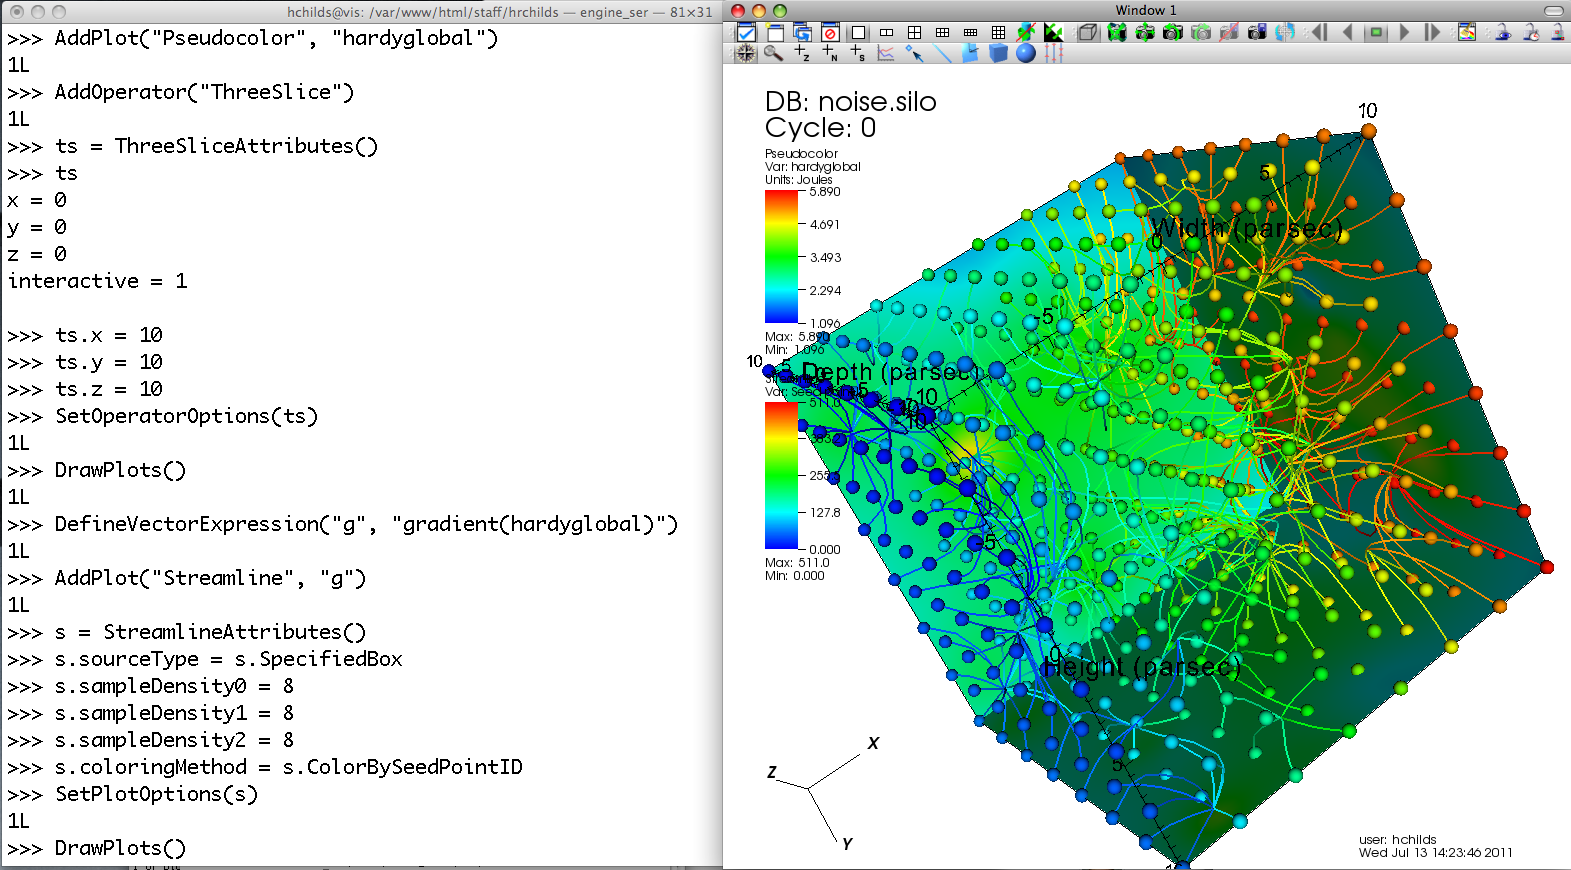
\includegraphics[width=4.8in]{teaser.png}
\end{DUlineblock}


\bigskip\hrule{}\bigskip


\begin{DUlineblock}{0em}
\item[] Version 2.10.0
\end{DUlineblock}


\bigskip\hrule{}\bigskip



\chapter{Introduction to VisIt}
\label{intro:pythonmanual}\label{intro::doc}\label{intro:visit-python-interface-manual}\label{intro:introduction-to-visit}

\section{Overview}
\label{intro:overview}
VisIt is a distributed, parallel, visualization tool for visualizing
data defined on two and three-dimensional structured and unstructured
meshes. VisIt’s distributed architecture allows it to leverage both the
compute power of a large parallel computer and the graphics acceleration
hardware of a local workstation. Another benefit of the distributed
architecture is that VisIt can visualize the data where it is generated,
eliminating the need to move data. VisIt can be controlled by a
Graphical User Interface (GUI) or through the Python scripting language.
More information about VisIt’s Graphical User Interface can be found in
the \emph{VisIt User’s Manual}.


\section{Manual chapters}
\label{intro:manual-chapters}
This manual is broken down into the following chapters:

\begin{tabulary}{\linewidth}{|L|L|}
\hline
\textsf{\relax 
Chapter title
} & \textsf{\relax 
Chapter description
}\\
\hline
Introduction to VisIt
 & 
This chapter.
\\
\hline
Python
 & 
Describes the basic features of the
\\
\hline & 
Python programming language.
\\
\hline
Quick Recipes
 & 
Describes common patterns for scripting
\\
\hline & 
using the VisIt Python Interface.
\\
\hline
Functions
 & 
Describes functions in the VisIt Python
\\
\hline & 
Interface.
\\
\hline
Attributes References
 & 
Describes attributes for setting common
\\
\hline & 
operations, as well as for VisIt’s plugins
\\
\hline
CLI Events
 & 
Describes possible events for callbacks.
\\
\hline\end{tabulary}



\section{Understanding how VisIt works}
\label{intro:understanding-how-visit-works}
VisIt visualizes data by creating one or more plots in a visualization
window, also known as a vis window. Examples of plots include Mesh
plots, Contour plots and Pseudocolor plots. Plots take as input one or
more mesh, material, scalar, or tensor variables. It is possible to
modify the variables by applying one or more operators to the variables
before passing them to a plot. Examples of operators include arithmetic
operations or taking slices through the mesh. It is also possible to
restrict the visualization of the data to subsets of the mesh. VisIt
provides Python bindings to all of its plots and operators so they may
be controlled through scripting. Each plot or operator plugin provides a
function, which is added to the VisIt namespace, to create the right
type of plot or operator attributes. The attribute object can then be
modified by setting its fields and then it can be passed to a
general-purpose function to set the plot or operator attributes. To
display a complete list of functions in the VisIt Python Interface, you
can type dir() at the Python prompt. Similarly, to inspect the contents
of any object, you can type its name at the Python prompt. VisIt
supports up to 16 visualization windows, also called vis windows. Each
vis window is independent of the other vis windows and VisIt Python
functions generally apply only to the currently active vis window. This
manual explains how to use the VisIt Python Interface which is a Python
extension module that controls VisIt’s viewer. In that way, the VisIt
Python Interface fulfills the same role as VisIt’s GUI. The difference
is that the viewer is totally controlled through Python scripting, which
makes it easy to write scripts to create visualizations and even movies.
Since the VisIt module controls VisIt’s viewer, the Python interpreter
currently has no direct mechanism for passing data to the compute engine
(see Figure {\hyperref[intro:fig:architecture]{\emph{{[}fig:architecture{]}}}}). If you want to
write a script that generates simulation data and have that script pass
data to the compute engine, you must pass the data through a file on
disk. The VisIt Python Interface comes packaged in two varieties: the
extension module and the Command Line Interface (CLI). The extension
module version of the VisIt Python Interface is imported into a standard
Python interpreter using the import directive. VisIt’s command line
interface (CLI) is essentially a Python interpreter where the VisIt
Python Interface is built-in. The CLI is provided to simplify the
process of running VisIt Python scripts.
\centering\begin{figure}[htbp]
\centering
\capstart

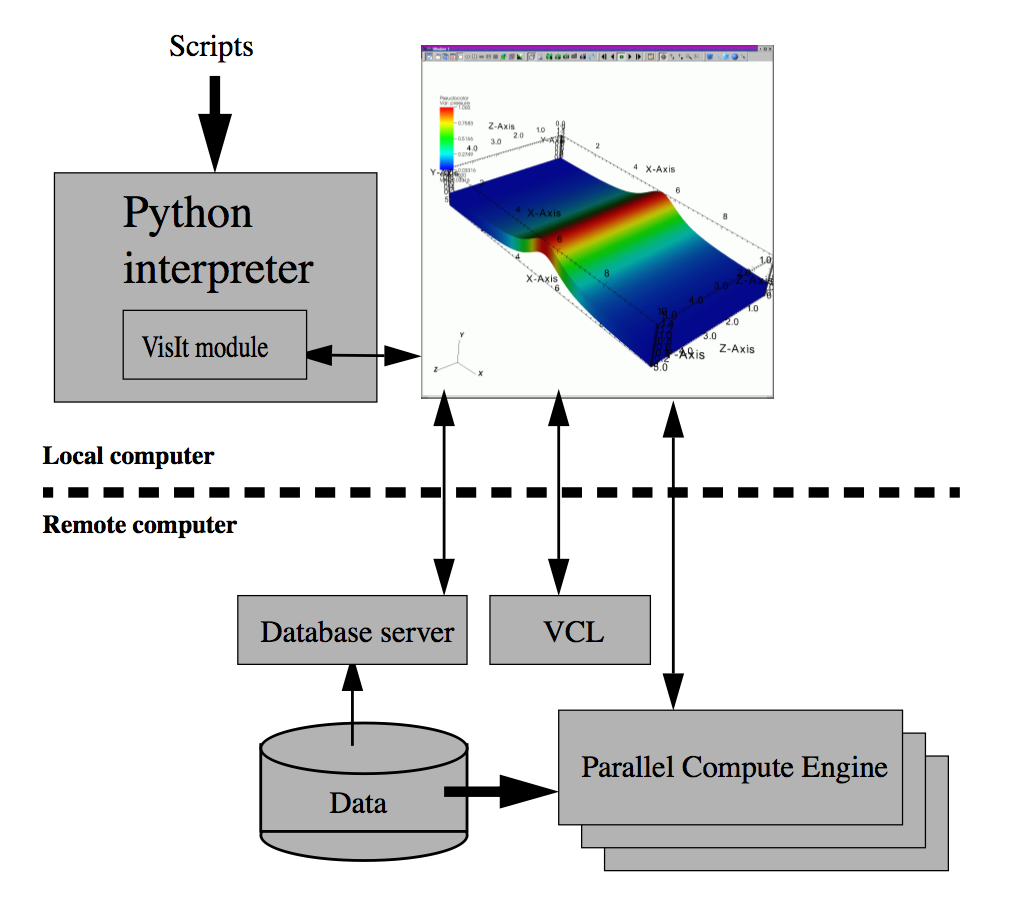
\includegraphics{architecture.png}
\caption{VisIt’s architecture}\end{figure}


\section{Starting VisIt}
\label{intro:starting-visit}
You can invoke VisIt’s command line interface from the command line by
typing:

\begin{Verbatim}[commandchars=\\\{\}]
\PYG{n}{visit} \PYG{o}{\PYGZhy{}}\PYG{n}{cli}
\end{Verbatim}

VisIt provides a separate Python module if you instead wish to include
VisIt functions in an existing Python script. In that case, you must
first import the VisIt module into Python and then call the Launch()
function to make VisIt launch and dynamically load the rest of the VisIt
functions into the Python namespace. VisIt adopts this somewhat unusual
approach to module loading since the lightweight “visit'' front-end
module can be installed as one of your Python’s site packages yet still
dynamically load the real control functions from different versions of
VisIt selected by the user.

If you do not install the visit.so module as a Python site package, you
can tell the Python interpreter where it is located by appending a new
path to the sys.path variable. Be sure to substitute the correct path to
visit.so on your system.

\begin{Verbatim}[commandchars=\\\{\}]
\PYG{k+kn}{import} \PYG{n+nn}{sys}
\PYG{n}{sys}\PYG{o}{.}\PYG{n}{path}\PYG{o}{.}\PYG{n}{append}\PYG{p}{(}\PYG{l+s+s2}{\PYGZdq{}}\PYG{l+s+s2}{/path/to/visit/\PYGZlt{}version\PYGZgt{}/\PYGZlt{}architecture\PYGZgt{}/lib/site\PYGZhy{}packages}\PYG{l+s+s2}{\PYGZdq{}}\PYG{p}{)}
\end{Verbatim}

Here is how to import all functions into the global Python namespace:

\begin{Verbatim}[commandchars=\\\{\}]
\PYG{k+kn}{from} \PYG{n+nn}{visit} \PYG{k+kn}{import} \PYG{o}{*}
\PYG{n}{Launch}\PYG{p}{(}\PYG{p}{)}
\end{Verbatim}

Here is how to import all functions into a “visit'' module namespace:

\begin{Verbatim}[commandchars=\\\{\}]
\PYG{k+kn}{import} \PYG{n+nn}{visit}
\PYG{n}{visit}\PYG{o}{.}\PYG{n}{Launch}\PYG{p}{(}\PYG{p}{)}
\end{Verbatim}


\section{Getting started}
\label{intro:getting-started}
VisIt is a tool for visualizing 2D and 3D scientific databases. The
first thing to do when running VisIt is select databases to visualize.
To select a database, you must first open the database using the
OpenDatabase function. After a window has an open database, any number
of plots and operators can be added. To create a plot, use the AddPlot
function. After adding a plot, call the DrawPlots function to make sure
that all of the new plots are drawn.

Example:

\begin{Verbatim}[commandchars=\\\{\}]
\PYG{n}{OpenDatabase}\PYG{p}{(}\PYG{l+s+s2}{\PYGZdq{}}\PYG{l+s+s2}{/usr/local/visit/data/multi\PYGZus{}curv3d.silo}\PYG{l+s+s2}{\PYGZdq{}}\PYG{p}{)}
\PYG{n}{AddPlot}\PYG{p}{(}\PYG{l+s+s2}{\PYGZdq{}}\PYG{l+s+s2}{Pseudocolor}\PYG{l+s+s2}{\PYGZdq{}}\PYG{p}{,} \PYG{l+s+s2}{\PYGZdq{}}\PYG{l+s+s2}{u}\PYG{l+s+s2}{\PYGZdq{}}\PYG{p}{)}
\PYG{n}{DrawPlots}\PYG{p}{(}\PYG{p}{)}
\end{Verbatim}

To see a list of the available plots and operators when you use the
VisIt Python Interface, use the Operator Plugins and Plot Plugins
functions. Each of those functions returns a tuple of strings that
contain the names of the currently loaded plot or operator plugins. Each
plot and operator plugin provides a function for creating an attributes
object to set the plot or operator attributes. The name of the function
is the name of the plugin in the tuple returned by the OperatorPlugins
or PlotPlugins functions plus the word “Attributes''. For example, the
“Pseudocolor'' plot provides a function called PseudocolorAttributes. To
set the plot attributes or the operator attributes, first use the
attributes creation function to create an attributes object. Assign the
newly created object to a variable name and set the fields in the
object. Each object has its own set of fields. To see the available
fields in an object, print the name of the variable at the Python prompt
and press the Enter key. This will print the contents of the object so
you can see the fields contained by the object. After setting the
appropriate fields, pass the object to either the SetPlotOptions
function or the SetOperatorAttributes function.

Example:

\begin{Verbatim}[commandchars=\\\{\}]
\PYG{n}{OpenDatabase}\PYG{p}{(}\PYG{l+s+s2}{\PYGZdq{}}\PYG{l+s+s2}{/usr/local/visit/data/globe.silo}\PYG{l+s+s2}{\PYGZdq{}}\PYG{p}{)}
\PYG{n}{AddPlot}\PYG{p}{(}\PYG{l+s+s2}{\PYGZdq{}}\PYG{l+s+s2}{Pseudocolor}\PYG{l+s+s2}{\PYGZdq{}}\PYG{p}{,} \PYG{l+s+s2}{\PYGZdq{}}\PYG{l+s+s2}{u}\PYG{l+s+s2}{\PYGZdq{}}\PYG{p}{)}
\PYG{n}{AddOperator}\PYG{p}{(}\PYG{l+s+s2}{\PYGZdq{}}\PYG{l+s+s2}{Slice}\PYG{l+s+s2}{\PYGZdq{}}\PYG{p}{)}
\PYG{n}{p} \PYG{o}{=} \PYG{n}{PseudocolorAttributes}\PYG{p}{(}\PYG{p}{)}
\PYG{n}{p}\PYG{o}{.}\PYG{n}{colorTableName} \PYG{o}{=} \PYG{l+s+s2}{\PYGZdq{}}\PYG{l+s+s2}{rainbow}\PYG{l+s+s2}{\PYGZdq{}}
\PYG{n}{p}\PYG{o}{.}\PYG{n}{opacity} \PYG{o}{=} \PYG{l+m+mf}{0.5}
\PYG{n}{SetPlotOptions}\PYG{p}{(}\PYG{n}{p}\PYG{p}{)}
\PYG{n}{a} \PYG{o}{=} \PYG{n}{SliceAttributes}\PYG{p}{(}\PYG{p}{)}
\PYG{n}{a}\PYG{o}{.}\PYG{n}{originType} \PYG{o}{=} \PYG{n}{a}\PYG{o}{.}\PYG{n}{Point}
\PYG{n}{a}\PYG{o}{.}\PYG{n}{normal}\PYG{p}{,} \PYG{n}{a}\PYG{o}{.}\PYG{n}{upAxis} \PYG{o}{=} \PYG{p}{(}\PYG{l+m+mi}{1}\PYG{p}{,}\PYG{l+m+mi}{1}\PYG{p}{,}\PYG{l+m+mi}{1}\PYG{p}{)}\PYG{p}{,} \PYG{p}{(}\PYG{o}{\PYGZhy{}}\PYG{l+m+mi}{1}\PYG{p}{,}\PYG{l+m+mi}{1}\PYG{p}{,}\PYG{o}{\PYGZhy{}}\PYG{l+m+mi}{1}\PYG{p}{)}
\PYG{n}{SetOperatorOptions}\PYG{p}{(}\PYG{n}{a}\PYG{p}{)}
\PYG{n}{DrawPlots}\PYG{p}{(}\PYG{p}{)}
\end{Verbatim}

That’s all there is to creating a plot using VisIt’s Python Interface.
For more information on creating plots and performing specific actions
in VisIt, refer to the documentation for each function later in this
manual.


\chapter{Python}
\label{python:python}\label{python::doc}\label{python:visit}

\section{Overview}
\label{python:overview}
Python is a general purpose, interpreted, extensible, object-oriented
scripting language that was chosen for VisIt’s scripting language due to
its ease of use and flexibility. VisIt’s Python interface was
implemented as Python module and it allows you to enhance your Python
scripts with coding to control VisIt. This chapter explains some of
Python’s syntax so it will be more familiar when you examine the
examples found in this document. For more information on programming in
Python, there are a number of good references, including on the Internet
at \href{http://www.python.org}{http://www.python.org}.


\section{Indentation}
\label{python:indentation}
One of the most obvious features of Python is its use of indentation for
new scopes. You must take special care to indent all program logic
consistently or else the Python interpreter may halt with an error, or
worse, not do what you intended. You must increase indentation levels
when you define a function, use an if/elif/else statement, or use any
loop construct.

Note the different levels of indentation:

\begin{Verbatim}[commandchars=\\\{\}]
\PYG{k}{def} \PYG{n+nf}{example\PYGZus{}function}\PYG{p}{(}\PYG{n}{n}\PYG{p}{)}\PYG{p}{:}
  \PYG{n}{v} \PYG{o}{=} \PYG{l+m+mi}{0}
  \PYG{k}{if} \PYG{n}{n} \PYG{o}{\PYGZgt{}} \PYG{l+m+mi}{2}\PYG{p}{:}
    \PYG{k}{print} \PYG{l+s+s2}{\PYGZdq{}}\PYG{l+s+s2}{n greater than 2.}\PYG{l+s+s2}{\PYGZdq{}}
  \PYG{k}{else}\PYG{p}{:}
    \PYG{n}{v} \PYG{o}{=} \PYG{n}{n} \PYG{o}{*} \PYG{n}{n}
  \PYG{k}{return} \PYG{n}{v}
\end{Verbatim}


\section{Comments}
\label{python:comments}
Like all good programming languages, Python supports the addition of
comments in the code. Comments begin with a pound character (\#) and
continue to the end of the line.

\begin{Verbatim}[commandchars=\\\{\}]
\PYG{c+c1}{\PYGZsh{} This is a comment}
\PYG{n}{a} \PYG{o}{=} \PYG{l+m+mi}{5} \PYG{o}{*} \PYG{l+m+mi}{5}
\end{Verbatim}


\section{Identifiers}
\label{python:identifiers}
The Python interpreter accepts any identifier that contains letters
’A’-’Z’, ’a’-’z’ and numbers ’0’-’9’ as long as the identifier does not
begin with a number. The Python interpreter is case-sensitive so the
identifier “case'' would not be the same identifier as “CASE''. Be sure to
case consistently throughout your Python code since the Python
interpreter will instantiate any identifier that it has not seen before
and mixing case would cause the interpreter to use multiple identifiers
and cause problems that you might not expect. Identifiers can be used to
refer to any type of object since Python is flexible in its treatment of
types.


\section{Data types}
\label{python:data-types}
Python supports a wide variety of data types and allows you to define
your own data types readily. Most types are created from a handful of
building-block types such as integers, floats, strings, tuples, lists,
and dictionaries.


\subsection{Strings}
\label{python:strings}
Python has built-in support for strings and you can create them using
single quotes or double quotes. You can even use both types of quotes so
you can create strings that include quotes in case quotes are desired in
the output. Strings are sequence objects and support operations that can
break them down into characters.

\begin{Verbatim}[commandchars=\\\{\}]
\PYG{n}{s} \PYG{o}{=} \PYG{l+s+s1}{\PYGZsq{}}\PYG{l+s+s1}{using single quotes}\PYG{l+s+s1}{\PYGZsq{}}
\PYG{n}{s2} \PYG{o}{=} \PYG{l+s+s2}{\PYGZdq{}}\PYG{l+s+s2}{using double quotes}\PYG{l+s+s2}{\PYGZdq{}}
\PYG{n}{s3} \PYG{o}{=} \PYG{l+s+s1}{\PYGZsq{}}\PYG{l+s+s1}{nesting the }\PYG{l+s+s1}{\PYGZdq{}}\PYG{l+s+s1}{spiffy}\PYG{l+s+s1}{\PYGZdq{}}\PYG{l+s+s1}{ double quotes}\PYG{l+s+s1}{\PYGZsq{}}
\end{Verbatim}


\subsection{Tuples}
\label{python:tuples}
Python supports tuples, which can be thought of as a read-only set of
objects. The members of a tuple can be of different types. Tuples are
commonly used to group multiple related items into a single object that
can be passed around more easily. Tuples support a number of operations.
You can subscript a tuple like an array to access its individual
members. You can easily determine whether an object is a member of a
tuple. You can iterate over a tuple. There are many more uses for
tuples. You can create tuples by enclosing a comma-separated list of
objects in parenthesis.

\begin{Verbatim}[commandchars=\\\{\}]
\PYG{c+c1}{\PYGZsh{} Create a tuple}
\PYG{n}{a} \PYG{o}{=} \PYG{p}{(}\PYG{l+m+mi}{1}\PYG{p}{,}\PYG{l+m+mi}{2}\PYG{p}{,}\PYG{l+m+mi}{3}\PYG{p}{,}\PYG{l+m+mi}{4}\PYG{p}{,}\PYG{l+m+mi}{5}\PYG{p}{)}
\PYG{k}{print} \PYG{l+s+s2}{\PYGZdq{}}\PYG{l+s+s2}{The first value in a is:}\PYG{l+s+s2}{\PYGZdq{}}\PYG{p}{,} \PYG{n}{a}\PYG{p}{[}\PYG{l+m+mi}{0}\PYG{p}{]}
\PYG{c+c1}{\PYGZsh{} See if 3 is in a using the \PYGZdq{}in\PYGZdq{} operator.}
\PYG{k}{print} \PYG{l+s+s2}{\PYGZdq{}}\PYG{l+s+s2}{3 is in a:}\PYG{l+s+s2}{\PYGZdq{}}\PYG{p}{,} \PYG{l+m+mi}{3} \PYG{o+ow}{in} \PYG{n}{a}
\PYG{c+c1}{\PYGZsh{} Create another tuple and add it to the first one to create c.}
\PYG{n}{b} \PYG{o}{=} \PYG{p}{(}\PYG{l+m+mi}{6}\PYG{p}{,}\PYG{l+m+mi}{7}\PYG{p}{,}\PYG{l+m+mi}{8}\PYG{p}{,}\PYG{l+m+mi}{9}\PYG{p}{)}
\PYG{n}{c} \PYG{o}{=} \PYG{n}{a} \PYG{o}{+} \PYG{n}{b}
\PYG{c+c1}{\PYGZsh{} Iterate over the items in the tuple}
\PYG{k}{for} \PYG{n}{value} \PYG{o+ow}{in} \PYG{n}{c}\PYG{p}{:}
  \PYG{k}{print} \PYG{l+s+s2}{\PYGZdq{}}\PYG{l+s+s2}{value is: }\PYG{l+s+s2}{\PYGZdq{}}\PYG{p}{,} \PYG{n}{value}
\end{Verbatim}


\subsection{Lists}
\label{python:lists}
Lists are just like tuples except they are not read-only and they use
square brackets {[}{]} to enclose the items in the list instead of using
parenthesis.

\begin{Verbatim}[commandchars=\\\{\}]
\PYG{c+c1}{\PYGZsh{} Start with an empty list.}
\PYG{n}{L} \PYG{o}{=} \PYG{p}{[}\PYG{p}{]}
\PYG{k}{for} \PYG{n}{i} \PYG{o+ow}{in} \PYG{n+nb}{range}\PYG{p}{(}\PYG{l+m+mi}{10}\PYG{p}{)}\PYG{p}{:}
  \PYG{c+c1}{\PYGZsh{} Add i to the list L}
  \PYG{n}{L} \PYG{o}{=} \PYG{n}{L} \PYG{o}{+} \PYG{p}{[}\PYG{n}{i}\PYG{p}{]}
\PYG{k}{print} \PYG{n}{L}
\PYG{c+c1}{\PYGZsh{} Assign a value into element 6}
\PYG{n}{L}\PYG{p}{[}\PYG{l+m+mi}{5}\PYG{p}{]} \PYG{o}{=} \PYG{l+m+mi}{1000}
\PYG{k}{print} \PYG{n}{L}
\end{Verbatim}


\subsection{Dictionaries}
\label{python:dictionaries}
Dictionaries are Python containers that allow you to store a value that
is associated with a key. Dictionaries are convenient for mapping 1 set
to another set since they allow you to perform easy lookups of values.
Dictionaries are declared using curly braces and each item in the
dictionary consists of a key: value pair with the key and values being
separated by a colon. To perform a lookup using a dictionary, provide
the key whose value you want to look up to the subscript {[}{]} operator.

\begin{Verbatim}[commandchars=\\\{\}]
\PYG{n}{colors} \PYG{o}{=} \PYG{p}{\PYGZob{}}\PYG{l+s+s2}{\PYGZdq{}}\PYG{l+s+s2}{red}\PYG{l+s+s2}{\PYGZdq{}} \PYG{p}{:} \PYG{l+s+s2}{\PYGZdq{}}\PYG{l+s+s2}{rouge}\PYG{l+s+s2}{\PYGZdq{}}\PYG{p}{,} \PYG{l+s+s2}{\PYGZdq{}}\PYG{l+s+s2}{orange}\PYG{l+s+s2}{\PYGZdq{}} \PYG{p}{:} \PYG{l+s+s2}{\PYGZdq{}}\PYG{l+s+s2}{orange}\PYG{l+s+s2}{\PYGZdq{}}\PYG{p}{,} \PYGZbs{}
\PYG{l+s+s2}{\PYGZdq{}}\PYG{l+s+s2}{yellow}\PYG{l+s+s2}{\PYGZdq{}} \PYG{p}{:} \PYG{l+s+s2}{\PYGZdq{}}\PYG{l+s+s2}{jaune}\PYG{l+s+s2}{\PYGZdq{}}\PYG{p}{,} \PYG{l+s+s2}{\PYGZdq{}}\PYG{l+s+s2}{green}\PYG{l+s+s2}{\PYGZdq{}} \PYG{p}{:} \PYG{l+s+s2}{\PYGZdq{}}\PYG{l+s+s2}{vert}\PYG{l+s+s2}{\PYGZdq{}}\PYG{p}{,} \PYG{l+s+s2}{\PYGZdq{}}\PYG{l+s+s2}{blue}\PYG{l+s+s2}{\PYGZdq{}} \PYG{p}{:} \PYG{l+s+s2}{\PYGZdq{}}\PYG{l+s+s2}{bleu}\PYG{l+s+s2}{\PYGZdq{}}\PYG{p}{\PYGZcb{}}
\PYG{c+c1}{\PYGZsh{} Perform lookups using the keys.}
\PYG{k}{for} \PYG{n}{c} \PYG{o+ow}{in} \PYG{n}{colors}\PYG{o}{.}\PYG{n}{keys}\PYG{p}{(}\PYG{p}{)}\PYG{p}{:}
   \PYG{k}{print} \PYG{l+s+s2}{\PYGZdq{}}\PYG{l+s+si}{\PYGZpc{}s}\PYG{l+s+s2}{ in French is: }\PYG{l+s+si}{\PYGZpc{}s}\PYG{l+s+s2}{\PYGZdq{}} \PYG{o}{\PYGZpc{}} \PYG{p}{(}\PYG{n}{c}\PYG{p}{,} \PYG{n}{colors}\PYG{p}{[}\PYG{n}{c}\PYG{p}{]}\PYG{p}{)}
\end{Verbatim}


\section{Control flow}
\label{python:control-flow}
Python, like other general-purpose programming languages provides
keywords that implement control flow. Control flow is an important
feature to have in a programming language because it allows complex
behavior to be created using a minimum amount of scripting.


\subsection{if/elif/else}
\label{python:if-elif-else}
Python provides if/elif/else for conditional branching. The if statement
takes any expression that evaluates to an integer and it takes the if
branch if the integer value is 1 other wise it takes the else branch if
it is present.

\begin{Verbatim}[commandchars=\\\{\}]
\PYG{c+c1}{\PYGZsh{} Example 1}
\PYG{k}{if} \PYG{n}{condition}\PYG{p}{:}
     \PYG{n}{do\PYGZus{}something}\PYG{p}{(}\PYG{p}{)}

\PYG{c+c1}{\PYGZsh{} Example 2}
\PYG{k}{if} \PYG{n}{condition}\PYG{p}{:}
     \PYG{n}{do\PYGZus{}something}\PYG{p}{(}\PYG{p}{)}
\PYG{k}{else}\PYG{p}{:}
     \PYG{n}{do\PYGZus{}something\PYGZus{}else}\PYG{p}{(}\PYG{p}{)}

\PYG{c+c1}{\PYGZsh{} Example 3}
\PYG{k}{if} \PYG{n}{condition}\PYG{p}{:}
     \PYG{n}{do\PYGZus{}domething}\PYG{p}{(}\PYG{p}{)}
\PYG{k}{elif} \PYG{n}{conditionn}\PYG{p}{:}
     \PYG{n}{do\PYGZus{}something\PYGZus{}n}\PYG{p}{(}\PYG{p}{)}
\PYG{k}{else}\PYG{p}{:}
     \PYG{n}{do\PYGZus{}something\PYGZus{}else}\PYG{p}{(}\PYG{p}{)}
\end{Verbatim}


\subsection{For loop}
\label{python:for-loop}
Python provides a for loop that allows you to iterate over all items
stored in a sequence object (tuples, lists, strings). The body of the
for loop executes once for each item in the sequence object and allows
you to specify the name of an identifier to use in order to reference
the current item.

\begin{Verbatim}[commandchars=\\\{\}]
\PYG{c+c1}{\PYGZsh{} Iterating through the characters of a string}
\PYG{k}{for} \PYG{n}{c} \PYG{o+ow}{in} \PYG{l+s+s2}{\PYGZdq{}}\PYG{l+s+s2}{characters}\PYG{l+s+s2}{\PYGZdq{}}\PYG{p}{:}
   \PYG{k}{print} \PYG{n}{c}

\PYG{c+c1}{\PYGZsh{} Iterating through a tuple}
\PYG{k}{for} \PYG{n}{value} \PYG{o+ow}{in} \PYG{p}{(}\PYG{l+s+s2}{\PYGZdq{}}\PYG{l+s+s2}{VisIt}\PYG{l+s+s2}{\PYGZdq{}}\PYG{p}{,} \PYG{l+s+s2}{\PYGZdq{}}\PYG{l+s+s2}{is}\PYG{l+s+s2}{\PYGZdq{}}\PYG{p}{,} \PYG{l+s+s2}{\PYGZdq{}}\PYG{l+s+s2}{coolness}\PYG{l+s+s2}{\PYGZdq{}}\PYG{p}{,} \PYG{l+s+s2}{\PYGZdq{}}\PYG{l+s+s2}{times}\PYG{l+s+s2}{\PYGZdq{}}\PYG{p}{,} \PYG{l+m+mi}{100}\PYG{p}{)}\PYG{p}{:}
   \PYG{k}{print} \PYG{n}{value}

\PYG{c+c1}{\PYGZsh{} Iterating through a list}
\PYG{k}{for} \PYG{n}{value} \PYG{o+ow}{in} \PYG{p}{[}\PYG{l+s+s2}{\PYGZdq{}}\PYG{l+s+s2}{VisIt}\PYG{l+s+s2}{\PYGZdq{}}\PYG{p}{,} \PYG{l+s+s2}{\PYGZdq{}}\PYG{l+s+s2}{is}\PYG{l+s+s2}{\PYGZdq{}}\PYG{p}{,} \PYG{l+s+s2}{\PYGZdq{}}\PYG{l+s+s2}{coolness}\PYG{l+s+s2}{\PYGZdq{}}\PYG{p}{,} \PYG{l+s+s2}{\PYGZdq{}}\PYG{l+s+s2}{times}\PYG{l+s+s2}{\PYGZdq{}}\PYG{p}{,} \PYG{l+m+mi}{100}\PYG{p}{]}\PYG{p}{:}
   \PYG{k}{print} \PYG{n}{value}

\PYG{c+c1}{\PYGZsh{} Iterating through a range of numbers [0,N) created with range(N).}
\PYG{n}{N} \PYG{o}{=} \PYG{l+m+mi}{100}
\PYG{k}{for} \PYG{n}{i} \PYG{o+ow}{in} \PYG{n+nb}{range}\PYG{p}{(}\PYG{n}{N}\PYG{p}{)}\PYG{p}{:}
   \PYG{k}{print} \PYG{n}{i}\PYG{p}{,} \PYG{n}{i}\PYG{o}{*}\PYG{n}{i}
\end{Verbatim}


\subsection{While loop}
\label{python:while-loop}
Python provides a while loop that allows you to execute a loop body
indefinitely based on some condition. The while loop can be used for
iteration but can also be used to execute more complex types of loops.

\begin{Verbatim}[commandchars=\\\{\}]
\PYG{n}{token} \PYG{o}{=} \PYG{n}{get\PYGZus{}next\PYGZus{}token}\PYG{p}{(}\PYG{p}{)}
\PYG{k}{while} \PYG{n}{token} \PYG{o}{!=} \PYG{l+s+s2}{\PYGZdq{}}\PYG{l+s+s2}{\PYGZdq{}}\PYG{p}{:}
  \PYG{n}{do\PYGZus{}something}\PYG{p}{(}\PYG{n}{token}\PYG{p}{)}
  \PYG{n}{token} \PYG{o}{=} \PYG{n}{get\PYGZus{}next\PYGZus{}token}\PYG{p}{(}\PYG{p}{)}
\end{Verbatim}


\section{Functions}
\label{python:functions}
Python comes with many built-in functions and modules that implement
additional functions. Functions can be used to execute bodies of code
that are meant to be re-used. Functions can optionally take arguments
and can optionally return values. Python provides the def keyword, which
allows you to define a function. The def keyword is followed by the name
of the function and its arguments, which should appear as a tuple next
to the name of the function.

\begin{Verbatim}[commandchars=\\\{\}]
\PYG{c+c1}{\PYGZsh{} Define a function with no arguments and no return value.}
\PYG{k}{def} \PYG{n+nf}{my\PYGZus{}function}\PYG{p}{(}\PYG{p}{)}\PYG{p}{:}
    \PYG{k}{print} \PYG{l+s+s2}{\PYGZdq{}}\PYG{l+s+s2}{my function prints this...}\PYG{l+s+s2}{\PYGZdq{}}

\PYG{c+c1}{\PYGZsh{} Define a function with arguments and a return value.}
\PYG{k}{def} \PYG{n+nf}{n\PYGZus{}to\PYGZus{}the\PYGZus{}d\PYGZus{}power}\PYG{p}{(}\PYG{n}{n}\PYG{p}{,} \PYG{n}{d}\PYG{p}{)}\PYG{p}{:}
    \PYG{n}{value} \PYG{o}{=} \PYG{l+m+mi}{1}
    \PYG{k}{if} \PYG{n}{d} \PYG{o}{\PYGZgt{}} \PYG{l+m+mi}{0}\PYG{p}{:}
        \PYG{k}{for} \PYG{n}{i} \PYG{o+ow}{in} \PYG{n+nb}{range}\PYG{p}{(}\PYG{n}{d}\PYG{p}{)}\PYG{p}{:}
            \PYG{n}{value} \PYG{o}{=} \PYG{n}{value} \PYG{o}{*} \PYG{n}{n}
    \PYG{k}{elif} \PYG{n}{d} \PYG{o}{\PYGZlt{}} \PYG{l+m+mi}{0}\PYG{p}{:}
        \PYG{n}{value} \PYG{o}{=} \PYG{l+m+mf}{1.} \PYG{o}{/} \PYG{n+nb}{float}\PYG{p}{(}\PYG{n}{n\PYGZus{}to\PYGZus{}the\PYGZus{}d\PYGZus{}power}\PYG{p}{(}\PYG{n}{n}\PYG{p}{,} \PYG{o}{\PYGZhy{}}\PYG{n}{d}\PYG{p}{)}\PYG{p}{)}

\PYG{k}{return} \PYG{n}{value}
\end{Verbatim}


\chapter{Quick Recipes}
\label{quickrecipes::doc}\label{quickrecipes:quick-recipes}\label{quickrecipes:visit}

\section{Overview}
\label{quickrecipes:overview}
This manual contains documentation for over two hundred functions and
several dozen extension object types. Learning to combine the right
functions in order to accomplish a visualization task without guidance
would involve hours of trial and error. To maximize productivity and
start creating visualizations using Visit’s Python Interface as fast as
possible, this chapter provides some common patterns, or ``quick recipes''
that you can combine to quickly create complex scripts.


\section{How to start}
\label{quickrecipes:how-to-start}
The most important question when developing a script is: ``Where do I
start?''. You can either use session files that you used to save the
state of your visualization to initialize the plots before you start
scripting or you can script every aspect of plot initialization.


\subsection{Using session files}
\label{quickrecipes:using-session-files}
VisIt’s session files contain all of the information required to
recreate plots that have been set up in previous interactive VisIt
sessions. Since session files contain all of the information about
plots, etc., they are natural candidates to make scripting easier since
they can be used to do the hard part of setting up the complex
visualization, leaving the bulk of the script to animate through time or
alter the plots in some way. To use session files within a script, use
the RestoreSession function.

\begin{Verbatim}[commandchars=\\\{\}]
\PYG{c+c1}{\PYGZsh{} Import a session file from the current working directory.}
\PYG{n}{RestoreSesssion}\PYG{p}{(}\PYG{l+s+s2}{\PYGZdq{}}\PYG{l+s+s2}{my\PYGZus{}visualization.session}\PYG{l+s+s2}{\PYGZdq{}}\PYG{p}{,} \PYG{l+m+mi}{0}\PYG{p}{)}
\PYG{c+c1}{\PYGZsh{} Now that VisIt has restored the session, animate through time.}
\PYG{k}{for} \PYG{n}{states} \PYG{o+ow}{in} \PYG{n+nb}{range}\PYG{p}{(}\PYG{n}{TimeSliderGetNStates}\PYG{p}{(}\PYG{p}{)}\PYG{p}{)}\PYG{p}{:}
  \PYG{n}{SetTimeSliderState}\PYG{p}{(}\PYG{n}{state}\PYG{p}{)}
  \PYG{n}{SaveWindow}\PYG{p}{(}\PYG{p}{)}
\end{Verbatim}


\subsection{Getting something on the screen}
\label{quickrecipes:getting-something-on-the-screen}
If you don’t want to use a session file to begin the setup for your
visualization then you will have to dive into opening databases,
creating plots, and animating through time. This is where all of
hand-crafted scripts begin. The first step in creating a visualization
is opening a database. VisIt provides the OpenDatabase function to open
a database. Once a database has been opened, you can create plots from
its variables using the AddPlot function. The AddPlot function takes a
plot plugin name and the name of a variable from the open database. Once
you’ve added a plot, it is in the new state, which means that it has not
yet been submitted to the compute engine for processing. To make sure
that the plot gets drawn, call the DrawPlots function.

\begin{Verbatim}[commandchars=\\\{\}]
\PYG{c+c1}{\PYGZsh{} Step 1: Open a database}
\PYG{n}{OpenDatabase}\PYG{p}{(}\PYG{l+s+s2}{\PYGZdq{}}\PYG{l+s+s2}{/usr/local/visit/data/wave.visit}\PYG{l+s+s2}{\PYGZdq{}}\PYG{p}{)}

\PYG{c+c1}{\PYGZsh{} Step 2: Add plots}
\PYG{n}{AddPlot}\PYG{p}{(}\PYG{l+s+s2}{\PYGZdq{}}\PYG{l+s+s2}{Pseudocolor}\PYG{l+s+s2}{\PYGZdq{}}\PYG{p}{,} \PYG{l+s+s2}{\PYGZdq{}}\PYG{l+s+s2}{pressure}\PYG{l+s+s2}{\PYGZdq{}}\PYG{p}{)}
\PYG{n}{AddPlot}\PYG{p}{(}\PYG{l+s+s2}{\PYGZdq{}}\PYG{l+s+s2}{Mesh}\PYG{l+s+s2}{\PYGZdq{}}\PYG{p}{,} \PYG{l+s+s2}{\PYGZdq{}}\PYG{l+s+s2}{quadmesh}\PYG{l+s+s2}{\PYGZdq{}}\PYG{p}{)}

\PYG{c+c1}{\PYGZsh{} Step 3: Draw the plots}
\PYG{n}{DrawPlots}\PYG{p}{(}\PYG{p}{)}

\PYG{c+c1}{\PYGZsh{} Step 4: Animate through time and save images}
\PYG{k}{for} \PYG{n}{states} \PYG{o+ow}{in} \PYG{n+nb}{range}\PYG{p}{(}\PYG{n}{TimeSliderGetNStates}\PYG{p}{(}\PYG{p}{)}\PYG{p}{)}\PYG{p}{:}
  \PYG{n}{SetTimeSliderState}\PYG{p}{(}\PYG{n}{state}\PYG{p}{)}
  \PYG{n}{SaveWindow}\PYG{p}{(}\PYG{p}{)}
\end{Verbatim}


\section{Saving images}
\label{quickrecipes:saving-images}
Much of the time, the entire purpose of using VisIt’s Python Interface
is to create a script that can save out images of a time-varying
database for the purpose of making movies. Saving images using VisIt’s
Python Interface is a straight-forward process, involving just a few
functions.


\subsection{Setting the output image characteristics}
\label{quickrecipes:setting-the-output-image-characteristics}
VisIt provides a number of options for saving files, including:
fileformat, filename, and image size, to name a few. These attributes
are grouped into the SaveWindowAttributes object. To set the options
that VisIt uses to save files, you must create a SaveWindowAttributes
object, change the necessary attributes, and call the
SetSaveWindowAttributes function. Note that if you want to create images
using a specific image resolution, the best way is to use the
\emph{-geometry} command line argument with VisIt’s Command Line Interface
and tell VisIt to use screen capture. If you instead require your script
to be capable of saving everal different image sizes then you can turn
off screen capture and set the image resolution in the
SaveWindowAttributes object.

\begin{Verbatim}[commandchars=\\\{\}]
\PYG{c+c1}{\PYGZsh{} Save a BMP file at 1024x768 resolution}
\PYG{n}{s} \PYG{o}{=} \PYG{n}{SaveWindowAttributes}\PYG{p}{(}\PYG{p}{)}
\PYG{n}{s}\PYG{o}{.}\PYG{n}{format} \PYG{o}{=} \PYG{n}{s}\PYG{o}{.}\PYG{n}{BMP}
\PYG{n}{s}\PYG{o}{.}\PYG{n}{fileName} \PYG{o}{=} \PYG{l+s+s2}{\PYGZdq{}}\PYG{l+s+s2}{mybmpfile}\PYG{l+s+s2}{\PYGZdq{}}
\PYG{n}{s}\PYG{o}{.}\PYG{n}{width}\PYG{p}{,} \PYG{n}{s}\PYG{o}{.}\PYG{n}{height} \PYG{o}{=} \PYG{l+m+mi}{1024}\PYG{p}{,}\PYG{l+m+mi}{768}
\PYG{n}{s}\PYG{o}{.}\PYG{n}{screenCapture} \PYG{o}{=} \PYG{l+m+mi}{0}
\PYG{n}{SetSaveWindowAttributes}\PYG{p}{(}\PYG{n}{s}\PYG{p}{)}
\end{Verbatim}


\subsection{Saving an image}
\label{quickrecipes:saving-an-image}
Once you have set the SaveWindowAttributes to your liking, you can call
the SaveWindow function to save an image. The SaveWindow function
returns the name of the image that is saved so you can use that for
other purposes in your script.

\begin{Verbatim}[commandchars=\\\{\}]
\PYG{c+c1}{\PYGZsh{} Save images of all timesteps and add each image filename to a list.}
\PYG{n}{names} \PYG{o}{=} \PYG{p}{[}\PYG{p}{]}
\PYG{k}{for} \PYG{n}{state} \PYG{o+ow}{in} \PYG{n+nb}{range}\PYG{p}{(}\PYG{n}{TimeSliderGetNStates}\PYG{p}{(}\PYG{p}{)}\PYG{p}{)}\PYG{p}{:}
  \PYG{n}{SetTimeSliderState}\PYG{p}{(}\PYG{n}{state}\PYG{p}{)}
  \PYG{c+c1}{\PYGZsh{} Save the image}
  \PYG{n}{n} \PYG{o}{=} \PYG{n}{SaveWindow}\PYG{p}{(}\PYG{p}{)}
  \PYG{n}{names} \PYG{o}{=} \PYG{n}{names} \PYG{o}{+} \PYG{p}{[}\PYG{n}{n}\PYG{p}{]}
\PYG{k}{print} \PYG{n}{names}
\end{Verbatim}


\section{Working with databases}
\label{quickrecipes:working-with-databases}
VisIt allows you to open a wide array of databases both in terms of
supported file formats and in terms how databases treat time. Databases
can have a single time state or can have multiple time states. Databases
can natively support multiple time states or sets of single time states
files can be grouped into time-varying databases using .visit files or
using virtual databases. Working with databases gets even trickier if
you are using VisIt to visualize a database that is still being
generated by a simulation. This section describes how to interact with
databases.


\subsection{Opening a database}
\label{quickrecipes:opening-a-database}
Opening a database is a relatively simple operation - most complexities
arise in how the database treats time. If you only want to visualize a
single time state or if your database format natively supports multiple
timestates per file then opening a database requires just a single call
to the OpenDatabase function.

\begin{Verbatim}[commandchars=\\\{\}]
\PYG{c+c1}{\PYGZsh{} Open a database at time state 0}
\PYG{n}{OpenDatabase}\PYG{p}{(}\PYG{l+s+s2}{\PYGZdq{}}\PYG{l+s+s2}{/usr/local/visit/data/allinone00.pdb}\PYG{l+s+s2}{\PYGZdq{}}\PYG{p}{)}
\end{Verbatim}


\subsection{Opening a database at late time}
\label{quickrecipes:opening-a-database-at-late-time}
Opening a database at a later timestate is done just the same as opening
a database at time state zero except that you must specify the time
state at which you want to open the database. There are a number of
reasons for opening a database at a later time state. The most common
reason for doing so, as opposed to just changing time states later, is
that VisIt uses the metadata from the first opened time state to
describe the contents of the database for all timestates (except for
certain file formats that don’t do this, i.e. SAMRAI). This means that
the list of variables found for the first time state that you open is
used for all timestates. If your database contains a variable at a later
timestate that does not exist at earlier time states, you must open the
database at a later time state to gain access to the transient variable.

\begin{Verbatim}[commandchars=\\\{\}]
\PYG{c+c1}{\PYGZsh{} Open a database at a later time state to pick up transient variables}
\PYG{n}{OpenDatabase}\PYG{p}{(}\PYG{l+s+s2}{\PYGZdq{}}\PYG{l+s+s2}{/usr/local/visit/data/wave.visit}\PYG{l+s+s2}{\PYGZdq{}}\PYG{p}{,} \PYG{l+m+mi}{17}\PYG{p}{)}
\end{Verbatim}


\subsection{Opening a virtual database}
\label{quickrecipes:opening-a-virtual-database}
VisIt provides two ways for accessing a set of single time-state files
as a single time- varying database. The first method is a .visit file,
which is a simple text file that contains the names of each file to be
used as a time state in the time-varying database. The second method
uses ``virtual databases'', which allow VisIt to exploit the file naming
conventions that are often employed by simulation codes when they create
their dumps. In many cases, VisIt can scan a specified directory and
determine which filenames look related. Filenames with close matches are
grouped as individual time states into a virtual database whose name is
based on the more abstract pattern used to create the filenames.

\begin{Verbatim}[commandchars=\\\{\}]
\PYGZsh{} Opening first file in series wave0000.silo, wave0010.silo, ...
OpenDatabase(\PYGZdq{}/usr/local/visit/data/wave0000.silo\PYGZdq{})

\PYGZsh{} Opening a virtual database representing all wave*.silo files.
OpenDatabase(\PYGZdq{}/usr/local/visit/data/wave*.silo database.)
\end{Verbatim}


\subsection{Opening a remote database}
\label{quickrecipes:opening-a-remote-database}
VisIt supports running the client on a local computer while also
allowing you to process data in parallel on a remote computer. If you
want to access databases on a remote computer using VisIt’s Python
Interface, the only difference to accessing a database on a local
computer is that you must specify a host name as part of the database
name.

\begin{Verbatim}[commandchars=\\\{\}]
\PYG{c+c1}{\PYGZsh{} Opening a file on a remote computer by giving a host name}
\PYG{c+c1}{\PYGZsh{} Also, open the database to a later time slice (17)}
\PYG{n}{OpenDatabase}\PYG{p}{(}\PYG{l+s+s2}{\PYGZdq{}}\PYG{l+s+s2}{thunder:/usr/local/visit/data/wave.visit}\PYG{l+s+s2}{\PYGZdq{}}\PYG{p}{,} \PYG{l+m+mi}{17}\PYG{p}{)}
\end{Verbatim}


\subsection{Opening a compute engine}
\label{quickrecipes:opening-a-compute-engine}
Sometimes it is advantageous to open a compute engine before opening a
database. When you tell VisIt to open a database using the OpenDatabase
function, VisIt also launches a compute engine and tells the compute
engine to open the specified database. When the VisIt Python Interface
is run with a visible window, the \textbf{Engine Chooser Window} will present
itself so you can select a host profile. If you want to design a script
that must specify parallel options, etc in batch mode where there is no
\textbf{Engine ChooserWindow} then you have few options other than to open a
compute engine before opening a database. To open a compute engine, use
the OpenComputeEngine function. You can pass the name of the host on
which to run the compute engine and any arguments that must be used to
launch the engine such as the number of processors.

\begin{Verbatim}[commandchars=\\\{\}]
\PYG{c+c1}{\PYGZsh{} Open a remote, parallel compute engine before opening a database}
\PYG{n}{OpenComputeEngine}\PYG{p}{(}\PYG{l+s+s2}{\PYGZdq{}}\PYG{l+s+s2}{mcr}\PYG{l+s+s2}{\PYGZdq{}}\PYG{p}{,} \PYG{p}{(}\PYG{l+s+s2}{\PYGZdq{}}\PYG{l+s+s2}{\PYGZhy{}np}\PYG{l+s+s2}{\PYGZdq{}}\PYG{p}{,} \PYG{l+s+s2}{\PYGZdq{}}\PYG{l+s+s2}{4}\PYG{l+s+s2}{\PYGZdq{}}\PYG{p}{,} \PYG{l+s+s2}{\PYGZdq{}}\PYG{l+s+s2}{\PYGZhy{}nn}\PYG{l+s+s2}{\PYGZdq{}}\PYG{p}{,} \PYG{l+s+s2}{\PYGZdq{}}\PYG{l+s+s2}{2}\PYG{l+s+s2}{\PYGZdq{}}\PYG{p}{)}\PYG{p}{)}
\PYG{n}{OpenDatabase}\PYG{p}{(}\PYG{l+s+s2}{\PYGZdq{}}\PYG{l+s+s2}{mcr:/usr/local/visit/data/multi\PYGZus{}ucd3d.silo}\PYG{l+s+s2}{\PYGZdq{}}\PYG{p}{)}
\end{Verbatim}


\section{Working with plots}
\label{quickrecipes:working-with-plots}
Plots are viewable objects, created from a database, that can be
displayed in a visualization window. VisIt provides several types of
plots and each plot allows you to view data using different
visualization techniques. For example, the Pseudocolor plot allows you
to see the general shape of a simulated object while painting colors on
it according to the values stored in a variable’s scalar field. The most
important functions for interacting with plots are covered in this
section.


\subsection{Creating a plot}
\label{quickrecipes:creating-a-plot}
The function for adding a plot in VisIt is: AddPlot. The AddPlot
function takes the name of a plot type and the name of a variable that
is to be plotted and creates a new plot and adds it to the plot list.
The name of the plot to be created corresponds to the name of one of
VisIt’s plot plugins, which can be queried using the PlotPlugins
function. The variable that you pass to the AddPlot function must be a
valid variable for the opend atabase. New plots are not realized,
meaning that they have not been submitted to the compute engine for
processing. If you want to force VisIt to process the new plot you must
call the DrawPlots function.

\begin{Verbatim}[commandchars=\\\{\}]
\PYG{c+c1}{\PYGZsh{} Names of all available plot plugins}
\PYG{k}{print} \PYG{n}{PlotPlugins}\PYG{p}{(}\PYG{p}{)}
\PYG{c+c1}{\PYGZsh{} Create plots}
\PYG{n}{AddPlot}\PYG{p}{(}\PYG{l+s+s2}{\PYGZdq{}}\PYG{l+s+s2}{Pseudocolor}\PYG{l+s+s2}{\PYGZdq{}}\PYG{p}{,} \PYG{l+s+s2}{\PYGZdq{}}\PYG{l+s+s2}{pressure}\PYG{l+s+s2}{\PYGZdq{}}\PYG{p}{)}
\PYG{n}{AddPlot}\PYG{p}{(}\PYG{l+s+s2}{\PYGZdq{}}\PYG{l+s+s2}{Mesh}\PYG{l+s+s2}{\PYGZdq{}}\PYG{p}{,} \PYG{l+s+s2}{\PYGZdq{}}\PYG{l+s+s2}{quadmesh}\PYG{l+s+s2}{\PYGZdq{}}\PYG{p}{)}
\PYG{c+c1}{\PYGZsh{} Draw the plots}
\PYG{n}{DrawPlots}\PYG{p}{(}\PYG{p}{)}
\end{Verbatim}


\subsection{Plotting materials}
\label{quickrecipes:plotting-materials}
Plotting materials is a common operation in VisIt. The Boundary and
FilledBoundary plots enable you to plot material boundaries and
materials, respectively.

\begin{Verbatim}[commandchars=\\\{\}]
\PYG{c+c1}{\PYGZsh{} Plot material boundaries}
\PYG{n}{AddPlot}\PYG{p}{(}\PYG{l+s+s2}{\PYGZdq{}}\PYG{l+s+s2}{Boundary}\PYG{l+s+s2}{\PYGZdq{}}\PYG{p}{,} \PYG{l+s+s2}{\PYGZdq{}}\PYG{l+s+s2}{mat1}\PYG{l+s+s2}{\PYGZdq{}}\PYG{p}{)}
\PYG{c+c1}{\PYGZsh{} Plot materials}
\PYG{n}{AddPlot}\PYG{p}{(}\PYG{l+s+s2}{\PYGZdq{}}\PYG{l+s+s2}{FilledBoundary}\PYG{l+s+s2}{\PYGZdq{}}\PYG{p}{,} \PYG{l+s+s2}{\PYGZdq{}}\PYG{l+s+s2}{mat1}\PYG{l+s+s2}{\PYGZdq{}}\PYG{p}{)}
\end{Verbatim}


\subsection{Setting plot attributes}
\label{quickrecipes:setting-plot-attributes}
Each plot type has an attributes object that controls how the plot
generates its data or how it looks in the visualization window. The
attributes object for each plot contains different fields. You can view
the individual object fields by printing the object to the console. Each
plot type provides a function that creates a new instance of one of its
attribute objects. The function name is always of the form: plotname +
``Attributes''. For example, the attributes object creation function for
the Pseudocolor plot would be: PseudocolorAttributes. To change the
attributes for a plot, you create an attributes object using the
appropriate function, set the properties in the returned object, and
tell VisIt to use the new plot attributes by passing the object to the
SetPlotOptions function. Note that you should set a plot’s attributes
before calling the DrawPlots method to realize the plot since setting a
plot’s attributes can cause the compute engine to recalculate the plot.

\begin{Verbatim}[commandchars=\\\{\}]
\PYG{c+c1}{\PYGZsh{} Creating a Pseudocolor plot and setting min/max values.}
\PYG{n}{AddPlot}\PYG{p}{(}\PYG{l+s+s2}{\PYGZdq{}}\PYG{l+s+s2}{Pseudocolor}\PYG{l+s+s2}{\PYGZdq{}}\PYG{p}{,} \PYG{l+s+s2}{\PYGZdq{}}\PYG{l+s+s2}{pressure}\PYG{l+s+s2}{\PYGZdq{}}\PYG{p}{)}
\PYG{n}{p} \PYG{o}{=} \PYG{n}{PseudocolorAttributes}\PYG{p}{(}\PYG{p}{)}
\PYG{c+c1}{\PYGZsh{} Look in the object}
\PYG{k}{print} \PYG{n}{p}
\PYG{c+c1}{\PYGZsh{} Set the min/max values}
\PYG{n}{p}\PYG{o}{.}\PYG{n}{min}\PYG{p}{,} \PYG{n}{p}\PYG{o}{.}\PYG{n}{minFlag} \PYG{o}{=} \PYG{l+m+mf}{0.0}\PYG{p}{,} \PYG{l+m+mi}{1}
\PYG{n}{p}\PYG{o}{.}\PYG{n}{max}\PYG{p}{,} \PYG{n}{p}\PYG{o}{.}\PYG{n}{maxFlag} \PYG{o}{=} \PYG{l+m+mf}{10.0}\PYG{p}{,} \PYG{l+m+mi}{1}
\PYG{n}{SetPlotOptions}\PYG{p}{(}\PYG{n}{p}\PYG{p}{)}
\end{Verbatim}


\subsection{Working with multiple plots}
\label{quickrecipes:working-with-multiple-plots}
When you work with more than one plot, it is sometimes necessary to set
the active plots because some of VisIt’s functions apply to all of the
active plots. The active plot is usually the last plot that was created
unless you’ve changed the list of active plots. Changing which plots are
active is useful when you want to delete or hide certain plots or set
their plot attributes independently. When you want to set which plots
are active, use the SetActivePlots function. If you want to list the
plots that you’ve created, call the ListPlots function.

\begin{Verbatim}[commandchars=\\\{\}]
\PYG{c+c1}{\PYGZsh{} Create more than 1 plot of the same type}
\PYG{n}{AddPlot}\PYG{p}{(}\PYG{l+s+s2}{\PYGZdq{}}\PYG{l+s+s2}{Pseudocolor}\PYG{l+s+s2}{\PYGZdq{}}\PYG{p}{,} \PYG{l+s+s2}{\PYGZdq{}}\PYG{l+s+s2}{pressure}\PYG{l+s+s2}{\PYGZdq{}}\PYG{p}{)}
\PYG{n}{AddPlot}\PYG{p}{(}\PYG{l+s+s2}{\PYGZdq{}}\PYG{l+s+s2}{Pseudocolor}\PYG{l+s+s2}{\PYGZdq{}}\PYG{p}{,} \PYG{l+s+s2}{\PYGZdq{}}\PYG{l+s+s2}{density}\PYG{l+s+s2}{\PYGZdq{}}\PYG{p}{)}

\PYG{c+c1}{\PYGZsh{} List the plots. The second plot should be active.}
\PYG{n}{ListPlots}\PYG{p}{(}\PYG{p}{)}

\PYG{c+c1}{\PYGZsh{} Draw the plots}
\PYG{n}{DrawPlots}\PYG{p}{(}\PYG{p}{)}

\PYG{c+c1}{\PYGZsh{} Hide the first plot}
\PYG{n}{SetActivePlots}\PYG{p}{(}\PYG{l+m+mi}{0}\PYG{p}{)}
\PYG{n}{HideActivePlots}\PYG{p}{(}\PYG{p}{)}

\PYG{c+c1}{\PYGZsh{} Set both plots\PYGZsq{} color table to \PYGZdq{}hot\PYGZdq{}}
\PYG{n}{p} \PYG{o}{=} \PYG{n}{PseudocolorAttributes}\PYG{p}{(}\PYG{p}{)}
\PYG{n}{p}\PYG{o}{.}\PYG{n}{colorTableName} \PYG{o}{=} \PYG{l+s+s2}{\PYGZdq{}}\PYG{l+s+s2}{hot}\PYG{l+s+s2}{\PYGZdq{}}
\PYG{n}{SetActivePlots}\PYG{p}{(}\PYG{p}{(}\PYG{l+m+mi}{0}\PYG{p}{,}\PYG{l+m+mi}{1}\PYG{p}{)}\PYG{p}{)}
\PYG{n}{SetPlotOptions}\PYG{p}{(}\PYG{n}{p}\PYG{p}{)}

\PYG{c+c1}{\PYGZsh{} Show the first plot again.}
\PYG{n}{SetActivePlots}\PYG{p}{(}\PYG{l+m+mi}{0}\PYG{p}{)}
\PYG{n}{HideActivePlots}\PYG{p}{(}\PYG{p}{)}

\PYG{c+c1}{\PYGZsh{} Delete the second plot}
\PYG{n}{SetActivePlots}\PYG{p}{(}\PYG{l+m+mi}{1}\PYG{p}{)}
\PYG{n}{DeleteActivePlots}\PYG{p}{(}\PYG{p}{)}
\PYG{n}{ListPlots}\PYG{p}{(}\PYG{p}{)}
\end{Verbatim}


\subsection{Plots in the error state}
\label{quickrecipes:plots-in-the-error-state}
When VisIt’s compute engine cannot process a plot, the plot is put into
the error state. Once a plot is in the error state, it no longer is
displayed in the visualization window. If you are generating a movie,
plots entering the error state can be a serious problem because you most
often want all of the plots that you have created to animate through
time and not disappear in the middle of the animation. You can add extra
code to your script to prevent plots from disappearing (most of the
time) due to error conditions by adding a call to the DrawPlots
function.

\begin{Verbatim}[commandchars=\\\{\}]
\PYG{c+c1}{\PYGZsh{} Save an image and take care of plots that entered the error state.}
\PYG{n}{drawThePlots} \PYG{o}{=} \PYG{l+m+mi}{0}
\PYG{k}{for} \PYG{n}{state} \PYG{o+ow}{in} \PYG{n+nb}{range}\PYG{p}{(}\PYG{n}{TimeSliderGetNStates}\PYG{p}{(}\PYG{p}{)}\PYG{p}{)}\PYG{p}{:}
  \PYG{k}{if} \PYG{n}{SetTimeSliderState}\PYG{p}{(}\PYG{n}{state}\PYG{p}{)} \PYG{o}{==} \PYG{l+m+mi}{0}\PYG{p}{:}
    \PYG{n}{drawThePlots} \PYG{o}{=} \PYG{l+m+mi}{1}
  \PYG{k}{if} \PYG{n}{drawThePlots} \PYG{o}{==} \PYG{l+m+mi}{1}\PYG{p}{:}
    \PYG{k}{if} \PYG{n}{DrawPlots}\PYG{p}{(}\PYG{p}{)} \PYG{o}{==} \PYG{l+m+mi}{0}\PYG{p}{:}
      \PYG{k}{print} \PYG{l+s+s2}{\PYGZdq{}}\PYG{l+s+s2}{VisIt could not draw plots for state: }\PYG{l+s+si}{\PYGZpc{}d}\PYG{l+s+s2}{\PYGZdq{}} \PYG{o}{\PYGZpc{}} \PYG{n}{state}
    \PYG{k}{else}\PYG{p}{:}
      \PYG{n}{drawThePlots} \PYG{o}{=} \PYG{l+m+mi}{0}
  \PYG{n}{SaveWindow}\PYG{p}{(}\PYG{p}{)}
\end{Verbatim}


\section{Operators}
\label{quickrecipes:operators}
Operators are filters that are applied to database variables before the
compute engine uses them to create plots. Operators can be linked one
after the other to form chains of operators that can drastically
transform the data before plotting it.


\subsection{Adding operators}
\label{quickrecipes:adding-operators}
Adding an operator is similar to adding a plot in that you call a
function with the name of the operator to be added. The list of
available operators is returned by the OperatorPlugins function. Any of
the names returned in that plugin can be used to add an operator using
the AddOperator function. Operators are added to the active plots by
default but you can also force VisIt to add them to all plots in the
plot list.

\begin{Verbatim}[commandchars=\\\{\}]
\PYG{c+c1}{\PYGZsh{} Print available operators}
\PYG{k}{print} \PYG{n}{OperatorPlugins}\PYG{p}{(}\PYG{p}{)}
\PYG{c+c1}{\PYGZsh{} Create a plot}
\PYG{n}{AddPlot}\PYG{p}{(}\PYG{l+s+s2}{\PYGZdq{}}\PYG{l+s+s2}{Pseudocolor}\PYG{l+s+s2}{\PYGZdq{}}\PYG{p}{)}
\PYG{c+c1}{\PYGZsh{} Add an Isovolume operator and a Slice operator}
\PYG{n}{AddOperator}\PYG{p}{(}\PYG{l+s+s2}{\PYGZdq{}}\PYG{l+s+s2}{Isovolume}\PYG{l+s+s2}{\PYGZdq{}}\PYG{p}{)}
\PYG{n}{AddOperator}\PYG{p}{(}\PYG{l+s+s2}{\PYGZdq{}}\PYG{l+s+s2}{Slice}\PYG{l+s+s2}{\PYGZdq{}}\PYG{p}{)}
\PYG{n}{DrawPlots}\PYG{p}{(}\PYG{p}{)}
\end{Verbatim}


\subsection{Setting operator attributes}
\label{quickrecipes:setting-operator-attributes}
Each plot gets its own instance of an operator which means that you can
set each plot’s operator attributes independently. Like plots, operators
use objects to set their attributes. These objects are returned by
functions whose names are of the form: operatorname + ``Attributes''. Once
you have created an operator attributes object, you can pass it to the
SetOperatorOptions to set the options for an operator. Note that setting
the attributes for an operator nearly always causes the compute engine
to recalculate the operator. You can use the power of VisIt’s Python
Interface to create complex operator behavior such as in the following
code example, which moves slice planes through a Pseudocolor plot.

\begin{Verbatim}[commandchars=\\\{\}]
\PYG{n}{OpenDatabase}\PYG{p}{(}\PYG{l+s+s2}{\PYGZdq{}}\PYG{l+s+s2}{/usr/local/visit/data/noise.silo}\PYG{l+s+s2}{\PYGZdq{}}\PYG{p}{)}
\PYG{n}{AddPlot}\PYG{p}{(}\PYG{l+s+s2}{\PYGZdq{}}\PYG{l+s+s2}{Pseudocolor}\PYG{l+s+s2}{\PYGZdq{}}\PYG{p}{,} \PYG{l+s+s2}{\PYGZdq{}}\PYG{l+s+s2}{hardyglobal}\PYG{l+s+s2}{\PYGZdq{}}\PYG{p}{)}
\PYG{n}{AddOperator}\PYG{p}{(}\PYG{l+s+s2}{\PYGZdq{}}\PYG{l+s+s2}{Slice}\PYG{l+s+s2}{\PYGZdq{}}\PYG{p}{)}
\PYG{n}{s} \PYG{o}{=} \PYG{n}{SliceAttributes}\PYG{p}{(}\PYG{p}{)}
\PYG{n}{s}\PYG{o}{.}\PYG{n}{originType} \PYG{o}{=} \PYG{n}{s}\PYG{o}{.}\PYG{n}{Percent}
\PYG{n}{s}\PYG{o}{.}\PYG{n}{project2d} \PYG{o}{=} \PYG{l+m+mi}{0}
\PYG{n}{SetOperatorOptions}\PYG{p}{(}\PYG{n}{s}\PYG{p}{)}
\PYG{n}{DrawPlots}\PYG{p}{(}\PYG{p}{)}

\PYG{n}{nSteps} \PYG{o}{=} \PYG{l+m+mi}{20}
\PYG{k}{for} \PYG{n}{axis} \PYG{o+ow}{in} \PYG{p}{(}\PYG{l+m+mi}{0}\PYG{p}{,}\PYG{l+m+mi}{1}\PYG{p}{,}\PYG{l+m+mi}{2}\PYG{p}{)}\PYG{p}{:}
  \PYG{n}{s}\PYG{o}{.}\PYG{n}{axisType} \PYG{o}{=} \PYG{n}{axis}
  \PYG{k}{for} \PYG{n}{step} \PYG{o+ow}{in} \PYG{n+nb}{range}\PYG{p}{(}\PYG{n}{nSteps}\PYG{p}{)}\PYG{p}{:}
    \PYG{n}{t} \PYG{o}{=} \PYG{n+nb}{float}\PYG{p}{(}\PYG{n}{step}\PYG{p}{)} \PYG{o}{/} \PYG{n+nb}{float}\PYG{p}{(}\PYG{n}{nSteps} \PYG{o}{\PYGZhy{}} \PYG{l+m+mi}{1}\PYG{p}{)}
    \PYG{n}{s}\PYG{o}{.}\PYG{n}{originPercent} \PYG{o}{=} \PYG{n}{t} \PYG{o}{*} \PYG{l+m+mf}{100.}
    \PYG{n}{SetOperatorOptions}\PYG{p}{(}\PYG{n}{s}\PYG{p}{)}
    \PYG{n}{SaveWindow}\PYG{p}{(}\PYG{p}{)}
\end{Verbatim}


\section{Quantitative operations}
\label{quickrecipes:quantitative-operations}
This section focuses on some of the operations that allow you to examine
your data more quantitatively.


\subsection{Defining expressions}
\label{quickrecipes:defining-expressions}
VisIt allows you to create derived variables using its powerful
expressions language. You can plot or query variables created using
expressions just as you would if they were read from a database. VisIt’s
Python Interface allows you to create new scalar, vector, tensor
variables using the DefineScalarExpression, DefineVectorExpression, and
DefineTensorExpression functions.

\begin{Verbatim}[commandchars=\\\{\}]
\PYG{c+c1}{\PYGZsh{} Creating a new expression}
\PYG{n}{OpenDatabase}\PYG{p}{(}\PYG{l+s+s2}{\PYGZdq{}}\PYG{l+s+s2}{/usr/local/visit/data/noise.silo}\PYG{l+s+s2}{\PYGZdq{}}\PYG{p}{)}
\PYG{n}{AddPlot}\PYG{p}{(}\PYG{l+s+s2}{\PYGZdq{}}\PYG{l+s+s2}{Pseudocolor}\PYG{l+s+s2}{\PYGZdq{}}\PYG{p}{,} \PYG{l+s+s2}{\PYGZdq{}}\PYG{l+s+s2}{hardyglobal}\PYG{l+s+s2}{\PYGZdq{}}\PYG{p}{)}
\PYG{n}{DrawPlots}\PYG{p}{(}\PYG{p}{)}
\PYG{n}{DefineScalarExpression}\PYG{p}{(}\PYG{l+s+s2}{\PYGZdq{}}\PYG{l+s+s2}{newvar}\PYG{l+s+s2}{\PYGZdq{}}\PYG{p}{,} \PYG{l+s+s2}{\PYGZdq{}}\PYG{l+s+s2}{sin(hardyglobal) + cos(shepardglobal}\PYG{l+s+s2}{\PYGZdq{}}\PYG{p}{)}
\PYG{n}{ChangeActivePlotsVar}\PYG{p}{(}\PYG{l+s+s2}{\PYGZdq{}}\PYG{l+s+s2}{newvar}\PYG{l+s+s2}{\PYGZdq{}}\PYG{p}{)}
\end{Verbatim}


\subsection{Pick}
\label{quickrecipes:pick}
VisIt allows you to pick on cells, nodes, and points within a database
and reutrn information for the item of interest. To that end, VisIt
provides several pick functions. Once a pick function has been called,
you can call the GetPickOutput function to get a string that contains
the pick information. The information in the string could be used for a
multitude of uses such as building a test suite for a simulation code.

\begin{Verbatim}[commandchars=\\\{\}]
\PYG{n}{OpenDatabase}\PYG{p}{(}\PYG{l+s+s2}{\PYGZdq{}}\PYG{l+s+s2}{/usr/local/visit/data/noise.silo}\PYG{l+s+s2}{\PYGZdq{}}\PYG{p}{)}
\PYG{n}{AddPlot}\PYG{p}{(}\PYG{l+s+s2}{\PYGZdq{}}\PYG{l+s+s2}{Pseudocolor}\PYG{l+s+s2}{\PYGZdq{}}\PYG{p}{,} \PYG{l+s+s2}{\PYGZdq{}}\PYG{l+s+s2}{hgslice}\PYG{l+s+s2}{\PYGZdq{}}\PYG{p}{)}
\PYG{n}{DrawPlots}\PYG{p}{(}\PYG{p}{)}
\PYG{n}{s} \PYG{o}{=} \PYG{p}{[}\PYG{p}{]}
\PYG{c+c1}{\PYGZsh{} Pick by a node id}
\PYG{n}{PickbyNode}\PYG{p}{(}\PYG{l+m+mi}{300}\PYG{p}{)}
\PYG{n}{s} \PYG{o}{=} \PYG{n}{s} \PYG{o}{+} \PYG{p}{[}\PYG{n}{GetPickOutput}\PYG{p}{(}\PYG{p}{)}\PYG{p}{]}
\PYG{c+c1}{\PYGZsh{} Pick by a cell id}
\PYG{n}{PickByZone}\PYG{p}{(}\PYG{l+m+mi}{250}\PYG{p}{)}
\PYG{n}{s} \PYG{o}{=} \PYG{n}{s} \PYG{o}{+} \PYG{p}{[}\PYG{n}{GetPickOutput}\PYG{p}{(}\PYG{p}{)}\PYG{p}{]}
\PYG{c+c1}{\PYGZsh{} Pick on a cell using a 3d point}
\PYG{n}{Pick}\PYG{p}{(}\PYG{p}{(}\PYG{o}{\PYGZhy{}}\PYG{l+m+mf}{2.}\PYG{p}{,} \PYG{l+m+mf}{2.}\PYG{p}{,} \PYG{l+m+mf}{0.}\PYG{p}{)}\PYG{p}{)}
\PYG{n}{s} \PYG{o}{=} \PYG{n}{s} \PYG{o}{+} \PYG{p}{[}\PYG{n}{GetPickOutput}\PYG{p}{(}\PYG{p}{)}\PYG{p}{]}
\PYG{c+c1}{\PYGZsh{} Pick on the node closest to (\PYGZhy{}2,2,0)}
\PYG{n}{NodePick}\PYG{p}{(}\PYG{p}{(}\PYG{o}{\PYGZhy{}}\PYG{l+m+mi}{2}\PYG{p}{,}\PYG{l+m+mi}{2}\PYG{p}{,}\PYG{l+m+mi}{0}\PYG{p}{)}\PYG{p}{)}
\PYG{n}{s} \PYG{o}{=} \PYG{n}{s} \PYG{o}{+} \PYG{p}{[}\PYG{n}{GetPickOutput}\PYG{p}{(}\PYG{p}{)}\PYG{p}{]}
\PYG{c+c1}{\PYGZsh{} Print all pick results}
\PYG{k}{print} \PYG{n}{s}
\end{Verbatim}


\subsection{Lineout}
\label{quickrecipes:lineout}
VisIt allows you to extract data along a line, called a lineout, and
plot the data using a Curve plot.

\begin{Verbatim}[commandchars=\\\{\}]
\PYG{n}{OpenDatabase}\PYG{p}{(}\PYG{l+s+s2}{\PYGZdq{}}\PYG{l+s+s2}{/usr/local/visit/data/noise.silo}\PYG{l+s+s2}{\PYGZdq{}}\PYG{p}{)}
\PYG{n}{AddPlot}\PYG{p}{(}\PYG{l+s+s2}{\PYGZdq{}}\PYG{l+s+s2}{Pseudocolor}\PYG{l+s+s2}{\PYGZdq{}}\PYG{p}{,} \PYG{l+s+s2}{\PYGZdq{}}\PYG{l+s+s2}{hgslice}\PYG{l+s+s2}{\PYGZdq{}}\PYG{p}{)}
\PYG{n}{DrawPlots}\PYG{p}{(}\PYG{p}{)}
\PYG{n}{Lineout}\PYG{p}{(}\PYG{p}{(}\PYG{o}{\PYGZhy{}}\PYG{l+m+mi}{5}\PYG{p}{,}\PYG{o}{\PYGZhy{}}\PYG{l+m+mi}{3}\PYG{p}{)}\PYG{p}{,} \PYG{p}{(}\PYG{l+m+mi}{5}\PYG{p}{,}\PYG{l+m+mi}{8}\PYG{p}{)}\PYG{p}{)}
\PYG{c+c1}{\PYGZsh{} Specify a number of sample points}
\PYG{n}{Lineout}\PYG{p}{(}\PYG{p}{(}\PYG{o}{\PYGZhy{}}\PYG{l+m+mi}{5}\PYG{p}{,}\PYG{o}{\PYGZhy{}}\PYG{l+m+mi}{4}\PYG{p}{)}\PYG{p}{,} \PYG{p}{(}\PYG{l+m+mi}{5}\PYG{p}{,}\PYG{l+m+mi}{7}\PYG{p}{)}\PYG{p}{)}
\end{Verbatim}


\subsection{Query}
\label{quickrecipes:query}
VisIt can perform a number of different queries based on values
calculated about plots or their originating database.

\begin{Verbatim}[commandchars=\\\{\}]
\PYG{n}{OpenDatabase}\PYG{p}{(}\PYG{l+s+s2}{\PYGZdq{}}\PYG{l+s+s2}{/usr/local/visit/data/noise.silo}\PYG{l+s+s2}{\PYGZdq{}}\PYG{p}{)}
\PYG{n}{AddPlot}\PYG{p}{(}\PYG{l+s+s2}{\PYGZdq{}}\PYG{l+s+s2}{Pseudocolor}\PYG{l+s+s2}{\PYGZdq{}}\PYG{p}{,} \PYG{l+s+s2}{\PYGZdq{}}\PYG{l+s+s2}{hardyglobal}\PYG{l+s+s2}{\PYGZdq{}}\PYG{p}{)}
\PYG{n}{DrawPlots}\PYG{p}{(}\PYG{p}{)}
\PYG{n}{Query}\PYG{p}{(}\PYG{l+s+s2}{\PYGZdq{}}\PYG{l+s+s2}{NumNodes}\PYG{l+s+s2}{\PYGZdq{}}\PYG{p}{)}
\PYG{k}{print} \PYG{l+s+s2}{\PYGZdq{}}\PYG{l+s+s2}{The float value is: }\PYG{l+s+si}{\PYGZpc{}g}\PYG{l+s+s2}{\PYGZdq{}} \PYG{o}{\PYGZpc{}} \PYG{n}{GetQueryOutputValue}\PYG{p}{(}\PYG{p}{)}
\PYG{n}{Query}\PYG{p}{(}\PYG{l+s+s2}{\PYGZdq{}}\PYG{l+s+s2}{NumNodes}\PYG{l+s+s2}{\PYGZdq{}}\PYG{p}{)}
\end{Verbatim}


\subsection{Finding the min and the max}
\label{quickrecipes:finding-the-min-and-the-max}
A common operation in debugging a simulation code is examining the min
and max values. Here is a pattern that allows you to print out the min
and the max values and their locations in the database and also see them
visually.

\begin{Verbatim}[commandchars=\\\{\}]
\PYG{c+c1}{\PYGZsh{} Define a helper function to get the id\PYGZsq{}s of the MinMax query.}
\PYG{k}{def} \PYG{n+nf}{GetMinMaxIds}\PYG{p}{(}\PYG{p}{)}\PYG{p}{:}
  \PYG{n}{Query}\PYG{p}{(}\PYG{l+s+s2}{\PYGZdq{}}\PYG{l+s+s2}{MinMax}\PYG{l+s+s2}{\PYGZdq{}}\PYG{p}{)}
  \PYG{k+kn}{import} \PYG{n+nn}{string}
  \PYG{n}{s} \PYG{o}{=} \PYG{n}{string}\PYG{o}{.}\PYG{n}{split}\PYG{p}{(}\PYG{n}{GetQueryOutputString}\PYG{p}{(}\PYG{p}{)}\PYG{p}{,} \PYG{l+s+s2}{\PYGZdq{}}\PYG{l+s+s2}{ }\PYG{l+s+s2}{\PYGZdq{}}\PYG{p}{)}
  \PYG{n}{retval} \PYG{o}{=} \PYG{p}{[}\PYG{p}{]}
  \PYG{n}{nextGood} \PYG{o}{=} \PYG{l+m+mi}{0}
  \PYG{n}{idType} \PYG{o}{=} \PYG{l+m+mi}{0}
  \PYG{k}{for} \PYG{n}{token} \PYG{o+ow}{in} \PYG{n}{s}\PYG{p}{:}
    \PYG{k}{if} \PYG{n}{token} \PYG{o}{==} \PYG{l+s+s2}{\PYGZdq{}}\PYG{l+s+s2}{(zone}\PYG{l+s+s2}{\PYGZdq{}} \PYG{o+ow}{or} \PYG{n}{token} \PYG{o}{==} \PYG{l+s+s2}{\PYGZdq{}}\PYG{l+s+s2}{(cell}\PYG{l+s+s2}{\PYGZdq{}}\PYG{p}{:}
      \PYG{n}{idType} \PYG{o}{=} \PYG{l+m+mi}{1}
      \PYG{n}{nextGood} \PYG{o}{=} \PYG{l+m+mi}{1}
      \PYG{k}{continue}
    \PYG{k}{elif} \PYG{n}{token} \PYG{o}{==} \PYG{l+s+s2}{\PYGZdq{}}\PYG{l+s+s2}{(node}\PYG{l+s+s2}{\PYGZdq{}}\PYG{p}{:}
      \PYG{n}{idType} \PYG{o}{=} \PYG{l+m+mi}{0}
      \PYG{n}{nextGood} \PYG{o}{=} \PYG{l+m+mi}{1}
      \PYG{k}{continue}
    \PYG{k}{if} \PYG{n}{nextGood} \PYG{o}{==} \PYG{l+m+mi}{1}\PYG{p}{:}
       \PYG{n}{nextGood} \PYG{o}{=} \PYG{l+m+mi}{0}
       \PYG{n}{retval} \PYG{o}{=} \PYG{n}{retval} \PYG{o}{+} \PYG{p}{[}\PYG{p}{(}\PYG{n}{idType}\PYG{p}{,} \PYG{n+nb}{int}\PYG{p}{(}\PYG{n}{token}\PYG{p}{)}\PYG{p}{)}\PYG{p}{]}
  \PYG{k}{return} \PYG{n}{retval}

\PYG{c+c1}{\PYGZsh{} Set up a plot}
\PYG{n}{OpenDatabase}\PYG{p}{(}\PYG{l+s+s2}{\PYGZdq{}}\PYG{l+s+s2}{/usr/local/visit/data/noise.silo}\PYG{l+s+s2}{\PYGZdq{}}\PYG{p}{)}
\PYG{n}{AddPlot}\PYG{p}{(}\PYG{l+s+s2}{\PYGZdq{}}\PYG{l+s+s2}{Pseudocolor}\PYG{l+s+s2}{\PYGZdq{}}\PYG{p}{,} \PYG{l+s+s2}{\PYGZdq{}}\PYG{l+s+s2}{hgslice}\PYG{l+s+s2}{\PYGZdq{}}\PYG{p}{)}
\PYG{n}{DrawPlots}\PYG{p}{(}\PYG{p}{)}

\PYG{c+c1}{\PYGZsh{} Do picks on the ids that were returned by MinMax.}
\PYG{k}{for} \PYG{n}{ids} \PYG{o+ow}{in} \PYG{n}{GetMinMaxIds}\PYG{p}{(}\PYG{p}{)}\PYG{p}{:}
  \PYG{n}{idType} \PYG{o}{=} \PYG{n}{ids}\PYG{p}{[}\PYG{l+m+mi}{0}\PYG{p}{]}
  \PYG{n+nb}{id} \PYG{o}{=} \PYG{n}{ids}\PYG{p}{[}\PYG{l+m+mi}{1}\PYG{p}{]}
  \PYG{k}{if} \PYG{n}{idType} \PYG{o}{==} \PYG{l+m+mi}{0}\PYG{p}{:}
    \PYG{n}{PickByNode}\PYG{p}{(}\PYG{n+nb}{id}\PYG{p}{)}
  \PYG{k}{else}\PYG{p}{:}
    \PYG{n}{PickByZone}\PYG{p}{(}\PYG{n+nb}{id}\PYG{p}{)}
\end{Verbatim}


\section{Subsetting}
\label{quickrecipes:subsetting}
VisIt allows the user to turn off subsets of the visualization using a
number of different methods. Databases can be divided up any number of
ways: domains, materials, etc. This section provides some details on how
to remove materials and domains from your visualization.


\subsection{Turning off domains}
\label{quickrecipes:turning-off-domains}
VisIt’s Python Interface provides the TurnDomainsOn and TurnDomainsOff
functions to make it easy to turn domains on and off.

\begin{Verbatim}[commandchars=\\\{\}]
\PYG{n}{OpenDatabase}\PYG{p}{(}\PYG{l+s+s2}{\PYGZdq{}}\PYG{l+s+s2}{/usr/local/visit/data/multi\PYGZus{}rect2d.silo}\PYG{l+s+s2}{\PYGZdq{}}\PYG{p}{)}
\PYG{n}{AddPlot}\PYG{p}{(}\PYG{l+s+s2}{\PYGZdq{}}\PYG{l+s+s2}{Pseudocolor}\PYG{l+s+s2}{\PYGZdq{}}\PYG{p}{,} \PYG{l+s+s2}{\PYGZdq{}}\PYG{l+s+s2}{d}\PYG{l+s+s2}{\PYGZdq{}}\PYG{p}{)}
\PYG{n}{DrawPlots}\PYG{p}{(}\PYG{p}{)}
\PYG{c+c1}{\PYGZsh{} Turning off all but the last domain}
\PYG{n}{d} \PYG{o}{=} \PYG{n}{GetDomains}\PYG{p}{(}\PYG{p}{)}
\PYG{k}{for} \PYG{n}{dom} \PYG{o+ow}{in} \PYG{n}{d}\PYG{p}{[}\PYG{p}{:}\PYG{o}{\PYGZhy{}}\PYG{l+m+mi}{1}\PYG{p}{]}\PYG{p}{:}
  \PYG{n}{TurnDomainsOff}\PYG{p}{(}\PYG{n}{dom}\PYG{p}{)}
\PYG{c+c1}{\PYGZsh{} Turn all domains off}
\PYG{n}{TurnDomainsOff}\PYG{p}{(}\PYG{p}{)}
\PYG{c+c1}{\PYGZsh{} Turn on domains 3,5,7}
\PYG{n}{TurnDomainsOn}\PYG{p}{(}\PYG{p}{(}\PYG{n}{d}\PYG{p}{[}\PYG{l+m+mi}{3}\PYG{p}{]}\PYG{p}{,} \PYG{n}{d}\PYG{p}{[}\PYG{l+m+mi}{5}\PYG{p}{]}\PYG{p}{,} \PYG{n}{d}\PYG{p}{[}\PYG{l+m+mi}{7}\PYG{p}{]}\PYG{p}{)}\PYG{p}{)}
\end{Verbatim}


\subsection{Turning off materials}
\label{quickrecipes:turning-off-materials}
VisIt’s Python Interface provides the TurnMaterialsOn and
TurnMaterialsOff functions to make it easy to turn materials on and off.

\begin{Verbatim}[commandchars=\\\{\}]
\PYG{n}{OpenDatabase}\PYG{p}{(}\PYG{l+s+s2}{\PYGZdq{}}\PYG{l+s+s2}{/usr/local/visit/data/multi\PYGZus{}rect2d.silo}\PYG{l+s+s2}{\PYGZdq{}}\PYG{p}{)}
\PYG{n}{AddPlot}\PYG{p}{(}\PYG{l+s+s2}{\PYGZdq{}}\PYG{l+s+s2}{FilledBoundary}\PYG{l+s+s2}{\PYGZdq{}}\PYG{p}{,} \PYG{l+s+s2}{\PYGZdq{}}\PYG{l+s+s2}{mat1}\PYG{l+s+s2}{\PYGZdq{}}\PYG{p}{)}
\PYG{n}{DrawPlots}\PYG{p}{(}\PYG{p}{)}
\PYG{c+c1}{\PYGZsh{} Print the materials are:}
\PYG{n}{GetMaterials}\PYG{p}{(}\PYG{p}{)}
\PYG{c+c1}{\PYGZsh{} Turn off material 2}
\PYG{n}{TurnMaterialsOff}\PYG{p}{(}\PYG{l+s+s2}{\PYGZdq{}}\PYG{l+s+s2}{2}\PYG{l+s+s2}{\PYGZdq{}}\PYG{p}{)}
\end{Verbatim}


\section{View}
\label{quickrecipes:view}
Setting up the view in your Python script is one of the most important
things you can do to ensure the quality of your visualization because
the view concentrates attention on an object or inferest. VisIt provides
different methods for setting the view, depending on the dimensionality
of the plots in the visualization window but despite differences in how
the view is set, the general procedure is basically the same.


\subsection{Setting the 2D view}
\label{quickrecipes:setting-the-2d-view}
The 2D view consists of a rectangular window in 2D space and a 2D
viewport in the visualization window. The window in 2D space determines
what parts of the visualization you will look at while the viewport
determines where the images will appear in the visualization window. It
is not necessary to change the viewport most of the time.

\begin{Verbatim}[commandchars=\\\{\}]
\PYG{n}{OpenDatabase}\PYG{p}{(}\PYG{l+s+s2}{\PYGZdq{}}\PYG{l+s+s2}{/usr/local/visit/data/noise.silo}\PYG{l+s+s2}{\PYGZdq{}}\PYG{p}{)}
\PYG{n}{AddPlot}\PYG{p}{(}\PYG{l+s+s2}{\PYGZdq{}}\PYG{l+s+s2}{Pseudocolor}\PYG{l+s+s2}{\PYGZdq{}}\PYG{p}{,} \PYG{l+s+s2}{\PYGZdq{}}\PYG{l+s+s2}{hgslice}\PYG{l+s+s2}{\PYGZdq{}}\PYG{p}{)}
\PYG{n}{AddPlot}\PYG{p}{(}\PYG{l+s+s2}{\PYGZdq{}}\PYG{l+s+s2}{Mesh}\PYG{l+s+s2}{\PYGZdq{}}\PYG{p}{,} \PYG{l+s+s2}{\PYGZdq{}}\PYG{l+s+s2}{Mesh2D}\PYG{l+s+s2}{\PYGZdq{}}\PYG{p}{)}
\PYG{n}{AddPlot}\PYG{p}{(}\PYG{l+s+s2}{\PYGZdq{}}\PYG{l+s+s2}{Label}\PYG{l+s+s2}{\PYGZdq{}}\PYG{p}{,} \PYG{l+s+s2}{\PYGZdq{}}\PYG{l+s+s2}{hgslice}\PYG{l+s+s2}{\PYGZdq{}}\PYG{p}{)}
\PYG{n}{DrawPlots}\PYG{p}{(}\PYG{p}{)}
\PYG{k}{print} \PYG{l+s+s2}{\PYGZdq{}}\PYG{l+s+s2}{The current view is:}\PYG{l+s+s2}{\PYGZdq{}}\PYG{p}{,} \PYG{n}{GetView2D}\PYG{p}{(}\PYG{p}{)}
\PYG{c+c1}{\PYGZsh{} Get an initialized 2D view object.}
\PYG{n}{v} \PYG{o}{=} \PYG{n}{GetView2D}\PYG{p}{(}\PYG{p}{)}
\PYG{n}{v}\PYG{o}{.}\PYG{n}{windowCoords} \PYG{o}{=} \PYG{p}{(}\PYG{o}{\PYGZhy{}}\PYG{l+m+mf}{7.67964}\PYG{p}{,} \PYG{o}{\PYGZhy{}}\PYG{l+m+mf}{3.21856}\PYG{p}{,} \PYG{l+m+mf}{2.66766}\PYG{p}{,} \PYG{l+m+mf}{7.87724}\PYG{p}{)}
\PYG{n}{SetView2D}\PYG{p}{(}\PYG{n}{v}\PYG{p}{)}
\end{Verbatim}


\subsection{Setting the 3D view}
\label{quickrecipes:setting-the-3d-view}
The 3D view is much more complex than the 2D view. For information on
the actual meaning of the fields in the View3DAttributes object, refer
to page 214 or the VisIt User’s Manual. VisIt automatically computes a
suitable view for 3D objects and it is best to initialize new
View3DAttributes objects using the GetView3D function so most of the
fields will already be initialized. The best way to get new views to use
in a script is to interactively create the plot and repeatedly call
GetView3D() after you finish rotating the plots with the mouse. You can
paste the printed view information into your script and modify it
slightly to create sophisticated view transitions.

\begin{Verbatim}[commandchars=\\\{\}]
\PYG{n}{OpenDatabase}\PYG{p}{(}\PYG{l+s+s2}{\PYGZdq{}}\PYG{l+s+s2}{/usr/local/visit/data/noise.silo}\PYG{l+s+s2}{\PYGZdq{}}\PYG{p}{)}
\PYG{n}{AddPlot}\PYG{p}{(}\PYG{l+s+s2}{\PYGZdq{}}\PYG{l+s+s2}{Pseudocolor}\PYG{l+s+s2}{\PYGZdq{}}\PYG{p}{,} \PYG{l+s+s2}{\PYGZdq{}}\PYG{l+s+s2}{hardyglobal}\PYG{l+s+s2}{\PYGZdq{}}\PYG{p}{)}
\PYG{n}{AddPlot}\PYG{p}{(}\PYG{l+s+s2}{\PYGZdq{}}\PYG{l+s+s2}{Mesh}\PYG{l+s+s2}{\PYGZdq{}}\PYG{p}{,} \PYG{l+s+s2}{\PYGZdq{}}\PYG{l+s+s2}{Mesh}\PYG{l+s+s2}{\PYGZdq{}}\PYG{p}{)}
\PYG{n}{DrawPlots}\PYG{p}{(}\PYG{p}{)}
\PYG{n}{v} \PYG{o}{=} \PYG{n}{GetView3D}\PYG{p}{(}\PYG{p}{)}
\PYG{k}{print} \PYG{l+s+s2}{\PYGZdq{}}\PYG{l+s+s2}{The view is: }\PYG{l+s+s2}{\PYGZdq{}}\PYG{p}{,} \PYG{n}{v}
\PYG{n}{v}\PYG{o}{.}\PYG{n}{viewNormal} \PYG{o}{=} \PYG{p}{(}\PYG{o}{\PYGZhy{}}\PYG{l+m+mf}{0.571619}\PYG{p}{,} \PYG{l+m+mf}{0.405393}\PYG{p}{,} \PYG{l+m+mf}{0.713378}\PYG{p}{)}
\PYG{n}{v}\PYG{o}{.}\PYG{n}{viewUp} \PYG{o}{=} \PYG{p}{(}\PYG{l+m+mf}{0.308049}\PYG{p}{,} \PYG{l+m+mf}{0.911853}\PYG{p}{,} \PYG{o}{\PYGZhy{}}\PYG{l+m+mf}{0.271346}\PYG{p}{)}
\PYG{n}{SetView3D}\PYG{p}{(}\PYG{n}{v}\PYG{p}{)}
\end{Verbatim}


\subsection{Flying around plots}
\label{quickrecipes:flying-around-plots}
Flying around plots is a commonly requested feature when making movies.
Fortunately, this is easy to script. The basic method used for flying
around plots is interpolating the view. VisIt provides a number of
functions that can interpolate View2DAttributes and View3DAttributes
objects. The most useful of these functions is the EvalCubicSpline
function. The EvalCubicSpline function uses piece-wise cubic polynomials
to smoothly interpolate between a tuple of N like items. Scripting
smooth view changes using EvalCubicSpline is rather like keyframing in
that you have a set of views that are mapped to some distance along the
parameterized space {[}0., 1.{]}. When the parameterized space is sampled
with some number of samples, VisIt calculates the view for the specified
parameter value and returns a smoothly interpolated view. One benefit
over keyframing, in this case, is that you can use cubic interpolation
whereas VisIt’s keyframing mode currently uses linear interpolation.

\begin{Verbatim}[commandchars=\\\{\}]
\PYG{c+c1}{\PYGZsh{} Do a pseudocolor plot of u.}
\PYG{n}{OpenDatabase}\PYG{p}{(}\PYG{l+s+s2}{\PYGZdq{}}\PYG{l+s+s2}{/usr/local/visit/data/globe.silo}\PYG{l+s+s2}{\PYGZdq{}}\PYG{p}{)}
\PYG{n}{AddPlot}\PYG{p}{(}\PYG{l+s+s2}{\PYGZdq{}}\PYG{l+s+s2}{Pseudocolor}\PYG{l+s+s2}{\PYGZdq{}}\PYG{p}{,} \PYG{l+s+s2}{\PYGZdq{}}\PYG{l+s+s2}{u}\PYG{l+s+s2}{\PYGZdq{}}\PYG{p}{)}
\PYG{n}{DrawPlots}\PYG{p}{(}\PYG{p}{)}

\PYG{c+c1}{\PYGZsh{} Create the control points for the views.}
\PYG{n}{c0} \PYG{o}{=} \PYG{n}{View3DAttributes}\PYG{p}{(}\PYG{p}{)}
\PYG{n}{c0}\PYG{o}{.}\PYG{n}{viewNormal} \PYG{o}{=} \PYG{p}{(}\PYG{l+m+mi}{0}\PYG{p}{,} \PYG{l+m+mi}{0}\PYG{p}{,} \PYG{l+m+mi}{1}\PYG{p}{)}
\PYG{n}{c0}\PYG{o}{.}\PYG{n}{focus} \PYG{o}{=} \PYG{p}{(}\PYG{l+m+mi}{0}\PYG{p}{,} \PYG{l+m+mi}{0}\PYG{p}{,} \PYG{l+m+mi}{0}\PYG{p}{)}
\PYG{n}{c0}\PYG{o}{.}\PYG{n}{viewUp} \PYG{o}{=} \PYG{p}{(}\PYG{l+m+mi}{0}\PYG{p}{,} \PYG{l+m+mi}{1}\PYG{p}{,} \PYG{l+m+mi}{0}\PYG{p}{)}
\PYG{n}{c0}\PYG{o}{.}\PYG{n}{viewAngle} \PYG{o}{=} \PYG{l+m+mi}{30}
\PYG{n}{c0}\PYG{o}{.}\PYG{n}{parallelScale} \PYG{o}{=} \PYG{l+m+mf}{17.3205}
\PYG{n}{c0}\PYG{o}{.}\PYG{n}{nearPlane} \PYG{o}{=} \PYG{l+m+mf}{17.3205}
\PYG{n}{c0}\PYG{o}{.}\PYG{n}{farPlane} \PYG{o}{=} \PYG{l+m+mf}{81.9615}
\PYG{n}{c0}\PYG{o}{.}\PYG{n}{perspective} \PYG{o}{=} \PYG{l+m+mi}{1}

\PYG{n}{c1} \PYG{o}{=} \PYG{n}{View3DAttributes}\PYG{p}{(}\PYG{p}{)}
\PYG{n}{c1}\PYG{o}{.}\PYG{n}{viewNormal} \PYG{o}{=} \PYG{p}{(}\PYG{o}{\PYGZhy{}}\PYG{l+m+mf}{0.499159}\PYG{p}{,} \PYG{l+m+mf}{0.475135}\PYG{p}{,} \PYG{l+m+mf}{0.724629}\PYG{p}{)}
\PYG{n}{c1}\PYG{o}{.}\PYG{n}{focus} \PYG{o}{=} \PYG{p}{(}\PYG{l+m+mi}{0}\PYG{p}{,} \PYG{l+m+mi}{0}\PYG{p}{,} \PYG{l+m+mi}{0}\PYG{p}{)}
\PYG{n}{c1}\PYG{o}{.}\PYG{n}{viewUp} \PYG{o}{=} \PYG{p}{(}\PYG{l+m+mf}{0.196284}\PYG{p}{,} \PYG{l+m+mf}{0.876524}\PYG{p}{,} \PYG{o}{\PYGZhy{}}\PYG{l+m+mf}{0.439521}\PYG{p}{)}
\PYG{n}{c1}\PYG{o}{.}\PYG{n}{viewAngle} \PYG{o}{=} \PYG{l+m+mi}{30}
\PYG{n}{c1}\PYG{o}{.}\PYG{n}{parallelScale} \PYG{o}{=} \PYG{l+m+mf}{14.0932}
\PYG{n}{c1}\PYG{o}{.}\PYG{n}{nearPlane} \PYG{o}{=} \PYG{l+m+mf}{15.276}
\PYG{n}{c1}\PYG{o}{.}\PYG{n}{farPlane} \PYG{o}{=} \PYG{l+m+mf}{69.917}
\PYG{n}{c1}\PYG{o}{.}\PYG{n}{perspective} \PYG{o}{=} \PYG{l+m+mi}{1}

\PYG{n}{c2} \PYG{o}{=} \PYG{n}{View3DAttributes}\PYG{p}{(}\PYG{p}{)}
\PYG{n}{c2}\PYG{o}{.}\PYG{n}{viewNormal} \PYG{o}{=} \PYG{p}{(}\PYG{o}{\PYGZhy{}}\PYG{l+m+mf}{0.522881}\PYG{p}{,} \PYG{l+m+mf}{0.831168}\PYG{p}{,} \PYG{o}{\PYGZhy{}}\PYG{l+m+mf}{0.189092}\PYG{p}{)}
\PYG{n}{c2}\PYG{o}{.}\PYG{n}{focus} \PYG{o}{=} \PYG{p}{(}\PYG{l+m+mi}{0}\PYG{p}{,} \PYG{l+m+mi}{0}\PYG{p}{,} \PYG{l+m+mi}{0}\PYG{p}{)}
\PYG{n}{c2}\PYG{o}{.}\PYG{n}{viewUp} \PYG{o}{=} \PYG{p}{(}\PYG{l+m+mf}{0.783763}\PYG{p}{,} \PYG{l+m+mf}{0.556011}\PYG{p}{,} \PYG{l+m+mf}{0.27671}\PYG{p}{)}
\PYG{n}{c2}\PYG{o}{.}\PYG{n}{viewAngle} \PYG{o}{=} \PYG{l+m+mi}{30}
\PYG{n}{c2}\PYG{o}{.}\PYG{n}{parallelScale} \PYG{o}{=} \PYG{l+m+mf}{11.3107}
\PYG{n}{c2}\PYG{o}{.}\PYG{n}{nearPlane} \PYG{o}{=} \PYG{l+m+mf}{14.8914}
\PYG{n}{c2}\PYG{o}{.}\PYG{n}{farPlane} \PYG{o}{=} \PYG{l+m+mf}{59.5324}
\PYG{n}{c2}\PYG{o}{.}\PYG{n}{perspective} \PYG{o}{=} \PYG{l+m+mi}{1}

\PYG{n}{c3} \PYG{o}{=} \PYG{n}{View3DAttributes}\PYG{p}{(}\PYG{p}{)}
\PYG{n}{c3}\PYG{o}{.}\PYG{n}{viewNormal} \PYG{o}{=} \PYG{p}{(}\PYG{o}{\PYGZhy{}}\PYG{l+m+mf}{0.438771}\PYG{p}{,} \PYG{l+m+mf}{0.523661}\PYG{p}{,} \PYG{o}{\PYGZhy{}}\PYG{l+m+mf}{0.730246}\PYG{p}{)}
\PYG{n}{c3}\PYG{o}{.}\PYG{n}{focus} \PYG{o}{=} \PYG{p}{(}\PYG{l+m+mi}{0}\PYG{p}{,} \PYG{l+m+mi}{0}\PYG{p}{,} \PYG{l+m+mi}{0}\PYG{p}{)}
\PYG{n}{c3}\PYG{o}{.}\PYG{n}{viewUp} \PYG{o}{=} \PYG{p}{(}\PYG{o}{\PYGZhy{}}\PYG{l+m+mf}{0.0199911}\PYG{p}{,} \PYG{l+m+mf}{0.80676}\PYG{p}{,} \PYG{l+m+mf}{0.590541}\PYG{p}{)}
\PYG{n}{c3}\PYG{o}{.}\PYG{n}{viewAngle} \PYG{o}{=} \PYG{l+m+mi}{30}
\PYG{n}{c3}\PYG{o}{.}\PYG{n}{parallelScale} \PYG{o}{=} \PYG{l+m+mf}{8.28257}
\PYG{n}{c3}\PYG{o}{.}\PYG{n}{nearPlane} \PYG{o}{=} \PYG{l+m+mf}{3.5905}
\PYG{n}{c3}\PYG{o}{.}\PYG{n}{farPlane} \PYG{o}{=} \PYG{l+m+mf}{48.2315}
\PYG{n}{c3}\PYG{o}{.}\PYG{n}{perspective} \PYG{o}{=} \PYG{l+m+mi}{1}

\PYG{n}{c4} \PYG{o}{=} \PYG{n}{View3DAttributes}\PYG{p}{(}\PYG{p}{)}
\PYG{n}{c4}\PYG{o}{.}\PYG{n}{viewNormal} \PYG{o}{=} \PYG{p}{(}\PYG{l+m+mf}{0.286142}\PYG{p}{,} \PYG{o}{\PYGZhy{}}\PYG{l+m+mf}{0.342802}\PYG{p}{,} \PYG{o}{\PYGZhy{}}\PYG{l+m+mf}{0.894768}\PYG{p}{)}
\PYG{n}{c4}\PYG{o}{.}\PYG{n}{focus} \PYG{o}{=} \PYG{p}{(}\PYG{l+m+mi}{0}\PYG{p}{,} \PYG{l+m+mi}{0}\PYG{p}{,} \PYG{l+m+mi}{0}\PYG{p}{)}
\PYG{n}{c4}\PYG{o}{.}\PYG{n}{viewUp} \PYG{o}{=} \PYG{p}{(}\PYG{o}{\PYGZhy{}}\PYG{l+m+mf}{0.0382056}\PYG{p}{,} \PYG{l+m+mf}{0.928989}\PYG{p}{,} \PYG{o}{\PYGZhy{}}\PYG{l+m+mf}{0.36813}\PYG{p}{)}
\PYG{n}{c4}\PYG{o}{.}\PYG{n}{viewAngle} \PYG{o}{=} \PYG{l+m+mi}{30}
\PYG{n}{c4}\PYG{o}{.}\PYG{n}{parallelScale} \PYG{o}{=} \PYG{l+m+mf}{10.4152}
\PYG{n}{c4}\PYG{o}{.}\PYG{n}{nearPlane} \PYG{o}{=} \PYG{l+m+mf}{1.5495}
\PYG{n}{c4}\PYG{o}{.}\PYG{n}{farPlane} \PYG{o}{=} \PYG{l+m+mf}{56.1905}
\PYG{n}{c4}\PYG{o}{.}\PYG{n}{perspective} \PYG{o}{=} \PYG{l+m+mi}{1}

\PYG{n}{c5} \PYG{o}{=} \PYG{n}{View3DAttributes}\PYG{p}{(}\PYG{p}{)}
\PYG{n}{c5}\PYG{o}{.}\PYG{n}{viewNormal} \PYG{o}{=} \PYG{p}{(}\PYG{l+m+mf}{0.974296}\PYG{p}{,} \PYG{o}{\PYGZhy{}}\PYG{l+m+mf}{0.223599}\PYG{p}{,} \PYG{o}{\PYGZhy{}}\PYG{l+m+mf}{0.0274086}\PYG{p}{)}
\PYG{n}{c5}\PYG{o}{.}\PYG{n}{focus} \PYG{o}{=} \PYG{p}{(}\PYG{l+m+mi}{0}\PYG{p}{,} \PYG{l+m+mi}{0}\PYG{p}{,} \PYG{l+m+mi}{0}\PYG{p}{)}
\PYG{n}{c5}\PYG{o}{.}\PYG{n}{viewUp} \PYG{o}{=} \PYG{p}{(}\PYG{l+m+mf}{0.222245}\PYG{p}{,} \PYG{l+m+mf}{0.97394}\PYG{p}{,} \PYG{o}{\PYGZhy{}}\PYG{l+m+mf}{0.0452541}\PYG{p}{)}
\PYG{n}{c5}\PYG{o}{.}\PYG{n}{viewAngle} \PYG{o}{=} \PYG{l+m+mi}{30}
\PYG{n}{c5}\PYG{o}{.}\PYG{n}{parallelScale} \PYG{o}{=} \PYG{l+m+mf}{1.1052}
\PYG{n}{c5}\PYG{o}{.}\PYG{n}{nearPlane} \PYG{o}{=} \PYG{l+m+mf}{24.1248}
\PYG{n}{c5}\PYG{o}{.}\PYG{n}{farPlane} \PYG{o}{=} \PYG{l+m+mf}{58.7658}
\PYG{n}{c5}\PYG{o}{.}\PYG{n}{perspective} \PYG{o}{=} \PYG{l+m+mi}{1}

\PYG{n}{c6} \PYG{o}{=} \PYG{n}{c0}

\PYG{c+c1}{\PYGZsh{} Create a tuple of camera values and x values. The x values}
\PYG{c+c1}{\PYGZsh{} determine where in [0,1] the control points occur.}
\PYG{n}{cpts} \PYG{o}{=} \PYG{p}{(}\PYG{n}{c0}\PYG{p}{,} \PYG{n}{c1}\PYG{p}{,} \PYG{n}{c2}\PYG{p}{,} \PYG{n}{c3}\PYG{p}{,} \PYG{n}{c4}\PYG{p}{,} \PYG{n}{c5}\PYG{p}{,} \PYG{n}{c6}\PYG{p}{)}
\PYG{n}{x}\PYG{o}{=}\PYG{p}{[}\PYG{p}{]}
\PYG{k}{for} \PYG{n}{i} \PYG{o+ow}{in} \PYG{n+nb}{range}\PYG{p}{(}\PYG{l+m+mi}{7}\PYG{p}{)}\PYG{p}{:}
  \PYG{n}{x} \PYG{o}{=} \PYG{n}{x} \PYG{o}{+} \PYG{p}{[}\PYG{n+nb}{float}\PYG{p}{(}\PYG{n}{i}\PYG{p}{)} \PYG{o}{/} \PYG{n+nb}{float}\PYG{p}{(}\PYG{l+m+mf}{6.}\PYG{p}{)}\PYG{p}{]}

\PYG{c+c1}{\PYGZsh{} Animate the view using EvalCubicSpline.}
\PYG{n}{nsteps} \PYG{o}{=} \PYG{l+m+mi}{100}
\PYG{k}{for} \PYG{n}{i} \PYG{o+ow}{in} \PYG{n+nb}{range}\PYG{p}{(}\PYG{n}{nsteps}\PYG{p}{)}\PYG{p}{:}
  \PYG{n}{t} \PYG{o}{=} \PYG{n+nb}{float}\PYG{p}{(}\PYG{n}{i}\PYG{p}{)} \PYG{o}{/} \PYG{n+nb}{float}\PYG{p}{(}\PYG{n}{nsteps} \PYG{o}{\PYGZhy{}} \PYG{l+m+mi}{1}\PYG{p}{)}
  \PYG{n}{c} \PYG{o}{=} \PYG{n}{EvalCubicSpline}\PYG{p}{(}\PYG{n}{t}\PYG{p}{,} \PYG{n}{x}\PYG{p}{,} \PYG{n}{cpts}\PYG{p}{)}
  \PYG{n}{c}\PYG{o}{.}\PYG{n}{nearPlane} \PYG{o}{=} \PYG{o}{\PYGZhy{}}\PYG{l+m+mf}{34.461}
  \PYG{n}{c}\PYG{o}{.}\PYG{n}{farPlane} \PYG{o}{=} \PYG{l+m+mf}{34.461}
  \PYG{n}{SetView3D}\PYG{p}{(}\PYG{n}{c}\PYG{p}{)}
\end{Verbatim}


\section{Working with annotations}
\label{quickrecipes:working-with-annotations}
Adding annotations to your visualization improve the quality of the
final visualization in that you can refine the colors that you use, add
logos, or highlight features of interest in your plots. This section
provides some recipes for creating annotations using scripting.


\subsection{Using gradient background colors}
\label{quickrecipes:using-gradient-background-colors}
VisIt’s default white background is not necessarily the best looking
background color for presentations. Adding a gradient background under
your plots is an easy way to add a small professional touch to your
visualizations. VisIt provides a few different styles of gradient
background: radial, top to bottom, bottom to top, left to right, and
right to left. The gradient style is set using the
\emph{gradientBackgroundStyle} member of the AnnotationAttributes object. The
before and after results are shown in Figure
{\hyperref[quickrecipes:fig:annotations1]{\emph{{[}fig:annotations1{]}}}}.

\begin{Verbatim}[commandchars=\\\{\}]
\PYG{c+c1}{\PYGZsh{} Set a blue/black, radial, gradient background.}
\PYG{n}{a} \PYG{o}{=} \PYG{n}{AnnotationAttributes}\PYG{p}{(}\PYG{p}{)}
\PYG{n}{a}\PYG{o}{.}\PYG{n}{backgroundMode} \PYG{o}{=} \PYG{n}{a}\PYG{o}{.}\PYG{n}{Gradient}
\PYG{n}{a}\PYG{o}{.}\PYG{n}{gradientBackgroundStyle} \PYG{o}{=} \PYG{n}{a}\PYG{o}{.}\PYG{n}{Radial}
\PYG{n}{a}\PYG{o}{.}\PYG{n}{gradientColor1} \PYG{o}{=} \PYG{p}{(}\PYG{l+m+mi}{0}\PYG{p}{,}\PYG{l+m+mi}{0}\PYG{p}{,}\PYG{l+m+mi}{255}\PYG{p}{,}\PYG{l+m+mi}{255}\PYG{p}{)} \PYG{c+c1}{\PYGZsh{} Blue}
\PYG{n}{a}\PYG{o}{.}\PYG{n}{gradientColor2} \PYG{o}{=} \PYG{p}{(}\PYG{l+m+mi}{0}\PYG{p}{,}\PYG{l+m+mi}{0}\PYG{p}{,}\PYG{l+m+mi}{0}\PYG{p}{,}\PYG{l+m+mi}{255}\PYG{p}{)} \PYG{c+c1}{\PYGZsh{} Black}
\PYG{n}{SetAnnotationAttributes}\PYG{p}{(}\PYG{n}{a}\PYG{p}{)}
\end{Verbatim}
\centering\begin{figure}[htbp]
\centering
\capstart

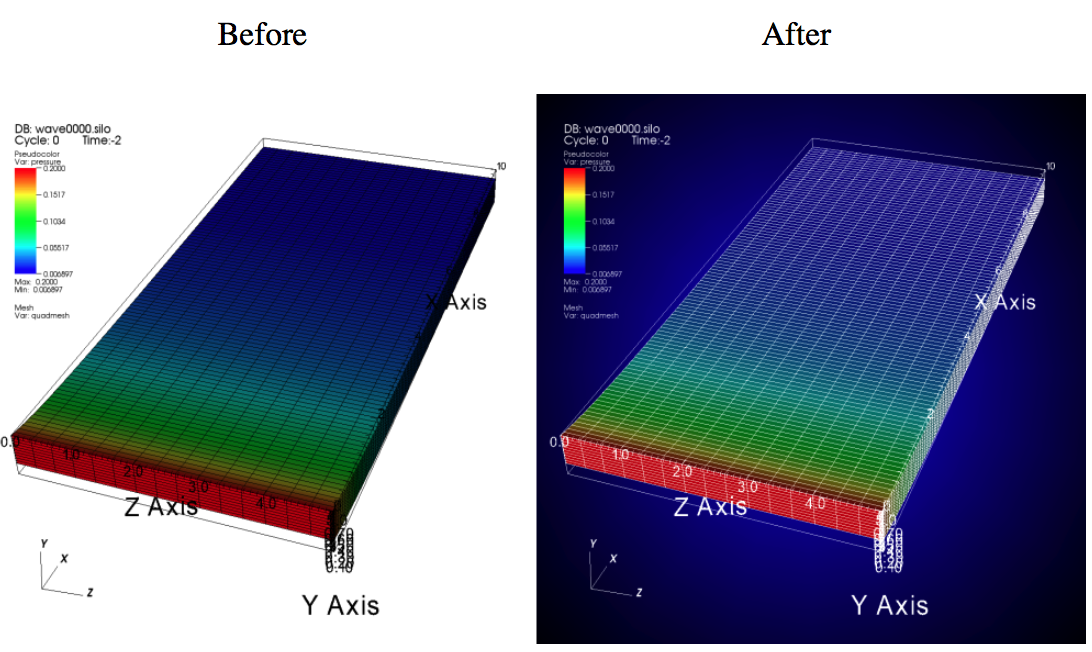
\includegraphics[width=5in]{annotation1.png}
\caption{Before and after image of adding a gradient background.}\end{figure}


\subsection{Adding a banner}
\label{quickrecipes:adding-a-banner}
Banners are useful for providing titles for a visualization or for
marking its content (see Figure
{\hyperref[quickrecipes:fig:annotations2]{\emph{{[}fig:annotations2{]}}}}). To add an ``Unclassified''
banner to a visualization, use the following bit of Python code:

\begin{Verbatim}[commandchars=\\\{\}]
\PYG{c+c1}{\PYGZsh{} Create a text object that we’ll use to indicate that our}
\PYG{c+c1}{\PYGZsh{} visualization is unclassified.}
\PYG{n}{banner} \PYG{o}{=} \PYG{n}{CreateAnnotationObject}\PYG{p}{(}\PYG{l+s+s2}{\PYGZdq{}}\PYG{l+s+s2}{Text2D}\PYG{l+s+s2}{\PYGZdq{}}\PYG{p}{)}
\PYG{n}{banner}\PYG{o}{.}\PYG{n}{text} \PYG{o}{=} \PYG{l+s+s2}{\PYGZdq{}}\PYG{l+s+s2}{Unclassified}\PYG{l+s+s2}{\PYGZdq{}}
\PYG{n}{banner}\PYG{o}{.}\PYG{n}{position} \PYG{o}{=} \PYG{p}{(}\PYG{l+m+mf}{0.37}\PYG{p}{,} \PYG{l+m+mf}{0.95}\PYG{p}{)}
\PYG{n}{banner}\PYG{o}{.}\PYG{n}{fontBold} \PYG{o}{=} \PYG{l+m+mi}{1}
\PYG{c+c1}{\PYGZsh{} print the attributes that you can set in the banner object.}
\PYG{k}{print} \PYG{n}{banner}
\end{Verbatim}
\centering\begin{figure}[htbp]
\centering
\capstart

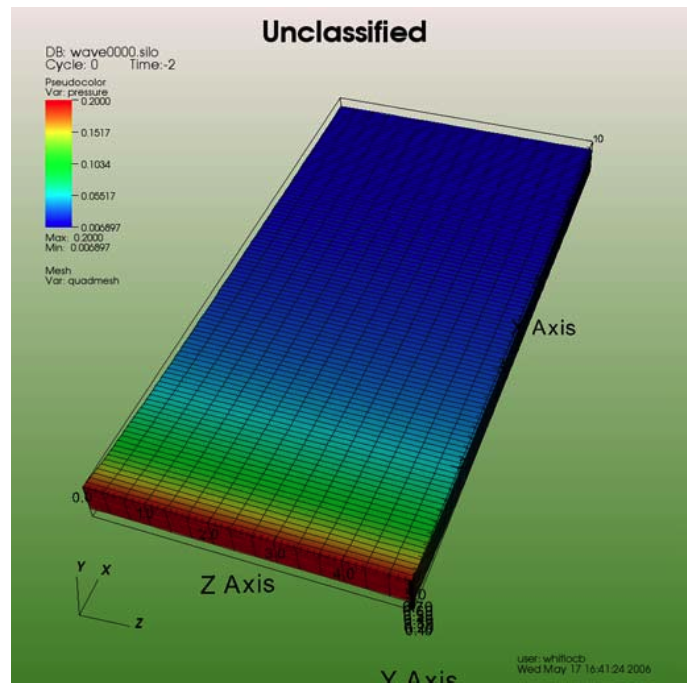
\includegraphics[width=3in]{annotation2.png}
\caption{Adding a banner}\end{figure}


\subsection{Adding a time slider}
\label{quickrecipes:adding-a-time-slider}
Time sliders are important annotations for movies since they convey how
much progress an animation has made as well as how many more frames have
yet to be seen. The time slider is also important for showing the
simulation time as the animation progresses so users can get a sense of
when in the simulation important events occur. VisIt’s time slider
annotation object is shown in Figure
{\hyperref[quickrecipes:fig:annotations3]{\emph{{[}fig:annotations3{]}}}}.

\begin{Verbatim}[commandchars=\\\{\}]
\PYG{c+c1}{\PYGZsh{} Add a time slider in the lower left corner}
\PYG{n}{slider} \PYG{o}{=} \PYG{n}{CreateAnnotationObject}\PYG{p}{(}\PYG{l+s+s2}{\PYGZdq{}}\PYG{l+s+s2}{TimeSlider}\PYG{l+s+s2}{\PYGZdq{}}\PYG{p}{)}
\PYG{n}{slider}\PYG{o}{.}\PYG{n}{height} \PYG{o}{=} \PYG{l+m+mf}{0.07}
\PYG{c+c1}{\PYGZsh{} Print the options that are available in the time slider object}
\PYG{k}{print} \PYG{n}{slider}
\end{Verbatim}
\centering\begin{figure}[htbp]
\centering
\capstart

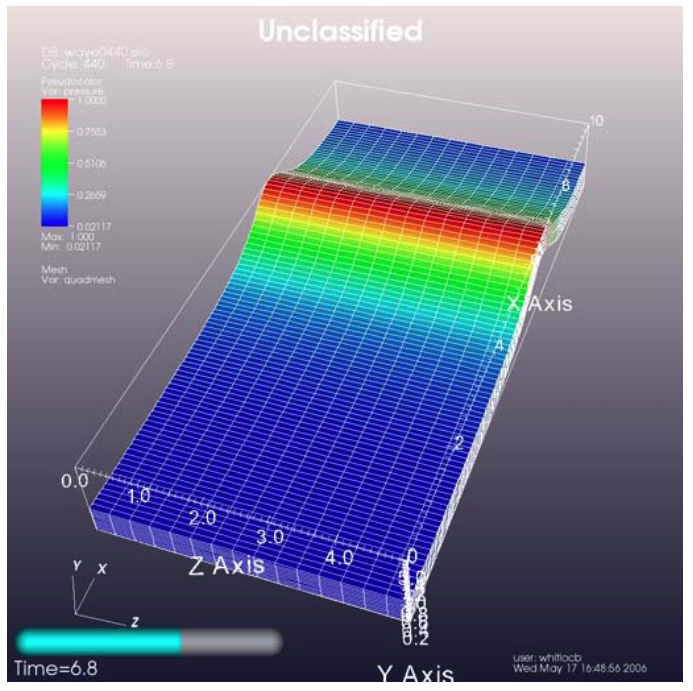
\includegraphics[width=3in]{annotation3.png}
\caption{Time slider annotation in the lower left corner}\end{figure}


\subsection{Adding a logo}
\label{quickrecipes:adding-a-logo}
Adding a logo to a visualization is an important part of project
identification for movies and other visualizations created with VisIt.
If you have a logo image file stored in TIFF, JPEG, BMP, or PPM format
then you can use it with VisIt as an image annotation (see Figure
{\hyperref[quickrecipes:fig:annotations4]{\emph{{[}fig:annotations4{]}}}}). Note that this approach can
also be used to insert images of graphs, plots, portraits, diagrams, or
any other form of image data into a visualization.

\begin{Verbatim}[commandchars=\\\{\}]
\PYG{c+c1}{\PYGZsh{} Incorporate LLNL logo image (llnl.jpeg) as an annotation}
\PYG{n}{image} \PYG{o}{=} \PYG{n}{CreateAnnotationObject}\PYG{p}{(}\PYG{l+s+s2}{\PYGZdq{}}\PYG{l+s+s2}{Image}\PYG{l+s+s2}{\PYGZdq{}}\PYG{p}{)}
\PYG{n}{image}\PYG{o}{.}\PYG{n}{image} \PYG{o}{=} \PYG{l+s+s2}{\PYGZdq{}}\PYG{l+s+s2}{llnl.jpeg}\PYG{l+s+s2}{\PYGZdq{}}
\PYG{n}{image}\PYG{o}{.}\PYG{n}{position} \PYG{o}{=} \PYG{p}{(}\PYG{l+m+mf}{0.02}\PYG{p}{,} \PYG{l+m+mf}{0.02}\PYG{p}{)}
\PYG{c+c1}{\PYGZsh{} Print the other image annotation options}
\PYG{k}{print} \PYG{n}{image}
\end{Verbatim}
\centering\begin{figure}[htbp]
\centering
\capstart

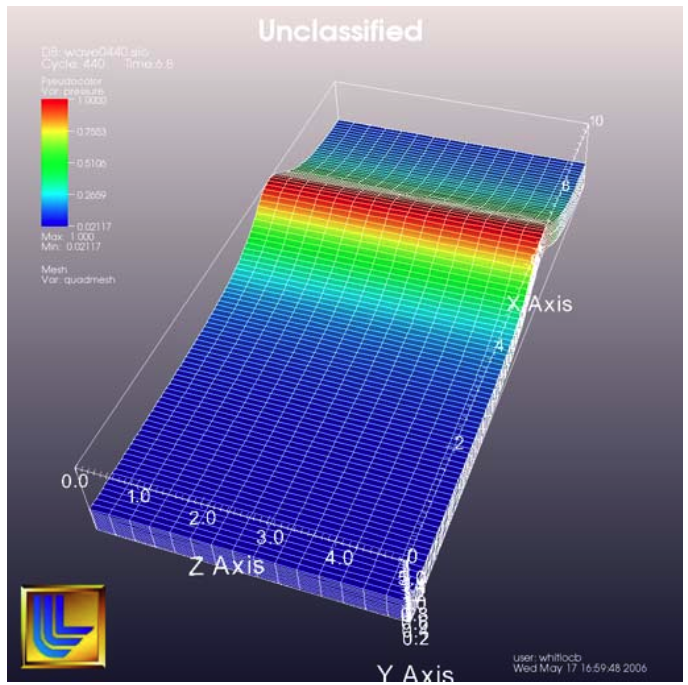
\includegraphics[width=3in]{annotation4.png}
\caption{Image annotation used to incorporate LLNL logo}\end{figure}


\chapter{Functions}
\label{functions::doc}\label{functions:functions}\label{functions:visit}
\begin{DUlineblock}{0em}
\item[] 
\item[] 
\end{DUlineblock}


\section{ActivateDatabase}
\label{functions:activatedatabase}
\begin{DUlineblock}{0em}
\item[] \textbf{Synopsis:}
\end{DUlineblock}
\begin{quote}

\begin{tabulary}{\linewidth}{|L|}
\hline

ActivateDatabase(argument) -\textgreater{} integer
\\
\hline\end{tabulary}

\end{quote}

\begin{DUlineblock}{0em}
\item[] 
\item[] \textbf{Arguments:}
\end{DUlineblock}
\begin{quote}

\begin{tabular}{|p{0.475\linewidth}|p{0.475\linewidth}|}
\hline

argument
 & 
\begin{DUlineblock}{0em}
\item[] A string object containing the name of the database to
\item[] be activated.
\end{DUlineblock}
\\
\hline\end{tabular}

\end{quote}

\begin{DUlineblock}{0em}
\item[] 
\item[] \textbf{Returns:}
\item[] ActivateDatabase returns 1 on success and 0 on failure.
\item[] 
\item[] \textbf{Description:}
\item[] The ActivateDatabase function is used to set the active database to a
database that has been previously opened. The ActivateDatabase function
only works when you are using it to activate a database that you have
previously opened. You do not need to use this function unless you
frequently toggle between more than one database when making plots or
changing time states. While the OpenDatabase function can also be used
to set the active database, the ActivateDatabase function does not have any
side effects that would cause the time state for the new active database
to be changed.
\end{DUlineblock}

\begin{DUlineblock}{0em}
\item[] 
\end{DUlineblock}

\begin{DUlineblock}{0em}
\item[] \textbf{Example:}
\item[] 
\end{DUlineblock}
\begin{quote}

\begin{Verbatim}[commandchars=\\\{\}]
\PYG{c+c1}{\PYGZsh{}\PYGZpc{} visit \PYGZhy{}cli}
\PYG{n}{dbs} \PYG{o}{=} \PYG{p}{(}\PYG{l+s+s2}{\PYGZdq{}}\PYG{l+s+s2}{/usr/gapps/visit/data/wave.visit}\PYG{l+s+s2}{\PYGZdq{}}\PYG{p}{,} \PYGZbs{}
\PYG{l+s+s2}{\PYGZdq{}}\PYG{l+s+s2}{/usr/gapps/visit/data/curv3d.silo}\PYG{l+s+s2}{\PYGZdq{}}\PYG{p}{)}
\PYG{n}{OpenDatabase}\PYG{p}{(}\PYG{n}{dbs}\PYG{p}{[}\PYG{l+m+mi}{0}\PYG{p}{]}\PYG{p}{,} \PYG{l+m+mi}{17}\PYG{p}{)}
\PYG{n}{AddPlot}\PYG{p}{(}\PYG{l+s+s2}{\PYGZdq{}}\PYG{l+s+s2}{Pseudocolor}\PYG{l+s+s2}{\PYGZdq{}}\PYG{p}{,} \PYG{l+s+s2}{\PYGZdq{}}\PYG{l+s+s2}{u}\PYG{l+s+s2}{\PYGZdq{}}\PYG{p}{)}
\PYG{n}{DrawPlots}\PYG{p}{(}\PYG{p}{)}
\PYG{n}{OpenDatabase}\PYG{p}{(}\PYG{n}{dbs}\PYG{p}{[}\PYG{l+m+mi}{1}\PYG{p}{]}\PYG{p}{)}
\PYG{n}{AddPlot}\PYG{p}{(}\PYG{l+s+s2}{\PYGZdq{}}\PYG{l+s+s2}{Pseudocolor}\PYG{l+s+s2}{\PYGZdq{}}\PYG{p}{,} \PYG{l+s+s2}{\PYGZdq{}}\PYG{l+s+s2}{u}\PYG{l+s+s2}{\PYGZdq{}}\PYG{p}{)}
\PYG{n}{DrawPlots}\PYG{p}{(}\PYG{p}{)}
\PYG{c+c1}{\PYGZsh{} Let\PYGZsq{}s add another plot from the first database.}
\PYG{n}{ActivateDatabase}\PYG{p}{(}\PYG{n}{dbs}\PYG{p}{[}\PYG{l+m+mi}{0}\PYG{p}{]}\PYG{p}{)}
\PYG{n}{AddPlot}\PYG{p}{(}\PYG{l+s+s2}{\PYGZdq{}}\PYG{l+s+s2}{Mesh}\PYG{l+s+s2}{\PYGZdq{}}\PYG{p}{,} \PYG{l+s+s2}{\PYGZdq{}}\PYG{l+s+s2}{quadmesh}\PYG{l+s+s2}{\PYGZdq{}}\PYG{p}{)}
\PYG{n}{DrawPlots}\PYG{p}{(}\PYG{p}{)}
\end{Verbatim}
\end{quote}


\section{AddArgument}
\label{functions:addargument}
\begin{DUlineblock}{0em}
\item[] \textbf{Synopsis:}
\end{DUlineblock}
\begin{quote}

\begin{tabulary}{\linewidth}{|L|}
\hline

AddArgument(argument)
\\
\hline\end{tabulary}

\end{quote}

\begin{DUlineblock}{0em}
\item[] 
\item[] \textbf{Arguments:}
\end{DUlineblock}
\begin{quote}

\begin{tabular}{|p{0.475\linewidth}|p{0.475\linewidth}|}
\hline

argument
 & 
\begin{DUlineblock}{0em}
\item[] A string object that is added to the viewer's command
\item[] line argument list.
\end{DUlineblock}
\\
\hline\end{tabular}

\end{quote}

\begin{DUlineblock}{0em}
\item[] 
\item[] \textbf{Returns:}
\item[] AddArgument does not return a value.
\item[] 
\item[] \textbf{Description:}
\item[] The AddArgument function is used to add extra command line arguments to
VisIt's viewer. This is only useful when VisIt's Python interface is
imported into a stand-alone Python interpreter because the AddArgument
function must be called before the viewer is launched. The AddArgument
function has no effect when used in VisIt's cli program because the viewer
is automatically launched before any commands are processed.
\end{DUlineblock}

\begin{DUlineblock}{0em}
\item[] 
\end{DUlineblock}

\begin{DUlineblock}{0em}
\item[] \textbf{Example:}
\item[] 
\end{DUlineblock}
\begin{quote}

\begin{Verbatim}[commandchars=\\\{\}]
\PYG{k+kn}{import} \PYG{n+nn}{visit}
\PYG{n}{visit}\PYG{o}{.}\PYG{n}{AddArgument}\PYG{p}{(}\PYG{l+s+s2}{\PYGZdq{}}\PYG{l+s+s2}{\PYGZhy{}nowin}\PYG{l+s+s2}{\PYGZdq{}}\PYG{p}{)} \PYG{c+c1}{\PYGZsh{} Add the \PYGZhy{}nowin argument to the viewer.}
\end{Verbatim}
\end{quote}


\section{AddMachineProfile}
\label{functions:addmachineprofile}
\begin{DUlineblock}{0em}
\item[] \textbf{Synopsis:}
\end{DUlineblock}
\begin{quote}

\begin{tabulary}{\linewidth}{|L|}
\hline

AddMachineProfile(MachineProfile) -\textgreater{} integer
\\
\hline\end{tabulary}

\end{quote}

\begin{DUlineblock}{0em}
\item[] 
\item[] \textbf{Arguments:}
\end{DUlineblock}
\begin{quote}

\begin{tabulary}{\linewidth}{|L|L|}
\hline

MachineProfile
 & \\
\hline\end{tabulary}

\end{quote}

\begin{DUlineblock}{0em}
\item[] 
\item[] \textbf{Description:}
\item[] Sets the input machine profile in the HostProfileList, replaces if one already exists
Otherwise adds to the list
\end{DUlineblock}

\begin{DUlineblock}{0em}
\item[] 
\end{DUlineblock}


\section{AddOperator}
\label{functions:addoperator}
\begin{DUlineblock}{0em}
\item[] \textbf{Synopsis:}
\end{DUlineblock}
\begin{quote}

\begin{tabulary}{\linewidth}{|L|}
\hline

AddOperator(operator) -\textgreater{} integer
\\
\hline
AddOperator(operator, all) -\textgreater{} integer
\\
\hline\end{tabulary}

\end{quote}

\begin{DUlineblock}{0em}
\item[] 
\item[] \textbf{Arguments:}
\end{DUlineblock}
\begin{quote}

\begin{tabular}{|p{0.475\linewidth}|p{0.475\linewidth}|}
\hline

operator
 & 
\begin{DUlineblock}{0em}
\item[] This is a string containing the name of the operator to
\item[] be applied.
\end{DUlineblock}
\\
\hline
all
 & 
\begin{DUlineblock}{0em}
\item[] This is an optional integer argument that applies the
\item[] operator to all plots if the value of the argument is
\item[] not zero.
\end{DUlineblock}
\\
\hline\end{tabular}

\end{quote}

\begin{DUlineblock}{0em}
\item[] 
\item[] \textbf{Returns:}
\item[] The AddOperator function returns an integer value of 1 for success and 0
\item[] for failure.
\item[] 
\item[] \textbf{Description:}
\item[] The AddOperator function adds a VisIt operator to the active plots. The
operator argument is a string containing the name of the operator to be
added to the active plots. The operatore name must be a valid operator
plugin name that is a member of the tuple returned by the OperatorPlugins
function. The all argument is an integer that determines
whether or not the operator is applied to all plots. If the all argument is
not provided, the operator is only added to active plots. Once the
AddOperator function is called, the desired operator is added to all
active plots unless the all argument is a non-zero value. When the all
argument is a non-zero value, the operator is applied to all plots
regardless of whether or not they are selected. Operator attributes are set
through the SetOperatorOptions function.
\end{DUlineblock}

\begin{DUlineblock}{0em}
\item[] 
\end{DUlineblock}

\begin{DUlineblock}{0em}
\item[] \textbf{Example:}
\item[] 
\end{DUlineblock}
\begin{quote}

\begin{Verbatim}[commandchars=\\\{\}]
\PYG{c+c1}{\PYGZsh{}\PYGZpc{} visit \PYGZhy{}cli}
\PYG{n}{OpenDatabase}\PYG{p}{(}\PYG{l+s+s2}{\PYGZdq{}}\PYG{l+s+s2}{/usr/gapps/visit/data/globe.silo}\PYG{l+s+s2}{\PYGZdq{}}\PYG{p}{)}
\PYG{n}{AddPlot}\PYG{p}{(}\PYG{l+s+s2}{\PYGZdq{}}\PYG{l+s+s2}{Pseudocolor}\PYG{l+s+s2}{\PYGZdq{}}\PYG{p}{,} \PYG{l+s+s2}{\PYGZdq{}}\PYG{l+s+s2}{u}\PYG{l+s+s2}{\PYGZdq{}}\PYG{p}{)}
\PYG{n}{AddPlot}\PYG{p}{(}\PYG{l+s+s2}{\PYGZdq{}}\PYG{l+s+s2}{Mesh}\PYG{l+s+s2}{\PYGZdq{}}\PYG{p}{,} \PYG{l+s+s2}{\PYGZdq{}}\PYG{l+s+s2}{mesh1}\PYG{l+s+s2}{\PYGZdq{}}\PYG{p}{)}
\PYG{n}{AddOperator}\PYG{p}{(}\PYG{l+s+s2}{\PYGZdq{}}\PYG{l+s+s2}{Slice}\PYG{l+s+s2}{\PYGZdq{}}\PYG{p}{,} \PYG{l+m+mi}{1}\PYG{p}{)} \PYG{c+c1}{\PYGZsh{} Slice both plots}
\PYG{n}{DrawPlots}\PYG{p}{(}\PYG{p}{)}
\end{Verbatim}
\end{quote}


\section{AddPlot}
\label{functions:addplot}
\begin{DUlineblock}{0em}
\item[] \textbf{Synopsis:}
\end{DUlineblock}
\begin{quote}

\begin{tabulary}{\linewidth}{|L|}
\hline

AddPlot(plotType, variableName) -\textgreater{} integer
\\
\hline
AddPlot(plotType, variableName, inheritSIL) -\textgreater{} integer
\\
\hline
AddPlot(plotType, variableName, inheritSIL, applyOperators) -\textgreater{} integer
\\
\hline\end{tabulary}

\end{quote}

\begin{DUlineblock}{0em}
\item[] 
\item[] \textbf{Arguments:}
\end{DUlineblock}
\begin{quote}

\begin{tabular}{|p{0.475\linewidth}|p{0.475\linewidth}|}
\hline

plotType
 & 
\begin{DUlineblock}{0em}
\item[] This is a string containing the name of a valid plot
\item[] plugin type.
\end{DUlineblock}
\\
\hline
variableName
 & 
\begin{DUlineblock}{0em}
\item[] This is a string containing a valid variable name for
\item[] the open database.
\end{DUlineblock}
\\
\hline
inheritSIL
 & 
\begin{DUlineblock}{0em}
\item[] This is an integer flag indicating whether the plot
\item[] should inherit theactive plot's SIL restriction.
\end{DUlineblock}
\\
\hline
applyOperators
 & 
\begin{DUlineblock}{0em}
\item[] This is an integer flag indicating whether the
\item[] operators from the active plot should be applied to
\item[] the new plot.
\end{DUlineblock}
\\
\hline\end{tabular}

\end{quote}

\begin{DUlineblock}{0em}
\item[] 
\item[] \textbf{Returns:}
\item[] The AddPlot function returns an integer value of 1 for success and 0 for
\item[] failure.
\item[] 
\item[] \textbf{Description:}
\item[] The AddPlot function creates a new plot of the specified type using a
variable from the open database. The plotType argument is a string that
contains the name of a valid plot plugin type which must be a member of the
string tuple that is returned by the PlotPlugins function.
The variableName argument is a string that contains the name of a variable
in the open database. After the AddPlot function is called, a new plot is
created and it is made the sole active plot.
\end{DUlineblock}

\begin{DUlineblock}{0em}
\item[] 
\end{DUlineblock}

\begin{DUlineblock}{0em}
\item[] \textbf{Example:}
\item[] 
\end{DUlineblock}
\begin{quote}

\begin{Verbatim}[commandchars=\\\{\}]
\PYG{c+c1}{\PYGZsh{}\PYGZpc{} visit \PYGZhy{}cli}
\PYG{n}{OpenDatabase}\PYG{p}{(}\PYG{l+s+s2}{\PYGZdq{}}\PYG{l+s+s2}{/usr/gapps/visit/data/globe.silo}\PYG{l+s+s2}{\PYGZdq{}}\PYG{p}{)}
\PYG{n}{AddPlot}\PYG{p}{(}\PYG{l+s+s2}{\PYGZdq{}}\PYG{l+s+s2}{Subset}\PYG{l+s+s2}{\PYGZdq{}}\PYG{p}{,} \PYG{l+s+s2}{\PYGZdq{}}\PYG{l+s+s2}{mat1}\PYG{l+s+s2}{\PYGZdq{}}\PYG{p}{)} \PYG{c+c1}{\PYGZsh{} Create a subset plot}
\PYG{n}{DrawPlots}\PYG{p}{(}\PYG{p}{)}
\end{Verbatim}
\end{quote}


\section{AddWindow}
\label{functions:addwindow}
\begin{DUlineblock}{0em}
\item[] \textbf{Synopsis:}
\end{DUlineblock}
\begin{quote}

\begin{tabulary}{\linewidth}{|L|}
\hline

AddWindow()
\\
\hline\end{tabulary}

\end{quote}

\begin{DUlineblock}{0em}
\item[] 
\item[] \textbf{Returns:}
\item[] The AddWindow function does not a return value.
\item[] 
\item[] \textbf{Description:}
\item[] The AddWindow function creates a new visualization window and makes it the
active window. This function can be used to create up to 16 visualization
windows. After that, the AddWindow function has no effect.
\end{DUlineblock}

\begin{DUlineblock}{0em}
\item[] 
\end{DUlineblock}

\begin{DUlineblock}{0em}
\item[] \textbf{Example:}
\item[] 
\end{DUlineblock}
\begin{quote}

\begin{Verbatim}[commandchars=\\\{\}]
\PYG{k+kn}{import} \PYG{n+nn}{visit}
\PYG{n}{visit}\PYG{o}{.}\PYG{n}{Launch}\PYG{p}{(}\PYG{p}{)}
\PYG{n}{visit}\PYG{o}{.}\PYG{n}{AddWindow}\PYG{p}{(}\PYG{p}{)} \PYG{c+c1}{\PYGZsh{} Create window \PYGZsh{}2}
\PYG{n}{visit}\PYG{o}{.}\PYG{n}{AddWindow}\PYG{p}{(}\PYG{p}{)} \PYG{c+c1}{\PYGZsh{} Create window \PYGZsh{}3}
\end{Verbatim}
\end{quote}


\section{AlterDatabaseCorrelation}
\label{functions:alterdatabasecorrelation}
\begin{DUlineblock}{0em}
\item[] \textbf{Synopsis:}
\end{DUlineblock}
\begin{quote}

\begin{tabulary}{\linewidth}{|L|}
\hline

AlterDatabaseCorrelation(name, databases, method) -\textgreater{} integer
\\
\hline\end{tabulary}

\end{quote}

\begin{DUlineblock}{0em}
\item[] 
\item[] \textbf{Arguments:}
\end{DUlineblock}
\begin{quote}

\begin{tabular}{|p{0.475\linewidth}|p{0.475\linewidth}|}
\hline

name
 & 
\begin{DUlineblock}{0em}
\item[] The name argument must be a string object containing
\item[] the name of the database correlation to be altered.
\end{DUlineblock}
\\
\hline
databases
 & 
\begin{DUlineblock}{0em}
\item[] The databases argument must be a tuple or list of
\item[] strings containing the fully qualified database
\item[] names to be used in the database correlation.
\end{DUlineblock}
\\
\hline
method
 & 
\begin{DUlineblock}{0em}
\item[] The method argument must be an integer in the range
\item[] {[}0,3{]}.
\end{DUlineblock}
\\
\hline\end{tabular}

\end{quote}

\begin{DUlineblock}{0em}
\item[] 
\item[] \textbf{Returns:}
\item[] The AlterDatabaseCorrelation function returns 1 on success and 0 on
\item[] failure.
\item[] 
\item[] \textbf{Description:}
\item[] The AlterDatabaseCorrelation method alters an existing database
correlation. A database correlation is a VisIt construct that relates the
time states for two or more databases in some way. You would use the
AlterDatabaseCorrelation function if you wanted to change the list of
databases used in a database correlation or if you wanted to change how the
databases are related - the correlation method. The name argument is a
string that is the name of the database correlation to be altered. If the
name that you pass is not a valid database correlation then the
AlterDatabaseCorrelation function fails. The databases argument is a list
or tuple of string objects containing the fully-qualified
(host:/path/filename) names of the databases to be involved in the database
query. The method argument allows you to specify a database correlation
method.
\item[] 
\end{DUlineblock}
\begin{quote}

\begin{tabulary}{\linewidth}{|L|L|}
\hline

\textbf{Correlation method}
 & 
Value
\\
\hline
IndexForIndexCorrelation
 & 
0
\\
\hline
StretchedIndexCorrelation
 & 
1
\\
\hline
TimeCorrelation
 & 
2
\\
\hline
CycleCorrelation
 & 
3
\\
\hline\end{tabulary}

\end{quote}

\begin{DUlineblock}{0em}
\item[] 
\end{DUlineblock}

\begin{DUlineblock}{0em}
\item[] \textbf{Example:}
\item[] 
\end{DUlineblock}
\begin{quote}

\begin{Verbatim}[commandchars=\\\{\}]
\PYG{n}{dbs} \PYG{o}{=} \PYG{p}{(}\PYG{l+s+s2}{\PYGZdq{}}\PYG{l+s+s2}{/usr/gapps/visit/data/wave.visit}\PYG{l+s+s2}{\PYGZdq{}}\PYG{p}{,} \PYGZbs{}
\PYG{l+s+s2}{\PYGZdq{}}\PYG{l+s+s2}{/usr/gapps/visit/data/wave*.silo database}\PYG{l+s+s2}{\PYGZdq{}}\PYG{p}{)}
\PYG{n}{OpenDatabase}\PYG{p}{(}\PYG{n}{dbs}\PYG{p}{[}\PYG{l+m+mi}{0}\PYG{p}{]}\PYG{p}{)}
\PYG{n}{AddPlot}\PYG{p}{(}\PYG{l+s+s2}{\PYGZdq{}}\PYG{l+s+s2}{Pseudocolor}\PYG{l+s+s2}{\PYGZdq{}}\PYG{p}{,} \PYG{l+s+s2}{\PYGZdq{}}\PYG{l+s+s2}{pressure}\PYG{l+s+s2}{\PYGZdq{}}\PYG{p}{)}
\PYG{n}{OpenDatabase}\PYG{p}{(}\PYG{n}{dbs}\PYG{p}{[}\PYG{l+m+mi}{1}\PYG{p}{]}\PYG{p}{)}
\PYG{n}{AddPlot}\PYG{p}{(}\PYG{l+s+s2}{\PYGZdq{}}\PYG{l+s+s2}{Pseudocolor}\PYG{l+s+s2}{\PYGZdq{}}\PYG{p}{,} \PYG{l+s+s2}{\PYGZdq{}}\PYG{l+s+s2}{d}\PYG{l+s+s2}{\PYGZdq{}}\PYG{p}{)}
\PYG{c+c1}{\PYGZsh{} VisIt created an index for index database correlation but we}
\PYG{c+c1}{\PYGZsh{} want a cycle correlation.}
\PYG{n}{AlterDatabaseCorrelation}\PYG{p}{(}\PYG{l+s+s2}{\PYGZdq{}}\PYG{l+s+s2}{Correlation01}\PYG{l+s+s2}{\PYGZdq{}}\PYG{p}{,} \PYG{n}{dbs}\PYG{p}{,} \PYG{l+m+mi}{3}\PYG{p}{)}
\end{Verbatim}
\end{quote}


\section{ApplyNamedSelection}
\label{functions:applynamedselection}
\begin{DUlineblock}{0em}
\item[] \textbf{Synopsis:}
\end{DUlineblock}
\begin{quote}

\begin{tabulary}{\linewidth}{|L|}
\hline

ApplyNamedSelection(name) -\textgreater{} integer
\\
\hline\end{tabulary}

\end{quote}

\begin{DUlineblock}{0em}
\item[] 
\item[] \textbf{Arguments:}
\end{DUlineblock}
\begin{quote}

\begin{tabular}{|p{0.475\linewidth}|p{0.475\linewidth}|}
\hline

name
 & 
\begin{DUlineblock}{0em}
\item[] The name of a named selection. (This should have been
\item[] previously createdwith a CreateNamedSelection
\item[] call.)
\end{DUlineblock}
\\
\hline\end{tabular}

\end{quote}

\begin{DUlineblock}{0em}
\item[] 
\item[] \textbf{Returns:}
\item[] The ApplyNamedSelection function returns 1 for success and 0 for failure.
\item[] 
\item[] \textbf{Description:}
\item[] Named Selections allow you to select a group of elements (or particles).
One typically creates a named selection from a group of elements and then
later applies the named selection to another plot (thus reducing the
set of elements displayed to the ones from when the named selection was
created).
\end{DUlineblock}

\begin{DUlineblock}{0em}
\item[] 
\end{DUlineblock}

\begin{DUlineblock}{0em}
\item[] \textbf{Example:}
\item[] 
\end{DUlineblock}
\begin{quote}

\begin{Verbatim}[commandchars=\\\{\}]
\PYG{c+c1}{\PYGZsh{}\PYGZpc{} visit \PYGZhy{}cli}
\PYG{n}{db} \PYG{o}{=} \PYG{l+s+s2}{\PYGZdq{}}\PYG{l+s+s2}{/usr/gapps/visit/data/wave*.silo database}\PYG{l+s+s2}{\PYGZdq{}}
\PYG{n}{OpenDatabase}\PYG{p}{(}\PYG{n}{db}\PYG{p}{)}
\PYG{n}{AddPlot}\PYG{p}{(}\PYG{l+s+s2}{\PYGZdq{}}\PYG{l+s+s2}{Pseudocolor}\PYG{l+s+s2}{\PYGZdq{}}\PYG{p}{,} \PYG{l+s+s2}{\PYGZdq{}}\PYG{l+s+s2}{pressure}\PYG{l+s+s2}{\PYGZdq{}}\PYG{p}{)}
\PYG{n}{AddOperator}\PYG{p}{(}\PYG{l+s+s2}{\PYGZdq{}}\PYG{l+s+s2}{Clip}\PYG{l+s+s2}{\PYGZdq{}}\PYG{p}{)}
\PYG{n}{c} \PYG{o}{=} \PYG{n}{ClipAttributes}\PYG{p}{(}\PYG{p}{)}
\PYG{n}{c}\PYG{o}{.}\PYG{n}{plane1Origin} \PYG{o}{=} \PYG{p}{(}\PYG{l+m+mi}{0}\PYG{p}{,}\PYG{l+m+mf}{0.6}\PYG{p}{,}\PYG{l+m+mi}{0}\PYG{p}{)}
\PYG{n}{c}\PYG{o}{.}\PYG{n}{plane1Normal} \PYG{o}{=} \PYG{p}{(}\PYG{l+m+mi}{0}\PYG{p}{,}\PYG{o}{\PYGZhy{}}\PYG{l+m+mi}{1}\PYG{p}{,}\PYG{l+m+mi}{0}\PYG{p}{)}
\PYG{n}{SetOperatorOption}\PYG{p}{(}\PYG{n}{c}\PYG{p}{)}
\PYG{n}{DrawPlots}\PYG{p}{(}\PYG{p}{)}
\PYG{n}{CreateNamedSelection}\PYG{p}{(}\PYG{l+s+s2}{\PYGZdq{}}\PYG{l+s+s2}{els\PYGZus{}above\PYGZus{}at\PYGZus{}time\PYGZus{}0}\PYG{l+s+s2}{\PYGZdq{}}\PYG{p}{)}
\PYG{n}{SetTimeSliderState}\PYG{p}{(}\PYG{l+m+mi}{40}\PYG{p}{)}
\PYG{n}{RemoveLastOperator}\PYG{p}{(}\PYG{p}{)}
\PYG{n}{ApplyNamedSelection}\PYG{p}{(}\PYG{l+s+s2}{\PYGZdq{}}\PYG{l+s+s2}{els\PYGZus{}above\PYGZus{}at\PYGZus{}time\PYGZus{}0}\PYG{l+s+s2}{\PYGZdq{}}\PYG{p}{)}
\end{Verbatim}
\end{quote}


\section{ChangeActivePlotsVar}
\label{functions:changeactiveplotsvar}
\begin{DUlineblock}{0em}
\item[] \textbf{Synopsis:}
\end{DUlineblock}
\begin{quote}

\begin{tabulary}{\linewidth}{|L|}
\hline

ChangeActivePlotsVar(variableName) -\textgreater{} integer
\\
\hline\end{tabulary}

\end{quote}

\begin{DUlineblock}{0em}
\item[] 
\item[] \textbf{Arguments:}
\end{DUlineblock}
\begin{quote}

\begin{tabulary}{\linewidth}{|L|L|}
\hline

variableName
 & 
The name of the new plot variable.
\\
\hline\end{tabulary}

\end{quote}

\begin{DUlineblock}{0em}
\item[] 
\item[] \textbf{Returns:}
\item[] The ChangeActivePlotsVar function returns an integer value of 1 for
\item[] success and 0 for failure.
\item[] 
\item[] \textbf{Description:}
\item[] The ChangeActivePlotsVar function changes the plotted variable for the
active plots. This is a useful way to change what is being visualized
without having to delete and recreate the current plots. The variableName
argument is a string that contains the name of a variable in the open
database.
\end{DUlineblock}

\begin{DUlineblock}{0em}
\item[] 
\end{DUlineblock}

\begin{DUlineblock}{0em}
\item[] \textbf{Example:}
\item[] 
\end{DUlineblock}
\begin{quote}

\begin{Verbatim}[commandchars=\\\{\}]
\PYG{c+c1}{\PYGZsh{}\PYGZpc{} visit \PYGZhy{}cli}
\PYG{n}{OpenDatabase}\PYG{p}{(}\PYG{l+s+s2}{\PYGZdq{}}\PYG{l+s+s2}{/usr/gapps/visit/data/globe.silo}\PYG{l+s+s2}{\PYGZdq{}}\PYG{p}{)}
\PYG{n}{AddPlot}\PYG{p}{(}\PYG{l+s+s2}{\PYGZdq{}}\PYG{l+s+s2}{Pseudocolor}\PYG{l+s+s2}{\PYGZdq{}}\PYG{p}{,} \PYG{l+s+s2}{\PYGZdq{}}\PYG{l+s+s2}{u}\PYG{l+s+s2}{\PYGZdq{}}\PYG{p}{)}
\PYG{n}{DrawPlots}\PYG{p}{(}\PYG{p}{)}
\PYG{n}{SaveWindow}\PYG{p}{(}\PYG{p}{)}
\PYG{n}{ChangeActivePlotsVar}\PYG{p}{(}\PYG{l+s+s2}{\PYGZdq{}}\PYG{l+s+s2}{v}\PYG{l+s+s2}{\PYGZdq{}}\PYG{p}{)}
\end{Verbatim}
\end{quote}


\section{CheckForNewStates}
\label{functions:checkfornewstates}
\begin{DUlineblock}{0em}
\item[] \textbf{Synopsis:}
\end{DUlineblock}
\begin{quote}

\begin{tabulary}{\linewidth}{|L|}
\hline

CheckForNewStates(name) -\textgreater{} integer
\\
\hline\end{tabulary}

\end{quote}

\begin{DUlineblock}{0em}
\item[] 
\item[] \textbf{Arguments:}
\end{DUlineblock}
\begin{quote}

\begin{tabular}{|p{0.475\linewidth}|p{0.475\linewidth}|}
\hline

name
 & 
\begin{DUlineblock}{0em}
\item[] The name argument must be a string that contains the
\item[] name of a database that has been opened previously.
\end{DUlineblock}
\\
\hline\end{tabular}

\end{quote}

\begin{DUlineblock}{0em}
\item[] 
\item[] \textbf{Returns:}
\item[] The CheckForNewStates function returns 1 for success and 0 for failure.
\item[] 
\item[] \textbf{Description:}
\item[] Calculations are often run at the same time as some of the preliminary
visualization work is being performed. That said, you might be visualizing
the leading time states of a database that is still being created. If you
want to force VisIt to add any new time states that were added since you
opened the database, you can use the CheckForNewStates function. The name
argument must contain the name of a database that has been opened before.
\end{DUlineblock}

\begin{DUlineblock}{0em}
\item[] 
\end{DUlineblock}

\begin{DUlineblock}{0em}
\item[] \textbf{Example:}
\item[] 
\end{DUlineblock}
\begin{quote}

\begin{Verbatim}[commandchars=\\\{\}]
\PYG{c+c1}{\PYGZsh{}\PYGZpc{} visit \PYGZhy{}cli}
\PYG{n}{db} \PYG{o}{=} \PYG{l+s+s2}{\PYGZdq{}}\PYG{l+s+s2}{/usr/gapps/visit/data/wave*.silo database}\PYG{l+s+s2}{\PYGZdq{}}
\PYG{n}{OpenDatabase}\PYG{p}{(}\PYG{n}{db}\PYG{p}{)}
\PYG{n}{AddPlot}\PYG{p}{(}\PYG{l+s+s2}{\PYGZdq{}}\PYG{l+s+s2}{Pseudocolor}\PYG{l+s+s2}{\PYGZdq{}}\PYG{p}{,} \PYG{l+s+s2}{\PYGZdq{}}\PYG{l+s+s2}{pressure}\PYG{l+s+s2}{\PYGZdq{}}\PYG{p}{)}
\PYG{n}{DrawPlots}\PYG{p}{(}\PYG{p}{)}
\PYG{n}{SetTimeSliderState}\PYG{p}{(}\PYG{n}{TimeSliderGetNStates}\PYG{p}{(}\PYG{p}{)} \PYG{o}{\PYGZhy{}} \PYG{l+m+mi}{1}\PYG{p}{)}
\PYG{c+c1}{\PYGZsh{} More files appear on disk}
\PYG{n}{CheckForNewStates}\PYG{p}{(}\PYG{n}{db}\PYG{p}{)}
\PYG{n}{SetTimeSliderState}\PYG{p}{(}\PYG{n}{TimeSliderGetNStates}\PYG{p}{(}\PYG{p}{)} \PYG{o}{\PYGZhy{}} \PYG{l+m+mi}{1}\PYG{p}{)}
\end{Verbatim}
\end{quote}


\section{ChooseCenterOfRotation}
\label{functions:choosecenterofrotation}
\begin{DUlineblock}{0em}
\item[] \textbf{Synopsis:}
\end{DUlineblock}
\begin{quote}

\begin{tabulary}{\linewidth}{|L|}
\hline

ChooseCenterOfRotation() -\textgreater{} integer
\\
\hline
ChooseCenterOfRotation(screenX, screenY) -\textgreater{} integer
\\
\hline\end{tabulary}

\end{quote}

\begin{DUlineblock}{0em}
\item[] 
\item[] \textbf{Arguments:}
\end{DUlineblock}
\begin{quote}

\begin{tabular}{|p{0.475\linewidth}|p{0.475\linewidth}|}
\hline

screenX
 & 
\begin{DUlineblock}{0em}
\item[] The X coordinate of the pick point in normalized {[}0,1{]}
\item[] screen space.
\end{DUlineblock}
\\
\hline
screenY
 & 
\begin{DUlineblock}{0em}
\item[] The Y cooridinate of the pick point in normalized
\item[] {[}0,1{]} screen space.
\end{DUlineblock}
\\
\hline\end{tabular}

\end{quote}

\begin{DUlineblock}{0em}
\item[] 
\item[] \textbf{Returns:}
\item[] The ChooseCenterOfRotation function returns 1 if successful and 0 if it
\item[] fails.
\item[] 
\item[] \textbf{Description:}
\item[] The ChooseCenterOfRotation function allows you to pick a new center of
rotation, which is the point about which plots are rotated when you
interactively rotate plots. The function can either take zero arguments, in
which case you must interactively pick on plots, or it can take two
arguments that correspond to the X and Y coordinates of the desired pick
point in normalized screen space. When using the two argument version of
the ChooseCenterOfRotation function, the X and Y values are floating point
values in the range {[}0,1{]}. If the ChooseCenterOfRotation function is able
to actually pick on plots, yes there must be plots in the vis window, then
the center of rotation is updated and the new value is printed to the
console.
\end{DUlineblock}

\begin{DUlineblock}{0em}
\item[] 
\end{DUlineblock}

\begin{DUlineblock}{0em}
\item[] \textbf{Example:}
\item[] 
\end{DUlineblock}
\begin{quote}

\begin{Verbatim}[commandchars=\\\{\}]
\PYG{c+c1}{\PYGZsh{}\PYGZpc{} visit \PYGZhy{}cli}
\PYG{n}{OpenDatabase}\PYG{p}{(}\PYG{l+s+s2}{\PYGZdq{}}\PYG{l+s+s2}{/usr/gapps/visit/data/globe.silo}\PYG{l+s+s2}{\PYGZdq{}}\PYG{p}{)}
\PYG{n}{AddPlots}\PYG{p}{(}\PYG{l+s+s2}{\PYGZdq{}}\PYG{l+s+s2}{Pseudocolor}\PYG{l+s+s2}{\PYGZdq{}}\PYG{p}{,} \PYG{l+s+s2}{\PYGZdq{}}\PYG{l+s+s2}{u}\PYG{l+s+s2}{\PYGZdq{}}\PYG{p}{)}
\PYG{n}{DrawPlots}\PYG{p}{(}\PYG{p}{)}
\PYG{c+c1}{\PYGZsh{} Interactively choose the center of rotation}
\PYG{n}{ChooseCenterOfRotation}\PYG{p}{(}\PYG{p}{)}
\PYG{c+c1}{\PYGZsh{} Choose a center of rotation using normalized screen}
\PYG{c+c1}{\PYGZsh{} coordinates and print the value.}
\PYG{n}{ResetView}\PYG{p}{(}\PYG{p}{)}
\PYG{n}{ChooseCenterOfRotation}\PYG{p}{(}\PYG{l+m+mf}{0.5}\PYG{p}{,} \PYG{l+m+mf}{0.3}\PYG{p}{)}
\PYG{k}{print} \PYG{l+s+s2}{\PYGZdq{}}\PYG{l+s+s2}{The new center of rotation is:}\PYG{l+s+s2}{\PYGZdq{}}\PYG{p}{,} \PYG{n}{GetView3D}\PYG{p}{(}\PYG{p}{)}\PYG{o}{.}\PYG{n}{centerOfRotation}
\end{Verbatim}
\end{quote}


\section{ClearAllWindows}
\label{functions:clearallwindows}
\begin{DUlineblock}{0em}
\item[] \textbf{Synopsis:}
\end{DUlineblock}
\begin{quote}

\begin{tabulary}{\linewidth}{|L|}
\hline

ClearAllWindows() -\textgreater{} integer
\\
\hline
ClearWindow() -\textgreater{} integer
\\
\hline\end{tabulary}

\end{quote}

\begin{DUlineblock}{0em}
\item[] 
\item[] \textbf{Returns:}
\item[] 1 on success, 0 on failure.
\item[] 
\item[] \textbf{Description:}
\item[] The ClearWindow function is used to clear out the plots from the active
visualization window. The plots are removed from the visualization window
but are left in the plot list so that subsequent calls to the DrawPlots
function regenerate the plots in the plot list. The ClearAllWindows
function preforms the same work as the ClearWindow function except that all
windows are cleared of their plots.
\end{DUlineblock}

\begin{DUlineblock}{0em}
\item[] 
\end{DUlineblock}

\begin{DUlineblock}{0em}
\item[] \textbf{Example:}
\item[] 
\end{DUlineblock}
\begin{quote}

\begin{Verbatim}[commandchars=\\\{\}]
\PYG{c+c1}{\PYGZsh{}\PYGZpc{} visit \PYGZhy{}cli}
\PYG{n}{OpenDatabase}\PYG{p}{(}\PYG{l+s+s2}{\PYGZdq{}}\PYG{l+s+s2}{/usr/gapps/visit/data/globe.silo}\PYG{l+s+s2}{\PYGZdq{}}\PYG{p}{)}
\PYG{n}{AddPlot}\PYG{p}{(}\PYG{l+s+s2}{\PYGZdq{}}\PYG{l+s+s2}{Pseudocolor}\PYG{l+s+s2}{\PYGZdq{}}\PYG{p}{,} \PYG{l+s+s2}{\PYGZdq{}}\PYG{l+s+s2}{u}\PYG{l+s+s2}{\PYGZdq{}}\PYG{p}{)}
\PYG{n}{DrawPlots}\PYG{p}{(}\PYG{p}{)}
\PYG{n}{AddWindow}\PYG{p}{(}\PYG{p}{)}
\PYG{n}{SetActiveWindow}\PYG{p}{(}\PYG{l+m+mi}{2}\PYG{p}{)} \PYG{c+c1}{\PYGZsh{} Make window 2 active}
\PYG{n}{OpenDatabase}\PYG{p}{(}\PYG{l+s+s2}{\PYGZdq{}}\PYG{l+s+s2}{/usr/gapps/visit/data/globe.silo}\PYG{l+s+s2}{\PYGZdq{}}\PYG{p}{)}
\PYG{n}{AddPlot}\PYG{p}{(}\PYG{l+s+s2}{\PYGZdq{}}\PYG{l+s+s2}{Subset}\PYG{l+s+s2}{\PYGZdq{}}\PYG{p}{,} \PYG{l+s+s2}{\PYGZdq{}}\PYG{l+s+s2}{mat1}\PYG{l+s+s2}{\PYGZdq{}}\PYG{p}{)}
\PYG{n}{DrawPlots}\PYG{p}{(}\PYG{p}{)}
\PYG{n}{ClearWindow}\PYG{p}{(}\PYG{p}{)} \PYG{c+c1}{\PYGZsh{} Clear the plots in window 2.}
\PYG{n}{DrawPlots}\PYG{p}{(}\PYG{p}{)} \PYG{c+c1}{\PYGZsh{} Redraw the plots in window 2.}
\PYG{n}{ClearAllWindows}\PYG{p}{(}\PYG{p}{)} \PYG{c+c1}{\PYGZsh{} Clear the plots from all windows.}
\end{Verbatim}
\end{quote}


\section{ClearCache}
\label{functions:clearcache}
\begin{DUlineblock}{0em}
\item[] \textbf{Synopsis:}
\end{DUlineblock}
\begin{quote}

\begin{tabulary}{\linewidth}{|L|}
\hline

ClearCache(host) -\textgreater{} integer
\\
\hline
ClearCache(host, simulation) -\textgreater{} integer
\\
\hline
ClearCacheForAllEngines() -\textgreater{} integer
\\
\hline\end{tabulary}

\end{quote}

\begin{DUlineblock}{0em}
\item[] 
\item[] \textbf{Arguments:}
\end{DUlineblock}
\begin{quote}

\begin{tabular}{|p{0.475\linewidth}|p{0.475\linewidth}|}
\hline

host
 & 
\begin{DUlineblock}{0em}
\item[] The name of the computer where the compute engine is
\item[] running.
\end{DUlineblock}
\\
\hline
simulation
 & 
\begin{DUlineblock}{0em}
\item[] The name of the simulation being processed by the
\item[] compute engine.
\end{DUlineblock}
\\
\hline\end{tabular}

\end{quote}

\begin{DUlineblock}{0em}
\item[] 
\item[] \textbf{Returns:}
\item[] The ClearCache and ClearCacheForAllEngines functions return 1 on success
\item[] and 0 on failure.
\item[] 
\item[] \textbf{Description:}
\item[] Sometimes during extended VisIt runs, you might want to periodically clear
the compute engine's network cache to reduce the amount of memory being
used by the compute engine. Clearing the network cache is also useful when
you want to change what the compute engine is working on. For example, you
might process a large database and then decide to process another large
database. Clearing the network cache beforehand will free up more resources
for the compute engine so it can more efficiently process the new database.
The host argument is a string object containing the name of the computer on
which the compute engine is running. The simulation argument is optional
and only applies to when you want to instruct a simulation that is acting
as a VisIt compute engine to clear its network cache. If you want to tell
more than one compute engine to clear its cache without having to call
ClearCache multiple times, you can use the ClearCacheForAllEngines function.
\end{DUlineblock}

\begin{DUlineblock}{0em}
\item[] 
\end{DUlineblock}

\begin{DUlineblock}{0em}
\item[] \textbf{Example:}
\item[] 
\end{DUlineblock}
\begin{quote}

\begin{Verbatim}[commandchars=\\\{\}]
\PYGZsh{}\PYGZpc{}visit \PYGZhy{}cli
OpenDatabase(\PYGZdq{}localhost:very\PYGZus{}large\PYGZus{}database\PYGZdq{})
\PYGZsh{} Do a lot of work
ClearCache(\PYGZdq{}localhost\PYGZdq{})
OpenDatabase(localhost:another\PYGZus{}large\PYGZus{}database\PYGZdq{})
\PYGZsh{} Do more work
OpenDatabase(\PYGZdq{}remotehost:yet\PYGZus{}another\PYGZus{}database\PYGZdq{})
\PYGZsh{} Do more work
ClearCacheForAllEngines()
\end{Verbatim}
\end{quote}


\section{ClearCacheForAllEngines}
\label{functions:clearcacheforallengines}
\begin{DUlineblock}{0em}
\item[] \textbf{Synopsis:}
\end{DUlineblock}
\begin{quote}

\begin{tabulary}{\linewidth}{|L|}
\hline

ClearCache(host) -\textgreater{} integer
\\
\hline
ClearCache(host, simulation) -\textgreater{} integer
\\
\hline
ClearCacheForAllEngines() -\textgreater{} integer
\\
\hline\end{tabulary}

\end{quote}

\begin{DUlineblock}{0em}
\item[] 
\item[] \textbf{Arguments:}
\end{DUlineblock}
\begin{quote}

\begin{tabular}{|p{0.475\linewidth}|p{0.475\linewidth}|}
\hline

host
 & 
\begin{DUlineblock}{0em}
\item[] The name of the computer where the compute engine is
\item[] running.
\end{DUlineblock}
\\
\hline
simulation
 & 
\begin{DUlineblock}{0em}
\item[] The name of the simulation being processed by the
\item[] compute engine.
\end{DUlineblock}
\\
\hline\end{tabular}

\end{quote}

\begin{DUlineblock}{0em}
\item[] 
\item[] \textbf{Returns:}
\item[] The ClearCache and ClearCacheForAllEngines functions return 1 on success
\item[] and 0 on failure.
\item[] 
\item[] \textbf{Description:}
\item[] Sometimes during extended VisIt runs, you might want to periodically clear
the compute engine's network cache to reduce the amount of memory being
used by the compute engine. Clearing the network cache is also useful when
you want to change what the compute engine is working on. For example, you
might process a large database and then decide to process another large
database. Clearing the network cache beforehand will free up more resources
for the compute engine so it can more efficiently process the new database.
The host argument is a string object containing the name of the computer on
which the compute engine is running. The simulation argument is optional
and only applies to when you want to instruct a simulation that is acting
as a VisIt compute engine to clear its network cache. If you want to tell
more than one compute engine to clear its cache without having to call
ClearCache multiple times, you can use the ClearCacheForAllEngines function.
\end{DUlineblock}

\begin{DUlineblock}{0em}
\item[] 
\end{DUlineblock}

\begin{DUlineblock}{0em}
\item[] \textbf{Example:}
\item[] 
\end{DUlineblock}
\begin{quote}

\begin{Verbatim}[commandchars=\\\{\}]
\PYGZsh{}\PYGZpc{}visit \PYGZhy{}cli
OpenDatabase(\PYGZdq{}localhost:very\PYGZus{}large\PYGZus{}database\PYGZdq{})
\PYGZsh{} Do a lot of work
ClearCache(\PYGZdq{}localhost\PYGZdq{})
OpenDatabase(localhost:another\PYGZus{}large\PYGZus{}database\PYGZdq{})
\PYGZsh{} Do more work
OpenDatabase(\PYGZdq{}remotehost:yet\PYGZus{}another\PYGZus{}database\PYGZdq{})
\PYGZsh{} Do more work
ClearCacheForAllEngines()
\end{Verbatim}
\end{quote}


\section{ClearMacros}
\label{functions:clearmacros}
\begin{DUlineblock}{0em}
\item[] \textbf{Synopsis:}
\end{DUlineblock}
\begin{quote}

\begin{tabulary}{\linewidth}{|L|}
\hline

ClearMacros()
\\
\hline\end{tabulary}

\end{quote}

\begin{DUlineblock}{0em}
\item[] 
\item[] \textbf{Arguments:}
\end{DUlineblock}
\begin{quote}

\begin{tabulary}{\linewidth}{|L|L|}
\hline

none
 & \\
\hline\end{tabulary}

\end{quote}

\begin{DUlineblock}{0em}
\item[] 
\item[] \textbf{Returns:}
\item[] The ClearMacros function does not return a value.
\item[] 
\item[] \textbf{Description:}
\item[] The ClearMacros function clears out the list of registered macros and sends
a message to the gui to clear the buttons from the Macros window.
\end{DUlineblock}

\begin{DUlineblock}{0em}
\item[] 
\end{DUlineblock}

\begin{DUlineblock}{0em}
\item[] \textbf{Example:}
\item[] 
\end{DUlineblock}
\begin{quote}

\begin{Verbatim}[commandchars=\\\{\}]
\PYG{n}{ClearMacros}\PYG{p}{(}\PYG{p}{)}
\end{Verbatim}
\end{quote}


\section{ClearPickPoints}
\label{functions:clearpickpoints}
\begin{DUlineblock}{0em}
\item[] \textbf{Synopsis:}
\end{DUlineblock}
\begin{quote}

\begin{tabulary}{\linewidth}{|L|}
\hline

ClearPickPoints()
\\
\hline\end{tabulary}

\end{quote}

\begin{DUlineblock}{0em}
\item[] 
\item[] \textbf{Returns:}
\item[] The ClearPickPoints function does not return a value.
\item[] 
\item[] \textbf{Description:}
\item[] The ClearPickPoints function removes pick points from the active
visualization window. Pick points are the letters that are added to the
visualization window where the mouse is clicked when the visualization
window is in pick mode.
\end{DUlineblock}

\begin{DUlineblock}{0em}
\item[] 
\end{DUlineblock}

\begin{DUlineblock}{0em}
\item[] \textbf{Example:}
\item[] 
\end{DUlineblock}
\begin{quote}

\begin{Verbatim}[commandchars=\\\{\}]
\PYG{c+c1}{\PYGZsh{}\PYGZpc{} visit \PYGZhy{}cli}
\PYG{c+c1}{\PYGZsh{} Put the visualization window into pick mode using the popup}
\PYG{c+c1}{\PYGZsh{} menu and add some pick points.}
\PYG{c+c1}{\PYGZsh{} Clear the pick points.}
\PYG{n}{ClearPickPoints}\PYG{p}{(}\PYG{p}{)}
\end{Verbatim}
\end{quote}


\section{ClearReferenceLines}
\label{functions:clearreferencelines}
\begin{DUlineblock}{0em}
\item[] \textbf{Synopsis:}
\end{DUlineblock}
\begin{quote}

\begin{tabulary}{\linewidth}{|L|}
\hline

ClearReferenceLines()
\\
\hline\end{tabulary}

\end{quote}

\begin{DUlineblock}{0em}
\item[] 
\item[] \textbf{Returns:}
\item[] The ClearReferenceLines function does not return a value.
\item[] 
\item[] \textbf{Description:}
\item[] The ClearReferenceLines function removes reference lines from the active
visualization window. Reference lines are the lines that are drawn on a
plot to show where you have performed lineouts.
\end{DUlineblock}

\begin{DUlineblock}{0em}
\item[] 
\end{DUlineblock}

\begin{DUlineblock}{0em}
\item[] \textbf{Example:}
\item[] 
\end{DUlineblock}
\begin{quote}

\begin{Verbatim}[commandchars=\\\{\}]
\PYG{c+c1}{\PYGZsh{}\PYGZpc{} visit \PYGZhy{}cli}
\PYG{n}{OpenDatabase}\PYG{p}{(}\PYG{l+s+s2}{\PYGZdq{}}\PYG{l+s+s2}{/usr/gapps/visit/data/curv2d.silo}\PYG{l+s+s2}{\PYGZdq{}}\PYG{p}{)}
\PYG{n}{AddPlot}\PYG{p}{(}\PYG{l+s+s2}{\PYGZdq{}}\PYG{l+s+s2}{Pseudocolor}\PYG{l+s+s2}{\PYGZdq{}}\PYG{p}{,} \PYG{l+s+s2}{\PYGZdq{}}\PYG{l+s+s2}{d}\PYG{l+s+s2}{\PYGZdq{}}\PYG{p}{)}
\PYG{n}{Lineout}\PYG{p}{(}\PYG{p}{(}\PYG{o}{\PYGZhy{}}\PYG{l+m+mf}{3.0}\PYG{p}{,} \PYG{l+m+mf}{2.0}\PYG{p}{)}\PYG{p}{,} \PYG{p}{(}\PYG{l+m+mf}{2.0}\PYG{p}{,} \PYG{l+m+mf}{4.0}\PYG{p}{)}\PYG{p}{,} \PYG{p}{(}\PYG{l+s+s2}{\PYGZdq{}}\PYG{l+s+s2}{default}\PYG{l+s+s2}{\PYGZdq{}}\PYG{p}{,} \PYG{l+s+s2}{\PYGZdq{}}\PYG{l+s+s2}{u}\PYG{l+s+s2}{\PYGZdq{}}\PYG{p}{,} \PYG{l+s+s2}{\PYGZdq{}}\PYG{l+s+s2}{v}\PYG{l+s+s2}{\PYGZdq{}}\PYG{p}{)}\PYG{p}{)}
\PYG{n}{ClearReferenceLines}\PYG{p}{(}\PYG{p}{)}
\end{Verbatim}
\end{quote}


\section{ClearViewKeyframes}
\label{functions:clearviewkeyframes}
\begin{DUlineblock}{0em}
\item[] \textbf{Synopsis:}
\end{DUlineblock}
\begin{quote}

\begin{tabulary}{\linewidth}{|L|}
\hline

ClearViewKeyframes() -\textgreater{} integer
\\
\hline\end{tabulary}

\end{quote}

\begin{DUlineblock}{0em}
\item[] 
\item[] \textbf{Returns:}
\item[] The ClearViewKeyframes function returns 1 on success and 0 on failure.
\item[] 
\item[] \textbf{Description:}
\item[] The ClearViewKeyframes function clears any view keyframes that may have
been set. View keyframes are used to create complex view behavior such as
fly-throughs when VisIt is in keyframing mode.
\end{DUlineblock}

\begin{DUlineblock}{0em}
\item[] 
\end{DUlineblock}

\begin{DUlineblock}{0em}
\item[] \textbf{Example:}
\item[] 
\end{DUlineblock}
\begin{quote}

\begin{Verbatim}[commandchars=\\\{\}]
\PYGZsh{}\PYGZpc{} visit \PYGZhy{}cli
OpenDatabase(\PYGZdq{}/usr/gapps/visit/data/globe.silo\PYGZdq{})
AddPlot(\PYGZdq{}Pseudocolor\PYGZdq{}, \PYGZdq{}u\PYGZdq{})
k = KeyframeAttributes()
k.enabled, k.nFrames, k.nFramesWasUserSet = 1,10,1
SetKeyframeAttributes(k)
DrawPlots()
SetViewKeyframe()
v1 = GetView3D()
v1.viewNormal = (\PYGZhy{}0.66609, 0.337227, 0.665283)
v1.viewUp = (0.157431, 0.935425, \PYGZhy{}0.316537)
SetView3D(v1)
SetTimeSliderState(9)
SetViewKeyframe()
ToggleCameraViewMode()
for i in range(10):
SetTimeSliderState(i)
ClearViewKeyframes()
\end{Verbatim}
\end{quote}


\section{ClearWindow}
\label{functions:clearwindow}
\begin{DUlineblock}{0em}
\item[] \textbf{Synopsis:}
\end{DUlineblock}
\begin{quote}

\begin{tabulary}{\linewidth}{|L|}
\hline

ClearAllWindows() -\textgreater{} integer
\\
\hline
ClearWindow() -\textgreater{} integer
\\
\hline\end{tabulary}

\end{quote}

\begin{DUlineblock}{0em}
\item[] 
\item[] \textbf{Returns:}
\item[] 1 on success, 0 on failure.
\item[] 
\item[] \textbf{Description:}
\item[] The ClearWindow function is used to clear out the plots from the active
visualization window. The plots are removed from the visualization window
but are left in the plot list so that subsequent calls to the DrawPlots
function regenerate the plots in the plot list. The ClearAllWindows
function preforms the same work as the ClearWindow function except that all
windows are cleared of their plots.
\end{DUlineblock}

\begin{DUlineblock}{0em}
\item[] 
\end{DUlineblock}

\begin{DUlineblock}{0em}
\item[] \textbf{Example:}
\item[] 
\end{DUlineblock}
\begin{quote}

\begin{Verbatim}[commandchars=\\\{\}]
\PYG{c+c1}{\PYGZsh{}\PYGZpc{} visit \PYGZhy{}cli}
\PYG{n}{OpenDatabase}\PYG{p}{(}\PYG{l+s+s2}{\PYGZdq{}}\PYG{l+s+s2}{/usr/gapps/visit/data/globe.silo}\PYG{l+s+s2}{\PYGZdq{}}\PYG{p}{)}
\PYG{n}{AddPlot}\PYG{p}{(}\PYG{l+s+s2}{\PYGZdq{}}\PYG{l+s+s2}{Pseudocolor}\PYG{l+s+s2}{\PYGZdq{}}\PYG{p}{,} \PYG{l+s+s2}{\PYGZdq{}}\PYG{l+s+s2}{u}\PYG{l+s+s2}{\PYGZdq{}}\PYG{p}{)}
\PYG{n}{DrawPlots}\PYG{p}{(}\PYG{p}{)}
\PYG{n}{AddWindow}\PYG{p}{(}\PYG{p}{)}
\PYG{n}{SetActiveWindow}\PYG{p}{(}\PYG{l+m+mi}{2}\PYG{p}{)} \PYG{c+c1}{\PYGZsh{} Make window 2 active}
\PYG{n}{OpenDatabase}\PYG{p}{(}\PYG{l+s+s2}{\PYGZdq{}}\PYG{l+s+s2}{/usr/gapps/visit/data/globe.silo}\PYG{l+s+s2}{\PYGZdq{}}\PYG{p}{)}
\PYG{n}{AddPlot}\PYG{p}{(}\PYG{l+s+s2}{\PYGZdq{}}\PYG{l+s+s2}{Subset}\PYG{l+s+s2}{\PYGZdq{}}\PYG{p}{,} \PYG{l+s+s2}{\PYGZdq{}}\PYG{l+s+s2}{mat1}\PYG{l+s+s2}{\PYGZdq{}}\PYG{p}{)}
\PYG{n}{DrawPlots}\PYG{p}{(}\PYG{p}{)}
\PYG{n}{ClearWindow}\PYG{p}{(}\PYG{p}{)} \PYG{c+c1}{\PYGZsh{} Clear the plots in window 2.}
\PYG{n}{DrawPlots}\PYG{p}{(}\PYG{p}{)} \PYG{c+c1}{\PYGZsh{} Redraw the plots in window 2.}
\PYG{n}{ClearAllWindows}\PYG{p}{(}\PYG{p}{)} \PYG{c+c1}{\PYGZsh{} Clear the plots from all windows.}
\end{Verbatim}
\end{quote}


\section{CloneWindow}
\label{functions:clonewindow}
\begin{DUlineblock}{0em}
\item[] \textbf{Synopsis:}
\end{DUlineblock}
\begin{quote}

\begin{tabulary}{\linewidth}{|L|}
\hline

CloneWindow() -\textgreater{} integer
\\
\hline\end{tabulary}

\end{quote}

\begin{DUlineblock}{0em}
\item[] 
\item[] \textbf{Returns:}
\item[] The CloneWindow function returns an integer value of 1 for success and 0
\item[] for failure.
\item[] 
\item[] \textbf{Description:}
\item[] The CloneWindow function tells the viewer to create a new window, based on
the active window, that contains the same plots, annotations, lights, and
view as the active window. This function is useful for when you have a
window set up like you want and then want to do the same thing in another
window using a different database. You can first clone the window and then
replace the database.
\end{DUlineblock}

\begin{DUlineblock}{0em}
\item[] 
\end{DUlineblock}

\begin{DUlineblock}{0em}
\item[] \textbf{Example:}
\item[] 
\end{DUlineblock}
\begin{quote}

\begin{Verbatim}[commandchars=\\\{\}]
\PYG{c+c1}{\PYGZsh{}\PYGZpc{} visit \PYGZhy{}cli}
\PYG{n}{OpenDatabase}\PYG{p}{(}\PYG{l+s+s2}{\PYGZdq{}}\PYG{l+s+s2}{/usr/gapps/visit/data/globe.silo}\PYG{l+s+s2}{\PYGZdq{}}\PYG{p}{)}
\PYG{n}{AddPlot}\PYG{p}{(}\PYG{l+s+s2}{\PYGZdq{}}\PYG{l+s+s2}{Pseudocolor}\PYG{l+s+s2}{\PYGZdq{}}\PYG{p}{,} \PYG{l+s+s2}{\PYGZdq{}}\PYG{l+s+s2}{u}\PYG{l+s+s2}{\PYGZdq{}}\PYG{p}{)}
\PYG{n}{DrawPlots}\PYG{p}{(}\PYG{p}{)}
\PYG{n}{v} \PYG{o}{=} \PYG{n}{ViewAttributes}\PYG{p}{(}\PYG{p}{)}
\PYG{n}{v}\PYG{o}{.}\PYG{n}{camera} \PYG{o}{=} \PYG{p}{(}\PYG{o}{\PYGZhy{}}\PYG{l+m+mf}{0.505893}\PYG{p}{,} \PYG{l+m+mf}{0.32034}\PYG{p}{,} \PYG{l+m+mf}{0.800909}\PYG{p}{)}
\PYG{n}{v}\PYG{o}{.}\PYG{n}{viewUp} \PYG{o}{=} \PYG{p}{(}\PYG{l+m+mf}{0.1314}\PYG{p}{,} \PYG{l+m+mf}{0.946269}\PYG{p}{,} \PYG{o}{\PYGZhy{}}\PYG{l+m+mf}{0.295482}\PYG{p}{)}
\PYG{n}{v}\PYG{o}{.}\PYG{n}{parallelScale} \PYG{o}{=} \PYG{l+m+mf}{14.5472}
\PYG{n}{v}\PYG{o}{.}\PYG{n}{nearPlane} \PYG{o}{=} \PYG{o}{\PYGZhy{}}\PYG{l+m+mf}{34.641}
\PYG{n}{v}\PYG{o}{.}\PYG{n}{farPlane} \PYG{o}{=} \PYG{l+m+mf}{34.641}
\PYG{n}{v}\PYG{o}{.}\PYG{n}{perspective} \PYG{o}{=} \PYG{l+m+mi}{1}
\PYG{n}{SetView3D}\PYG{p}{(}\PYG{p}{)} \PYG{c+c1}{\PYGZsh{} Set the view}
\PYG{n}{a} \PYG{o}{=} \PYG{n}{AnnotationAttributes}\PYG{p}{(}\PYG{p}{)}
\PYG{n}{a}\PYG{o}{.}\PYG{n}{backgroundColor} \PYG{o}{=} \PYG{p}{(}\PYG{l+m+mi}{0}\PYG{p}{,} \PYG{l+m+mi}{0}\PYG{p}{,} \PYG{l+m+mi}{255}\PYG{p}{,} \PYG{l+m+mi}{255}\PYG{p}{)}
\PYG{n}{SetAnnotationAttributes}\PYG{p}{(}\PYG{n}{a}\PYG{p}{)} \PYG{c+c1}{\PYGZsh{} Set the annotation properties}
\PYG{n}{CloneWindow}\PYG{p}{(}\PYG{p}{)} \PYG{c+c1}{\PYGZsh{} Create a clone of the active window}
\PYG{n}{DrawPlots}\PYG{p}{(}\PYG{p}{)} \PYG{c+c1}{\PYGZsh{} Make the new window draw its plots}
\end{Verbatim}
\end{quote}


\section{Close}
\label{functions:close}
\begin{DUlineblock}{0em}
\item[] \textbf{Synopsis:}
\end{DUlineblock}
\begin{quote}

\begin{tabulary}{\linewidth}{|L|}
\hline

Close()
\\
\hline\end{tabulary}

\end{quote}

\begin{DUlineblock}{0em}
\item[] 
\item[] \textbf{Arguments:}
\end{DUlineblock}
\begin{quote}

\begin{tabulary}{\linewidth}{|L|L|}
\hline

none
 & \\
\hline\end{tabulary}

\end{quote}

\begin{DUlineblock}{0em}
\item[] 
\item[] \textbf{Returns:}
\item[] The Close function does not return a value.
\item[] 
\item[] \textbf{Description:}
\item[] The Close function terminates VisIt's viewer. This is useful for Python
scripts that only need access to VisIt's capabilties for a short time
before closing VisIt.
\end{DUlineblock}

\begin{DUlineblock}{0em}
\item[] 
\end{DUlineblock}

\begin{DUlineblock}{0em}
\item[] \textbf{Example:}
\item[] 
\end{DUlineblock}
\begin{quote}

\begin{Verbatim}[commandchars=\\\{\}]
\PYG{k+kn}{import} \PYG{n+nn}{visit}
\PYG{n}{visit}\PYG{o}{.}\PYG{n}{Launch}\PYG{p}{(}\PYG{p}{)}
\PYG{n}{visit}\PYG{o}{.}\PYG{n}{Close}\PYG{p}{(}\PYG{p}{)} \PYG{c+c1}{\PYGZsh{} Close the viewer}
\end{Verbatim}
\end{quote}


\section{CloseComputeEngine}
\label{functions:closecomputeengine}
\begin{DUlineblock}{0em}
\item[] \textbf{Synopsis:}
\end{DUlineblock}
\begin{quote}

\begin{tabulary}{\linewidth}{|L|}
\hline

CloseComputeEngine() -\textgreater{} integer
\\
\hline
CloseComputeEngine(hostName) -\textgreater{} integer
\\
\hline
CloseComputeEngine(hostName, simulation) -\textgreater{} integer
\\
\hline\end{tabulary}

\end{quote}

\begin{DUlineblock}{0em}
\item[] 
\item[] \textbf{Arguments:}
\end{DUlineblock}
\begin{quote}

\begin{tabular}{|p{0.475\linewidth}|p{0.475\linewidth}|}
\hline

hostName
 & 
\begin{DUlineblock}{0em}
\item[] Optional name of the computer on which the compute
\item[] engine is running.
\end{DUlineblock}
\\
\hline
simulation
 & 
Optional name of a simulation.
\\
\hline\end{tabular}

\end{quote}

\begin{DUlineblock}{0em}
\item[] 
\item[] \textbf{Returns:}
\item[] The CloseComputeEngine function returns an integer value of 1 for success
\item[] and 0 for failure.
\item[] 
\item[] \textbf{Description:}
\item[] The CloseComputeEngine function tells the viewer to close the compute
engine running a specified host. The hostName argument is a string that
contains the name of the computer where the compute engine is running. The
hostName argument can also be the name ``localhost'' if you want to close
the compute engine on the local machine without having to specify its name.
It is not necessary to provide the hostName argument. If the argument is
omitted, the first compute engine in the engine list will be closed. The
simulation argument can be provided if you want to close a connection to a
simulation that is acting as a VisIt compute engine. A compute engine can
be launched again by creating a plot or by calling the OpenComputeEngine
function.
\end{DUlineblock}

\begin{DUlineblock}{0em}
\item[] 
\end{DUlineblock}

\begin{DUlineblock}{0em}
\item[] \textbf{Example:}
\item[] 
\end{DUlineblock}
\begin{quote}

\begin{Verbatim}[commandchars=\\\{\}]
\PYG{c+c1}{\PYGZsh{}\PYGZpc{} visit \PYGZhy{}cli}
\PYG{n}{OpenDatabase}\PYG{p}{(}\PYG{l+s+s2}{\PYGZdq{}}\PYG{l+s+s2}{/usr/gapps/visit/data/globe.silo}\PYG{l+s+s2}{\PYGZdq{}}\PYG{p}{)} \PYG{c+c1}{\PYGZsh{} Launches an engine}
\PYG{n}{AddPlot}\PYG{p}{(}\PYG{l+s+s2}{\PYGZdq{}}\PYG{l+s+s2}{Pseudocolor}\PYG{l+s+s2}{\PYGZdq{}}\PYG{p}{,} \PYG{l+s+s2}{\PYGZdq{}}\PYG{l+s+s2}{u}\PYG{l+s+s2}{\PYGZdq{}}\PYG{p}{)}
\PYG{n}{DrawPlots}\PYG{p}{(}\PYG{p}{)}
\PYG{n}{CloseComputeEngine}\PYG{p}{(}\PYG{p}{)} \PYG{c+c1}{\PYGZsh{} Close the compute engine}
\end{Verbatim}
\end{quote}


\section{CloseDatabase}
\label{functions:closedatabase}
\begin{DUlineblock}{0em}
\item[] \textbf{Synopsis:}
\end{DUlineblock}
\begin{quote}

\begin{tabulary}{\linewidth}{|L|}
\hline

CloseDatabase(name) -\textgreater{} integer
\\
\hline\end{tabulary}

\end{quote}

\begin{DUlineblock}{0em}
\item[] 
\item[] \textbf{Arguments:}
\end{DUlineblock}
\begin{quote}

\begin{tabular}{|p{0.475\linewidth}|p{0.475\linewidth}|}
\hline

name
 & 
\begin{DUlineblock}{0em}
\item[] A string object containing the name of the database to
\item[] close.
\end{DUlineblock}
\\
\hline\end{tabular}

\end{quote}

\begin{DUlineblock}{0em}
\item[] 
\item[] \textbf{Returns:}
\item[] The CloseDatabase function returns 1 on success and 0 on failure.
\item[] 
\item[] \textbf{Description:}
\item[] The CloseDatabase function is used to close a specified database and free
all resources that were devoted to keeping the database open. This function
has an effect similar to ClearCache but it does more in that
in addition to clearing the compute engine's cache, which it only does for
the specified database, it also removes all references to the specified
database from tables of cached metadata, etc. Note that the CloseDatabase
function will fail and the database will not be closed if any plots
reference the specified database.
\end{DUlineblock}

\begin{DUlineblock}{0em}
\item[] 
\end{DUlineblock}

\begin{DUlineblock}{0em}
\item[] \textbf{Example:}
\item[] 
\end{DUlineblock}
\begin{quote}

\begin{Verbatim}[commandchars=\\\{\}]
\PYG{c+c1}{\PYGZsh{}\PYGZpc{} visit \PYGZhy{}cli}
\PYG{n}{db} \PYG{o}{=} \PYG{l+s+s2}{\PYGZdq{}}\PYG{l+s+s2}{/usr/gapps/visit/data/globe.silo}\PYG{l+s+s2}{\PYGZdq{}}
\PYG{n}{OpenDatabase}\PYG{p}{(}\PYG{n}{db}\PYG{p}{)}
\PYG{n}{AddPlot}\PYG{p}{(}\PYG{l+s+s2}{\PYGZdq{}}\PYG{l+s+s2}{Pseudocolor}\PYG{l+s+s2}{\PYGZdq{}}\PYG{p}{,} \PYG{l+s+s2}{\PYGZdq{}}\PYG{l+s+s2}{u}\PYG{l+s+s2}{\PYGZdq{}}\PYG{p}{)}
\PYG{n}{DrawPlots}\PYG{p}{(}\PYG{p}{)}
\PYG{k}{print} \PYG{l+s+s2}{\PYGZdq{}}\PYG{l+s+s2}{This won}\PYG{l+s+s2}{\PYGZsq{}}\PYG{l+s+s2}{t work: retval = }\PYG{l+s+si}{\PYGZpc{}d}\PYG{l+s+s2}{\PYGZdq{}} \PYG{o}{\PYGZpc{}} \PYG{n}{CloseDatabase}\PYG{p}{(}\PYG{n}{db}\PYG{p}{)}
\PYG{n}{DeleteAllPlots}\PYG{p}{(}\PYG{p}{)}
\PYG{k}{print} \PYG{l+s+s2}{\PYGZdq{}}\PYG{l+s+s2}{Now it works: retval = }\PYG{l+s+si}{\PYGZpc{}d}\PYG{l+s+s2}{\PYGZdq{}} \PYG{o}{\PYGZpc{}} \PYG{n}{CloseDatabase}\PYG{p}{(}\PYG{n}{db}\PYG{p}{)}
\end{Verbatim}
\end{quote}


\section{ColorTableNames}
\label{functions:colortablenames}
\begin{DUlineblock}{0em}
\item[] \textbf{Synopsis:}
\end{DUlineblock}
\begin{quote}

\begin{tabulary}{\linewidth}{|L|}
\hline

ColorTableNames() -\textgreater{} tuple
\\
\hline\end{tabulary}

\end{quote}

\begin{DUlineblock}{0em}
\item[] 
\item[] \textbf{Returns:}
\item[] The ColorTableNames function returns a tuple of strings containing the
\item[] names of the color tables that have been defined.
\item[] 
\item[] \textbf{Description:}
\item[] The ColorTableNames function returns a tuple of strings containing the
names of the color tables that have been defined. This method can be used
in case you want to iterate over several color tables.
\end{DUlineblock}

\begin{DUlineblock}{0em}
\item[] 
\end{DUlineblock}

\begin{DUlineblock}{0em}
\item[] \textbf{Example:}
\item[] 
\end{DUlineblock}
\begin{quote}

\begin{Verbatim}[commandchars=\\\{\}]
\PYGZsh{}\PYGZpc{} visit \PYGZhy{}cli
OpenDatabase(\PYGZdq{}/usr/gapps/visit/data/curv2d.silo\PYGZdq{})
AddPlot(\PYGZdq{}Pseudocolor\PYGZdq{}, \PYGZdq{}u\PYGZdq{})
DrawPlots()
for ct in ColorTableNames():
p = PseudocolorAttributes()
p.colorTableName = ct
SetPlotOptions(p)
\end{Verbatim}
\end{quote}


\section{ConstructDataBinning}
\label{functions:constructdatabinning}
\begin{DUlineblock}{0em}
\item[] \textbf{Synopsis:}
\end{DUlineblock}
\begin{quote}

\begin{tabulary}{\linewidth}{|L|}
\hline

ConstructDataBinning(i) -\textgreater{} integer
\\
\hline\end{tabulary}

\end{quote}

\begin{DUlineblock}{0em}
\item[] 
\item[] \textbf{Arguments:}
\end{DUlineblock}
\begin{quote}

\begin{tabular}{|p{0.475\linewidth}|p{0.475\linewidth}|}
\hline

i
 & 
\begin{DUlineblock}{0em}
\item[] An object of type ConstructDataBinningAttributes.
\item[] This object specifies the options for constructing a
\item[] data binning.
\end{DUlineblock}
\\
\hline\end{tabular}

\end{quote}

\begin{DUlineblock}{0em}
\item[] 
\item[] \textbf{Returns:}
\item[] Returns 1 on success, 0 on failure.
\item[] 
\item[] \textbf{Description:}
\item[] The ConstructDataBinning function creates a data binning function for the active
plot. Data Binnings place data from a data set into bins and reduce that data.
They are used to either be incorporated with expressions to make new derived quantities
or to be directly visualized.
\end{DUlineblock}

\begin{DUlineblock}{0em}
\item[] 
\end{DUlineblock}

\begin{DUlineblock}{0em}
\item[] \textbf{Example:}
\item[] 
\end{DUlineblock}
\begin{quote}

\begin{Verbatim}[commandchars=\\\{\}]
\PYG{c+c1}{\PYGZsh{}\PYGZpc{} visit \PYGZhy{}cli}
\PYG{n}{OpenDatabase}\PYG{p}{(}\PYG{l+s+s2}{\PYGZdq{}}\PYG{l+s+s2}{/usr/gapps/visit/data/curv3d.silo}\PYG{l+s+s2}{\PYGZdq{}}\PYG{p}{)}
\PYG{n}{AddPlot}\PYG{p}{(}\PYG{l+s+s2}{\PYGZdq{}}\PYG{l+s+s2}{Pseudocolor}\PYG{l+s+s2}{\PYGZdq{}}\PYG{p}{,} \PYG{l+s+s2}{\PYGZdq{}}\PYG{l+s+s2}{d}\PYG{l+s+s2}{\PYGZdq{}}\PYG{p}{)}
\PYG{n}{DrawPlots}\PYG{p}{(}\PYG{p}{)}
\PYG{c+c1}{\PYGZsh{} Set the construct data binning attributes.}
\PYG{n}{i} \PYG{o}{=} \PYG{n}{ConstructDataBinningAttributes}\PYG{p}{(}\PYG{p}{)}
\PYG{n}{i}\PYG{o}{.}\PYG{n}{name} \PYG{o}{=} \PYG{l+s+s2}{\PYGZdq{}}\PYG{l+s+s2}{db1}\PYG{l+s+s2}{\PYGZdq{}}
\PYG{n}{i}\PYG{o}{.}\PYG{n}{binningScheme} \PYG{o}{=} \PYG{n}{i}\PYG{o}{.}\PYG{n}{Uniform}
\PYG{n}{i}\PYG{o}{.}\PYG{n}{varnames} \PYG{o}{=} \PYG{p}{(}\PYG{l+s+s2}{\PYGZdq{}}\PYG{l+s+s2}{u}\PYG{l+s+s2}{\PYGZdq{}}\PYG{p}{,} \PYG{l+s+s2}{\PYGZdq{}}\PYG{l+s+s2}{w}\PYG{l+s+s2}{\PYGZdq{}}\PYG{p}{)}
\PYG{n}{i}\PYG{o}{.}\PYG{n}{binBoundaries} \PYG{o}{=} \PYG{p}{(}\PYG{o}{\PYGZhy{}}\PYG{l+m+mi}{1}\PYG{p}{,} \PYG{l+m+mi}{1}\PYG{p}{,} \PYG{o}{\PYGZhy{}}\PYG{l+m+mi}{1}\PYG{p}{,} \PYG{l+m+mi}{1}\PYG{p}{)} \PYG{c+c1}{\PYGZsh{} minu, maxu, minw, maxw}
\PYG{n}{i}\PYG{o}{.}\PYG{n}{numSamples} \PYG{o}{=} \PYG{p}{(}\PYG{l+m+mi}{25}\PYG{p}{,} \PYG{l+m+mi}{25}\PYG{p}{)}
\PYG{n}{i}\PYG{o}{.}\PYG{n}{reductionOperator} \PYG{o}{=} \PYG{n}{i}\PYG{o}{.}\PYG{n}{Average}
\PYG{n}{i}\PYG{o}{.}\PYG{n}{varForReductionOperator} \PYG{o}{=} \PYG{l+s+s2}{\PYGZdq{}}\PYG{l+s+s2}{v}\PYG{l+s+s2}{\PYGZdq{}}
\PYG{n}{ConstructDataBinning}\PYG{p}{(}\PYG{n}{i}\PYG{p}{)}
\PYG{c+c1}{\PYGZsh{} Example of binning using spatial coordinates}
\PYG{n}{i}\PYG{o}{.}\PYG{n}{varnames} \PYG{o}{=} \PYG{p}{(}\PYG{l+s+s2}{\PYGZdq{}}\PYG{l+s+s2}{X}\PYG{l+s+s2}{\PYGZdq{}}\PYG{p}{,} \PYG{l+s+s2}{\PYGZdq{}}\PYG{l+s+s2}{u}\PYG{l+s+s2}{\PYGZdq{}}\PYG{p}{)} \PYG{c+c1}{\PYGZsh{} X is added as a placeholder to maintain indexing}
\PYG{n}{i}\PYG{o}{.}\PYG{n}{binType} \PYG{o}{=} \PYG{p}{(}\PYG{l+m+mi}{1}\PYG{p}{,} \PYG{l+m+mi}{0}\PYG{p}{)} \PYG{c+c1}{\PYGZsh{} 1 = X, 2 = Y, 3 = Z, 0 = variable}
\end{Verbatim}
\end{quote}


\section{CopyAnnotationsToWindow}
\label{functions:copyannotationstowindow}
\begin{DUlineblock}{0em}
\item[] \textbf{Synopsis:}
\end{DUlineblock}
\begin{quote}

\begin{tabulary}{\linewidth}{|L|}
\hline

CopyAnnotationsToWindow(source, dest) -\textgreater{} integer
\\
\hline
CopyLightingToWindow(source, dest) -\textgreater{} integer
\\
\hline
CopyViewTowindow(source, dest) -\textgreater{} integer
\\
\hline
CopyPlotsToWindow(source, dest) -\textgreater{} integer
\\
\hline\end{tabulary}

\end{quote}

\begin{DUlineblock}{0em}
\item[] 
\item[] \textbf{Arguments:}
\end{DUlineblock}
\begin{quote}

\begin{tabular}{|p{0.475\linewidth}|p{0.475\linewidth}|}
\hline

source
 & 
\begin{DUlineblock}{0em}
\item[] The index (an integer from 1 to 16) of the source
\item[] window.
\end{DUlineblock}
\\
\hline
dest
 & 
\begin{DUlineblock}{0em}
\item[] The index (an integer from 1 to 16) of the destination
\item[] window.
\end{DUlineblock}
\\
\hline\end{tabular}

\end{quote}

\begin{DUlineblock}{0em}
\item[] 
\item[] \textbf{Returns:}
\item[] The Copy functions return an integer value of 1 for success and 0 for
\item[] failure.
\item[] 
\item[] \textbf{Description:}
\item[] The Copy functions copy attributes from one visualization window to
another visualization window. The CopyAnnotationsToWindow function copies
the annotations from a source visualization window to a destination
visualization window while the CopyLightingAttributes function copies
lighting and the CopyViewToWindow function copies the view. The
CopyPlotsToWindow function copies the plots from one visualization window
to another visualization window but does not also force plots to generate
so after copying plots with the CopyPlotsToWindow function, you should also
call the DrawPlots function.
\end{DUlineblock}

\begin{DUlineblock}{0em}
\item[] 
\end{DUlineblock}

\begin{DUlineblock}{0em}
\item[] \textbf{Example:}
\item[] 
\end{DUlineblock}
\begin{quote}

\begin{Verbatim}[commandchars=\\\{\}]
\PYG{c+c1}{\PYGZsh{}\PYGZpc{} visit \PYGZhy{}cli}
\PYG{n}{OpenDatabase}\PYG{p}{(}\PYG{l+s+s2}{\PYGZdq{}}\PYG{l+s+s2}{/usr/gapps/visit/data/globe.silo}\PYG{l+s+s2}{\PYGZdq{}}\PYG{p}{)}
\PYG{n}{AddPlot}\PYG{p}{(}\PYG{l+s+s2}{\PYGZdq{}}\PYG{l+s+s2}{Pseudocolor}\PYG{l+s+s2}{\PYGZdq{}}\PYG{p}{,} \PYG{l+s+s2}{\PYGZdq{}}\PYG{l+s+s2}{u}\PYG{l+s+s2}{\PYGZdq{}}\PYG{p}{)}
\PYG{n}{DrawPlots}\PYG{p}{(}\PYG{p}{)}
\PYG{n}{AddWindow}\PYG{p}{(}\PYG{p}{)}
\PYG{n}{SetActiveWindow}\PYG{p}{(}\PYG{l+m+mi}{2}\PYG{p}{)}
\PYG{n}{OpenDatabase}\PYG{p}{(}\PYG{l+s+s2}{\PYGZdq{}}\PYG{l+s+s2}{/usr/gapps/visit/data/globe.silo}\PYG{l+s+s2}{\PYGZdq{}}\PYG{p}{)}
\PYG{n}{AddPlot}\PYG{p}{(}\PYG{l+s+s2}{\PYGZdq{}}\PYG{l+s+s2}{Mesh}\PYG{l+s+s2}{\PYGZdq{}}\PYG{p}{,} \PYG{l+s+s2}{\PYGZdq{}}\PYG{l+s+s2}{mesh1}\PYG{l+s+s2}{\PYGZdq{}}\PYG{p}{)}
\PYG{c+c1}{\PYGZsh{} Copy window 1\PYGZsq{}s Pseudocolor plot to window 2.}
\PYG{n}{CopyPlotsToWindow}\PYG{p}{(}\PYG{l+m+mi}{1}\PYG{p}{,} \PYG{l+m+mi}{2}\PYG{p}{)}
\PYG{n}{DrawPlots}\PYG{p}{(}\PYG{p}{)} \PYG{c+c1}{\PYGZsh{} Window 2 will have 2 plots}
\PYG{c+c1}{\PYGZsh{} Spin the plots around in window 2 using the mouse.}
\PYG{n}{CopyViewToWindow}\PYG{p}{(}\PYG{l+m+mi}{2}\PYG{p}{,} \PYG{l+m+mi}{1}\PYG{p}{)} \PYG{c+c1}{\PYGZsh{} Copy window 2\PYGZsq{}s view to window 1.}
\end{Verbatim}
\end{quote}


\section{CopyLightingToWindow}
\label{functions:copylightingtowindow}
\begin{DUlineblock}{0em}
\item[] \textbf{Synopsis:}
\end{DUlineblock}
\begin{quote}

\begin{tabulary}{\linewidth}{|L|}
\hline

CopyAnnotationsToWindow(source, dest) -\textgreater{} integer
\\
\hline
CopyLightingToWindow(source, dest) -\textgreater{} integer
\\
\hline
CopyViewTowindow(source, dest) -\textgreater{} integer
\\
\hline
CopyPlotsToWindow(source, dest) -\textgreater{} integer
\\
\hline\end{tabulary}

\end{quote}

\begin{DUlineblock}{0em}
\item[] 
\item[] \textbf{Arguments:}
\end{DUlineblock}
\begin{quote}

\begin{tabular}{|p{0.475\linewidth}|p{0.475\linewidth}|}
\hline

source
 & 
\begin{DUlineblock}{0em}
\item[] The index (an integer from 1 to 16) of the source
\item[] window.
\end{DUlineblock}
\\
\hline
dest
 & 
\begin{DUlineblock}{0em}
\item[] The index (an integer from 1 to 16) of the destination
\item[] window.
\end{DUlineblock}
\\
\hline\end{tabular}

\end{quote}

\begin{DUlineblock}{0em}
\item[] 
\item[] \textbf{Returns:}
\item[] The Copy functions return an integer value of 1 for success and 0 for
\item[] failure.
\item[] 
\item[] \textbf{Description:}
\item[] The Copy functions copy attributes from one visualization window to
another visualization window. The CopyAnnotationsToWindow function copies
the annotations from a source visualization window to a destination
visualization window while the CopyLightingAttributes function copies
lighting and the CopyViewToWindow function copies the view. The
CopyPlotsToWindow function copies the plots from one visualization window
to another visualization window but does not also force plots to generate
so after copying plots with the CopyPlotsToWindow function, you should also
call the DrawPlots function.
\end{DUlineblock}

\begin{DUlineblock}{0em}
\item[] 
\end{DUlineblock}

\begin{DUlineblock}{0em}
\item[] \textbf{Example:}
\item[] 
\end{DUlineblock}
\begin{quote}

\begin{Verbatim}[commandchars=\\\{\}]
\PYG{c+c1}{\PYGZsh{}\PYGZpc{} visit \PYGZhy{}cli}
\PYG{n}{OpenDatabase}\PYG{p}{(}\PYG{l+s+s2}{\PYGZdq{}}\PYG{l+s+s2}{/usr/gapps/visit/data/globe.silo}\PYG{l+s+s2}{\PYGZdq{}}\PYG{p}{)}
\PYG{n}{AddPlot}\PYG{p}{(}\PYG{l+s+s2}{\PYGZdq{}}\PYG{l+s+s2}{Pseudocolor}\PYG{l+s+s2}{\PYGZdq{}}\PYG{p}{,} \PYG{l+s+s2}{\PYGZdq{}}\PYG{l+s+s2}{u}\PYG{l+s+s2}{\PYGZdq{}}\PYG{p}{)}
\PYG{n}{DrawPlots}\PYG{p}{(}\PYG{p}{)}
\PYG{n}{AddWindow}\PYG{p}{(}\PYG{p}{)}
\PYG{n}{SetActiveWindow}\PYG{p}{(}\PYG{l+m+mi}{2}\PYG{p}{)}
\PYG{n}{OpenDatabase}\PYG{p}{(}\PYG{l+s+s2}{\PYGZdq{}}\PYG{l+s+s2}{/usr/gapps/visit/data/globe.silo}\PYG{l+s+s2}{\PYGZdq{}}\PYG{p}{)}
\PYG{n}{AddPlot}\PYG{p}{(}\PYG{l+s+s2}{\PYGZdq{}}\PYG{l+s+s2}{Mesh}\PYG{l+s+s2}{\PYGZdq{}}\PYG{p}{,} \PYG{l+s+s2}{\PYGZdq{}}\PYG{l+s+s2}{mesh1}\PYG{l+s+s2}{\PYGZdq{}}\PYG{p}{)}
\PYG{c+c1}{\PYGZsh{} Copy window 1\PYGZsq{}s Pseudocolor plot to window 2.}
\PYG{n}{CopyPlotsToWindow}\PYG{p}{(}\PYG{l+m+mi}{1}\PYG{p}{,} \PYG{l+m+mi}{2}\PYG{p}{)}
\PYG{n}{DrawPlots}\PYG{p}{(}\PYG{p}{)} \PYG{c+c1}{\PYGZsh{} Window 2 will have 2 plots}
\PYG{c+c1}{\PYGZsh{} Spin the plots around in window 2 using the mouse.}
\PYG{n}{CopyViewToWindow}\PYG{p}{(}\PYG{l+m+mi}{2}\PYG{p}{,} \PYG{l+m+mi}{1}\PYG{p}{)} \PYG{c+c1}{\PYGZsh{} Copy window 2\PYGZsq{}s view to window 1.}
\end{Verbatim}
\end{quote}


\section{CopyPlotsToWindow}
\label{functions:copyplotstowindow}
\begin{DUlineblock}{0em}
\item[] \textbf{Synopsis:}
\end{DUlineblock}
\begin{quote}

\begin{tabulary}{\linewidth}{|L|}
\hline

CopyAnnotationsToWindow(source, dest) -\textgreater{} integer
\\
\hline
CopyLightingToWindow(source, dest) -\textgreater{} integer
\\
\hline
CopyViewTowindow(source, dest) -\textgreater{} integer
\\
\hline
CopyPlotsToWindow(source, dest) -\textgreater{} integer
\\
\hline\end{tabulary}

\end{quote}

\begin{DUlineblock}{0em}
\item[] 
\item[] \textbf{Arguments:}
\end{DUlineblock}
\begin{quote}

\begin{tabular}{|p{0.475\linewidth}|p{0.475\linewidth}|}
\hline

source
 & 
\begin{DUlineblock}{0em}
\item[] The index (an integer from 1 to 16) of the source
\item[] window.
\end{DUlineblock}
\\
\hline
dest
 & 
\begin{DUlineblock}{0em}
\item[] The index (an integer from 1 to 16) of the destination
\item[] window.
\end{DUlineblock}
\\
\hline\end{tabular}

\end{quote}

\begin{DUlineblock}{0em}
\item[] 
\item[] \textbf{Returns:}
\item[] The Copy functions return an integer value of 1 for success and 0 for
\item[] failure.
\item[] 
\item[] \textbf{Description:}
\item[] The Copy functions copy attributes from one visualization window to
another visualization window. The CopyAnnotationsToWindow function copies
the annotations from a source visualization window to a destination
visualization window while the CopyLightingAttributes function copies
lighting and the CopyViewToWindow function copies the view. The
CopyPlotsToWindow function copies the plots from one visualization window
to another visualization window but does not also force plots to generate
so after copying plots with the CopyPlotsToWindow function, you should also
call the DrawPlots function.
\end{DUlineblock}

\begin{DUlineblock}{0em}
\item[] 
\end{DUlineblock}

\begin{DUlineblock}{0em}
\item[] \textbf{Example:}
\item[] 
\end{DUlineblock}
\begin{quote}

\begin{Verbatim}[commandchars=\\\{\}]
\PYG{c+c1}{\PYGZsh{}\PYGZpc{} visit \PYGZhy{}cli}
\PYG{n}{OpenDatabase}\PYG{p}{(}\PYG{l+s+s2}{\PYGZdq{}}\PYG{l+s+s2}{/usr/gapps/visit/data/globe.silo}\PYG{l+s+s2}{\PYGZdq{}}\PYG{p}{)}
\PYG{n}{AddPlot}\PYG{p}{(}\PYG{l+s+s2}{\PYGZdq{}}\PYG{l+s+s2}{Pseudocolor}\PYG{l+s+s2}{\PYGZdq{}}\PYG{p}{,} \PYG{l+s+s2}{\PYGZdq{}}\PYG{l+s+s2}{u}\PYG{l+s+s2}{\PYGZdq{}}\PYG{p}{)}
\PYG{n}{DrawPlots}\PYG{p}{(}\PYG{p}{)}
\PYG{n}{AddWindow}\PYG{p}{(}\PYG{p}{)}
\PYG{n}{SetActiveWindow}\PYG{p}{(}\PYG{l+m+mi}{2}\PYG{p}{)}
\PYG{n}{OpenDatabase}\PYG{p}{(}\PYG{l+s+s2}{\PYGZdq{}}\PYG{l+s+s2}{/usr/gapps/visit/data/globe.silo}\PYG{l+s+s2}{\PYGZdq{}}\PYG{p}{)}
\PYG{n}{AddPlot}\PYG{p}{(}\PYG{l+s+s2}{\PYGZdq{}}\PYG{l+s+s2}{Mesh}\PYG{l+s+s2}{\PYGZdq{}}\PYG{p}{,} \PYG{l+s+s2}{\PYGZdq{}}\PYG{l+s+s2}{mesh1}\PYG{l+s+s2}{\PYGZdq{}}\PYG{p}{)}
\PYG{c+c1}{\PYGZsh{} Copy window 1\PYGZsq{}s Pseudocolor plot to window 2.}
\PYG{n}{CopyPlotsToWindow}\PYG{p}{(}\PYG{l+m+mi}{1}\PYG{p}{,} \PYG{l+m+mi}{2}\PYG{p}{)}
\PYG{n}{DrawPlots}\PYG{p}{(}\PYG{p}{)} \PYG{c+c1}{\PYGZsh{} Window 2 will have 2 plots}
\PYG{c+c1}{\PYGZsh{} Spin the plots around in window 2 using the mouse.}
\PYG{n}{CopyViewToWindow}\PYG{p}{(}\PYG{l+m+mi}{2}\PYG{p}{,} \PYG{l+m+mi}{1}\PYG{p}{)} \PYG{c+c1}{\PYGZsh{} Copy window 2\PYGZsq{}s view to window 1.}
\end{Verbatim}
\end{quote}


\section{CopyViewToWindow}
\label{functions:copyviewtowindow}
\begin{DUlineblock}{0em}
\item[] \textbf{Synopsis:}
\end{DUlineblock}
\begin{quote}

\begin{tabulary}{\linewidth}{|L|}
\hline

CopyAnnotationsToWindow(source, dest) -\textgreater{} integer
\\
\hline
CopyLightingToWindow(source, dest) -\textgreater{} integer
\\
\hline
CopyViewTowindow(source, dest) -\textgreater{} integer
\\
\hline
CopyPlotsToWindow(source, dest) -\textgreater{} integer
\\
\hline\end{tabulary}

\end{quote}

\begin{DUlineblock}{0em}
\item[] 
\item[] \textbf{Arguments:}
\end{DUlineblock}
\begin{quote}

\begin{tabular}{|p{0.475\linewidth}|p{0.475\linewidth}|}
\hline

source
 & 
\begin{DUlineblock}{0em}
\item[] The index (an integer from 1 to 16) of the source
\item[] window.
\end{DUlineblock}
\\
\hline
dest
 & 
\begin{DUlineblock}{0em}
\item[] The index (an integer from 1 to 16) of the destination
\item[] window.
\end{DUlineblock}
\\
\hline\end{tabular}

\end{quote}

\begin{DUlineblock}{0em}
\item[] 
\item[] \textbf{Returns:}
\item[] The Copy functions return an integer value of 1 for success and 0 for
\item[] failure.
\item[] 
\item[] \textbf{Description:}
\item[] The Copy functions copy attributes from one visualization window to
another visualization window. The CopyAnnotationsToWindow function copies
the annotations from a source visualization window to a destination
visualization window while the CopyLightingAttributes function copies
lighting and the CopyViewToWindow function copies the view. The
CopyPlotsToWindow function copies the plots from one visualization window
to another visualization window but does not also force plots to generate
so after copying plots with the CopyPlotsToWindow function, you should also
call the DrawPlots function.
\end{DUlineblock}

\begin{DUlineblock}{0em}
\item[] 
\end{DUlineblock}

\begin{DUlineblock}{0em}
\item[] \textbf{Example:}
\item[] 
\end{DUlineblock}
\begin{quote}

\begin{Verbatim}[commandchars=\\\{\}]
\PYG{c+c1}{\PYGZsh{}\PYGZpc{} visit \PYGZhy{}cli}
\PYG{n}{OpenDatabase}\PYG{p}{(}\PYG{l+s+s2}{\PYGZdq{}}\PYG{l+s+s2}{/usr/gapps/visit/data/globe.silo}\PYG{l+s+s2}{\PYGZdq{}}\PYG{p}{)}
\PYG{n}{AddPlot}\PYG{p}{(}\PYG{l+s+s2}{\PYGZdq{}}\PYG{l+s+s2}{Pseudocolor}\PYG{l+s+s2}{\PYGZdq{}}\PYG{p}{,} \PYG{l+s+s2}{\PYGZdq{}}\PYG{l+s+s2}{u}\PYG{l+s+s2}{\PYGZdq{}}\PYG{p}{)}
\PYG{n}{DrawPlots}\PYG{p}{(}\PYG{p}{)}
\PYG{n}{AddWindow}\PYG{p}{(}\PYG{p}{)}
\PYG{n}{SetActiveWindow}\PYG{p}{(}\PYG{l+m+mi}{2}\PYG{p}{)}
\PYG{n}{OpenDatabase}\PYG{p}{(}\PYG{l+s+s2}{\PYGZdq{}}\PYG{l+s+s2}{/usr/gapps/visit/data/globe.silo}\PYG{l+s+s2}{\PYGZdq{}}\PYG{p}{)}
\PYG{n}{AddPlot}\PYG{p}{(}\PYG{l+s+s2}{\PYGZdq{}}\PYG{l+s+s2}{Mesh}\PYG{l+s+s2}{\PYGZdq{}}\PYG{p}{,} \PYG{l+s+s2}{\PYGZdq{}}\PYG{l+s+s2}{mesh1}\PYG{l+s+s2}{\PYGZdq{}}\PYG{p}{)}
\PYG{c+c1}{\PYGZsh{} Copy window 1\PYGZsq{}s Pseudocolor plot to window 2.}
\PYG{n}{CopyPlotsToWindow}\PYG{p}{(}\PYG{l+m+mi}{1}\PYG{p}{,} \PYG{l+m+mi}{2}\PYG{p}{)}
\PYG{n}{DrawPlots}\PYG{p}{(}\PYG{p}{)} \PYG{c+c1}{\PYGZsh{} Window 2 will have 2 plots}
\PYG{c+c1}{\PYGZsh{} Spin the plots around in window 2 using the mouse.}
\PYG{n}{CopyViewToWindow}\PYG{p}{(}\PYG{l+m+mi}{2}\PYG{p}{,} \PYG{l+m+mi}{1}\PYG{p}{)} \PYG{c+c1}{\PYGZsh{} Copy window 2\PYGZsq{}s view to window 1.}
\end{Verbatim}
\end{quote}


\section{CreateAnnotationObject}
\label{functions:createannotationobject}
\begin{DUlineblock}{0em}
\item[] \textbf{Synopsis:}
\end{DUlineblock}
\begin{quote}

\begin{tabulary}{\linewidth}{|L|}
\hline

CreateAnnotationObject(annotType{[},annotName,visibleFlag{]}) -\textgreater{} annotation object
\\
\hline\end{tabulary}

\end{quote}

\begin{DUlineblock}{0em}
\item[] 
\item[] \textbf{Arguments:}
\end{DUlineblock}
\begin{quote}

\begin{tabular}{|p{0.475\linewidth}|p{0.475\linewidth}|}
\hline

annotType
 & 
\begin{DUlineblock}{0em}
\item[] A string containing the name of the type of annotation
\item[] object to create.
\end{DUlineblock}
\\
\hline
annotName
 & 
\begin{DUlineblock}{0em}
\item[] An optional string for a user-defined name of the
\item[] annotation object to create.By default, VisIt
\item[] creates names like `newObject0',
\item[] `newObject1',....
\end{DUlineblock}
\\
\hline
visibleFlag
 & 
\begin{DUlineblock}{0em}
\item[] An optional integer to indicate if the annotation
\item[] object should be createdwith initial visibility on
\item[] or off. Pass 0 for off and non-zero for on.By default,
\item[] VisIt creates annotation objects with visibility
\item[] on. If youwish only to pass the visibleFlag argument,
\item[] there is no need to also passthe annotName argument.
\end{DUlineblock}
\\
\hline\end{tabular}

\end{quote}

\begin{DUlineblock}{0em}
\item[] 
\item[] \textbf{Returns:}
\item[] CreateAnnotationObject is a factory function that creates annotation
\item[] objects of different types. The return value, if a valid annotation type is
\item[] provided, is an annotation object. If the function fails, VisItException is
\item[] raised.
\item[] 
\item[] \textbf{Description:}
\item[] CreateAnnotationObject is a factory function that creates different kinds
of annotation objects. The annotType argument is a string containing the
name of the type of annotation object to create. Each type of annotation
object has different properties that can be set. Setting the different
properties of an Annotation objects directly modifes annotations in the vis
window. Currently there are 5 types of annotation objects:
\item[] 
\end{DUlineblock}
\begin{quote}

\begin{tabulary}{\linewidth}{|L|L|}
\hline

\textbf{Annotation type}
 & 
String
\\
\hline
2D text annotation
 & 
``Text2D''
\\
\hline
3D text annotation
 & 
``Text3D''
\\
\hline
Time slider annotation
 & 
``TimeSlider''
\\
\hline
Image annotation
 & 
``Image''
\\
\hline
Line/arrow annotation
 & 
``Line2D''
\\
\hline\end{tabulary}

\end{quote}

\begin{DUlineblock}{0em}
\item[] 
\end{DUlineblock}

\begin{DUlineblock}{0em}
\item[] \textbf{Example:}
\item[] 
\end{DUlineblock}
\begin{quote}

\begin{Verbatim}[commandchars=\\\{\}]
\PYG{c+c1}{\PYGZsh{}\PYGZpc{} visit \PYGZhy{}cli}
\PYG{n}{OpenDatabase}\PYG{p}{(}\PYG{l+s+s2}{\PYGZdq{}}\PYG{l+s+s2}{/usr/gapps/visit/data/wave.visit}\PYG{l+s+s2}{\PYGZdq{}}\PYG{p}{,} \PYG{l+m+mi}{17}\PYG{p}{)}
\PYG{n}{AddPlot}\PYG{p}{(}\PYG{l+s+s2}{\PYGZdq{}}\PYG{l+s+s2}{Pseudocolor}\PYG{l+s+s2}{\PYGZdq{}}\PYG{p}{,} \PYG{l+s+s2}{\PYGZdq{}}\PYG{l+s+s2}{pressure}\PYG{l+s+s2}{\PYGZdq{}}\PYG{p}{)}
\PYG{n}{DrawPlots}\PYG{p}{(}\PYG{p}{)}
\PYG{n}{slider} \PYG{o}{=} \PYG{n}{CreateAnnotationObject}\PYG{p}{(}\PYG{l+s+s2}{\PYGZdq{}}\PYG{l+s+s2}{TimeSlider}\PYG{l+s+s2}{\PYGZdq{}}\PYG{p}{)}
\PYG{k}{print} \PYG{n}{slider}
\PYG{n}{slider}\PYG{o}{.}\PYG{n}{startColor} \PYG{o}{=} \PYG{p}{(}\PYG{l+m+mi}{255}\PYG{p}{,}\PYG{l+m+mi}{0}\PYG{p}{,}\PYG{l+m+mi}{0}\PYG{p}{,}\PYG{l+m+mi}{255}\PYG{p}{)}
\PYG{n}{slider}\PYG{o}{.}\PYG{n}{endColor} \PYG{o}{=} \PYG{p}{(}\PYG{l+m+mi}{255}\PYG{p}{,}\PYG{l+m+mi}{255}\PYG{p}{,}\PYG{l+m+mi}{0}\PYG{p}{,}\PYG{l+m+mi}{255}\PYG{p}{)}
\end{Verbatim}
\end{quote}


\section{CreateDatabaseCorrelation}
\label{functions:createdatabasecorrelation}
\begin{DUlineblock}{0em}
\item[] \textbf{Synopsis:}
\end{DUlineblock}
\begin{quote}

\begin{tabulary}{\linewidth}{|L|}
\hline

CreateDatabaseCorrelation(name, databases, method) -\textgreater{} integer
\\
\hline\end{tabulary}

\end{quote}

\begin{DUlineblock}{0em}
\item[] 
\item[] \textbf{Arguments:}
\end{DUlineblock}
\begin{quote}

\begin{tabular}{|p{0.475\linewidth}|p{0.475\linewidth}|}
\hline

name
 & 
\begin{DUlineblock}{0em}
\item[] String object containing the name of the database
\item[] correlation to be created.
\end{DUlineblock}
\\
\hline
databases
 & 
\begin{DUlineblock}{0em}
\item[] Tuple or list of string objects containing the names
\item[] of the databases to involve in the database
\item[] correlation.
\end{DUlineblock}
\\
\hline
method
 & 
\begin{DUlineblock}{0em}
\item[] An integer in the range {[}0,3{]} that determines the
\item[] correlation method.
\end{DUlineblock}
\\
\hline\end{tabular}

\end{quote}

\begin{DUlineblock}{0em}
\item[] 
\item[] \textbf{Returns:}
\item[] The CreateDatabaseCorrelation function returns 1 on success and 0 on
\item[] failure.
\item[] 
\item[] \textbf{Description:}
\item[] The CreateDatabaseCorrelation function creates a database correlation,
which is a VisIt construct that relates the time states for two or more
databases in some way. You would use the CreateDatabaseCorrelation function
if you wanted to put plots from more than one time-varying database in the
same vis window and then move them both through time in some synchronized
way. The name argument is a string that is the name of the database
correlation to be created. You will use the name of the database
correlation to set the active time slider later so that you can change time
states. The databases argument is a list or tuple of string objects
containing the fully-qualified (host:/path/filename) names of the databases
to be involved in the database query. The method argument allows you to
specify a database correlation method.
Each database correlation has its own time slider that can be used to set
the time state of databases that are part of a database correlation.
Individual time-varying databases have their own trivial database
correlation, consisting of only 1 database. When you call the
CreateDatabaseCorrelation function, VisIt creates a new time slider with
the same name as the database correlation and makes it be the active time
slider.
\item[] 
\end{DUlineblock}
\begin{quote}

\begin{tabulary}{\linewidth}{|L|L|}
\hline

\textbf{Correlation method}
 & 
Value
\\
\hline
IndexForIndexCorrelation
 & 
0
\\
\hline
StretchedIndexCorrelation
 & 
1
\\
\hline
TimeCorrelation
 & 
2
\\
\hline
CycleCorrelation
 & 
3
\\
\hline\end{tabulary}

\end{quote}

\begin{DUlineblock}{0em}
\item[] 
\end{DUlineblock}

\begin{DUlineblock}{0em}
\item[] \textbf{Example:}
\item[] 
\end{DUlineblock}
\begin{quote}

\begin{Verbatim}[commandchars=\\\{\}]
\PYGZsh{}\PYGZpc{} visit \PYGZhy{}cli
dbs = (\PYGZdq{}/usr/gapps/visit/data/dbA00.pdb\PYGZdq{},
\PYGZdq{}/usr/gapps/visit/data/dbB00.pdb\PYGZdq{})
OpenDatabase(dbs[0])
AddPlot(\PYGZdq{}FilledBoundary\PYGZdq{}, \PYGZdq{}material(mesh)\PYGZdq{})
OpenDatabase(dbs[1])
AddPlot(\PYGZdq{}FilledBoundary\PYGZdq{}, \PYGZdq{}material(mesh)\PYGZdq{})
DrawPlots()
CreateDatabaseCorrelation(\PYGZdq{}common\PYGZdq{}, dbs, 1)
\PYGZsh{} Creating a new database correlation also creates a new time
\PYGZsh{} slider and makes it be active.
w = GetWindowInformation()
print \PYGZdq{}Active time slider: \PYGZpc{}s\PYGZdq{} \PYGZpc{} w.timeSliders[w.activeTimeSlider]
\PYGZsh{} Animate through time using the \PYGZdq{}common\PYGZdq{} database correlation\PYGZsq{}s
\PYGZsh{} time slider.
for i in range(TimeSliderGetNStates()):
SetTimeSliderState(i)
\end{Verbatim}
\end{quote}


\section{CreateNamedSelection}
\label{functions:createnamedselection}
\begin{DUlineblock}{0em}
\item[] \textbf{Synopsis:}
\end{DUlineblock}
\begin{quote}

\begin{tabulary}{\linewidth}{|L|}
\hline

CreateNamedSelection(name) -\textgreater{} integer
\\
\hline
CreateNamedSelection(name, properties) -\textgreater{} integer
\\
\hline\end{tabulary}

\end{quote}

\begin{DUlineblock}{0em}
\item[] 
\item[] \textbf{Arguments:}
\end{DUlineblock}
\begin{quote}

\begin{tabular}{|p{0.475\linewidth}|p{0.475\linewidth}|}
\hline

name
 & 
The name of a named selection.
\\
\hline
properties
 & 
\begin{DUlineblock}{0em}
\item[] This optional argument lets you pass a
\item[] SelectionProperties object containingthe
\item[] properties that will be used to create the named
\item[] selection. When this argument is omitted, the named
\item[] selection will always be associated withthe active
\item[] plot. You can use this argument to set up more complex
\item[] named selections that may be associated with plots or
\item[] databases.
\end{DUlineblock}
\\
\hline\end{tabular}

\end{quote}

\begin{DUlineblock}{0em}
\item[] 
\item[] \textbf{Returns:}
\item[] The CreateNamedSelection function returns 1 for success and 0 for failure.
\item[] 
\item[] \textbf{Description:}
\item[] Named Selections allow you to select a group of elements (or particles).
One typically creates a named selection from a group of elements and then
later applies the named selection to another plot (thus reducing the
set of elements displayed to the ones from when the named selection was
created).
\end{DUlineblock}

\begin{DUlineblock}{0em}
\item[] 
\end{DUlineblock}

\begin{DUlineblock}{0em}
\item[] \textbf{Example:}
\item[] 
\end{DUlineblock}
\begin{quote}

\begin{Verbatim}[commandchars=\\\{\}]
\PYG{c+c1}{\PYGZsh{}\PYGZpc{} visit \PYGZhy{}cli}
\PYG{n}{db} \PYG{o}{=} \PYG{l+s+s2}{\PYGZdq{}}\PYG{l+s+s2}{/usr/gapps/visit/data/wave*.silo database}\PYG{l+s+s2}{\PYGZdq{}}
\PYG{n}{OpenDatabase}\PYG{p}{(}\PYG{n}{db}\PYG{p}{)}
\PYG{n}{AddPlot}\PYG{p}{(}\PYG{l+s+s2}{\PYGZdq{}}\PYG{l+s+s2}{Pseudocolor}\PYG{l+s+s2}{\PYGZdq{}}\PYG{p}{,} \PYG{l+s+s2}{\PYGZdq{}}\PYG{l+s+s2}{pressure}\PYG{l+s+s2}{\PYGZdq{}}\PYG{p}{)}
\PYG{n}{AddOperator}\PYG{p}{(}\PYG{l+s+s2}{\PYGZdq{}}\PYG{l+s+s2}{Clip}\PYG{l+s+s2}{\PYGZdq{}}\PYG{p}{)}
\PYG{n}{c} \PYG{o}{=} \PYG{n}{ClipAttributes}\PYG{p}{(}\PYG{p}{)}
\PYG{n}{c}\PYG{o}{.}\PYG{n}{plane1Origin} \PYG{o}{=} \PYG{p}{(}\PYG{l+m+mi}{0}\PYG{p}{,}\PYG{l+m+mf}{0.6}\PYG{p}{,}\PYG{l+m+mi}{0}\PYG{p}{)}
\PYG{n}{c}\PYG{o}{.}\PYG{n}{plane1Normal} \PYG{o}{=} \PYG{p}{(}\PYG{l+m+mi}{0}\PYG{p}{,}\PYG{o}{\PYGZhy{}}\PYG{l+m+mi}{1}\PYG{p}{,}\PYG{l+m+mi}{0}\PYG{p}{)}
\PYG{n}{SetOperatorOption}\PYG{p}{(}\PYG{n}{c}\PYG{p}{)}
\PYG{n}{DrawPlots}\PYG{p}{(}\PYG{p}{)}
\PYG{n}{CreateNamedSelection}\PYG{p}{(}\PYG{l+s+s2}{\PYGZdq{}}\PYG{l+s+s2}{els\PYGZus{}above\PYGZus{}at\PYGZus{}time\PYGZus{}0}\PYG{l+s+s2}{\PYGZdq{}}\PYG{p}{)}
\PYG{n}{SetTimeSliderState}\PYG{p}{(}\PYG{l+m+mi}{40}\PYG{p}{)}
\PYG{n}{RemoveLastOperator}\PYG{p}{(}\PYG{p}{)}
\PYG{n}{ApplyNamedSelection}\PYG{p}{(}\PYG{l+s+s2}{\PYGZdq{}}\PYG{l+s+s2}{els\PYGZus{}above\PYGZus{}at\PYGZus{}time\PYGZus{}0}\PYG{l+s+s2}{\PYGZdq{}}\PYG{p}{)}
\end{Verbatim}
\end{quote}


\section{DatabasePlugins}
\label{functions:databaseplugins}
\begin{DUlineblock}{0em}
\item[] \textbf{Synopsis:}
\end{DUlineblock}
\begin{quote}

\begin{tabulary}{\linewidth}{|L|}
\hline

DatabasePlugins() -\textgreater{} dictionary
\\
\hline
DatabasePlugins(host) -\textgreater{} dictionary
\\
\hline\end{tabulary}

\end{quote}

\begin{DUlineblock}{0em}
\item[] 
\item[] \textbf{Arguments:}
\end{DUlineblock}
\begin{quote}

\begin{tabular}{|p{0.475\linewidth}|p{0.475\linewidth}|}
\hline

host
 & 
\begin{DUlineblock}{0em}
\item[] The name of the host for which we want database
\item[] plugins.
\end{DUlineblock}
\\
\hline\end{tabular}

\end{quote}

\begin{DUlineblock}{0em}
\item[] 
\item[] \textbf{Returns:}
\item[] The DatabasePlugins functions returns a dictionary.
\item[] 
\item[] \textbf{Description:}
\item[] The DatabasePlugins function returns a dictionary containing the names of
the database plugins for the specified host. If no host is given, localhost
is assumed. The dictionary contains two keys: ``host'' and ``plugins''.
\end{DUlineblock}

\begin{DUlineblock}{0em}
\item[] 
\end{DUlineblock}

\begin{DUlineblock}{0em}
\item[] \textbf{Example:}
\item[] 
\end{DUlineblock}
\begin{quote}

\begin{Verbatim}[commandchars=\\\{\}]
\PYG{c+c1}{\PYGZsh{}\PYGZpc{} visit \PYGZhy{}cli}
\PYG{n}{dbp} \PYG{o}{=} \PYG{n}{DatabasePlugins}\PYG{p}{(}\PYG{l+s+s2}{\PYGZdq{}}\PYG{l+s+s2}{localhost}\PYG{l+s+s2}{\PYGZdq{}}\PYG{p}{)}
\PYG{k}{print} \PYG{n}{dbp}\PYG{p}{[}\PYG{l+s+s2}{\PYGZdq{}}\PYG{l+s+s2}{host}\PYG{l+s+s2}{\PYGZdq{}}\PYG{p}{]}
\PYG{k}{print} \PYG{n}{dbp}\PYG{p}{[}\PYG{l+s+s2}{\PYGZdq{}}\PYG{l+s+s2}{plugins}\PYG{l+s+s2}{\PYGZdq{}}\PYG{p}{]}
\end{Verbatim}
\end{quote}


\section{DeIconifyAllWindows}
\label{functions:deiconifyallwindows}
\begin{DUlineblock}{0em}
\item[] \textbf{Synopsis:}
\end{DUlineblock}
\begin{quote}

\begin{tabulary}{\linewidth}{|L|}
\hline

DeIconifyAllWindows()
\\
\hline\end{tabulary}

\end{quote}

\begin{DUlineblock}{0em}
\item[] 
\item[] \textbf{Returns:}
\item[] The DeIconifyAllWindows function does not return a value.
\item[] 
\item[] \textbf{Description:}
\item[] The DeIconifyAllWindows function unhides all of the hidden visualization
windows. This function is usually called after IconifyAllWindows as a way
of making all of the hidden visualization windows visible.
\end{DUlineblock}

\begin{DUlineblock}{0em}
\item[] 
\end{DUlineblock}

\begin{DUlineblock}{0em}
\item[] \textbf{Example:}
\item[] 
\end{DUlineblock}
\begin{quote}

\begin{Verbatim}[commandchars=\\\{\}]
\PYG{c+c1}{\PYGZsh{}\PYGZpc{} visit \PYGZhy{}cli}
\PYG{n}{SetWindowLayout}\PYG{p}{(}\PYG{l+m+mi}{4}\PYG{p}{)} \PYG{c+c1}{\PYGZsh{} Have 4 windows}
\PYG{n}{IconifyAllWindows}\PYG{p}{(}\PYG{p}{)}
\PYG{n}{DeIconifyAllWindows}\PYG{p}{(}\PYG{p}{)}
\end{Verbatim}
\end{quote}


\section{DefineArrayExpression}
\label{functions:definearrayexpression}
\begin{DUlineblock}{0em}
\item[] \textbf{Synopsis:}
\end{DUlineblock}
\begin{quote}

\begin{tabulary}{\linewidth}{|L|}
\hline

DefineMaterialExpression(variableName, expression) -\textgreater{} integer
\\
\hline
DefineMeshExpression(variableName, expression) -\textgreater{} integer
\\
\hline
DefineScalarExpression(variableName, expression) -\textgreater{} integer
\\
\hline
DefineSpeciesExpression(variableName, expression) -\textgreater{} integer
\\
\hline
DefineTensorExpression(variableName, expression) -\textgreater{} integer
\\
\hline
DefineVectorExpression(variableName, expression) -\textgreater{} integer
\\
\hline
DefineArrayExpression(variableName, expression) -\textgreater{} integer
\\
\hline
DefineCurveExpression(variableName, expression) -\textgreater{} integer
\\
\hline\end{tabulary}

\end{quote}

\begin{DUlineblock}{0em}
\item[] 
\item[] \textbf{Arguments:}
\end{DUlineblock}
\begin{quote}

\begin{tabulary}{\linewidth}{|L|L|}
\hline

variableName
 & 
The name of the variable to be created.
\\
\hline
expression
 & 
The expression definition.
\\
\hline\end{tabulary}

\end{quote}

\begin{DUlineblock}{0em}
\item[] 
\item[] \textbf{Returns:}
\item[] The DefineExpression functions return 1 on success and 0 on failure.
\item[] 
\item[] \textbf{Description:}
\item[] The DefineScalarExpression function creates a new scalar variable based on
other variables from the open database. Likewise, the
DefineMaterialExpression function creates new material variables,
DefineMeshExpression creates new mesh variables, DefineSpeciesExpression
creates new species variables, DefineVectorExpression creates new
vector variables, DefineTensorExpression creates new tensor variables, and
DefineArrayExpression creates new array variables.
Expression variables can be plotted like any other variable.
The variableName argument is a string that contains the name of the new
variable. You can pass the name of an existing expression if you want
to provide a new expression definition.
The expression argument is a string that contains the definition of the
new variable in terms of math operators and pre-existing variable names
Reference the VisIt User's Manual if you want more information on
creating expressions, such as expression syntax, or a list of built-in
expression functions.
\end{DUlineblock}

\begin{DUlineblock}{0em}
\item[] 
\end{DUlineblock}

\begin{DUlineblock}{0em}
\item[] \textbf{Example:}
\item[] 
\end{DUlineblock}
\begin{quote}

\begin{Verbatim}[commandchars=\\\{\}]
\PYG{c+c1}{\PYGZsh{}\PYGZpc{} visit \PYGZhy{}cli}
\PYG{n}{OpenDatabase}\PYG{p}{(}\PYG{l+s+s2}{\PYGZdq{}}\PYG{l+s+s2}{/usr/gapps/visit/data/globe.silo}\PYG{l+s+s2}{\PYGZdq{}}\PYG{p}{)}
\PYG{n}{DefineScalarExpression}\PYG{p}{(}\PYG{l+s+s2}{\PYGZdq{}}\PYG{l+s+s2}{myvar}\PYG{l+s+s2}{\PYGZdq{}}\PYG{p}{,} \PYG{l+s+s2}{\PYGZdq{}}\PYG{l+s+s2}{sin(u) + cos(w)}\PYG{l+s+s2}{\PYGZdq{}}\PYG{p}{)}
\PYG{c+c1}{\PYGZsh{} Plot the scalar expression variable.}
\PYG{n}{AddPlot}\PYG{p}{(}\PYG{l+s+s2}{\PYGZdq{}}\PYG{l+s+s2}{Pseudocolor}\PYG{l+s+s2}{\PYGZdq{}}\PYG{p}{,} \PYG{l+s+s2}{\PYGZdq{}}\PYG{l+s+s2}{myvar}\PYG{l+s+s2}{\PYGZdq{}}\PYG{p}{)}
\PYG{n}{DrawPlots}\PYG{p}{(}\PYG{p}{)}
\PYG{c+c1}{\PYGZsh{} Plot a vector expression variable.}
\PYG{n}{DefineVectorExpression}\PYG{p}{(}\PYG{l+s+s2}{\PYGZdq{}}\PYG{l+s+s2}{myvec}\PYG{l+s+s2}{\PYGZdq{}}\PYG{p}{,} \PYG{l+s+s2}{\PYGZdq{}}\PYG{l+s+s2}{\PYGZob{}u,v,w\PYGZcb{}}\PYG{l+s+s2}{\PYGZdq{}}\PYG{p}{)}
\PYG{n}{AddPlot}\PYG{p}{(}\PYG{l+s+s2}{\PYGZdq{}}\PYG{l+s+s2}{Vector}\PYG{l+s+s2}{\PYGZdq{}}\PYG{p}{,} \PYG{l+s+s2}{\PYGZdq{}}\PYG{l+s+s2}{myvec}\PYG{l+s+s2}{\PYGZdq{}}\PYG{p}{)}
\PYG{n}{DrawPlots}\PYG{p}{(}\PYG{p}{)}
\end{Verbatim}
\end{quote}


\section{DefineCurveExpression}
\label{functions:definecurveexpression}
\begin{DUlineblock}{0em}
\item[] \textbf{Synopsis:}
\end{DUlineblock}
\begin{quote}

\begin{tabulary}{\linewidth}{|L|}
\hline

DefineMaterialExpression(variableName, expression) -\textgreater{} integer
\\
\hline
DefineMeshExpression(variableName, expression) -\textgreater{} integer
\\
\hline
DefineScalarExpression(variableName, expression) -\textgreater{} integer
\\
\hline
DefineSpeciesExpression(variableName, expression) -\textgreater{} integer
\\
\hline
DefineTensorExpression(variableName, expression) -\textgreater{} integer
\\
\hline
DefineVectorExpression(variableName, expression) -\textgreater{} integer
\\
\hline
DefineArrayExpression(variableName, expression) -\textgreater{} integer
\\
\hline
DefineCurveExpression(variableName, expression) -\textgreater{} integer
\\
\hline\end{tabulary}

\end{quote}

\begin{DUlineblock}{0em}
\item[] 
\item[] \textbf{Arguments:}
\end{DUlineblock}
\begin{quote}

\begin{tabulary}{\linewidth}{|L|L|}
\hline

variableName
 & 
The name of the variable to be created.
\\
\hline
expression
 & 
The expression definition.
\\
\hline\end{tabulary}

\end{quote}

\begin{DUlineblock}{0em}
\item[] 
\item[] \textbf{Returns:}
\item[] The DefineExpression functions return 1 on success and 0 on failure.
\item[] 
\item[] \textbf{Description:}
\item[] The DefineScalarExpression function creates a new scalar variable based on
other variables from the open database. Likewise, the
DefineMaterialExpression function creates new material variables,
DefineMeshExpression creates new mesh variables, DefineSpeciesExpression
creates new species variables, DefineVectorExpression creates new
vector variables, DefineTensorExpression creates new tensor variables, and
DefineArrayExpression creates new array variables.
Expression variables can be plotted like any other variable.
The variableName argument is a string that contains the name of the new
variable. You can pass the name of an existing expression if you want
to provide a new expression definition.
The expression argument is a string that contains the definition of the
new variable in terms of math operators and pre-existing variable names
Reference the VisIt User's Manual if you want more information on
creating expressions, such as expression syntax, or a list of built-in
expression functions.
\end{DUlineblock}

\begin{DUlineblock}{0em}
\item[] 
\end{DUlineblock}

\begin{DUlineblock}{0em}
\item[] \textbf{Example:}
\item[] 
\end{DUlineblock}
\begin{quote}

\begin{Verbatim}[commandchars=\\\{\}]
\PYG{c+c1}{\PYGZsh{}\PYGZpc{} visit \PYGZhy{}cli}
\PYG{n}{OpenDatabase}\PYG{p}{(}\PYG{l+s+s2}{\PYGZdq{}}\PYG{l+s+s2}{/usr/gapps/visit/data/globe.silo}\PYG{l+s+s2}{\PYGZdq{}}\PYG{p}{)}
\PYG{n}{DefineScalarExpression}\PYG{p}{(}\PYG{l+s+s2}{\PYGZdq{}}\PYG{l+s+s2}{myvar}\PYG{l+s+s2}{\PYGZdq{}}\PYG{p}{,} \PYG{l+s+s2}{\PYGZdq{}}\PYG{l+s+s2}{sin(u) + cos(w)}\PYG{l+s+s2}{\PYGZdq{}}\PYG{p}{)}
\PYG{c+c1}{\PYGZsh{} Plot the scalar expression variable.}
\PYG{n}{AddPlot}\PYG{p}{(}\PYG{l+s+s2}{\PYGZdq{}}\PYG{l+s+s2}{Pseudocolor}\PYG{l+s+s2}{\PYGZdq{}}\PYG{p}{,} \PYG{l+s+s2}{\PYGZdq{}}\PYG{l+s+s2}{myvar}\PYG{l+s+s2}{\PYGZdq{}}\PYG{p}{)}
\PYG{n}{DrawPlots}\PYG{p}{(}\PYG{p}{)}
\PYG{c+c1}{\PYGZsh{} Plot a vector expression variable.}
\PYG{n}{DefineVectorExpression}\PYG{p}{(}\PYG{l+s+s2}{\PYGZdq{}}\PYG{l+s+s2}{myvec}\PYG{l+s+s2}{\PYGZdq{}}\PYG{p}{,} \PYG{l+s+s2}{\PYGZdq{}}\PYG{l+s+s2}{\PYGZob{}u,v,w\PYGZcb{}}\PYG{l+s+s2}{\PYGZdq{}}\PYG{p}{)}
\PYG{n}{AddPlot}\PYG{p}{(}\PYG{l+s+s2}{\PYGZdq{}}\PYG{l+s+s2}{Vector}\PYG{l+s+s2}{\PYGZdq{}}\PYG{p}{,} \PYG{l+s+s2}{\PYGZdq{}}\PYG{l+s+s2}{myvec}\PYG{l+s+s2}{\PYGZdq{}}\PYG{p}{)}
\PYG{n}{DrawPlots}\PYG{p}{(}\PYG{p}{)}
\end{Verbatim}
\end{quote}


\section{DefineMaterialExpression}
\label{functions:definematerialexpression}
\begin{DUlineblock}{0em}
\item[] \textbf{Synopsis:}
\end{DUlineblock}
\begin{quote}

\begin{tabulary}{\linewidth}{|L|}
\hline

DefineMaterialExpression(variableName, expression) -\textgreater{} integer
\\
\hline
DefineMeshExpression(variableName, expression) -\textgreater{} integer
\\
\hline
DefineScalarExpression(variableName, expression) -\textgreater{} integer
\\
\hline
DefineSpeciesExpression(variableName, expression) -\textgreater{} integer
\\
\hline
DefineTensorExpression(variableName, expression) -\textgreater{} integer
\\
\hline
DefineVectorExpression(variableName, expression) -\textgreater{} integer
\\
\hline
DefineArrayExpression(variableName, expression) -\textgreater{} integer
\\
\hline
DefineCurveExpression(variableName, expression) -\textgreater{} integer
\\
\hline\end{tabulary}

\end{quote}

\begin{DUlineblock}{0em}
\item[] 
\item[] \textbf{Arguments:}
\end{DUlineblock}
\begin{quote}

\begin{tabulary}{\linewidth}{|L|L|}
\hline

variableName
 & 
The name of the variable to be created.
\\
\hline
expression
 & 
The expression definition.
\\
\hline\end{tabulary}

\end{quote}

\begin{DUlineblock}{0em}
\item[] 
\item[] \textbf{Returns:}
\item[] The DefineExpression functions return 1 on success and 0 on failure.
\item[] 
\item[] \textbf{Description:}
\item[] The DefineScalarExpression function creates a new scalar variable based on
other variables from the open database. Likewise, the
DefineMaterialExpression function creates new material variables,
DefineMeshExpression creates new mesh variables, DefineSpeciesExpression
creates new species variables, DefineVectorExpression creates new
vector variables, DefineTensorExpression creates new tensor variables, and
DefineArrayExpression creates new array variables.
Expression variables can be plotted like any other variable.
The variableName argument is a string that contains the name of the new
variable. You can pass the name of an existing expression if you want
to provide a new expression definition.
The expression argument is a string that contains the definition of the
new variable in terms of math operators and pre-existing variable names
Reference the VisIt User's Manual if you want more information on
creating expressions, such as expression syntax, or a list of built-in
expression functions.
\end{DUlineblock}

\begin{DUlineblock}{0em}
\item[] 
\end{DUlineblock}

\begin{DUlineblock}{0em}
\item[] \textbf{Example:}
\item[] 
\end{DUlineblock}
\begin{quote}

\begin{Verbatim}[commandchars=\\\{\}]
\PYG{c+c1}{\PYGZsh{}\PYGZpc{} visit \PYGZhy{}cli}
\PYG{n}{OpenDatabase}\PYG{p}{(}\PYG{l+s+s2}{\PYGZdq{}}\PYG{l+s+s2}{/usr/gapps/visit/data/globe.silo}\PYG{l+s+s2}{\PYGZdq{}}\PYG{p}{)}
\PYG{n}{DefineScalarExpression}\PYG{p}{(}\PYG{l+s+s2}{\PYGZdq{}}\PYG{l+s+s2}{myvar}\PYG{l+s+s2}{\PYGZdq{}}\PYG{p}{,} \PYG{l+s+s2}{\PYGZdq{}}\PYG{l+s+s2}{sin(u) + cos(w)}\PYG{l+s+s2}{\PYGZdq{}}\PYG{p}{)}
\PYG{c+c1}{\PYGZsh{} Plot the scalar expression variable.}
\PYG{n}{AddPlot}\PYG{p}{(}\PYG{l+s+s2}{\PYGZdq{}}\PYG{l+s+s2}{Pseudocolor}\PYG{l+s+s2}{\PYGZdq{}}\PYG{p}{,} \PYG{l+s+s2}{\PYGZdq{}}\PYG{l+s+s2}{myvar}\PYG{l+s+s2}{\PYGZdq{}}\PYG{p}{)}
\PYG{n}{DrawPlots}\PYG{p}{(}\PYG{p}{)}
\PYG{c+c1}{\PYGZsh{} Plot a vector expression variable.}
\PYG{n}{DefineVectorExpression}\PYG{p}{(}\PYG{l+s+s2}{\PYGZdq{}}\PYG{l+s+s2}{myvec}\PYG{l+s+s2}{\PYGZdq{}}\PYG{p}{,} \PYG{l+s+s2}{\PYGZdq{}}\PYG{l+s+s2}{\PYGZob{}u,v,w\PYGZcb{}}\PYG{l+s+s2}{\PYGZdq{}}\PYG{p}{)}
\PYG{n}{AddPlot}\PYG{p}{(}\PYG{l+s+s2}{\PYGZdq{}}\PYG{l+s+s2}{Vector}\PYG{l+s+s2}{\PYGZdq{}}\PYG{p}{,} \PYG{l+s+s2}{\PYGZdq{}}\PYG{l+s+s2}{myvec}\PYG{l+s+s2}{\PYGZdq{}}\PYG{p}{)}
\PYG{n}{DrawPlots}\PYG{p}{(}\PYG{p}{)}
\end{Verbatim}
\end{quote}


\section{DefineMeshExpression}
\label{functions:definemeshexpression}
\begin{DUlineblock}{0em}
\item[] \textbf{Synopsis:}
\end{DUlineblock}
\begin{quote}

\begin{tabulary}{\linewidth}{|L|}
\hline

DefineMaterialExpression(variableName, expression) -\textgreater{} integer
\\
\hline
DefineMeshExpression(variableName, expression) -\textgreater{} integer
\\
\hline
DefineScalarExpression(variableName, expression) -\textgreater{} integer
\\
\hline
DefineSpeciesExpression(variableName, expression) -\textgreater{} integer
\\
\hline
DefineTensorExpression(variableName, expression) -\textgreater{} integer
\\
\hline
DefineVectorExpression(variableName, expression) -\textgreater{} integer
\\
\hline
DefineArrayExpression(variableName, expression) -\textgreater{} integer
\\
\hline
DefineCurveExpression(variableName, expression) -\textgreater{} integer
\\
\hline\end{tabulary}

\end{quote}

\begin{DUlineblock}{0em}
\item[] 
\item[] \textbf{Arguments:}
\end{DUlineblock}
\begin{quote}

\begin{tabulary}{\linewidth}{|L|L|}
\hline

variableName
 & 
The name of the variable to be created.
\\
\hline
expression
 & 
The expression definition.
\\
\hline\end{tabulary}

\end{quote}

\begin{DUlineblock}{0em}
\item[] 
\item[] \textbf{Returns:}
\item[] The DefineExpression functions return 1 on success and 0 on failure.
\item[] 
\item[] \textbf{Description:}
\item[] The DefineScalarExpression function creates a new scalar variable based on
other variables from the open database. Likewise, the
DefineMaterialExpression function creates new material variables,
DefineMeshExpression creates new mesh variables, DefineSpeciesExpression
creates new species variables, DefineVectorExpression creates new
vector variables, DefineTensorExpression creates new tensor variables, and
DefineArrayExpression creates new array variables.
Expression variables can be plotted like any other variable.
The variableName argument is a string that contains the name of the new
variable. You can pass the name of an existing expression if you want
to provide a new expression definition.
The expression argument is a string that contains the definition of the
new variable in terms of math operators and pre-existing variable names
Reference the VisIt User's Manual if you want more information on
creating expressions, such as expression syntax, or a list of built-in
expression functions.
\end{DUlineblock}

\begin{DUlineblock}{0em}
\item[] 
\end{DUlineblock}

\begin{DUlineblock}{0em}
\item[] \textbf{Example:}
\item[] 
\end{DUlineblock}
\begin{quote}

\begin{Verbatim}[commandchars=\\\{\}]
\PYG{c+c1}{\PYGZsh{}\PYGZpc{} visit \PYGZhy{}cli}
\PYG{n}{OpenDatabase}\PYG{p}{(}\PYG{l+s+s2}{\PYGZdq{}}\PYG{l+s+s2}{/usr/gapps/visit/data/globe.silo}\PYG{l+s+s2}{\PYGZdq{}}\PYG{p}{)}
\PYG{n}{DefineScalarExpression}\PYG{p}{(}\PYG{l+s+s2}{\PYGZdq{}}\PYG{l+s+s2}{myvar}\PYG{l+s+s2}{\PYGZdq{}}\PYG{p}{,} \PYG{l+s+s2}{\PYGZdq{}}\PYG{l+s+s2}{sin(u) + cos(w)}\PYG{l+s+s2}{\PYGZdq{}}\PYG{p}{)}
\PYG{c+c1}{\PYGZsh{} Plot the scalar expression variable.}
\PYG{n}{AddPlot}\PYG{p}{(}\PYG{l+s+s2}{\PYGZdq{}}\PYG{l+s+s2}{Pseudocolor}\PYG{l+s+s2}{\PYGZdq{}}\PYG{p}{,} \PYG{l+s+s2}{\PYGZdq{}}\PYG{l+s+s2}{myvar}\PYG{l+s+s2}{\PYGZdq{}}\PYG{p}{)}
\PYG{n}{DrawPlots}\PYG{p}{(}\PYG{p}{)}
\PYG{c+c1}{\PYGZsh{} Plot a vector expression variable.}
\PYG{n}{DefineVectorExpression}\PYG{p}{(}\PYG{l+s+s2}{\PYGZdq{}}\PYG{l+s+s2}{myvec}\PYG{l+s+s2}{\PYGZdq{}}\PYG{p}{,} \PYG{l+s+s2}{\PYGZdq{}}\PYG{l+s+s2}{\PYGZob{}u,v,w\PYGZcb{}}\PYG{l+s+s2}{\PYGZdq{}}\PYG{p}{)}
\PYG{n}{AddPlot}\PYG{p}{(}\PYG{l+s+s2}{\PYGZdq{}}\PYG{l+s+s2}{Vector}\PYG{l+s+s2}{\PYGZdq{}}\PYG{p}{,} \PYG{l+s+s2}{\PYGZdq{}}\PYG{l+s+s2}{myvec}\PYG{l+s+s2}{\PYGZdq{}}\PYG{p}{)}
\PYG{n}{DrawPlots}\PYG{p}{(}\PYG{p}{)}
\end{Verbatim}
\end{quote}


\section{DefinePythonExpression}
\label{functions:definepythonexpression}
\begin{DUlineblock}{0em}
\item[] \textbf{Synopsis:}
\end{DUlineblock}
\begin{quote}

\begin{tabulary}{\linewidth}{|L|}
\hline

DefinePythonExpression(``myvar'',{[}args{]},source='python filter source ...')
\\
\hline
DefinePythonExpression(``myvar'',{[}args{]},source='python filter source ...',type='scalar')
\\
\hline
DefinePythonExpression(``myvar'',{[}args{]},file='path/to/python\_filter\_script.py')
\\
\hline\end{tabulary}

\end{quote}

\begin{DUlineblock}{0em}
\item[] 
\item[] \textbf{Arguments:}
\end{DUlineblock}
\begin{quote}

\begin{tabular}{|p{0.475\linewidth}|p{0.475\linewidth}|}
\hline

name
 & 
The name of the variable to be created.
\\
\hline
args
 & 
\begin{DUlineblock}{0em}
\item[] A tuple (or list) of strings providing the variable
\item[] names of thearguments to the Python Expression.
\end{DUlineblock}
\\
\hline
source
 & 
\begin{DUlineblock}{0em}
\item[] A string containing the source code for a Python
\item[] Expression Filter .
\end{DUlineblock}
\\
\hline
file
 & 
\begin{DUlineblock}{0em}
\item[] A string containing the path to a Python Expression
\item[] Filter script file.
\end{DUlineblock}
\\
\hline
type
 & 
\begin{DUlineblock}{0em}
\item[] An optional string defining the output type of the
\item[] expression.Default type: `scalar'Avalaible
\item[] types:
\item[] `scalar','vector','tensor','array','curve'Note:
\item[] Use only one of the `source' or `file' arguments.If
\item[] both are used the `source' argument overrides
\item[] `file'.
\end{DUlineblock}
\\
\hline\end{tabular}

\end{quote}

\begin{DUlineblock}{0em}
\item[] 
\item[] \textbf{Returns:}
\item[] The DefineExpression functions do not return a value.
\item[] 
\item[] \textbf{Description:}
\item[] Used to define a Python Filter Expression.
\end{DUlineblock}

\begin{DUlineblock}{0em}
\item[] 
\end{DUlineblock}


\section{DefineScalarExpression}
\label{functions:definescalarexpression}
\begin{DUlineblock}{0em}
\item[] \textbf{Synopsis:}
\end{DUlineblock}
\begin{quote}

\begin{tabulary}{\linewidth}{|L|}
\hline

DefineMaterialExpression(variableName, expression) -\textgreater{} integer
\\
\hline
DefineMeshExpression(variableName, expression) -\textgreater{} integer
\\
\hline
DefineScalarExpression(variableName, expression) -\textgreater{} integer
\\
\hline
DefineSpeciesExpression(variableName, expression) -\textgreater{} integer
\\
\hline
DefineTensorExpression(variableName, expression) -\textgreater{} integer
\\
\hline
DefineVectorExpression(variableName, expression) -\textgreater{} integer
\\
\hline
DefineArrayExpression(variableName, expression) -\textgreater{} integer
\\
\hline
DefineCurveExpression(variableName, expression) -\textgreater{} integer
\\
\hline\end{tabulary}

\end{quote}

\begin{DUlineblock}{0em}
\item[] 
\item[] \textbf{Arguments:}
\end{DUlineblock}
\begin{quote}

\begin{tabulary}{\linewidth}{|L|L|}
\hline

variableName
 & 
The name of the variable to be created.
\\
\hline
expression
 & 
The expression definition.
\\
\hline\end{tabulary}

\end{quote}

\begin{DUlineblock}{0em}
\item[] 
\item[] \textbf{Returns:}
\item[] The DefineExpression functions return 1 on success and 0 on failure.
\item[] 
\item[] \textbf{Description:}
\item[] The DefineScalarExpression function creates a new scalar variable based on
other variables from the open database. Likewise, the
DefineMaterialExpression function creates new material variables,
DefineMeshExpression creates new mesh variables, DefineSpeciesExpression
creates new species variables, DefineVectorExpression creates new
vector variables, DefineTensorExpression creates new tensor variables, and
DefineArrayExpression creates new array variables.
Expression variables can be plotted like any other variable.
The variableName argument is a string that contains the name of the new
variable. You can pass the name of an existing expression if you want
to provide a new expression definition.
The expression argument is a string that contains the definition of the
new variable in terms of math operators and pre-existing variable names
Reference the VisIt User's Manual if you want more information on
creating expressions, such as expression syntax, or a list of built-in
expression functions.
\end{DUlineblock}

\begin{DUlineblock}{0em}
\item[] 
\end{DUlineblock}

\begin{DUlineblock}{0em}
\item[] \textbf{Example:}
\item[] 
\end{DUlineblock}
\begin{quote}

\begin{Verbatim}[commandchars=\\\{\}]
\PYG{c+c1}{\PYGZsh{}\PYGZpc{} visit \PYGZhy{}cli}
\PYG{n}{OpenDatabase}\PYG{p}{(}\PYG{l+s+s2}{\PYGZdq{}}\PYG{l+s+s2}{/usr/gapps/visit/data/globe.silo}\PYG{l+s+s2}{\PYGZdq{}}\PYG{p}{)}
\PYG{n}{DefineScalarExpression}\PYG{p}{(}\PYG{l+s+s2}{\PYGZdq{}}\PYG{l+s+s2}{myvar}\PYG{l+s+s2}{\PYGZdq{}}\PYG{p}{,} \PYG{l+s+s2}{\PYGZdq{}}\PYG{l+s+s2}{sin(u) + cos(w)}\PYG{l+s+s2}{\PYGZdq{}}\PYG{p}{)}
\PYG{c+c1}{\PYGZsh{} Plot the scalar expression variable.}
\PYG{n}{AddPlot}\PYG{p}{(}\PYG{l+s+s2}{\PYGZdq{}}\PYG{l+s+s2}{Pseudocolor}\PYG{l+s+s2}{\PYGZdq{}}\PYG{p}{,} \PYG{l+s+s2}{\PYGZdq{}}\PYG{l+s+s2}{myvar}\PYG{l+s+s2}{\PYGZdq{}}\PYG{p}{)}
\PYG{n}{DrawPlots}\PYG{p}{(}\PYG{p}{)}
\PYG{c+c1}{\PYGZsh{} Plot a vector expression variable.}
\PYG{n}{DefineVectorExpression}\PYG{p}{(}\PYG{l+s+s2}{\PYGZdq{}}\PYG{l+s+s2}{myvec}\PYG{l+s+s2}{\PYGZdq{}}\PYG{p}{,} \PYG{l+s+s2}{\PYGZdq{}}\PYG{l+s+s2}{\PYGZob{}u,v,w\PYGZcb{}}\PYG{l+s+s2}{\PYGZdq{}}\PYG{p}{)}
\PYG{n}{AddPlot}\PYG{p}{(}\PYG{l+s+s2}{\PYGZdq{}}\PYG{l+s+s2}{Vector}\PYG{l+s+s2}{\PYGZdq{}}\PYG{p}{,} \PYG{l+s+s2}{\PYGZdq{}}\PYG{l+s+s2}{myvec}\PYG{l+s+s2}{\PYGZdq{}}\PYG{p}{)}
\PYG{n}{DrawPlots}\PYG{p}{(}\PYG{p}{)}
\end{Verbatim}
\end{quote}


\section{DefineSpeciesExpression}
\label{functions:definespeciesexpression}
\begin{DUlineblock}{0em}
\item[] \textbf{Synopsis:}
\end{DUlineblock}
\begin{quote}

\begin{tabulary}{\linewidth}{|L|}
\hline

DefineMaterialExpression(variableName, expression) -\textgreater{} integer
\\
\hline
DefineMeshExpression(variableName, expression) -\textgreater{} integer
\\
\hline
DefineScalarExpression(variableName, expression) -\textgreater{} integer
\\
\hline
DefineSpeciesExpression(variableName, expression) -\textgreater{} integer
\\
\hline
DefineTensorExpression(variableName, expression) -\textgreater{} integer
\\
\hline
DefineVectorExpression(variableName, expression) -\textgreater{} integer
\\
\hline
DefineArrayExpression(variableName, expression) -\textgreater{} integer
\\
\hline
DefineCurveExpression(variableName, expression) -\textgreater{} integer
\\
\hline\end{tabulary}

\end{quote}

\begin{DUlineblock}{0em}
\item[] 
\item[] \textbf{Arguments:}
\end{DUlineblock}
\begin{quote}

\begin{tabulary}{\linewidth}{|L|L|}
\hline

variableName
 & 
The name of the variable to be created.
\\
\hline
expression
 & 
The expression definition.
\\
\hline\end{tabulary}

\end{quote}

\begin{DUlineblock}{0em}
\item[] 
\item[] \textbf{Returns:}
\item[] The DefineExpression functions return 1 on success and 0 on failure.
\item[] 
\item[] \textbf{Description:}
\item[] The DefineScalarExpression function creates a new scalar variable based on
other variables from the open database. Likewise, the
DefineMaterialExpression function creates new material variables,
DefineMeshExpression creates new mesh variables, DefineSpeciesExpression
creates new species variables, DefineVectorExpression creates new
vector variables, DefineTensorExpression creates new tensor variables, and
DefineArrayExpression creates new array variables.
Expression variables can be plotted like any other variable.
The variableName argument is a string that contains the name of the new
variable. You can pass the name of an existing expression if you want
to provide a new expression definition.
The expression argument is a string that contains the definition of the
new variable in terms of math operators and pre-existing variable names
Reference the VisIt User's Manual if you want more information on
creating expressions, such as expression syntax, or a list of built-in
expression functions.
\end{DUlineblock}

\begin{DUlineblock}{0em}
\item[] 
\end{DUlineblock}

\begin{DUlineblock}{0em}
\item[] \textbf{Example:}
\item[] 
\end{DUlineblock}
\begin{quote}

\begin{Verbatim}[commandchars=\\\{\}]
\PYG{c+c1}{\PYGZsh{}\PYGZpc{} visit \PYGZhy{}cli}
\PYG{n}{OpenDatabase}\PYG{p}{(}\PYG{l+s+s2}{\PYGZdq{}}\PYG{l+s+s2}{/usr/gapps/visit/data/globe.silo}\PYG{l+s+s2}{\PYGZdq{}}\PYG{p}{)}
\PYG{n}{DefineScalarExpression}\PYG{p}{(}\PYG{l+s+s2}{\PYGZdq{}}\PYG{l+s+s2}{myvar}\PYG{l+s+s2}{\PYGZdq{}}\PYG{p}{,} \PYG{l+s+s2}{\PYGZdq{}}\PYG{l+s+s2}{sin(u) + cos(w)}\PYG{l+s+s2}{\PYGZdq{}}\PYG{p}{)}
\PYG{c+c1}{\PYGZsh{} Plot the scalar expression variable.}
\PYG{n}{AddPlot}\PYG{p}{(}\PYG{l+s+s2}{\PYGZdq{}}\PYG{l+s+s2}{Pseudocolor}\PYG{l+s+s2}{\PYGZdq{}}\PYG{p}{,} \PYG{l+s+s2}{\PYGZdq{}}\PYG{l+s+s2}{myvar}\PYG{l+s+s2}{\PYGZdq{}}\PYG{p}{)}
\PYG{n}{DrawPlots}\PYG{p}{(}\PYG{p}{)}
\PYG{c+c1}{\PYGZsh{} Plot a vector expression variable.}
\PYG{n}{DefineVectorExpression}\PYG{p}{(}\PYG{l+s+s2}{\PYGZdq{}}\PYG{l+s+s2}{myvec}\PYG{l+s+s2}{\PYGZdq{}}\PYG{p}{,} \PYG{l+s+s2}{\PYGZdq{}}\PYG{l+s+s2}{\PYGZob{}u,v,w\PYGZcb{}}\PYG{l+s+s2}{\PYGZdq{}}\PYG{p}{)}
\PYG{n}{AddPlot}\PYG{p}{(}\PYG{l+s+s2}{\PYGZdq{}}\PYG{l+s+s2}{Vector}\PYG{l+s+s2}{\PYGZdq{}}\PYG{p}{,} \PYG{l+s+s2}{\PYGZdq{}}\PYG{l+s+s2}{myvec}\PYG{l+s+s2}{\PYGZdq{}}\PYG{p}{)}
\PYG{n}{DrawPlots}\PYG{p}{(}\PYG{p}{)}
\end{Verbatim}
\end{quote}


\section{DefineTensorExpression}
\label{functions:definetensorexpression}
\begin{DUlineblock}{0em}
\item[] \textbf{Synopsis:}
\end{DUlineblock}
\begin{quote}

\begin{tabulary}{\linewidth}{|L|}
\hline

DefineMaterialExpression(variableName, expression) -\textgreater{} integer
\\
\hline
DefineMeshExpression(variableName, expression) -\textgreater{} integer
\\
\hline
DefineScalarExpression(variableName, expression) -\textgreater{} integer
\\
\hline
DefineSpeciesExpression(variableName, expression) -\textgreater{} integer
\\
\hline
DefineTensorExpression(variableName, expression) -\textgreater{} integer
\\
\hline
DefineVectorExpression(variableName, expression) -\textgreater{} integer
\\
\hline
DefineArrayExpression(variableName, expression) -\textgreater{} integer
\\
\hline
DefineCurveExpression(variableName, expression) -\textgreater{} integer
\\
\hline\end{tabulary}

\end{quote}

\begin{DUlineblock}{0em}
\item[] 
\item[] \textbf{Arguments:}
\end{DUlineblock}
\begin{quote}

\begin{tabulary}{\linewidth}{|L|L|}
\hline

variableName
 & 
The name of the variable to be created.
\\
\hline
expression
 & 
The expression definition.
\\
\hline\end{tabulary}

\end{quote}

\begin{DUlineblock}{0em}
\item[] 
\item[] \textbf{Returns:}
\item[] The DefineExpression functions return 1 on success and 0 on failure.
\item[] 
\item[] \textbf{Description:}
\item[] The DefineScalarExpression function creates a new scalar variable based on
other variables from the open database. Likewise, the
DefineMaterialExpression function creates new material variables,
DefineMeshExpression creates new mesh variables, DefineSpeciesExpression
creates new species variables, DefineVectorExpression creates new
vector variables, DefineTensorExpression creates new tensor variables, and
DefineArrayExpression creates new array variables.
Expression variables can be plotted like any other variable.
The variableName argument is a string that contains the name of the new
variable. You can pass the name of an existing expression if you want
to provide a new expression definition.
The expression argument is a string that contains the definition of the
new variable in terms of math operators and pre-existing variable names
Reference the VisIt User's Manual if you want more information on
creating expressions, such as expression syntax, or a list of built-in
expression functions.
\end{DUlineblock}

\begin{DUlineblock}{0em}
\item[] 
\end{DUlineblock}

\begin{DUlineblock}{0em}
\item[] \textbf{Example:}
\item[] 
\end{DUlineblock}
\begin{quote}

\begin{Verbatim}[commandchars=\\\{\}]
\PYG{c+c1}{\PYGZsh{}\PYGZpc{} visit \PYGZhy{}cli}
\PYG{n}{OpenDatabase}\PYG{p}{(}\PYG{l+s+s2}{\PYGZdq{}}\PYG{l+s+s2}{/usr/gapps/visit/data/globe.silo}\PYG{l+s+s2}{\PYGZdq{}}\PYG{p}{)}
\PYG{n}{DefineScalarExpression}\PYG{p}{(}\PYG{l+s+s2}{\PYGZdq{}}\PYG{l+s+s2}{myvar}\PYG{l+s+s2}{\PYGZdq{}}\PYG{p}{,} \PYG{l+s+s2}{\PYGZdq{}}\PYG{l+s+s2}{sin(u) + cos(w)}\PYG{l+s+s2}{\PYGZdq{}}\PYG{p}{)}
\PYG{c+c1}{\PYGZsh{} Plot the scalar expression variable.}
\PYG{n}{AddPlot}\PYG{p}{(}\PYG{l+s+s2}{\PYGZdq{}}\PYG{l+s+s2}{Pseudocolor}\PYG{l+s+s2}{\PYGZdq{}}\PYG{p}{,} \PYG{l+s+s2}{\PYGZdq{}}\PYG{l+s+s2}{myvar}\PYG{l+s+s2}{\PYGZdq{}}\PYG{p}{)}
\PYG{n}{DrawPlots}\PYG{p}{(}\PYG{p}{)}
\PYG{c+c1}{\PYGZsh{} Plot a vector expression variable.}
\PYG{n}{DefineVectorExpression}\PYG{p}{(}\PYG{l+s+s2}{\PYGZdq{}}\PYG{l+s+s2}{myvec}\PYG{l+s+s2}{\PYGZdq{}}\PYG{p}{,} \PYG{l+s+s2}{\PYGZdq{}}\PYG{l+s+s2}{\PYGZob{}u,v,w\PYGZcb{}}\PYG{l+s+s2}{\PYGZdq{}}\PYG{p}{)}
\PYG{n}{AddPlot}\PYG{p}{(}\PYG{l+s+s2}{\PYGZdq{}}\PYG{l+s+s2}{Vector}\PYG{l+s+s2}{\PYGZdq{}}\PYG{p}{,} \PYG{l+s+s2}{\PYGZdq{}}\PYG{l+s+s2}{myvec}\PYG{l+s+s2}{\PYGZdq{}}\PYG{p}{)}
\PYG{n}{DrawPlots}\PYG{p}{(}\PYG{p}{)}
\end{Verbatim}
\end{quote}


\section{DefineVectorExpression}
\label{functions:definevectorexpression}
\begin{DUlineblock}{0em}
\item[] \textbf{Synopsis:}
\end{DUlineblock}
\begin{quote}

\begin{tabulary}{\linewidth}{|L|}
\hline

DefineMaterialExpression(variableName, expression) -\textgreater{} integer
\\
\hline
DefineMeshExpression(variableName, expression) -\textgreater{} integer
\\
\hline
DefineScalarExpression(variableName, expression) -\textgreater{} integer
\\
\hline
DefineSpeciesExpression(variableName, expression) -\textgreater{} integer
\\
\hline
DefineTensorExpression(variableName, expression) -\textgreater{} integer
\\
\hline
DefineVectorExpression(variableName, expression) -\textgreater{} integer
\\
\hline
DefineArrayExpression(variableName, expression) -\textgreater{} integer
\\
\hline
DefineCurveExpression(variableName, expression) -\textgreater{} integer
\\
\hline\end{tabulary}

\end{quote}

\begin{DUlineblock}{0em}
\item[] 
\item[] \textbf{Arguments:}
\end{DUlineblock}
\begin{quote}

\begin{tabulary}{\linewidth}{|L|L|}
\hline

variableName
 & 
The name of the variable to be created.
\\
\hline
expression
 & 
The expression definition.
\\
\hline\end{tabulary}

\end{quote}

\begin{DUlineblock}{0em}
\item[] 
\item[] \textbf{Returns:}
\item[] The DefineExpression functions return 1 on success and 0 on failure.
\item[] 
\item[] \textbf{Description:}
\item[] The DefineScalarExpression function creates a new scalar variable based on
other variables from the open database. Likewise, the
DefineMaterialExpression function creates new material variables,
DefineMeshExpression creates new mesh variables, DefineSpeciesExpression
creates new species variables, DefineVectorExpression creates new
vector variables, DefineTensorExpression creates new tensor variables, and
DefineArrayExpression creates new array variables.
Expression variables can be plotted like any other variable.
The variableName argument is a string that contains the name of the new
variable. You can pass the name of an existing expression if you want
to provide a new expression definition.
The expression argument is a string that contains the definition of the
new variable in terms of math operators and pre-existing variable names
Reference the VisIt User's Manual if you want more information on
creating expressions, such as expression syntax, or a list of built-in
expression functions.
\end{DUlineblock}

\begin{DUlineblock}{0em}
\item[] 
\end{DUlineblock}

\begin{DUlineblock}{0em}
\item[] \textbf{Example:}
\item[] 
\end{DUlineblock}
\begin{quote}

\begin{Verbatim}[commandchars=\\\{\}]
\PYG{c+c1}{\PYGZsh{}\PYGZpc{} visit \PYGZhy{}cli}
\PYG{n}{OpenDatabase}\PYG{p}{(}\PYG{l+s+s2}{\PYGZdq{}}\PYG{l+s+s2}{/usr/gapps/visit/data/globe.silo}\PYG{l+s+s2}{\PYGZdq{}}\PYG{p}{)}
\PYG{n}{DefineScalarExpression}\PYG{p}{(}\PYG{l+s+s2}{\PYGZdq{}}\PYG{l+s+s2}{myvar}\PYG{l+s+s2}{\PYGZdq{}}\PYG{p}{,} \PYG{l+s+s2}{\PYGZdq{}}\PYG{l+s+s2}{sin(u) + cos(w)}\PYG{l+s+s2}{\PYGZdq{}}\PYG{p}{)}
\PYG{c+c1}{\PYGZsh{} Plot the scalar expression variable.}
\PYG{n}{AddPlot}\PYG{p}{(}\PYG{l+s+s2}{\PYGZdq{}}\PYG{l+s+s2}{Pseudocolor}\PYG{l+s+s2}{\PYGZdq{}}\PYG{p}{,} \PYG{l+s+s2}{\PYGZdq{}}\PYG{l+s+s2}{myvar}\PYG{l+s+s2}{\PYGZdq{}}\PYG{p}{)}
\PYG{n}{DrawPlots}\PYG{p}{(}\PYG{p}{)}
\PYG{c+c1}{\PYGZsh{} Plot a vector expression variable.}
\PYG{n}{DefineVectorExpression}\PYG{p}{(}\PYG{l+s+s2}{\PYGZdq{}}\PYG{l+s+s2}{myvec}\PYG{l+s+s2}{\PYGZdq{}}\PYG{p}{,} \PYG{l+s+s2}{\PYGZdq{}}\PYG{l+s+s2}{\PYGZob{}u,v,w\PYGZcb{}}\PYG{l+s+s2}{\PYGZdq{}}\PYG{p}{)}
\PYG{n}{AddPlot}\PYG{p}{(}\PYG{l+s+s2}{\PYGZdq{}}\PYG{l+s+s2}{Vector}\PYG{l+s+s2}{\PYGZdq{}}\PYG{p}{,} \PYG{l+s+s2}{\PYGZdq{}}\PYG{l+s+s2}{myvec}\PYG{l+s+s2}{\PYGZdq{}}\PYG{p}{)}
\PYG{n}{DrawPlots}\PYG{p}{(}\PYG{p}{)}
\end{Verbatim}
\end{quote}


\section{DeleteActivePlots}
\label{functions:deleteactiveplots}
\begin{DUlineblock}{0em}
\item[] \textbf{Synopsis:}
\end{DUlineblock}
\begin{quote}

\begin{tabulary}{\linewidth}{|L|}
\hline

DeleteActivePlots() -\textgreater{} integer
\\
\hline
DeleteAllPlots() -\textgreater{} integer
\\
\hline\end{tabulary}

\end{quote}

\begin{DUlineblock}{0em}
\item[] 
\item[] \textbf{Returns:}
\item[] The Delete functions return an integer value of 1 for success and 0 for
\item[] failure.
\item[] 
\item[] \textbf{Description:}
\item[] The Delete functions delete plots from the active window's plot list. The
DeleteActivePlots function deletes all of the active plots from the plot
list. There is no way to retrieve a plot once it has been deleted from the
plot list. The active plots are set using the SetActivePlots function. The
DeleteAllPlots function deletes all plots from the active window's plot
list regardless of whether or not they are active.
\end{DUlineblock}

\begin{DUlineblock}{0em}
\item[] 
\end{DUlineblock}

\begin{DUlineblock}{0em}
\item[] \textbf{Example:}
\item[] 
\end{DUlineblock}
\begin{quote}

\begin{Verbatim}[commandchars=\\\{\}]
\PYG{c+c1}{\PYGZsh{}\PYGZpc{} visit \PYGZhy{}cli}
\PYG{n}{OpenDatabase}\PYG{p}{(}\PYG{l+s+s2}{\PYGZdq{}}\PYG{l+s+s2}{/usr/gapps/visit/data/curv2d.silo}\PYG{l+s+s2}{\PYGZdq{}}\PYG{p}{)}
\PYG{n}{AddPlot}\PYG{p}{(}\PYG{l+s+s2}{\PYGZdq{}}\PYG{l+s+s2}{Pseudocolor}\PYG{l+s+s2}{\PYGZdq{}}\PYG{p}{,} \PYG{l+s+s2}{\PYGZdq{}}\PYG{l+s+s2}{d}\PYG{l+s+s2}{\PYGZdq{}}\PYG{p}{)}
\PYG{n}{AddPlot}\PYG{p}{(}\PYG{l+s+s2}{\PYGZdq{}}\PYG{l+s+s2}{Contour}\PYG{l+s+s2}{\PYGZdq{}}\PYG{p}{,} \PYG{l+s+s2}{\PYGZdq{}}\PYG{l+s+s2}{u}\PYG{l+s+s2}{\PYGZdq{}}\PYG{p}{)}
\PYG{n}{AddPlot}\PYG{p}{(}\PYG{l+s+s2}{\PYGZdq{}}\PYG{l+s+s2}{Mesh}\PYG{l+s+s2}{\PYGZdq{}}\PYG{p}{,} \PYG{l+s+s2}{\PYGZdq{}}\PYG{l+s+s2}{curvmesh2d}\PYG{l+s+s2}{\PYGZdq{}}\PYG{p}{)}
\PYG{n}{DrawPlots}\PYG{p}{(}\PYG{p}{)}
\PYG{n}{DeleteActivePlots}\PYG{p}{(}\PYG{p}{)} \PYG{c+c1}{\PYGZsh{} Delete the mesh plot}
\PYG{n}{DeleteAllPlots}\PYG{p}{(}\PYG{p}{)} \PYG{c+c1}{\PYGZsh{} Delete the pseudocolor and contour plots.}
\end{Verbatim}
\end{quote}


\section{DeleteAllPlots}
\label{functions:deleteallplots}
\begin{DUlineblock}{0em}
\item[] \textbf{Synopsis:}
\end{DUlineblock}
\begin{quote}

\begin{tabulary}{\linewidth}{|L|}
\hline

DeleteActivePlots() -\textgreater{} integer
\\
\hline
DeleteAllPlots() -\textgreater{} integer
\\
\hline\end{tabulary}

\end{quote}

\begin{DUlineblock}{0em}
\item[] 
\item[] \textbf{Returns:}
\item[] The Delete functions return an integer value of 1 for success and 0 for
\item[] failure.
\item[] 
\item[] \textbf{Description:}
\item[] The Delete functions delete plots from the active window's plot list. The
DeleteActivePlots function deletes all of the active plots from the plot
list. There is no way to retrieve a plot once it has been deleted from the
plot list. The active plots are set using the SetActivePlots function. The
DeleteAllPlots function deletes all plots from the active window's plot
list regardless of whether or not they are active.
\end{DUlineblock}

\begin{DUlineblock}{0em}
\item[] 
\end{DUlineblock}

\begin{DUlineblock}{0em}
\item[] \textbf{Example:}
\item[] 
\end{DUlineblock}
\begin{quote}

\begin{Verbatim}[commandchars=\\\{\}]
\PYG{c+c1}{\PYGZsh{}\PYGZpc{} visit \PYGZhy{}cli}
\PYG{n}{OpenDatabase}\PYG{p}{(}\PYG{l+s+s2}{\PYGZdq{}}\PYG{l+s+s2}{/usr/gapps/visit/data/curv2d.silo}\PYG{l+s+s2}{\PYGZdq{}}\PYG{p}{)}
\PYG{n}{AddPlot}\PYG{p}{(}\PYG{l+s+s2}{\PYGZdq{}}\PYG{l+s+s2}{Pseudocolor}\PYG{l+s+s2}{\PYGZdq{}}\PYG{p}{,} \PYG{l+s+s2}{\PYGZdq{}}\PYG{l+s+s2}{d}\PYG{l+s+s2}{\PYGZdq{}}\PYG{p}{)}
\PYG{n}{AddPlot}\PYG{p}{(}\PYG{l+s+s2}{\PYGZdq{}}\PYG{l+s+s2}{Contour}\PYG{l+s+s2}{\PYGZdq{}}\PYG{p}{,} \PYG{l+s+s2}{\PYGZdq{}}\PYG{l+s+s2}{u}\PYG{l+s+s2}{\PYGZdq{}}\PYG{p}{)}
\PYG{n}{AddPlot}\PYG{p}{(}\PYG{l+s+s2}{\PYGZdq{}}\PYG{l+s+s2}{Mesh}\PYG{l+s+s2}{\PYGZdq{}}\PYG{p}{,} \PYG{l+s+s2}{\PYGZdq{}}\PYG{l+s+s2}{curvmesh2d}\PYG{l+s+s2}{\PYGZdq{}}\PYG{p}{)}
\PYG{n}{DrawPlots}\PYG{p}{(}\PYG{p}{)}
\PYG{n}{DeleteActivePlots}\PYG{p}{(}\PYG{p}{)} \PYG{c+c1}{\PYGZsh{} Delete the mesh plot}
\PYG{n}{DeleteAllPlots}\PYG{p}{(}\PYG{p}{)} \PYG{c+c1}{\PYGZsh{} Delete the pseudocolor and contour plots.}
\end{Verbatim}
\end{quote}


\section{DeleteDatabaseCorrelation}
\label{functions:deletedatabasecorrelation}
\begin{DUlineblock}{0em}
\item[] \textbf{Synopsis:}
\end{DUlineblock}
\begin{quote}

\begin{tabulary}{\linewidth}{|L|}
\hline

DeleteDatabaseCorrelation(name) -\textgreater{} integer
\\
\hline\end{tabulary}

\end{quote}

\begin{DUlineblock}{0em}
\item[] 
\item[] \textbf{Arguments:}
\end{DUlineblock}
\begin{quote}

\begin{tabular}{|p{0.475\linewidth}|p{0.475\linewidth}|}
\hline

name
 & 
\begin{DUlineblock}{0em}
\item[] A string object containing the name of the database
\item[] correlation to delete.
\end{DUlineblock}
\\
\hline\end{tabular}

\end{quote}

\begin{DUlineblock}{0em}
\item[] 
\item[] \textbf{Returns:}
\item[] The DeleteDatabaseCorrelation function returns 1 on success and 0 on
\item[] failure.
\item[] 
\item[] \textbf{Description:}
\item[] The DeleteDatabaseCorrelation function deletes a specific database
correlation and its associated time slider. If you delete a database
correlation whose time slider is being used for the current time slider,
the time slider will be reset to the time slider of the next best suited
database correlation. You can use the DeleteDatabaseCorrelation function to
remove database correlations that you no longer need such as when you
choose to examine databases that have nothing to do with your current
databases.
\end{DUlineblock}

\begin{DUlineblock}{0em}
\item[] 
\end{DUlineblock}

\begin{DUlineblock}{0em}
\item[] \textbf{Example:}
\item[] 
\end{DUlineblock}
\begin{quote}

\begin{Verbatim}[commandchars=\\\{\}]
\PYG{c+c1}{\PYGZsh{}\PYGZpc{} visit \PYGZhy{}cli}
\PYG{n}{dbs} \PYG{o}{=} \PYG{p}{(}\PYG{l+s+s2}{\PYGZdq{}}\PYG{l+s+s2}{dbA00.pdb}\PYG{l+s+s2}{\PYGZdq{}}\PYG{p}{,} \PYG{l+s+s2}{\PYGZdq{}}\PYG{l+s+s2}{dbB00.pdb}\PYG{l+s+s2}{\PYGZdq{}}\PYG{p}{)}
\PYG{n}{OpenDatabase}\PYG{p}{(}\PYG{n}{dbs}\PYG{p}{[}\PYG{l+m+mi}{0}\PYG{p}{]}\PYG{p}{)}
\PYG{n}{AddPlot}\PYG{p}{(}\PYG{l+s+s2}{\PYGZdq{}}\PYG{l+s+s2}{FilledBoundary}\PYG{l+s+s2}{\PYGZdq{}}\PYG{p}{,} \PYG{l+s+s2}{\PYGZdq{}}\PYG{l+s+s2}{material(mesh)}\PYG{l+s+s2}{\PYGZdq{}}\PYG{p}{)}
\PYG{n}{OpenDatabase}\PYG{p}{(}\PYG{n}{dbs}\PYG{p}{[}\PYG{l+m+mi}{1}\PYG{p}{]}\PYG{p}{)}
\PYG{n}{AddPlot}\PYG{p}{(}\PYG{l+s+s2}{\PYGZdq{}}\PYG{l+s+s2}{FilledBoundary}\PYG{l+s+s2}{\PYGZdq{}}\PYG{p}{,} \PYG{l+s+s2}{\PYGZdq{}}\PYG{l+s+s2}{material(mesh)}\PYG{l+s+s2}{\PYGZdq{}}\PYG{p}{)}
\PYG{n}{DrawPlots}\PYG{p}{(}\PYG{p}{)}
\PYG{n}{CreateDatabaseCorrelation}\PYG{p}{(}\PYG{l+s+s2}{\PYGZdq{}}\PYG{l+s+s2}{common}\PYG{l+s+s2}{\PYGZdq{}}\PYG{p}{,} \PYG{n}{dbs}\PYG{p}{,} \PYG{l+m+mi}{1}\PYG{p}{)}
\PYG{n}{SetTimeSliderState}\PYG{p}{(}\PYG{l+m+mi}{10}\PYG{p}{)}
\PYG{n}{DeleteAllPlots}\PYG{p}{(}\PYG{p}{)}
\PYG{n}{DeleteDatabaseCorrelation}\PYG{p}{(}\PYG{l+s+s2}{\PYGZdq{}}\PYG{l+s+s2}{common}\PYG{l+s+s2}{\PYGZdq{}}\PYG{p}{)}
\PYG{n}{CloseDatabase}\PYG{p}{(}\PYG{n}{dbs}\PYG{p}{[}\PYG{l+m+mi}{0}\PYG{p}{]}\PYG{p}{)}
\PYG{n}{CloseDatabase}\PYG{p}{(}\PYG{n}{dbs}\PYG{p}{[}\PYG{l+m+mi}{1}\PYG{p}{]}\PYG{p}{)}
\end{Verbatim}
\end{quote}


\section{DeleteExpression}
\label{functions:deleteexpression}
\begin{DUlineblock}{0em}
\item[] \textbf{Synopsis:}
\end{DUlineblock}
\begin{quote}

\begin{tabulary}{\linewidth}{|L|}
\hline

DeleteExpression(variableName) -\textgreater{} integer
\\
\hline\end{tabulary}

\end{quote}

\begin{DUlineblock}{0em}
\item[] 
\item[] \textbf{Arguments:}
\end{DUlineblock}
\begin{quote}

\begin{tabulary}{\linewidth}{|L|L|}
\hline

variableName
 & 
The name of the expression variable to be deleted.
\\
\hline\end{tabulary}

\end{quote}

\begin{DUlineblock}{0em}
\item[] 
\item[] \textbf{Returns:}
\item[] The DeleteExpression function returns 1 on success and 0 on failure.
\item[] 
\item[] \textbf{Description:}
\item[] The DeleteExpression function deletes the definition of an expression. The
variableName argument is a string containing the name of the variable
expression to be deleted. Any plot that uses an expression that has been
deleted will fail to regenerate if its attributes are changed.
\end{DUlineblock}

\begin{DUlineblock}{0em}
\item[] 
\end{DUlineblock}

\begin{DUlineblock}{0em}
\item[] \textbf{Example:}
\item[] 
\end{DUlineblock}
\begin{quote}

\begin{Verbatim}[commandchars=\\\{\}]
\PYG{c+c1}{\PYGZsh{}\PYGZpc{} visit \PYGZhy{}cli}
\PYG{n}{OpenDatabase}\PYG{p}{(}\PYG{l+s+s2}{\PYGZdq{}}\PYG{l+s+s2}{/usr/gapps/visit/data/globe.silo}\PYG{l+s+s2}{\PYGZdq{}}\PYG{p}{)}
\PYG{n}{DefineScalarExpression}\PYG{p}{(}\PYG{l+s+s2}{\PYGZdq{}}\PYG{l+s+s2}{myvar}\PYG{l+s+s2}{\PYGZdq{}}\PYG{p}{,} \PYG{l+s+s2}{\PYGZdq{}}\PYG{l+s+s2}{sin(u) + cos(w)}\PYG{l+s+s2}{\PYGZdq{}}\PYG{p}{)}
\PYG{n}{AddPlot}\PYG{p}{(}\PYG{l+s+s2}{\PYGZdq{}}\PYG{l+s+s2}{Pseudocolor}\PYG{l+s+s2}{\PYGZdq{}}\PYG{p}{,} \PYG{l+s+s2}{\PYGZdq{}}\PYG{l+s+s2}{myvar}\PYG{l+s+s2}{\PYGZdq{}}\PYG{p}{)} \PYG{c+c1}{\PYGZsh{} Plot the expression variable.}
\PYG{n}{DrawPlots}\PYG{p}{(}\PYG{p}{)}
\PYG{n}{DeleteExpression}\PYG{p}{(}\PYG{l+s+s2}{\PYGZdq{}}\PYG{l+s+s2}{myvar}\PYG{l+s+s2}{\PYGZdq{}}\PYG{p}{)} \PYG{c+c1}{\PYGZsh{} Delete the expression variable myvar.}
\end{Verbatim}
\end{quote}


\section{DeleteNamedSelection}
\label{functions:deletenamedselection}
\begin{DUlineblock}{0em}
\item[] \textbf{Synopsis:}
\end{DUlineblock}
\begin{quote}

\begin{tabulary}{\linewidth}{|L|}
\hline

DeleteNamedSelection(name) -\textgreater{} integer
\\
\hline\end{tabulary}

\end{quote}

\begin{DUlineblock}{0em}
\item[] 
\item[] \textbf{Arguments:}
\end{DUlineblock}
\begin{quote}

\begin{tabulary}{\linewidth}{|L|L|}
\hline

name
 & 
The name of a named selection.
\\
\hline\end{tabulary}

\end{quote}

\begin{DUlineblock}{0em}
\item[] 
\item[] \textbf{Returns:}
\item[] The DeleteNamedSelection function returns 1 for success and 0 for failure.
\item[] 
\item[] \textbf{Description:}
\item[] Named Selections allow you to select a group of elements (or particles).
One typically creates a named selection from a group of elements and then
later applies the named selection to another plot (thus reducing the
set of elements displayed to the ones from when the named selection was
created).  If you have created a named selection that you are no longer
interested in, you can delete it with the DeleteNamedSelection function.
\end{DUlineblock}

\begin{DUlineblock}{0em}
\item[] 
\end{DUlineblock}

\begin{DUlineblock}{0em}
\item[] \textbf{Example:}
\item[] 
\end{DUlineblock}
\begin{quote}

\begin{Verbatim}[commandchars=\\\{\}]
\PYG{c+c1}{\PYGZsh{}\PYGZpc{} visit \PYGZhy{}cli}
\PYG{n}{db} \PYG{o}{=} \PYG{l+s+s2}{\PYGZdq{}}\PYG{l+s+s2}{/usr/gapps/visit/data/wave*.silo database}\PYG{l+s+s2}{\PYGZdq{}}
\PYG{n}{OpenDatabase}\PYG{p}{(}\PYG{n}{db}\PYG{p}{)}
\PYG{n}{AddPlot}\PYG{p}{(}\PYG{l+s+s2}{\PYGZdq{}}\PYG{l+s+s2}{Pseudocolor}\PYG{l+s+s2}{\PYGZdq{}}\PYG{p}{,} \PYG{l+s+s2}{\PYGZdq{}}\PYG{l+s+s2}{pressure}\PYG{l+s+s2}{\PYGZdq{}}\PYG{p}{)}
\PYG{n}{AddOperator}\PYG{p}{(}\PYG{l+s+s2}{\PYGZdq{}}\PYG{l+s+s2}{Clip}\PYG{l+s+s2}{\PYGZdq{}}\PYG{p}{)}
\PYG{n}{c} \PYG{o}{=} \PYG{n}{ClipAttributes}\PYG{p}{(}\PYG{p}{)}
\PYG{n}{c}\PYG{o}{.}\PYG{n}{plane1Origin} \PYG{o}{=} \PYG{p}{(}\PYG{l+m+mi}{0}\PYG{p}{,}\PYG{l+m+mf}{0.6}\PYG{p}{,}\PYG{l+m+mi}{0}\PYG{p}{)}
\PYG{n}{c}\PYG{o}{.}\PYG{n}{plane1Normal} \PYG{o}{=} \PYG{p}{(}\PYG{l+m+mi}{0}\PYG{p}{,}\PYG{o}{\PYGZhy{}}\PYG{l+m+mi}{1}\PYG{p}{,}\PYG{l+m+mi}{0}\PYG{p}{)}
\PYG{n}{SetOperatorOption}\PYG{p}{(}\PYG{n}{c}\PYG{p}{)}
\PYG{n}{DrawPlots}\PYG{p}{(}\PYG{p}{)}
\PYG{n}{CreateNamedSelection}\PYG{p}{(}\PYG{l+s+s2}{\PYGZdq{}}\PYG{l+s+s2}{els\PYGZus{}above\PYGZus{}y}\PYG{l+s+s2}{\PYGZdq{}}\PYG{p}{)}
\PYG{n}{SetTimeSliderState}\PYG{p}{(}\PYG{l+m+mi}{40}\PYG{p}{)}
\PYG{n}{DeleteNamedSelection}\PYG{p}{(}\PYG{l+s+s2}{\PYGZdq{}}\PYG{l+s+s2}{els\PYGZus{}above\PYGZus{}y}\PYG{l+s+s2}{\PYGZdq{}}\PYG{p}{)}
\PYG{n}{CreateNamedSelection}\PYG{p}{(}\PYG{l+s+s2}{\PYGZdq{}}\PYG{l+s+s2}{els\PYGZus{}above\PYGZus{}y}\PYG{l+s+s2}{\PYGZdq{}}\PYG{p}{)}
\end{Verbatim}
\end{quote}


\section{DeletePlotDatabaseKeyframe}
\label{functions:deleteplotdatabasekeyframe}
\begin{DUlineblock}{0em}
\item[] \textbf{Synopsis:}
\end{DUlineblock}
\begin{quote}

\begin{tabulary}{\linewidth}{|L|}
\hline

DeletePlotDatabaseKeyframe(plotIndex, frame)
\\
\hline\end{tabulary}

\end{quote}

\begin{DUlineblock}{0em}
\item[] 
\item[] \textbf{Arguments:}
\end{DUlineblock}
\begin{quote}

\begin{tabular}{|p{0.475\linewidth}|p{0.475\linewidth}|}
\hline

plotIndex
 & 
\begin{DUlineblock}{0em}
\item[] A zero-based integer value corresponding to a plot's
\item[] index in the plot list.
\end{DUlineblock}
\\
\hline
frame
 & 
\begin{DUlineblock}{0em}
\item[] A zero-based integer value corresponding to a
\item[] database keyframe at a particular animation frame.
\end{DUlineblock}
\\
\hline\end{tabular}

\end{quote}

\begin{DUlineblock}{0em}
\item[] 
\item[] \textbf{Returns:}
\item[] DeletePlotDatabaseKeyframe does not return a value.
\item[] 
\item[] \textbf{Description:}
\item[] The DeletePlotDatabaseKeyframe function removes a database keyframe from a
specific plot. A database keyframe represents the database time state that
will be used at a given animation frame when VisIt's keyframing mode is
enabled. The plotIndex argument is a zero-based integer that is used to
identify a plot in the plot list. The frame argument is a zero-based
integer that is used to identify the frame at which a database keyframe is
to be removed for the specified plot.
\end{DUlineblock}

\begin{DUlineblock}{0em}
\item[] 
\end{DUlineblock}

\begin{DUlineblock}{0em}
\item[] \textbf{Example:}
\item[] 
\end{DUlineblock}
\begin{quote}

\begin{Verbatim}[commandchars=\\\{\}]
\PYGZsh{}\PYGZpc{} visit \PYGZhy{}cli
OpenDatabase(\PYGZdq{}/usr/gapps/visit/data/wave.visit\PYGZdq{})
k = GetKeyframeAttributes()
k.enabled,k.nFrames,k.nFramesWasUserSet = 1,20,1
SetKeyframeAttributes(k)
AddPlot(\PYGZdq{}Pseudocolor\PYGZdq{}, \PYGZdq{}pressure\PYGZdq{})
SetPlotDatabaseState(0, 0, 60)
\PYGZsh{} Repeat time state 60 for the first few animation frames by adding a
keyframe at frame 3.
SetPlotDatabaseState(0, 3, 60)
SetPlotDatabaseState(0, 19, 0)
DrawPlots()
ListPlots()
\PYGZsh{} Delete the database keyframe at frame 3.
DeletePlotDatabaseKeyframe(0, 3)
ListPlots()
\end{Verbatim}
\end{quote}


\section{DeletePlotKeyframe}
\label{functions:deleteplotkeyframe}
\begin{DUlineblock}{0em}
\item[] \textbf{Synopsis:}
\end{DUlineblock}
\begin{quote}

\begin{tabulary}{\linewidth}{|L|}
\hline

DeletePlotKeyframe(plotIndex, frame)
\\
\hline\end{tabulary}

\end{quote}

\begin{DUlineblock}{0em}
\item[] 
\item[] \textbf{Arguments:}
\end{DUlineblock}
\begin{quote}

\begin{tabular}{|p{0.475\linewidth}|p{0.475\linewidth}|}
\hline

plotIndex
 & 
\begin{DUlineblock}{0em}
\item[] A zero-based integer value corresponding to a plot's
\item[] index in the plot list.
\end{DUlineblock}
\\
\hline
frame
 & 
\begin{DUlineblock}{0em}
\item[] A zero-based integer value corresponding to a plot
\item[] keyframe at a particular animation frame.
\end{DUlineblock}
\\
\hline\end{tabular}

\end{quote}

\begin{DUlineblock}{0em}
\item[] 
\item[] \textbf{Returns:}
\item[] DeletePlotKeyframe does not return a value.
\item[] 
\item[] \textbf{Description:}
\item[] The DeletePlotKeyframe function removes a plot keyframe from a specific
plot. A plot keyframe is the set of plot attributes at a specified frame.
Plot keyframes are used to determine what plot attributes will be used at a
given animation frame when VisIt's keyframing mode is enabled. The
plotIndex argument is a zero-based integer that is used to identify a plot
in the plot list. The frame argument is a zero-based integer that is used
to identify the frame at which a keyframe is to be removed.
\end{DUlineblock}

\begin{DUlineblock}{0em}
\item[] 
\end{DUlineblock}

\begin{DUlineblock}{0em}
\item[] \textbf{Example:}
\item[] 
\end{DUlineblock}
\begin{quote}

\begin{Verbatim}[commandchars=\\\{\}]
\PYGZsh{}\PYGZpc{} visit \PYGZhy{}cli
OpenDatabase(\PYGZdq{}/usr/gapps/visit/data/wave.visit\PYGZdq{})
k = GetKeyframeAttributes()
k.enabled,k.nFrames,k.nFramesWasUserSet = 1,20,1
SetKeyframeAttributes(k)
AddPlot(\PYGZdq{}Pseudocolor\PYGZdq{}, \PYGZdq{}pressure\PYGZdq{})
\PYGZsh{} Set up plot keyframes so the Pseudocolor plot\PYGZsq{}s min will change
\PYGZsh{} over time.
p0 = PseudocolorAttributes()
p0.minFlag,p0.min = 1,0.0
p1 = PseudocolorAttributes()
p1.minFlag,p1.min = 1, 0.5
SetPlotOptions(p0)
SetTimeSliderState(19)
SetPlotOptions(p1)
SetTimeSliderState(0)
DrawPlots()
ListPlots()
\PYGZsh{} Iterate over all animation frames and wrap around to the first one.
for i in list(range(TimeSliderGetNStates())) + [0]:
SetTimeSliderState(i)
\PYGZsh{} Delete the plot keyframe at frame 19 so the min won\PYGZsq{}t
\PYGZsh{} change anymore.
DeletePlotKeyframe(19)
ListPlots()
SetTimeSliderState(10)
\end{Verbatim}
\end{quote}


\section{DeleteViewKeyframe}
\label{functions:deleteviewkeyframe}
\begin{DUlineblock}{0em}
\item[] \textbf{Synopsis:}
\end{DUlineblock}
\begin{quote}

\begin{tabulary}{\linewidth}{|L|}
\hline

DeleteViewKeyframe(frame)
\\
\hline\end{tabulary}

\end{quote}

\begin{DUlineblock}{0em}
\item[] 
\item[] \textbf{Arguments:}
\end{DUlineblock}
\begin{quote}

\begin{tabular}{|p{0.475\linewidth}|p{0.475\linewidth}|}
\hline

frame
 & 
\begin{DUlineblock}{0em}
\item[] A zero-based integer value corresponding to a view
\item[] keyframe at a particular animation frame.
\end{DUlineblock}
\\
\hline\end{tabular}

\end{quote}

\begin{DUlineblock}{0em}
\item[] 
\item[] \textbf{Returns:}
\item[] DeleteViewKeyframe returns 1 on success and 0 on failure.
\item[] 
\item[] \textbf{Description:}
\item[] The DeleteViewKeyframe function removes a view keyframe at a specified
frame. View keyframes are used to determine what view will be used at a
given animation frame when VisIt's keyframing mode is enabled. The frame
argument is a zero-based integer that is used to identify the frame at
which a keyframe is to be removed.
\end{DUlineblock}

\begin{DUlineblock}{0em}
\item[] 
\end{DUlineblock}

\begin{DUlineblock}{0em}
\item[] \textbf{Example:}
\item[] 
\end{DUlineblock}
\begin{quote}

\begin{Verbatim}[commandchars=\\\{\}]
\PYGZsh{}\PYGZpc{} visit \PYGZhy{}cli
OpenDatabase(\PYGZdq{}/usr/gapps/visit/data/globe.silo\PYGZdq{})
k = KeyframeAttributes()
k.enabled, k.nFrames, k.nFramesWasUserSet = 1,10,1
SetKeyframeAttributes(k)
AddPlot(\PYGZdq{}Pseudocolor\PYGZdq{}, \PYGZdq{}u\PYGZdq{})
DrawPlots()
\PYGZsh{} Set some view keyframes
SetViewKeyframe()
v1 = GetView3D()
v1.viewNormal = (\PYGZhy{}0.66609, 0.337227, 0.665283)
v1.viewUp = (0.157431, 0.935425, \PYGZhy{}0.316537)
SetView3D(v1)
SetTimeSliderState(9)
SetViewKeyframe()
ToggleCameraViewMode()
\PYGZsh{} Iterate over the animation frames to watch the view change.
for i in list(range(10)) + [0]:
SetTimeSliderState(i)
\PYGZsh{} Delete the last view keyframe, which is on frame 9.
DeleteViewKeyframe(9)
\PYGZsh{} Iterate over the animation frames again. The view should stay
\PYGZsh{} the same.
for i in range(10):
SetTimeSliderState(i)
\end{Verbatim}
\end{quote}


\section{DeleteWindow}
\label{functions:deletewindow}
\begin{DUlineblock}{0em}
\item[] \textbf{Synopsis:}
\end{DUlineblock}
\begin{quote}

\begin{tabulary}{\linewidth}{|L|}
\hline

DeleteWindow() -\textgreater{} integer
\\
\hline\end{tabulary}

\end{quote}

\begin{DUlineblock}{0em}
\item[] 
\item[] \textbf{Returns:}
\item[] The DeleteWindow function returns an integer value of 1 for success and 0
\item[] for failure.
\item[] 
\item[] \textbf{Description:}
\item[] The DeleteWindow function deletes the active visualization window and
makes the visualization window with the smallest window index the new
active window. This function has no effect when there is only one remaining
visualization window.
\end{DUlineblock}

\begin{DUlineblock}{0em}
\item[] 
\end{DUlineblock}

\begin{DUlineblock}{0em}
\item[] \textbf{Example:}
\item[] 
\end{DUlineblock}
\begin{quote}

\begin{Verbatim}[commandchars=\\\{\}]
\PYG{c+c1}{\PYGZsh{}\PYGZpc{} visit \PYGZhy{}cli}
\PYG{n}{DeleteWindow}\PYG{p}{(}\PYG{p}{)} \PYG{c+c1}{\PYGZsh{} Does nothing since there is only one window}
\PYG{n}{AddWindow}\PYG{p}{(}\PYG{p}{)}
\PYG{n}{DeleteWindow}\PYG{p}{(}\PYG{p}{)} \PYG{c+c1}{\PYGZsh{} Deletes the new window.}
\end{Verbatim}
\end{quote}


\section{DemoteOperator}
\label{functions:demoteoperator}
\begin{DUlineblock}{0em}
\item[] \textbf{Synopsis:}
\end{DUlineblock}
\begin{quote}

\begin{tabulary}{\linewidth}{|L|}
\hline

DemoteOperator(opIndex) -\textgreater{} integer
\\
\hline
DemoteOperator(opIndex, applyToAllPlots) -\textgreater{} integer
\\
\hline\end{tabulary}

\end{quote}

\begin{DUlineblock}{0em}
\item[] 
\item[] \textbf{Arguments:}
\end{DUlineblock}
\begin{quote}

\begin{tabular}{|p{0.475\linewidth}|p{0.475\linewidth}|}
\hline

opIndex
 & 
\begin{DUlineblock}{0em}
\item[] A zero-based integer corresponding to the operator
\item[] that should be demoted.
\end{DUlineblock}
\\
\hline
applyAll
 & 
\begin{DUlineblock}{0em}
\item[] An integer flag that causes all plots in the plot list
\item[] to be affected when it is non-zero.
\end{DUlineblock}
\\
\hline\end{tabular}

\end{quote}

\begin{DUlineblock}{0em}
\item[] 
\item[] \textbf{Returns:}
\item[] DemoteOperator returns 1 on success and 0 on failure.
\item[] 
\item[] \textbf{Description:}
\item[] The DemoteOperator function moves an operator closer to the database in
the visualization pipeline. This allows you to change the order of
operators that have been applied to a plot without having to remove them
from the plot. For example, consider moving a Slice to before a Reflect
operator when it had been the other way around. Changing the order of
operators can result in vastly different results for a plot. The opposite
function is PromoteOperator.
\end{DUlineblock}

\begin{DUlineblock}{0em}
\item[] 
\end{DUlineblock}

\begin{DUlineblock}{0em}
\item[] \textbf{Example:}
\item[] 
\end{DUlineblock}
\begin{quote}

\begin{Verbatim}[commandchars=\\\{\}]
\PYG{c+c1}{\PYGZsh{}\PYGZpc{} visit \PYGZhy{}cli}
\PYG{n}{OpenDatabase}\PYG{p}{(}\PYG{l+s+s2}{\PYGZdq{}}\PYG{l+s+s2}{/usr/gapps/visit/data/noise.silo}\PYG{l+s+s2}{\PYGZdq{}}\PYG{p}{)}
\PYG{n}{AddPlot}\PYG{p}{(}\PYG{l+s+s2}{\PYGZdq{}}\PYG{l+s+s2}{Pseudocolor}\PYG{l+s+s2}{\PYGZdq{}}\PYG{p}{,} \PYG{l+s+s2}{\PYGZdq{}}\PYG{l+s+s2}{hardyglobal}\PYG{l+s+s2}{\PYGZdq{}}\PYG{p}{)}
\PYG{n}{AddOperator}\PYG{p}{(}\PYG{l+s+s2}{\PYGZdq{}}\PYG{l+s+s2}{Slice}\PYG{l+s+s2}{\PYGZdq{}}\PYG{p}{)}
\PYG{n}{s} \PYG{o}{=} \PYG{n}{SliceAttributes}\PYG{p}{(}\PYG{p}{)}
\PYG{n}{s}\PYG{o}{.}\PYG{n}{project2d} \PYG{o}{=} \PYG{l+m+mi}{0}
\PYG{n}{s}\PYG{o}{.}\PYG{n}{originPoint} \PYG{o}{=} \PYG{p}{(}\PYG{l+m+mi}{0}\PYG{p}{,}\PYG{l+m+mi}{5}\PYG{p}{,}\PYG{l+m+mi}{0}\PYG{p}{)}
\PYG{n}{s}\PYG{o}{.}\PYG{n}{originType}\PYG{o}{=}\PYG{n}{s}\PYG{o}{.}\PYG{n}{Point}
\PYG{n}{s}\PYG{o}{.}\PYG{n}{normal} \PYG{o}{=} \PYG{p}{(}\PYG{l+m+mi}{0}\PYG{p}{,}\PYG{l+m+mi}{1}\PYG{p}{,}\PYG{l+m+mi}{0}\PYG{p}{)}
\PYG{n}{s}\PYG{o}{.}\PYG{n}{upAxis} \PYG{o}{=} \PYG{p}{(}\PYG{o}{\PYGZhy{}}\PYG{l+m+mi}{1}\PYG{p}{,}\PYG{l+m+mi}{0}\PYG{p}{,}\PYG{l+m+mi}{0}\PYG{p}{)}
\PYG{n}{SetOperatorOptions}\PYG{p}{(}\PYG{n}{s}\PYG{p}{)}
\PYG{n}{AddOperator}\PYG{p}{(}\PYG{l+s+s2}{\PYGZdq{}}\PYG{l+s+s2}{Reflect}\PYG{l+s+s2}{\PYGZdq{}}\PYG{p}{)}
\PYG{n}{DrawPlots}\PYG{p}{(}\PYG{p}{)}
\PYG{c+c1}{\PYGZsh{} Now reflect before slicing. We\PYGZsq{}ll only get 1 slice plane}
\PYG{c+c1}{\PYGZsh{} instead of 2.}
\PYG{n}{DemoteOperator}\PYG{p}{(}\PYG{l+m+mi}{1}\PYG{p}{)}
\PYG{n}{DrawPlots}\PYG{p}{(}\PYG{p}{)}
\end{Verbatim}
\end{quote}


\section{DisableRedraw}
\label{functions:disableredraw}
\begin{DUlineblock}{0em}
\item[] \textbf{Synopsis:}
\end{DUlineblock}
\begin{quote}

\begin{tabulary}{\linewidth}{|L|}
\hline

DisableRedraw()
\\
\hline\end{tabulary}

\end{quote}

\begin{DUlineblock}{0em}
\item[] 
\item[] \textbf{Returns:}
\item[] The DisableRedraw function does not return a value.
\item[] 
\item[] \textbf{Description:}
\item[] The DisableRedraw function prevents the active visualization window from
ever redrawing itself. This is a useful function to call when performing
many operations that would cause unnecessary redraws in the visualization
window. The effects of this function are undone by calling the RedrawWindow
function.
\end{DUlineblock}

\begin{DUlineblock}{0em}
\item[] 
\end{DUlineblock}

\begin{DUlineblock}{0em}
\item[] \textbf{Example:}
\item[] 
\end{DUlineblock}
\begin{quote}

\begin{Verbatim}[commandchars=\\\{\}]
\PYG{c+c1}{\PYGZsh{}\PYGZpc{} visit \PYGZhy{}cli}
\PYG{n}{OpenDatabase}\PYG{p}{(}\PYG{l+s+s2}{\PYGZdq{}}\PYG{l+s+s2}{/usr/gapps/visit/data/globe.silo}\PYG{l+s+s2}{\PYGZdq{}}\PYG{p}{)}
\PYG{n}{AddPlot}\PYG{p}{(}\PYG{l+s+s2}{\PYGZdq{}}\PYG{l+s+s2}{Contour}\PYG{l+s+s2}{\PYGZdq{}}\PYG{p}{,} \PYG{l+s+s2}{\PYGZdq{}}\PYG{l+s+s2}{u}\PYG{l+s+s2}{\PYGZdq{}}\PYG{p}{)}
\PYG{n}{AddPlot}\PYG{p}{(}\PYG{l+s+s2}{\PYGZdq{}}\PYG{l+s+s2}{Pseudocolor}\PYG{l+s+s2}{\PYGZdq{}}\PYG{p}{,} \PYG{l+s+s2}{\PYGZdq{}}\PYG{l+s+s2}{w}\PYG{l+s+s2}{\PYGZdq{}}\PYG{p}{)}
\PYG{n}{DrawPlots}\PYG{p}{(}\PYG{p}{)}
\PYG{n}{DisableRedraw}\PYG{p}{(}\PYG{p}{)}
\PYG{n}{AddOperator}\PYG{p}{(}\PYG{l+s+s2}{\PYGZdq{}}\PYG{l+s+s2}{Slice}\PYG{l+s+s2}{\PYGZdq{}}\PYG{p}{)}
\PYG{c+c1}{\PYGZsh{} Set the slice operator attributes}
\PYG{c+c1}{\PYGZsh{} Redraw now that th operator attributes are set. This will}
\PYG{c+c1}{\PYGZsh{} prevent 1 redraw.}
\PYG{n}{RedrawWindow}\PYG{p}{(}\PYG{p}{)}
\end{Verbatim}
\end{quote}


\section{DrawPlots}
\label{functions:drawplots}
\begin{DUlineblock}{0em}
\item[] \textbf{Synopsis:}
\end{DUlineblock}
\begin{quote}

\begin{tabulary}{\linewidth}{|L|}
\hline

DrawPlots() -\textgreater{} integer
\\
\hline\end{tabulary}

\end{quote}

\begin{DUlineblock}{0em}
\item[] 
\item[] \textbf{Returns:}
\item[] The DrawPlots function returns an integer value of 1 for success and 0 for
\item[] failure.
\item[] 
\item[] \textbf{Description:}
\item[] The DrawPlots function forces all new plots in the plot list to be drawn.
Plots are added and then their attributes are modified. Finally, the
DrawPlots function is called to make sure all of the new plots draw
themselves in the visualization window. This function has no effect if all
of the plots in the plot list are already drawn.
\end{DUlineblock}

\begin{DUlineblock}{0em}
\item[] 
\end{DUlineblock}

\begin{DUlineblock}{0em}
\item[] \textbf{Example:}
\item[] 
\end{DUlineblock}
\begin{quote}

\begin{Verbatim}[commandchars=\\\{\}]
\PYG{c+c1}{\PYGZsh{}\PYGZpc{} visit \PYGZhy{}cli}
\PYG{n}{OpenDatabase}\PYG{p}{(}\PYG{l+s+s2}{\PYGZdq{}}\PYG{l+s+s2}{/usr/gapps/visit/data/globe.silo}\PYG{l+s+s2}{\PYGZdq{}}\PYG{p}{)}
\PYG{n}{AddPlot}\PYG{p}{(}\PYG{l+s+s2}{\PYGZdq{}}\PYG{l+s+s2}{Pseudocolor}\PYG{l+s+s2}{\PYGZdq{}}\PYG{p}{,} \PYG{l+s+s2}{\PYGZdq{}}\PYG{l+s+s2}{u}\PYG{l+s+s2}{\PYGZdq{}}\PYG{p}{)}
\PYG{n}{DrawPlots}\PYG{p}{(}\PYG{p}{)} \PYG{c+c1}{\PYGZsh{} Draw the new pseudocolor plot.}
\end{Verbatim}
\end{quote}


\section{EnableTool}
\label{functions:enabletool}
\begin{DUlineblock}{0em}
\item[] \textbf{Synopsis:}
\end{DUlineblock}
\begin{quote}

\begin{tabulary}{\linewidth}{|L|}
\hline

EnabledTool(toolIndex, activeFlag)
\\
\hline\end{tabulary}

\end{quote}

\begin{DUlineblock}{0em}
\item[] 
\item[] \textbf{Arguments:}
\end{DUlineblock}
\begin{quote}

\begin{tabular}{|p{0.475\linewidth}|p{0.475\linewidth}|}
\hline

toolIndex
 & 
\begin{DUlineblock}{0em}
\item[] This is an integer that corresponds to an interactive
\item[] tool.(Plane tool = 0, Line tool = 1, Plane tool = 2, Box
\item[] tool = 3,Sphere tool = 4, Axis Restriction tool = 5)
\end{DUlineblock}
\\
\hline
activeFlag
 & 
\begin{DUlineblock}{0em}
\item[] A value of 1 enables the tool while a value of 0 disables
\item[] the tool.
\end{DUlineblock}
\\
\hline\end{tabular}

\end{quote}

\begin{DUlineblock}{0em}
\item[] 
\item[] \textbf{Returns:}
\item[] The EnableTool function returns 1 on success and 0 on failure.
\item[] 
\item[] \textbf{Description:}
\item[] The EnableTool function is used to set the enabled state of an interactive
tool in the active visualization window. The toolIndex argument is an
integer index that corresponds to a certain tool. The activeFlag argument
is an integer value (0 or 1) that indicates whether to turn the tool on or
off.
\end{DUlineblock}

\begin{DUlineblock}{0em}
\item[] 
\end{DUlineblock}

\begin{DUlineblock}{0em}
\item[] \textbf{Example:}
\item[] 
\end{DUlineblock}
\begin{quote}

\begin{Verbatim}[commandchars=\\\{\}]
\PYG{c+c1}{\PYGZsh{}\PYGZpc{} visit \PYGZhy{}cli}
\PYG{n}{OpenDatabase}\PYG{p}{(}\PYG{l+s+s2}{\PYGZdq{}}\PYG{l+s+s2}{/usr/gapps/visit/data/globe.silo}\PYG{l+s+s2}{\PYGZdq{}}\PYG{p}{)}
\PYG{n}{AddPlot}\PYG{p}{(}\PYG{l+s+s2}{\PYGZdq{}}\PYG{l+s+s2}{Pseudocolor}\PYG{l+s+s2}{\PYGZdq{}}\PYG{p}{,} \PYG{l+s+s2}{\PYGZdq{}}\PYG{l+s+s2}{u}\PYG{l+s+s2}{\PYGZdq{}}\PYG{p}{)}
\PYG{n}{DrawPlots}\PYG{p}{(}\PYG{p}{)}
\PYG{n}{EnableTool}\PYG{p}{(}\PYG{l+m+mi}{0}\PYG{p}{,} \PYG{l+m+mi}{1}\PYG{p}{)} \PYG{c+c1}{\PYGZsh{} Turn on the line tool.}
\PYG{n}{EnableTool}\PYG{p}{(}\PYG{l+m+mi}{1}\PYG{p}{,}\PYG{l+m+mi}{1}\PYG{p}{)} \PYG{c+c1}{\PYGZsh{} Turn on the plane tool.}
\PYG{n}{EnableTool}\PYG{p}{(}\PYG{l+m+mi}{2}\PYG{p}{,}\PYG{l+m+mi}{1}\PYG{p}{)} \PYG{c+c1}{\PYGZsh{} Turn on the sphere tool.}
\PYG{n}{EnableTool}\PYG{p}{(}\PYG{l+m+mi}{2}\PYG{p}{,}\PYG{l+m+mi}{0}\PYG{p}{)} \PYG{c+c1}{\PYGZsh{} Turn off the sphere tool.}
\end{Verbatim}
\end{quote}


\section{ExecuteMacro}
\label{functions:executemacro}
\begin{DUlineblock}{0em}
\item[] \textbf{Synopsis:}
\end{DUlineblock}
\begin{quote}

\begin{tabulary}{\linewidth}{|L|}
\hline

ExecuteMacro(name) -\textgreater{} value
\\
\hline\end{tabulary}

\end{quote}

\begin{DUlineblock}{0em}
\item[] 
\item[] \textbf{Arguments:}
\end{DUlineblock}
\begin{quote}

\begin{tabulary}{\linewidth}{|L|L|}
\hline

name
 & 
The name of the macro to execute.
\\
\hline\end{tabulary}

\end{quote}

\begin{DUlineblock}{0em}
\item[] 
\item[] \textbf{Returns:}
\item[] The ExecuteMacro function returns the value returned from the user's macro function.
\item[] 
\item[] \textbf{Description:}
\item[] The ExecuteMacro function lets you call a macro function that was previously
registered using the RegisterMacro method. Once macros are registered with a
name, this function can be called whenever the macro function associated with
that name needs to be called. The VisIt gui uses this function to tell the
Python interface when macros need to be executed in response to user button
clicks.
\end{DUlineblock}

\begin{DUlineblock}{0em}
\item[] 
\end{DUlineblock}

\begin{DUlineblock}{0em}
\item[] \textbf{Example:}
\item[] 
\end{DUlineblock}
\begin{quote}

\begin{Verbatim}[commandchars=\\\{\}]
def SetupMyPlots():
OpenDatabase(\PYGZsq{}noise.silo\PYGZsq{})
AddPlot(\PYGZsq{}Pseudocolor\PYGZsq{}, \PYGZsq{}hardyglobal\PYGZsq{})
DrawPlots()
RegisterMacro(\PYGZsq{}Setup My Plots\PYGZsq{}, SetupMyPlots)
ExecuteMacro(\PYGZsq{}Setup My Plots\PYGZsq{})
\end{Verbatim}
\end{quote}


\section{ExportDatabase}
\label{functions:exportdatabase}
\begin{DUlineblock}{0em}
\item[] \textbf{Synopsis:}
\end{DUlineblock}
\begin{quote}

\begin{tabulary}{\linewidth}{|L|}
\hline

ExportDatabase(e) -\textgreater{} integer
\\
\hline
ExportDatabase(e, o) -\textgreater{} integer
\\
\hline\end{tabulary}

\end{quote}

\begin{DUlineblock}{0em}
\item[] 
\item[] \textbf{Arguments:}
\end{DUlineblock}
\begin{quote}

\begin{tabular}{|p{0.475\linewidth}|p{0.475\linewidth}|}
\hline

e
 & 
\begin{DUlineblock}{0em}
\item[] An object of type ExportDBAttributes. This object
\item[] specifies the options for exporting the database.
\end{DUlineblock}
\\
\hline
o (optional)
 & 
\begin{DUlineblock}{0em}
\item[] A dictionary containing a key/value mapping to set
\item[] options needed by thedatabase exporter. The default
\item[] values can be obtained in the appropriateformat
\item[] using GetExportOptions(`plugin').
\end{DUlineblock}
\\
\hline\end{tabular}

\end{quote}

\begin{DUlineblock}{0em}
\item[] 
\item[] \textbf{Returns:}
\item[] Returns 1 on success, 0 on failure.
\item[] 
\item[] \textbf{Description:}
\item[] The ExportDatabase function exports the active plot for the current window
to a file.  The format of the file, name, and variables to be saved are
specified using the ExportDBAttributes argument.
Note that this functionality is distinct from the geometric formats of
SaveWindow, such as STL.  SaveWindow can only save surfaces (triangle
meshes), while ExportDatabase can export an entire three dimensional data
set.
\end{DUlineblock}

\begin{DUlineblock}{0em}
\item[] 
\end{DUlineblock}

\begin{DUlineblock}{0em}
\item[] \textbf{Example:}
\item[] 
\end{DUlineblock}
\begin{quote}

\begin{Verbatim}[commandchars=\\\{\}]
\PYG{c+c1}{\PYGZsh{}\PYGZpc{} visit \PYGZhy{}cli}
\PYG{n}{OpenDatabase}\PYG{p}{(}\PYG{l+s+s2}{\PYGZdq{}}\PYG{l+s+s2}{/usr/gapps/visit/data/curv3d.silo}\PYG{l+s+s2}{\PYGZdq{}}\PYG{p}{)}
\PYG{n}{AddPlot}\PYG{p}{(}\PYG{l+s+s2}{\PYGZdq{}}\PYG{l+s+s2}{Pseudocolor}\PYG{l+s+s2}{\PYGZdq{}}\PYG{p}{,} \PYG{l+s+s2}{\PYGZdq{}}\PYG{l+s+s2}{d}\PYG{l+s+s2}{\PYGZdq{}}\PYG{p}{)}
\PYG{n}{DrawPlots}\PYG{p}{(}\PYG{p}{)}
\PYG{c+c1}{\PYGZsh{} Set the export database attributes.}
\PYG{n}{e} \PYG{o}{=} \PYG{n}{ExportDBAttributes}\PYG{p}{(}\PYG{p}{)}
\PYG{n}{e}\PYG{o}{.}\PYG{n}{db\PYGZus{}type} \PYG{o}{=} \PYG{l+s+s2}{\PYGZdq{}}\PYG{l+s+s2}{Silo}\PYG{l+s+s2}{\PYGZdq{}}
\PYG{n}{e}\PYG{o}{.}\PYG{n}{variables} \PYG{o}{=} \PYG{p}{(}\PYG{l+s+s2}{\PYGZdq{}}\PYG{l+s+s2}{u}\PYG{l+s+s2}{\PYGZdq{}}\PYG{p}{,} \PYG{l+s+s2}{\PYGZdq{}}\PYG{l+s+s2}{v}\PYG{l+s+s2}{\PYGZdq{}}\PYG{p}{)}
\PYG{n}{e}\PYG{o}{.}\PYG{n}{filename} \PYG{o}{=} \PYG{l+s+s2}{\PYGZdq{}}\PYG{l+s+s2}{test\PYGZus{}ex\PYGZus{}db}\PYG{l+s+s2}{\PYGZdq{}}
\PYG{n}{ExportDatabase}\PYG{p}{(}\PYG{n}{e}\PYG{p}{)}
\end{Verbatim}
\end{quote}


\section{Expressions}
\label{functions:expressions}
\begin{DUlineblock}{0em}
\item[] \textbf{Synopsis:}
\end{DUlineblock}
\begin{quote}

\begin{tabulary}{\linewidth}{|L|}
\hline

Expressions() -\textgreater{} tuple of expression tuples
\\
\hline\end{tabulary}

\end{quote}

\begin{DUlineblock}{0em}
\item[] 
\item[] \textbf{Returns:}
\item[] The Expressions function returns a tuple of tuples that contain two
\item[] strings that give the expression name and definition.
\item[] 
\item[] \textbf{Description:}
\item[] The Expressions function returns a tuple of tuples that contain two
strings that give the expression name and definition. This function is
useful for listing the available expressions or for iterating through a
list of expressions in order to create plots.
\end{DUlineblock}

\begin{DUlineblock}{0em}
\item[] 
\end{DUlineblock}

\begin{DUlineblock}{0em}
\item[] \textbf{Example:}
\item[] 
\end{DUlineblock}
\begin{quote}

\begin{Verbatim}[commandchars=\\\{\}]
\PYGZsh{}\PYGZpc{} visit \PYGZhy{}cli
SetWindowLayout(4)
DefineScalarExpression(\PYGZdq{}sin\PYGZus{}u\PYGZdq{}, \PYGZdq{}sin(u)\PYGZdq{})
DefineScalarExpression(\PYGZdq{}cos\PYGZus{}u\PYGZdq{}, \PYGZdq{}cos(u)\PYGZdq{})
DefineScalarExpression(\PYGZdq{}neg\PYGZus{}u\PYGZdq{}, \PYGZdq{}\PYGZhy{}u\PYGZdq{})
DefineScalarExpression(\PYGZdq{}bob\PYGZdq{}, \PYGZdq{}sin\PYGZus{}u + cos\PYGZus{}u\PYGZdq{})
for i in range(1,5):
SetActiveWindow(i)
OpenDatabase(\PYGZdq{}/usr/gapps/visit/data/globe.silo\PYGZdq{})
exprName = Expressions()[i\PYGZhy{}1][0]
AddPlot(\PYGZdq{}Pseudocolor\PYGZdq{}, exprName)
DrawPlots()
\end{Verbatim}
\end{quote}


\section{GetActiveContinuousColorTable}
\label{functions:getactivecontinuouscolortable}
\begin{DUlineblock}{0em}
\item[] \textbf{Synopsis:}
\end{DUlineblock}
\begin{quote}

\begin{tabulary}{\linewidth}{|L|}
\hline

GetActiveContinuousColorTable() -\textgreater{} string
\\
\hline
GetActiveDiscreteColorTable() -\textgreater{} string
\\
\hline\end{tabulary}

\end{quote}

\begin{DUlineblock}{0em}
\item[] 
\item[] \textbf{Returns:}
\item[] Both functions return a string object containing the name of a color table.
\item[] 
\item[] \textbf{Description:}
\item[] A color table is a set of color values that are used as the colors for
plots. VisIt supports two flavors of color table: continuous and discrete.
A continuous color table is defined by a small set of color control points
and the colors specified by the color control points are interpolated
smoothly to fill in any gaps. Continuous color tables are used for plots
that need to be colored smoothly by a variable (e.g. Pseudocolor plot). A
discrete color table is a set of color control points that are used to
color distinct regions of a plot (e.g. Subset plot). VisIt supports the
notion of default continuous and default discrete color tables so plots can
just use the ``default'' color table. This lets you change the color table
used by many plots by just changing the ``default'' color table. The
GetActiveContinuousColorTable function returns the name of the default
continuous color table. The GetActiveDiscreteColorTable function returns
the name of the default discrete color table.
\end{DUlineblock}

\begin{DUlineblock}{0em}
\item[] 
\end{DUlineblock}

\begin{DUlineblock}{0em}
\item[] \textbf{Example:}
\item[] 
\end{DUlineblock}
\begin{quote}

\begin{Verbatim}[commandchars=\\\{\}]
\PYG{c+c1}{\PYGZsh{}\PYGZpc{} visit \PYGZhy{}cli}
\PYG{k}{print} \PYG{l+s+s2}{\PYGZdq{}}\PYG{l+s+s2}{Default continuous color table: }\PYG{l+s+si}{\PYGZpc{}s}\PYG{l+s+s2}{\PYGZdq{}} \PYG{o}{\PYGZpc{}} \PYGZbs{}
\PYG{n}{GetActiveContinuousColorTable}\PYG{p}{(}\PYG{p}{)}
\PYG{k}{print} \PYG{l+s+s2}{\PYGZdq{}}\PYG{l+s+s2}{Default discrete color table: }\PYG{l+s+si}{\PYGZpc{}s}\PYG{l+s+s2}{\PYGZdq{}} \PYG{o}{\PYGZpc{}} \PYGZbs{}
\PYG{n}{GetActiveDiscreteColorTable}\PYG{p}{(}\PYG{p}{)}
\end{Verbatim}
\end{quote}


\section{GetActiveDiscreteColorTable}
\label{functions:getactivediscretecolortable}
\begin{DUlineblock}{0em}
\item[] \textbf{Synopsis:}
\end{DUlineblock}
\begin{quote}

\begin{tabulary}{\linewidth}{|L|}
\hline

GetActiveContinuousColorTable() -\textgreater{} string
\\
\hline
GetActiveDiscreteColorTable() -\textgreater{} string
\\
\hline\end{tabulary}

\end{quote}

\begin{DUlineblock}{0em}
\item[] 
\item[] \textbf{Returns:}
\item[] Both functions return a string object containing the name of a color table.
\item[] 
\item[] \textbf{Description:}
\item[] A color table is a set of color values that are used as the colors for
plots. VisIt supports two flavors of color table: continuous and discrete.
A continuous color table is defined by a small set of color control points
and the colors specified by the color control points are interpolated
smoothly to fill in any gaps. Continuous color tables are used for plots
that need to be colored smoothly by a variable (e.g. Pseudocolor plot). A
discrete color table is a set of color control points that are used to
color distinct regions of a plot (e.g. Subset plot). VisIt supports the
notion of default continuous and default discrete color tables so plots can
just use the ``default'' color table. This lets you change the color table
used by many plots by just changing the ``default'' color table. The
GetActiveContinuousColorTable function returns the name of the default
continuous color table. The GetActiveDiscreteColorTable function returns
the name of the default discrete color table.
\end{DUlineblock}

\begin{DUlineblock}{0em}
\item[] 
\end{DUlineblock}

\begin{DUlineblock}{0em}
\item[] \textbf{Example:}
\item[] 
\end{DUlineblock}
\begin{quote}

\begin{Verbatim}[commandchars=\\\{\}]
\PYG{c+c1}{\PYGZsh{}\PYGZpc{} visit \PYGZhy{}cli}
\PYG{k}{print} \PYG{l+s+s2}{\PYGZdq{}}\PYG{l+s+s2}{Default continuous color table: }\PYG{l+s+si}{\PYGZpc{}s}\PYG{l+s+s2}{\PYGZdq{}} \PYG{o}{\PYGZpc{}} \PYGZbs{}
\PYG{n}{GetActiveContinuousColorTable}\PYG{p}{(}\PYG{p}{)}
\PYG{k}{print} \PYG{l+s+s2}{\PYGZdq{}}\PYG{l+s+s2}{Default discrete color table: }\PYG{l+s+si}{\PYGZpc{}s}\PYG{l+s+s2}{\PYGZdq{}} \PYG{o}{\PYGZpc{}} \PYGZbs{}
\PYG{n}{GetActiveDiscreteColorTable}\PYG{p}{(}\PYG{p}{)}
\end{Verbatim}
\end{quote}


\section{GetActiveTimeSlider}
\label{functions:getactivetimeslider}
\begin{DUlineblock}{0em}
\item[] \textbf{Synopsis:}
\end{DUlineblock}
\begin{quote}

\begin{tabulary}{\linewidth}{|L|}
\hline

GetActiveTimeSlider() -\textgreater{} string
\\
\hline\end{tabulary}

\end{quote}

\begin{DUlineblock}{0em}
\item[] 
\item[] \textbf{Returns:}
\item[] The GetActiveTimeSlider function returns a string containing the name of
\item[] the active time slider.
\item[] 
\item[] \textbf{Description:}
\item[] VisIt can support having multiple time sliders when you have opened more
than one time-varying database. You can then use each time slider to
independently change time states for each database or you can use a
database correlation to change time states for all databases
simultaneously. Every time-varying database has a database correlation and
every database correlation has its own time slider. If you want to query to
determine which time slider is currently the active time slider, you can
use the GetActiveTimeSlider function.
\end{DUlineblock}

\begin{DUlineblock}{0em}
\item[] 
\end{DUlineblock}

\begin{DUlineblock}{0em}
\item[] \textbf{Example:}
\item[] 
\end{DUlineblock}
\begin{quote}

\begin{Verbatim}[commandchars=\\\{\}]
\PYG{c+c1}{\PYGZsh{}\PYGZpc{} visit \PYGZhy{}cli}
\PYG{n}{OpenDatabase}\PYG{p}{(}\PYG{l+s+s2}{\PYGZdq{}}\PYG{l+s+s2}{dbA00.pdb}\PYG{l+s+s2}{\PYGZdq{}}\PYG{p}{)}
\PYG{n}{AddPlot}\PYG{p}{(}\PYG{l+s+s2}{\PYGZdq{}}\PYG{l+s+s2}{FilledBoundary}\PYG{l+s+s2}{\PYGZdq{}}\PYG{p}{,} \PYG{l+s+s2}{\PYGZdq{}}\PYG{l+s+s2}{material(mesh)}\PYG{l+s+s2}{\PYGZdq{}}\PYG{p}{)}
\PYG{n}{OpenDatabase}\PYG{p}{(}\PYG{l+s+s2}{\PYGZdq{}}\PYG{l+s+s2}{dbB00.pdb}\PYG{l+s+s2}{\PYGZdq{}}\PYG{p}{)}
\PYG{n}{AddPlot}\PYG{p}{(}\PYG{l+s+s2}{\PYGZdq{}}\PYG{l+s+s2}{FilledBoundary}\PYG{l+s+s2}{\PYGZdq{}}\PYG{p}{,} \PYG{l+s+s2}{\PYGZdq{}}\PYG{l+s+s2}{materials(mesh)}\PYG{l+s+s2}{\PYGZdq{}}\PYG{p}{)}
\PYG{k}{print} \PYG{l+s+s2}{\PYGZdq{}}\PYG{l+s+s2}{Active time slider: }\PYG{l+s+si}{\PYGZpc{}s}\PYG{l+s+s2}{\PYGZdq{}} \PYG{o}{\PYGZpc{}} \PYG{n}{GetActiveTimeSlider}\PYG{p}{(}\PYG{p}{)}
\PYG{n}{CreateDatabaseCorrelation}\PYG{p}{(}\PYG{l+s+s2}{\PYGZdq{}}\PYG{l+s+s2}{common}\PYG{l+s+s2}{\PYGZdq{}}\PYG{p}{,} \PYG{p}{(}\PYG{l+s+s2}{\PYGZdq{}}\PYG{l+s+s2}{dbA00.pdb}\PYG{l+s+s2}{\PYGZdq{}}\PYG{p}{,} \PYG{l+s+s2}{\PYGZdq{}}\PYG{l+s+s2}{dbB00.pdb}\PYG{l+s+s2}{\PYGZdq{}}\PYG{p}{)}\PYG{p}{,} \PYG{l+m+mi}{2}\PYG{p}{)}
\PYG{k}{print} \PYG{l+s+s2}{\PYGZdq{}}\PYG{l+s+s2}{Active time slider: }\PYG{l+s+si}{\PYGZpc{}s}\PYG{l+s+s2}{\PYGZdq{}} \PYG{o}{\PYGZpc{}} \PYG{n}{GetActiveTimeSlider}\PYG{p}{(}\PYG{p}{)}
\end{Verbatim}
\end{quote}


\section{GetAnimationAttributes}
\label{functions:getanimationattributes}
\begin{DUlineblock}{0em}
\item[] \textbf{Synopsis:}
\end{DUlineblock}
\begin{quote}

\begin{tabulary}{\linewidth}{|L|}
\hline

GetAnimationAttributes() -\textgreater{} AnimationAttributes object
\\
\hline\end{tabulary}

\end{quote}

\begin{DUlineblock}{0em}
\item[] 
\item[] \textbf{Arguments:}
\end{DUlineblock}
\begin{quote}

\begin{tabulary}{\linewidth}{|L|L|}
\hline

none
 & \\
\hline\end{tabulary}

\end{quote}

\begin{DUlineblock}{0em}
\item[] 
\item[] \textbf{Returns:}
\item[] The GetAnimationAttributes function returns an AnimationAttributes object.
\item[] 
\item[] \textbf{Description:}
\item[] This function returns the current animation attributes, which contain the
animation mode, increment, and playback speed.
\end{DUlineblock}

\begin{DUlineblock}{0em}
\item[] 
\end{DUlineblock}

\begin{DUlineblock}{0em}
\item[] \textbf{Example:}
\item[] 
\end{DUlineblock}
\begin{quote}

\begin{Verbatim}[commandchars=\\\{\}]
\PYG{n}{a} \PYG{o}{=} \PYG{n}{GetAnimationAttributes}\PYG{p}{(}\PYG{p}{)}
\PYG{k}{print} \PYG{n}{a}
\end{Verbatim}
\end{quote}


\section{GetAnimationTimeout}
\label{functions:getanimationtimeout}
\begin{DUlineblock}{0em}
\item[] \textbf{Synopsis:}
\end{DUlineblock}
\begin{quote}

\begin{tabulary}{\linewidth}{|L|}
\hline

GetAnimationTimeout() -\textgreater{} integer
\\
\hline\end{tabulary}

\end{quote}

\begin{DUlineblock}{0em}
\item[] 
\item[] \textbf{Returns:}
\item[] The GetAnimationTimeout function returns an integer that contains the time
\item[] interval, measured in milliseconds, between the rendering of animation
\item[] frames.
\item[] 
\item[] \textbf{Description:}
\item[] The GetAnimationTimeout returns an integer that contains the time
interval, measured in milliseconds, between the rendering of animation
frames.
\end{DUlineblock}

\begin{DUlineblock}{0em}
\item[] 
\end{DUlineblock}

\begin{DUlineblock}{0em}
\item[] \textbf{Example:}
\item[] 
\end{DUlineblock}
\begin{quote}

\begin{Verbatim}[commandchars=\\\{\}]
\PYG{c+c1}{\PYGZsh{}\PYGZpc{} visit \PYGZhy{}cli}
\PYG{k}{print} \PYG{l+s+s2}{\PYGZdq{}}\PYG{l+s+s2}{Animation timeout = }\PYG{l+s+si}{\PYGZpc{}d}\PYG{l+s+s2}{\PYGZdq{}} \PYG{o}{\PYGZpc{}} \PYG{n}{GetAnimationTimeout}\PYG{p}{(}\PYG{p}{)}
\end{Verbatim}
\end{quote}


\section{GetAnnotationAttributes}
\label{functions:getannotationattributes}
\begin{DUlineblock}{0em}
\item[] \textbf{Synopsis:}
\end{DUlineblock}
\begin{quote}

\begin{tabulary}{\linewidth}{|L|}
\hline

GetAnnotationAttributes() -\textgreater{} AnnotationAttributes object
\\
\hline\end{tabulary}

\end{quote}

\begin{DUlineblock}{0em}
\item[] 
\item[] \textbf{Returns:}
\item[] The GetAnnotationAttributes function returns an AnnotationAttributes
\item[] object that contains the annotation settings for the active visualization
\item[] window.
\item[] 
\item[] \textbf{Description:}
\item[] The GetAnnotationAttributes function returns an AnnotationAttributes
object that contains the annotation settings for the active visualization
window. It is often useful to retrieve the annotation settings and modify
them to suit the visualization.
\end{DUlineblock}

\begin{DUlineblock}{0em}
\item[] 
\end{DUlineblock}

\begin{DUlineblock}{0em}
\item[] \textbf{Example:}
\item[] 
\end{DUlineblock}
\begin{quote}

\begin{Verbatim}[commandchars=\\\{\}]
\PYG{c+c1}{\PYGZsh{}\PYGZpc{} visit \PYGZhy{}cli}
\PYG{n}{OpenDatabase}\PYG{p}{(}\PYG{l+s+s2}{\PYGZdq{}}\PYG{l+s+s2}{/usr/gapps/visit/data/globe.silo}\PYG{l+s+s2}{\PYGZdq{}}\PYG{p}{)}
\PYG{n}{AddPlot}\PYG{p}{(}\PYG{l+s+s2}{\PYGZdq{}}\PYG{l+s+s2}{Pseudocolor}\PYG{l+s+s2}{\PYGZdq{}}\PYG{p}{,} \PYG{l+s+s2}{\PYGZdq{}}\PYG{l+s+s2}{u}\PYG{l+s+s2}{\PYGZdq{}}\PYG{p}{)}
\PYG{n}{DrawPlots}\PYG{p}{(}\PYG{p}{)}
\PYG{n}{a} \PYG{o}{=} \PYG{n}{GetAnnotationAttributes}\PYG{p}{(}\PYG{p}{)}
\PYG{k}{print} \PYG{n}{a}
\PYG{n}{a}\PYG{o}{.}\PYG{n}{backgroundMode} \PYG{o}{=} \PYG{n}{a}\PYG{o}{.}\PYG{n}{BACKGROUNDMODE\PYGZus{}GRADIENT}
\PYG{n}{a}\PYG{o}{.}\PYG{n}{gradientColor1} \PYG{o}{=} \PYG{p}{(}\PYG{l+m+mi}{0}\PYG{p}{,} \PYG{l+m+mi}{0}\PYG{p}{,} \PYG{l+m+mi}{255}\PYG{p}{)}
\PYG{n}{SetAnnotationAttributes}\PYG{p}{(}\PYG{n}{a}\PYG{p}{)}
\end{Verbatim}
\end{quote}


\section{GetAnnotationObject}
\label{functions:getannotationobject}
\begin{DUlineblock}{0em}
\item[] \textbf{Synopsis:}
\end{DUlineblock}
\begin{quote}

\begin{tabulary}{\linewidth}{|L|}
\hline

GetAnnotationObject(string) -\textgreater{} Annotation object
\\
\hline\end{tabulary}

\end{quote}

\begin{DUlineblock}{0em}
\item[] 
\item[] \textbf{Arguments:}
\end{DUlineblock}
\begin{quote}

\begin{tabular}{|p{0.475\linewidth}|p{0.475\linewidth}|}
\hline

string
 & 
\begin{DUlineblock}{0em}
\item[] The name of the annotation object as returned by
\item[] GetAnnotationObjectNames.
\end{DUlineblock}
\\
\hline\end{tabular}

\end{quote}

\begin{DUlineblock}{0em}
\item[] 
\item[] \textbf{Returns:}
\item[] GetAnnotationObject returns a reference to an annotation object that was
\item[] created using the CreateAnnotationObject function.
\item[] 
\item[] \textbf{Description:}
\item[] GetAnnotationObject returns a reference to an annotation object that was
created using the CreateAnnotationObject function. The string
argument specifies the name of the desired annotation object. It must be
one of the names returned by GetAnnotationObjectNames. This function is not
currently necessary unless the annotation object that you used to create an
annotation has gone out of scope and you need to create another reference
to the object to set its properties. Also note that although this function
will apparently also accept an integer index, that mode of access is not
reliably and should be avoided.
\end{DUlineblock}

\begin{DUlineblock}{0em}
\item[] 
\end{DUlineblock}

\begin{DUlineblock}{0em}
\item[] \textbf{Example:}
\item[] 
\end{DUlineblock}
\begin{quote}

\begin{Verbatim}[commandchars=\\\{\}]
\PYG{c+c1}{\PYGZsh{}\PYGZpc{} visit \PYGZhy{}cli}
\PYG{n}{OpenDatabase}\PYG{p}{(}\PYG{l+s+s2}{\PYGZdq{}}\PYG{l+s+s2}{/usr/gapps/visit/data/wave.visit}\PYG{l+s+s2}{\PYGZdq{}}\PYG{p}{)}
\PYG{n}{AddPlot}\PYG{p}{(}\PYG{l+s+s2}{\PYGZdq{}}\PYG{l+s+s2}{Pseudocolor}\PYG{l+s+s2}{\PYGZdq{}}\PYG{p}{,} \PYG{l+s+s2}{\PYGZdq{}}\PYG{l+s+s2}{pressure}\PYG{l+s+s2}{\PYGZdq{}}\PYG{p}{)}
\PYG{n}{DrawPlots}\PYG{p}{(}\PYG{p}{)}
\PYG{n}{a} \PYG{o}{=} \PYG{n}{CreateAnnotationObject}\PYG{p}{(}\PYG{l+s+s2}{\PYGZdq{}}\PYG{l+s+s2}{TimeSlider}\PYG{l+s+s2}{\PYGZdq{}}\PYG{p}{)}
\PYG{n}{GetAnnotationObjectNames}\PYG{p}{(}\PYG{p}{)}
\PYG{p}{[}\PYG{l+s+s2}{\PYGZdq{}}\PYG{l+s+s2}{plot0000}\PYG{l+s+s2}{\PYGZdq{}}\PYG{p}{,} \PYG{l+s+s2}{\PYGZdq{}}\PYG{l+s+s2}{TimeSlider1}\PYG{l+s+s2}{\PYGZdq{}}\PYG{p}{]}
\PYG{n}{ref} \PYG{o}{=} \PYG{n}{GetAnnotationObject}\PYG{p}{(}\PYG{l+s+s2}{\PYGZdq{}}\PYG{l+s+s2}{TimeSlider1}\PYG{l+s+s2}{\PYGZdq{}}\PYG{p}{)}
\PYG{k}{print} \PYG{n}{ref}
\end{Verbatim}
\end{quote}


\section{GetAnnotationObjectNames}
\label{functions:getannotationobjectnames}
\begin{DUlineblock}{0em}
\item[] \textbf{Synopsis:}
\end{DUlineblock}
\begin{quote}

\begin{tabulary}{\linewidth}{|L|}
\hline

GetAnnotationObjectNames() -\textgreater{} tuple of strings
\\
\hline\end{tabulary}

\end{quote}

\begin{DUlineblock}{0em}
\item[] 
\item[] \textbf{Returns:}
\item[] GetAnnotationObjectNames returns a tuple of strings of the names of all
\item[] annotation objects defined for the currently active window.
\item[] 
\end{DUlineblock}

\begin{DUlineblock}{0em}
\item[] \textbf{Example:}
\item[] 
\end{DUlineblock}
\begin{quote}

\begin{Verbatim}[commandchars=\\\{\}]
\PYG{n}{names} \PYG{o}{=} \PYG{n}{GetAnnotationObjectNames}\PYG{p}{(}\PYG{p}{)}
\PYG{n}{names}
\PYG{p}{[}\PYG{l+s+s2}{\PYGZdq{}}\PYG{l+s+s2}{plot0000}\PYG{l+s+s2}{\PYGZdq{}}\PYG{p}{,} \PYG{l+s+s2}{\PYGZdq{}}\PYG{l+s+s2}{Line2D1}\PYG{l+s+s2}{\PYGZdq{}}\PYG{p}{,} \PYG{l+s+s2}{\PYGZdq{}}\PYG{l+s+s2}{TimeSlider1}\PYG{l+s+s2}{\PYGZdq{}}\PYG{p}{]}
\end{Verbatim}
\end{quote}


\section{GetCallbackArgumentCount}
\label{functions:getcallbackargumentcount}
\begin{DUlineblock}{0em}
\item[] \textbf{Synopsis:}
\end{DUlineblock}
\begin{quote}

\begin{tabulary}{\linewidth}{|L|}
\hline

GetCallbackArgumentCount(callbackName) -\textgreater{} integer
\\
\hline\end{tabulary}

\end{quote}

\begin{DUlineblock}{0em}
\item[] 
\item[] \textbf{Arguments:}
\end{DUlineblock}
\begin{quote}

\begin{tabular}{|p{0.475\linewidth}|p{0.475\linewidth}|}
\hline

callbackName
 & 
\begin{DUlineblock}{0em}
\item[] The name of a callback function. This name is a member
\item[] of the tuple returnedby GetCallbackNames().
\end{DUlineblock}
\\
\hline\end{tabular}

\end{quote}

\begin{DUlineblock}{0em}
\item[] 
\item[] \textbf{Returns:}
\item[] The GetCallbackArgumentCount function returns the number of arguments
\item[] associated with a particular callback function.
\item[] 
\end{DUlineblock}

\begin{DUlineblock}{0em}
\item[] \textbf{Example:}
\item[] 
\end{DUlineblock}
\begin{quote}

\begin{Verbatim}[commandchars=\\\{\}]
cbName = \PYGZsq{}OpenDatabaseRPC\PYGZsq{}
count = GetCallbackArgumentCount(cbName)
print \PYGZsq{}The number of arguments for \PYGZpc{}s is: \PYGZpc{}d
\PYGZsq{} \PYGZpc{} (cbName, count)
\end{Verbatim}
\end{quote}


\section{GetCallbackNames}
\label{functions:getcallbacknames}
\begin{DUlineblock}{0em}
\item[] \textbf{Synopsis:}
\end{DUlineblock}
\begin{quote}

\begin{tabulary}{\linewidth}{|L|}
\hline

GetCallbackNames() -\textgreater{} tuple of string objects
\\
\hline\end{tabulary}

\end{quote}

\begin{DUlineblock}{0em}
\item[] 
\item[] \textbf{Returns:}
\item[] GetCallbackNames returns a tuple containing the names of valid callback
\item[] function identifiers for use in RegisterCallback().
\item[] 
\item[] \textbf{Description:}
\item[] The GetCallbackNames function returns a tuple containing the names of valid
callback function identifiers for use in RegisterCallback().
\end{DUlineblock}

\begin{DUlineblock}{0em}
\item[] 
\end{DUlineblock}

\begin{DUlineblock}{0em}
\item[] \textbf{Example:}
\item[] 
\end{DUlineblock}
\begin{quote}

\begin{Verbatim}[commandchars=\\\{\}]
\PYG{k+kn}{import} \PYG{n+nn}{visit}
\PYG{k}{print} \PYG{n}{visit}\PYG{o}{.}\PYG{n}{GetCallbackNames}\PYG{p}{(}\PYG{p}{)}
\end{Verbatim}
\end{quote}


\section{GetDatabaseNStates}
\label{functions:getdatabasenstates}
\begin{DUlineblock}{0em}
\item[] \textbf{Synopsis:}
\end{DUlineblock}
\begin{quote}

\begin{tabulary}{\linewidth}{|L|}
\hline

GetDatabaseNStates() -\textgreater{} integer
\\
\hline\end{tabulary}

\end{quote}

\begin{DUlineblock}{0em}
\item[] 
\item[] \textbf{Returns:}
\item[] Returns the number of time states in the active database or 0 if there is
\item[] no active database.
\item[] 
\item[] \textbf{Description:}
\item[] GetDatabaseNStates returns the number of time states in the active
database, which is not the same as the number of states in the active time
slider. Time sliders can have different lengths due to database
correlations and keyframing. Use this function when you need the actual
number of time states in the active database.
\end{DUlineblock}

\begin{DUlineblock}{0em}
\item[] 
\end{DUlineblock}

\begin{DUlineblock}{0em}
\item[] \textbf{Example:}
\item[] 
\end{DUlineblock}
\begin{quote}

\begin{Verbatim}[commandchars=\\\{\}]
\PYG{c+c1}{\PYGZsh{}\PYGZpc{} visit \PYGZhy{}cli}
\PYG{n}{OpenDatabase}\PYG{p}{(}\PYG{l+s+s2}{\PYGZdq{}}\PYG{l+s+s2}{/usr/gapps/visit/data/wave*.silo database}\PYG{l+s+s2}{\PYGZdq{}}\PYG{p}{)}
\PYG{k}{print} \PYG{l+s+s2}{\PYGZdq{}}\PYG{l+s+s2}{Number of time states: }\PYG{l+s+si}{\PYGZpc{}d}\PYG{l+s+s2}{\PYGZdq{}} \PYG{o}{\PYGZpc{}} \PYG{n}{GetDatabaseNStates}\PYG{p}{(}\PYG{p}{)}
\end{Verbatim}
\end{quote}


\section{GetDebugLevel}
\label{functions:getdebuglevel}
\begin{DUlineblock}{0em}
\item[] \textbf{Synopsis:}
\end{DUlineblock}
\begin{quote}

\begin{tabulary}{\linewidth}{|L|}
\hline

GetDebugLevel() -\textgreater{} integer
\\
\hline
SetDebugLevel(level)
\\
\hline\end{tabulary}

\end{quote}

\begin{DUlineblock}{0em}
\item[] 
\item[] \textbf{Arguments:}
\end{DUlineblock}
\begin{quote}

\begin{tabular}{|p{0.475\linewidth}|p{0.475\linewidth}|}
\hline

level
 & 
\begin{DUlineblock}{0em}
\item[] A string `1', `2', `3', `4', `5' with an optional `b'
\item[] suffix to indicatewhether the output should be
\item[] buffered. A value of `1' is a low debug level , which
\item[] should be used to produce little output while a value
\item[] of 5 should produce a lot of debug output.
\end{DUlineblock}
\\
\hline\end{tabular}

\end{quote}

\begin{DUlineblock}{0em}
\item[] 
\item[] \textbf{Returns:}
\item[] The GetDebugLevel function returns the debug level of the VisIt module.
\item[] 
\item[] \textbf{Description:}
\item[] The GetDebugLevel and SetDebugLevel functions are used when debugging
VisIt Python scripts. The SetDebugLevel function sets the debug level for
VisIt's viewer thus it must be called before a Launch method. The debug
level determines how much detail is written to VisIt's execution logs when
it executes. The GetDebugLevel function can be used in Python scripts to
alter the behavior of the script. For instance, the debug level can be used
to selectively print values to the console.
\end{DUlineblock}

\begin{DUlineblock}{0em}
\item[] 
\end{DUlineblock}

\begin{DUlineblock}{0em}
\item[] \textbf{Example:}
\item[] 
\end{DUlineblock}
\begin{quote}

\begin{Verbatim}[commandchars=\\\{\}]
\PYG{c+c1}{\PYGZsh{}\PYGZpc{} visit \PYGZhy{}cli \PYGZhy{}debug 2}
\PYG{k}{print} \PYG{l+s+s2}{\PYGZdq{}}\PYG{l+s+s2}{VisIt}\PYG{l+s+s2}{\PYGZsq{}}\PYG{l+s+s2}{s debug level is: }\PYG{l+s+si}{\PYGZpc{}d}\PYG{l+s+s2}{\PYGZdq{}} \PYG{o}{\PYGZpc{}} \PYG{n}{GetDebugLevel}\PYG{p}{(}\PYG{p}{)}
\end{Verbatim}
\end{quote}


\section{GetDefaultFileOpenOptions}
\label{functions:getdefaultfileopenoptions}
\begin{DUlineblock}{0em}
\item[] \textbf{Synopsis:}
\end{DUlineblock}
\begin{quote}

\begin{tabulary}{\linewidth}{|L|}
\hline

GetDefaultFileOpenOptions(pluginName) -\textgreater{} Dictionary
\\
\hline\end{tabulary}

\end{quote}

\begin{DUlineblock}{0em}
\item[] 
\item[] \textbf{Arguments:}
\end{DUlineblock}
\begin{quote}

\begin{tabulary}{\linewidth}{|L|L|}
\hline

pluginName
 & 
The name of a plugin.
\\
\hline\end{tabulary}

\end{quote}

\begin{DUlineblock}{0em}
\item[] 
\item[] \textbf{Returns:}
\item[] Returns a dictionary containing the options.
\item[] 
\item[] \textbf{Description:}
\item[] GetDefaultFileOpenOptions returns the current options used to open new
files when a specific plugin is triggered.
\end{DUlineblock}

\begin{DUlineblock}{0em}
\item[] 
\end{DUlineblock}

\begin{DUlineblock}{0em}
\item[] \textbf{Example:}
\item[] 
\end{DUlineblock}
\begin{quote}

\begin{Verbatim}[commandchars=\\\{\}]
\PYG{c+c1}{\PYGZsh{}\PYGZpc{} visit \PYGZhy{}cli}
\PYG{n}{OpenMDServer}\PYG{p}{(}\PYG{p}{)}
\PYG{n}{opts} \PYG{o}{=} \PYG{n}{GetDefaultFileOpenOptions}\PYG{p}{(}\PYG{l+s+s2}{\PYGZdq{}}\PYG{l+s+s2}{VASP}\PYG{l+s+s2}{\PYGZdq{}}\PYG{p}{)}
\PYG{n}{opts}\PYG{p}{[}\PYG{l+s+s2}{\PYGZdq{}}\PYG{l+s+s2}{Allow multiple timesteps}\PYG{l+s+s2}{\PYGZdq{}}\PYG{p}{]} \PYG{o}{=} \PYG{l+m+mi}{1}
\PYG{n}{SetDefaultFileOpenOptions}\PYG{p}{(}\PYG{l+s+s2}{\PYGZdq{}}\PYG{l+s+s2}{VASP}\PYG{l+s+s2}{\PYGZdq{}}\PYG{p}{,} \PYG{n}{opts}\PYG{p}{)}
\PYG{n}{OpenDatabase}\PYG{p}{(}\PYG{l+s+s2}{\PYGZdq{}}\PYG{l+s+s2}{CHGCAR}\PYG{l+s+s2}{\PYGZdq{}}\PYG{p}{)}
\end{Verbatim}
\end{quote}


\section{GetDomains}
\label{functions:getdomains}
\begin{DUlineblock}{0em}
\item[] \textbf{Synopsis:}
\end{DUlineblock}
\begin{quote}

\begin{tabulary}{\linewidth}{|L|}
\hline

GetDomains() -\textgreater{} tuple of strings
\\
\hline\end{tabulary}

\end{quote}

\begin{DUlineblock}{0em}
\item[] 
\item[] \textbf{Returns:}
\item[] GetDomains returns a tuple of strings.
\item[] 
\item[] \textbf{Description:}
\item[] GetDomains returns a tuple containing the names of all of the domain
subsets for a plot that was created using a database with multiple domains.
This function can be used in specialized logic that iterates over domains
to turn them on or off in some programmed way.
\end{DUlineblock}

\begin{DUlineblock}{0em}
\item[] 
\end{DUlineblock}

\begin{DUlineblock}{0em}
\item[] \textbf{Example:}
\item[] 
\end{DUlineblock}
\begin{quote}

\begin{Verbatim}[commandchars=\\\{\}]
\PYGZsh{}\PYGZpc{} visit \PYGZhy{}cli
OpenDatabase(\PYGZdq{}/usr/gapps/visit/data/multi\PYGZus{}ucd3d.silo\PYGZdq{})
AddPlot(\PYGZdq{}Pseudocolor\PYGZdq{}, \PYGZdq{}u\PYGZdq{})
DrawPlots()
doms = GetDomains()
print doms
\PYGZsh{} Turn off all but the last domain, one after the other.
for d in doms[:\PYGZhy{}1]:
TurnDomainsOff(d)
\end{Verbatim}
\end{quote}


\section{GetEngineList}
\label{functions:getenginelist}
\begin{DUlineblock}{0em}
\item[] \textbf{Synopsis:}
\end{DUlineblock}
\begin{quote}

\begin{tabulary}{\linewidth}{|L|}
\hline

GetEngineList() -\textgreater{} tuple of strings
\\
\hline
GetEngineList(flag) -\textgreater{} tuple of tuples of strings
\\
\hline\end{tabulary}

\end{quote}

\begin{DUlineblock}{0em}
\item[] 
\item[] \textbf{Arguments:}
\end{DUlineblock}
\begin{quote}

\begin{tabular}{|p{0.475\linewidth}|p{0.475\linewidth}|}
\hline

flag (optional)
 & 
\begin{DUlineblock}{0em}
\item[] If flag is a non-zero integer then the function
\item[] returns a tuple of tuples with information about
\item[] simulations.
\end{DUlineblock}
\\
\hline\end{tabular}

\end{quote}

\begin{DUlineblock}{0em}
\item[] 
\item[] \textbf{Returns:}
\item[] GetEngineList returns a tuple of strings that contain the names of the
\item[] computers on which compute engines are running. If flag is a non-zero
\item[] integer argument then the function returns a tuple of tuples where each
\item[] tuple is of length 2. Element 0 contains the names of the computers where
\item[] the engines are running. Element 1 contains the names of the simulations
\item[] being run.
\item[] 
\item[] \textbf{Description:}
\item[] The GetEngineList function returns a tuple of strings containing the names
of the computers on which compute engines are running. This function can be
useful if engines are going to be closed and opened explicitly in the
Python script. The contents of the tuple can be used to help determine
which compute engines should be closed or they can be used to determine if
a compute engine was successfully launched.
\end{DUlineblock}

\begin{DUlineblock}{0em}
\item[] 
\end{DUlineblock}

\begin{DUlineblock}{0em}
\item[] \textbf{Example:}
\item[] 
\end{DUlineblock}
\begin{quote}

\begin{Verbatim}[commandchars=\\\{\}]
\PYGZsh{}\PYGZpc{} visit \PYGZhy{}cli
OpenDatabase(\PYGZdq{}/usr/gapps/visit/data/globe.silo\PYGZdq{})
AddPlot(\PYGZdq{}Pseudocolor\PYGZdq{}, \PYGZdq{}u\PYGZdq{})
OpenDatabase(\PYGZdq{}mcr:/usr/gapps/visit/data/globe.silo\PYGZdq{})
AddPlot(\PYGZdq{}Mesh\PYGZdq{}, \PYGZdq{}mesh1\PYGZdq{})
DrawPlots()
for name in GetEngineList():
print \PYGZdq{}VisIt has a compute engine running on \PYGZpc{}s\PYGZdq{} \PYGZpc{} name
CloseComputeEngine(GetEngineList()[1])
\end{Verbatim}
\end{quote}


\section{GetEngineProperties}
\label{functions:getengineproperties}
\begin{DUlineblock}{0em}
\item[] \textbf{Synopsis:}
\end{DUlineblock}
\begin{quote}

\begin{tabulary}{\linewidth}{|L|}
\hline

GetEngineProperties()            -\textgreater{} EngineProperties
\\
\hline
GetEngineProperties(engine)      -\textgreater{} EngineProperties
\\
\hline
GetEngineProperties(engine, sim) -\textgreater{} EngineProperties
\\
\hline\end{tabulary}

\end{quote}

\begin{DUlineblock}{0em}
\item[] 
\item[] \textbf{Arguments:}
\end{DUlineblock}
\begin{quote}

\begin{tabular}{|p{0.475\linewidth}|p{0.475\linewidth}|}
\hline

engine (optional)
 & 
\begin{DUlineblock}{0em}
\item[] When engine is passed and it matches one of the
\item[] computer names returnedfrom GetEngineList() then
\item[] the EngineProperties object for that engine is
\item[] returned.
\end{DUlineblock}
\\
\hline
sim (optional)
 & 
\begin{DUlineblock}{0em}
\item[] When both engine and sim arguments are passed, then
\item[] the EngineProperties object for the simulation is
\item[] returned.
\end{DUlineblock}
\\
\hline\end{tabular}

\end{quote}

\begin{DUlineblock}{0em}
\item[] 
\item[] \textbf{Returns:}
\item[] The EngineProperties object for the specified compute engine/sim.
\item[] 
\item[] \textbf{Description:}
\item[] GetEngineProperties returns an EngineProperties object containing the properties
for the specified compute engine/sim. The EngineProperties let you discover
information such as number of processors, etc for a compute engine/sim.
\end{DUlineblock}

\begin{DUlineblock}{0em}
\item[] 
\end{DUlineblock}

\begin{DUlineblock}{0em}
\item[] \textbf{Example:}
\item[] 
\end{DUlineblock}
\begin{quote}

\begin{Verbatim}[commandchars=\\\{\}]
\PYG{c+c1}{\PYGZsh{}\PYGZpc{} visit \PYGZhy{}cli}
\PYG{n}{db} \PYG{o}{=} \PYG{l+s+s2}{\PYGZdq{}}\PYG{l+s+s2}{/usr/gapps/visit/data/globe.silo}\PYG{l+s+s2}{\PYGZdq{}}
\PYG{n}{OpenDatabase}\PYG{p}{(}\PYG{n}{db}\PYG{p}{)}
\PYG{n}{props} \PYG{o}{=} \PYG{n}{GetEngineProperties}\PYG{p}{(}\PYG{n}{GetEngineList}\PYG{p}{(}\PYG{p}{)}\PYG{p}{[}\PYG{l+m+mi}{0}\PYG{p}{]}\PYG{p}{)}
\end{Verbatim}
\end{quote}


\section{GetGlobalAttributes}
\label{functions:getglobalattributes}
\begin{DUlineblock}{0em}
\item[] \textbf{Synopsis:}
\end{DUlineblock}
\begin{quote}

\begin{tabulary}{\linewidth}{|L|}
\hline

GetGlobalAttributes() -\textgreater{} GlobalAttributes object
\\
\hline\end{tabulary}

\end{quote}

\begin{DUlineblock}{0em}
\item[] 
\item[] \textbf{Returns:}
\item[] Returns a GlobalAttributes object that has been initialized.
\item[] 
\item[] \textbf{Description:}
\item[] The GetGlobalAttributes function returns a GlobalAttributes object that
has been initialized with the current state of the viewer proxy's
GlobalAttributes object. The GlobalAttributes object contains read-only
information about the list of sources, the list of windows, and various
flags that can be queried.
\end{DUlineblock}

\begin{DUlineblock}{0em}
\item[] 
\end{DUlineblock}

\begin{DUlineblock}{0em}
\item[] \textbf{Example:}
\item[] 
\end{DUlineblock}
\begin{quote}

\begin{Verbatim}[commandchars=\\\{\}]
\PYG{c+c1}{\PYGZsh{}\PYGZpc{} visit \PYGZhy{}cli}
\PYG{n}{OpenDatabase}\PYG{p}{(}\PYG{l+s+s2}{\PYGZdq{}}\PYG{l+s+s2}{/usr/gapps/visit/data/globe.silo}\PYG{l+s+s2}{\PYGZdq{}}\PYG{p}{)}
\PYG{n}{AddPlot}\PYG{p}{(}\PYG{l+s+s2}{\PYGZdq{}}\PYG{l+s+s2}{Pseudocolor}\PYG{l+s+s2}{\PYGZdq{}}\PYG{p}{,} \PYG{l+s+s2}{\PYGZdq{}}\PYG{l+s+s2}{u}\PYG{l+s+s2}{\PYGZdq{}}\PYG{p}{)}
\PYG{n}{DrawPlots}\PYG{p}{(}\PYG{p}{)}
\PYG{n}{g} \PYG{o}{=} \PYG{n}{GetGlobalAttributes}\PYG{p}{(}\PYG{p}{)}
\PYG{k}{print} \PYG{n}{g}
\end{Verbatim}
\end{quote}


\section{GetGlobalLineoutAttributes}
\label{functions:getgloballineoutattributes}
\begin{DUlineblock}{0em}
\item[] \textbf{Synopsis:}
\end{DUlineblock}
\begin{quote}

\begin{tabulary}{\linewidth}{|L|}
\hline

GetGlobalLineoutAttributes() -\textgreater{} GlobalLineoutAttributes object
\\
\hline\end{tabulary}

\end{quote}

\begin{DUlineblock}{0em}
\item[] 
\item[] \textbf{Returns:}
\item[] Returns an initialized GlobalLineoutAttributes object.
\item[] 
\item[] \textbf{Description:}
\item[] The GetGlobalLineoutAttributes function returns an initialized
GlobalLineoutAttributes object. The GlobalLineoutAttributes, as suggested
by its name, contains global properties that apply to all lineouts. You can
use the GlobalLineoutAttributes object to turn on lineout sampling, specify
the destination window, etc. for curve plots created as a result of
performing lineouts. Once you make changes to the object by setting its
properties, use the SetGlobalLineoutAttributes function to make VisIt use
the modified global lineout attributes.
\end{DUlineblock}

\begin{DUlineblock}{0em}
\item[] 
\end{DUlineblock}

\begin{DUlineblock}{0em}
\item[] \textbf{Example:}
\item[] 
\end{DUlineblock}
\begin{quote}

\begin{Verbatim}[commandchars=\\\{\}]
\PYG{c+c1}{\PYGZsh{}\PYGZpc{} visit \PYGZhy{}cli}
\PYG{n}{SetWindowLayout}\PYG{p}{(}\PYG{l+m+mi}{4}\PYG{p}{)}
\PYG{n}{OpenDatabase}\PYG{p}{(}\PYG{l+s+s2}{\PYGZdq{}}\PYG{l+s+s2}{/usr/gapps/visit/data/curv2d.silo}\PYG{l+s+s2}{\PYGZdq{}}\PYG{p}{)}
\PYG{n}{AddPlot}\PYG{p}{(}\PYG{l+s+s2}{\PYGZdq{}}\PYG{l+s+s2}{Pseudocolor}\PYG{l+s+s2}{\PYGZdq{}}\PYG{p}{,} \PYG{l+s+s2}{\PYGZdq{}}\PYG{l+s+s2}{d}\PYG{l+s+s2}{\PYGZdq{}}\PYG{p}{)}
\PYG{n}{DrawPlots}\PYG{p}{(}\PYG{p}{)}
\PYG{n}{g} \PYG{o}{=} \PYG{n}{GetGlobalLineoutAttributes}\PYG{p}{(}\PYG{p}{)}
\PYG{k}{print} \PYG{n}{g}
\PYG{n}{g}\PYG{o}{.}\PYG{n}{samplingOn} \PYG{o}{=} \PYG{l+m+mi}{1}
\PYG{n}{g}\PYG{o}{.}\PYG{n}{windowId} \PYG{o}{=} \PYG{l+m+mi}{4}
\PYG{n}{g}\PYG{o}{.}\PYG{n}{createWindow} \PYG{o}{=} \PYG{l+m+mi}{0}
\PYG{n}{g}\PYG{o}{.}\PYG{n}{numSamples} \PYG{o}{=} \PYG{l+m+mi}{100}
\PYG{n}{SetGlobalLineoutAttributes}\PYG{p}{(}\PYG{n}{g}\PYG{p}{)}
\PYG{n}{Lineout}\PYG{p}{(}\PYG{p}{(}\PYG{o}{\PYGZhy{}}\PYG{l+m+mi}{3}\PYG{p}{,}\PYG{l+m+mi}{2}\PYG{p}{)}\PYG{p}{,}\PYG{p}{(}\PYG{l+m+mi}{3}\PYG{p}{,}\PYG{l+m+mi}{3}\PYG{p}{)}\PYG{p}{,}\PYG{p}{(}\PYG{l+s+s2}{\PYGZdq{}}\PYG{l+s+s2}{default}\PYG{l+s+s2}{\PYGZdq{}}\PYG{p}{)}\PYG{p}{)}
\end{Verbatim}
\end{quote}


\section{GetInteractorAttributes}
\label{functions:getinteractorattributes}
\begin{DUlineblock}{0em}
\item[] \textbf{Synopsis:}
\end{DUlineblock}
\begin{quote}

\begin{tabulary}{\linewidth}{|L|}
\hline

GetInteractorAttributes() -\textgreater{} InteractorAttributes object
\\
\hline\end{tabulary}

\end{quote}

\begin{DUlineblock}{0em}
\item[] 
\item[] \textbf{Returns:}
\item[] Returns an initialized InteractorAttributes object.
\item[] 
\item[] \textbf{Description:}
\item[] The GetInteractorAttributes function returns an initialized
InteractorAttributes object. The InteractorAttributes object can be used to
set certain interactor properties. Interactors, can be thought of as how
mouse clicks and movements are translated into actions in the vis window.
To set the interactor attributes, first get the interactor attributes using
the GetInteractorAttributes function. Once you've set the object's
properties, call the SetInteractorAttributes function to make VisIt use the
new interactor attributes.
\end{DUlineblock}

\begin{DUlineblock}{0em}
\item[] 
\end{DUlineblock}

\begin{DUlineblock}{0em}
\item[] \textbf{Example:}
\item[] 
\end{DUlineblock}
\begin{quote}

\begin{Verbatim}[commandchars=\\\{\}]
\PYG{c+c1}{\PYGZsh{}\PYGZpc{} visit \PYGZhy{}cli}
\PYG{n}{ia} \PYG{o}{=} \PYG{n}{GetInteractorAttributes}\PYG{p}{(}\PYG{p}{)}
\PYG{k}{print} \PYG{n}{ia}
\PYG{n}{ia}\PYG{o}{.}\PYG{n}{showGuidelines} \PYG{o}{=} \PYG{l+m+mi}{0}
\PYG{n}{SetInteractorAttributes}\PYG{p}{(}\PYG{n}{ia}\PYG{p}{)}
\end{Verbatim}
\end{quote}


\section{GetKeyframeAttributes}
\label{functions:getkeyframeattributes}
\begin{DUlineblock}{0em}
\item[] \textbf{Synopsis:}
\end{DUlineblock}
\begin{quote}

\begin{tabulary}{\linewidth}{|L|}
\hline

GetKeyframeAttributes() -\textgreater{} KeyframeAttributes object
\\
\hline\end{tabulary}

\end{quote}

\begin{DUlineblock}{0em}
\item[] 
\item[] \textbf{Returns:}
\item[] GetKeyframeAttributes returns an initialized KeyframeAttributes object.
\item[] 
\item[] \textbf{Description:}
\item[] Use the GetKeyframeAttributes function when you want to examine a
KeyframeAttributes object so you can determine VisIt's state when it is in
keyframing mode. The KeyframeAttributes object allows you to see whether
VisIt is in keyframing mode and, if so, how many animation frames are in
the current keyframe animation.
\end{DUlineblock}

\begin{DUlineblock}{0em}
\item[] 
\end{DUlineblock}

\begin{DUlineblock}{0em}
\item[] \textbf{Example:}
\item[] 
\end{DUlineblock}
\begin{quote}

\begin{Verbatim}[commandchars=\\\{\}]
\PYG{c+c1}{\PYGZsh{}\PYGZpc{} visit \PYGZhy{}cli}
\PYG{n}{k} \PYG{o}{=} \PYG{n}{GetKeyframeAttributes}\PYG{p}{(}\PYG{p}{)}
\PYG{k}{print} \PYG{n}{k}
\PYG{n}{k}\PYG{o}{.}\PYG{n}{enabled}\PYG{p}{,}\PYG{n}{k}\PYG{o}{.}\PYG{n}{nFrames}\PYG{p}{,}\PYG{n}{k}\PYG{o}{.}\PYG{n}{nFramesWasUserSet} \PYG{o}{=} \PYG{l+m+mi}{1}\PYG{p}{,} \PYG{l+m+mi}{100}\PYG{p}{,} \PYG{l+m+mi}{1}
\PYG{n}{SetKeyframeAttributes}\PYG{p}{(}\PYG{n}{k}\PYG{p}{)}
\end{Verbatim}
\end{quote}


\section{GetLastError}
\label{functions:getlasterror}
\begin{DUlineblock}{0em}
\item[] \textbf{Synopsis:}
\end{DUlineblock}
\begin{quote}

\begin{tabulary}{\linewidth}{|L|}
\hline

GetLastError() -\textgreater{} string
\\
\hline\end{tabulary}

\end{quote}

\begin{DUlineblock}{0em}
\item[] 
\item[] \textbf{Returns:}
\item[] GetLastError returns a string containing the last error message that VisIt
\item[] issued.
\item[] 
\item[] \textbf{Description:}
\item[] The GetLastError function returns a string containing the last error
message that VisIt issued.
\end{DUlineblock}

\begin{DUlineblock}{0em}
\item[] 
\end{DUlineblock}

\begin{DUlineblock}{0em}
\item[] \textbf{Example:}
\item[] 
\end{DUlineblock}
\begin{quote}

\begin{Verbatim}[commandchars=\\\{\}]
\PYG{c+c1}{\PYGZsh{}\PYGZpc{} visit \PYGZhy{}cli}
\PYG{n}{OpenDatabase}\PYG{p}{(}\PYG{l+s+s2}{\PYGZdq{}}\PYG{l+s+s2}{/this/database/does/not/exist}\PYG{l+s+s2}{\PYGZdq{}}\PYG{p}{)}
\PYG{k}{print} \PYG{l+s+s2}{\PYGZdq{}}\PYG{l+s+s2}{VisIt Error: }\PYG{l+s+si}{\PYGZpc{}s}\PYG{l+s+s2}{\PYGZdq{}} \PYG{o}{\PYGZpc{}} \PYG{n}{GetLastError}\PYG{p}{(}\PYG{p}{)}
\end{Verbatim}
\end{quote}


\section{GetLight}
\label{functions:getlight}
\begin{DUlineblock}{0em}
\item[] \textbf{Synopsis:}
\end{DUlineblock}
\begin{quote}

\begin{tabulary}{\linewidth}{|L|}
\hline

GetLight(index) -\textgreater{} LightAttributes object
\\
\hline\end{tabulary}

\end{quote}

\begin{DUlineblock}{0em}
\item[] 
\item[] \textbf{Arguments:}
\end{DUlineblock}
\begin{quote}

\begin{tabular}{|p{0.475\linewidth}|p{0.475\linewidth}|}
\hline

index
 & 
\begin{DUlineblock}{0em}
\item[] A zero-based integer index into the light list. Index
\item[] can be in the range {[}0,7{]}.
\end{DUlineblock}
\\
\hline\end{tabular}

\end{quote}

\begin{DUlineblock}{0em}
\item[] 
\item[] \textbf{Returns:}
\item[] GetLight returns a LightAttributes object.
\item[] 
\item[] \textbf{Description:}
\item[] The GetLight function returns a LightAttributes object containing the
attributes for a specific light. You can use the LightAttributes object
that GetLight returns to set light properties and then you can pass the
object to SetLight to make VisIt use the light properties that you've set.
\end{DUlineblock}

\begin{DUlineblock}{0em}
\item[] 
\end{DUlineblock}

\begin{DUlineblock}{0em}
\item[] \textbf{Example:}
\item[] 
\end{DUlineblock}
\begin{quote}

\begin{Verbatim}[commandchars=\\\{\}]
\PYG{c+c1}{\PYGZsh{}\PYGZpc{} visit \PYGZhy{}cli}
\PYG{n}{OpenDatabase}\PYG{p}{(}\PYG{l+s+s2}{\PYGZdq{}}\PYG{l+s+s2}{/usr/gapps/visit/data/globe.silo}\PYG{l+s+s2}{\PYGZdq{}}\PYG{p}{)}
\PYG{n}{AddPlot}\PYG{p}{(}\PYG{l+s+s2}{\PYGZdq{}}\PYG{l+s+s2}{Pseudocolor}\PYG{l+s+s2}{\PYGZdq{}}\PYG{p}{,} \PYG{l+s+s2}{\PYGZdq{}}\PYG{l+s+s2}{w}\PYG{l+s+s2}{\PYGZdq{}}\PYG{p}{)}
\PYG{n}{p} \PYG{o}{=} \PYG{n}{PseudocolorAttributes}\PYG{p}{(}\PYG{p}{)}
\PYG{n}{p}\PYG{o}{.}\PYG{n}{colorTableName} \PYG{o}{=} \PYG{l+s+s2}{\PYGZdq{}}\PYG{l+s+s2}{xray}\PYG{l+s+s2}{\PYGZdq{}}
\PYG{n}{SetPlotOptions}\PYG{p}{(}\PYG{n}{p}\PYG{p}{)}
\PYG{n}{DrawPlots}\PYG{p}{(}\PYG{p}{)}
\PYG{n}{InvertBackgroundColor}\PYG{p}{(}\PYG{p}{)}
\PYG{n}{light} \PYG{o}{=} \PYG{n}{GetLight}\PYG{p}{(}\PYG{l+m+mi}{0}\PYG{p}{)}
\PYG{k}{print} \PYG{n}{light}
\PYG{n}{light}\PYG{o}{.}\PYG{n}{enabledFlag} \PYG{o}{=} \PYG{l+m+mi}{1}
\PYG{n}{light}\PYG{o}{.}\PYG{n}{direction} \PYG{o}{=} \PYG{p}{(}\PYG{l+m+mi}{0}\PYG{p}{,}\PYG{o}{\PYGZhy{}}\PYG{l+m+mi}{1}\PYG{p}{,}\PYG{l+m+mi}{0}\PYG{p}{)}
\PYG{n}{light}\PYG{o}{.}\PYG{n}{color} \PYG{o}{=} \PYG{p}{(}\PYG{l+m+mi}{255}\PYG{p}{,}\PYG{l+m+mi}{0}\PYG{p}{,}\PYG{l+m+mi}{0}\PYG{p}{,}\PYG{l+m+mi}{255}\PYG{p}{)}
\PYG{n}{SetLight}\PYG{p}{(}\PYG{l+m+mi}{0}\PYG{p}{,} \PYG{n}{light}\PYG{p}{)}
\PYG{n}{light}\PYG{o}{.}\PYG{n}{color}\PYG{p}{,}\PYG{n}{light}\PYG{o}{.}\PYG{n}{direction} \PYG{o}{=} \PYG{p}{(}\PYG{l+m+mi}{0}\PYG{p}{,}\PYG{l+m+mi}{255}\PYG{p}{,}\PYG{l+m+mi}{0}\PYG{p}{,}\PYG{l+m+mi}{255}\PYG{p}{)}\PYG{p}{,} \PYG{p}{(}\PYG{o}{\PYGZhy{}}\PYG{l+m+mi}{1}\PYG{p}{,}\PYG{l+m+mi}{0}\PYG{p}{,}\PYG{l+m+mi}{0}\PYG{p}{)}
\PYG{n}{SetLight}\PYG{p}{(}\PYG{l+m+mi}{1}\PYG{p}{,} \PYG{n}{light}\PYG{p}{)}
\end{Verbatim}
\end{quote}


\section{GetLocalHostName}
\label{functions:getlocalhostname}
\begin{DUlineblock}{0em}
\item[] \textbf{Synopsis:}
\end{DUlineblock}
\begin{quote}

\begin{tabulary}{\linewidth}{|L|}
\hline

GetLocalHostName() -\textgreater{} string
\\
\hline
GetLocalUserName() -\textgreater{} string
\\
\hline\end{tabulary}

\end{quote}

\begin{DUlineblock}{0em}
\item[] 
\item[] \textbf{Returns:}
\item[] Both functions return a string.
\item[] 
\item[] \textbf{Description:}
\item[] These functions are useful for determining the name of the local computer
or the account name of the user running VisIt. The GetLocalHostName
function returns a string that contains the name of the local computer. The
GetLocalUserName function returns a string containing the name of the user
running VisIt.
\end{DUlineblock}

\begin{DUlineblock}{0em}
\item[] 
\end{DUlineblock}

\begin{DUlineblock}{0em}
\item[] \textbf{Example:}
\item[] 
\end{DUlineblock}
\begin{quote}

\begin{Verbatim}[commandchars=\\\{\}]
\PYG{c+c1}{\PYGZsh{}\PYGZpc{} visit \PYGZhy{}cli}
\PYG{k}{print} \PYG{l+s+s2}{\PYGZdq{}}\PYG{l+s+s2}{Local machine name is: }\PYG{l+s+si}{\PYGZpc{}s}\PYG{l+s+s2}{\PYGZdq{}} \PYG{o}{\PYGZpc{}} \PYG{n}{GetLocalHostName}\PYG{p}{(}\PYG{p}{)}
\PYG{k}{print} \PYG{l+s+s2}{\PYGZdq{}}\PYG{l+s+s2}{My username: }\PYG{l+s+si}{\PYGZpc{}s}\PYG{l+s+s2}{\PYGZdq{}} \PYG{o}{\PYGZpc{}} \PYG{n}{GetLocalUserName}\PYG{p}{(}\PYG{p}{)}
\end{Verbatim}
\end{quote}


\section{GetLocalUserName}
\label{functions:getlocalusername}
\begin{DUlineblock}{0em}
\item[] \textbf{Synopsis:}
\end{DUlineblock}
\begin{quote}

\begin{tabulary}{\linewidth}{|L|}
\hline

GetLocalHostName() -\textgreater{} string
\\
\hline
GetLocalUserName() -\textgreater{} string
\\
\hline\end{tabulary}

\end{quote}

\begin{DUlineblock}{0em}
\item[] 
\item[] \textbf{Returns:}
\item[] Both functions return a string.
\item[] 
\item[] \textbf{Description:}
\item[] These functions are useful for determining the name of the local computer
or the account name of the user running VisIt. The GetLocalHostName
function returns a string that contains the name of the local computer. The
GetLocalUserName function returns a string containing the name of the user
running VisIt.
\end{DUlineblock}

\begin{DUlineblock}{0em}
\item[] 
\end{DUlineblock}

\begin{DUlineblock}{0em}
\item[] \textbf{Example:}
\item[] 
\end{DUlineblock}
\begin{quote}

\begin{Verbatim}[commandchars=\\\{\}]
\PYG{c+c1}{\PYGZsh{}\PYGZpc{} visit \PYGZhy{}cli}
\PYG{k}{print} \PYG{l+s+s2}{\PYGZdq{}}\PYG{l+s+s2}{Local machine name is: }\PYG{l+s+si}{\PYGZpc{}s}\PYG{l+s+s2}{\PYGZdq{}} \PYG{o}{\PYGZpc{}} \PYG{n}{GetLocalHostName}\PYG{p}{(}\PYG{p}{)}
\PYG{k}{print} \PYG{l+s+s2}{\PYGZdq{}}\PYG{l+s+s2}{My username: }\PYG{l+s+si}{\PYGZpc{}s}\PYG{l+s+s2}{\PYGZdq{}} \PYG{o}{\PYGZpc{}} \PYG{n}{GetLocalUserName}\PYG{p}{(}\PYG{p}{)}
\end{Verbatim}
\end{quote}


\section{GetMachineProfile}
\label{functions:getmachineprofile}
\begin{DUlineblock}{0em}
\item[] \textbf{Synopsis:}
\end{DUlineblock}
\begin{quote}

\begin{tabulary}{\linewidth}{|L|}
\hline

GetMachineProfile(hostname) -\textgreater{} MachineProfile
\\
\hline\end{tabulary}

\end{quote}

\begin{DUlineblock}{0em}
\item[] 
\item[] \textbf{Arguments:}
\end{DUlineblock}
\begin{quote}

\begin{tabulary}{\linewidth}{|L|L|}
\hline

hostname
 & \\
\hline\end{tabulary}

\end{quote}

\begin{DUlineblock}{0em}
\item[] 
\item[] \textbf{Returns:}
\item[] MachineProfile for hostname
\item[] 
\item[] \textbf{Description:}
\item[] Gets the MachineProfile for a given hostname
\end{DUlineblock}

\begin{DUlineblock}{0em}
\item[] 
\end{DUlineblock}


\section{GetMachineProfileNames}
\label{functions:getmachineprofilenames}
\begin{DUlineblock}{0em}
\item[] \textbf{Synopsis:}
\end{DUlineblock}
\begin{quote}

\begin{tabulary}{\linewidth}{|L|}
\hline

GetMachineProfileNames() -\textgreater{} {[}hostname1, hostname2, ...{]}
\\
\hline\end{tabulary}

\end{quote}

\begin{DUlineblock}{0em}
\item[] 
\item[] \textbf{Returns:}
\item[] List of MachineProfile hostnames
\item[] 
\item[] \textbf{Description:}
\item[] Returns a list of hostnames that can be used to get a specific MachineProfile
\end{DUlineblock}

\begin{DUlineblock}{0em}
\item[] 
\end{DUlineblock}


\section{GetMaterialAttributes}
\label{functions:getmaterialattributes}
\begin{DUlineblock}{0em}
\item[] \textbf{Synopsis:}
\end{DUlineblock}
\begin{quote}

\begin{tabulary}{\linewidth}{|L|}
\hline

GetMaterialAttributes() -\textgreater{} MaterialAttributes object
\\
\hline\end{tabulary}

\end{quote}

\begin{DUlineblock}{0em}
\item[] 
\item[] \textbf{Returns:}
\item[] Returns a MaterialAttributes object.
\item[] 
\item[] \textbf{Description:}
\item[] The GetMaterialAttributes function returns a MaterialAttributes object
that contains VisIt's current material interface reconstruction settings.
You can set properties on the MaterialAttributes object and then pass it to
SetMaterialAttributes to make VisIt use the new material attributes that
you've specified:
\end{DUlineblock}

\begin{DUlineblock}{0em}
\item[] 
\end{DUlineblock}

\begin{DUlineblock}{0em}
\item[] \textbf{Example:}
\item[] 
\end{DUlineblock}
\begin{quote}

\begin{Verbatim}[commandchars=\\\{\}]
\PYG{c+c1}{\PYGZsh{}\PYGZpc{} visit \PYGZhy{}cli}
\PYG{n}{OpenDatabase}\PYG{p}{(}\PYG{l+s+s2}{\PYGZdq{}}\PYG{l+s+s2}{/usr/gapps/visit/data/allinone00.pdb}\PYG{l+s+s2}{\PYGZdq{}}\PYG{p}{)}
\PYG{n}{AddPlot}\PYG{p}{(}\PYG{l+s+s2}{\PYGZdq{}}\PYG{l+s+s2}{Pseudocolor}\PYG{l+s+s2}{\PYGZdq{}}\PYG{p}{,} \PYG{l+s+s2}{\PYGZdq{}}\PYG{l+s+s2}{mesh/mixvar}\PYG{l+s+s2}{\PYGZdq{}}\PYG{p}{)}
\PYG{n}{p} \PYG{o}{=} \PYG{n}{PseudocolorAttributes}\PYG{p}{(}\PYG{p}{)}
\PYG{n}{p}\PYG{o}{.}\PYG{n}{min}\PYG{p}{,}\PYG{n}{p}\PYG{o}{.}\PYG{n}{minFlag} \PYG{o}{=} \PYG{l+m+mf}{4.0}\PYG{p}{,} \PYG{l+m+mi}{1}
\PYG{n}{p}\PYG{o}{.}\PYG{n}{max}\PYG{p}{,}\PYG{n}{p}\PYG{o}{.}\PYG{n}{maxFlag} \PYG{o}{=} \PYG{l+m+mf}{13.0}\PYG{p}{,} \PYG{l+m+mi}{1}
\PYG{n}{SetPlotOptions}\PYG{p}{(}\PYG{n}{p}\PYG{p}{)}
\PYG{n}{DrawPlots}\PYG{p}{(}\PYG{p}{)}
\PYG{c+c1}{\PYGZsh{} Tell VisIt to always do material interface reconstruction.}
\PYG{n}{m} \PYG{o}{=} \PYG{n}{GetMaterialAttributes}\PYG{p}{(}\PYG{p}{)}
\PYG{n}{m}\PYG{o}{.}\PYG{n}{forceMIR} \PYG{o}{=} \PYG{l+m+mi}{1}
\PYG{n}{SetMaterialAttributes}\PYG{p}{(}\PYG{n}{m}\PYG{p}{)}
\PYG{n}{ClearWindow}\PYG{p}{(}\PYG{p}{)}
\PYG{c+c1}{\PYGZsh{} Redraw the plot forcing VisIt to use the mixed variable information.}
\PYG{n}{DrawPlots}\PYG{p}{(}\PYG{p}{)}
\end{Verbatim}
\end{quote}


\section{GetMaterials}
\label{functions:getmaterials}
\begin{DUlineblock}{0em}
\item[] \textbf{Synopsis:}
\end{DUlineblock}
\begin{quote}

\begin{tabulary}{\linewidth}{|L|}
\hline

GetMaterials() -\textgreater{} tuple of strings
\\
\hline\end{tabulary}

\end{quote}

\begin{DUlineblock}{0em}
\item[] 
\item[] \textbf{Returns:}
\item[] The GetMaterials function returns a tuple of strings.
\item[] 
\item[] \textbf{Description:}
\item[] The GetMaterials function returns a tuple of strings containing the names
of the available materials for the current plot's database. Note that the
active plot's database must have materials for this function to return a
tuple that has any string objects in it. Also, you must have at least one
plot. You can use the materials returned by the GetMaterials function for a
variety of purposes including turning materials on or off.
\end{DUlineblock}

\begin{DUlineblock}{0em}
\item[] 
\end{DUlineblock}

\begin{DUlineblock}{0em}
\item[] \textbf{Example:}
\item[] 
\end{DUlineblock}
\begin{quote}

\begin{Verbatim}[commandchars=\\\{\}]
\PYGZsh{}\PYGZpc{} visit \PYGZhy{}cli
OpenDatabase(\PYGZdq{}/usr/gapps/visit/data/allinone00.pdb\PYGZdq{})
AddPlot(\PYGZdq{}Pseudocolor\PYGZdq{}, \PYGZdq{}mesh/mixvar\PYGZdq{})
DrawPlots()
mats = GetMaterials()
for m in mats[:\PYGZhy{}1]:
TurnMaterialOff(m)
\end{Verbatim}
\end{quote}


\section{GetMeshManagementAttributes}
\label{functions:getmeshmanagementattributes}
\begin{DUlineblock}{0em}
\item[] \textbf{Synopsis:}
\end{DUlineblock}
\begin{quote}

\begin{tabulary}{\linewidth}{|L|}
\hline

GetMeshmanagementAttributes() -\textgreater{} MeshmanagementAttributes object
\\
\hline\end{tabulary}

\end{quote}

\begin{DUlineblock}{0em}
\item[] 
\item[] \textbf{Returns:}
\item[] Returns a MeshmanagementAttributes object.
\item[] 
\item[] \textbf{Description:}
\item[] The GetMeshmanagementAttributes function returns a MeshmanagementAttributes object
that contains VisIt's current mesh discretization settings.
You can set properties on the MeshManagementAttributes object and then pass it to
SetMeshManagementAttributes to make VisIt use the new material attributes that
you've specified:
\end{DUlineblock}

\begin{DUlineblock}{0em}
\item[] 
\end{DUlineblock}

\begin{DUlineblock}{0em}
\item[] \textbf{Example:}
\item[] 
\end{DUlineblock}
\begin{quote}

\begin{Verbatim}[commandchars=\\\{\}]
\PYG{c+c1}{\PYGZsh{}\PYGZpc{} visit \PYGZhy{}cli}
\PYG{n}{OpenDatabase}\PYG{p}{(}\PYG{l+s+s2}{\PYGZdq{}}\PYG{l+s+s2}{/usr/gapps/visit/data/csg.silo}\PYG{l+s+s2}{\PYGZdq{}}\PYG{p}{)}
\PYG{n}{AddPlot}\PYG{p}{(}\PYG{l+s+s2}{\PYGZdq{}}\PYG{l+s+s2}{Mesh}\PYG{l+s+s2}{\PYGZdq{}}\PYG{p}{,} \PYG{l+s+s2}{\PYGZdq{}}\PYG{l+s+s2}{csgmesh}\PYG{l+s+s2}{\PYGZdq{}}\PYG{p}{)}
\PYG{n}{DrawPlots}\PYG{p}{(}\PYG{p}{)}
\PYG{c+c1}{\PYGZsh{} Tell VisIt to always do material interface reconstruction.}
\PYG{n}{mma} \PYG{o}{=} \PYG{n}{GetMeshManagementAttributes}\PYG{p}{(}\PYG{p}{)}
\PYG{n}{mma}\PYG{o}{.}\PYG{n}{discretizationTolernace} \PYG{o}{=} \PYG{p}{(}\PYG{l+m+mf}{0.01}\PYG{p}{,} \PYG{l+m+mf}{0.025}\PYG{p}{)}
\PYG{n}{SetMeshManagementAttributes}\PYG{p}{(}\PYG{n}{mma}\PYG{p}{)}
\PYG{n}{ClearWindow}\PYG{p}{(}\PYG{p}{)}
\PYG{c+c1}{\PYGZsh{} Redraw the plot forcing VisIt to use the mixed variable information.}
\PYG{n}{DrawPlots}\PYG{p}{(}\PYG{p}{)}
\end{Verbatim}
\end{quote}


\section{GetMetaData}
\label{functions:getmetadata}
\begin{DUlineblock}{0em}
\item[] \textbf{Synopsis:}
\end{DUlineblock}
\begin{quote}

\begin{tabulary}{\linewidth}{|L|}
\hline

GetMetaData(db) -\textgreater{} avtDatabaseMetaData object
\\
\hline
GetMetaData(db, ts) -\textgreater{} avtDatabaseMetaData object
\\
\hline\end{tabulary}

\end{quote}

\begin{DUlineblock}{0em}
\item[] 
\item[] \textbf{Arguments:}
\end{DUlineblock}
\begin{quote}

\begin{tabular}{|p{0.475\linewidth}|p{0.475\linewidth}|}
\hline

db
 & 
The name of the database for which to return metadata.
\\
\hline
ts
 & 
\begin{DUlineblock}{0em}
\item[] An optional integer indicating the time state at
\item[] which to open the database.
\end{DUlineblock}
\\
\hline\end{tabular}

\end{quote}

\begin{DUlineblock}{0em}
\item[] 
\item[] \textbf{Returns:}
\item[] The GetMetaData function returns an avtDatabaseMetaData object.
\item[] 
\item[] \textbf{Description:}
\item[] VisIt relies on metadata to populate its variable menus and make important
decisions. Metadata can be used to create complex scripts whose behavior
adapts based on the contents of the database.
\end{DUlineblock}

\begin{DUlineblock}{0em}
\item[] 
\end{DUlineblock}

\begin{DUlineblock}{0em}
\item[] \textbf{Example:}
\item[] 
\end{DUlineblock}
\begin{quote}

\begin{Verbatim}[commandchars=\\\{\}]
md = GetMetaData(\PYGZsq{}noise.silo\PYGZsq{})
for i in xrange(md.GetNumScalars()):
AddPlot(\PYGZsq{}Pseudocolor\PYGZsq{}, md.GetScalars(i).name)
DrawPlots()
\end{Verbatim}
\end{quote}


\section{GetNumPlots}
\label{functions:getnumplots}
\begin{DUlineblock}{0em}
\item[] \textbf{Synopsis:}
\end{DUlineblock}
\begin{quote}

\begin{tabulary}{\linewidth}{|L|}
\hline

GetNumPlots() -\textgreater{} integer
\\
\hline\end{tabulary}

\end{quote}

\begin{DUlineblock}{0em}
\item[] 
\item[] \textbf{Returns:}
\item[] Returns the number of plots in the active window.
\item[] 
\item[] \textbf{Description:}
\item[] The GetNumPlots function returns the number of plots in the active window.
\end{DUlineblock}

\begin{DUlineblock}{0em}
\item[] 
\end{DUlineblock}

\begin{DUlineblock}{0em}
\item[] \textbf{Example:}
\item[] 
\end{DUlineblock}
\begin{quote}

\begin{Verbatim}[commandchars=\\\{\}]
\PYG{c+c1}{\PYGZsh{}\PYGZpc{} visit \PYGZhy{}cli}
\PYG{k}{print} \PYG{l+s+s2}{\PYGZdq{}}\PYG{l+s+s2}{Number of plots}\PYG{l+s+s2}{\PYGZdq{}}\PYG{p}{,} \PYG{n}{GetNumPlots}\PYG{p}{(}\PYG{p}{)}
\PYG{n}{OpenDatabase}\PYG{p}{(}\PYG{l+s+s2}{\PYGZdq{}}\PYG{l+s+s2}{/usr/gapps/visit/data/curv2d.silo}\PYG{l+s+s2}{\PYGZdq{}}\PYG{p}{)}
\PYG{n}{AddPlot}\PYG{p}{(}\PYG{l+s+s2}{\PYGZdq{}}\PYG{l+s+s2}{Pseudocolor}\PYG{l+s+s2}{\PYGZdq{}}\PYG{p}{,} \PYG{l+s+s2}{\PYGZdq{}}\PYG{l+s+s2}{d}\PYG{l+s+s2}{\PYGZdq{}}\PYG{p}{)}
\PYG{k}{print} \PYG{l+s+s2}{\PYGZdq{}}\PYG{l+s+s2}{Number of plots}\PYG{l+s+s2}{\PYGZdq{}}\PYG{p}{,} \PYG{n}{GetNumPlots}\PYG{p}{(}\PYG{p}{)}
\PYG{n}{AddPlot}\PYG{p}{(}\PYG{l+s+s2}{\PYGZdq{}}\PYG{l+s+s2}{Mesh}\PYG{l+s+s2}{\PYGZdq{}}\PYG{p}{,} \PYG{l+s+s2}{\PYGZdq{}}\PYG{l+s+s2}{curvmesh2d}\PYG{l+s+s2}{\PYGZdq{}}\PYG{p}{)}
\PYG{n}{DrawPlots}\PYG{p}{(}\PYG{p}{)}
\PYG{k}{print} \PYG{l+s+s2}{\PYGZdq{}}\PYG{l+s+s2}{Number of plots}\PYG{l+s+s2}{\PYGZdq{}}\PYG{p}{,} \PYG{n}{GetNumPlots}\PYG{p}{(}\PYG{p}{)}
\end{Verbatim}
\end{quote}


\section{GetOperatorOptions}
\label{functions:getoperatoroptions}
\begin{DUlineblock}{0em}
\item[] \textbf{Synopsis:}
\end{DUlineblock}
\begin{quote}

\begin{tabulary}{\linewidth}{|L|}
\hline

GetOperatorOptions(index) -\textgreater{} operator attributes object
\\
\hline\end{tabulary}

\end{quote}

\begin{DUlineblock}{0em}
\item[] 
\item[] \textbf{Arguments:}
\end{DUlineblock}
\begin{quote}

\begin{tabular}{|p{0.475\linewidth}|p{0.475\linewidth}|}
\hline

index
 & 
\begin{DUlineblock}{0em}
\item[] The index of the operator within the plot's list of
\item[] operators.
\end{DUlineblock}
\\
\hline\end{tabular}

\end{quote}

\begin{DUlineblock}{0em}
\item[] 
\item[] \textbf{Returns:}
\item[] The GetOperatorOptions function returns an operator attributes object.
\item[] 
\item[] \textbf{Description:}
\item[] This function is provided to make it easy to probe the current attributes for
a specific operator on the active plot.
\end{DUlineblock}

\begin{DUlineblock}{0em}
\item[] 
\end{DUlineblock}

\begin{DUlineblock}{0em}
\item[] \textbf{Example:}
\item[] 
\end{DUlineblock}
\begin{quote}

\begin{Verbatim}[commandchars=\\\{\}]
\PYG{n}{AddPlot}\PYG{p}{(}\PYG{l+s+s1}{\PYGZsq{}}\PYG{l+s+s1}{Pseudocolor}\PYG{l+s+s1}{\PYGZsq{}}\PYG{p}{,} \PYG{l+s+s1}{\PYGZsq{}}\PYG{l+s+s1}{temperature}\PYG{l+s+s1}{\PYGZsq{}}\PYG{p}{)}
\PYG{n}{AddOperator}\PYG{p}{(}\PYG{l+s+s1}{\PYGZsq{}}\PYG{l+s+s1}{Transform}\PYG{l+s+s1}{\PYGZsq{}}\PYG{p}{)}
\PYG{n}{AddOperator}\PYG{p}{(}\PYG{l+s+s1}{\PYGZsq{}}\PYG{l+s+s1}{Transform}\PYG{l+s+s1}{\PYGZsq{}}\PYG{p}{)}
\PYG{n}{t} \PYG{o}{=} \PYG{n}{GetOperatorOptions}\PYG{p}{(}\PYG{l+m+mi}{1}\PYG{p}{)}
\PYG{k}{print} \PYG{l+s+s1}{\PYGZsq{}}\PYG{l+s+s1}{Attributes for the 2nd Transform operator:}\PYG{l+s+s1}{\PYGZsq{}}\PYG{p}{,} \PYG{n}{t}
\end{Verbatim}
\end{quote}


\section{GetPickAttributes}
\label{functions:getpickattributes}
\begin{DUlineblock}{0em}
\item[] \textbf{Synopsis:}
\end{DUlineblock}
\begin{quote}

\begin{tabulary}{\linewidth}{|L|}
\hline

GetPickAttributes() -\textgreater{} PickAttributes object
\\
\hline\end{tabulary}

\end{quote}

\begin{DUlineblock}{0em}
\item[] 
\item[] \textbf{Returns:}
\item[] GetPickAttributes returns a PickAttributes object.
\item[] 
\item[] \textbf{Description:}
\item[] The GetPickAttributes object returns the pick settings that VisIt is
currently using when it performs picks. These settings mainly determine
which pick information is displayed when pick results are printed out but
they can also be used to select auxiliary variables and generate time
curves. You can examing the settings and you can set properties on the
returned object. Once you've changed pick settings by setting properties on
the object, you can pass the altered object to the SetPickAttributes
function to force VisIt to use the new pick settings.
\end{DUlineblock}

\begin{DUlineblock}{0em}
\item[] 
\end{DUlineblock}

\begin{DUlineblock}{0em}
\item[] \textbf{Example:}
\item[] 
\end{DUlineblock}
\begin{quote}

\begin{Verbatim}[commandchars=\\\{\}]
\PYG{c+c1}{\PYGZsh{}\PYGZpc{} visit \PYGZhy{}cli}
\PYG{n}{OpenDatabase}\PYG{p}{(}\PYG{l+s+s2}{\PYGZdq{}}\PYG{l+s+s2}{/usr/gapps/visit/data/allinone00.pdb}\PYG{l+s+s2}{\PYGZdq{}}\PYG{p}{)}
\PYG{n}{AddPlot}\PYG{p}{(}\PYG{l+s+s2}{\PYGZdq{}}\PYG{l+s+s2}{Pseudocolor}\PYG{l+s+s2}{\PYGZdq{}}\PYG{p}{,} \PYG{l+s+s2}{\PYGZdq{}}\PYG{l+s+s2}{mesh/ireg}\PYG{l+s+s2}{\PYGZdq{}}\PYG{p}{)}
\PYG{n}{DrawPlots}\PYG{p}{(}\PYG{p}{)}
\PYG{n}{p} \PYG{o}{=} \PYG{n}{GetPickAttributes}\PYG{p}{(}\PYG{p}{)}
\PYG{k}{print} \PYG{n}{p}
\PYG{n}{p}\PYG{o}{.}\PYG{n}{variables} \PYG{o}{=} \PYG{p}{(}\PYG{l+s+s2}{\PYGZdq{}}\PYG{l+s+s2}{default}\PYG{l+s+s2}{\PYGZdq{}}\PYG{p}{,} \PYG{l+s+s2}{\PYGZdq{}}\PYG{l+s+s2}{mesh/a}\PYG{l+s+s2}{\PYGZdq{}}\PYG{p}{,} \PYG{l+s+s2}{\PYGZdq{}}\PYG{l+s+s2}{mesh/mixvar}\PYG{l+s+s2}{\PYGZdq{}}\PYG{p}{)}
\PYG{n}{SetPickAttributes}\PYG{p}{(}\PYG{n}{p}\PYG{p}{)}
\PYG{c+c1}{\PYGZsh{} Now do some interactive picks and you\PYGZsq{}ll see pick information}
\PYG{c+c1}{\PYGZsh{} for more than 1 variable.}
\PYG{n}{p}\PYG{o}{.}\PYG{n}{doTimeCurve} \PYG{o}{=} \PYG{l+m+mi}{1}
\PYG{n}{SetPickAttributes}\PYG{p}{(}\PYG{n}{p}\PYG{p}{)}
\PYG{c+c1}{\PYGZsh{} Now do some interactive picks and you\PYGZsq{}ll get time\PYGZhy{}curves in}
\PYG{c+c1}{\PYGZsh{} a new window.}
\end{Verbatim}
\end{quote}


\section{GetPickOutput}
\label{functions:getpickoutput}
\begin{DUlineblock}{0em}
\item[] \textbf{Synopsis:}
\end{DUlineblock}
\begin{quote}

\begin{tabulary}{\linewidth}{|L|}
\hline

GetPickOutput() -\textgreater{} string
\\
\hline
GetPickOutputObject() -\textgreater{} dictonary
\\
\hline\end{tabulary}

\end{quote}

\begin{DUlineblock}{0em}
\item[] 
\item[] \textbf{Returns:}
\item[] GetPickOutput returns a string containing the output from the last pick.
\item[] GetPickOutputObject returns a dictionary produced by the last pick.
\item[] 
\item[] \textbf{Description:}
\item[] The GetPickOutput returns a string object that contains the output from
the last pick.
GetPickOutputObject returns a dictionary object containing output from the
last pick
\end{DUlineblock}

\begin{DUlineblock}{0em}
\item[] 
\end{DUlineblock}

\begin{DUlineblock}{0em}
\item[] \textbf{Example:}
\item[] 
\end{DUlineblock}
\begin{quote}

\begin{Verbatim}[commandchars=\\\{\}]
\PYG{c+c1}{\PYGZsh{}\PYGZpc{} visit \PYGZhy{}cli}
\PYG{n}{OpenDatabase}\PYG{p}{(}\PYG{l+s+s2}{\PYGZdq{}}\PYG{l+s+s2}{/usr/gapps/visit/data/rect2d.silo}\PYG{l+s+s2}{\PYGZdq{}}\PYG{p}{)}
\PYG{n}{AddPlot}\PYG{p}{(}\PYG{l+s+s2}{\PYGZdq{}}\PYG{l+s+s2}{Pseudocolor}\PYG{l+s+s2}{\PYGZdq{}}\PYG{p}{,} \PYG{l+s+s2}{\PYGZdq{}}\PYG{l+s+s2}{d}\PYG{l+s+s2}{\PYGZdq{}}\PYG{p}{)}
\PYG{n}{DrawPlots}\PYG{p}{(}\PYG{p}{)}
\PYG{n}{ZonePick}\PYG{p}{(}\PYG{n}{coord}\PYG{o}{=}\PYG{p}{(}\PYG{l+m+mf}{0.4}\PYG{p}{,} \PYG{l+m+mf}{0.6}\PYG{p}{,} \PYG{l+m+mi}{0}\PYG{p}{)}\PYG{p}{,} \PYG{n+nb}{vars}\PYG{o}{=}\PYG{p}{(}\PYG{l+s+s2}{\PYGZdq{}}\PYG{l+s+s2}{default}\PYG{l+s+s2}{\PYGZdq{}}\PYG{p}{,} \PYG{l+s+s2}{\PYGZdq{}}\PYG{l+s+s2}{u}\PYG{l+s+s2}{\PYGZdq{}}\PYG{p}{,} \PYG{l+s+s2}{\PYGZdq{}}\PYG{l+s+s2}{v}\PYG{l+s+s2}{\PYGZdq{}}\PYG{p}{)}\PYG{p}{)}
\PYG{n}{s} \PYG{o}{=} \PYG{n}{GetPickOutput}\PYG{p}{(}\PYG{p}{)}
\PYG{k}{print} \PYG{n}{s}
\PYG{n}{o} \PYG{o}{=} \PYG{n}{GetPickOutputObject}\PYG{p}{(}\PYG{p}{)}
\PYG{k}{print} \PYG{n}{o}
\end{Verbatim}
\end{quote}


\section{GetPickOutputObject}
\label{functions:getpickoutputobject}
\begin{DUlineblock}{0em}
\item[] \textbf{Synopsis:}
\end{DUlineblock}
\begin{quote}

\begin{tabulary}{\linewidth}{|L|}
\hline

GetPickOutput() -\textgreater{} string
\\
\hline
GetPickOutputObject() -\textgreater{} dictonary
\\
\hline\end{tabulary}

\end{quote}

\begin{DUlineblock}{0em}
\item[] 
\item[] \textbf{Returns:}
\item[] GetPickOutput returns a string containing the output from the last pick.
\item[] GetPickOutputObject returns a dictionary produced by the last pick.
\item[] 
\item[] \textbf{Description:}
\item[] The GetPickOutput returns a string object that contains the output from
the last pick.
GetPickOutputObject returns a dictionary object containing output from the
last pick
\end{DUlineblock}

\begin{DUlineblock}{0em}
\item[] 
\end{DUlineblock}

\begin{DUlineblock}{0em}
\item[] \textbf{Example:}
\item[] 
\end{DUlineblock}
\begin{quote}

\begin{Verbatim}[commandchars=\\\{\}]
\PYG{c+c1}{\PYGZsh{}\PYGZpc{} visit \PYGZhy{}cli}
\PYG{n}{OpenDatabase}\PYG{p}{(}\PYG{l+s+s2}{\PYGZdq{}}\PYG{l+s+s2}{/usr/gapps/visit/data/rect2d.silo}\PYG{l+s+s2}{\PYGZdq{}}\PYG{p}{)}
\PYG{n}{AddPlot}\PYG{p}{(}\PYG{l+s+s2}{\PYGZdq{}}\PYG{l+s+s2}{Pseudocolor}\PYG{l+s+s2}{\PYGZdq{}}\PYG{p}{,} \PYG{l+s+s2}{\PYGZdq{}}\PYG{l+s+s2}{d}\PYG{l+s+s2}{\PYGZdq{}}\PYG{p}{)}
\PYG{n}{DrawPlots}\PYG{p}{(}\PYG{p}{)}
\PYG{n}{ZonePick}\PYG{p}{(}\PYG{n}{coord}\PYG{o}{=}\PYG{p}{(}\PYG{l+m+mf}{0.4}\PYG{p}{,} \PYG{l+m+mf}{0.6}\PYG{p}{,} \PYG{l+m+mi}{0}\PYG{p}{)}\PYG{p}{,} \PYG{n+nb}{vars}\PYG{o}{=}\PYG{p}{(}\PYG{l+s+s2}{\PYGZdq{}}\PYG{l+s+s2}{default}\PYG{l+s+s2}{\PYGZdq{}}\PYG{p}{,} \PYG{l+s+s2}{\PYGZdq{}}\PYG{l+s+s2}{u}\PYG{l+s+s2}{\PYGZdq{}}\PYG{p}{,} \PYG{l+s+s2}{\PYGZdq{}}\PYG{l+s+s2}{v}\PYG{l+s+s2}{\PYGZdq{}}\PYG{p}{)}\PYG{p}{)}
\PYG{n}{s} \PYG{o}{=} \PYG{n}{GetPickOutput}\PYG{p}{(}\PYG{p}{)}
\PYG{k}{print} \PYG{n}{s}
\PYG{n}{o} \PYG{o}{=} \PYG{n}{GetPickOutputObject}\PYG{p}{(}\PYG{p}{)}
\PYG{k}{print} \PYG{n}{o}
\end{Verbatim}
\end{quote}


\section{GetPipelineCachingMode}
\label{functions:getpipelinecachingmode}
\begin{DUlineblock}{0em}
\item[] \textbf{Synopsis:}
\end{DUlineblock}
\begin{quote}

\begin{tabulary}{\linewidth}{|L|}
\hline

GetPipelineCachingMode() -\textgreater{} integer
\\
\hline\end{tabulary}

\end{quote}

\begin{DUlineblock}{0em}
\item[] 
\item[] \textbf{Returns:}
\item[] The GetPipelineCachingMode function returns 1 if pipelines are being
\item[] cached and 0 otherwise.
\item[] 
\item[] \textbf{Description:}
\item[] The GetPipelineCachingMode function returns whether or not pipelines are
being cached in the viewer. For animations of long time sequences, it is
often useful to turn off pipeline caching so the viewer does not run out of
memory.
\end{DUlineblock}

\begin{DUlineblock}{0em}
\item[] 
\end{DUlineblock}

\begin{DUlineblock}{0em}
\item[] \textbf{Example:}
\item[] 
\end{DUlineblock}
\begin{quote}

\begin{Verbatim}[commandchars=\\\{\}]
\PYG{c+c1}{\PYGZsh{}\PYGZpc{}visit \PYGZhy{}cli}
\PYG{n}{offon} \PYG{o}{=} \PYG{p}{(}\PYG{l+s+s2}{\PYGZdq{}}\PYG{l+s+s2}{off}\PYG{l+s+s2}{\PYGZdq{}}\PYG{p}{,} \PYG{l+s+s2}{\PYGZdq{}}\PYG{l+s+s2}{on}\PYG{l+s+s2}{\PYGZdq{}}\PYG{p}{)}
\PYG{k}{print} \PYG{l+s+s2}{\PYGZdq{}}\PYG{l+s+s2}{Pipeline caching is }\PYG{l+s+si}{\PYGZpc{}s}\PYG{l+s+s2}{\PYGZdq{}} \PYG{o}{\PYGZpc{}} \PYG{n}{offon}\PYG{p}{[}\PYG{n}{GetPipelineCachingMode}\PYG{p}{(}\PYG{p}{)}\PYG{p}{]}
\end{Verbatim}
\end{quote}


\section{GetPlotInformation}
\label{functions:getplotinformation}
\begin{DUlineblock}{0em}
\item[] \textbf{Synopsis:}
\end{DUlineblock}
\begin{quote}

\begin{tabulary}{\linewidth}{|L|}
\hline

GetPlotInformation() -\textgreater{} dictionary
\\
\hline\end{tabulary}

\end{quote}

\begin{DUlineblock}{0em}
\item[] 
\item[] \textbf{Returns:}
\item[] GetPlotInformation returns a dictionary.
\item[] 
\item[] \textbf{Description:}
\item[] The GetPlotInformation function returns information about the active plot.
For example, a Curve plot will return the xy pairs that comprise the
curve.  The tuple is arranged \textless{}x1, y1, x2, y2, ..., xn, yn\textgreater{}.
\end{DUlineblock}

\begin{DUlineblock}{0em}
\item[] 
\end{DUlineblock}

\begin{DUlineblock}{0em}
\item[] \textbf{Example:}
\item[] 
\end{DUlineblock}
\begin{quote}

\begin{Verbatim}[commandchars=\\\{\}]
\PYG{c+c1}{\PYGZsh{}\PYGZpc{} visit \PYGZhy{}cli}
\PYG{n}{OpenDatabase}\PYG{p}{(}\PYG{l+s+s2}{\PYGZdq{}}\PYG{l+s+s2}{/usr/gapps/visit/data/rect2d.silo}\PYG{l+s+s2}{\PYGZdq{}}\PYG{p}{)}
\PYG{n}{AddPlot}\PYG{p}{(}\PYG{l+s+s2}{\PYGZdq{}}\PYG{l+s+s2}{Pseudocolor}\PYG{l+s+s2}{\PYGZdq{}}\PYG{p}{,} \PYG{l+s+s2}{\PYGZdq{}}\PYG{l+s+s2}{d}\PYG{l+s+s2}{\PYGZdq{}}\PYG{p}{)}
\PYG{n}{DrawPlots}\PYG{p}{(}\PYG{p}{)}
\PYG{n}{Lineout}\PYG{p}{(}\PYG{p}{(}\PYG{l+m+mi}{0}\PYG{p}{,} \PYG{l+m+mi}{0}\PYG{p}{)}\PYG{p}{,} \PYG{p}{(}\PYG{l+m+mi}{1}\PYG{p}{,} \PYG{l+m+mi}{1}\PYG{p}{)}\PYG{p}{)}
\PYG{n}{SetActiveWindow}\PYG{p}{(}\PYG{l+m+mi}{2}\PYG{p}{)}
\PYG{n}{info} \PYG{o}{=} \PYG{n}{GetPlotInformation}\PYG{p}{(}\PYG{p}{)}
\PYG{n}{lineout} \PYG{o}{=} \PYG{n}{info}\PYG{p}{[}\PYG{l+s+s2}{\PYGZdq{}}\PYG{l+s+s2}{Curve}\PYG{l+s+s2}{\PYGZdq{}}\PYG{p}{]}
\PYG{k}{print} \PYG{l+s+s2}{\PYGZdq{}}\PYG{l+s+s2}{The first lineout point is: [}\PYG{l+s+si}{\PYGZpc{}g}\PYG{l+s+s2}{, }\PYG{l+s+si}{\PYGZpc{}g}\PYG{l+s+s2}{] }\PYG{l+s+s2}{\PYGZdq{}} \PYG{o}{\PYGZpc{}} \PYG{n}{lineout}\PYG{p}{[}\PYG{l+m+mi}{0}\PYG{p}{]}\PYG{p}{,} \PYG{n}{lineout}\PYG{p}{[}\PYG{l+m+mi}{1}\PYG{p}{]}
\end{Verbatim}
\end{quote}


\section{GetPlotList}
\label{functions:getplotlist}
\begin{DUlineblock}{0em}
\item[] \textbf{Synopsis:}
\end{DUlineblock}
\begin{quote}

\begin{tabulary}{\linewidth}{|L|}
\hline

GetPlotList() -\textgreater{} PlotList object
\\
\hline\end{tabulary}

\end{quote}

\begin{DUlineblock}{0em}
\item[] 
\item[] \textbf{Arguments:}
\end{DUlineblock}
\begin{quote}

\begin{tabulary}{\linewidth}{|L|L|}
\hline

none
 & \\
\hline\end{tabulary}

\end{quote}

\begin{DUlineblock}{0em}
\item[] 
\item[] \textbf{Returns:}
\item[] The GetPlotList function returns a PlotList object.
\item[] 
\item[] \textbf{Description:}
\item[] The GetPlotList function returns a copy of the plot list that gets exchanged
between VisIt's viewer and its clients. The plot list object contains the list
of plots, along with the databases, and any operators that are applied to each
plot. Changing this object has NO EFFECT but it can be useful when writing
complex functions that need to know about the plots and operators that exist
within a visualization window
\end{DUlineblock}

\begin{DUlineblock}{0em}
\item[] 
\end{DUlineblock}

\begin{DUlineblock}{0em}
\item[] \textbf{Example:}
\item[] 
\end{DUlineblock}
\begin{quote}

\begin{Verbatim}[commandchars=\\\{\}]
\PYGZsh{} Copy plots (without operators to window 2)
pL = GetPlotList()
AddWindow()
for i in xrange(pL.GetNumPlots()):
AddPlot(PlotPlugins()[pL.GetPlots(i).plotType], pL.GetPlots(i).plotVar)
DrawPlots()
\end{Verbatim}
\end{quote}


\section{GetPlotOptions}
\label{functions:getplotoptions}
\begin{DUlineblock}{0em}
\item[] \textbf{Synopsis:}
\end{DUlineblock}
\begin{quote}

\begin{tabulary}{\linewidth}{|L|}
\hline

GetPlotOptions() -\textgreater{} plot attributes object
\\
\hline\end{tabulary}

\end{quote}

\begin{DUlineblock}{0em}
\item[] 
\item[] \textbf{Arguments:}
\end{DUlineblock}
\begin{quote}

\begin{tabulary}{\linewidth}{|L|L|}
\hline

none
 & \\
\hline\end{tabulary}

\end{quote}

\begin{DUlineblock}{0em}
\item[] 
\item[] \textbf{Returns:}
\item[] The GetPlotOptions function returns a plot attributes object whose type varies
\item[] depending the selected plots.
\item[] 
\item[] \textbf{Description:}
\item[] This function is provided to make it easy to probe the current attributes for
the selected plot.
\end{DUlineblock}

\begin{DUlineblock}{0em}
\item[] 
\end{DUlineblock}

\begin{DUlineblock}{0em}
\item[] \textbf{Example:}
\item[] 
\end{DUlineblock}
\begin{quote}

\begin{Verbatim}[commandchars=\\\{\}]
\PYG{n}{pc} \PYG{o}{=} \PYG{n}{GetPlotOptions}\PYG{p}{(}\PYG{p}{)}
\PYG{n}{pc}\PYG{o}{.}\PYG{n}{legend} \PYG{o}{=} \PYG{l+m+mi}{0}
\PYG{n}{SetPlotOptions}\PYG{p}{(}\PYG{n}{pc}\PYG{p}{)}
\end{Verbatim}
\end{quote}


\section{GetPreferredFileFormats}
\label{functions:getpreferredfileformats}
\begin{DUlineblock}{0em}
\item[] \textbf{Synopsis:}
\end{DUlineblock}
\begin{quote}

\begin{tabulary}{\linewidth}{|L|}
\hline

GetPreferredFileFormats() -\textgreater{} tuple of strings
\\
\hline
Arguments: none
\\
\hline\end{tabulary}

\end{quote}

\begin{DUlineblock}{0em}
\item[] 
\item[] \textbf{Returns:}
\item[] The GetPreferredFileFormats returns the current list of preferred plugins.
\item[] 
\item[] \textbf{Description:}
\item[] The GetPreferredFileFormats method is a way to get the list of
file format reader plugins which are tried before any others.
These IDs are full IDs, not just names, and are tried in order.
\end{DUlineblock}

\begin{DUlineblock}{0em}
\item[] 
\end{DUlineblock}

\begin{DUlineblock}{0em}
\item[] \textbf{Example:}
\item[] 
\end{DUlineblock}
\begin{quote}

\begin{Verbatim}[commandchars=\\\{\}]
\PYG{n}{GetPreferredFileFormats}\PYG{p}{(}\PYG{p}{)}
\PYG{c+c1}{\PYGZsh{} returns (\PYGZsq{}Silo\PYGZus{}1.0\PYGZsq{},)}
\end{Verbatim}
\end{quote}


\section{GetQueryOutputObject}
\label{functions:getqueryoutputobject}
\begin{DUlineblock}{0em}
\item[] \textbf{Synopsis:}
\end{DUlineblock}
\begin{quote}

\begin{tabulary}{\linewidth}{|L|}
\hline

GetQueryOutputString() -\textgreater{} string
\\
\hline
GetQueryOutputValue() -\textgreater{} double, tuple of doubles
\\
\hline
GetQueryOutputXML() -\textgreater{} string
\\
\hline
GetQueryOutputObject() -\textgreater{} dictonary or value
\\
\hline\end{tabulary}

\end{quote}

\begin{DUlineblock}{0em}
\item[] 
\item[] \textbf{Returns:}
\item[] GetQueryOutputString returns a string.
\item[] GetQueryOutputValue returns a single double precision number or a tuple of
\item[] double precision numbers.
\item[] GetQueryOutputXML returns an xml string produced by the last query.
\item[] GetQueryOutputObject returns an xml string produced by the last query.
\item[] 
\item[] \textbf{Description:}
\item[] Both the GetQueryOutputString and GetQueryOutputValue functions return
information about the last query to be executed but the type of information
returns differs. GetQueryOutputString returns a string containing the
output of the last query. GetQueryOutputValue returns a single number or
tuple of numbers, depending on the nature of the last query to be executed.
GetQueryOutputXML and GetQueryOutputObject expose more complex query output.
\end{DUlineblock}

\begin{DUlineblock}{0em}
\item[] 
\end{DUlineblock}

\begin{DUlineblock}{0em}
\item[] \textbf{Example:}
\item[] 
\end{DUlineblock}
\begin{quote}

\begin{Verbatim}[commandchars=\\\{\}]
\PYG{c+c1}{\PYGZsh{}\PYGZpc{} visit \PYGZhy{}cli}
\PYG{n}{OpenDatabase}\PYG{p}{(}\PYG{l+s+s2}{\PYGZdq{}}\PYG{l+s+s2}{/usr/gapps/visit/data/rect2d.silo}\PYG{l+s+s2}{\PYGZdq{}}\PYG{p}{)}
\PYG{n}{AddPlot}\PYG{p}{(}\PYG{l+s+s2}{\PYGZdq{}}\PYG{l+s+s2}{Pseudocolor}\PYG{l+s+s2}{\PYGZdq{}}\PYG{p}{,} \PYG{l+s+s2}{\PYGZdq{}}\PYG{l+s+s2}{d}\PYG{l+s+s2}{\PYGZdq{}}\PYG{p}{)}
\PYG{n}{DrawPlots}\PYG{p}{(}\PYG{p}{)}
\PYG{n}{Query}\PYG{p}{(}\PYG{l+s+s2}{\PYGZdq{}}\PYG{l+s+s2}{MinMax}\PYG{l+s+s2}{\PYGZdq{}}\PYG{p}{)}
\PYG{k}{print} \PYG{n}{GetQueryOutputString}\PYG{p}{(}\PYG{p}{)}
\PYG{k}{print} \PYG{l+s+s2}{\PYGZdq{}}\PYG{l+s+s2}{The min is: }\PYG{l+s+si}{\PYGZpc{}g}\PYG{l+s+s2}{ and the max is: }\PYG{l+s+si}{\PYGZpc{}g}\PYG{l+s+s2}{\PYGZdq{}} \PYG{o}{\PYGZpc{}} \PYG{n}{GetQueryOutputValue}\PYG{p}{(}\PYG{p}{)}
\end{Verbatim}
\end{quote}


\section{GetQueryOutputString}
\label{functions:getqueryoutputstring}
\begin{DUlineblock}{0em}
\item[] \textbf{Synopsis:}
\end{DUlineblock}
\begin{quote}

\begin{tabulary}{\linewidth}{|L|}
\hline

GetQueryOutputString() -\textgreater{} string
\\
\hline
GetQueryOutputValue() -\textgreater{} double, tuple of doubles
\\
\hline
GetQueryOutputXML() -\textgreater{} string
\\
\hline
GetQueryOutputObject() -\textgreater{} dictonary or value
\\
\hline\end{tabulary}

\end{quote}

\begin{DUlineblock}{0em}
\item[] 
\item[] \textbf{Returns:}
\item[] GetQueryOutputString returns a string.
\item[] GetQueryOutputValue returns a single double precision number or a tuple of
\item[] double precision numbers.
\item[] GetQueryOutputXML returns an xml string produced by the last query.
\item[] GetQueryOutputObject returns an xml string produced by the last query.
\item[] 
\item[] \textbf{Description:}
\item[] Both the GetQueryOutputString and GetQueryOutputValue functions return
information about the last query to be executed but the type of information
returns differs. GetQueryOutputString returns a string containing the
output of the last query. GetQueryOutputValue returns a single number or
tuple of numbers, depending on the nature of the last query to be executed.
GetQueryOutputXML and GetQueryOutputObject expose more complex query output.
\end{DUlineblock}

\begin{DUlineblock}{0em}
\item[] 
\end{DUlineblock}

\begin{DUlineblock}{0em}
\item[] \textbf{Example:}
\item[] 
\end{DUlineblock}
\begin{quote}

\begin{Verbatim}[commandchars=\\\{\}]
\PYG{c+c1}{\PYGZsh{}\PYGZpc{} visit \PYGZhy{}cli}
\PYG{n}{OpenDatabase}\PYG{p}{(}\PYG{l+s+s2}{\PYGZdq{}}\PYG{l+s+s2}{/usr/gapps/visit/data/rect2d.silo}\PYG{l+s+s2}{\PYGZdq{}}\PYG{p}{)}
\PYG{n}{AddPlot}\PYG{p}{(}\PYG{l+s+s2}{\PYGZdq{}}\PYG{l+s+s2}{Pseudocolor}\PYG{l+s+s2}{\PYGZdq{}}\PYG{p}{,} \PYG{l+s+s2}{\PYGZdq{}}\PYG{l+s+s2}{d}\PYG{l+s+s2}{\PYGZdq{}}\PYG{p}{)}
\PYG{n}{DrawPlots}\PYG{p}{(}\PYG{p}{)}
\PYG{n}{Query}\PYG{p}{(}\PYG{l+s+s2}{\PYGZdq{}}\PYG{l+s+s2}{MinMax}\PYG{l+s+s2}{\PYGZdq{}}\PYG{p}{)}
\PYG{k}{print} \PYG{n}{GetQueryOutputString}\PYG{p}{(}\PYG{p}{)}
\PYG{k}{print} \PYG{l+s+s2}{\PYGZdq{}}\PYG{l+s+s2}{The min is: }\PYG{l+s+si}{\PYGZpc{}g}\PYG{l+s+s2}{ and the max is: }\PYG{l+s+si}{\PYGZpc{}g}\PYG{l+s+s2}{\PYGZdq{}} \PYG{o}{\PYGZpc{}} \PYG{n}{GetQueryOutputValue}\PYG{p}{(}\PYG{p}{)}
\end{Verbatim}
\end{quote}


\section{GetQueryOutputValue}
\label{functions:getqueryoutputvalue}
\begin{DUlineblock}{0em}
\item[] \textbf{Synopsis:}
\end{DUlineblock}
\begin{quote}

\begin{tabulary}{\linewidth}{|L|}
\hline

GetQueryOutputString() -\textgreater{} string
\\
\hline
GetQueryOutputValue() -\textgreater{} double, tuple of doubles
\\
\hline
GetQueryOutputXML() -\textgreater{} string
\\
\hline
GetQueryOutputObject() -\textgreater{} dictonary or value
\\
\hline\end{tabulary}

\end{quote}

\begin{DUlineblock}{0em}
\item[] 
\item[] \textbf{Returns:}
\item[] GetQueryOutputString returns a string.
\item[] GetQueryOutputValue returns a single double precision number or a tuple of
\item[] double precision numbers.
\item[] GetQueryOutputXML returns an xml string produced by the last query.
\item[] GetQueryOutputObject returns an xml string produced by the last query.
\item[] 
\item[] \textbf{Description:}
\item[] Both the GetQueryOutputString and GetQueryOutputValue functions return
information about the last query to be executed but the type of information
returns differs. GetQueryOutputString returns a string containing the
output of the last query. GetQueryOutputValue returns a single number or
tuple of numbers, depending on the nature of the last query to be executed.
GetQueryOutputXML and GetQueryOutputObject expose more complex query output.
\end{DUlineblock}

\begin{DUlineblock}{0em}
\item[] 
\end{DUlineblock}

\begin{DUlineblock}{0em}
\item[] \textbf{Example:}
\item[] 
\end{DUlineblock}
\begin{quote}

\begin{Verbatim}[commandchars=\\\{\}]
\PYG{c+c1}{\PYGZsh{}\PYGZpc{} visit \PYGZhy{}cli}
\PYG{n}{OpenDatabase}\PYG{p}{(}\PYG{l+s+s2}{\PYGZdq{}}\PYG{l+s+s2}{/usr/gapps/visit/data/rect2d.silo}\PYG{l+s+s2}{\PYGZdq{}}\PYG{p}{)}
\PYG{n}{AddPlot}\PYG{p}{(}\PYG{l+s+s2}{\PYGZdq{}}\PYG{l+s+s2}{Pseudocolor}\PYG{l+s+s2}{\PYGZdq{}}\PYG{p}{,} \PYG{l+s+s2}{\PYGZdq{}}\PYG{l+s+s2}{d}\PYG{l+s+s2}{\PYGZdq{}}\PYG{p}{)}
\PYG{n}{DrawPlots}\PYG{p}{(}\PYG{p}{)}
\PYG{n}{Query}\PYG{p}{(}\PYG{l+s+s2}{\PYGZdq{}}\PYG{l+s+s2}{MinMax}\PYG{l+s+s2}{\PYGZdq{}}\PYG{p}{)}
\PYG{k}{print} \PYG{n}{GetQueryOutputString}\PYG{p}{(}\PYG{p}{)}
\PYG{k}{print} \PYG{l+s+s2}{\PYGZdq{}}\PYG{l+s+s2}{The min is: }\PYG{l+s+si}{\PYGZpc{}g}\PYG{l+s+s2}{ and the max is: }\PYG{l+s+si}{\PYGZpc{}g}\PYG{l+s+s2}{\PYGZdq{}} \PYG{o}{\PYGZpc{}} \PYG{n}{GetQueryOutputValue}\PYG{p}{(}\PYG{p}{)}
\end{Verbatim}
\end{quote}


\section{GetQueryOutputXML}
\label{functions:getqueryoutputxml}
\begin{DUlineblock}{0em}
\item[] \textbf{Synopsis:}
\end{DUlineblock}
\begin{quote}

\begin{tabulary}{\linewidth}{|L|}
\hline

GetQueryOutputString() -\textgreater{} string
\\
\hline
GetQueryOutputValue() -\textgreater{} double, tuple of doubles
\\
\hline
GetQueryOutputXML() -\textgreater{} string
\\
\hline
GetQueryOutputObject() -\textgreater{} dictonary or value
\\
\hline\end{tabulary}

\end{quote}

\begin{DUlineblock}{0em}
\item[] 
\item[] \textbf{Returns:}
\item[] GetQueryOutputString returns a string.
\item[] GetQueryOutputValue returns a single double precision number or a tuple of
\item[] double precision numbers.
\item[] GetQueryOutputXML returns an xml string produced by the last query.
\item[] GetQueryOutputObject returns an xml string produced by the last query.
\item[] 
\item[] \textbf{Description:}
\item[] Both the GetQueryOutputString and GetQueryOutputValue functions return
information about the last query to be executed but the type of information
returns differs. GetQueryOutputString returns a string containing the
output of the last query. GetQueryOutputValue returns a single number or
tuple of numbers, depending on the nature of the last query to be executed.
GetQueryOutputXML and GetQueryOutputObject expose more complex query output.
\end{DUlineblock}

\begin{DUlineblock}{0em}
\item[] 
\end{DUlineblock}

\begin{DUlineblock}{0em}
\item[] \textbf{Example:}
\item[] 
\end{DUlineblock}
\begin{quote}

\begin{Verbatim}[commandchars=\\\{\}]
\PYG{c+c1}{\PYGZsh{}\PYGZpc{} visit \PYGZhy{}cli}
\PYG{n}{OpenDatabase}\PYG{p}{(}\PYG{l+s+s2}{\PYGZdq{}}\PYG{l+s+s2}{/usr/gapps/visit/data/rect2d.silo}\PYG{l+s+s2}{\PYGZdq{}}\PYG{p}{)}
\PYG{n}{AddPlot}\PYG{p}{(}\PYG{l+s+s2}{\PYGZdq{}}\PYG{l+s+s2}{Pseudocolor}\PYG{l+s+s2}{\PYGZdq{}}\PYG{p}{,} \PYG{l+s+s2}{\PYGZdq{}}\PYG{l+s+s2}{d}\PYG{l+s+s2}{\PYGZdq{}}\PYG{p}{)}
\PYG{n}{DrawPlots}\PYG{p}{(}\PYG{p}{)}
\PYG{n}{Query}\PYG{p}{(}\PYG{l+s+s2}{\PYGZdq{}}\PYG{l+s+s2}{MinMax}\PYG{l+s+s2}{\PYGZdq{}}\PYG{p}{)}
\PYG{k}{print} \PYG{n}{GetQueryOutputString}\PYG{p}{(}\PYG{p}{)}
\PYG{k}{print} \PYG{l+s+s2}{\PYGZdq{}}\PYG{l+s+s2}{The min is: }\PYG{l+s+si}{\PYGZpc{}g}\PYG{l+s+s2}{ and the max is: }\PYG{l+s+si}{\PYGZpc{}g}\PYG{l+s+s2}{\PYGZdq{}} \PYG{o}{\PYGZpc{}} \PYG{n}{GetQueryOutputValue}\PYG{p}{(}\PYG{p}{)}
\end{Verbatim}
\end{quote}


\section{GetQueryOverTimeAttributes}
\label{functions:getqueryovertimeattributes}
\begin{DUlineblock}{0em}
\item[] \textbf{Synopsis:}
\end{DUlineblock}
\begin{quote}

\begin{tabulary}{\linewidth}{|L|}
\hline

GetQueryOverTimeAttributes() -\textgreater{} QueryOverTimeAttributes object
\\
\hline\end{tabulary}

\end{quote}

\begin{DUlineblock}{0em}
\item[] 
\item[] \textbf{Returns:}
\item[] GetQueryOverTimeAttributes returns a QueryOverTimeAttributes object.
\item[] 
\item[] \textbf{Description:}
\item[] The GetQueryOverTimeAttributes function returns a QueryOverTimeAttributes
object containing the settings that VisIt currently uses for query over
time. You can use the returned object to change those settings by first
setting object properties and then by passing the modified object to the
SetQueryOverTimeAttributes function.
\end{DUlineblock}

\begin{DUlineblock}{0em}
\item[] 
\end{DUlineblock}

\begin{DUlineblock}{0em}
\item[] \textbf{Example:}
\item[] 
\end{DUlineblock}
\begin{quote}

\begin{Verbatim}[commandchars=\\\{\}]
\PYG{c+c1}{\PYGZsh{}\PYGZpc{} visit \PYGZhy{}cli}
\PYG{n}{SetWindowLayout}\PYG{p}{(}\PYG{l+m+mi}{4}\PYG{p}{)}
\PYG{n}{OpenDatabase}\PYG{p}{(}\PYG{l+s+s2}{\PYGZdq{}}\PYG{l+s+s2}{/usr/gapps/visit/data/allinone00.pdb}\PYG{l+s+s2}{\PYGZdq{}}\PYG{p}{)}
\PYG{n}{AddPlot}\PYG{p}{(}\PYG{l+s+s2}{\PYGZdq{}}\PYG{l+s+s2}{Pseudocolor}\PYG{l+s+s2}{\PYGZdq{}}\PYG{p}{,} \PYG{l+s+s2}{\PYGZdq{}}\PYG{l+s+s2}{mesh/mixvar}\PYG{l+s+s2}{\PYGZdq{}}\PYG{p}{)}
\PYG{n}{DrawPlots}\PYG{p}{(}\PYG{p}{)}
\PYG{n}{qot} \PYG{o}{=} \PYG{n}{GetQueryOverTimeAttributes}\PYG{p}{(}\PYG{p}{)}
\PYG{k}{print} \PYG{n}{qot}
\PYG{c+c1}{\PYGZsh{} Make queries over time go to window 4.}
\PYG{n}{qot}\PYG{o}{.}\PYG{n}{createWindow}\PYG{p}{,}\PYG{n}{q}\PYG{o}{.}\PYG{n}{windowId} \PYG{o}{=} \PYG{l+m+mi}{0}\PYG{p}{,} \PYG{l+m+mi}{4}
\PYG{n}{SetQueryOverTimeAttributes}\PYG{p}{(}\PYG{n}{qot}\PYG{p}{)}
\PYG{n}{QueryOverTime}\PYG{p}{(}\PYG{l+s+s2}{\PYGZdq{}}\PYG{l+s+s2}{Min}\PYG{l+s+s2}{\PYGZdq{}}\PYG{p}{)}
\PYG{c+c1}{\PYGZsh{} Make queries over time only use half of the number of time states.}
\PYG{n}{endTime} \PYG{o}{=} \PYG{n}{GetDatabaseNStates}\PYG{p}{(}\PYG{p}{)} \PYG{o}{/} \PYG{l+m+mi}{2}
\PYG{n}{QueryOverTime}\PYG{p}{(}\PYG{l+s+s2}{\PYGZdq{}}\PYG{l+s+s2}{Min}\PYG{l+s+s2}{\PYGZdq{}}\PYG{p}{,} \PYG{n}{end\PYGZus{}time}\PYG{o}{=}\PYG{n}{endTime}\PYG{p}{)}
\PYG{n}{ResetView}\PYG{p}{(}\PYG{p}{)}
\end{Verbatim}
\end{quote}


\section{GetQueryParameters}
\label{functions:getqueryparameters}
\begin{DUlineblock}{0em}
\item[] \textbf{Synopsis:}
\end{DUlineblock}
\begin{quote}

\begin{tabulary}{\linewidth}{|L|}
\hline

GetQueryParameters(name) -\textgreater{} python dictonary
\\
\hline\end{tabulary}

\end{quote}

\begin{DUlineblock}{0em}
\item[] 
\item[] \textbf{Returns:}
\item[] A python dictionary.
\item[] 
\item[] \textbf{Description:}
\item[] The GetQueryParameters function returns a Python dictionary containing
the default parameters for the named query, or None if the query does
not accept additional parameters.  The returned dictionary (if any) can
then be modified if necessary and passed back as an argument to the
Query function.
\end{DUlineblock}

\begin{DUlineblock}{0em}
\item[] 
\end{DUlineblock}

\begin{DUlineblock}{0em}
\item[] \textbf{Example:}
\item[] 
\end{DUlineblock}
\begin{quote}

\begin{Verbatim}[commandchars=\\\{\}]
\PYG{c+c1}{\PYGZsh{}\PYGZpc{} visit \PYGZhy{}cli}
\PYG{n}{minMaxInput} \PYG{o}{=} \PYG{n}{GetQueryParameters}\PYG{p}{(}\PYG{l+s+s2}{\PYGZdq{}}\PYG{l+s+s2}{MinMax}\PYG{l+s+s2}{\PYGZdq{}}\PYG{p}{)}
\PYG{n}{minMaxInput}\PYG{p}{[}\PYG{l+s+s2}{\PYGZdq{}}\PYG{l+s+s2}{use\PYGZus{}actual\PYGZus{}data}\PYG{l+s+s2}{\PYGZdq{}}\PYG{p}{]} \PYG{o}{=} \PYG{l+m+mi}{1}
\PYG{n}{Query}\PYG{p}{(}\PYG{l+s+s2}{\PYGZdq{}}\PYG{l+s+s2}{MinMax}\PYG{l+s+s2}{\PYGZdq{}}\PYG{p}{,} \PYG{n}{minMaxInput}\PYG{p}{)}
\PYG{n}{xrayInput} \PYG{o}{=} \PYG{n}{GetQueryParameters}\PYG{p}{(}\PYG{l+s+s2}{\PYGZdq{}}\PYG{l+s+s2}{XRay Image}\PYG{l+s+s2}{\PYGZdq{}}\PYG{p}{)}
\PYG{n}{xrayInput}\PYG{p}{[}\PYG{l+s+s2}{\PYGZdq{}}\PYG{l+s+s2}{origin}\PYG{l+s+s2}{\PYGZdq{}}\PYG{p}{]}\PYG{o}{=}\PYG{p}{(}\PYG{l+m+mf}{0.5}\PYG{p}{,} \PYG{l+m+mf}{2.5}\PYG{p}{,} \PYG{l+m+mf}{0.}\PYG{p}{)}
\PYG{n}{xrayInput}\PYG{p}{[}\PYG{l+s+s2}{\PYGZdq{}}\PYG{l+s+s2}{image\PYGZus{}size}\PYG{l+s+s2}{\PYGZdq{}}\PYG{p}{]}\PYG{o}{=}\PYG{p}{(}\PYG{l+m+mi}{300}\PYG{p}{,}\PYG{l+m+mi}{300}\PYG{p}{)}
\PYG{n}{xrayInput}\PYG{p}{[}\PYG{l+s+s2}{\PYGZdq{}}\PYG{l+s+s2}{vars}\PYG{l+s+s2}{\PYGZdq{}}\PYG{p}{]}\PYG{o}{=}\PYG{p}{(}\PYG{l+s+s2}{\PYGZdq{}}\PYG{l+s+s2}{p}\PYG{l+s+s2}{\PYGZdq{}}\PYG{p}{,} \PYG{l+s+s2}{\PYGZdq{}}\PYG{l+s+s2}{d}\PYG{l+s+s2}{\PYGZdq{}}\PYG{p}{)}
\PYG{n}{Query}\PYG{p}{(}\PYG{l+s+s2}{\PYGZdq{}}\PYG{l+s+s2}{XRay Image}\PYG{l+s+s2}{\PYGZdq{}}\PYG{p}{,} \PYG{n}{xrayInput}\PYG{p}{)}
\end{Verbatim}
\end{quote}


\section{GetRenderingAttributes}
\label{functions:getrenderingattributes}
\begin{DUlineblock}{0em}
\item[] \textbf{Synopsis:}
\end{DUlineblock}
\begin{quote}

\begin{tabulary}{\linewidth}{|L|}
\hline

GetRenderingAttributes() -\textgreater{} RenderingAttributes object
\\
\hline\end{tabulary}

\end{quote}

\begin{DUlineblock}{0em}
\item[] 
\item[] \textbf{Returns:}
\item[] Returns a RenderingAttributes object.
\item[] 
\item[] \textbf{Description:}
\item[] The GetRenderingAttributes function returns a RenderingAttributes object
that contains the rendering settings that VisIt currently uses. The
RenderingAttributes object contains information related to rendering such
as whether or not specular highlights or shadows are enabled. The
RenderingAttributes object also contains information scalable rendering
such as whether or not it is currently in use and the scalable rendering
threshold.
\end{DUlineblock}

\begin{DUlineblock}{0em}
\item[] 
\end{DUlineblock}

\begin{DUlineblock}{0em}
\item[] \textbf{Example:}
\item[] 
\end{DUlineblock}
\begin{quote}

\begin{Verbatim}[commandchars=\\\{\}]
\PYG{c+c1}{\PYGZsh{}\PYGZpc{} visit \PYGZhy{}cli}
\PYG{n}{OpenDatabase}\PYG{p}{(}\PYG{l+s+s2}{\PYGZdq{}}\PYG{l+s+s2}{/usr/gapps/visit/data/noise.silo}\PYG{l+s+s2}{\PYGZdq{}}\PYG{p}{)}
\PYG{n}{AddPlot}\PYG{p}{(}\PYG{l+s+s2}{\PYGZdq{}}\PYG{l+s+s2}{Surface}\PYG{l+s+s2}{\PYGZdq{}}\PYG{p}{,} \PYG{l+s+s2}{\PYGZdq{}}\PYG{l+s+s2}{hgslice}\PYG{l+s+s2}{\PYGZdq{}}\PYG{p}{)}
\PYG{n}{DrawPlots}\PYG{p}{(}\PYG{p}{)}
\PYG{n}{v} \PYG{o}{=} \PYG{n}{GetView3D}\PYG{p}{(}\PYG{p}{)}
\PYG{n}{v}\PYG{o}{.}\PYG{n}{viewNormal} \PYG{o}{=} \PYG{p}{(}\PYG{o}{\PYGZhy{}}\PYG{l+m+mf}{0.215934}\PYG{p}{,} \PYG{o}{\PYGZhy{}}\PYG{l+m+mf}{0.454611}\PYG{p}{,} \PYG{l+m+mf}{0.864119}\PYG{p}{)}
\PYG{n}{v}\PYG{o}{.}\PYG{n}{viewUp} \PYG{o}{=} \PYG{p}{(}\PYG{l+m+mf}{0.973938}\PYG{p}{,} \PYG{o}{\PYGZhy{}}\PYG{l+m+mf}{0.163188}\PYG{p}{,} \PYG{l+m+mf}{0.157523}\PYG{p}{)}
\PYG{n}{v}\PYG{o}{.}\PYG{n}{imageZoom} \PYG{o}{=} \PYG{l+m+mf}{1.64765}
\PYG{n}{SetView3D}\PYG{p}{(}\PYG{n}{v}\PYG{p}{)}
\PYG{n}{light} \PYG{o}{=} \PYG{n}{GetLight}\PYG{p}{(}\PYG{l+m+mi}{0}\PYG{p}{)}
\PYG{n}{light}\PYG{o}{.}\PYG{n}{direction} \PYG{o}{=} \PYG{p}{(}\PYG{l+m+mi}{0}\PYG{p}{,}\PYG{l+m+mi}{1}\PYG{p}{,}\PYG{o}{\PYGZhy{}}\PYG{l+m+mi}{1}\PYG{p}{)}
\PYG{n}{SetLight}\PYG{p}{(}\PYG{l+m+mi}{0}\PYG{p}{,} \PYG{n}{light}\PYG{p}{)}
\PYG{n}{r} \PYG{o}{=} \PYG{n}{GetRenderingAttributes}\PYG{p}{(}\PYG{p}{)}
\PYG{n}{r}\PYG{o}{.}\PYG{n}{scalableActivationMode} \PYG{o}{=} \PYG{n}{r}\PYG{o}{.}\PYG{n}{Always}
\PYG{n}{r}\PYG{o}{.}\PYG{n}{doShadowing} \PYG{o}{=} \PYG{l+m+mi}{1}
\PYG{n}{SetRenderingAttributes}\PYG{p}{(}\PYG{n}{r}\PYG{p}{)}
\end{Verbatim}
\end{quote}


\section{GetSaveWindowAttributes}
\label{functions:getsavewindowattributes}
\begin{DUlineblock}{0em}
\item[] \textbf{Synopsis:}
\end{DUlineblock}
\begin{quote}

\begin{tabulary}{\linewidth}{|L|}
\hline

GetSaveWindowAttributes() -\textgreater{} SaveWindowAttributes object
\\
\hline\end{tabulary}

\end{quote}

\begin{DUlineblock}{0em}
\item[] 
\item[] \textbf{Returns:}
\item[] This function returns a VisIt SaveWindowAttributes object that contains
\item[] the attributes used in saving windows.
\item[] 
\item[] \textbf{Description:}
\item[] The GetSaveWindowAttributes function returns a SaveWindowAttributes object
that is a structure containing several fields which determine how windows
are saved to files. The object that us returned can be modified and used to
set the save window attributes.
\end{DUlineblock}

\begin{DUlineblock}{0em}
\item[] 
\end{DUlineblock}

\begin{DUlineblock}{0em}
\item[] \textbf{Example:}
\item[] 
\end{DUlineblock}
\begin{quote}

\begin{Verbatim}[commandchars=\\\{\}]
\PYG{c+c1}{\PYGZsh{}\PYGZpc{} visit \PYGZhy{}cli}
\PYG{n}{s} \PYG{o}{=} \PYG{n}{GetSaveWindowAttributes}\PYG{p}{(}\PYG{p}{)}
\PYG{k}{print} \PYG{n}{s}
\PYG{n}{s}\PYG{o}{.}\PYG{n}{width} \PYG{o}{=} \PYG{l+m+mi}{600}
\PYG{n}{s}\PYG{o}{.}\PYG{n}{height} \PYG{o}{=} \PYG{l+m+mi}{600}
\PYG{n}{s}\PYG{o}{.}\PYG{n}{format} \PYG{o}{=} \PYG{n}{s}\PYG{o}{.}\PYG{n}{RGB}
\PYG{k}{print} \PYG{n}{s}
\end{Verbatim}
\end{quote}


\section{GetSelection}
\label{functions:getselection}
\begin{DUlineblock}{0em}
\item[] \textbf{Synopsis:}
\end{DUlineblock}
\begin{quote}

\begin{tabulary}{\linewidth}{|L|}
\hline

GetSelection(name) -\textgreater{} SelectionProperties object
\\
\hline\end{tabulary}

\end{quote}

\begin{DUlineblock}{0em}
\item[] 
\item[] \textbf{Arguments:}
\end{DUlineblock}
\begin{quote}

\begin{tabular}{|p{0.475\linewidth}|p{0.475\linewidth}|}
\hline

name
 & 
\begin{DUlineblock}{0em}
\item[] The name of the selection whose properties we want to
\item[] retrieve.
\end{DUlineblock}
\\
\hline\end{tabular}

\end{quote}

\begin{DUlineblock}{0em}
\item[] 
\item[] \textbf{Returns:}
\item[] The GetSelection function returns a SelectionProperties object.
\item[] 
\item[] \textbf{Description:}
\item[] Named selections have properties that describe how the selection is defined.
This function lets you query those selection properties.
\end{DUlineblock}

\begin{DUlineblock}{0em}
\item[] 
\end{DUlineblock}

\begin{DUlineblock}{0em}
\item[] \textbf{Example:}
\item[] 
\end{DUlineblock}
\begin{quote}

\begin{Verbatim}[commandchars=\\\{\}]
\PYG{n}{CreateNamedSelection}\PYG{p}{(}\PYG{l+s+s1}{\PYGZsq{}}\PYG{l+s+s1}{selection1}\PYG{l+s+s1}{\PYGZsq{}}\PYG{p}{)}
\PYG{n}{s} \PYG{o}{=} \PYG{n}{GetSelection}\PYG{p}{(}\PYG{l+s+s1}{\PYGZsq{}}\PYG{l+s+s1}{selection1}\PYG{l+s+s1}{\PYGZsq{}}\PYG{p}{)}
\PYG{n}{s}\PYG{o}{.}\PYG{n}{selectionType} \PYG{o}{=} \PYG{n}{s}\PYG{o}{.}\PYG{n}{CumulativeQuerySelection}
\PYG{n}{s}\PYG{o}{.}\PYG{n}{histogramType} \PYG{o}{=} \PYG{n}{s}\PYG{o}{.}\PYG{n}{HistogramMatches}
\PYG{n}{s}\PYG{o}{.}\PYG{n}{combineRule} \PYG{o}{=} \PYG{n}{s}\PYG{o}{.}\PYG{n}{CombineOr}
\PYG{n}{s}\PYG{o}{.}\PYG{n}{variables} \PYG{o}{=} \PYG{p}{(}\PYG{l+s+s1}{\PYGZsq{}}\PYG{l+s+s1}{temperature}\PYG{l+s+s1}{\PYGZsq{}}\PYG{p}{,}\PYG{p}{)}
\PYG{n}{s}\PYG{o}{.}\PYG{n}{variableMins} \PYG{o}{=} \PYG{p}{(}\PYG{l+m+mf}{2.9}\PYG{p}{,}\PYG{p}{)}
\PYG{n}{s}\PYG{o}{.}\PYG{n}{variableMaxs} \PYG{o}{=} \PYG{p}{(}\PYG{l+m+mf}{3.1}\PYG{p}{,}\PYG{p}{)}
\PYG{n}{UpdateNamedSelection}\PYG{p}{(}\PYG{l+s+s1}{\PYGZsq{}}\PYG{l+s+s1}{selection1}\PYG{l+s+s1}{\PYGZsq{}}\PYG{p}{,} \PYG{n}{s}\PYG{p}{)}
\end{Verbatim}
\end{quote}


\section{GetSelectionList}
\label{functions:getselectionlist}
\begin{DUlineblock}{0em}
\item[] \textbf{Synopsis:}
\end{DUlineblock}
\begin{quote}

\begin{tabulary}{\linewidth}{|L|}
\hline

GetSelectionList() -\textgreater{} SelectionList object
\\
\hline\end{tabulary}

\end{quote}

\begin{DUlineblock}{0em}
\item[] 
\item[] \textbf{Arguments:}
\end{DUlineblock}
\begin{quote}

\begin{tabulary}{\linewidth}{|L|L|}
\hline

none
 & \\
\hline\end{tabulary}

\end{quote}

\begin{DUlineblock}{0em}
\item[] 
\item[] \textbf{Returns:}
\item[] The GetSelectionList function returns a SelectionList object.
\item[] 
\item[] \textbf{Description:}
\item[] VisIt maintains a list of named selections, which are sets of cells that are
used to restrict the cells processed by other plots. This function returns a
list of the selections that VisIt knows about, including their properties.
\end{DUlineblock}

\begin{DUlineblock}{0em}
\item[] 
\end{DUlineblock}

\begin{DUlineblock}{0em}
\item[] \textbf{Example:}
\item[] 
\end{DUlineblock}
\begin{quote}

\begin{Verbatim}[commandchars=\\\{\}]
\PYG{n}{s} \PYG{o}{=} \PYG{n}{GetSelectionList}\PYG{p}{(}\PYG{p}{)}
\end{Verbatim}
\end{quote}


\section{GetSelectionSummary}
\label{functions:getselectionsummary}
\begin{DUlineblock}{0em}
\item[] \textbf{Synopsis:}
\end{DUlineblock}
\begin{quote}

\begin{tabulary}{\linewidth}{|L|}
\hline

GetSelectionSummary(name) -\textgreater{} SelectionSummary object
\\
\hline\end{tabulary}

\end{quote}

\begin{DUlineblock}{0em}
\item[] 
\item[] \textbf{Arguments:}
\end{DUlineblock}
\begin{quote}

\begin{tabular}{|p{0.475\linewidth}|p{0.475\linewidth}|}
\hline

name
 & 
\begin{DUlineblock}{0em}
\item[] The name of the selection whose summary we want to
\item[] retrieve.
\end{DUlineblock}
\\
\hline\end{tabular}

\end{quote}

\begin{DUlineblock}{0em}
\item[] 
\item[] \textbf{Returns:}
\item[] The GetSelectionSummary function returns a SelectionSummary object.
\item[] 
\item[] \textbf{Description:}
\item[] Named selections have both properties, which describe how the selection is
defined, and a summary that desribes the data that was processed while creating
the selection. The selection summary object contains some statistics about
the selection such as how many cells it contains and histograms of the various
variables that were used in creating the selection.
\end{DUlineblock}

\begin{DUlineblock}{0em}
\item[] 
\end{DUlineblock}

\begin{DUlineblock}{0em}
\item[] \textbf{Example:}
\item[] 
\end{DUlineblock}
\begin{quote}

\begin{Verbatim}[commandchars=\\\{\}]
\PYG{k}{print} \PYG{n}{GetSelectionSummary}\PYG{p}{(}\PYG{l+s+s1}{\PYGZsq{}}\PYG{l+s+s1}{selection1}\PYG{l+s+s1}{\PYGZsq{}}\PYG{p}{)}
\end{Verbatim}
\end{quote}


\section{GetTimeSliders}
\label{functions:gettimesliders}
\begin{DUlineblock}{0em}
\item[] \textbf{Synopsis:}
\end{DUlineblock}
\begin{quote}

\begin{tabulary}{\linewidth}{|L|}
\hline

GetTimeSliders() -\textgreater{} tuple of strings
\\
\hline\end{tabulary}

\end{quote}

\begin{DUlineblock}{0em}
\item[] 
\item[] \textbf{Returns:}
\item[] GetTimeSliders returns a tuple of strings.
\item[] 
\item[] \textbf{Description:}
\item[] The GetTimeSliders function returns a tuple of strings containing the
names of each of the available time sliders. The list of time sliders
contains the names of any open time-varying database, all database
correlations, and the keyframing time slider if VisIt is in keyframing mode.
\end{DUlineblock}

\begin{DUlineblock}{0em}
\item[] 
\end{DUlineblock}

\begin{DUlineblock}{0em}
\item[] \textbf{Example:}
\item[] 
\end{DUlineblock}
\begin{quote}

\begin{Verbatim}[commandchars=\\\{\}]
\PYGZsh{}\PYGZpc{} visit \PYGZhy{}cli
path = \PYGZdq{}/usr/gapps/visit/data/\PYGZdq{}
dbs = (path + \PYGZdq{}/dbA00.pdb\PYGZdq{}, path + \PYGZdq{}dbB00.pdb\PYGZdq{}, path + \PYGZdq{}dbC00.pdb\PYGZdq{})
for db in dbs:
OpenDatabase(db)
AddPlot(\PYGZdq{}FilledBoundary\PYGZdq{}, \PYGZdq{}material(mesh)\PYGZdq{})
DrawPlots()
CreateDatabaseCorrelation(\PYGZdq{}common\PYGZdq{}, dbs, 1)
print \PYGZdq{}The list of time sliders is: \PYGZdq{}, GetTimeSliders()
\end{Verbatim}
\end{quote}


\section{GetUltraScript}
\label{functions:getultrascript}
\begin{DUlineblock}{0em}
\item[] \textbf{Synopsis:}
\end{DUlineblock}
\begin{quote}

\begin{tabulary}{\linewidth}{|L|}
\hline

GetUltraScript() -\textgreater{} string
\\
\hline\end{tabulary}

\end{quote}

\begin{DUlineblock}{0em}
\item[] 
\item[] \textbf{Arguments:}
\end{DUlineblock}
\begin{quote}

\begin{tabulary}{\linewidth}{|L|L|}
\hline

none
 & \\
\hline\end{tabulary}

\end{quote}

\begin{DUlineblock}{0em}
\item[] 
\item[] \textbf{Returns:}
\item[] The GetUltraScript function returns a filename.
\item[] 
\item[] \textbf{Description:}
\item[] Return the name of the file in use by the LoadUltra function. Normal users do
not need to use this function.
\end{DUlineblock}

\begin{DUlineblock}{0em}
\item[] 
\end{DUlineblock}


\section{GetView2D}
\label{functions:getview2d}
\begin{DUlineblock}{0em}
\item[] \textbf{Synopsis:}
\end{DUlineblock}
\begin{quote}

\begin{tabulary}{\linewidth}{|L|}
\hline

GetViewCurve() -\textgreater{} ViewCurveAttributes object
\\
\hline
GetView2D() -\textgreater{} View2DAttributes object
\\
\hline
GetView3D() -\textgreater{} View3DAttributes object
\\
\hline
GetViewAxisArray() -\textgreater{} ViewAxisArrayAttributes object
\\
\hline\end{tabulary}

\end{quote}

\begin{DUlineblock}{0em}
\item[] 
\item[] \textbf{Returns:}
\item[] Both functions return objects that represent the curve, 2D, or 3D view
\item[] information.
\item[] 
\item[] \textbf{Description:}
\item[] The GetView functions return ViewAttributes objects which describe the
current camera location. The GetView2D function should be called if the
active visualization window contains 2D plots. The GetView3D function
should be called to get the view if the active visualization window
contains 3D plots. The GetViewCurve function should be called if the active
visualization window contains 1D curve plots.  The GetViewAxisArray
function should be called if the active visualization window contains
axis-array plots.
\end{DUlineblock}

\begin{DUlineblock}{0em}
\item[] 
\end{DUlineblock}

\begin{DUlineblock}{0em}
\item[] \textbf{Example:}
\item[] 
\end{DUlineblock}
\begin{quote}

\begin{Verbatim}[commandchars=\\\{\}]
\PYGZsh{}\PYGZpc{} visit \PYGZhy{}cli
OpenDatabase(\PYGZdq{}/usr/gapps/visit/data/globe.silo\PYGZdq{})
AddPlot(\PYGZdq{}Pseudocolor\PYGZdq{}, \PYGZdq{}u\PYGZdq{})
DrawPlots()
\PYGZsh{} Change the view interactively using the mouse.
v0 = GetView3D()
\PYGZsh{} Change the view again using the mouse
v1 = GetView3D()
print v0
for i in range(0,20):
t = float(i) / 19.
v2 = (1. \PYGZhy{} t) * v1 + t * v0
SetView3D(v2) \PYGZsh{} Animate the view back to the first view.
\end{Verbatim}
\end{quote}


\section{GetView3D}
\label{functions:getview3d}
\begin{DUlineblock}{0em}
\item[] \textbf{Synopsis:}
\end{DUlineblock}
\begin{quote}

\begin{tabulary}{\linewidth}{|L|}
\hline

GetViewCurve() -\textgreater{} ViewCurveAttributes object
\\
\hline
GetView2D() -\textgreater{} View2DAttributes object
\\
\hline
GetView3D() -\textgreater{} View3DAttributes object
\\
\hline
GetViewAxisArray() -\textgreater{} ViewAxisArrayAttributes object
\\
\hline\end{tabulary}

\end{quote}

\begin{DUlineblock}{0em}
\item[] 
\item[] \textbf{Returns:}
\item[] Both functions return objects that represent the curve, 2D, or 3D view
\item[] information.
\item[] 
\item[] \textbf{Description:}
\item[] The GetView functions return ViewAttributes objects which describe the
current camera location. The GetView2D function should be called if the
active visualization window contains 2D plots. The GetView3D function
should be called to get the view if the active visualization window
contains 3D plots. The GetViewCurve function should be called if the active
visualization window contains 1D curve plots.  The GetViewAxisArray
function should be called if the active visualization window contains
axis-array plots.
\end{DUlineblock}

\begin{DUlineblock}{0em}
\item[] 
\end{DUlineblock}

\begin{DUlineblock}{0em}
\item[] \textbf{Example:}
\item[] 
\end{DUlineblock}
\begin{quote}

\begin{Verbatim}[commandchars=\\\{\}]
\PYGZsh{}\PYGZpc{} visit \PYGZhy{}cli
OpenDatabase(\PYGZdq{}/usr/gapps/visit/data/globe.silo\PYGZdq{})
AddPlot(\PYGZdq{}Pseudocolor\PYGZdq{}, \PYGZdq{}u\PYGZdq{})
DrawPlots()
\PYGZsh{} Change the view interactively using the mouse.
v0 = GetView3D()
\PYGZsh{} Change the view again using the mouse
v1 = GetView3D()
print v0
for i in range(0,20):
t = float(i) / 19.
v2 = (1. \PYGZhy{} t) * v1 + t * v0
SetView3D(v2) \PYGZsh{} Animate the view back to the first view.
\end{Verbatim}
\end{quote}


\section{GetViewAxisArray}
\label{functions:getviewaxisarray}
\begin{DUlineblock}{0em}
\item[] \textbf{Synopsis:}
\end{DUlineblock}
\begin{quote}

\begin{tabulary}{\linewidth}{|L|}
\hline

GetViewCurve() -\textgreater{} ViewCurveAttributes object
\\
\hline
GetView2D() -\textgreater{} View2DAttributes object
\\
\hline
GetView3D() -\textgreater{} View3DAttributes object
\\
\hline
GetViewAxisArray() -\textgreater{} ViewAxisArrayAttributes object
\\
\hline\end{tabulary}

\end{quote}

\begin{DUlineblock}{0em}
\item[] 
\item[] \textbf{Returns:}
\item[] Both functions return objects that represent the curve, 2D, or 3D view
\item[] information.
\item[] 
\item[] \textbf{Description:}
\item[] The GetView functions return ViewAttributes objects which describe the
current camera location. The GetView2D function should be called if the
active visualization window contains 2D plots. The GetView3D function
should be called to get the view if the active visualization window
contains 3D plots. The GetViewCurve function should be called if the active
visualization window contains 1D curve plots.  The GetViewAxisArray
function should be called if the active visualization window contains
axis-array plots.
\end{DUlineblock}

\begin{DUlineblock}{0em}
\item[] 
\end{DUlineblock}

\begin{DUlineblock}{0em}
\item[] \textbf{Example:}
\item[] 
\end{DUlineblock}
\begin{quote}

\begin{Verbatim}[commandchars=\\\{\}]
\PYGZsh{}\PYGZpc{} visit \PYGZhy{}cli
OpenDatabase(\PYGZdq{}/usr/gapps/visit/data/globe.silo\PYGZdq{})
AddPlot(\PYGZdq{}Pseudocolor\PYGZdq{}, \PYGZdq{}u\PYGZdq{})
DrawPlots()
\PYGZsh{} Change the view interactively using the mouse.
v0 = GetView3D()
\PYGZsh{} Change the view again using the mouse
v1 = GetView3D()
print v0
for i in range(0,20):
t = float(i) / 19.
v2 = (1. \PYGZhy{} t) * v1 + t * v0
SetView3D(v2) \PYGZsh{} Animate the view back to the first view.
\end{Verbatim}
\end{quote}


\section{GetViewCurve}
\label{functions:getviewcurve}
\begin{DUlineblock}{0em}
\item[] \textbf{Synopsis:}
\end{DUlineblock}
\begin{quote}

\begin{tabulary}{\linewidth}{|L|}
\hline

GetViewCurve() -\textgreater{} ViewCurveAttributes object
\\
\hline
GetView2D() -\textgreater{} View2DAttributes object
\\
\hline
GetView3D() -\textgreater{} View3DAttributes object
\\
\hline
GetViewAxisArray() -\textgreater{} ViewAxisArrayAttributes object
\\
\hline\end{tabulary}

\end{quote}

\begin{DUlineblock}{0em}
\item[] 
\item[] \textbf{Returns:}
\item[] Both functions return objects that represent the curve, 2D, or 3D view
\item[] information.
\item[] 
\item[] \textbf{Description:}
\item[] The GetView functions return ViewAttributes objects which describe the
current camera location. The GetView2D function should be called if the
active visualization window contains 2D plots. The GetView3D function
should be called to get the view if the active visualization window
contains 3D plots. The GetViewCurve function should be called if the active
visualization window contains 1D curve plots.  The GetViewAxisArray
function should be called if the active visualization window contains
axis-array plots.
\end{DUlineblock}

\begin{DUlineblock}{0em}
\item[] 
\end{DUlineblock}

\begin{DUlineblock}{0em}
\item[] \textbf{Example:}
\item[] 
\end{DUlineblock}
\begin{quote}

\begin{Verbatim}[commandchars=\\\{\}]
\PYGZsh{}\PYGZpc{} visit \PYGZhy{}cli
OpenDatabase(\PYGZdq{}/usr/gapps/visit/data/globe.silo\PYGZdq{})
AddPlot(\PYGZdq{}Pseudocolor\PYGZdq{}, \PYGZdq{}u\PYGZdq{})
DrawPlots()
\PYGZsh{} Change the view interactively using the mouse.
v0 = GetView3D()
\PYGZsh{} Change the view again using the mouse
v1 = GetView3D()
print v0
for i in range(0,20):
t = float(i) / 19.
v2 = (1. \PYGZhy{} t) * v1 + t * v0
SetView3D(v2) \PYGZsh{} Animate the view back to the first view.
\end{Verbatim}
\end{quote}


\section{GetWindowInformation}
\label{functions:getwindowinformation}
\begin{DUlineblock}{0em}
\item[] \textbf{Synopsis:}
\end{DUlineblock}
\begin{quote}

\begin{tabulary}{\linewidth}{|L|}
\hline

GetWindowInformation() -\textgreater{} WindowInformation object
\\
\hline\end{tabulary}

\end{quote}

\begin{DUlineblock}{0em}
\item[] 
\item[] \textbf{Returns:}
\item[] The GetWindowInformation object returns a WindowInformation object.
\item[] 
\item[] \textbf{Description:}
\item[] The GetWindowInformation object returns a WindowInformation object that
contains information about the active visualization window. The
WindowInformation object contains the name of the active source, the active
time slider index, the list of available time sliders and their current
states, as well as certain window flags that determine whether a window's
view is locked, etc. Use the WindowInformation object if you need to query
any of these types of information in your script to influence how it
behaves.
\end{DUlineblock}

\begin{DUlineblock}{0em}
\item[] 
\end{DUlineblock}

\begin{DUlineblock}{0em}
\item[] \textbf{Example:}
\item[] 
\end{DUlineblock}
\begin{quote}

\begin{Verbatim}[commandchars=\\\{\}]
path = \PYGZdq{}/usr/gapps/visit/data/\PYGZdq{}
dbs = (path + \PYGZdq{}dbA00.pdb\PYGZdq{}, path + \PYGZdq{}dbB00.pdb\PYGZdq{}, path + \PYGZdq{}dbC00.pdb\PYGZdq{})
for db in dbs:
OpenDatabase(db)
AddPlot(\PYGZdq{}FilledBoundary\PYGZdq{}, \PYGZdq{}material(mesh)\PYGZdq{})
DrawPlots()
CreateDatabaseCorrelation(\PYGZdq{}common\PYGZdq{}, dbs, 1)
\PYGZsh{} Get the list of available time sliders.
tsList = GetWindowInformation().timeSliders
\PYGZsh{} Iterate through \PYGZdq{}time\PYGZdq{} on each time slider.
for ts in tsList:
SetActiveTimeSlider(ts)
for state in range(TimeSliderGetNStates()):
SetTimeSliderState(state)
\PYGZsh{} Print the window information to examine the other attributes
\PYGZsh{} that are available.
GetWindowInformation()
\end{Verbatim}
\end{quote}


\section{HideActivePlots}
\label{functions:hideactiveplots}
\begin{DUlineblock}{0em}
\item[] \textbf{Synopsis:}
\end{DUlineblock}
\begin{quote}

\begin{tabulary}{\linewidth}{|L|}
\hline

HideActivePlots() -\textgreater{} integer
\\
\hline\end{tabulary}

\end{quote}

\begin{DUlineblock}{0em}
\item[] 
\item[] \textbf{Returns:}
\item[] The HideActivePlots function returns an integer value of 1 for success and
\item[] 0 for failure.
\item[] 
\item[] \textbf{Description:}
\item[] The HideActivePlots function tells the viewer to hide the active plots in
the active visualization window.
\end{DUlineblock}

\begin{DUlineblock}{0em}
\item[] 
\end{DUlineblock}

\begin{DUlineblock}{0em}
\item[] \textbf{Example:}
\item[] 
\end{DUlineblock}
\begin{quote}

\begin{Verbatim}[commandchars=\\\{\}]
\PYG{c+c1}{\PYGZsh{}\PYGZpc{} visit \PYGZhy{}cli}
\PYG{n}{OpenDatabase}\PYG{p}{(}\PYG{l+s+s2}{\PYGZdq{}}\PYG{l+s+s2}{/usr/gapps/visit/data/globe.silo}\PYG{l+s+s2}{\PYGZdq{}}\PYG{p}{)}
\PYG{n}{AddPlot}\PYG{p}{(}\PYG{l+s+s2}{\PYGZdq{}}\PYG{l+s+s2}{Pseudocolor}\PYG{l+s+s2}{\PYGZdq{}}\PYG{p}{,} \PYG{l+s+s2}{\PYGZdq{}}\PYG{l+s+s2}{u}\PYG{l+s+s2}{\PYGZdq{}}\PYG{p}{)}
\PYG{n}{AddPlot}\PYG{p}{(}\PYG{l+s+s2}{\PYGZdq{}}\PYG{l+s+s2}{Mesh}\PYG{l+s+s2}{\PYGZdq{}}\PYG{p}{,} \PYG{l+s+s2}{\PYGZdq{}}\PYG{l+s+s2}{mesh1}\PYG{l+s+s2}{\PYGZdq{}}\PYG{p}{)}
\PYG{n}{DrawPlots}\PYG{p}{(}\PYG{p}{)}
\PYG{n}{SetActivePlots}\PYG{p}{(}\PYG{l+m+mi}{0}\PYG{p}{)}
\PYG{n}{HideActivePlots}\PYG{p}{(}\PYG{p}{)}
\PYG{n}{AddPlot}\PYG{p}{(}\PYG{l+s+s2}{\PYGZdq{}}\PYG{l+s+s2}{FilledBoundary}\PYG{l+s+s2}{\PYGZdq{}}\PYG{p}{,} \PYG{l+s+s2}{\PYGZdq{}}\PYG{l+s+s2}{mat1}\PYG{l+s+s2}{\PYGZdq{}}\PYG{p}{)}
\PYG{n}{DrawPlots}\PYG{p}{(}\PYG{p}{)}
\end{Verbatim}
\end{quote}


\section{HideToolbars}
\label{functions:hidetoolbars}
\begin{DUlineblock}{0em}
\item[] \textbf{Synopsis:}
\end{DUlineblock}
\begin{quote}

\begin{tabulary}{\linewidth}{|L|}
\hline

HideToolbars() -\textgreater{} integer
\\
\hline
HideToolbars(allWindows) -\textgreater{}integer
\\
\hline\end{tabulary}

\end{quote}

\begin{DUlineblock}{0em}
\item[] 
\item[] \textbf{Arguments:}
\end{DUlineblock}
\begin{quote}

\begin{tabular}{|p{0.475\linewidth}|p{0.475\linewidth}|}
\hline

allWindows
 & 
\begin{DUlineblock}{0em}
\item[] An optional integer value that tells VisIt to hide the
\item[] toolbars for all windows when it is non-zero.
\end{DUlineblock}
\\
\hline\end{tabular}

\end{quote}

\begin{DUlineblock}{0em}
\item[] 
\item[] \textbf{Returns:}
\item[] The HideToolbars function returns 1 on success and 0 on failure.
\item[] 
\item[] \textbf{Description:}
\item[] The HideToolbars function tells VisIt to hide the toolbars for the active
visualization window or for all visualization windows when the optional
allWindows argument is provided and is set to a non-zero value.
\end{DUlineblock}

\begin{DUlineblock}{0em}
\item[] 
\end{DUlineblock}

\begin{DUlineblock}{0em}
\item[] \textbf{Example:}
\item[] 
\end{DUlineblock}
\begin{quote}

\begin{Verbatim}[commandchars=\\\{\}]
\PYG{c+c1}{\PYGZsh{}\PYGZpc{} visit \PYGZhy{}cli}
\PYG{n}{SetWindowLayout}\PYG{p}{(}\PYG{l+m+mi}{4}\PYG{p}{)}
\PYG{n}{HideToolbars}\PYG{p}{(}\PYG{p}{)}
\PYG{n}{ShowToolbars}\PYG{p}{(}\PYG{p}{)}
\PYG{c+c1}{\PYGZsh{} Hide the toolbars for all windows.}
\PYG{n}{HideToolbars}\PYG{p}{(}\PYG{l+m+mi}{1}\PYG{p}{)}
\end{Verbatim}
\end{quote}


\section{IconifyAllWindows}
\label{functions:iconifyallwindows}
\begin{DUlineblock}{0em}
\item[] \textbf{Synopsis:}
\end{DUlineblock}
\begin{quote}

\begin{tabulary}{\linewidth}{|L|}
\hline

IconifyAllWindows()
\\
\hline\end{tabulary}

\end{quote}

\begin{DUlineblock}{0em}
\item[] 
\item[] \textbf{Returns:}
\item[] The IconifyAllWindows function does not return a value.
\item[] 
\item[] \textbf{Description:}
\item[] The IconifyAllWindows function minimizes all of the hidden visualization
windows to get them out of the way.
\end{DUlineblock}

\begin{DUlineblock}{0em}
\item[] 
\end{DUlineblock}

\begin{DUlineblock}{0em}
\item[] \textbf{Example:}
\item[] 
\end{DUlineblock}
\begin{quote}

\begin{Verbatim}[commandchars=\\\{\}]
\PYG{c+c1}{\PYGZsh{}\PYGZpc{} visit \PYGZhy{}cli}
\PYG{n}{SetWindowLayout}\PYG{p}{(}\PYG{l+m+mi}{4}\PYG{p}{)} \PYG{c+c1}{\PYGZsh{} Have 4 windows}
\PYG{n}{IconifyAllWindows}\PYG{p}{(}\PYG{p}{)}
\PYG{n}{DeIconifyAllWindows}\PYG{p}{(}\PYG{p}{)}
\end{Verbatim}
\end{quote}


\section{InitializeNamedSelectionVariables}
\label{functions:initializenamedselectionvariables}
\begin{DUlineblock}{0em}
\item[] \textbf{Synopsis:}
\end{DUlineblock}
\begin{quote}

\begin{tabulary}{\linewidth}{|L|}
\hline

InitializeNamedSelectionVariables(name) -\textgreater{} integer
\\
\hline\end{tabulary}

\end{quote}

\begin{DUlineblock}{0em}
\item[] 
\item[] \textbf{Arguments:}
\end{DUlineblock}
\begin{quote}

\begin{tabulary}{\linewidth}{|L|L|}
\hline

name
 & 
The name of the named selection to initialize.
\\
\hline\end{tabulary}

\end{quote}

\begin{DUlineblock}{0em}
\item[] 
\item[] \textbf{Returns:}
\item[] The InitializeNamedSelectionVariables function returns 1 on success and 0 on failure.
\item[] 
\item[] \textbf{Description:}
\item[] Complex thresholds are often defined using the Parallel Coordinates plot or the Threshold operator. This function can copy variable ranges from compatible plots
and operators into the specified named selection's properties. This can be useful
when setting up Cumulative Query selections.
\end{DUlineblock}

\begin{DUlineblock}{0em}
\item[] 
\end{DUlineblock}

\begin{DUlineblock}{0em}
\item[] \textbf{Example:}
\item[] 
\end{DUlineblock}
\begin{quote}

\begin{Verbatim}[commandchars=\\\{\}]
\PYG{n}{InitializeNamedSelectionVariables}\PYG{p}{(}\PYG{l+s+s1}{\PYGZsq{}}\PYG{l+s+s1}{selection1}\PYG{l+s+s1}{\PYGZsq{}}\PYG{p}{)}
\end{Verbatim}
\end{quote}


\section{InvertBackgroundColor}
\label{functions:invertbackgroundcolor}
\begin{DUlineblock}{0em}
\item[] \textbf{Synopsis:}
\end{DUlineblock}
\begin{quote}

\begin{tabulary}{\linewidth}{|L|}
\hline

InvertBackgroundColor()
\\
\hline\end{tabulary}

\end{quote}

\begin{DUlineblock}{0em}
\item[] 
\item[] \textbf{Returns:}
\item[] The InvertBackgroundColor function does not return a value.
\item[] 
\item[] \textbf{Description:}
\item[] The InvertBackgroundColor function swaps the background and foreground
colors in the active visualization window. This function is a cheap
alternative to setting the foreground and background colors though the
AnnotationAttributes in that it is a simple no-argument function call. It
is not adequate to set new colors for the background and foreground, but in
the event where the two colors can be exchanged favorably, it is a good
function to use. An example of when this function is used is after the
creation of a Volume plot.
\end{DUlineblock}

\begin{DUlineblock}{0em}
\item[] 
\end{DUlineblock}

\begin{DUlineblock}{0em}
\item[] \textbf{Example:}
\item[] 
\end{DUlineblock}
\begin{quote}

\begin{Verbatim}[commandchars=\\\{\}]
\PYG{c+c1}{\PYGZsh{}\PYGZpc{} visit \PYGZhy{}cli}
\PYG{n}{OpenDatabase}\PYG{p}{(}\PYG{l+s+s2}{\PYGZdq{}}\PYG{l+s+s2}{/usr/gapps/visit/data/globe.silo}\PYG{l+s+s2}{\PYGZdq{}}\PYG{p}{)}
\PYG{n}{AddPlot}\PYG{p}{(}\PYG{l+s+s2}{\PYGZdq{}}\PYG{l+s+s2}{Volume}\PYG{l+s+s2}{\PYGZdq{}}\PYG{p}{,} \PYG{l+s+s2}{\PYGZdq{}}\PYG{l+s+s2}{u}\PYG{l+s+s2}{\PYGZdq{}}\PYG{p}{)}
\PYG{n}{DrawPlots}\PYG{p}{(}\PYG{p}{)}
\PYG{n}{InvertBackgroundColor}\PYG{p}{(}\PYG{p}{)}
\end{Verbatim}
\end{quote}


\section{Launch}
\label{functions:launch}
\begin{DUlineblock}{0em}
\item[] \textbf{Synopsis:}
\end{DUlineblock}
\begin{quote}

\begin{tabulary}{\linewidth}{|L|}
\hline

Launch() -\textgreater{} integer
\\
\hline
Launch(program) -\textgreater{} integer
\\
\hline
LaunchNowin() -\textgreater{} integer
\\
\hline
LaunchNowin(program) -\textgreater{} integer
\\
\hline\end{tabulary}

\end{quote}

\begin{DUlineblock}{0em}
\item[] 
\item[] \textbf{Arguments:}
\end{DUlineblock}
\begin{quote}

\begin{tabulary}{\linewidth}{|L|L|}
\hline

program
 & 
The complete path to the top level `visit' script.
\\
\hline\end{tabulary}

\end{quote}

\begin{DUlineblock}{0em}
\item[] 
\item[] \textbf{Returns:}
\item[] The Launch functions return 1 for success and 0 for failure
\item[] 
\item[] \textbf{Description:}
\item[] The Launch function is used to launch VisIt's viewer when the VisIt module
is imported into a stand-alone Python interpreter. The Launch function has
no effect when a viewer already exists. The difference between Launch and
LaunchNowin is that LaunchNowin prevents the viewer from ever creating
onscreen visualization windows. The LaunchNowin function is primarily used
in Python scripts that want to generate visualizations using VisIt without
the use of a display such as when generating movies.
Example 1:
import visit
visit.AddArgument(``-geometry'')
visit.AddArgument(``1024x1024'')
visit.LaunchNowin()
Example 2:
import visit
visit.AddArgument(``-nowin'')
visit.Launch()
\end{DUlineblock}

\begin{DUlineblock}{0em}
\item[] 
\end{DUlineblock}


\section{LaunchNowin}
\label{functions:launchnowin}
\begin{DUlineblock}{0em}
\item[] \textbf{Synopsis:}
\end{DUlineblock}
\begin{quote}

\begin{tabulary}{\linewidth}{|L|}
\hline

Launch() -\textgreater{} integer
\\
\hline
Launch(program) -\textgreater{} integer
\\
\hline
LaunchNowin() -\textgreater{} integer
\\
\hline
LaunchNowin(program) -\textgreater{} integer
\\
\hline\end{tabulary}

\end{quote}

\begin{DUlineblock}{0em}
\item[] 
\item[] \textbf{Arguments:}
\end{DUlineblock}
\begin{quote}

\begin{tabulary}{\linewidth}{|L|L|}
\hline

program
 & 
The complete path to the top level `visit' script.
\\
\hline\end{tabulary}

\end{quote}

\begin{DUlineblock}{0em}
\item[] 
\item[] \textbf{Returns:}
\item[] The Launch functions return 1 for success and 0 for failure
\item[] 
\item[] \textbf{Description:}
\item[] The Launch function is used to launch VisIt's viewer when the VisIt module
is imported into a stand-alone Python interpreter. The Launch function has
no effect when a viewer already exists. The difference between Launch and
LaunchNowin is that LaunchNowin prevents the viewer from ever creating
onscreen visualization windows. The LaunchNowin function is primarily used
in Python scripts that want to generate visualizations using VisIt without
the use of a display such as when generating movies.
Example 1:
import visit
visit.AddArgument(``-geometry'')
visit.AddArgument(``1024x1024'')
visit.LaunchNowin()
Example 2:
import visit
visit.AddArgument(``-nowin'')
visit.Launch()
\end{DUlineblock}

\begin{DUlineblock}{0em}
\item[] 
\end{DUlineblock}


\section{Lineout}
\label{functions:lineout}
\begin{DUlineblock}{0em}
\item[] \textbf{Synopsis:}
\end{DUlineblock}
\begin{quote}

\begin{tabulary}{\linewidth}{|L|}
\hline

Lineout(start, end) -\textgreater{} integer
\\
\hline
Lineout(start, end, variables) -\textgreater{} integer
\\
\hline
Lineout(start, end, samples) -\textgreater{} integer
\\
\hline
Lineout(start, end, variables, samples) -\textgreater{} integer
\\
\hline\end{tabulary}

\end{quote}

\begin{DUlineblock}{0em}
\item[] 
\item[] \textbf{Arguments:}
\end{DUlineblock}
\begin{quote}

\begin{tabular}{|p{0.475\linewidth}|p{0.475\linewidth}|}
\hline

start
 & 
\begin{DUlineblock}{0em}
\item[] A 2 or 3 item tuple containing the coordinates of the
\item[] starting point.
\end{DUlineblock}
\\
\hline
end
 & 
\begin{DUlineblock}{0em}
\item[] A 2 or 3 item tuple containing the coordinates of the
\item[] end point.
\end{DUlineblock}
\\
\hline
variables
 & 
\begin{DUlineblock}{0em}
\item[] A tuple of strings containing the names of the
\item[] variables for which lineouts should be created.
\end{DUlineblock}
\\
\hline
samples
 & 
\begin{DUlineblock}{0em}
\item[] An integer value containing the number of sample
\item[] points along the lineout.
\end{DUlineblock}
\\
\hline\end{tabular}

\end{quote}

\begin{DUlineblock}{0em}
\item[] 
\item[] \textbf{Returns:}
\item[] The Lineout function returns 1 on success and 0 on failure.
\item[] 
\item[] \textbf{Description:}
\item[] The Lineout function extracts data along a given line segment and creates
curves from it in a new visualization window. The start argument is a tuple
of numbers that make up the coordinate of the lineout's starting location.
The end argument is a tuple of numbers that make up the coordinate of the
lineout's ending location. The optional variables argument is a tuple of
strings that contain the variables that should be sampled to create
lineouts. The optional samples argument is used to determine the number of
sample points that should be taken along the specified line. If the samples
argument is not provided then VisIt will sample the mesh where it
intersects the specified line instead of using the number of samples to
compute a list of points to sample.
\end{DUlineblock}

\begin{DUlineblock}{0em}
\item[] 
\end{DUlineblock}

\begin{DUlineblock}{0em}
\item[] \textbf{Example:}
\item[] 
\end{DUlineblock}
\begin{quote}

\begin{Verbatim}[commandchars=\\\{\}]
\PYG{c+c1}{\PYGZsh{}\PYGZpc{} visit \PYGZhy{}cli}
\PYG{n}{OpenDatabase}\PYG{p}{(}\PYG{l+s+s2}{\PYGZdq{}}\PYG{l+s+s2}{/usr/gapps/visit/data/rect2d.silo}\PYG{l+s+s2}{\PYGZdq{}}\PYG{p}{)}
\PYG{n}{AddPlot}\PYG{p}{(}\PYG{l+s+s2}{\PYGZdq{}}\PYG{l+s+s2}{Pseudocolor}\PYG{l+s+s2}{\PYGZdq{}}\PYG{p}{,} \PYG{l+s+s2}{\PYGZdq{}}\PYG{l+s+s2}{ascii}\PYG{l+s+s2}{\PYGZdq{}}\PYG{p}{)}
\PYG{n}{DrawPlots}\PYG{p}{(}\PYG{p}{)}
\PYG{n}{Lineout}\PYG{p}{(}\PYG{p}{(}\PYG{l+m+mf}{0.2}\PYG{p}{,}\PYG{l+m+mf}{0.2}\PYG{p}{)}\PYG{p}{,} \PYG{p}{(}\PYG{l+m+mf}{0.8}\PYG{p}{,}\PYG{l+m+mf}{1.2}\PYG{p}{)}\PYG{p}{)}
\PYG{n}{Lineout}\PYG{p}{(}\PYG{p}{(}\PYG{l+m+mf}{0.2}\PYG{p}{,}\PYG{l+m+mf}{1.2}\PYG{p}{)}\PYG{p}{,} \PYG{p}{(}\PYG{l+m+mf}{0.8}\PYG{p}{,}\PYG{l+m+mf}{0.2}\PYG{p}{)}\PYG{p}{,} \PYG{p}{(}\PYG{l+s+s2}{\PYGZdq{}}\PYG{l+s+s2}{default}\PYG{l+s+s2}{\PYGZdq{}}\PYG{p}{,} \PYG{l+s+s2}{\PYGZdq{}}\PYG{l+s+s2}{d}\PYG{l+s+s2}{\PYGZdq{}}\PYG{p}{,} \PYG{l+s+s2}{\PYGZdq{}}\PYG{l+s+s2}{u}\PYG{l+s+s2}{\PYGZdq{}}\PYG{p}{)}\PYG{p}{)}
\PYG{n}{Lineout}\PYG{p}{(}\PYG{p}{(}\PYG{l+m+mf}{0.6}\PYG{p}{,} \PYG{l+m+mf}{0.1}\PYG{p}{)}\PYG{p}{,} \PYG{p}{(}\PYG{l+m+mf}{0.6}\PYG{p}{,} \PYG{l+m+mf}{1.2}\PYG{p}{)}\PYG{p}{,} \PYG{l+m+mi}{100}\PYG{p}{)}
\end{Verbatim}
\end{quote}


\section{ListDomains}
\label{functions:listdomains}
\begin{DUlineblock}{0em}
\item[] \textbf{Synopsis:}
\end{DUlineblock}
\begin{quote}

\begin{tabulary}{\linewidth}{|L|}
\hline

ListDomains()
\\
\hline
ListMaterials()
\\
\hline\end{tabulary}

\end{quote}

\begin{DUlineblock}{0em}
\item[] 
\item[] \textbf{Returns:}
\item[] The List functions do not return a value.
\item[] 
\item[] \textbf{Description:}
\item[] The List functions: ListDomains, and List Materials prints a list of the
domains and the materials for the active plots, which indicates which
domains or materials are on and off. The list functions are used mostly to
print the results of restricting the SIL.
\end{DUlineblock}

\begin{DUlineblock}{0em}
\item[] 
\end{DUlineblock}

\begin{DUlineblock}{0em}
\item[] \textbf{Example:}
\item[] 
\end{DUlineblock}
\begin{quote}

\begin{Verbatim}[commandchars=\\\{\}]
\PYG{c+c1}{\PYGZsh{}\PYGZpc{} visit \PYGZhy{}cli}
\PYG{n}{OpenDatabase}\PYG{p}{(}\PYG{l+s+s2}{\PYGZdq{}}\PYG{l+s+s2}{/usr/gapps/visit/data/globe.silo}\PYG{l+s+s2}{\PYGZdq{}}\PYG{p}{)}
\PYG{n}{AddPlot}\PYG{p}{(}\PYG{l+s+s2}{\PYGZdq{}}\PYG{l+s+s2}{Pseudocolor}\PYG{l+s+s2}{\PYGZdq{}}\PYG{p}{,} \PYG{l+s+s2}{\PYGZdq{}}\PYG{l+s+s2}{u}\PYG{l+s+s2}{\PYGZdq{}}\PYG{p}{)}
\PYG{n}{DrawPlots}\PYG{p}{(}\PYG{p}{)}
\PYG{n}{TurnMaterialsOff}\PYG{p}{(}\PYG{l+s+s2}{\PYGZdq{}}\PYG{l+s+s2}{4}\PYG{l+s+s2}{\PYGZdq{}}\PYG{p}{)} \PYG{c+c1}{\PYGZsh{} Turn off material 4}
\PYG{n}{ListMaterials}\PYG{p}{(}\PYG{p}{)} \PYG{c+c1}{\PYGZsh{} List the materials in the SIL restriction}
\end{Verbatim}
\end{quote}


\section{ListMaterials}
\label{functions:listmaterials}
\begin{DUlineblock}{0em}
\item[] \textbf{Synopsis:}
\end{DUlineblock}
\begin{quote}

\begin{tabulary}{\linewidth}{|L|}
\hline

ListDomains()
\\
\hline
ListMaterials()
\\
\hline\end{tabulary}

\end{quote}

\begin{DUlineblock}{0em}
\item[] 
\item[] \textbf{Returns:}
\item[] The List functions do not return a value.
\item[] 
\item[] \textbf{Description:}
\item[] The List functions: ListDomains, and List Materials prints a list of the
domains and the materials for the active plots, which indicates which
domains or materials are on and off. The list functions are used mostly to
print the results of restricting the SIL.
\end{DUlineblock}

\begin{DUlineblock}{0em}
\item[] 
\end{DUlineblock}

\begin{DUlineblock}{0em}
\item[] \textbf{Example:}
\item[] 
\end{DUlineblock}
\begin{quote}

\begin{Verbatim}[commandchars=\\\{\}]
\PYG{c+c1}{\PYGZsh{}\PYGZpc{} visit \PYGZhy{}cli}
\PYG{n}{OpenDatabase}\PYG{p}{(}\PYG{l+s+s2}{\PYGZdq{}}\PYG{l+s+s2}{/usr/gapps/visit/data/globe.silo}\PYG{l+s+s2}{\PYGZdq{}}\PYG{p}{)}
\PYG{n}{AddPlot}\PYG{p}{(}\PYG{l+s+s2}{\PYGZdq{}}\PYG{l+s+s2}{Pseudocolor}\PYG{l+s+s2}{\PYGZdq{}}\PYG{p}{,} \PYG{l+s+s2}{\PYGZdq{}}\PYG{l+s+s2}{u}\PYG{l+s+s2}{\PYGZdq{}}\PYG{p}{)}
\PYG{n}{DrawPlots}\PYG{p}{(}\PYG{p}{)}
\PYG{n}{TurnMaterialsOff}\PYG{p}{(}\PYG{l+s+s2}{\PYGZdq{}}\PYG{l+s+s2}{4}\PYG{l+s+s2}{\PYGZdq{}}\PYG{p}{)} \PYG{c+c1}{\PYGZsh{} Turn off material 4}
\PYG{n}{ListMaterials}\PYG{p}{(}\PYG{p}{)} \PYG{c+c1}{\PYGZsh{} List the materials in the SIL restriction}
\end{Verbatim}
\end{quote}


\section{ListPlots}
\label{functions:listplots}
\begin{DUlineblock}{0em}
\item[] \textbf{Synopsis:}
\end{DUlineblock}
\begin{quote}

\begin{tabulary}{\linewidth}{|L|}
\hline

ListPlots() -\textgreater{} string
\\
\hline
ListPlots(stringOnly) -\textgreater{} string
\\
\hline\end{tabulary}

\end{quote}

\begin{DUlineblock}{0em}
\item[] 
\item[] \textbf{Returns:}
\item[] The ListPlots function returns a string containing a representation of the.
\item[] plot list.
\item[] 
\item[] \textbf{Description:}
\item[] Sometimes it is difficult to remember the order of the plots in the active
visualization window's plot list. The ListPlots function prints the
contents of the plot list to the output console and returns that string as well.
\end{DUlineblock}

\begin{DUlineblock}{0em}
\item[] 
\end{DUlineblock}

\begin{DUlineblock}{0em}
\item[] \textbf{Example:}
\item[] 
\end{DUlineblock}
\begin{quote}

\begin{Verbatim}[commandchars=\\\{\}]
\PYG{c+c1}{\PYGZsh{}\PYGZpc{} visit \PYGZhy{}cli}
\PYG{n}{OpenDatabase}\PYG{p}{(}\PYG{l+s+s2}{\PYGZdq{}}\PYG{l+s+s2}{/usr/gapps/visit/data/curv2d.silo}\PYG{l+s+s2}{\PYGZdq{}}\PYG{p}{)}
\PYG{n}{AddPlot}\PYG{p}{(}\PYG{l+s+s2}{\PYGZdq{}}\PYG{l+s+s2}{Pseudocolor}\PYG{l+s+s2}{\PYGZdq{}}\PYG{p}{,} \PYG{l+s+s2}{\PYGZdq{}}\PYG{l+s+s2}{u}\PYG{l+s+s2}{\PYGZdq{}}\PYG{p}{)}
\PYG{n}{AddPlot}\PYG{p}{(}\PYG{l+s+s2}{\PYGZdq{}}\PYG{l+s+s2}{Contour}\PYG{l+s+s2}{\PYGZdq{}}\PYG{p}{,} \PYG{l+s+s2}{\PYGZdq{}}\PYG{l+s+s2}{d}\PYG{l+s+s2}{\PYGZdq{}}\PYG{p}{)}
\PYG{n}{DrawPlots}\PYG{p}{(}\PYG{p}{)}
\PYG{n}{ListPlots}\PYG{p}{(}\PYG{p}{)}
\end{Verbatim}
\end{quote}


\section{LoadAttribute}
\label{functions:loadattribute}
\begin{DUlineblock}{0em}
\item[] \textbf{Synopsis:}
\end{DUlineblock}
\begin{quote}

\begin{tabulary}{\linewidth}{|L|}
\hline

LoadAttribute(filename, object)
\\
\hline
SaveAttribute(filename, object)
\\
\hline\end{tabulary}

\end{quote}

\begin{DUlineblock}{0em}
\item[] 
\item[] \textbf{Arguments:}
\end{DUlineblock}
\begin{quote}

\begin{tabular}{|p{0.475\linewidth}|p{0.475\linewidth}|}
\hline

filename
 & 
\begin{DUlineblock}{0em}
\item[] The name of the XML file to load the attribute from or
\item[] save the attribute to.
\end{DUlineblock}
\\
\hline
object
 & 
The object to load or save.
\\
\hline\end{tabular}

\end{quote}

\begin{DUlineblock}{0em}
\item[] 
\item[] \textbf{Returns:}
\item[] success or failure
\item[] 
\item[] \textbf{Description:}
\item[] The LoadAttribute and SaveAttribute methods save a single
attribute, such as a current plot or operator python object,
to a standalone XML file.  Note that LoadAttribute requires
that the target attribute already be created by other means;
it fills, but does not create, the attribute.
\end{DUlineblock}

\begin{DUlineblock}{0em}
\item[] 
\end{DUlineblock}

\begin{DUlineblock}{0em}
\item[] \textbf{Example:}
\item[] 
\end{DUlineblock}
\begin{quote}

\begin{Verbatim}[commandchars=\\\{\}]
\PYG{c+c1}{\PYGZsh{}\PYGZpc{} visit \PYGZhy{}cli}
\PYG{n}{a} \PYG{o}{=} \PYG{n}{MeshPlotAttributes}\PYG{p}{(}\PYG{p}{)}
\PYG{n}{SaveAttribute}\PYG{p}{(}\PYG{l+s+s1}{\PYGZsq{}}\PYG{l+s+s1}{mesh.xml}\PYG{l+s+s1}{\PYGZsq{}}\PYG{p}{,} \PYG{n}{a}\PYG{p}{)}
\PYG{n}{b} \PYG{o}{=} \PYG{n}{MeshPlotAttributes}\PYG{p}{(}\PYG{p}{)}
\PYG{n}{LoadAttribute}\PYG{p}{(}\PYG{l+s+s1}{\PYGZsq{}}\PYG{l+s+s1}{mesh.xml}\PYG{l+s+s1}{\PYGZsq{}}\PYG{p}{,} \PYG{n}{b}\PYG{p}{)}
\end{Verbatim}
\end{quote}


\section{LoadNamedSelection}
\label{functions:loadnamedselection}
\begin{DUlineblock}{0em}
\item[] \textbf{Synopsis:}
\end{DUlineblock}
\begin{quote}

\begin{tabulary}{\linewidth}{|L|}
\hline

LoadNamedSelection(name) -\textgreater{} integer
\\
\hline
LoadNamedSelection(name, engineName) -\textgreater{} integer
\\
\hline
LoadNamedSelection(name, engineName, simName) -\textgreater{} integer
\\
\hline\end{tabulary}

\end{quote}

\begin{DUlineblock}{0em}
\item[] 
\item[] \textbf{Arguments:}
\end{DUlineblock}
\begin{quote}

\begin{tabular}{|p{0.475\linewidth}|p{0.475\linewidth}|}
\hline

name
 & 
The name of a named selection.
\\
\hline
engineName
 & 
\begin{DUlineblock}{0em}
\item[] (optional) The name of the engine where the selection
\item[] was saved.
\end{DUlineblock}
\\
\hline
simName
 & 
\begin{DUlineblock}{0em}
\item[] (optional) The name of the simulation that saved the
\item[] selection.
\end{DUlineblock}
\\
\hline\end{tabular}

\end{quote}

\begin{DUlineblock}{0em}
\item[] 
\item[] \textbf{Returns:}
\item[] The LoadNamedSelection function returns 1 for success and 0 for failure.
\item[] 
\item[] \textbf{Description:}
\item[] Named Selections allow you to select a group of elements (or particles).
One typically creates a named selection from a group of elements and then
later applies the named selection to another plot (thus reducing the
set of elements displayed to the ones from when the named selection was
created).  Named selections only last for the current session.  However,
if you find a named selection that is particularly interesting, you can
save it to a file for use in later sessions.  You would use
LoadNamedSelection to do the loading.
\end{DUlineblock}

\begin{DUlineblock}{0em}
\item[] 
\end{DUlineblock}

\begin{DUlineblock}{0em}
\item[] \textbf{Example:}
\item[] 
\end{DUlineblock}
\begin{quote}

\begin{Verbatim}[commandchars=\\\{\}]
\PYG{c+c1}{\PYGZsh{}\PYGZpc{} visit \PYGZhy{}cli}
\PYG{n}{db} \PYG{o}{=} \PYG{l+s+s2}{\PYGZdq{}}\PYG{l+s+s2}{/usr/gapps/visit/data/wave*.silo database}\PYG{l+s+s2}{\PYGZdq{}}
\PYG{n}{OpenDatabase}\PYG{p}{(}\PYG{n}{db}\PYG{p}{)}
\PYG{n}{AddPlot}\PYG{p}{(}\PYG{l+s+s2}{\PYGZdq{}}\PYG{l+s+s2}{Pseudocolor}\PYG{l+s+s2}{\PYGZdq{}}\PYG{p}{,} \PYG{l+s+s2}{\PYGZdq{}}\PYG{l+s+s2}{pressure}\PYG{l+s+s2}{\PYGZdq{}}\PYG{p}{)}
\PYG{n}{LoadNamedSelection}\PYG{p}{(}\PYG{l+s+s2}{\PYGZdq{}}\PYG{l+s+s2}{selection\PYGZus{}from\PYGZus{}previous\PYGZus{}session}\PYG{l+s+s2}{\PYGZdq{}}\PYG{p}{)}
\PYG{n}{ApplyNamedSelection}\PYG{p}{(}\PYG{l+s+s2}{\PYGZdq{}}\PYG{l+s+s2}{selection\PYGZus{}from\PYGZus{}previous\PYGZus{}session}\PYG{l+s+s2}{\PYGZdq{}}\PYG{p}{)}
\end{Verbatim}
\end{quote}


\section{LoadUltra}
\label{functions:loadultra}
\begin{DUlineblock}{0em}
\item[] \textbf{Synopsis:}
\end{DUlineblock}
\begin{quote}

\begin{tabulary}{\linewidth}{|L|}
\hline

LoadUltra()
\\
\hline\end{tabulary}

\end{quote}

\begin{DUlineblock}{0em}
\item[] 
\item[] \textbf{Arguments:}
\end{DUlineblock}
\begin{quote}

\begin{tabulary}{\linewidth}{|L|L|}
\hline

none
 & \\
\hline\end{tabulary}

\end{quote}

\begin{DUlineblock}{0em}
\item[] 
\item[] \textbf{Returns:}
\item[] LoadUltra does not return a value.
\item[] 
\item[] \textbf{Description:}
\item[] LoadUltra launches the Ultra command parser, allowing you to enter Ultra
commands and have VisIt process them.  A new command prompt is presented,
and only Ultra commands will be allowed until `end' or `quit' is entered,
at which time, you will be returned to VisIt's cli prompt.  For information
on currently supported commands, type `help' at the Ultra prompt
Please note that filenames/paths must be surrounded by quotes, unlike with
Ultra.
\end{DUlineblock}

\begin{DUlineblock}{0em}
\item[] 
\end{DUlineblock}

\begin{DUlineblock}{0em}
\item[] \textbf{Example:}
\item[] 
\end{DUlineblock}
\begin{quote}

\begin{Verbatim}[commandchars=\\\{\}]
\PYGZsh{}\PYGZpc{} visit \PYGZhy{}cli
\PYGZgt{}\PYGZgt{}\PYGZgt{} LoadUltra()
U\PYGZhy{}\PYGZgt{} rd \PYGZdq{}../../data/distribution.ultra\PYGZdq{}
U\PYGZhy{}\PYGZgt{} select 1
U\PYGZhy{}\PYGZgt{} end
\PYGZgt{}\PYGZgt{}\PYGZgt{}
\end{Verbatim}
\end{quote}


\section{LocalNameSpace}
\label{functions:localnamespace}
\begin{DUlineblock}{0em}
\item[] \textbf{Synopsis:}
\end{DUlineblock}
\begin{quote}

\begin{tabulary}{\linewidth}{|L|}
\hline

LocalNamespace()
\\
\hline\end{tabulary}

\end{quote}

\begin{DUlineblock}{0em}
\item[] 
\item[] \textbf{Arguments:}
\end{DUlineblock}
\begin{quote}

\begin{tabulary}{\linewidth}{|L|L|}
\hline

none
 & \\
\hline\end{tabulary}

\end{quote}

\begin{DUlineblock}{0em}
\item[] 
\item[] \textbf{Returns:}
\item[] The LocalNamespace function does not return a value.
\item[] 
\item[] \textbf{Description:}
\item[] The LocalNamespace function tells the VisIt module to add plugin functions
to the global namespace when the VisIt module is imported into a
stand-alone Python interpreter. This is the default behavior when using
VisIt's cli program.
\end{DUlineblock}

\begin{DUlineblock}{0em}
\item[] 
\end{DUlineblock}

\begin{DUlineblock}{0em}
\item[] \textbf{Example:}
\item[] 
\end{DUlineblock}
\begin{quote}

\begin{Verbatim}[commandchars=\\\{\}]
\PYG{k+kn}{import} \PYG{n+nn}{visit}
\PYG{n}{visit}\PYG{o}{.}\PYG{n}{LocalNamespace}\PYG{p}{(}\PYG{p}{)}
\PYG{n}{visit}\PYG{o}{.}\PYG{n}{Launch}\PYG{p}{(}\PYG{p}{)}
\end{Verbatim}
\end{quote}


\section{LongFileName}
\label{functions:longfilename}
\begin{DUlineblock}{0em}
\item[] \textbf{Synopsis:}
\end{DUlineblock}
\begin{quote}

\begin{tabulary}{\linewidth}{|L|}
\hline

LongFileName(filename) -\textgreater{} string
\\
\hline\end{tabulary}

\end{quote}

\begin{DUlineblock}{0em}
\item[] 
\item[] \textbf{Arguments:}
\end{DUlineblock}
\begin{quote}

\begin{tabular}{|p{0.475\linewidth}|p{0.475\linewidth}|}
\hline

filename
 & 
\begin{DUlineblock}{0em}
\item[] A string object containing the short filename to
\item[] expand.
\end{DUlineblock}
\\
\hline\end{tabular}

\end{quote}

\begin{DUlineblock}{0em}
\item[] 
\item[] \textbf{Returns:}
\item[] The LongFileName function returns a string.
\item[] Notes:
\item[] This function returns the input argument unless you are on the Windows
\item[] platform.
\item[] 
\item[] \textbf{Description:}
\item[] On Windows, filenames can have two different sizes: traditional 8.3
format, and long format. The long format, which lets you name files
whatever you want, is implemented using the traditional 8.3 format under
the covers. Sometimes filenames are given to VisIt in the traditional 8.3
format and must be expanded to long format before it is possible to open
them. If you ever find that you need to do this conversion, such as when
you process command line arguments, then you can use the LongFileName
function to return the longer filename.
\end{DUlineblock}

\begin{DUlineblock}{0em}
\item[] 
\end{DUlineblock}


\section{MoveAndResizeWindow}
\label{functions:moveandresizewindow}
\begin{DUlineblock}{0em}
\item[] \textbf{Synopsis:}
\end{DUlineblock}
\begin{quote}

\begin{tabulary}{\linewidth}{|L|}
\hline

MoveAndResizeWindow(win, x, y, w, h) -\textgreater{} integer
\\
\hline\end{tabulary}

\end{quote}

\begin{DUlineblock}{0em}
\item[] 
\item[] \textbf{Arguments:}
\end{DUlineblock}
\begin{quote}

\begin{tabulary}{\linewidth}{|L|L|}
\hline

win
 & 
The id of the window to be moved {[}1..16{]}.
\\
\hline
x
 & 
The new x location for the window being moved.
\\
\hline
y
 & 
The new y location for the window being moved.
\\
\hline
w
 & 
The new width for the window being moved.
\\
\hline
h
 & 
The new height for the window being moved.
\\
\hline\end{tabulary}

\end{quote}

\begin{DUlineblock}{0em}
\item[] 
\item[] \textbf{Returns:}
\item[] MoveAndResizeWindow returns 1 on success and 0 on failure.
\item[] 
\item[] \textbf{Description:}
\item[] MoveAndResizeWindow moves and resizes a visualization window.
\end{DUlineblock}

\begin{DUlineblock}{0em}
\item[] 
\end{DUlineblock}

\begin{DUlineblock}{0em}
\item[] \textbf{Example:}
\item[] 
\end{DUlineblock}
\begin{quote}

\begin{Verbatim}[commandchars=\\\{\}]
\PYG{c+c1}{\PYGZsh{}\PYGZpc{} visit \PYGZhy{}cli}
\PYG{n}{MoveAndResizeWindow}\PYG{p}{(}\PYG{l+m+mi}{1}\PYG{p}{,} \PYG{l+m+mi}{100}\PYG{p}{,} \PYG{l+m+mi}{100}\PYG{p}{,} \PYG{l+m+mi}{300}\PYG{p}{,} \PYG{l+m+mi}{600}\PYG{p}{)}
\end{Verbatim}
\end{quote}


\section{MovePlotDatabaseKeyframe}
\label{functions:moveplotdatabasekeyframe}
\begin{DUlineblock}{0em}
\item[] \textbf{Synopsis:}
\end{DUlineblock}
\begin{quote}

\begin{tabulary}{\linewidth}{|L|}
\hline

MovePlotDatabaseKeyframe(index, oldFrame, newFrame)
\\
\hline\end{tabulary}

\end{quote}

\begin{DUlineblock}{0em}
\item[] 
\item[] \textbf{Arguments:}
\end{DUlineblock}
\begin{quote}

\begin{tabular}{|p{0.475\linewidth}|p{0.475\linewidth}|}
\hline

index
 & 
\begin{DUlineblock}{0em}
\item[] An integer representing the index of the plof in the
\item[] plot list.
\end{DUlineblock}
\\
\hline
oldFrame
 & 
\begin{DUlineblock}{0em}
\item[] The old animation frame where the keyframe is
\item[] located.
\end{DUlineblock}
\\
\hline
newFrame
 & 
\begin{DUlineblock}{0em}
\item[] The new animation frame where the keyframe will be
\item[] moved.
\end{DUlineblock}
\\
\hline\end{tabular}

\end{quote}

\begin{DUlineblock}{0em}
\item[] 
\item[] \textbf{Returns:}
\item[] MovePlotDatabaseKeyframe does not return a value.
\item[] 
\item[] \textbf{Description:}
\item[] MovePlotDatabaseKeyframe moves a database keyframe for a specified plot to
a new animation frame, which changes the list of database time states that
are used for each animation frame when VisIt is in keyframing mode.
\end{DUlineblock}

\begin{DUlineblock}{0em}
\item[] 
\end{DUlineblock}

\begin{DUlineblock}{0em}
\item[] \textbf{Example:}
\item[] 
\end{DUlineblock}
\begin{quote}

\begin{Verbatim}[commandchars=\\\{\}]
\PYGZsh{}\PYGZpc{} visit \PYGZhy{}cli
OpenDatabase(\PYGZdq{}/usr/gapps/visit/data/wave.visit\PYGZdq{})
k = GetKeyframeAttributes()
nFrames = 20
k.enabled, k.nFrames, k.nFramesWasUserSet = 1, nFrames, 1
AddPlot(\PYGZdq{}Pseudocolor\PYGZdq{}, \PYGZdq{}pressure\PYGZdq{})
SetPlotFrameRange(0, 0, nFrames\PYGZhy{}1)
SetPlotDatabaseKeyframe(0, 0, 70)
SetPlotDatabaseKeyframe(0, nFrames/2, 35)
SetPlotDatabaseKeyframe(0, nFrames\PYGZhy{}1, 0)
DrawPlots()
for state in list(range(TimeSliderGetNStates())) + [0]:
SetTimeSliderState(state)
MovePlotDatabaseKeyframe(0, nFrames/2, nFrames/4)
for state in list(range(TimeSliderGetNStates())) + [0]:
SetTimeSliderState(state)
\end{Verbatim}
\end{quote}


\section{MovePlotKeyframe}
\label{functions:moveplotkeyframe}
\begin{DUlineblock}{0em}
\item[] \textbf{Synopsis:}
\end{DUlineblock}
\begin{quote}

\begin{tabulary}{\linewidth}{|L|}
\hline

MovePlotKeyframe(index, oldFrame, newFrame)
\\
\hline\end{tabulary}

\end{quote}

\begin{DUlineblock}{0em}
\item[] 
\item[] \textbf{Arguments:}
\end{DUlineblock}
\begin{quote}

\begin{tabular}{|p{0.475\linewidth}|p{0.475\linewidth}|}
\hline

index
 & 
\begin{DUlineblock}{0em}
\item[] An integer representing the index of the plof in the
\item[] plot list.
\end{DUlineblock}
\\
\hline
oldFrame
 & 
\begin{DUlineblock}{0em}
\item[] The old animation frame where the keyframe is
\item[] located.
\end{DUlineblock}
\\
\hline
newFrame
 & 
\begin{DUlineblock}{0em}
\item[] The new animation frame where the keyframe will be
\item[] moved.
\end{DUlineblock}
\\
\hline\end{tabular}

\end{quote}

\begin{DUlineblock}{0em}
\item[] 
\item[] \textbf{Returns:}
\item[] MovePlotKeyframe does not return a value.
\item[] 
\item[] \textbf{Description:}
\item[] MovePlotKeyframe moves a keyframe for a specified plot to a new animation
frame, which changes the plot attributes that are used for each animation
frame when VisIt is in keyframing mode.
\end{DUlineblock}

\begin{DUlineblock}{0em}
\item[] 
\end{DUlineblock}

\begin{DUlineblock}{0em}
\item[] \textbf{Example:}
\item[] 
\end{DUlineblock}
\begin{quote}

\begin{Verbatim}[commandchars=\\\{\}]
\PYGZsh{}\PYGZpc{} visit \PYGZhy{}cli
OpenDatabase(\PYGZdq{}/usr/gapps/visit/data/noise.silo\PYGZdq{})
AddPlot(\PYGZdq{}Contour\PYGZdq{}, \PYGZdq{}hgslice\PYGZdq{})
DrawPlots()
k = GetKeyframeAttributes()
nFrames = 20
k.enabled, k.nFrames, k.nFramesWasUserSet = 1, nFrames, 1
SetKeyframeAttributes(k)
SetPlotFrameRange(0, 0, nFrames\PYGZhy{}1)
c = ContourAttributes()
c.contourNLevels = 5
SetPlotOptions(c)
SetTimeSliderState(nFrames/2)
c.contourNLevels = 10
SetPlotOptions(c)
c.contourLevels = 25
SetTimeSliderState(nFrames\PYGZhy{}1)
SetPlotOptions(c)
for state in range(TimeSliderGetNStates()):
SetTimeSliderState(state)
SaveWindow()
temp = nFrames\PYGZhy{}2
MovePlotKeyframe(0, nFrames/2, temp)
MovePlotKeyframe(0, nFrames\PYGZhy{}1, nFrames/2)
MovePlotKeyframe(0, temp, nFrames\PYGZhy{}1)
for state in range(TimeSliderGetNStates()):
SetTimeSliderState(state)
SaveWindow()
\end{Verbatim}
\end{quote}


\section{MovePlotOrderTowardFirst}
\label{functions:moveplotordertowardfirst}
\begin{DUlineblock}{0em}
\item[] \textbf{Synopsis:}
\end{DUlineblock}
\begin{quote}

\begin{tabulary}{\linewidth}{|L|}
\hline

MovePlotOrderTowardFirst(index) -\textgreater{} integer
\\
\hline\end{tabulary}

\end{quote}

\begin{DUlineblock}{0em}
\item[] 
\item[] \textbf{Arguments:}
\end{DUlineblock}
\begin{quote}

\begin{tabular}{|p{0.475\linewidth}|p{0.475\linewidth}|}
\hline

index
 & 
\begin{DUlineblock}{0em}
\item[] The index of the plot that will be moved within the plot
\item[] list.
\end{DUlineblock}
\\
\hline\end{tabular}

\end{quote}

\begin{DUlineblock}{0em}
\item[] 
\item[] \textbf{Returns:}
\item[] The MovePlotOrderTowardFirst function returns 1 on success and 0 on failure.
\item[] 
\item[] \textbf{Description:}
\item[] This function shifts the specified plot one slot towards the start of the plot list.
\end{DUlineblock}

\begin{DUlineblock}{0em}
\item[] 
\end{DUlineblock}

\begin{DUlineblock}{0em}
\item[] \textbf{Example:}
\item[] 
\end{DUlineblock}
\begin{quote}

\begin{Verbatim}[commandchars=\\\{\}]
\PYG{n}{MovePlotOrderTowardFirst}\PYG{p}{(}\PYG{l+m+mi}{2}\PYG{p}{)}
\end{Verbatim}
\end{quote}


\section{MovePlotOrderTowardLast}
\label{functions:moveplotordertowardlast}
\begin{DUlineblock}{0em}
\item[] \textbf{Synopsis:}
\end{DUlineblock}
\begin{quote}

\begin{tabulary}{\linewidth}{|L|}
\hline

MovePlotOrderTowardLast(index) -\textgreater{} integer
\\
\hline\end{tabulary}

\end{quote}

\begin{DUlineblock}{0em}
\item[] 
\item[] \textbf{Arguments:}
\end{DUlineblock}
\begin{quote}

\begin{tabular}{|p{0.475\linewidth}|p{0.475\linewidth}|}
\hline

index
 & 
\begin{DUlineblock}{0em}
\item[] The index of the plot that will be moved within the plot
\item[] list.
\end{DUlineblock}
\\
\hline\end{tabular}

\end{quote}

\begin{DUlineblock}{0em}
\item[] 
\item[] \textbf{Returns:}
\item[] The MovePlotOrderTowardLast function returns 1 on success and 0 on failure.
\item[] 
\item[] \textbf{Description:}
\item[] This function shifts the specified plot one slot towards the end of the plot list.
\end{DUlineblock}

\begin{DUlineblock}{0em}
\item[] 
\end{DUlineblock}

\begin{DUlineblock}{0em}
\item[] \textbf{Example:}
\item[] 
\end{DUlineblock}
\begin{quote}

\begin{Verbatim}[commandchars=\\\{\}]
\PYG{n}{MovePlotOrderTowardLast}\PYG{p}{(}\PYG{l+m+mi}{0}\PYG{p}{)}
\end{Verbatim}
\end{quote}


\section{MoveViewKeyframe}
\label{functions:moveviewkeyframe}
\begin{DUlineblock}{0em}
\item[] \textbf{Synopsis:}
\end{DUlineblock}
\begin{quote}

\begin{tabulary}{\linewidth}{|L|}
\hline

MoveViewKeyframe(oldFrame, newFrame) -\textgreater{} integer
\\
\hline\end{tabulary}

\end{quote}

\begin{DUlineblock}{0em}
\item[] 
\item[] \textbf{Arguments:}
\end{DUlineblock}
\begin{quote}

\begin{tabular}{|p{0.475\linewidth}|p{0.475\linewidth}|}
\hline

oldFrame
 & 
\begin{DUlineblock}{0em}
\item[] The old animation frame where the keyframe is
\item[] located.
\end{DUlineblock}
\\
\hline
newFrame
 & 
\begin{DUlineblock}{0em}
\item[] The new animation frame where the keyframe will be
\item[] moved.
\end{DUlineblock}
\\
\hline\end{tabular}

\end{quote}

\begin{DUlineblock}{0em}
\item[] 
\item[] \textbf{Returns:}
\item[] MoveViewKeyframe returns 1 on success and 0 on failure.
\item[] 
\item[] \textbf{Description:}
\item[] MoveViewKeyframe moves a view keyframe to a new animation frame, which
changes the view that is used for each animation frame when VisIt is in
keyframing mode.
\end{DUlineblock}

\begin{DUlineblock}{0em}
\item[] 
\end{DUlineblock}

\begin{DUlineblock}{0em}
\item[] \textbf{Example:}
\item[] 
\end{DUlineblock}
\begin{quote}

\begin{Verbatim}[commandchars=\\\{\}]
\PYG{c+c1}{\PYGZsh{}\PYGZpc{} visit \PYGZhy{}cli}
\PYG{n}{OpenDatabase}\PYG{p}{(}\PYG{l+s+s2}{\PYGZdq{}}\PYG{l+s+s2}{/usr/gapps/visit/data/noise.silo}\PYG{l+s+s2}{\PYGZdq{}}\PYG{p}{)}
\PYG{n}{AddPlot}\PYG{p}{(}\PYG{l+s+s2}{\PYGZdq{}}\PYG{l+s+s2}{Contour}\PYG{l+s+s2}{\PYGZdq{}}\PYG{p}{,} \PYG{l+s+s2}{\PYGZdq{}}\PYG{l+s+s2}{hardyglobal}\PYG{l+s+s2}{\PYGZdq{}}\PYG{p}{)}
\PYG{n}{DrawPlots}\PYG{p}{(}\PYG{p}{)}
\PYG{n}{k} \PYG{o}{=} \PYG{n}{GetKeyframeAttributes}\PYG{p}{(}\PYG{p}{)}
\PYG{n}{nFrames} \PYG{o}{=} \PYG{l+m+mi}{20}
\PYG{n}{k}\PYG{o}{.}\PYG{n}{enabled}\PYG{p}{,} \PYG{n}{k}\PYG{o}{.}\PYG{n}{nFrames}\PYG{p}{,} \PYG{n}{k}\PYG{o}{.}\PYG{n}{nFramesWasUserSet} \PYG{o}{=} \PYG{l+m+mi}{1}\PYG{p}{,} \PYG{n}{nFrames}\PYG{p}{,} \PYG{l+m+mi}{1}
\PYG{n}{SetKeyframeAttributes}\PYG{p}{(}\PYG{n}{k}\PYG{p}{)}
\PYG{n}{SetViewKeyframe}\PYG{p}{(}\PYG{p}{)}
\PYG{n}{SetTimeSliderState}\PYG{p}{(}\PYG{n}{nFrames}\PYG{o}{/}\PYG{l+m+mi}{2}\PYG{p}{)}
\PYG{n}{v} \PYG{o}{=} \PYG{n}{GetView3d}\PYG{p}{(}\PYG{p}{)}
\PYG{n}{v}\PYG{o}{.}\PYG{n}{viewNormal} \PYG{o}{=} \PYG{p}{(}\PYG{o}{\PYGZhy{}}\PYG{l+m+mf}{0.616518}\PYG{p}{,} \PYG{l+m+mf}{0.676972}\PYG{p}{,} \PYG{l+m+mf}{0.402014}\PYG{p}{)}
\PYG{n}{v}\PYG{o}{.}\PYG{n}{viewUp} \PYG{o}{=} \PYG{p}{(}\PYG{l+m+mf}{0.49808}\PYG{p}{,} \PYG{l+m+mf}{0.730785}\PYG{p}{,} \PYG{o}{\PYGZhy{}}\PYG{l+m+mf}{0.466764}\PYG{p}{)}
\PYG{n}{SetViewKeyframe}\PYG{p}{(}\PYG{p}{)}
\PYG{n}{SetTimeSliderState}\PYG{p}{(}\PYG{l+m+mi}{0}\PYG{p}{)}
\PYG{c+c1}{\PYGZsh{} Move the view keyframe to the last animation frame.}
\PYG{n}{MoveViewKeyframe}\PYG{p}{(}\PYG{n}{nFrames}\PYG{o}{/}\PYG{l+m+mi}{2}\PYG{p}{,} \PYG{n}{nFrames}\PYG{o}{\PYGZhy{}}\PYG{l+m+mi}{1}\PYG{p}{)}
\end{Verbatim}
\end{quote}


\section{MoveWindow}
\label{functions:movewindow}
\begin{DUlineblock}{0em}
\item[] \textbf{Synopsis:}
\end{DUlineblock}
\begin{quote}

\begin{tabulary}{\linewidth}{|L|}
\hline

MoveWindow(win, x, y) -\textgreater{} integer
\\
\hline\end{tabulary}

\end{quote}

\begin{DUlineblock}{0em}
\item[] 
\item[] \textbf{Arguments:}
\end{DUlineblock}
\begin{quote}

\begin{tabulary}{\linewidth}{|L|L|}
\hline

win
 & 
The id of the window to be moved {[}1..16{]}.
\\
\hline
x
 & 
The new x location for the window being moved.
\\
\hline
y
 & 
The new y location for the window being moved.
\\
\hline\end{tabulary}

\end{quote}

\begin{DUlineblock}{0em}
\item[] 
\item[] \textbf{Returns:}
\item[] MoveWindow returns 1 on success and 0 on failure.
\item[] 
\item[] \textbf{Description:}
\item[] MoveWindow moves a visualization window.
\end{DUlineblock}

\begin{DUlineblock}{0em}
\item[] 
\end{DUlineblock}

\begin{DUlineblock}{0em}
\item[] \textbf{Example:}
\item[] 
\end{DUlineblock}
\begin{quote}

\begin{Verbatim}[commandchars=\\\{\}]
\PYG{c+c1}{\PYGZsh{}\PYGZpc{} visit \PYGZhy{}cli}
\PYG{n}{MoveWindow}\PYG{p}{(}\PYG{l+m+mi}{1}\PYG{p}{,} \PYG{l+m+mi}{100}\PYG{p}{,} \PYG{l+m+mi}{100}\PYG{p}{)}
\end{Verbatim}
\end{quote}


\section{NodePick}
\label{functions:nodepick}
\begin{DUlineblock}{0em}
\item[] \textbf{Synopsis:}
\end{DUlineblock}
\begin{quote}

\begin{tabulary}{\linewidth}{|L|}
\hline

NodePick(namedarg1=arg1, namedarg2=arg2, ...) -\textgreater{} dictionary
\\
\hline\end{tabulary}

\end{quote}

\begin{DUlineblock}{0em}
\item[] 
\item[] \textbf{Arguments:}
\end{DUlineblock}
\begin{quote}

\begin{tabular}{|p{0.475\linewidth}|p{0.475\linewidth}|}
\hline

coord
 & 
\begin{DUlineblock}{0em}
\item[] A tuple of doubles containing the spatial coordinate
\item[] (x, y, z).
\end{DUlineblock}
\\
\hline
x
 & 
\begin{DUlineblock}{0em}
\item[] An integer containing the screen X location (in
\item[] pixels) offset from the left side of the
\item[] visualization window.
\end{DUlineblock}
\\
\hline
y
 & 
\begin{DUlineblock}{0em}
\item[] An integer containing the screen Y location (in
\item[] pixels) offset from the bottom of the visualization
\item[] window.
\end{DUlineblock}
\\
\hline
vars (optional)
 & 
\begin{DUlineblock}{0em}
\item[] A tuple of strings with the variable names for which to
\item[] return results. (default: currently plotted
\item[] variable)
\end{DUlineblock}
\\
\hline
do\_time (optional)
 & 
\begin{DUlineblock}{0em}
\item[] An integer indicating whether to do a time pick. 1 -\textgreater{} do
\item[] a time pick, 0 (default) -\textgreater{} do not do a time pick.
\end{DUlineblock}
\\
\hline
start\_time (optional)
 & 
\begin{DUlineblock}{0em}
\item[] An integer with the starting frame index (default:
\item[] 0).
\end{DUlineblock}
\\
\hline
end\_time (optional)
 & 
\begin{DUlineblock}{0em}
\item[] An integer with the ending frame index (default:
\item[] num\_timestates - 1).
\end{DUlineblock}
\\
\hline
stride (optional)
 & 
\begin{DUlineblock}{0em}
\item[] An integer with the stride for advancing in time
\item[] (default: 1).
\end{DUlineblock}
\\
\hline
preserve\_coord (optional)
 & 
\begin{DUlineblock}{0em}
\item[] An integer indicating whether to pick an element or a
\item[] coordinate. 0 -\textgreater{} used picked element (default), 1-\textgreater{}
\item[] used picked coordinate.
\end{DUlineblock}
\\
\hline
curve\_plot\_type (optional)
 & 
\begin{DUlineblock}{0em}
\item[] An integer indicating whether the output should be on
\item[] a single axis orwith multiple axes. 0 -\textgreater{} single Y axis
\item[] (default), 1 -\textgreater{} multiple Y Axes.
\end{DUlineblock}
\\
\hline\end{tabular}

\end{quote}

\begin{DUlineblock}{0em}
\item[] 
\item[] \textbf{Returns:}
\item[] NodePick returns a python dictionary of the pick results, unless do\_time is specified,
\item[] then a time curve is created in a new window.
\item[] 
\item[] \textbf{Description:}
\item[] The NodePick function prints pick information for the node closest to the
specified point. The point can be specified as a 2D or 3D point in world
space or it can be specified as a pixel location in screen space. If the
point is specified as a pixel location then VisIt finds the node closest to
a ray that is projected into the mesh. Once the nodal pick has been
calculated, you can use the GetPickOutput function to retrieve the printed
pick output as a string which can be used for other purposes.
\end{DUlineblock}

\begin{DUlineblock}{0em}
\item[] 
\end{DUlineblock}

\begin{DUlineblock}{0em}
\item[] \textbf{Example:}
\item[] 
\end{DUlineblock}
\begin{quote}

\begin{Verbatim}[commandchars=\\\{\}]
\PYG{c+c1}{\PYGZsh{}\PYGZpc{} visit \PYGZhy{}cli}
\PYG{n}{OpenDatabase}\PYG{p}{(}\PYG{l+s+s2}{\PYGZdq{}}\PYG{l+s+s2}{/usr/gapps/visit/data/noise.silo}\PYG{l+s+s2}{\PYGZdq{}}\PYG{p}{)}
\PYG{n}{AddPlot}\PYG{p}{(}\PYG{l+s+s2}{\PYGZdq{}}\PYG{l+s+s2}{Pseudocolor}\PYG{l+s+s2}{\PYGZdq{}}\PYG{p}{,} \PYG{l+s+s2}{\PYGZdq{}}\PYG{l+s+s2}{hgslice}\PYG{l+s+s2}{\PYGZdq{}}\PYG{p}{)}
\PYG{n}{DrawPlots}\PYG{p}{(}\PYG{p}{)}
\PYG{c+c1}{\PYGZsh{} Perform node pick in screen space}
\PYG{n}{pick\PYGZus{}out} \PYG{o}{=} \PYG{n}{NodePick}\PYG{p}{(}\PYG{n}{x}\PYG{o}{=}\PYG{l+m+mi}{200}\PYG{p}{,}\PYG{n}{y}\PYG{o}{=}\PYG{l+m+mi}{200}\PYG{p}{)}
\PYG{c+c1}{\PYGZsh{} Perform node pick in world space.}
\PYG{n}{pick\PYGZus{}out} \PYG{o}{=} \PYG{n}{NodePick}\PYG{p}{(}\PYG{n}{coord}\PYG{o}{=}\PYG{p}{(}\PYG{o}{\PYGZhy{}}\PYG{l+m+mf}{5.0}\PYG{p}{,} \PYG{l+m+mf}{5.0}\PYG{p}{,} \PYG{l+m+mi}{0}\PYG{p}{)}\PYG{p}{)}
\end{Verbatim}
\end{quote}


\section{NumColorTableNames}
\label{functions:numcolortablenames}
\begin{DUlineblock}{0em}
\item[] \textbf{Synopsis:}
\end{DUlineblock}
\begin{quote}

\begin{tabulary}{\linewidth}{|L|}
\hline

NumColorTableNames() -\textgreater{} integer
\\
\hline\end{tabulary}

\end{quote}

\begin{DUlineblock}{0em}
\item[] 
\item[] \textbf{Returns:}
\item[] The NumColorTableNames function return an integer.
\item[] 
\item[] \textbf{Description:}
\item[] The NumColorTableNames function returns the number of color tables that
have been defined.
\end{DUlineblock}

\begin{DUlineblock}{0em}
\item[] 
\end{DUlineblock}

\begin{DUlineblock}{0em}
\item[] \textbf{Example:}
\item[] 
\end{DUlineblock}
\begin{quote}

\begin{Verbatim}[commandchars=\\\{\}]
\PYGZsh{}\PYGZpc{} visit \PYGZhy{}cli
OpenDatabase(\PYGZdq{}/usr/gapps/visit/data/globe.silo\PYGZdq{})
AddPlot(\PYGZdq{}Pseudocolor\PYGZdq{}, \PYGZdq{}u\PYGZdq{})
p = PseudocolorAttributes()
p.colorTableName = \PYGZdq{}default\PYGZdq{}
SetPlotOptions(p)
DrawPlots()
print \PYGZdq{}There are \PYGZpc{}d color tables.\PYGZdq{} \PYGZpc{} NumColorTableNames()
for ct in ColorTableNames():
SetActiveContinuousColorTable(ct)
SaveWindow()
\end{Verbatim}
\end{quote}


\section{NumOperatorPlugins}
\label{functions:numoperatorplugins}
\begin{DUlineblock}{0em}
\item[] \textbf{Synopsis:}
\end{DUlineblock}
\begin{quote}

\begin{tabulary}{\linewidth}{|L|}
\hline

NumOperatorPlugins() -\textgreater{} integer
\\
\hline\end{tabulary}

\end{quote}

\begin{DUlineblock}{0em}
\item[] 
\item[] \textbf{Returns:}
\item[] The NumOperatorPlugins function returns an integer.
\item[] 
\item[] \textbf{Description:}
\item[] The NumOperatorPlugins function returns the number of available operator
plugins.
\end{DUlineblock}

\begin{DUlineblock}{0em}
\item[] 
\end{DUlineblock}

\begin{DUlineblock}{0em}
\item[] \textbf{Example:}
\item[] 
\end{DUlineblock}
\begin{quote}

\begin{Verbatim}[commandchars=\\\{\}]
\PYG{c+c1}{\PYGZsh{}\PYGZpc{} visit \PYGZhy{}cli}
\PYG{k}{print} \PYG{l+s+s2}{\PYGZdq{}}\PYG{l+s+s2}{The number of operator plugins is: }\PYG{l+s+s2}{\PYGZdq{}}\PYG{p}{,} \PYG{n}{NumOperatorPlugins}\PYG{p}{(}\PYG{p}{)}
\PYG{k}{print} \PYG{l+s+s2}{\PYGZdq{}}\PYG{l+s+s2}{The names of the plugins are: }\PYG{l+s+s2}{\PYGZdq{}}\PYG{p}{,} \PYG{n}{OperatorPlugins}\PYG{p}{(}\PYG{p}{)}
\end{Verbatim}
\end{quote}


\section{NumPlotPlugins}
\label{functions:numplotplugins}
\begin{DUlineblock}{0em}
\item[] \textbf{Synopsis:}
\end{DUlineblock}
\begin{quote}

\begin{tabulary}{\linewidth}{|L|}
\hline

NumPlotPlugins() -\textgreater{} integer
\\
\hline\end{tabulary}

\end{quote}

\begin{DUlineblock}{0em}
\item[] 
\item[] \textbf{Returns:}
\item[] The NumPlotPlugins function returns an integer.
\item[] 
\item[] \textbf{Description:}
\item[] The NumPlotPlugins function returns the number of available plot plugins.
\end{DUlineblock}

\begin{DUlineblock}{0em}
\item[] 
\end{DUlineblock}

\begin{DUlineblock}{0em}
\item[] \textbf{Example:}
\item[] 
\end{DUlineblock}
\begin{quote}

\begin{Verbatim}[commandchars=\\\{\}]
\PYG{c+c1}{\PYGZsh{}\PYGZpc{} visit \PYGZhy{}cli}
\PYG{k}{print} \PYG{l+s+s2}{\PYGZdq{}}\PYG{l+s+s2}{The number of plot plugins is: }\PYG{l+s+s2}{\PYGZdq{}}\PYG{p}{,} \PYG{n}{NumPlotPlugins}\PYG{p}{(}\PYG{p}{)}
\PYG{k}{print} \PYG{l+s+s2}{\PYGZdq{}}\PYG{l+s+s2}{The names of the plugins are: }\PYG{l+s+s2}{\PYGZdq{}}\PYG{p}{,} \PYG{n}{PlotPlugins}\PYG{p}{(}\PYG{p}{)}
\end{Verbatim}
\end{quote}


\section{OpenComputeEngine}
\label{functions:opencomputeengine}
\begin{DUlineblock}{0em}
\item[] \textbf{Synopsis:}
\end{DUlineblock}
\begin{quote}

\begin{tabulary}{\linewidth}{|L|}
\hline

OpenComputeEngine() -\textgreater{} integer
\\
\hline
OpenComputeEngine(hostName) -\textgreater{} integer
\\
\hline
OpenComputeEngine(hostName, simulation) -\textgreater{} integer
\\
\hline
OpenComputeEngine(hostName, args) -\textgreater{} integer
\\
\hline
OpenComputeEngine(MachineProfile) -\textgreater{} integer
\\
\hline\end{tabulary}

\end{quote}

\begin{DUlineblock}{0em}
\item[] 
\item[] \textbf{Arguments:}
\end{DUlineblock}
\begin{quote}

\begin{tabular}{|p{0.475\linewidth}|p{0.475\linewidth}|}
\hline

hostName
 & 
The name of the computer on which to start the engine.
\\
\hline
args
 & 
\begin{DUlineblock}{0em}
\item[] Optional tuple of command line arguments for the
\item[] engine.Alternative arguments:MachineProfile
\item[] object to load with OpenComputeEngine call
\end{DUlineblock}
\\
\hline\end{tabular}

\end{quote}

\begin{DUlineblock}{0em}
\item[] 
\item[] \textbf{Returns:}
\item[] The OpenComputeEngine function returns an integer value of 1 for success
\item[] and 0 for failure.
\item[] 
\item[] \textbf{Description:}
\item[] The OpenComputeEngine function is used to explicitly open a compute engine
with certain properties. When a compute engine is opened implicitly, the
viewer relies on sets of attributes called host profiles. Host profiles
determine how compute engines are launched. This allows compute engines to
be easily launched in parallel. Since the VisIt Python Interface does not
expose VisIt's host profiles, it provides the OpenComputeEngine function to
allow users to launch compute engines. The OpenComputeEngine function must
be called before opening a database in order to prevent any latent host
profiles from taking precedence.
\end{DUlineblock}

\begin{DUlineblock}{0em}
\item[] 
\end{DUlineblock}

\begin{DUlineblock}{0em}
\item[] \textbf{Example:}
\item[] 
\end{DUlineblock}
\begin{quote}

\begin{Verbatim}[commandchars=\\\{\}]
\PYG{c+c1}{\PYGZsh{}\PYGZpc{} visit \PYGZhy{}cli}
\PYG{c+c1}{\PYGZsh{} Launch parallel compute engine remotely.}
\PYG{n}{args} \PYG{o}{=} \PYG{p}{(}\PYG{l+s+s2}{\PYGZdq{}}\PYG{l+s+s2}{\PYGZhy{}np}\PYG{l+s+s2}{\PYGZdq{}}\PYG{p}{,} \PYG{l+s+s2}{\PYGZdq{}}\PYG{l+s+s2}{16}\PYG{l+s+s2}{\PYGZdq{}}\PYG{p}{,} \PYG{l+s+s2}{\PYGZdq{}}\PYG{l+s+s2}{\PYGZhy{}nn}\PYG{l+s+s2}{\PYGZdq{}}\PYG{p}{,} \PYG{l+s+s2}{\PYGZdq{}}\PYG{l+s+s2}{4}\PYG{l+s+s2}{\PYGZdq{}}\PYG{p}{)}
\PYG{n}{OpenComputeEngine}\PYG{p}{(}\PYG{l+s+s2}{\PYGZdq{}}\PYG{l+s+s2}{thunder}\PYG{l+s+s2}{\PYGZdq{}}\PYG{p}{,} \PYG{n}{args}\PYG{p}{)}
\PYG{n}{OpenDatabase}\PYG{p}{(}\PYG{l+s+s2}{\PYGZdq{}}\PYG{l+s+s2}{thunder:/usr/gapps/visit/data/multi\PYGZus{}ucd3d.silo}\PYG{l+s+s2}{\PYGZdq{}}\PYG{p}{)}
\PYG{n}{AddPlot}\PYG{p}{(}\PYG{l+s+s2}{\PYGZdq{}}\PYG{l+s+s2}{Pseudocolor}\PYG{l+s+s2}{\PYGZdq{}}\PYG{p}{,} \PYG{l+s+s2}{\PYGZdq{}}\PYG{l+s+s2}{d}\PYG{l+s+s2}{\PYGZdq{}}\PYG{p}{)}
\PYG{n}{DrawPlots}\PYG{p}{(}\PYG{p}{)}
\end{Verbatim}
\end{quote}


\section{OpenDatabase}
\label{functions:opendatabase}
\begin{DUlineblock}{0em}
\item[] \textbf{Synopsis:}
\end{DUlineblock}
\begin{quote}

\begin{tabulary}{\linewidth}{|L|}
\hline

OpenDatabase(databaseName) -\textgreater{} integer
\\
\hline
OpenDatabase(databaseName, timeIndex) -\textgreater{} integer
\\
\hline
OpenDatabase(databaseName, timeIndex, dbPluginName) -\textgreater{} integer
\\
\hline\end{tabulary}

\end{quote}

\begin{DUlineblock}{0em}
\item[] 
\item[] \textbf{Arguments:}
\end{DUlineblock}
\begin{quote}

\begin{tabular}{|p{0.475\linewidth}|p{0.475\linewidth}|}
\hline

databaseName
 & 
A string containing the name of the database to open.
\\
\hline
timeIndex
 & 
\begin{DUlineblock}{0em}
\item[] This is an optional integer argument indicating the
\item[] time index at which toopen the database. If it is not
\item[] specified, a time index of zero is assumed.
\end{DUlineblock}
\\
\hline
dbPluginIndex
 & 
\begin{DUlineblock}{0em}
\item[] An optional string containing the name of the plugin
\item[] to use. Note that this string must also include the
\item[] plugin's version number (with few
\item[] exceptions,almost all plugins' version numbers are
\item[] 1.0). Note also that you must capitalize the spelling
\item[] identically to what the
\item[] plugin'sGeneralPluginInfo::GetName() method
\item[] returns. For example, ``XYZ\_1.0''is the string you
\item[] would use for the XYZ plugin.
\end{DUlineblock}
\\
\hline\end{tabular}

\end{quote}

\begin{DUlineblock}{0em}
\item[] 
\item[] \textbf{Returns:}
\item[] The OpenDatabase function returns an integer value of 1 for success and 0
\item[] for failure.
\item[] 
\item[] \textbf{Description:}
\item[] The OpenDatabase function is one of the most important functions in the
VisIt Python Interface because it opens a database so it can be plotted.
The databaseName argument is a string containing the full name of the
database to be opened. The database name is of the form:
computer:/path/filename. The computer part of the filename can be omitted
if the database to be opened resides on the local computer.
\end{DUlineblock}

\begin{DUlineblock}{0em}
\item[] 
\end{DUlineblock}

\begin{DUlineblock}{0em}
\item[] \textbf{Example:}
\item[] 
\end{DUlineblock}
\begin{quote}

\begin{Verbatim}[commandchars=\\\{\}]
\PYG{c+c1}{\PYGZsh{}\PYGZpc{} visit \PYGZhy{}cli}
\PYG{n}{OpenDatabase}\PYG{p}{(}\PYG{l+s+s2}{\PYGZdq{}}\PYG{l+s+s2}{/usr/gapps/visit/data/globe.silo}\PYG{l+s+s2}{\PYGZdq{}}\PYG{p}{)}
\PYG{n}{OpenDatabase}\PYG{p}{(}\PYG{l+s+s2}{\PYGZdq{}}\PYG{l+s+s2}{mcr:/usr/gapps/visit/data/multi\PYGZus{}ucd3d.silo}\PYG{l+s+s2}{\PYGZdq{}}\PYG{p}{)}
\PYG{n}{OpenDatabase}\PYG{p}{(}\PYG{l+s+s2}{\PYGZdq{}}\PYG{l+s+s2}{file.visit}\PYG{l+s+s2}{\PYGZdq{}}\PYG{p}{)}
\PYG{n}{OpenDatabase}\PYG{p}{(}\PYG{l+s+s2}{\PYGZdq{}}\PYG{l+s+s2}{file.visit}\PYG{l+s+s2}{\PYGZdq{}}\PYG{p}{,} \PYG{l+m+mi}{4}\PYG{p}{)}
\PYG{n}{OpenDatabase}\PYG{p}{(}\PYG{l+s+s2}{\PYGZdq{}}\PYG{l+s+s2}{mcr:/usr/gapps/visit/data/multi\PYGZus{}ucd3d.silo}\PYG{l+s+s2}{\PYGZdq{}}\PYG{p}{,}\PYG{l+m+mi}{0}\PYG{p}{,}\PYG{l+s+s2}{\PYGZdq{}}\PYG{l+s+s2}{Silo\PYGZus{}1.0}\PYG{l+s+s2}{\PYGZdq{}}\PYG{p}{)}
\end{Verbatim}
\end{quote}


\section{OpenMDServer}
\label{functions:openmdserver}
\begin{DUlineblock}{0em}
\item[] \textbf{Synopsis:}
\end{DUlineblock}
\begin{quote}

\begin{tabulary}{\linewidth}{|L|}
\hline

OpenMDServer() -\textgreater{} integer
\\
\hline
OpenMDServer(host) -\textgreater{} integer
\\
\hline
OpenMDServer(host, args) -\textgreater{} integer
\\
\hline
OpenMDServer(MachineProfile) -\textgreater{} integer
\\
\hline\end{tabulary}

\end{quote}

\begin{DUlineblock}{0em}
\item[] 
\item[] \textbf{Arguments:}
\end{DUlineblock}
\begin{quote}

\begin{tabular}{|p{0.475\linewidth}|p{0.475\linewidth}|}
\hline

host
 & 
\begin{DUlineblock}{0em}
\item[] The optional host argument determines the host on
\item[] which the metadataserver is to be launched. If this
\item[] argument is not provided, ``localhost'' is assumed.
\end{DUlineblock}
\\
\hline
args
 & 
\begin{DUlineblock}{0em}
\item[] A tuple of strings containing command line flags for
\item[] the metadata server.Alternative
\item[] arguments:MachineProfile object to load with
\item[] OpenMDServer call
\end{DUlineblock}
\\
\hline\end{tabular}

\end{quote}

\begin{DUlineblock}{0em}
\item[] 
\item[] \textbf{Returns:}
\item[] The OpenMDServer function returns 1 on success and 0 on failure.
\item[] 
\item[] \textbf{Description:}
\item[] The OpenMDServer explicitly launches a metadata server on a specified
host. This allows you to provide command line options that influence how
the metadata server will run.
range {[}1,5{]} that VisIt uses to write debug logs to disk.
located on a remote computer. This allows you to successfully
connect to a remote computer in the absence of host profiles.
It also allows you to debug VisIt in distributed mode.
-fallback\_format \textless{}format\textgreater{}
The -fallback\_format argument allows you to specify the
database plugin that will be used to open files if all
other guessing failed. This is useful when the files
that you want to open do not have file extensions.
-assume\_format \textless{}format\textgreater{}
The -assume\_format argument allows you to specify the
database plugin that will be used FIRST when attempting
to open files. This is useful when the files that you
want to open have a file extension which may match
multiple file format readers.
\item[] 
\end{DUlineblock}
\begin{quote}

\begin{tabulary}{\linewidth}{|L|L|}
\hline

\textbf{Argument}
 & 
Description
\\
\hline
-debug \#
 & 
The -debug argument allows you to specify a debug level in the
\\
\hline
-dir visitdir
 & 
The -dir argument allows you to specify where VisIt is
\\
\hline\end{tabulary}

\end{quote}

\begin{DUlineblock}{0em}
\item[] 
\end{DUlineblock}

\begin{DUlineblock}{0em}
\item[] \textbf{Example:}
\item[] 
\end{DUlineblock}
\begin{quote}

\begin{Verbatim}[commandchars=\\\{\}]
\PYGZhy{}assume\PYGZus{}format PDB
\PYGZpc{} visit \PYGZhy{}cli
args = (\PYGZdq{}\PYGZhy{}dir\PYGZdq{}, \PYGZdq{}/my/private/visit/version/\PYGZdq{}, \PYGZdq{}\PYGZhy{}assume\PYGZus{}format\PYGZdq{}, \PYGZbs{}
\PYGZdq{}PDB\PYGZdq{}, \PYGZdq{}\PYGZhy{}debug\PYGZdq{}, \PYGZdq{}4\PYGZdq{})
\PYGZsh{} Open a metadata server before the call to OpenDatabase so we
\PYGZsh{} can launch it how we want.
OpenMDServer(\PYGZdq{}thunder\PYGZdq{}, args)
OpenDatabase(\PYGZdq{}thunder:/usr/gapps/visit/data/allinone00.pdb\PYGZdq{})
\PYGZsh{} Open a metadata server on localhost too.
OpenMDServer()
\end{Verbatim}
\end{quote}


\section{OperatorPlugins}
\label{functions:operatorplugins}
\begin{DUlineblock}{0em}
\item[] \textbf{Synopsis:}
\end{DUlineblock}
\begin{quote}

\begin{tabulary}{\linewidth}{|L|}
\hline

OperatorPlugins() -\textgreater{} tuple of strings
\\
\hline\end{tabulary}

\end{quote}

\begin{DUlineblock}{0em}
\item[] 
\item[] \textbf{Returns:}
\item[] The OperatorPlugins function returns a tuple of strings.
\item[] 
\item[] \textbf{Description:}
\item[] The OperatorPlugins function returns a tuple of strings that contain the
names of the loaded operator plugins. This can be useful for the creation
of scripts that alter their behavior based on the available operator
plugins.
\end{DUlineblock}

\begin{DUlineblock}{0em}
\item[] 
\end{DUlineblock}

\begin{DUlineblock}{0em}
\item[] \textbf{Example:}
\item[] 
\end{DUlineblock}
\begin{quote}

\begin{Verbatim}[commandchars=\\\{\}]
\PYGZsh{}\PYGZpc{} visit \PYGZhy{}cli
for plugin in OperatorPlugins():
print \PYGZdq{}The \PYGZpc{}s operator plugin is loaded.\PYGZdq{} \PYGZpc{} plugin
\end{Verbatim}
\end{quote}


\section{OverlayDatabase}
\label{functions:overlaydatabase}
\begin{DUlineblock}{0em}
\item[] \textbf{Synopsis:}
\end{DUlineblock}
\begin{quote}

\begin{tabulary}{\linewidth}{|L|}
\hline

OverlayDatabase(databaseName) -\textgreater{} integer
\\
\hline
OverlayDatabase(databaseName, state) -\textgreater{} integer
\\
\hline\end{tabulary}

\end{quote}

\begin{DUlineblock}{0em}
\item[] 
\item[] \textbf{Arguments:}
\end{DUlineblock}
\begin{quote}

\begin{tabulary}{\linewidth}{|L|L|}
\hline

databaseName
 & 
A string containing the name of the new plot database.
\\
\hline
state
 & 
The time state at which to open the database.
\\
\hline\end{tabulary}

\end{quote}

\begin{DUlineblock}{0em}
\item[] 
\item[] \textbf{Returns:}
\item[] The OverlayDatabase function returns an integer value of 1 for success and
\item[] 0 for failure.
\item[] 
\item[] \textbf{Description:}
\item[] VisIt has the concept of overlaying plots which, in the nutshell, means
that the entire plot list is copied and a new set of plots with exactly the
same attributes but a different database is appended to the plot list of
the active window. The OverlayDatabase function allows the VisIt Python
Interface to overlay plots. OverlayDatabase takes a single string argument
which contains the name of the database. After calling the OverlayDatabase
function, the plot list is larger and contains plots of the specified
overlay database.
\end{DUlineblock}

\begin{DUlineblock}{0em}
\item[] 
\end{DUlineblock}

\begin{DUlineblock}{0em}
\item[] \textbf{Example:}
\item[] 
\end{DUlineblock}
\begin{quote}

\begin{Verbatim}[commandchars=\\\{\}]
\PYG{c+c1}{\PYGZsh{}\PYGZpc{} visit \PYGZhy{}cli}
\PYG{n}{OpenDatabase}\PYG{p}{(}\PYG{l+s+s2}{\PYGZdq{}}\PYG{l+s+s2}{/usr/gapps/visit/data/globe.silo}\PYG{l+s+s2}{\PYGZdq{}}\PYG{p}{)}
\PYG{n}{AddPlot}\PYG{p}{(}\PYG{l+s+s2}{\PYGZdq{}}\PYG{l+s+s2}{Pseudocolor}\PYG{l+s+s2}{\PYGZdq{}}\PYG{p}{,} \PYG{l+s+s2}{\PYGZdq{}}\PYG{l+s+s2}{u}\PYG{l+s+s2}{\PYGZdq{}}\PYG{p}{)}
\PYG{n}{DrawPlots}\PYG{p}{(}\PYG{p}{)}
\PYG{n}{OverlayDatabase}\PYG{p}{(}\PYG{l+s+s2}{\PYGZdq{}}\PYG{l+s+s2}{riptide:/usr/gapps/visit/data/curv3d.silo}\PYG{l+s+s2}{\PYGZdq{}}\PYG{p}{)}
\end{Verbatim}
\end{quote}


\section{Pick}
\label{functions:pick}
\begin{DUlineblock}{0em}
\item[] \textbf{Synopsis:}
\end{DUlineblock}
\begin{quote}

\begin{tabulary}{\linewidth}{|L|}
\hline

ZonePick(namedarg1=arg1, namedarg2=arg2, ...) -\textgreater{} dictionary
\\
\hline\end{tabulary}

\end{quote}

\begin{DUlineblock}{0em}
\item[] 
\item[] \textbf{Arguments:}
\end{DUlineblock}
\begin{quote}

\begin{tabular}{|p{0.475\linewidth}|p{0.475\linewidth}|}
\hline

coord
 & 
\begin{DUlineblock}{0em}
\item[] A tuple of doubles containing the spatial coordinate
\item[] (x, y, z).
\end{DUlineblock}
\\
\hline
x
 & 
\begin{DUlineblock}{0em}
\item[] An integer containing the screen X location (in
\item[] pixels) offset from the left side of the
\item[] visualization window.
\end{DUlineblock}
\\
\hline
y
 & 
\begin{DUlineblock}{0em}
\item[] An integer containing the screen Y location (in
\item[] pixels) offset from the bottom of the visualization
\item[] window.
\end{DUlineblock}
\\
\hline
vars (optional)
 & 
\begin{DUlineblock}{0em}
\item[] A tuple of strings with the variable names for which to
\item[] return results. (default: currently plotted
\item[] variable)
\end{DUlineblock}
\\
\hline
do\_time (optional)
 & 
\begin{DUlineblock}{0em}
\item[] An integer indicating whether to do a time pick. 1 -\textgreater{} do
\item[] a time pick, 0 (default) -\textgreater{} do not do a time pick.
\end{DUlineblock}
\\
\hline
start\_time (optional)
 & 
\begin{DUlineblock}{0em}
\item[] An integer with the starting frame index (default:
\item[] 0).
\end{DUlineblock}
\\
\hline
end\_time (optional)
 & 
\begin{DUlineblock}{0em}
\item[] An integer with the ending frame index (default:
\item[] num\_timestates - 1).
\end{DUlineblock}
\\
\hline
stride (optional)
 & 
\begin{DUlineblock}{0em}
\item[] An integer with the stride for advancing in time
\item[] (default: 1).
\end{DUlineblock}
\\
\hline
preserve\_coord (optional)
 & 
\begin{DUlineblock}{0em}
\item[] An integer indicating whether to pick an element or a
\item[] coordinate. 0 -\textgreater{} used picked element (default), 1-\textgreater{}
\item[] used picked coordinate.
\end{DUlineblock}
\\
\hline
curve\_plot\_type (optional)
 & 
\begin{DUlineblock}{0em}
\item[] An integer indicating whether the output should be on
\item[] a single axis orwith multiple axes. 0 -\textgreater{} single Y axis
\item[] (default), 1 -\textgreater{} multiple Y Axes.
\end{DUlineblock}
\\
\hline\end{tabular}

\end{quote}

\begin{DUlineblock}{0em}
\item[] 
\item[] \textbf{Returns:}
\item[] ZonePick returns a python dictionary of the pick results, unless do\_time is specified,
\item[] then a time curve is created in a new window.
\item[] If the picked variable is node centered, the variable values are grouped according to
\item[] incident node ids.
\item[] 
\item[] \textbf{Description:}
\item[] The ZonePick function prints pick information for the cell (a.k.a zone) that
contains the specified point. The point can be specified as a 2D or 3D
point in world space or it can be specified as a pixel location in screen
space. If the point is specified as a pixel location then VisIt finds the
zone that contains the intersection of a cell and a ray that is projected
into the mesh. Once the zonal pick has been calculated, you can use the
GetPickOutput function to retrieve the printed pick output as a string
which can be used for other purposes.
\end{DUlineblock}

\begin{DUlineblock}{0em}
\item[] 
\end{DUlineblock}

\begin{DUlineblock}{0em}
\item[] \textbf{Example:}
\item[] 
\end{DUlineblock}
\begin{quote}

\begin{Verbatim}[commandchars=\\\{\}]
\PYG{c+c1}{\PYGZsh{}\PYGZpc{} visit \PYGZhy{}cli}
\PYG{n}{OpenDatabase}\PYG{p}{(}\PYG{l+s+s2}{\PYGZdq{}}\PYG{l+s+s2}{/usr/gapps/visit/data/noise.silo}\PYG{l+s+s2}{\PYGZdq{}}\PYG{p}{)}
\PYG{n}{AddPlot}\PYG{p}{(}\PYG{l+s+s2}{\PYGZdq{}}\PYG{l+s+s2}{Pseudocolor}\PYG{l+s+s2}{\PYGZdq{}}\PYG{p}{,} \PYG{l+s+s2}{\PYGZdq{}}\PYG{l+s+s2}{hgslice}\PYG{l+s+s2}{\PYGZdq{}}\PYG{p}{)}
\PYG{n}{DrawPlots}\PYG{p}{(}\PYG{p}{)}
\PYG{c+c1}{\PYGZsh{} Perform zone pick in screen space}
\PYG{n}{pick\PYGZus{}out} \PYG{o}{=} \PYG{n}{ZonePick}\PYG{p}{(}\PYG{n}{x}\PYG{o}{=}\PYG{l+m+mi}{200}\PYG{p}{,}\PYG{n}{y}\PYG{o}{=}\PYG{l+m+mi}{200}\PYG{p}{)}
\PYG{c+c1}{\PYGZsh{} Perform zone pick in world space.}
\PYG{n}{pick\PYGZus{}out} \PYG{o}{=} \PYG{n}{ZonePick}\PYG{p}{(}\PYG{n}{coord} \PYG{o}{=} \PYG{p}{(}\PYG{o}{\PYGZhy{}}\PYG{l+m+mf}{5.0}\PYG{p}{,} \PYG{l+m+mf}{5.0}\PYG{p}{,} \PYG{l+m+mi}{0}\PYG{p}{)}\PYG{p}{)}
\end{Verbatim}
\end{quote}


\section{PickByGlobalNode}
\label{functions:pickbyglobalnode}
\begin{DUlineblock}{0em}
\item[] \textbf{Synopsis:}
\end{DUlineblock}
\begin{quote}

\begin{tabulary}{\linewidth}{|L|}
\hline

PickByGlobalNode(namedarg1=arg1, namedarg2=arg2, ...) -\textgreater{} dictionary
\\
\hline\end{tabulary}

\end{quote}

\begin{DUlineblock}{0em}
\item[] 
\item[] \textbf{Arguments:}
\end{DUlineblock}
\begin{quote}

\begin{tabular}{|p{0.475\linewidth}|p{0.475\linewidth}|}
\hline

element
 & 
An integer with the global node id.
\\
\hline
vars (optional)
 & 
\begin{DUlineblock}{0em}
\item[] A tuple of strings with the variable names for which to
\item[] return results. (default: currently plotted
\item[] variable)
\end{DUlineblock}
\\
\hline
do\_time (optional)
 & 
\begin{DUlineblock}{0em}
\item[] An integer indicating whether to do a time pick. 1 -\textgreater{} do
\item[] a time pick, 0 (default) -\textgreater{} do not do a time pick.
\end{DUlineblock}
\\
\hline
start\_time (optional)
 & 
\begin{DUlineblock}{0em}
\item[] An integer with the starting frame index (default:
\item[] 0).
\end{DUlineblock}
\\
\hline
end\_time (optional)
 & 
\begin{DUlineblock}{0em}
\item[] An integer with the ending frame index (default:
\item[] num\_timestates - 1).
\end{DUlineblock}
\\
\hline
stride (optional)
 & 
\begin{DUlineblock}{0em}
\item[] An integer with the stride for advancing in time
\item[] (default: 1).
\end{DUlineblock}
\\
\hline
preserve\_coord (optional)
 & 
\begin{DUlineblock}{0em}
\item[] An integer indicating whether to pick an element or a
\item[] coordinate. 0 -\textgreater{} used picked element (default), 1-\textgreater{}
\item[] used picked coordinate.
\end{DUlineblock}
\\
\hline
curve\_plot\_type (optional)
 & 
\begin{DUlineblock}{0em}
\item[] An integer indicating whether the output should be on
\item[] a single axis orwith multiple axes. 0 -\textgreater{} single Y axis
\item[] (default), 1 -\textgreater{} multiple Y Axes.
\end{DUlineblock}
\\
\hline\end{tabular}

\end{quote}

\begin{DUlineblock}{0em}
\item[] 
\item[] \textbf{Returns:}
\item[] PickByGlobalNode returns a python dictionary of pick results.
\item[] 
\item[] \textbf{Description:}
\item[] The PickByGlobalNode function tells VisIt to perform pick using a specific
global node index for the entire problem. Some meshes are broken up into
smaller ``domains'' and then these smaller domains can employ a global
indexing scheme to make it appear as though the mesh was still one large
mesh. Not all meshes that have been decomposed into domains provide
sufficient information to allow global node indexing. You can use the
GetPickOutput function to retrieve a string containing the pick information
once you've called PickByGlobalNode.
\end{DUlineblock}

\begin{DUlineblock}{0em}
\item[] 
\end{DUlineblock}

\begin{DUlineblock}{0em}
\item[] \textbf{Example:}
\item[] 
\end{DUlineblock}
\begin{quote}

\begin{Verbatim}[commandchars=\\\{\}]
\PYG{c+c1}{\PYGZsh{}\PYGZpc{} visit \PYGZhy{}cli}
\PYG{n}{OpenDatabase}\PYG{p}{(}\PYG{l+s+s2}{\PYGZdq{}}\PYG{l+s+s2}{/usr/gapps/visit/data/global\PYGZus{}node.silo}\PYG{l+s+s2}{\PYGZdq{}}\PYG{p}{)}
\PYG{n}{AddPlot}\PYG{p}{(}\PYG{l+s+s2}{\PYGZdq{}}\PYG{l+s+s2}{Pseudocolor}\PYG{l+s+s2}{\PYGZdq{}}\PYG{p}{,} \PYG{l+s+s2}{\PYGZdq{}}\PYG{l+s+s2}{dist}\PYG{l+s+s2}{\PYGZdq{}}\PYG{p}{)}
\PYG{n}{DrawPlots}\PYG{p}{(}\PYG{p}{)}
\PYG{c+c1}{\PYGZsh{} Pick on global node 236827}
\PYG{n}{pick\PYGZus{}out} \PYG{o}{=} \PYG{n}{PickByGlobalNode}\PYG{p}{(}\PYG{n}{element}\PYG{o}{=}\PYG{l+m+mi}{246827}\PYG{p}{)}
\PYG{c+c1}{\PYGZsh{} examine output}
\PYG{k}{print} \PYG{l+s+s1}{\PYGZsq{}}\PYG{l+s+s1}{value of dist at global node 246827: }\PYG{l+s+si}{\PYGZpc{}g}\PYG{l+s+s1}{\PYGZsq{}} \PYG{o}{\PYGZpc{}} \PYG{n}{pick\PYGZus{}out}\PYG{p}{[}\PYG{l+s+s1}{\PYGZsq{}}\PYG{l+s+s1}{dist}\PYG{l+s+s1}{\PYGZsq{}}\PYG{p}{]}
\PYG{k}{print} \PYG{l+s+s1}{\PYGZsq{}}\PYG{l+s+s1}{local domain/node: }\PYG{l+s+si}{\PYGZpc{}d}\PYG{l+s+s1}{/}\PYG{l+s+si}{\PYGZpc{}d}\PYG{l+s+s1}{\PYGZsq{}} \PYG{o}{\PYGZpc{}} \PYG{p}{(}\PYG{n}{pick\PYGZus{}out}\PYG{p}{[}\PYG{l+s+s1}{\PYGZsq{}}\PYG{l+s+s1}{domain\PYGZus{}id}\PYG{l+s+s1}{\PYGZsq{}}\PYG{p}{]}\PYG{p}{,} \PYG{n}{pick\PYGZus{}out}\PYG{p}{[}\PYG{l+s+s1}{\PYGZsq{}}\PYG{l+s+s1}{node\PYGZus{}id}\PYG{l+s+s1}{\PYGZsq{}}\PYG{p}{]}\PYG{p}{)}
\PYG{c+c1}{\PYGZsh{} get last pick output as string}
\PYG{k}{print} \PYG{l+s+s1}{\PYGZsq{}}\PYG{l+s+s1}{Last pick = }\PYG{l+s+s1}{\PYGZsq{}}\PYG{p}{,} \PYG{n}{GetPickOutput}\PYG{p}{(}\PYG{p}{)}
\end{Verbatim}
\end{quote}


\section{PickByGlobalZone}
\label{functions:pickbyglobalzone}
\begin{DUlineblock}{0em}
\item[] \textbf{Synopsis:}
\end{DUlineblock}
\begin{quote}

\begin{tabulary}{\linewidth}{|L|}
\hline

PickByGlobalZone(namedarg1=arg1, namedarg2=arg2, ...) -\textgreater{} dictionary
\\
\hline\end{tabulary}

\end{quote}

\begin{DUlineblock}{0em}
\item[] 
\item[] \textbf{Arguments:}
\end{DUlineblock}
\begin{quote}

\begin{tabular}{|p{0.475\linewidth}|p{0.475\linewidth}|}
\hline

element
 & 
An integer with the global zone id.
\\
\hline
vars (optional)
 & 
\begin{DUlineblock}{0em}
\item[] A tuple of strings with the variable names for which to
\item[] return results. (default: currently plotted
\item[] variable)
\end{DUlineblock}
\\
\hline
do\_time (optional)
 & 
\begin{DUlineblock}{0em}
\item[] An integer indicating whether to do a time pick. 1 -\textgreater{} do
\item[] a time pick, 0 (default) -\textgreater{} do not do a time pick.
\end{DUlineblock}
\\
\hline
start\_time (optional)
 & 
\begin{DUlineblock}{0em}
\item[] An integer with the starting frame index (default:
\item[] 0).
\end{DUlineblock}
\\
\hline
end\_time (optional)
 & 
\begin{DUlineblock}{0em}
\item[] An integer with the ending frame index (default:
\item[] num\_timestates - 1).
\end{DUlineblock}
\\
\hline
stride (optional)
 & 
\begin{DUlineblock}{0em}
\item[] An integer with the stride for advancing in time
\item[] (default: 1).
\end{DUlineblock}
\\
\hline
preserve\_coord (optional)
 & 
\begin{DUlineblock}{0em}
\item[] An integer indicating whether to pick an element or a
\item[] coordinate. 0 -\textgreater{} used picked element (default), 1-\textgreater{}
\item[] used picked coordinate.
\end{DUlineblock}
\\
\hline
curve\_plot\_type (optional)
 & 
\begin{DUlineblock}{0em}
\item[] An integer indicating whether the output should be on
\item[] a single axis orwith multiple axes. 0 -\textgreater{} single Y axis
\item[] (default), 1 -\textgreater{} multiple Y Axes.
\end{DUlineblock}
\\
\hline\end{tabular}

\end{quote}

\begin{DUlineblock}{0em}
\item[] 
\item[] \textbf{Returns:}
\item[] PickByGlobalZone returns a python dictionary of pick results.
\item[] 
\item[] \textbf{Description:}
\item[] The PickByGlobalZone function tells VisIt to perform pick using a specific
global cell index for the entire problem. Some meshes are broken up into
smaller ``domains'' and then these smaller domains can employ a global
indexing scheme to make it appear as though the mesh was still one large
mesh. Not all meshes that have been decomposed into domains provide
sufficient information to allow global cell indexing. You can use the
GetPickOutput function to retrieve a string containing the pick information
once you've called PickByGlobalZone.
\end{DUlineblock}

\begin{DUlineblock}{0em}
\item[] 
\end{DUlineblock}

\begin{DUlineblock}{0em}
\item[] \textbf{Example:}
\item[] 
\end{DUlineblock}
\begin{quote}

\begin{Verbatim}[commandchars=\\\{\}]
\PYG{n}{OpenDatabase}\PYG{p}{(}\PYG{l+s+s2}{\PYGZdq{}}\PYG{l+s+s2}{/usr/gapps/visit/data/global\PYGZus{}node.silo}\PYG{l+s+s2}{\PYGZdq{}}\PYG{p}{)}
\PYG{n}{AddPlot}\PYG{p}{(}\PYG{l+s+s2}{\PYGZdq{}}\PYG{l+s+s2}{Pseudocolor}\PYG{l+s+s2}{\PYGZdq{}}\PYG{p}{,} \PYG{l+s+s2}{\PYGZdq{}}\PYG{l+s+s2}{p}\PYG{l+s+s2}{\PYGZdq{}}\PYG{p}{)}
\PYG{n}{DrawPlots}\PYG{p}{(}\PYG{p}{)}
\PYG{c+c1}{\PYGZsh{} Pick on global zone 237394}
\PYG{n}{pick\PYGZus{}out} \PYG{o}{=} \PYG{n}{PickByGlobalZone}\PYG{p}{(}\PYG{n}{element}\PYG{o}{=}\PYG{l+m+mi}{237394}\PYG{p}{)}
\PYG{c+c1}{\PYGZsh{} examine output}
\PYG{k}{print} \PYG{l+s+s1}{\PYGZsq{}}\PYG{l+s+s1}{value of p at global zone 237394: }\PYG{l+s+si}{\PYGZpc{}g}\PYG{l+s+s1}{\PYGZsq{}} \PYG{o}{\PYGZpc{}} \PYG{n}{pick\PYGZus{}out}\PYG{p}{[}\PYG{l+s+s1}{\PYGZsq{}}\PYG{l+s+s1}{p}\PYG{l+s+s1}{\PYGZsq{}}\PYG{p}{]}
\PYG{k}{print} \PYG{l+s+s1}{\PYGZsq{}}\PYG{l+s+s1}{local domain/zone: }\PYG{l+s+si}{\PYGZpc{}d}\PYG{l+s+s1}{/}\PYG{l+s+si}{\PYGZpc{}d}\PYG{l+s+s1}{\PYGZsq{}} \PYG{o}{\PYGZpc{}} \PYG{p}{(}\PYG{n}{pick\PYGZus{}out}\PYG{p}{[}\PYG{l+s+s1}{\PYGZsq{}}\PYG{l+s+s1}{domain\PYGZus{}id}\PYG{l+s+s1}{\PYGZsq{}}\PYG{p}{]}\PYG{p}{,} \PYG{n}{pick\PYGZus{}out}\PYG{p}{[}\PYG{l+s+s1}{\PYGZsq{}}\PYG{l+s+s1}{zone\PYGZus{}id}\PYG{l+s+s1}{\PYGZsq{}}\PYG{p}{]}\PYG{p}{)}
\PYG{c+c1}{\PYGZsh{} get last pick output as string}
\PYG{k}{print} \PYG{l+s+s1}{\PYGZsq{}}\PYG{l+s+s1}{Last pick = }\PYG{l+s+s1}{\PYGZsq{}}\PYG{p}{,} \PYG{n}{GetPickOutput}\PYG{p}{(}\PYG{p}{)}
\end{Verbatim}
\end{quote}


\section{PickByNode}
\label{functions:pickbynode}
\begin{DUlineblock}{0em}
\item[] \textbf{Synopsis:}
\end{DUlineblock}
\begin{quote}

\begin{tabulary}{\linewidth}{|L|}
\hline

PickByNode(namedarg1=arg1, namedarg2=arg2, ...) -\textgreater{} dictionary
\\
\hline\end{tabulary}

\end{quote}

\begin{DUlineblock}{0em}
\item[] 
\item[] \textbf{Arguments:}
\end{DUlineblock}
\begin{quote}

\begin{tabular}{|p{0.475\linewidth}|p{0.475\linewidth}|}
\hline

domain
 & 
An integer with the domain id.
\\
\hline
element
 & 
An integer with the node id.
\\
\hline
vars (optional)
 & 
\begin{DUlineblock}{0em}
\item[] A tuple of strings with the variable names for which to
\item[] return results. (default: currently plotted
\item[] variable)
\end{DUlineblock}
\\
\hline
do\_time (optional)
 & 
\begin{DUlineblock}{0em}
\item[] An integer indicating whether to do a time pick. 1 -\textgreater{} do
\item[] a time pick, 0 (default) -\textgreater{} do not do a time pick.
\end{DUlineblock}
\\
\hline
start\_time (optional)
 & 
\begin{DUlineblock}{0em}
\item[] An integer with the starting frame index (default:
\item[] 0).
\end{DUlineblock}
\\
\hline
end\_time (optional)
 & 
\begin{DUlineblock}{0em}
\item[] An integer with the ending frame index (default:
\item[] num\_timestates - 1).
\end{DUlineblock}
\\
\hline
stride (optional)
 & 
\begin{DUlineblock}{0em}
\item[] An integer with the stride for advancing in time
\item[] (default: 1).
\end{DUlineblock}
\\
\hline
preserve\_coord (optional)
 & 
\begin{DUlineblock}{0em}
\item[] An integer indicating whether to pick an element or a
\item[] coordinate. 0 -\textgreater{} used picked element (default), 1-\textgreater{}
\item[] used picked coordinate.
\end{DUlineblock}
\\
\hline
curve\_plot\_type (optional)
 & 
\begin{DUlineblock}{0em}
\item[] An integer indicating whether the output should be on
\item[] a single axis orwith multiple axes. 0 -\textgreater{} single Y axis
\item[] (default), 1 -\textgreater{} multiple Y Axes.
\end{DUlineblock}
\\
\hline\end{tabular}

\end{quote}

\begin{DUlineblock}{0em}
\item[] 
\item[] \textbf{Returns:}
\item[] PickByNode returns a python dictionary of the pick results, unless do\_time is specified,
\item[] then a time curve is created in a new window.
\item[] If the picked variable is zone centered, the variable values are grouped according to
\item[] incident zone ids.
\item[] 
\item[] \textbf{Description:}
\item[] The PickByNode function tells VisIt to perform pick using a specific node
index in a given domain. Other pick by node variants first determine the
node that is closest to some user-specified 3D point but the PickByNode
functions cuts out this step and allows you to directly pick on the node of
your choice. You can use the GetPickOutput function to retrieve a string
containing the pick information once you've called PickByNode.
\end{DUlineblock}

\begin{DUlineblock}{0em}
\item[] 
\end{DUlineblock}

\begin{DUlineblock}{0em}
\item[] \textbf{Example:}
\item[] 
\end{DUlineblock}
\begin{quote}

\begin{Verbatim}[commandchars=\\\{\}]
\PYGZsh{}\PYGZpc{} visit \PYGZhy{}cli
OpenDatabase(\PYGZdq{}/usr/gapps/visit/data/multi\PYGZus{}curv2d.silo\PYGZdq{})
AddPlot(\PYGZdq{}Pseudocolor\PYGZdq{}, \PYGZdq{}u\PYGZdq{})
DrawPlots()
\PYGZsh{} Pick on node 200 in the first domain.
pick\PYGZus{}out = PickByNode(element=200, domain=1)
\PYGZsh{} examine output
print \PYGZsq{}value of u at node 200: \PYGZpc{}g\PYGZsq{} \PYGZpc{} pick\PYGZus{}out[\PYGZsq{}u\PYGZsq{}]
\PYGZsh{} Pick on node 100 in domain 5 and return information for two additional
variables.
pick\PYGZus{}out = PickByNode(domain=5, element=100, vars=(\PYGZdq{}u\PYGZdq{}, \PYGZdq{}v\PYGZdq{}, \PYGZdq{}d\PYGZdq{}))
\PYGZsh{} examine output
print \PYGZsq{}incident zones for node 100: \PYGZsq{}, pick\PYGZus{}out[\PYGZsq{}incident\PYGZus{}zones\PYGZsq{}]
print \PYGZsq{}value of d at incident zone \PYGZpc{}d: \PYGZpc{}g\PYGZsq{} \PYGZpc{} (pick\PYGZus{}out[\PYGZsq{}incident\PYGZus{}zones\PYGZsq{}][0], pick\PYGZus{}out[\PYGZsq{}d\PYGZsq{}][str(pick\PYGZus{}out[\PYGZsq{}incident\PYGZus{}zones\PYGZsq{}][0])])
\PYGZsh{} print results formatted as string
print \PYGZdq{}Last pick = \PYGZdq{}, GetPickOutput()
\end{Verbatim}
\end{quote}


\section{PickByNodeLabel}
\label{functions:pickbynodelabel}
\begin{DUlineblock}{0em}
\item[] \textbf{Synopsis:}
\end{DUlineblock}
\begin{quote}

\begin{tabulary}{\linewidth}{|L|}
\hline

PickByNodeLabel(namedarg1=arg1, namedarg2=arg2, ...) -\textgreater{} dictionary
\\
\hline\end{tabulary}

\end{quote}

\begin{DUlineblock}{0em}
\item[] 
\item[] \textbf{Arguments:}
\end{DUlineblock}
\begin{quote}

\begin{tabular}{|p{0.475\linewidth}|p{0.475\linewidth}|}
\hline

element\_label
 & 
An string with the label of the node to pick.
\\
\hline
vars (optional)
 & 
\begin{DUlineblock}{0em}
\item[] A tuple of strings with the variable names for which to
\item[] return results. (default: currently plotted
\item[] variable)
\end{DUlineblock}
\\
\hline
do\_time (optional)
 & 
\begin{DUlineblock}{0em}
\item[] An integer indicating whether to do a time pick. 1 -\textgreater{} do
\item[] a time pick, 0 (default) -\textgreater{} do not do a time pick.
\end{DUlineblock}
\\
\hline
start\_time (optional)
 & 
\begin{DUlineblock}{0em}
\item[] An integer with the starting frame index (default:
\item[] 0).
\end{DUlineblock}
\\
\hline
end\_time (optional)
 & 
\begin{DUlineblock}{0em}
\item[] An integer with the ending frame index (default:
\item[] num\_timestates - 1).
\end{DUlineblock}
\\
\hline
stride (optional)
 & 
\begin{DUlineblock}{0em}
\item[] An integer with the stride for advancing in time
\item[] (default: 1).
\end{DUlineblock}
\\
\hline
preserve\_coord (optional)
 & 
\begin{DUlineblock}{0em}
\item[] An integer indicating whether to pick an element or a
\item[] coordinate. 0 -\textgreater{} used picked element (default), 1-\textgreater{}
\item[] used picked coordinate.
\end{DUlineblock}
\\
\hline
curve\_plot\_type (optional)
 & 
\begin{DUlineblock}{0em}
\item[] An integer indicating whether the output should be on
\item[] a single axis orwith multiple axes. 0 -\textgreater{} single Y axis
\item[] (default), 1 -\textgreater{} multiple Y Axes.
\end{DUlineblock}
\\
\hline\end{tabular}

\end{quote}

\begin{DUlineblock}{0em}
\item[] 
\item[] \textbf{Returns:}
\item[] PickByNodeLabel returns a python dictionary of the pick results, unless do\_time is specified,
\item[] then a time curve is created in a new window.
\item[] If the picked variable is node centered, the variable values are grouped according to
\item[] incident node ids.
\item[] 
\item[] \textbf{Description:}
\item[] The PickByNodeLabel function tells VisIt to perform pick using a specific cell
label. Other pick by zone variants first determine the
cell that contains some user-specified 3D point but the PickByZone
functions cuts out this step and allows you to directly pick on the cell of
your choice. You can use the GetPickOutput function to retrieve a string
containing the pick information once you've called PickByZone.
\end{DUlineblock}

\begin{DUlineblock}{0em}
\item[] 
\end{DUlineblock}

\begin{DUlineblock}{0em}
\item[] \textbf{Example:}
\item[] 
\end{DUlineblock}
\begin{quote}

\begin{Verbatim}[commandchars=\\\{\}]
\PYGZsh{}\PYGZpc{} visit \PYGZhy{}cli
OpenDatabase(\PYGZdq{}/usr/gapps/visit/data/multi\PYGZus{}curv2d.silo\PYGZdq{})
AddPlot(\PYGZdq{}Pseudocolor\PYGZdq{}, \PYGZdq{}d\PYGZdq{})
DrawPlots()
\PYGZsh{} Pick on node labeled \PYGZdq{}node 4\PYGZdq{}.
pick\PYGZus{}out = PickByNodeLabel(element\PYGZus{}label=\PYGZdq{}node 4\PYGZdq{})
\PYGZsh{} Pick on cell labeled \PYGZdq{}node 4\PYGZdq{} using a python dictionary.
opts = \PYGZob{}\PYGZcb{}
opts[\PYGZdq{}element\PYGZus{}label\PYGZdq{}] =\PYGZdq{}node 4\PYGZdq{}
pick\PYGZus{}out = PickByNodeLabel(opts)
\PYGZsh{} examine output
print \PYGZsq{}value of d at \PYGZdq{}node 4\PYGZdq{}: \PYGZpc{}g\PYGZsq{} \PYGZpc{} pick\PYGZus{}out[\PYGZsq{}d\PYGZsq{}]
\PYGZsh{} Pick on node labeled \PYGZdq{}node 12\PYGZdq{} return information for two additional
variables.
pick\PYGZus{}out = PickByNodeLabel(element\PYGZus{}label=\PYGZdq{}node 12\PYGZdq{}, vars=(\PYGZdq{}d\PYGZdq{}, \PYGZdq{}u\PYGZdq{}, \PYGZdq{}v\PYGZdq{}))
\PYGZsh{} examine output
print \PYGZsq{}incident nodes for \PYGZdq{}node 12\PYGZdq{}: \PYGZsq{}, pick\PYGZus{}out[\PYGZsq{}incident\PYGZus{}nodes\PYGZsq{}]
print \PYGZsq{}values of u at incident node \PYGZpc{}d: \PYGZpc{}g\PYGZsq{} \PYGZpc{} (pick\PYGZus{}out[\PYGZsq{}incident\PYGZus{}nodes\PYGZsq{}][0], pick\PYGZus{}out[\PYGZsq{}u\PYGZsq{}][str(pick\PYGZus{}out[\PYGZsq{}incident\PYGZus{}zones\PYGZsq{}][0])])
\PYGZsh{} print results formatted as string
print \PYGZdq{}Last pick = \PYGZdq{}, GetPickOutput()
\end{Verbatim}
\end{quote}


\section{PickByZone}
\label{functions:pickbyzone}
\begin{DUlineblock}{0em}
\item[] \textbf{Synopsis:}
\end{DUlineblock}
\begin{quote}

\begin{tabulary}{\linewidth}{|L|}
\hline

PickByZone(namedarg1=arg1, namedarg2=arg2, ...) -\textgreater{} dictionary
\\
\hline\end{tabulary}

\end{quote}

\begin{DUlineblock}{0em}
\item[] 
\item[] \textbf{Arguments:}
\end{DUlineblock}
\begin{quote}

\begin{tabular}{|p{0.475\linewidth}|p{0.475\linewidth}|}
\hline

domain
 & 
An integer with the domain id.
\\
\hline
element
 & 
An integer with the zone id.
\\
\hline
vars (optional)
 & 
\begin{DUlineblock}{0em}
\item[] A tuple of strings with the variable names for which to
\item[] return results. (default: currently plotted
\item[] variable)
\end{DUlineblock}
\\
\hline
do\_time (optional)
 & 
\begin{DUlineblock}{0em}
\item[] An integer indicating whether to do a time pick. 1 -\textgreater{} do
\item[] a time pick, 0 (default) -\textgreater{} do not do a time pick.
\end{DUlineblock}
\\
\hline
start\_time (optional)
 & 
\begin{DUlineblock}{0em}
\item[] An integer with the starting frame index (default:
\item[] 0).
\end{DUlineblock}
\\
\hline
end\_time (optional)
 & 
\begin{DUlineblock}{0em}
\item[] An integer with the ending frame index (default:
\item[] num\_timestates - 1).
\end{DUlineblock}
\\
\hline
stride (optional)
 & 
\begin{DUlineblock}{0em}
\item[] An integer with the stride for advancing in time
\item[] (default: 1).
\end{DUlineblock}
\\
\hline
preserve\_coord (optional)
 & 
\begin{DUlineblock}{0em}
\item[] An integer indicating whether to pick an element or a
\item[] coordinate. 0 -\textgreater{} used picked element (default), 1-\textgreater{}
\item[] used picked coordinate.
\end{DUlineblock}
\\
\hline
curve\_plot\_type (optional)
 & 
\begin{DUlineblock}{0em}
\item[] An integer indicating whether the output should be on
\item[] a single axis orwith multiple axes. 0 -\textgreater{} single Y axis
\item[] (default), 1 -\textgreater{} multiple Y Axes.
\end{DUlineblock}
\\
\hline\end{tabular}

\end{quote}

\begin{DUlineblock}{0em}
\item[] 
\item[] \textbf{Returns:}
\item[] PickByZone returns a python dictionary of the pick results, unless do\_time is specified,
\item[] then a time curve is created in a new window.
\item[] If the picked variable is node centered, the variable values are grouped according to
\item[] incident node ids.
\item[] 
\item[] \textbf{Description:}
\item[] The PickByZone function tells VisIt to perform pick using a specific cell
index in a given domain. Other pick by zone variants first determine the
cell that contains some user-specified 3D point but the PickByZone
functions cuts out this step and allows you to directly pick on the cell of
your choice. You can use the GetPickOutput function to retrieve a string
containing the pick information once you've called PickByZone.
\end{DUlineblock}

\begin{DUlineblock}{0em}
\item[] 
\end{DUlineblock}

\begin{DUlineblock}{0em}
\item[] \textbf{Example:}
\item[] 
\end{DUlineblock}
\begin{quote}

\begin{Verbatim}[commandchars=\\\{\}]
\PYGZsh{}\PYGZpc{} visit \PYGZhy{}cli
OpenDatabase(\PYGZdq{}/usr/gapps/visit/data/multi\PYGZus{}curv2d.silo\PYGZdq{})
AddPlot(\PYGZdq{}Pseudocolor\PYGZdq{}, \PYGZdq{}d\PYGZdq{})
DrawPlots()
\PYGZsh{} Pick on cell 200 in the second domain.
pick\PYGZus{}out = PickByZone(element=200, domain=2)
\PYGZsh{} examine output
print \PYGZsq{}value of d at zone 200: \PYGZpc{}g\PYGZsq{} \PYGZpc{} pick\PYGZus{}out[\PYGZsq{}d\PYGZsq{}]
\PYGZsh{} Pick on cell 100 in domain 5 and return information for two additional
variables.
pick\PYGZus{}out = PickByZone(element=100, domain=5, vars=(\PYGZdq{}d\PYGZdq{}, \PYGZdq{}u\PYGZdq{}, \PYGZdq{}v\PYGZdq{}))
\PYGZsh{} examine output
print \PYGZsq{}incident nodes for zone 100: \PYGZsq{}, pick\PYGZus{}out[\PYGZsq{}incident\PYGZus{}nodes\PYGZsq{}]
print \PYGZsq{}values of u at incident zone \PYGZpc{}d: \PYGZpc{}g\PYGZsq{} \PYGZpc{} (pick\PYGZus{}out[\PYGZsq{}incident\PYGZus{}nodes\PYGZsq{}][0], pick\PYGZus{}out[\PYGZsq{}u\PYGZsq{}][str(pick\PYGZus{}out[\PYGZsq{}incident\PYGZus{}zones\PYGZsq{}][0])])
\PYGZsh{} print results formatted as string
print \PYGZdq{}Last pick = \PYGZdq{}, GetPickOutput()
\end{Verbatim}
\end{quote}


\section{PickByZoneLabel}
\label{functions:pickbyzonelabel}
\begin{DUlineblock}{0em}
\item[] \textbf{Synopsis:}
\end{DUlineblock}
\begin{quote}

\begin{tabulary}{\linewidth}{|L|}
\hline

PickByZoneLabel(namedarg1=arg1, namedarg2=arg2, ...) -\textgreater{} dictionary
\\
\hline\end{tabulary}

\end{quote}

\begin{DUlineblock}{0em}
\item[] 
\item[] \textbf{Arguments:}
\end{DUlineblock}
\begin{quote}

\begin{tabular}{|p{0.475\linewidth}|p{0.475\linewidth}|}
\hline

element\_label
 & 
An string with the label of the zone to pick.
\\
\hline
vars (optional)
 & 
\begin{DUlineblock}{0em}
\item[] A tuple of strings with the variable names for which to
\item[] return results. (default: currently plotted
\item[] variable)
\end{DUlineblock}
\\
\hline
do\_time (optional)
 & 
\begin{DUlineblock}{0em}
\item[] An integer indicating whether to do a time pick. 1 -\textgreater{} do
\item[] a time pick, 0 (default) -\textgreater{} do not do a time pick.
\end{DUlineblock}
\\
\hline
start\_time (optional)
 & 
\begin{DUlineblock}{0em}
\item[] An integer with the starting frame index (default:
\item[] 0).
\end{DUlineblock}
\\
\hline
end\_time (optional)
 & 
\begin{DUlineblock}{0em}
\item[] An integer with the ending frame index (default:
\item[] num\_timestates - 1).
\end{DUlineblock}
\\
\hline
stride (optional)
 & 
\begin{DUlineblock}{0em}
\item[] An integer with the stride for advancing in time
\item[] (default: 1).
\end{DUlineblock}
\\
\hline
preserve\_coord (optional)
 & 
\begin{DUlineblock}{0em}
\item[] An integer indicating whether to pick an element or a
\item[] coordinate. 0 -\textgreater{} used picked element (default), 1-\textgreater{}
\item[] used picked coordinate.
\end{DUlineblock}
\\
\hline
curve\_plot\_type (optional)
 & 
\begin{DUlineblock}{0em}
\item[] An integer indicating whether the output should be on
\item[] a single axis orwith multiple axes. 0 -\textgreater{} single Y axis
\item[] (default), 1 -\textgreater{} multiple Y Axes.
\end{DUlineblock}
\\
\hline\end{tabular}

\end{quote}

\begin{DUlineblock}{0em}
\item[] 
\item[] \textbf{Returns:}
\item[] PickByZoneLabel returns a python dictionary of the pick results, unless do\_time is specified,
\item[] then a time curve is created in a new window.
\item[] If the picked variable is node centered, the variable values are grouped according to
\item[] incident node ids.
\item[] 
\item[] \textbf{Description:}
\item[] The PickByZoneLabel function tells VisIt to perform pick using a specific cell
label. Other pick by zone variants first determine the
cell that contains some user-specified 3D point but the PickByZone
functions cuts out this step and allows you to directly pick on the cell of
your choice. You can use the GetPickOutput function to retrieve a string
containing the pick information once you've called PickByZone.
\end{DUlineblock}

\begin{DUlineblock}{0em}
\item[] 
\end{DUlineblock}

\begin{DUlineblock}{0em}
\item[] \textbf{Example:}
\item[] 
\end{DUlineblock}
\begin{quote}

\begin{Verbatim}[commandchars=\\\{\}]
\PYGZsh{}\PYGZpc{} visit \PYGZhy{}cli
OpenDatabase(\PYGZdq{}/usr/gapps/visit/data/multi\PYGZus{}curv2d.silo\PYGZdq{})
AddPlot(\PYGZdq{}Pseudocolor\PYGZdq{}, \PYGZdq{}d\PYGZdq{})
DrawPlots()
\PYGZsh{} Pick on cell labeled \PYGZdq{}brick 4\PYGZdq{}.
pick\PYGZus{}out = PickByZoneLabel(element\PYGZus{}label=\PYGZdq{}brick 4\PYGZdq{})
\PYGZsh{} Pick on cell labeled \PYGZdq{}brick 4\PYGZdq{} using a python dictionary.
opts = \PYGZob{}\PYGZcb{}
opts[\PYGZdq{}element\PYGZus{}label\PYGZdq{}] =\PYGZdq{}brick 4\PYGZdq{}
pick\PYGZus{}out = PickByZoneLabel(opts)
\PYGZsh{} examine output
print \PYGZsq{}value of d at \PYGZdq{}brick 4\PYGZdq{}: \PYGZpc{}g\PYGZsq{} \PYGZpc{} pick\PYGZus{}out[\PYGZsq{}d\PYGZsq{}]
\PYGZsh{} Pick on cell labeled \PYGZdq{}shell 12\PYGZdq{} return information for two additional
variables.
pick\PYGZus{}out = PickByZoneLabel(element\PYGZus{}label=\PYGZdq{}shell 12\PYGZdq{}, vars=(\PYGZdq{}d\PYGZdq{}, \PYGZdq{}u\PYGZdq{}, \PYGZdq{}v\PYGZdq{}))
\PYGZsh{} examine output
print \PYGZsq{}incident nodes for \PYGZdq{}shell 12\PYGZdq{}: \PYGZsq{}, pick\PYGZus{}out[\PYGZsq{}incident\PYGZus{}nodes\PYGZsq{}]
print \PYGZsq{}values of u at incident zone \PYGZpc{}d: \PYGZpc{}g\PYGZsq{} \PYGZpc{} (pick\PYGZus{}out[\PYGZsq{}incident\PYGZus{}nodes\PYGZsq{}][0], pick\PYGZus{}out[\PYGZsq{}u\PYGZsq{}][str(pick\PYGZus{}out[\PYGZsq{}incident\PYGZus{}zones\PYGZsq{}][0])])
\PYGZsh{} print results formatted as string
print \PYGZdq{}Last pick = \PYGZdq{}, GetPickOutput()
\end{Verbatim}
\end{quote}


\section{PlotPlugins}
\label{functions:plotplugins}
\begin{DUlineblock}{0em}
\item[] \textbf{Synopsis:}
\end{DUlineblock}
\begin{quote}

\begin{tabulary}{\linewidth}{|L|}
\hline

PlotPlugins() -\textgreater{} tuple of strings
\\
\hline\end{tabulary}

\end{quote}

\begin{DUlineblock}{0em}
\item[] 
\item[] \textbf{Returns:}
\item[] The PlotPlugins function returns a tuple of strings.
\item[] 
\item[] \textbf{Description:}
\item[] The PlotPlugins function returns a tuple of strings that contain the names
of the loaded plot plugins. This can be useful for the creation of scripts
that alter their behavior based on the available plot plugins.
\end{DUlineblock}

\begin{DUlineblock}{0em}
\item[] 
\end{DUlineblock}

\begin{DUlineblock}{0em}
\item[] \textbf{Example:}
\item[] 
\end{DUlineblock}
\begin{quote}

\begin{Verbatim}[commandchars=\\\{\}]
\PYGZsh{}\PYGZpc{} visit \PYGZhy{}cli
for plugin in PluginPlugins():
print \PYGZdq{}The \PYGZpc{}s plot plugin is loaded.\PYGZdq{} \PYGZpc{} plugin
\end{Verbatim}
\end{quote}


\section{PointPick}
\label{functions:pointpick}
\begin{DUlineblock}{0em}
\item[] \textbf{Synopsis:}
\end{DUlineblock}
\begin{quote}

\begin{tabulary}{\linewidth}{|L|}
\hline

NodePick(namedarg1=arg1, namedarg2=arg2, ...) -\textgreater{} dictionary
\\
\hline\end{tabulary}

\end{quote}

\begin{DUlineblock}{0em}
\item[] 
\item[] \textbf{Arguments:}
\end{DUlineblock}
\begin{quote}

\begin{tabular}{|p{0.475\linewidth}|p{0.475\linewidth}|}
\hline

coord
 & 
\begin{DUlineblock}{0em}
\item[] A tuple of doubles containing the spatial coordinate
\item[] (x, y, z).
\end{DUlineblock}
\\
\hline
x
 & 
\begin{DUlineblock}{0em}
\item[] An integer containing the screen X location (in
\item[] pixels) offset from the left side of the
\item[] visualization window.
\end{DUlineblock}
\\
\hline
y
 & 
\begin{DUlineblock}{0em}
\item[] An integer containing the screen Y location (in
\item[] pixels) offset from the bottom of the visualization
\item[] window.
\end{DUlineblock}
\\
\hline
vars (optional)
 & 
\begin{DUlineblock}{0em}
\item[] A tuple of strings with the variable names for which to
\item[] return results. (default: currently plotted
\item[] variable)
\end{DUlineblock}
\\
\hline
do\_time (optional)
 & 
\begin{DUlineblock}{0em}
\item[] An integer indicating whether to do a time pick. 1 -\textgreater{} do
\item[] a time pick, 0 (default) -\textgreater{} do not do a time pick.
\end{DUlineblock}
\\
\hline
start\_time (optional)
 & 
\begin{DUlineblock}{0em}
\item[] An integer with the starting frame index (default:
\item[] 0).
\end{DUlineblock}
\\
\hline
end\_time (optional)
 & 
\begin{DUlineblock}{0em}
\item[] An integer with the ending frame index (default:
\item[] num\_timestates - 1).
\end{DUlineblock}
\\
\hline
stride (optional)
 & 
\begin{DUlineblock}{0em}
\item[] An integer with the stride for advancing in time
\item[] (default: 1).
\end{DUlineblock}
\\
\hline
preserve\_coord (optional)
 & 
\begin{DUlineblock}{0em}
\item[] An integer indicating whether to pick an element or a
\item[] coordinate. 0 -\textgreater{} used picked element (default), 1-\textgreater{}
\item[] used picked coordinate.
\end{DUlineblock}
\\
\hline
curve\_plot\_type (optional)
 & 
\begin{DUlineblock}{0em}
\item[] An integer indicating whether the output should be on
\item[] a single axis orwith multiple axes. 0 -\textgreater{} single Y axis
\item[] (default), 1 -\textgreater{} multiple Y Axes.
\end{DUlineblock}
\\
\hline\end{tabular}

\end{quote}

\begin{DUlineblock}{0em}
\item[] 
\item[] \textbf{Returns:}
\item[] NodePick returns a python dictionary of the pick results, unless do\_time is specified,
\item[] then a time curve is created in a new window.
\item[] 
\item[] \textbf{Description:}
\item[] The NodePick function prints pick information for the node closest to the
specified point. The point can be specified as a 2D or 3D point in world
space or it can be specified as a pixel location in screen space. If the
point is specified as a pixel location then VisIt finds the node closest to
a ray that is projected into the mesh. Once the nodal pick has been
calculated, you can use the GetPickOutput function to retrieve the printed
pick output as a string which can be used for other purposes.
\end{DUlineblock}

\begin{DUlineblock}{0em}
\item[] 
\end{DUlineblock}

\begin{DUlineblock}{0em}
\item[] \textbf{Example:}
\item[] 
\end{DUlineblock}
\begin{quote}

\begin{Verbatim}[commandchars=\\\{\}]
\PYG{c+c1}{\PYGZsh{}\PYGZpc{} visit \PYGZhy{}cli}
\PYG{n}{OpenDatabase}\PYG{p}{(}\PYG{l+s+s2}{\PYGZdq{}}\PYG{l+s+s2}{/usr/gapps/visit/data/noise.silo}\PYG{l+s+s2}{\PYGZdq{}}\PYG{p}{)}
\PYG{n}{AddPlot}\PYG{p}{(}\PYG{l+s+s2}{\PYGZdq{}}\PYG{l+s+s2}{Pseudocolor}\PYG{l+s+s2}{\PYGZdq{}}\PYG{p}{,} \PYG{l+s+s2}{\PYGZdq{}}\PYG{l+s+s2}{hgslice}\PYG{l+s+s2}{\PYGZdq{}}\PYG{p}{)}
\PYG{n}{DrawPlots}\PYG{p}{(}\PYG{p}{)}
\PYG{c+c1}{\PYGZsh{} Perform node pick in screen space}
\PYG{n}{pick\PYGZus{}out} \PYG{o}{=} \PYG{n}{NodePick}\PYG{p}{(}\PYG{n}{x}\PYG{o}{=}\PYG{l+m+mi}{200}\PYG{p}{,}\PYG{n}{y}\PYG{o}{=}\PYG{l+m+mi}{200}\PYG{p}{)}
\PYG{c+c1}{\PYGZsh{} Perform node pick in world space.}
\PYG{n}{pick\PYGZus{}out} \PYG{o}{=} \PYG{n}{NodePick}\PYG{p}{(}\PYG{n}{coord}\PYG{o}{=}\PYG{p}{(}\PYG{o}{\PYGZhy{}}\PYG{l+m+mf}{5.0}\PYG{p}{,} \PYG{l+m+mf}{5.0}\PYG{p}{,} \PYG{l+m+mi}{0}\PYG{p}{)}\PYG{p}{)}
\end{Verbatim}
\end{quote}


\section{PrintWindow}
\label{functions:printwindow}
\begin{DUlineblock}{0em}
\item[] \textbf{Synopsis:}
\end{DUlineblock}
\begin{quote}

\begin{tabulary}{\linewidth}{|L|}
\hline

PrintWindow() -\textgreater{} integer
\\
\hline\end{tabulary}

\end{quote}

\begin{DUlineblock}{0em}
\item[] 
\item[] \textbf{Returns:}
\item[] The PrintWindow function returns an integer value of 1 for success and 0
\item[] for failure.
\item[] 
\item[] \textbf{Description:}
\item[] The PrintWindow function tells the viewer to print the image in the active
visualization window using the current printer settings.
\end{DUlineblock}

\begin{DUlineblock}{0em}
\item[] 
\end{DUlineblock}

\begin{DUlineblock}{0em}
\item[] \textbf{Example:}
\item[] 
\end{DUlineblock}
\begin{quote}

\begin{Verbatim}[commandchars=\\\{\}]
\PYG{c+c1}{\PYGZsh{}\PYGZpc{} visit \PYGZhy{}cli}
\PYG{n}{OpenDatabase}\PYG{p}{(}\PYG{l+s+s2}{\PYGZdq{}}\PYG{l+s+s2}{/usr/gapps/visit/data/curv2d.silo}\PYG{l+s+s2}{\PYGZdq{}}\PYG{p}{)}
\PYG{n}{AddPlot}\PYG{p}{(}\PYG{l+s+s2}{\PYGZdq{}}\PYG{l+s+s2}{Pseudocolor}\PYG{l+s+s2}{\PYGZdq{}}\PYG{p}{,} \PYG{l+s+s2}{\PYGZdq{}}\PYG{l+s+s2}{d}\PYG{l+s+s2}{\PYGZdq{}}\PYG{p}{)}
\PYG{n}{AddPlot}\PYG{p}{(}\PYG{l+s+s2}{\PYGZdq{}}\PYG{l+s+s2}{Contour}\PYG{l+s+s2}{\PYGZdq{}}\PYG{p}{,} \PYG{l+s+s2}{\PYGZdq{}}\PYG{l+s+s2}{u}\PYG{l+s+s2}{\PYGZdq{}}\PYG{p}{)}
\PYG{n}{DrawPlots}\PYG{p}{(}\PYG{p}{)}
\PYG{n}{PrintWindow}\PYG{p}{(}\PYG{p}{)}
\end{Verbatim}
\end{quote}


\section{PromoteOperator}
\label{functions:promoteoperator}
\begin{DUlineblock}{0em}
\item[] \textbf{Synopsis:}
\end{DUlineblock}
\begin{quote}

\begin{tabulary}{\linewidth}{|L|}
\hline

PromoteOperator(opIndex) -\textgreater{} integer
\\
\hline
PromoteOperator(opIndex, applyToAllPlots) -\textgreater{} integer
\\
\hline\end{tabulary}

\end{quote}

\begin{DUlineblock}{0em}
\item[] 
\item[] \textbf{Arguments:}
\end{DUlineblock}
\begin{quote}

\begin{tabular}{|p{0.475\linewidth}|p{0.475\linewidth}|}
\hline

opIndex
 & 
\begin{DUlineblock}{0em}
\item[] A zero-based integer corresponding to the operator
\item[] that should be promoted.
\end{DUlineblock}
\\
\hline
applyAll
 & 
\begin{DUlineblock}{0em}
\item[] An integer flag that causes all plots in the plot list
\item[] to be affected when it is non-zero.
\end{DUlineblock}
\\
\hline\end{tabular}

\end{quote}

\begin{DUlineblock}{0em}
\item[] 
\item[] \textbf{Returns:}
\item[] PromoteOperator returns 1 on success and 0 on failure.
\item[] 
\item[] \textbf{Description:}
\item[] The PromoteOperator function moves an operator closer to the end of the
visualization pipeline. This allows you to change the order of operators
that have been applied to a plot without having to remove them from the
plot. For example, consider moving a Slice to after a Reflect operator when
it had been the other way around. Changing the order of operators can
result in vastly different results for a plot. The opposite function is
DemoteOperator.
\end{DUlineblock}

\begin{DUlineblock}{0em}
\item[] 
\end{DUlineblock}

\begin{DUlineblock}{0em}
\item[] \textbf{Example:}
\item[] 
\end{DUlineblock}
\begin{quote}

\begin{Verbatim}[commandchars=\\\{\}]
\PYG{c+c1}{\PYGZsh{}\PYGZpc{} visit \PYGZhy{}cli}
\PYG{n}{OpenDatabase}\PYG{p}{(}\PYG{l+s+s2}{\PYGZdq{}}\PYG{l+s+s2}{/usr/gapps/visit/data/noise.silo}\PYG{l+s+s2}{\PYGZdq{}}\PYG{p}{)}
\PYG{n}{AddPlot}\PYG{p}{(}\PYG{l+s+s2}{\PYGZdq{}}\PYG{l+s+s2}{Pseudocolor}\PYG{l+s+s2}{\PYGZdq{}}\PYG{p}{,} \PYG{l+s+s2}{\PYGZdq{}}\PYG{l+s+s2}{hardyglobal}\PYG{l+s+s2}{\PYGZdq{}}\PYG{p}{)}
\PYG{n}{AddOperator}\PYG{p}{(}\PYG{l+s+s2}{\PYGZdq{}}\PYG{l+s+s2}{Slice}\PYG{l+s+s2}{\PYGZdq{}}\PYG{p}{)}
\PYG{n}{s} \PYG{o}{=} \PYG{n}{SliceAttributes}\PYG{p}{(}\PYG{p}{)}
\PYG{n}{s}\PYG{o}{.}\PYG{n}{project2d} \PYG{o}{=} \PYG{l+m+mi}{0}
\PYG{n}{s}\PYG{o}{.}\PYG{n}{originPoint} \PYG{o}{=} \PYG{p}{(}\PYG{l+m+mi}{0}\PYG{p}{,}\PYG{l+m+mi}{5}\PYG{p}{,}\PYG{l+m+mi}{0}\PYG{p}{)}
\PYG{n}{s}\PYG{o}{.}\PYG{n}{originType}\PYG{o}{=}\PYG{n}{s}\PYG{o}{.}\PYG{n}{Point}
\PYG{n}{s}\PYG{o}{.}\PYG{n}{normal} \PYG{o}{=} \PYG{p}{(}\PYG{l+m+mi}{0}\PYG{p}{,}\PYG{l+m+mi}{1}\PYG{p}{,}\PYG{l+m+mi}{0}\PYG{p}{)}
\PYG{n}{s}\PYG{o}{.}\PYG{n}{upAxis} \PYG{o}{=} \PYG{p}{(}\PYG{o}{\PYGZhy{}}\PYG{l+m+mi}{1}\PYG{p}{,}\PYG{l+m+mi}{0}\PYG{p}{,}\PYG{l+m+mi}{0}\PYG{p}{)}
\PYG{n}{SetOperatorOptions}\PYG{p}{(}\PYG{n}{s}\PYG{p}{)}
\PYG{n}{AddOperator}\PYG{p}{(}\PYG{l+s+s2}{\PYGZdq{}}\PYG{l+s+s2}{Reflect}\PYG{l+s+s2}{\PYGZdq{}}\PYG{p}{)}
\PYG{n}{DrawPlots}\PYG{p}{(}\PYG{p}{)}
\PYG{c+c1}{\PYGZsh{} Now slice after reflect. We\PYGZsq{}ll only get 1 slice plane instead of 2.}
\PYG{n}{PromoteOperator}\PYG{p}{(}\PYG{l+m+mi}{0}\PYG{p}{)}
\PYG{n}{DrawPlots}\PYG{p}{(}\PYG{p}{)}
\end{Verbatim}
\end{quote}


\section{PythonQuery}
\label{functions:pythonquery}
\begin{DUlineblock}{0em}
\item[] \textbf{Synopsis:}
\end{DUlineblock}
\begin{quote}

\begin{tabulary}{\linewidth}{|L|}
\hline

PythonQuery(source='python filter source ...') -\textgreater{} integer
\\
\hline
PythonQuery(file='path/to/python\_filter\_script.py') -\textgreater{} integer
\\
\hline\end{tabulary}

\end{quote}

\begin{DUlineblock}{0em}
\item[] 
\item[] \textbf{Arguments:}
\end{DUlineblock}
\begin{quote}

\begin{tabular}{|p{0.475\linewidth}|p{0.475\linewidth}|}
\hline

source
 & 
\begin{DUlineblock}{0em}
\item[] A string containing the source code for a Python Query
\item[] Filter .
\end{DUlineblock}
\\
\hline
file
 & 
\begin{DUlineblock}{0em}
\item[] A string containing the path to a Python Query Filter
\item[] script file.Note: Use only one of the `source' or
\item[] `file' arguments.If both are used the `source'
\item[] argument overrides `file'.
\end{DUlineblock}
\\
\hline\end{tabular}

\end{quote}

\begin{DUlineblock}{0em}
\item[] 
\item[] \textbf{Returns:}
\item[] The PythonQuery function returns 1 on success and 0 on failure.
\item[] 
\item[] \textbf{Description:}
\item[] Used to execute a Python Filter Query.
\end{DUlineblock}

\begin{DUlineblock}{0em}
\item[] 
\end{DUlineblock}


\section{Queries}
\label{functions:queries}
\begin{DUlineblock}{0em}
\item[] \textbf{Synopsis:}
\end{DUlineblock}
\begin{quote}

\begin{tabulary}{\linewidth}{|L|}
\hline

Queries() -\textgreater{} tuple of strings
\\
\hline\end{tabulary}

\end{quote}

\begin{DUlineblock}{0em}
\item[] 
\item[] \textbf{Returns:}
\item[] The Queries function returns a tuple of strings.
\item[] 
\item[] \textbf{Description:}
\item[] The Queries function returns a tuple of strings that contain the names of
all of VisIt's supported queries.
\end{DUlineblock}

\begin{DUlineblock}{0em}
\item[] 
\end{DUlineblock}

\begin{DUlineblock}{0em}
\item[] \textbf{Example:}
\item[] 
\end{DUlineblock}
\begin{quote}

\begin{Verbatim}[commandchars=\\\{\}]
\PYG{c+c1}{\PYGZsh{}\PYGZpc{} visit \PYGZhy{}cli}
\PYG{k}{print} \PYG{l+s+s2}{\PYGZdq{}}\PYG{l+s+s2}{supported queries: }\PYG{l+s+s2}{\PYGZdq{}}\PYG{p}{,} \PYG{n}{Queries}\PYG{p}{(}\PYG{p}{)}
\end{Verbatim}
\end{quote}


\section{QueriesOverTime}
\label{functions:queriesovertime}
\begin{DUlineblock}{0em}
\item[] \textbf{Synopsis:}
\end{DUlineblock}
\begin{quote}

\begin{tabulary}{\linewidth}{|L|}
\hline

QueriesOverTime() -\textgreater{} tuple of strings
\\
\hline\end{tabulary}

\end{quote}

\begin{DUlineblock}{0em}
\item[] 
\item[] \textbf{Returns:}
\item[] Returns a tuple of strings.
\item[] 
\item[] \textbf{Description:}
\item[] The QueriesOverTime function returns a tuple of strings that contains the
names of all of the VisIt queries that can be executed over time.
\end{DUlineblock}

\begin{DUlineblock}{0em}
\item[] 
\end{DUlineblock}

\begin{DUlineblock}{0em}
\item[] \textbf{Example:}
\item[] 
\end{DUlineblock}
\begin{quote}

\begin{Verbatim}[commandchars=\\\{\}]
\PYGZsh{}\PYGZpc{} visit \PYGZhy{}cli
OpenDatabase(\PYGZdq{}/usr/gapps/visit/data/allineone00.pdb\PYGZdq{})
AddPlot(\PYGZdq{}Pseudocolor\PYGZdq{}, \PYGZdq{}mesh/mixvar\PYGZdq{})
DrawPlots()
\PYGZsh{} Execute each of the queries over time on the plots.
for q in QueriesOverTime():
QueryOverTime(q)
You can control timestates used in the query via start\PYGZus{}time,
end\PYGZus{}time, and stride as follows:
QueryOverTime(\PYGZdq{}Volume\PYGZdq{}, start\PYGZus{}time=5, end\PYGZus{}time=250, stride=5)
(Defaults used if not specified are 0, nStates, 1)
\end{Verbatim}
\end{quote}


\section{Query}
\label{functions:query}
\begin{DUlineblock}{0em}
\item[] \textbf{Synopsis:}
\end{DUlineblock}
\begin{quote}

\begin{tabulary}{\linewidth}{|L|}
\hline

Query(name) -\textgreater{} string
\\
\hline
Query(name, dict) -\textgreater{} string
\\
\hline
Query(name, namedarg1=arg1,namedarg2=arg2, ...) -\textgreater{} string
\\
\hline
Query(name) -\textgreater{} double, tuple of double
\\
\hline
Query(name, dict) -\textgreater{} double, tuple of double
\\
\hline
Query(name, namedarg1=arg1,namedarg2=arg2, ...) -\textgreater{} double, tuple of double
\\
\hline
Query(name) -\textgreater{} dictionary
\\
\hline
Query(name, dict) -\textgreater{} dictionary
\\
\hline
Query(name, namedarg1=arg1,namedarg2=arg2, ...) -\textgreater{} dictionary
\\
\hline\end{tabulary}

\end{quote}

\begin{DUlineblock}{0em}
\item[] 
\item[] \textbf{Arguments:}
\end{DUlineblock}
\begin{quote}

\begin{tabular}{|p{0.475\linewidth}|p{0.475\linewidth}|}
\hline

name
 & 
A string containing the name of the query to execute.
\\
\hline
dict
 & 
\begin{DUlineblock}{0em}
\item[] An optional dictionary containing additional query
\item[] arguments. namedarg1, namedarg2,...An optional
\item[] list of named arguments supplying additional query
\item[] parameters.
\end{DUlineblock}
\\
\hline\end{tabular}

\end{quote}

\begin{DUlineblock}{0em}
\item[] 
\item[] \textbf{Returns:}
\item[] The Query function returns either a String (default), Value(s), or Object.
\item[] The return type can be customized via calls to SetQueryOutputToXXX(), where
\item[] `XXX' is `String', `Value', or `Object'. For more information on these
\item[] return types, see `GetQueryOutput'.
\item[] 
\item[] \textbf{Description:}
\item[] The Query function is used to execute any of VisIt's predefined queries.
The list of queries can be found in theVisIt User's Manual in the
Quantitative Analysis chapter. You can get also get a list of queries
using `Queries' function.
Since queries can take a wide array of arguments, the Query function takes
either a python dictorary or a list of named arguments specific to the
given query.  To obtain the possible options for a given query, use the
GetQueryParameters(name) function.  If the query accepts additional
arguments beyond its name, this function will return a python dictionary
containing the needed variables and their default values.  This can be
modified and passed back to the Query method, or named arguments can be
used instead.
\end{DUlineblock}

\begin{DUlineblock}{0em}
\item[] 
\end{DUlineblock}

\begin{DUlineblock}{0em}
\item[] \textbf{Example:}
\item[] 
\end{DUlineblock}
\begin{quote}

\begin{Verbatim}[commandchars=\\\{\}]
\PYG{c+c1}{\PYGZsh{}\PYGZpc{} visit \PYGZhy{}cli}
\PYG{n}{OpenDatabase}\PYG{p}{(}\PYG{l+s+s2}{\PYGZdq{}}\PYG{l+s+s2}{/usr/gapps/visit/data/wave.visit}\PYG{l+s+s2}{\PYGZdq{}}\PYG{p}{)}
\PYG{n}{AddPlot}\PYG{p}{(}\PYG{l+s+s2}{\PYGZdq{}}\PYG{l+s+s2}{Pseudocolor}\PYG{l+s+s2}{\PYGZdq{}}\PYG{p}{,} \PYG{l+s+s2}{\PYGZdq{}}\PYG{l+s+s2}{pressure}\PYG{l+s+s2}{\PYGZdq{}}\PYG{p}{)}
\PYG{n}{DrawPlots}\PYG{p}{(}\PYG{p}{)}
\PYG{n}{Query}\PYG{p}{(}\PYG{l+s+s2}{\PYGZdq{}}\PYG{l+s+s2}{Volume}\PYG{l+s+s2}{\PYGZdq{}}\PYG{p}{)}
\PYG{n}{Query}\PYG{p}{(}\PYG{l+s+s2}{\PYGZdq{}}\PYG{l+s+s2}{MinMax}\PYG{l+s+s2}{\PYGZdq{}}\PYG{p}{)}
\PYG{n}{Query}\PYG{p}{(}\PYG{l+s+s2}{\PYGZdq{}}\PYG{l+s+s2}{MinMax}\PYG{l+s+s2}{\PYGZdq{}}\PYG{p}{,} \PYG{n}{use\PYGZus{}actual\PYGZus{}data}\PYG{o}{=}\PYG{l+m+mi}{1}\PYG{p}{)}
\PYG{n}{hohlraumArgs} \PYG{o}{=} \PYG{n}{GetQueryParameters}\PYG{p}{(}\PYG{l+s+s2}{\PYGZdq{}}\PYG{l+s+s2}{Hohlraum Flux}\PYG{l+s+s2}{\PYGZdq{}}\PYG{p}{)}
\PYG{n}{hohlraumArgs}\PYG{p}{[}\PYG{l+s+s2}{\PYGZdq{}}\PYG{l+s+s2}{ray\PYGZus{}center}\PYG{l+s+s2}{\PYGZdq{}}\PYG{p}{]}\PYG{o}{=}\PYG{p}{(}\PYG{l+m+mf}{0.5}\PYG{p}{,}\PYG{l+m+mf}{0.5}\PYG{p}{,}\PYG{l+m+mi}{0}\PYG{p}{)}
\PYG{n}{hohlraumArgs}\PYG{p}{[}\PYG{l+s+s2}{\PYGZdq{}}\PYG{l+s+s2}{vars}\PYG{l+s+s2}{\PYGZdq{}}\PYG{p}{]}\PYG{o}{=}\PYG{p}{(}\PYG{l+s+s2}{\PYGZdq{}}\PYG{l+s+s2}{a1}\PYG{l+s+s2}{\PYGZdq{}}\PYG{p}{,} \PYG{l+s+s2}{\PYGZdq{}}\PYG{l+s+s2}{e1}\PYG{l+s+s2}{\PYGZdq{}}\PYG{p}{)}
\PYG{n}{Query}\PYG{p}{(}\PYG{l+s+s2}{\PYGZdq{}}\PYG{l+s+s2}{Hohlraum Flux}\PYG{l+s+s2}{\PYGZdq{}}\PYG{p}{,} \PYG{n}{hohlraumArgs}\PYG{p}{)}
\end{Verbatim}
\end{quote}


\section{QueryOverTime}
\label{functions:queryovertime}
\begin{DUlineblock}{0em}
\item[] \textbf{Synopsis:}
\end{DUlineblock}
\begin{quote}

\begin{tabulary}{\linewidth}{|L|}
\hline

QueryOverTime(name) -\textgreater{} integer
\\
\hline
QueryOverTime(name, dict) -\textgreater{} integer
\\
\hline
QueryOverTime(name, namedarg1=val1,namedarg2=val2, ...) -\textgreater{} integer
\\
\hline\end{tabulary}

\end{quote}

\begin{DUlineblock}{0em}
\item[] 
\item[] \textbf{Arguments:}
\end{DUlineblock}
\begin{quote}

\begin{tabular}{|p{0.475\linewidth}|p{0.475\linewidth}|}
\hline

name
 & 
A string containing the name of the query to execute.
\\
\hline
dict
 & 
\begin{DUlineblock}{0em}
\item[] An optional dictionary containing additional query
\item[] arguments. namedarg1, namedarg2,...An optional
\item[] list of named arguments supplying additional query
\item[] parameters.
\end{DUlineblock}
\\
\hline\end{tabular}

\end{quote}

\begin{DUlineblock}{0em}
\item[] 
\item[] \textbf{Returns:}
\item[] The QueryOverTime function returns 1 on success and 0 on failure.
\item[] 
\item[] \textbf{Description:}
\item[] The QueryOverTime function is used to execute any of VisIt's predefined
queries.
The list of queries can be found in the VisIt User's Manual in the
Quantitative Analysis chapter. You can get also get a list of queries that
can be executed over time using `QueriesOverTime' function.
Since queries can take a wide array of arguments, the Query function takes
either a python dictorary or a list of named arguments specific to the
given query.  To obtain the possible options for a given query, use the
GetQueryParameters(name) function.  If the query accepts additional
arguments beyond its name, this function will return a python dictionary
containing the needed variables and their default values.  This can be
modified and passed back to the QueryOverTime method, or named arguments
can be used instead.
\end{DUlineblock}

\begin{DUlineblock}{0em}
\item[] 
\end{DUlineblock}

\begin{DUlineblock}{0em}
\item[] \textbf{Example:}
\item[] 
\end{DUlineblock}
\begin{quote}

\begin{Verbatim}[commandchars=\\\{\}]
\PYGZsh{}\PYGZpc{} visit \PYGZhy{}cli
OpenDatabase(\PYGZdq{}/usr/gapps/visit/data/wave.visit\PYGZdq{})
AddPlot(\PYGZdq{}Pseudocolor\PYGZdq{}, \PYGZdq{}pressure\PYGZdq{})
DrawPlots()
for q in QueriesOverTime():
QueryOverTime(q)
ResetView()
\end{Verbatim}
\end{quote}


\section{ReOpenDatabase}
\label{functions:reopendatabase}
\begin{DUlineblock}{0em}
\item[] \textbf{Synopsis:}
\end{DUlineblock}
\begin{quote}

\begin{tabulary}{\linewidth}{|L|}
\hline

ReOpenDatabase(databaseName) -\textgreater{} integer
\\
\hline\end{tabulary}

\end{quote}

\begin{DUlineblock}{0em}
\item[] 
\item[] \textbf{Arguments:}
\end{DUlineblock}
\begin{quote}

\begin{tabulary}{\linewidth}{|L|L|}
\hline

databaseName
 & 
A string containing the name of the database to open.
\\
\hline\end{tabulary}

\end{quote}

\begin{DUlineblock}{0em}
\item[] 
\item[] \textbf{Returns:}
\item[] The ReOpenDatabase function returns an integer value of 1 for success and
\item[] 0 for failure.
\item[] 
\item[] \textbf{Description:}
\item[] The ReOpenDatabase function reopens a database that has been opened
previously with the OpenDatabase function. The ReOpenDatabase function is
primarily used for regenerating plots whose database has been rewritten on
disk. ReOpenDatabase allows VisIt to access new variables and new time
states that have been added since the database was opened using the
OpenDatabase function. Note that ReOpenDatabase is expensive since it
causes all plots that use the specified database to be regenerated. If you
want to ensure that a time-varying database has all of its time states as
they are being created by a simulation, try the CheckForNewStates function
instead.
The databaseName argument is a string containing the full name of the
database to be opened. The database name is of the form:
host:/path/filename. The host part of the filename can be omitted if the
database to be reopened resides on the local computer.
\end{DUlineblock}

\begin{DUlineblock}{0em}
\item[] 
\end{DUlineblock}

\begin{DUlineblock}{0em}
\item[] \textbf{Example:}
\item[] 
\end{DUlineblock}
\begin{quote}

\begin{Verbatim}[commandchars=\\\{\}]
\PYGZsh{}\PYGZpc{} visit \PYGZhy{}cli
OpenDatabase(\PYGZdq{}edge:/usr/gapps/visit/data/wave*.silo database\PYGZdq{})
AddPlot(\PYGZdq{}Pseudocolor\PYGZdq{}, \PYGZdq{}pressure\PYGZdq{})
DrawPlots()
last = TimeSliderGetNStates()
for state in range(last):
SetTimeSliderState(state)
SaveWindow()
ReOpenDatabase(\PYGZdq{}edge:/usr/gapps/visit/data/wave*.silo database\PYGZdq{})
for state in range(last, TimeSliderGetNStates()):
SetTimeSliderState(state)
SaveWindow()
\end{Verbatim}
\end{quote}


\section{ReadHostProfilesFromDirectory}
\label{functions:readhostprofilesfromdirectory}
\begin{DUlineblock}{0em}
\item[] \textbf{Synopsis:}
\end{DUlineblock}
\begin{quote}

\begin{tabulary}{\linewidth}{|L|}
\hline

ReadHostProfilesFromDirectory(directory, clear) -\textgreater{} integer
\\
\hline\end{tabulary}

\end{quote}

\begin{DUlineblock}{0em}
\item[] 
\item[] \textbf{Arguments:}
\end{DUlineblock}
\begin{quote}

\begin{tabular}{|p{0.475\linewidth}|p{0.475\linewidth}|}
\hline

directory
 & 
\begin{DUlineblock}{0em}
\item[] The name of the directory that contains the host
\item[] profile XML files.
\end{DUlineblock}
\\
\hline
clear
 & 
\begin{DUlineblock}{0em}
\item[] A flag indicating whether the host profile list
\item[] should cleared first.
\end{DUlineblock}
\\
\hline\end{tabular}

\end{quote}

\begin{DUlineblock}{0em}
\item[] 
\item[] \textbf{Returns:}
\item[] The ReadHostProfilesFromDirectory function returns an integer value of 1 for success and
\item[] 0 for failure.
\item[] 
\item[] \textbf{Description:}
\item[] The ReadHostProfilesFromDirectory provides a way to tell VisIt to load host
profiles from the XML files in a specified directory. This is needed because
the machine profile for host profiles contains client/server options that
sometimes cannot be specified via the VisIt command line.
\end{DUlineblock}

\begin{DUlineblock}{0em}
\item[] 
\end{DUlineblock}

\begin{DUlineblock}{0em}
\item[] \textbf{Example:}
\item[] 
\end{DUlineblock}
\begin{quote}

\begin{Verbatim}[commandchars=\\\{\}]
\PYG{n}{ReadHostProfilesFromDirectory}\PYG{p}{(}\PYG{l+s+s2}{\PYGZdq{}}\PYG{l+s+s2}{/usr/gapps/visit/2.8.2/linux\PYGZhy{}x86\PYGZus{}64/resources/hosts/llnl}\PYG{l+s+s2}{\PYGZdq{}}\PYG{p}{,} \PYG{l+m+mi}{1}\PYG{p}{)}
\end{Verbatim}
\end{quote}


\section{RecenterView}
\label{functions:recenterview}
\begin{DUlineblock}{0em}
\item[] \textbf{Synopsis:}
\end{DUlineblock}
\begin{quote}

\begin{tabulary}{\linewidth}{|L|}
\hline

RecenterView() -\textgreater{} integer
\\
\hline\end{tabulary}

\end{quote}

\begin{DUlineblock}{0em}
\item[] 
\item[] \textbf{Returns:}
\item[] The RecenterView function returns 1 on success and 0 on failure.
\item[] 
\item[] \textbf{Description:}
\item[] After adding plots to a visualization window or applying operators to
those plots, it is sometimes necessary to recenter the view. When the view
is recentered, the orientation does not change but the view is shifted to
make better use of the screen.
\end{DUlineblock}

\begin{DUlineblock}{0em}
\item[] 
\end{DUlineblock}

\begin{DUlineblock}{0em}
\item[] \textbf{Example:}
\item[] 
\end{DUlineblock}
\begin{quote}

\begin{Verbatim}[commandchars=\\\{\}]
\PYG{n}{OpenDatabase}\PYG{p}{(}\PYG{l+s+s2}{\PYGZdq{}}\PYG{l+s+s2}{/usr/gapps/visit/data/globe.silo}\PYG{l+s+s2}{\PYGZdq{}}\PYG{p}{)}
\PYG{n}{AddPlot}\PYG{p}{(}\PYG{l+s+s2}{\PYGZdq{}}\PYG{l+s+s2}{Pseudocolor}\PYG{l+s+s2}{\PYGZdq{}}\PYG{p}{,} \PYG{l+s+s2}{\PYGZdq{}}\PYG{l+s+s2}{u}\PYG{l+s+s2}{\PYGZdq{}}\PYG{p}{)}
\PYG{n}{DrawPlots}\PYG{p}{(}\PYG{p}{)}
\PYG{n}{OpenDatabase}\PYG{p}{(}\PYG{l+s+s2}{\PYGZdq{}}\PYG{l+s+s2}{/usr/gapps/visit/data/curv3d.silo}\PYG{l+s+s2}{\PYGZdq{}}\PYG{p}{)}
\PYG{n}{AddPlot}\PYG{p}{(}\PYG{l+s+s2}{\PYGZdq{}}\PYG{l+s+s2}{Pseudocolor}\PYG{l+s+s2}{\PYGZdq{}}\PYG{p}{,} \PYG{l+s+s2}{\PYGZdq{}}\PYG{l+s+s2}{d}\PYG{l+s+s2}{\PYGZdq{}}\PYG{p}{)}
\PYG{n}{DrawPlots}\PYG{p}{(}\PYG{p}{)}
\PYG{n}{RecenterView}\PYG{p}{(}\PYG{p}{)}
\end{Verbatim}
\end{quote}


\section{RedoView}
\label{functions:redoview}
\begin{DUlineblock}{0em}
\item[] \textbf{Synopsis:}
\end{DUlineblock}
\begin{quote}

\begin{tabulary}{\linewidth}{|L|}
\hline

RedoView() -\textgreater{} integer
\\
\hline\end{tabulary}

\end{quote}

\begin{DUlineblock}{0em}
\item[] 
\item[] \textbf{Returns:}
\item[] The RedoView function returns 1 on success and 0 on failure.
\item[] 
\item[] \textbf{Description:}
\item[] When the view changes in the visualization window, it puts the old view on
a stack of views. VisIt provides the UndoView function that lets you undo
view changes. The RedoView function re-applies any views that have been
undone by the UndoView function.
\end{DUlineblock}

\begin{DUlineblock}{0em}
\item[] 
\end{DUlineblock}

\begin{DUlineblock}{0em}
\item[] \textbf{Example:}
\item[] 
\end{DUlineblock}
\begin{quote}

\begin{Verbatim}[commandchars=\\\{\}]
\PYG{c+c1}{\PYGZsh{}\PYGZpc{} visit \PYGZhy{}cli}
\PYG{n}{OpenDatabase}\PYG{p}{(}\PYG{l+s+s2}{\PYGZdq{}}\PYG{l+s+s2}{/usr/gapps/visit/data/curv2d.silo}\PYG{l+s+s2}{\PYGZdq{}}\PYG{p}{)}
\PYG{n}{AddPlot}\PYG{p}{(}\PYG{l+s+s2}{\PYGZdq{}}\PYG{l+s+s2}{Subset}\PYG{l+s+s2}{\PYGZdq{}}\PYG{p}{,} \PYG{l+s+s2}{\PYGZdq{}}\PYG{l+s+s2}{mat1}\PYG{l+s+s2}{\PYGZdq{}}\PYG{p}{)}
\PYG{n}{DrawPlots}\PYG{p}{(}\PYG{p}{)}
\PYG{n}{v} \PYG{o}{=} \PYG{n}{GetView2D}\PYG{p}{(}\PYG{p}{)}
\PYG{n}{v}\PYG{o}{.}\PYG{n}{windowCoords} \PYG{o}{=} \PYG{p}{(}\PYG{o}{\PYGZhy{}}\PYG{l+m+mf}{2.3}\PYG{p}{,}\PYG{l+m+mf}{2.4}\PYG{p}{,}\PYG{l+m+mf}{0.2}\PYG{p}{,}\PYG{l+m+mf}{4.9}\PYG{p}{)}
\PYG{n}{SetView2D}\PYG{p}{(}\PYG{n}{v}\PYG{p}{)}
\PYG{n}{UndoView}\PYG{p}{(}\PYG{p}{)}
\PYG{n}{RedoView}\PYG{p}{(}\PYG{p}{)}
\end{Verbatim}
\end{quote}


\section{RedrawWindow}
\label{functions:redrawwindow}
\begin{DUlineblock}{0em}
\item[] \textbf{Synopsis:}
\end{DUlineblock}
\begin{quote}

\begin{tabulary}{\linewidth}{|L|}
\hline

RedrawWindow() -\textgreater{} integer
\\
\hline\end{tabulary}

\end{quote}

\begin{DUlineblock}{0em}
\item[] 
\item[] \textbf{Returns:}
\item[] The RedrawWindow function returns 1 on success and 0 on failure.
\item[] 
\item[] \textbf{Description:}
\item[] The RedrawWindow function allows a visualization window to redraw itself
and then forces the window to redraw. This function does the opposite of
the DisableRedraw function and is used to recover from it.
\end{DUlineblock}

\begin{DUlineblock}{0em}
\item[] 
\end{DUlineblock}

\begin{DUlineblock}{0em}
\item[] \textbf{Example:}
\item[] 
\end{DUlineblock}
\begin{quote}

\begin{Verbatim}[commandchars=\\\{\}]
\PYG{c+c1}{\PYGZsh{}\PYGZpc{} visit \PYGZhy{}cli}
\PYG{n}{OpenDatabase}\PYG{p}{(}\PYG{l+s+s2}{\PYGZdq{}}\PYG{l+s+s2}{/usr/gapps/visit/data/globe.silo}\PYG{l+s+s2}{\PYGZdq{}}\PYG{p}{)}
\PYG{n}{AddPlot}\PYG{p}{(}\PYG{l+s+s2}{\PYGZdq{}}\PYG{l+s+s2}{Contour}\PYG{l+s+s2}{\PYGZdq{}}\PYG{p}{,} \PYG{l+s+s2}{\PYGZdq{}}\PYG{l+s+s2}{u}\PYG{l+s+s2}{\PYGZdq{}}\PYG{p}{)}
\PYG{n}{AddPlot}\PYG{p}{(}\PYG{l+s+s2}{\PYGZdq{}}\PYG{l+s+s2}{Pseudocolor}\PYG{l+s+s2}{\PYGZdq{}}\PYG{p}{,} \PYG{l+s+s2}{\PYGZdq{}}\PYG{l+s+s2}{w}\PYG{l+s+s2}{\PYGZdq{}}\PYG{p}{)}
\PYG{n}{DrawPlots}\PYG{p}{(}\PYG{p}{)}
\PYG{n}{DisableRedraw}\PYG{p}{(}\PYG{p}{)}
\PYG{n}{AddOperator}\PYG{p}{(}\PYG{l+s+s2}{\PYGZdq{}}\PYG{l+s+s2}{Slice}\PYG{l+s+s2}{\PYGZdq{}}\PYG{p}{)}
\PYG{c+c1}{\PYGZsh{} Set the slice operator attributes}
\PYG{c+c1}{\PYGZsh{} Redraw now that the operator attributes are set. This will}
\PYG{c+c1}{\PYGZsh{} prevent 1 redraw.}
\PYG{n}{RedrawWindow}\PYG{p}{(}\PYG{p}{)}
\end{Verbatim}
\end{quote}


\section{ReenamePickLabel}
\label{functions:reenamepicklabel}
\begin{DUlineblock}{0em}
\item[] \textbf{Synopsis:}
\end{DUlineblock}
\begin{quote}

\begin{tabulary}{\linewidth}{|L|}
\hline

RenamePickLabel(oldLabel, newLabel) -\textgreater{} integer
\\
\hline\end{tabulary}

\end{quote}

\begin{DUlineblock}{0em}
\item[] 
\item[] \textbf{Arguments:}
\end{DUlineblock}
\begin{quote}

\begin{tabulary}{\linewidth}{|L|L|}
\hline

oldLabel
 & 
The old pick label to replace. (e.g. `A', `B').
\\
\hline
newLabel
 & 
A new label to display in place of the old label.
\\
\hline\end{tabulary}

\end{quote}

\begin{DUlineblock}{0em}
\item[] 
\item[] \textbf{Returns:}
\item[] The RenamePickLabel function returns 1 on success and 0 on failure.
\item[] 
\item[] \textbf{Description:}
\item[] The RenamePickLabel function can be used to replace an automatically generated
pick label such as `A' with a user-defined string.
\end{DUlineblock}

\begin{DUlineblock}{0em}
\item[] 
\end{DUlineblock}

\begin{DUlineblock}{0em}
\item[] \textbf{Example:}
\item[] 
\end{DUlineblock}
\begin{quote}

\begin{Verbatim}[commandchars=\\\{\}]
\PYG{n}{RenamePickLabel}\PYG{p}{(}\PYG{l+s+s1}{\PYGZsq{}}\PYG{l+s+s1}{A}\PYG{l+s+s1}{\PYGZsq{}}\PYG{p}{,} \PYG{l+s+s1}{\PYGZsq{}}\PYG{l+s+s1}{Point of interest}\PYG{l+s+s1}{\PYGZsq{}}\PYG{p}{)}
\end{Verbatim}
\end{quote}


\section{RegisterCallback}
\label{functions:registercallback}
\begin{DUlineblock}{0em}
\item[] \textbf{Synopsis:}
\end{DUlineblock}
\begin{quote}

\begin{tabulary}{\linewidth}{|L|}
\hline

RegisterCallback(callbackname, callback) --\textgreater{} integer
\\
\hline\end{tabulary}

\end{quote}

\begin{DUlineblock}{0em}
\item[] 
\item[] \textbf{Arguments:}
\end{DUlineblock}
\begin{quote}

\begin{tabular}{|p{0.475\linewidth}|p{0.475\linewidth}|}
\hline

callbackname
 & 
\begin{DUlineblock}{0em}
\item[] A string object designating the callback that we're
\item[] installing. Allowable values are returned by the
\item[] GetCallbackNames() function.
\end{DUlineblock}
\\
\hline
callback
 & 
\begin{DUlineblock}{0em}
\item[] A Python function, typically with one argument by
\item[] which VisIt passes the object that caused the
\item[] callback to be called.
\end{DUlineblock}
\\
\hline\end{tabular}

\end{quote}

\begin{DUlineblock}{0em}
\item[] 
\item[] \textbf{Returns:}
\item[] RegisterCallback returns 1 on success.
\item[] 
\item[] \textbf{Description:}
\item[] The RegisterCallback function is used to associate a user-defined callback
function with the updating of a state object or execution of a particular
rpc
\end{DUlineblock}

\begin{DUlineblock}{0em}
\item[] 
\end{DUlineblock}

\begin{DUlineblock}{0em}
\item[] \textbf{Example:}
\item[] 
\end{DUlineblock}
\begin{quote}

\begin{Verbatim}[commandchars=\\\{\}]
import visit
def print\PYGZus{}sliceatts(atts):
print \PYGZdq{}SLICEATTS=\PYGZdq{}, atts
visit.RegisterCallback(\PYGZdq{}SliceAttributes\PYGZdq{}, print\PYGZus{}sliceatts)
\end{Verbatim}
\end{quote}


\section{RegisterMacro}
\label{functions:registermacro}
\begin{DUlineblock}{0em}
\item[] \textbf{Synopsis:}
\end{DUlineblock}
\begin{quote}

\begin{tabulary}{\linewidth}{|L|}
\hline

RegisterMacro(name, callable)
\\
\hline\end{tabulary}

\end{quote}

\begin{DUlineblock}{0em}
\item[] 
\item[] \textbf{Arguments:}
\end{DUlineblock}
\begin{quote}

\begin{tabular}{|p{0.475\linewidth}|p{0.475\linewidth}|}
\hline

name
 & 
A string containing the name of the macro.
\\
\hline
callable
 & 
\begin{DUlineblock}{0em}
\item[] A Python function that will be associated with the
\item[] macro name.
\end{DUlineblock}
\\
\hline\end{tabular}

\end{quote}

\begin{DUlineblock}{0em}
\item[] 
\item[] \textbf{Returns:}
\item[] The RegisterMacro function does not return a value.
\item[] 
\item[] \textbf{Description:}
\item[] The RegisterMacro function lets you associate a Python function with a name
so when VisIt's gui calls down into Python to execute a macro, it ends up
executing the registered Python function. Macros let users define complex
new behaviors using Python functions yet still call them simply by clicking
a button within VisIt's gui. When a new macro function is registered, a
message is sent to the gui that adds the known macros as buttons in the
Macros window.
\end{DUlineblock}

\begin{DUlineblock}{0em}
\item[] 
\end{DUlineblock}

\begin{DUlineblock}{0em}
\item[] \textbf{Example:}
\item[] 
\end{DUlineblock}
\begin{quote}

\begin{Verbatim}[commandchars=\\\{\}]
def SetupMyPlots():
OpenDatabase(\PYGZsq{}noise.silo\PYGZsq{})
AddPlot(\PYGZsq{}Pseudocolor\PYGZsq{}, \PYGZsq{}hardyglobal\PYGZsq{})
DrawPlots()
RegisterMacro(\PYGZsq{}Setup My Plots\PYGZsq{}, SetupMyPlots)
\end{Verbatim}
\end{quote}


\section{RemoveAllOperators}
\label{functions:removealloperators}
\begin{DUlineblock}{0em}
\item[] \textbf{Synopsis:}
\end{DUlineblock}
\begin{quote}

\begin{tabulary}{\linewidth}{|L|}
\hline

RemoveAllOperators() -\textgreater{} integer
\\
\hline
RemoveAllOperators(all) -\textgreater{} integer
\\
\hline
RemoveLastOperator() -\textgreater{} integer
\\
\hline
RemoveLastOperator(all) -\textgreater{} integer
\\
\hline
RemoveOperator(index) -\textgreater{} integer
\\
\hline
RemoveOperator(index, all) -\textgreater{} integer
\\
\hline\end{tabulary}

\end{quote}

\begin{DUlineblock}{0em}
\item[] 
\item[] \textbf{Arguments:}
\end{DUlineblock}
\begin{quote}

\begin{tabular}{|p{0.475\linewidth}|p{0.475\linewidth}|}
\hline

all
 & 
\begin{DUlineblock}{0em}
\item[] An optional integer argument that tells the function
\item[] to ignore the active plots and use all plots in the plot
\item[] list if the value of the argument is non-zero.
\end{DUlineblock}
\\
\hline
index
 & 
\begin{DUlineblock}{0em}
\item[] The zero-based integer index into a plot's operator
\item[] list that specifies which operator is to be deleted.
\end{DUlineblock}
\\
\hline\end{tabular}

\end{quote}

\begin{DUlineblock}{0em}
\item[] 
\item[] \textbf{Returns:}
\item[] All functions return an integer value of 1 for success and 0 for failure.
\item[] 
\item[] \textbf{Description:}
\item[] The RemoveOperator functions allow operators to be removed from plots. The
RemoveLastOperator function removes the operator that was last applied to
the active plots. The RemoveAllOperators function removes all operators
from the active plots in the active visualization window. If the all
argument is provided and contains a non-zero value, all plots in the active
visualization window are affected. If the value is zero or if the argument
is not provided, only the active plots are affected.
\end{DUlineblock}

\begin{DUlineblock}{0em}
\item[] 
\end{DUlineblock}

\begin{DUlineblock}{0em}
\item[] \textbf{Example:}
\item[] 
\end{DUlineblock}
\begin{quote}

\begin{Verbatim}[commandchars=\\\{\}]
\PYG{c+c1}{\PYGZsh{}\PYGZpc{} visit \PYGZhy{}cli}
\PYG{n}{OpenDatabase}\PYG{p}{(}\PYG{l+s+s2}{\PYGZdq{}}\PYG{l+s+s2}{/usr/gapps/visit/data/globe.silo}\PYG{l+s+s2}{\PYGZdq{}}\PYG{p}{)}
\PYG{n}{AddPlot}\PYG{p}{(}\PYG{l+s+s2}{\PYGZdq{}}\PYG{l+s+s2}{Pseudocolor}\PYG{l+s+s2}{\PYGZdq{}}\PYG{p}{,} \PYG{l+s+s2}{\PYGZdq{}}\PYG{l+s+s2}{u}\PYG{l+s+s2}{\PYGZdq{}}\PYG{p}{)}
\PYG{n}{AddOperator}\PYG{p}{(}\PYG{l+s+s2}{\PYGZdq{}}\PYG{l+s+s2}{Threshold}\PYG{l+s+s2}{\PYGZdq{}}\PYG{p}{)}
\PYG{n}{AddOperator}\PYG{p}{(}\PYG{l+s+s2}{\PYGZdq{}}\PYG{l+s+s2}{Slice}\PYG{l+s+s2}{\PYGZdq{}}\PYG{p}{)}
\PYG{n}{AddOperator}\PYG{p}{(}\PYG{l+s+s2}{\PYGZdq{}}\PYG{l+s+s2}{SphereSlice}\PYG{l+s+s2}{\PYGZdq{}}\PYG{p}{)}
\PYG{n}{DrawPlots}\PYG{p}{(}\PYG{p}{)}
\PYG{n}{RemoveLastOperator}\PYG{p}{(}\PYG{p}{)} \PYG{c+c1}{\PYGZsh{} Remove SphereSlice}
\PYG{n}{RemoveOperator}\PYG{p}{(}\PYG{l+m+mi}{0}\PYG{p}{)} \PYG{c+c1}{\PYGZsh{} Remove Threshold}
\PYG{n}{RemoveAllOperators}\PYG{p}{(}\PYG{p}{)} \PYG{c+c1}{\PYGZsh{} Remove the rest of the operators}
\end{Verbatim}
\end{quote}


\section{RemoveLastOperator}
\label{functions:removelastoperator}
\begin{DUlineblock}{0em}
\item[] \textbf{Synopsis:}
\end{DUlineblock}
\begin{quote}

\begin{tabulary}{\linewidth}{|L|}
\hline

RemoveAllOperators() -\textgreater{} integer
\\
\hline
RemoveAllOperators(all) -\textgreater{} integer
\\
\hline
RemoveLastOperator() -\textgreater{} integer
\\
\hline
RemoveLastOperator(all) -\textgreater{} integer
\\
\hline
RemoveOperator(index) -\textgreater{} integer
\\
\hline
RemoveOperator(index, all) -\textgreater{} integer
\\
\hline\end{tabulary}

\end{quote}

\begin{DUlineblock}{0em}
\item[] 
\item[] \textbf{Arguments:}
\end{DUlineblock}
\begin{quote}

\begin{tabular}{|p{0.475\linewidth}|p{0.475\linewidth}|}
\hline

all
 & 
\begin{DUlineblock}{0em}
\item[] An optional integer argument that tells the function
\item[] to ignore the active plots and use all plots in the plot
\item[] list if the value of the argument is non-zero.
\end{DUlineblock}
\\
\hline
index
 & 
\begin{DUlineblock}{0em}
\item[] The zero-based integer index into a plot's operator
\item[] list that specifies which operator is to be deleted.
\end{DUlineblock}
\\
\hline\end{tabular}

\end{quote}

\begin{DUlineblock}{0em}
\item[] 
\item[] \textbf{Returns:}
\item[] All functions return an integer value of 1 for success and 0 for failure.
\item[] 
\item[] \textbf{Description:}
\item[] The RemoveOperator functions allow operators to be removed from plots. The
RemoveLastOperator function removes the operator that was last applied to
the active plots. The RemoveAllOperators function removes all operators
from the active plots in the active visualization window. If the all
argument is provided and contains a non-zero value, all plots in the active
visualization window are affected. If the value is zero or if the argument
is not provided, only the active plots are affected.
\end{DUlineblock}

\begin{DUlineblock}{0em}
\item[] 
\end{DUlineblock}

\begin{DUlineblock}{0em}
\item[] \textbf{Example:}
\item[] 
\end{DUlineblock}
\begin{quote}

\begin{Verbatim}[commandchars=\\\{\}]
\PYG{c+c1}{\PYGZsh{}\PYGZpc{} visit \PYGZhy{}cli}
\PYG{n}{OpenDatabase}\PYG{p}{(}\PYG{l+s+s2}{\PYGZdq{}}\PYG{l+s+s2}{/usr/gapps/visit/data/globe.silo}\PYG{l+s+s2}{\PYGZdq{}}\PYG{p}{)}
\PYG{n}{AddPlot}\PYG{p}{(}\PYG{l+s+s2}{\PYGZdq{}}\PYG{l+s+s2}{Pseudocolor}\PYG{l+s+s2}{\PYGZdq{}}\PYG{p}{,} \PYG{l+s+s2}{\PYGZdq{}}\PYG{l+s+s2}{u}\PYG{l+s+s2}{\PYGZdq{}}\PYG{p}{)}
\PYG{n}{AddOperator}\PYG{p}{(}\PYG{l+s+s2}{\PYGZdq{}}\PYG{l+s+s2}{Threshold}\PYG{l+s+s2}{\PYGZdq{}}\PYG{p}{)}
\PYG{n}{AddOperator}\PYG{p}{(}\PYG{l+s+s2}{\PYGZdq{}}\PYG{l+s+s2}{Slice}\PYG{l+s+s2}{\PYGZdq{}}\PYG{p}{)}
\PYG{n}{AddOperator}\PYG{p}{(}\PYG{l+s+s2}{\PYGZdq{}}\PYG{l+s+s2}{SphereSlice}\PYG{l+s+s2}{\PYGZdq{}}\PYG{p}{)}
\PYG{n}{DrawPlots}\PYG{p}{(}\PYG{p}{)}
\PYG{n}{RemoveLastOperator}\PYG{p}{(}\PYG{p}{)} \PYG{c+c1}{\PYGZsh{} Remove SphereSlice}
\PYG{n}{RemoveOperator}\PYG{p}{(}\PYG{l+m+mi}{0}\PYG{p}{)} \PYG{c+c1}{\PYGZsh{} Remove Threshold}
\PYG{n}{RemoveAllOperators}\PYG{p}{(}\PYG{p}{)} \PYG{c+c1}{\PYGZsh{} Remove the rest of the operators}
\end{Verbatim}
\end{quote}


\section{RemoveMachineProfile}
\label{functions:removemachineprofile}
\begin{DUlineblock}{0em}
\item[] \textbf{Synopsis:}
\end{DUlineblock}
\begin{quote}

\begin{tabulary}{\linewidth}{|L|}
\hline

RemoveMachineProfile(hostname) -\textgreater{} integer
\\
\hline\end{tabulary}

\end{quote}

\begin{DUlineblock}{0em}
\item[] 
\item[] \textbf{Arguments:}
\end{DUlineblock}
\begin{quote}

\begin{tabulary}{\linewidth}{|L|L|}
\hline

hostname
 & \\
\hline\end{tabulary}

\end{quote}

\begin{DUlineblock}{0em}
\item[] 
\item[] \textbf{Description:}
\item[] Removes machine profile with hostname from HostProfileList
\end{DUlineblock}

\begin{DUlineblock}{0em}
\item[] 
\end{DUlineblock}


\section{RemoveOperator}
\label{functions:removeoperator}
\begin{DUlineblock}{0em}
\item[] \textbf{Synopsis:}
\end{DUlineblock}
\begin{quote}

\begin{tabulary}{\linewidth}{|L|}
\hline

RemoveAllOperators() -\textgreater{} integer
\\
\hline
RemoveAllOperators(all) -\textgreater{} integer
\\
\hline
RemoveLastOperator() -\textgreater{} integer
\\
\hline
RemoveLastOperator(all) -\textgreater{} integer
\\
\hline
RemoveOperator(index) -\textgreater{} integer
\\
\hline
RemoveOperator(index, all) -\textgreater{} integer
\\
\hline\end{tabulary}

\end{quote}

\begin{DUlineblock}{0em}
\item[] 
\item[] \textbf{Arguments:}
\end{DUlineblock}
\begin{quote}

\begin{tabular}{|p{0.475\linewidth}|p{0.475\linewidth}|}
\hline

all
 & 
\begin{DUlineblock}{0em}
\item[] An optional integer argument that tells the function
\item[] to ignore the active plots and use all plots in the plot
\item[] list if the value of the argument is non-zero.
\end{DUlineblock}
\\
\hline
index
 & 
\begin{DUlineblock}{0em}
\item[] The zero-based integer index into a plot's operator
\item[] list that specifies which operator is to be deleted.
\end{DUlineblock}
\\
\hline\end{tabular}

\end{quote}

\begin{DUlineblock}{0em}
\item[] 
\item[] \textbf{Returns:}
\item[] All functions return an integer value of 1 for success and 0 for failure.
\item[] 
\item[] \textbf{Description:}
\item[] The RemoveOperator functions allow operators to be removed from plots. The
RemoveLastOperator function removes the operator that was last applied to
the active plots. The RemoveAllOperators function removes all operators
from the active plots in the active visualization window. If the all
argument is provided and contains a non-zero value, all plots in the active
visualization window are affected. If the value is zero or if the argument
is not provided, only the active plots are affected.
\end{DUlineblock}

\begin{DUlineblock}{0em}
\item[] 
\end{DUlineblock}

\begin{DUlineblock}{0em}
\item[] \textbf{Example:}
\item[] 
\end{DUlineblock}
\begin{quote}

\begin{Verbatim}[commandchars=\\\{\}]
\PYG{c+c1}{\PYGZsh{}\PYGZpc{} visit \PYGZhy{}cli}
\PYG{n}{OpenDatabase}\PYG{p}{(}\PYG{l+s+s2}{\PYGZdq{}}\PYG{l+s+s2}{/usr/gapps/visit/data/globe.silo}\PYG{l+s+s2}{\PYGZdq{}}\PYG{p}{)}
\PYG{n}{AddPlot}\PYG{p}{(}\PYG{l+s+s2}{\PYGZdq{}}\PYG{l+s+s2}{Pseudocolor}\PYG{l+s+s2}{\PYGZdq{}}\PYG{p}{,} \PYG{l+s+s2}{\PYGZdq{}}\PYG{l+s+s2}{u}\PYG{l+s+s2}{\PYGZdq{}}\PYG{p}{)}
\PYG{n}{AddOperator}\PYG{p}{(}\PYG{l+s+s2}{\PYGZdq{}}\PYG{l+s+s2}{Threshold}\PYG{l+s+s2}{\PYGZdq{}}\PYG{p}{)}
\PYG{n}{AddOperator}\PYG{p}{(}\PYG{l+s+s2}{\PYGZdq{}}\PYG{l+s+s2}{Slice}\PYG{l+s+s2}{\PYGZdq{}}\PYG{p}{)}
\PYG{n}{AddOperator}\PYG{p}{(}\PYG{l+s+s2}{\PYGZdq{}}\PYG{l+s+s2}{SphereSlice}\PYG{l+s+s2}{\PYGZdq{}}\PYG{p}{)}
\PYG{n}{DrawPlots}\PYG{p}{(}\PYG{p}{)}
\PYG{n}{RemoveLastOperator}\PYG{p}{(}\PYG{p}{)} \PYG{c+c1}{\PYGZsh{} Remove SphereSlice}
\PYG{n}{RemoveOperator}\PYG{p}{(}\PYG{l+m+mi}{0}\PYG{p}{)} \PYG{c+c1}{\PYGZsh{} Remove Threshold}
\PYG{n}{RemoveAllOperators}\PYG{p}{(}\PYG{p}{)} \PYG{c+c1}{\PYGZsh{} Remove the rest of the operators}
\end{Verbatim}
\end{quote}


\section{RemovePicks}
\label{functions:removepicks}
\begin{DUlineblock}{0em}
\item[] \textbf{Synopsis:}
\end{DUlineblock}
\begin{quote}

\begin{tabulary}{\linewidth}{|L|}
\hline

RemovePicks()
\\
\hline\end{tabulary}

\end{quote}

\begin{DUlineblock}{0em}
\item[] 
\item[] \textbf{Returns:}
\item[] A string containing the letters of all picks that were removed,
\item[] sepparated by comma.
\item[] 
\item[] \textbf{Description:}
\item[] The RemovePicks function removes a list of pick points from the active
visualization window. Pick points are the letters that are added to the
visualization window where the mouse is clicked when the visualization
window is in pick mode.
\end{DUlineblock}

\begin{DUlineblock}{0em}
\item[] 
\end{DUlineblock}

\begin{DUlineblock}{0em}
\item[] \textbf{Example:}
\item[] 
\end{DUlineblock}
\begin{quote}

\begin{Verbatim}[commandchars=\\\{\}]
\PYG{c+c1}{\PYGZsh{}\PYGZpc{} visit \PYGZhy{}cli}
\PYG{c+c1}{\PYGZsh{} Put the visualization window into pick mode using the popup}
\PYG{c+c1}{\PYGZsh{} menu and add some pick points (let\PYGZsq{}s say A \PYGZhy{}\PYGZgt{} G).}
\PYG{c+c1}{\PYGZsh{} Clear the pick points.}
\PYG{n}{RemovePicks}\PYG{p}{(}\PYG{l+s+s1}{\PYGZsq{}}\PYG{l+s+s1}{A, B, D}\PYG{l+s+s1}{\PYGZsq{}}\PYG{p}{)}
\end{Verbatim}
\end{quote}


\section{ReplaceDatabase}
\label{functions:replacedatabase}
\begin{DUlineblock}{0em}
\item[] \textbf{Synopsis:}
\end{DUlineblock}
\begin{quote}

\begin{tabulary}{\linewidth}{|L|}
\hline

ReplaceDatabase(databaseName) -\textgreater{} integer
\\
\hline
ReplaceDatabase(databaseName, timeState) -\textgreater{} integer
\\
\hline\end{tabulary}

\end{quote}

\begin{DUlineblock}{0em}
\item[] 
\item[] \textbf{Arguments:}
\end{DUlineblock}
\begin{quote}

\begin{tabular}{|p{0.475\linewidth}|p{0.475\linewidth}|}
\hline

databaseName
 & 
A string containing the name of the new database.
\\
\hline
timeState
 & 
\begin{DUlineblock}{0em}
\item[] A zero-based integer containing the time state that
\item[] should be made active once the database has been
\item[] replaced.
\end{DUlineblock}
\\
\hline\end{tabular}

\end{quote}

\begin{DUlineblock}{0em}
\item[] 
\item[] \textbf{Returns:}
\item[] The ReplaceDatabase function returns an integer value of 1 for success and
\item[] 0 for failure.
\item[] 
\item[] \textbf{Description:}
\item[] The ReplaceDatabase function replaces the database in the current plots
with a new database. This is one way of switching timesteps if no
''.visit'' file was ever created. If two databases have the same variable
name then replace is usually a success. In the case where the new database
does not have the desired variable, the plot with the variable not
contained in the new database does not get regenerated with the new
database.
\end{DUlineblock}

\begin{DUlineblock}{0em}
\item[] 
\end{DUlineblock}

\begin{DUlineblock}{0em}
\item[] \textbf{Example:}
\item[] 
\end{DUlineblock}
\begin{quote}

\begin{Verbatim}[commandchars=\\\{\}]
\PYGZsh{}\PYGZpc{} visit \PYGZhy{}cli
OpenDatabase(\PYGZdq{}/usr/gapps/visit/data/globe.silo)
AddPlot(\PYGZdq{}Pseudocolor\PYGZdq{}, \PYGZdq{}u\PYGZdq{})
DrawPlots()
ReplaceDatabase(\PYGZdq{}/usr/gapps/visit/data/curv3d.silo\PYGZdq{})
SaveWindow()
\PYGZsh{} Replace with a time\PYGZhy{}varying database and change the time
\PYGZsh{} state to 17.
ReplaceDatabase(\PYGZdq{}/usr/gapps/visit/data/wave.visit\PYGZdq{}, 17)
\end{Verbatim}
\end{quote}


\section{ResetLineoutColor}
\label{functions:resetlineoutcolor}
\begin{DUlineblock}{0em}
\item[] \textbf{Synopsis:}
\end{DUlineblock}
\begin{quote}

\begin{tabulary}{\linewidth}{|L|}
\hline

ResetLineoutColor() -\textgreater{} integer
\\
\hline\end{tabulary}

\end{quote}

\begin{DUlineblock}{0em}
\item[] 
\item[] \textbf{Returns:}
\item[] ResetLineoutColor returns 1 on success and 0 on failure.
\item[] 
\item[] \textbf{Description:}
\item[] Lineouts on VisIt cause reference lines to be drawn over the plot where
the lineout was being extracted. Each reference line uses a different color
in a discrete color table. Once the colors in the discrete color table are
used up, the reference lines start using the color from the start of the
discrete color table and so on. ResetLineoutColor forces reference lines to
start using the color at the start of the discrete color table again thus
resetting the lineout color.
\end{DUlineblock}

\begin{DUlineblock}{0em}
\item[] 
\end{DUlineblock}


\section{ResetOperatorOptions}
\label{functions:resetoperatoroptions}
\begin{DUlineblock}{0em}
\item[] \textbf{Synopsis:}
\end{DUlineblock}
\begin{quote}

\begin{tabulary}{\linewidth}{|L|}
\hline

ResetOperatorOptions(operatorType) -\textgreater{} integer
\\
\hline
ResetOperatorOptions(operatorType, all) -\textgreater{} integer
\\
\hline\end{tabulary}

\end{quote}

\begin{DUlineblock}{0em}
\item[] 
\item[] \textbf{Arguments:}
\end{DUlineblock}
\begin{quote}

\begin{tabular}{|p{0.475\linewidth}|p{0.475\linewidth}|}
\hline

operatorType
 & 
A string containing the name of a valid operator type.
\\
\hline
all
 & 
\begin{DUlineblock}{0em}
\item[] An optional integer argument that tells the function
\item[] to reset the operator options for all plots
\item[] regardless of whether or not they are active.
\end{DUlineblock}
\\
\hline\end{tabular}

\end{quote}

\begin{DUlineblock}{0em}
\item[] 
\item[] \textbf{Returns:}
\item[] The ResetOperatorOptions function returns an integer value of 1 for
\item[] success and 0 for failure.
\item[] 
\item[] \textbf{Description:}
\item[] The ResetOperatorOptions function resets the operator attributes of the
specified operator type for the active plots back to the default values.
The operatorType argument is a string containing the name of the type of
operator whose attributes are to be reset. The all argument is an optional
flag that tells the function to reset the operator attributes for the
indicated operator in all plots regardless of whether the plots are
active. When non-zero values are passed for the all argument, all plots
are reset. When the all argument is zero or not provided, only the
operators on active plots are modified.
\end{DUlineblock}

\begin{DUlineblock}{0em}
\item[] 
\end{DUlineblock}

\begin{DUlineblock}{0em}
\item[] \textbf{Example:}
\item[] 
\end{DUlineblock}
\begin{quote}

\begin{Verbatim}[commandchars=\\\{\}]
\PYG{c+c1}{\PYGZsh{}\PYGZpc{} visit \PYGZhy{}cli}
\PYG{n}{OpenDatabase}\PYG{p}{(}\PYG{l+s+s2}{\PYGZdq{}}\PYG{l+s+s2}{/usr/gapps/visit/data/globe.silo}\PYG{l+s+s2}{\PYGZdq{}}\PYG{p}{)}
\PYG{n}{AddPlot}\PYG{p}{(}\PYG{l+s+s2}{\PYGZdq{}}\PYG{l+s+s2}{Pseudocolor}\PYG{l+s+s2}{\PYGZdq{}}\PYG{p}{,} \PYG{l+s+s2}{\PYGZdq{}}\PYG{l+s+s2}{u}\PYG{l+s+s2}{\PYGZdq{}}\PYG{p}{)}
\PYG{n}{DrawPlots}\PYG{p}{(}\PYG{p}{)}
\PYG{n}{AddOperator}\PYG{p}{(}\PYG{l+s+s2}{\PYGZdq{}}\PYG{l+s+s2}{Slice}\PYG{l+s+s2}{\PYGZdq{}}\PYG{p}{)}
\PYG{n}{a} \PYG{o}{=} \PYG{n}{SliceAttributes}\PYG{p}{(}\PYG{p}{)}
\PYG{n}{a}\PYG{o}{.}\PYG{n}{normal}\PYG{p}{,}\PYG{n}{a}\PYG{o}{.}\PYG{n}{upAxis} \PYG{o}{=} \PYG{p}{(}\PYG{l+m+mi}{0}\PYG{p}{,}\PYG{l+m+mi}{0}\PYG{p}{,}\PYG{l+m+mi}{1}\PYG{p}{)}\PYG{p}{,}\PYG{p}{(}\PYG{l+m+mi}{0}\PYG{p}{,}\PYG{l+m+mi}{1}\PYG{p}{,}\PYG{l+m+mi}{0}\PYG{p}{)}
\PYG{n}{SetOperatorOptions}\PYG{p}{(}\PYG{n}{a}\PYG{p}{)}
\PYG{n}{ResetOperatorOptions}\PYG{p}{(}\PYG{l+s+s2}{\PYGZdq{}}\PYG{l+s+s2}{Slice}\PYG{l+s+s2}{\PYGZdq{}}\PYG{p}{)}
\end{Verbatim}
\end{quote}


\section{ResetPickLetter}
\label{functions:resetpickletter}
\begin{DUlineblock}{0em}
\item[] \textbf{Synopsis:}
\end{DUlineblock}
\begin{quote}

\begin{tabulary}{\linewidth}{|L|}
\hline

ResetPickLetter() -\textgreater{} integer
\\
\hline\end{tabulary}

\end{quote}

\begin{DUlineblock}{0em}
\item[] 
\item[] \textbf{Returns:}
\item[] ResetPickLetter returns 1 on success and 0 on failure.
\item[] 
\item[] \textbf{Description:}
\item[] The ResetPickLetter function resets the pick marker back to ``A'' so that
the next pick will use ``A'' as the pick letter and then ``B'' and so on.
\end{DUlineblock}

\begin{DUlineblock}{0em}
\item[] 
\end{DUlineblock}


\section{ResetPlotOptions}
\label{functions:resetplotoptions}
\begin{DUlineblock}{0em}
\item[] \textbf{Synopsis:}
\end{DUlineblock}
\begin{quote}

\begin{tabulary}{\linewidth}{|L|}
\hline

ResetPlotOptions(plotType) -\textgreater{} integer
\\
\hline\end{tabulary}

\end{quote}

\begin{DUlineblock}{0em}
\item[] 
\item[] \textbf{Arguments:}
\end{DUlineblock}
\begin{quote}

\begin{tabulary}{\linewidth}{|L|L|}
\hline

plotType
 & 
A string containing the name of the plot type.
\\
\hline\end{tabulary}

\end{quote}

\begin{DUlineblock}{0em}
\item[] 
\item[] \textbf{Returns:}
\item[] The ResetPlotOptions function returns an integer value of 1 for success
\item[] and 0 for failure.
\item[] 
\item[] \textbf{Description:}
\item[] The ResetPlotOptions function resets the plot attributes of the specified
plot type for the active plots back to the default values. The plotType
argument is a string containing the name of the type of plot whose
attributes are to be reset.
\end{DUlineblock}

\begin{DUlineblock}{0em}
\item[] 
\end{DUlineblock}

\begin{DUlineblock}{0em}
\item[] \textbf{Example:}
\item[] 
\end{DUlineblock}
\begin{quote}

\begin{Verbatim}[commandchars=\\\{\}]
\PYG{c+c1}{\PYGZsh{}\PYGZpc{} visit \PYGZhy{}cli}
\PYG{n}{OpenDatabase}\PYG{p}{(}\PYG{l+s+s2}{\PYGZdq{}}\PYG{l+s+s2}{/usr/gapps/visit/data/globe.silo}\PYG{l+s+s2}{\PYGZdq{}}\PYG{p}{)}
\PYG{n}{AddPlot}\PYG{p}{(}\PYG{l+s+s2}{\PYGZdq{}}\PYG{l+s+s2}{Pseudocolor}\PYG{l+s+s2}{\PYGZdq{}}\PYG{p}{,} \PYG{l+s+s2}{\PYGZdq{}}\PYG{l+s+s2}{u}\PYG{l+s+s2}{\PYGZdq{}}\PYG{p}{)}
\PYG{n}{DrawPlots}\PYG{p}{(}\PYG{p}{)}
\PYG{n}{p} \PYG{o}{=} \PYG{n}{PseudocolorAttributes}\PYG{p}{(}\PYG{p}{)}
\PYG{n}{p}\PYG{o}{.}\PYG{n}{colorTableName} \PYG{o}{=} \PYG{l+s+s2}{\PYGZdq{}}\PYG{l+s+s2}{calewhite}\PYG{l+s+s2}{\PYGZdq{}}
\PYG{n}{p}\PYG{o}{.}\PYG{n}{minFlag}\PYG{p}{,}\PYG{n}{p}\PYG{o}{.}\PYG{n}{maxFlag} \PYG{o}{=} \PYG{l+m+mi}{1}\PYG{p}{,}\PYG{l+m+mi}{1}
\PYG{n}{p}\PYG{o}{.}\PYG{n}{min}\PYG{p}{,}\PYG{n}{p}\PYG{o}{.}\PYG{n}{max} \PYG{o}{=} \PYG{o}{\PYGZhy{}}\PYG{l+m+mf}{5.0}\PYG{p}{,} \PYG{l+m+mf}{8.0}
\PYG{n}{SetPlotOptions}\PYG{p}{(}\PYG{n}{p}\PYG{p}{)}
\PYG{n}{ResetPlotOptions}\PYG{p}{(}\PYG{l+s+s2}{\PYGZdq{}}\PYG{l+s+s2}{Pseudocolor}\PYG{l+s+s2}{\PYGZdq{}}\PYG{p}{)}
\end{Verbatim}
\end{quote}


\section{ResetView}
\label{functions:resetview}
\begin{DUlineblock}{0em}
\item[] \textbf{Synopsis:}
\end{DUlineblock}
\begin{quote}

\begin{tabulary}{\linewidth}{|L|}
\hline

ResetView() -\textgreater{} integer
\\
\hline\end{tabulary}

\end{quote}

\begin{DUlineblock}{0em}
\item[] 
\item[] \textbf{Returns:}
\item[] The ResetView function returns 1 on success and 0 on failure.
\item[] 
\item[] \textbf{Description:}
\item[] The ResetView function resets the camera to the initial view.
\end{DUlineblock}

\begin{DUlineblock}{0em}
\item[] 
\end{DUlineblock}

\begin{DUlineblock}{0em}
\item[] \textbf{Example:}
\item[] 
\end{DUlineblock}
\begin{quote}

\begin{Verbatim}[commandchars=\\\{\}]
\PYG{c+c1}{\PYGZsh{}\PYGZpc{} visit \PYGZhy{}cli}
\PYG{n}{OpenDatabase}\PYG{p}{(}\PYG{l+s+s2}{\PYGZdq{}}\PYG{l+s+s2}{/usr/gapps/visit/data/curv3d.silo}\PYG{l+s+s2}{\PYGZdq{}}\PYG{p}{)}
\PYG{n}{AddPlot}\PYG{p}{(}\PYG{l+s+s2}{\PYGZdq{}}\PYG{l+s+s2}{Mesh}\PYG{l+s+s2}{\PYGZdq{}}\PYG{p}{,} \PYG{l+s+s2}{\PYGZdq{}}\PYG{l+s+s2}{curvmesh3d}\PYG{l+s+s2}{\PYGZdq{}}\PYG{p}{)}
\PYG{n}{v} \PYG{o}{=} \PYG{n}{ViewAttributes}\PYG{p}{(}\PYG{p}{)}
\PYG{n}{v}\PYG{o}{.}\PYG{n}{camera} \PYG{o}{=} \PYG{p}{(}\PYG{o}{\PYGZhy{}}\PYG{l+m+mf}{0.45396}\PYG{p}{,} \PYG{l+m+mf}{0.401908}\PYG{p}{,} \PYG{l+m+mf}{0.79523}\PYG{p}{)}
\PYG{n}{v}\PYG{o}{.}\PYG{n}{focus} \PYG{o}{=} \PYG{p}{(}\PYG{l+m+mi}{0}\PYG{p}{,} \PYG{l+m+mf}{2.5}\PYG{p}{,} \PYG{l+m+mi}{15}\PYG{p}{)}
\PYG{n}{v}\PYG{o}{.}\PYG{n}{viewUp} \PYG{o}{=} \PYG{p}{(}\PYG{l+m+mf}{0.109387}\PYG{p}{,} \PYG{l+m+mf}{0.910879}\PYG{p}{,} \PYG{o}{\PYGZhy{}}\PYG{l+m+mf}{0.397913}\PYG{p}{)}
\PYG{n}{v}\PYG{o}{.}\PYG{n}{viewAngle} \PYG{o}{=} \PYG{l+m+mi}{30}
\PYG{n}{v}\PYG{o}{.}\PYG{n}{setScale} \PYG{o}{=} \PYG{l+m+mi}{1}
\PYG{n}{v}\PYG{o}{.}\PYG{n}{parallelScale} \PYG{o}{=} \PYG{l+m+mf}{16.0078}
\PYG{n}{v}\PYG{o}{.}\PYG{n}{nearPlane} \PYG{o}{=} \PYG{o}{\PYGZhy{}}\PYG{l+m+mf}{32.0156}
\PYG{n}{v}\PYG{o}{.}\PYG{n}{farPlane} \PYG{o}{=} \PYG{l+m+mf}{32.0156}
\PYG{n}{v}\PYG{o}{.}\PYG{n}{perspective} \PYG{o}{=} \PYG{l+m+mi}{1}
\PYG{n}{SetView3D}\PYG{p}{(}\PYG{n}{v}\PYG{p}{)} \PYG{c+c1}{\PYGZsh{} Set the 3D view}
\PYG{n}{DrawPlots}\PYG{p}{(}\PYG{p}{)}
\PYG{n}{ResetView}\PYG{p}{(}\PYG{p}{)}
\end{Verbatim}
\end{quote}


\section{ResizeWindow}
\label{functions:resizewindow}
\begin{DUlineblock}{0em}
\item[] \textbf{Synopsis:}
\end{DUlineblock}
\begin{quote}

\begin{tabulary}{\linewidth}{|L|}
\hline

ResizeWindow(win, w, h) -\textgreater{} integer
\\
\hline\end{tabulary}

\end{quote}

\begin{DUlineblock}{0em}
\item[] 
\item[] \textbf{Arguments:}
\end{DUlineblock}
\begin{quote}

\begin{tabulary}{\linewidth}{|L|L|}
\hline

win
 & 
The id of the window to be moved {[}1..16{]}.
\\
\hline
w
 & 
The new width for the window.
\\
\hline
h
 & 
The new height for the window.
\\
\hline\end{tabulary}

\end{quote}

\begin{DUlineblock}{0em}
\item[] 
\item[] \textbf{Returns:}
\item[] ResizeWindow returns 1 on success and 0 on failure.
\item[] 
\item[] \textbf{Description:}
\item[] ResizeWindow resizes a visualization window.
\end{DUlineblock}

\begin{DUlineblock}{0em}
\item[] 
\end{DUlineblock}

\begin{DUlineblock}{0em}
\item[] \textbf{Example:}
\item[] 
\end{DUlineblock}
\begin{quote}

\begin{Verbatim}[commandchars=\\\{\}]
\PYG{c+c1}{\PYGZsh{}\PYGZpc{} visit \PYGZhy{}cli}
\PYG{n}{ResizeWindow}\PYG{p}{(}\PYG{l+m+mi}{1}\PYG{p}{,} \PYG{l+m+mi}{300}\PYG{p}{,} \PYG{l+m+mi}{600}\PYG{p}{)}
\end{Verbatim}
\end{quote}


\section{RestoreSession}
\label{functions:restoresession}
\begin{DUlineblock}{0em}
\item[] \textbf{Synopsis:}
\end{DUlineblock}
\begin{quote}

\begin{tabulary}{\linewidth}{|L|}
\hline

RestoreSession(filename, visitDir) -\textgreater{} integer
\\
\hline
RestoreSessionWithDifferentSources(filename, visitDir, tuple of strings) -\textgreater{} integer
\\
\hline\end{tabulary}

\end{quote}

\begin{DUlineblock}{0em}
\item[] 
\item[] \textbf{Arguments:}
\end{DUlineblock}
\begin{quote}

\begin{tabular}{|p{0.475\linewidth}|p{0.475\linewidth}|}
\hline

filename
 & 
The name of the session file to restore.
\\
\hline
visitDir
 & 
\begin{DUlineblock}{0em}
\item[] An integer flag that indicates whether the filename
\item[] to be restored islocated in the user's VisIt
\item[] directory. If the flag is set to 1 then thesession file
\item[] is assumed to be located in the user's VisIt directory
\item[] otherwise the filename must contain an absolute
\item[] path. tuple of stringsA tuple of strings
\item[] representing the maping from sources as specifiedin
\item[] the original session file to new sources. Sources in
\item[] the originalsession file are numbered starting from
\item[] 0. So, this tuple of strings simply contains the new
\item[] names for each of the sources, in order.
\end{DUlineblock}
\\
\hline\end{tabular}

\end{quote}

\begin{DUlineblock}{0em}
\item[] 
\item[] \textbf{Returns:}
\item[] RestoreSession returns 1 on success and 0 on failure.
\item[] 
\item[] \textbf{Description:}
\item[] The RestoreSession function is important for setting up complex
visualizations because you can design a VisIt session file, which is an XML
file that describes exactly how plots are set up, using the VisIt GUI and
then use that same session file in the CLI to generate movies in batch. The
RestoreSession function takes 2 arguments. The first argument specifies the
filename that contains the VisIt session to be restored. The second
argument determines whether the session file is assumed to be in the user's
VisIt directory. If the visitDir argument is set to 0 then the filename
argument must contain the absolute path to the session file.
\end{DUlineblock}

\begin{DUlineblock}{0em}
\item[] 
\end{DUlineblock}

\begin{DUlineblock}{0em}
\item[] \textbf{Example:}
\item[] 
\end{DUlineblock}
\begin{quote}

\begin{Verbatim}[commandchars=\\\{\}]
\PYGZsh{}\PYGZpc{} visit \PYGZhy{}cli
\PYGZsh{} Restore my session file for a time\PYGZhy{}varying database from
\PYGZsh{} my .visit directory.
RestoreSessionFile(\PYGZdq{}visit.session\PYGZdq{}, 1)
for state in range(TimeSliderGetNStates()):
SetTimeSliderState(state)
SaveWindow()
\end{Verbatim}
\end{quote}


\section{RestoreSessionWithDifferentSources}
\label{functions:restoresessionwithdifferentsources}
\begin{DUlineblock}{0em}
\item[] \textbf{Synopsis:}
\end{DUlineblock}
\begin{quote}

\begin{tabulary}{\linewidth}{|L|}
\hline

RestoreSession(filename, visitDir) -\textgreater{} integer
\\
\hline
RestoreSessionWithDifferentSources(filename, visitDir, tuple of strings) -\textgreater{} integer
\\
\hline\end{tabulary}

\end{quote}

\begin{DUlineblock}{0em}
\item[] 
\item[] \textbf{Arguments:}
\end{DUlineblock}
\begin{quote}

\begin{tabular}{|p{0.475\linewidth}|p{0.475\linewidth}|}
\hline

filename
 & 
The name of the session file to restore.
\\
\hline
visitDir
 & 
\begin{DUlineblock}{0em}
\item[] An integer flag that indicates whether the filename
\item[] to be restored islocated in the user's VisIt
\item[] directory. If the flag is set to 1 then thesession file
\item[] is assumed to be located in the user's VisIt directory
\item[] otherwise the filename must contain an absolute
\item[] path. tuple of stringsA tuple of strings
\item[] representing the maping from sources as specifiedin
\item[] the original session file to new sources. Sources in
\item[] the originalsession file are numbered starting from
\item[] 0. So, this tuple of strings simply contains the new
\item[] names for each of the sources, in order.
\end{DUlineblock}
\\
\hline\end{tabular}

\end{quote}

\begin{DUlineblock}{0em}
\item[] 
\item[] \textbf{Returns:}
\item[] RestoreSession returns 1 on success and 0 on failure.
\item[] 
\item[] \textbf{Description:}
\item[] The RestoreSession function is important for setting up complex
visualizations because you can design a VisIt session file, which is an XML
file that describes exactly how plots are set up, using the VisIt GUI and
then use that same session file in the CLI to generate movies in batch. The
RestoreSession function takes 2 arguments. The first argument specifies the
filename that contains the VisIt session to be restored. The second
argument determines whether the session file is assumed to be in the user's
VisIt directory. If the visitDir argument is set to 0 then the filename
argument must contain the absolute path to the session file.
\end{DUlineblock}

\begin{DUlineblock}{0em}
\item[] 
\end{DUlineblock}

\begin{DUlineblock}{0em}
\item[] \textbf{Example:}
\item[] 
\end{DUlineblock}
\begin{quote}

\begin{Verbatim}[commandchars=\\\{\}]
\PYGZsh{}\PYGZpc{} visit \PYGZhy{}cli
\PYGZsh{} Restore my session file for a time\PYGZhy{}varying database from
\PYGZsh{} my .visit directory.
RestoreSessionFile(\PYGZdq{}visit.session\PYGZdq{}, 1)
for state in range(TimeSliderGetNStates()):
SetTimeSliderState(state)
SaveWindow()
\end{Verbatim}
\end{quote}


\section{SaveAttribute}
\label{functions:saveattribute}
\begin{DUlineblock}{0em}
\item[] \textbf{Synopsis:}
\end{DUlineblock}
\begin{quote}

\begin{tabulary}{\linewidth}{|L|}
\hline

LoadAttribute(filename, object)
\\
\hline
SaveAttribute(filename, object)
\\
\hline\end{tabulary}

\end{quote}

\begin{DUlineblock}{0em}
\item[] 
\item[] \textbf{Arguments:}
\end{DUlineblock}
\begin{quote}

\begin{tabular}{|p{0.475\linewidth}|p{0.475\linewidth}|}
\hline

filename
 & 
\begin{DUlineblock}{0em}
\item[] The name of the XML file to load the attribute from or
\item[] save the attribute to.
\end{DUlineblock}
\\
\hline
object
 & 
The object to load or save.
\\
\hline\end{tabular}

\end{quote}

\begin{DUlineblock}{0em}
\item[] 
\item[] \textbf{Returns:}
\item[] success or failure
\item[] 
\item[] \textbf{Description:}
\item[] The LoadAttribute and SaveAttribute methods save a single
attribute, such as a current plot or operator python object,
to a standalone XML file.  Note that LoadAttribute requires
that the target attribute already be created by other means;
it fills, but does not create, the attribute.
\end{DUlineblock}

\begin{DUlineblock}{0em}
\item[] 
\end{DUlineblock}

\begin{DUlineblock}{0em}
\item[] \textbf{Example:}
\item[] 
\end{DUlineblock}
\begin{quote}

\begin{Verbatim}[commandchars=\\\{\}]
\PYG{c+c1}{\PYGZsh{}\PYGZpc{} visit \PYGZhy{}cli}
\PYG{n}{a} \PYG{o}{=} \PYG{n}{MeshPlotAttributes}\PYG{p}{(}\PYG{p}{)}
\PYG{n}{SaveAttribute}\PYG{p}{(}\PYG{l+s+s1}{\PYGZsq{}}\PYG{l+s+s1}{mesh.xml}\PYG{l+s+s1}{\PYGZsq{}}\PYG{p}{,} \PYG{n}{a}\PYG{p}{)}
\PYG{n}{b} \PYG{o}{=} \PYG{n}{MeshPlotAttributes}\PYG{p}{(}\PYG{p}{)}
\PYG{n}{LoadAttribute}\PYG{p}{(}\PYG{l+s+s1}{\PYGZsq{}}\PYG{l+s+s1}{mesh.xml}\PYG{l+s+s1}{\PYGZsq{}}\PYG{p}{,} \PYG{n}{b}\PYG{p}{)}
\end{Verbatim}
\end{quote}


\section{SaveNamedSelection}
\label{functions:savenamedselection}
\begin{DUlineblock}{0em}
\item[] \textbf{Synopsis:}
\end{DUlineblock}
\begin{quote}

\begin{tabulary}{\linewidth}{|L|}
\hline

SaveNamedSelection(name) -\textgreater{} integer
\\
\hline\end{tabulary}

\end{quote}

\begin{DUlineblock}{0em}
\item[] 
\item[] \textbf{Arguments:}
\end{DUlineblock}
\begin{quote}

\begin{tabulary}{\linewidth}{|L|L|}
\hline

name
 & 
The name of a named selection.
\\
\hline\end{tabulary}

\end{quote}

\begin{DUlineblock}{0em}
\item[] 
\item[] \textbf{Returns:}
\item[] The SaveNamedSelection function returns 1 for success and 0 for failure.
\item[] 
\item[] \textbf{Description:}
\item[] Named Selections allow you to select a group of elements (or particles).
One typically creates a named selection from a group of elements and then
later applies the named selection to another plot (thus reducing the
set of elements displayed to the ones from when the named selection was
created).  Named selections only last for the current session.  If you
create a named selection that you want to use over and over, you can save
it to a file with the SaveNamedSelection function.
\end{DUlineblock}

\begin{DUlineblock}{0em}
\item[] 
\end{DUlineblock}

\begin{DUlineblock}{0em}
\item[] \textbf{Example:}
\item[] 
\end{DUlineblock}
\begin{quote}

\begin{Verbatim}[commandchars=\\\{\}]
\PYG{c+c1}{\PYGZsh{}\PYGZpc{} visit \PYGZhy{}cli}
\PYG{n}{db} \PYG{o}{=} \PYG{l+s+s2}{\PYGZdq{}}\PYG{l+s+s2}{/usr/gapps/visit/data/wave*.silo database}\PYG{l+s+s2}{\PYGZdq{}}
\PYG{n}{OpenDatabase}\PYG{p}{(}\PYG{n}{db}\PYG{p}{)}
\PYG{n}{AddPlot}\PYG{p}{(}\PYG{l+s+s2}{\PYGZdq{}}\PYG{l+s+s2}{Pseudocolor}\PYG{l+s+s2}{\PYGZdq{}}\PYG{p}{,} \PYG{l+s+s2}{\PYGZdq{}}\PYG{l+s+s2}{pressure}\PYG{l+s+s2}{\PYGZdq{}}\PYG{p}{)}
\PYG{n}{AddOperator}\PYG{p}{(}\PYG{l+s+s2}{\PYGZdq{}}\PYG{l+s+s2}{Clip}\PYG{l+s+s2}{\PYGZdq{}}\PYG{p}{)}
\PYG{n}{c} \PYG{o}{=} \PYG{n}{ClipAttributes}\PYG{p}{(}\PYG{p}{)}
\PYG{n}{c}\PYG{o}{.}\PYG{n}{plane1Origin} \PYG{o}{=} \PYG{p}{(}\PYG{l+m+mi}{0}\PYG{p}{,}\PYG{l+m+mf}{0.6}\PYG{p}{,}\PYG{l+m+mi}{0}\PYG{p}{)}
\PYG{n}{c}\PYG{o}{.}\PYG{n}{plane1Normal} \PYG{o}{=} \PYG{p}{(}\PYG{l+m+mi}{0}\PYG{p}{,}\PYG{o}{\PYGZhy{}}\PYG{l+m+mi}{1}\PYG{p}{,}\PYG{l+m+mi}{0}\PYG{p}{)}
\PYG{n}{SetOperatorOption}\PYG{p}{(}\PYG{n}{c}\PYG{p}{)}
\PYG{n}{DrawPlots}\PYG{p}{(}\PYG{p}{)}
\PYG{n}{CreateNamedSelection}\PYG{p}{(}\PYG{l+s+s2}{\PYGZdq{}}\PYG{l+s+s2}{els\PYGZus{}above\PYGZus{}at\PYGZus{}time\PYGZus{}0}\PYG{l+s+s2}{\PYGZdq{}}\PYG{p}{)}
\PYG{n}{SaveNamedSelection}\PYG{p}{(}\PYG{l+s+s2}{\PYGZdq{}}\PYG{l+s+s2}{els\PYGZus{}above\PYGZus{}at\PYGZus{}time\PYGZus{}0}\PYG{l+s+s2}{\PYGZdq{}}\PYG{p}{)}
\end{Verbatim}
\end{quote}


\section{SaveSession}
\label{functions:savesession}
\begin{DUlineblock}{0em}
\item[] \textbf{Synopsis:}
\end{DUlineblock}
\begin{quote}

\begin{tabulary}{\linewidth}{|L|}
\hline

SaveSession(filename) -\textgreater{} integer
\\
\hline\end{tabulary}

\end{quote}

\begin{DUlineblock}{0em}
\item[] 
\item[] \textbf{Arguments:}
\end{DUlineblock}
\begin{quote}

\begin{tabular}{|p{0.475\linewidth}|p{0.475\linewidth}|}
\hline

filename
 & 
\begin{DUlineblock}{0em}
\item[] The filename argument is the filename that is used to
\item[] save the sessionfile. The filename is relative to the
\item[] current working directory.
\end{DUlineblock}
\\
\hline\end{tabular}

\end{quote}

\begin{DUlineblock}{0em}
\item[] 
\item[] \textbf{Returns:}
\item[] The SaveSession function returns 1 on success and 0 on failure.
\item[] 
\item[] \textbf{Description:}
\item[] The SaveSession function tells VisIt to save an XML session file that
describes everything about the current visualization. Session files are
very useful for creating movies and also as shortcuts for setting up
complex visualizations.
\end{DUlineblock}

\begin{DUlineblock}{0em}
\item[] 
\end{DUlineblock}

\begin{DUlineblock}{0em}
\item[] \textbf{Example:}
\item[] 
\end{DUlineblock}
\begin{quote}

\begin{Verbatim}[commandchars=\\\{\}]
\PYG{c+c1}{\PYGZsh{}\PYGZpc{} visit \PYGZhy{}cli}
\PYG{n}{OpenDatabase}\PYG{p}{(}\PYG{l+s+s2}{\PYGZdq{}}\PYG{l+s+s2}{/usr/gapps/visit/data/noise.silo}\PYG{l+s+s2}{\PYGZdq{}}\PYG{p}{)}
\PYG{c+c1}{\PYGZsh{} Set up a keyframe animation of view and save a session file of it.}
\PYG{n}{k} \PYG{o}{=} \PYG{n}{GetKeyframeAttributes}\PYG{p}{(}\PYG{p}{)}
\PYG{n}{k}\PYG{o}{.}\PYG{n}{enabled}\PYG{p}{,}\PYG{n}{k}\PYG{o}{.}\PYG{n}{nFrames}\PYG{p}{,}\PYG{n}{k}\PYG{o}{.}\PYG{n}{nFramesWasUserSet} \PYG{o}{=} \PYG{l+m+mi}{1}\PYG{p}{,}\PYG{l+m+mi}{20}\PYG{p}{,}\PYG{l+m+mi}{1}
\PYG{n}{SetKeyframeAttributes}\PYG{p}{(}\PYG{n}{k}\PYG{p}{)}
\PYG{n}{AddPlot}\PYG{p}{(}\PYG{l+s+s2}{\PYGZdq{}}\PYG{l+s+s2}{Surface}\PYG{l+s+s2}{\PYGZdq{}}\PYG{p}{,} \PYG{l+s+s2}{\PYGZdq{}}\PYG{l+s+s2}{hgslice}\PYG{l+s+s2}{\PYGZdq{}}\PYG{p}{)}
\PYG{n}{DrawPlots}\PYG{p}{(}\PYG{p}{)}
\PYG{n}{v} \PYG{o}{=} \PYG{n}{GetView3D}\PYG{p}{(}\PYG{p}{)}
\PYG{n}{v}\PYG{o}{.}\PYG{n}{viewNormal} \PYG{o}{=} \PYG{p}{(}\PYG{l+m+mf}{0.40823}\PYG{p}{,} \PYG{o}{\PYGZhy{}}\PYG{l+m+mf}{0.826468}\PYG{p}{,} \PYG{l+m+mf}{0.387684}\PYG{p}{)}
\PYG{n}{v}\PYG{o}{.}\PYG{n}{viewUp}\PYG{p}{,} \PYG{n}{v}\PYG{o}{.}\PYG{n}{imageZoom} \PYG{o}{=} \PYG{p}{(}\PYG{o}{\PYGZhy{}}\PYG{l+m+mf}{0.261942}\PYG{p}{,} \PYG{l+m+mf}{0.300775}\PYG{p}{,} \PYG{l+m+mf}{0.917017}\PYG{p}{)}\PYG{p}{,} \PYG{l+m+mf}{1.60684}
\PYG{n}{SetView3D}\PYG{p}{(}\PYG{n}{v}\PYG{p}{)}
\PYG{n}{SetViewKeyframe}\PYG{p}{(}\PYG{p}{)}
\PYG{n}{SetTimeSliderState}\PYG{p}{(}\PYG{n}{TimeSliderGetNStates}\PYG{p}{(}\PYG{p}{)} \PYG{o}{\PYGZhy{}} \PYG{l+m+mi}{1}\PYG{p}{)}
\PYG{n}{v}\PYG{o}{.}\PYG{n}{viewNormal} \PYG{o}{=} \PYG{p}{(}\PYG{o}{\PYGZhy{}}\PYG{l+m+mf}{0.291901}\PYG{p}{,} \PYG{o}{\PYGZhy{}}\PYG{l+m+mf}{0.435608}\PYG{p}{,} \PYG{l+m+mf}{0.851492}\PYG{p}{)}
\PYG{n}{v}\PYG{o}{.}\PYG{n}{viewUp} \PYG{o}{=} \PYG{p}{(}\PYG{l+m+mf}{0.516969}\PYG{p}{,} \PYG{l+m+mf}{0.677156}\PYG{p}{,} \PYG{l+m+mf}{0.523644}\PYG{p}{)}
\PYG{n}{SetView3D}\PYG{p}{(}\PYG{n}{v}\PYG{p}{)}
\PYG{n}{SetViewKeyframe}\PYG{p}{(}\PYG{p}{)}
\PYG{n}{ToggleCameraViewMode}\PYG{p}{(}\PYG{p}{)}
\PYG{n}{SaveSession}\PYG{p}{(}\PYG{l+s+s2}{\PYGZdq{}}\PYG{l+s+s2}{\PYGZti{}/.visit/keyframe.session}\PYG{l+s+s2}{\PYGZdq{}}\PYG{p}{)}
\end{Verbatim}
\end{quote}


\section{SaveWindow}
\label{functions:savewindow}
\begin{DUlineblock}{0em}
\item[] \textbf{Synopsis:}
\end{DUlineblock}
\begin{quote}

\begin{tabulary}{\linewidth}{|L|}
\hline

SaveWindow() -\textgreater{} string
\\
\hline\end{tabulary}

\end{quote}

\begin{DUlineblock}{0em}
\item[] 
\item[] \textbf{Returns:}
\item[] The SaveWindow function returns a string containing the name of the file
\item[] that was saved.
\item[] 
\item[] \textbf{Description:}
\item[] The SaveWindow function saves the contents of the active visualization
window. The format of the saved window is dictated by the
SaveWindowAttributes which can be set using the SetSaveWindowAttributes
function. The contents of the active visualization window can be saved as
TIFF, JPEG, RGB, PPM, PNG images or they can be saved as curve, Alias
Wavefront Obj, or VTK geometry files.
\end{DUlineblock}

\begin{DUlineblock}{0em}
\item[] 
\end{DUlineblock}

\begin{DUlineblock}{0em}
\item[] \textbf{Example:}
\item[] 
\end{DUlineblock}
\begin{quote}

\begin{Verbatim}[commandchars=\\\{\}]
\PYG{c+c1}{\PYGZsh{}\PYGZpc{} visit \PYGZhy{}cli}
\PYG{n}{OpenDatabase}\PYG{p}{(}\PYG{l+s+s2}{\PYGZdq{}}\PYG{l+s+s2}{/usr/gapps/visit/data/curv3d.silo}\PYG{l+s+s2}{\PYGZdq{}}\PYG{p}{)}
\PYG{n}{AddPlot}\PYG{p}{(}\PYG{l+s+s2}{\PYGZdq{}}\PYG{l+s+s2}{Pseudocolor}\PYG{l+s+s2}{\PYGZdq{}}\PYG{p}{,} \PYG{l+s+s2}{\PYGZdq{}}\PYG{l+s+s2}{d}\PYG{l+s+s2}{\PYGZdq{}}\PYG{p}{)}
\PYG{n}{DrawPlots}\PYG{p}{(}\PYG{p}{)}
\PYG{c+c1}{\PYGZsh{} Set the save window attributes.}
\PYG{n}{s} \PYG{o}{=} \PYG{n}{SaveWindowAttributes}\PYG{p}{(}\PYG{p}{)}
\PYG{n}{s}\PYG{o}{.}\PYG{n}{fileName} \PYG{o}{=} \PYG{l+s+s2}{\PYGZdq{}}\PYG{l+s+s2}{test}\PYG{l+s+s2}{\PYGZdq{}}
\PYG{n}{s}\PYG{o}{.}\PYG{n}{format} \PYG{o}{=} \PYG{n}{s}\PYG{o}{.}\PYG{n}{JPEG}
\PYG{n}{s}\PYG{o}{.}\PYG{n}{progressive} \PYG{o}{=} \PYG{l+m+mi}{1}
\PYG{n}{s}\PYG{o}{.}\PYG{n}{fileName} \PYG{o}{=} \PYG{l+s+s2}{\PYGZdq{}}\PYG{l+s+s2}{test}\PYG{l+s+s2}{\PYGZdq{}}
\PYG{n}{SetSaveWindowAttributes}\PYG{p}{(}\PYG{n}{s}\PYG{p}{)}
\PYG{n}{name} \PYG{o}{=} \PYG{n}{SaveWindow}\PYG{p}{(}\PYG{p}{)}
\PYG{k}{print} \PYG{l+s+s2}{\PYGZdq{}}\PYG{l+s+s2}{name = }\PYG{l+s+si}{\PYGZpc{}s}\PYG{l+s+s2}{\PYGZdq{}} \PYG{o}{\PYGZpc{}} \PYG{n}{name}
\end{Verbatim}
\end{quote}


\section{SendSimulationCommand}
\label{functions:sendsimulationcommand}
\begin{DUlineblock}{0em}
\item[] \textbf{Synopsis:}
\end{DUlineblock}
\begin{quote}

\begin{tabulary}{\linewidth}{|L|}
\hline

SendSimulationCommand(host, simulation, command)
\\
\hline
SendSimulationCommand(host, simulation, command, argument)
\\
\hline\end{tabulary}

\end{quote}

\begin{DUlineblock}{0em}
\item[] 
\item[] \textbf{Arguments:}
\end{DUlineblock}
\begin{quote}

\begin{tabular}{|p{0.475\linewidth}|p{0.475\linewidth}|}
\hline

host
 & 
\begin{DUlineblock}{0em}
\item[] The name of the computer where the simulation is
\item[] running.
\end{DUlineblock}
\\
\hline
simulation
 & 
\begin{DUlineblock}{0em}
\item[] The name of the simulation being processed at the
\item[] specified host.
\end{DUlineblock}
\\
\hline
command
 & 
The command to send to the simulation.
\\
\hline
argument
 & 
An argument to the command.
\\
\hline\end{tabular}

\end{quote}

\begin{DUlineblock}{0em}
\item[] 
\item[] \textbf{Returns:}
\item[] The SendSimulationCommand method does not return a value.
\item[] 
\item[] \textbf{Description:}
\item[] The SendSimulationCommand method tells the viewer to send a command to a
simulation that is running on the specified host. The host argument is a
string that contains the name of the computer where the simulation is
running. The simulation argument is a string that contains the name of the
simulation to send the command to.
\end{DUlineblock}

\begin{DUlineblock}{0em}
\item[] 
\end{DUlineblock}


\section{SetActiveContinuousColorTable}
\label{functions:setactivecontinuouscolortable}
\begin{DUlineblock}{0em}
\item[] \textbf{Synopsis:}
\end{DUlineblock}
\begin{quote}

\begin{tabulary}{\linewidth}{|L|}
\hline

SetActiveContinuousColorTable(name) -\textgreater{} integer
\\
\hline
SetActiveDiscreteColorTable(name) -\textgreater{} integer
\\
\hline\end{tabulary}

\end{quote}

\begin{DUlineblock}{0em}
\item[] 
\item[] \textbf{Arguments:}
\end{DUlineblock}
\begin{quote}

\begin{tabular}{|p{0.475\linewidth}|p{0.475\linewidth}|}
\hline

name
 & 
\begin{DUlineblock}{0em}
\item[] The name of the color table to use for the active color
\item[] table. The namemust be present in the tuple returned
\item[] by the ColorTableNames function.
\end{DUlineblock}
\\
\hline\end{tabular}

\end{quote}

\begin{DUlineblock}{0em}
\item[] 
\item[] \textbf{Returns:}
\item[] Both functions return 1 on success and 0 on failure.
\item[] 
\item[] \textbf{Description:}
\item[] VisIt supports two flavors of color tables: continuous and discrete. Both
types of color tables have the same underlying representation but each type
of color table is used a slightly different way. Continuous color tables
are made of a small number of color control points and the gaps in the
color table between two color control points are filled by interpolating
the colors of the color control points. Discrete color tables do not use
any kind of interpolation and like continuous color tables, they are made
up of control points. The color control points in a discrete color table
repeat infinitely such that if we have 4 color control points: A, B, C, D
then the pattern of repetition is: ABCDABCDABCD... Discrete color tables
are mainly used for plots that have a discrete set of items to display
(e.g. Subset plot). Continuous color tables are used in plots that display
a continuous range of values (e.g. Pseudocolor).
\end{DUlineblock}

\begin{DUlineblock}{0em}
\item[] 
\end{DUlineblock}

\begin{DUlineblock}{0em}
\item[] \textbf{Example:}
\item[] 
\end{DUlineblock}
\begin{quote}

\begin{Verbatim}[commandchars=\\\{\}]
\PYG{c+c1}{\PYGZsh{}\PYGZpc{} visit \PYGZhy{}cli}
\PYG{n}{OpenDatabase}\PYG{p}{(}\PYG{l+s+s2}{\PYGZdq{}}\PYG{l+s+s2}{/usr/gapps/visit/data/noise.silo}\PYG{l+s+s2}{\PYGZdq{}}\PYG{p}{)}
\PYG{n}{AddPlot}\PYG{p}{(}\PYG{l+s+s2}{\PYGZdq{}}\PYG{l+s+s2}{Contour}\PYG{l+s+s2}{\PYGZdq{}}\PYG{p}{,} \PYG{l+s+s2}{\PYGZdq{}}\PYG{l+s+s2}{hgslice}\PYG{l+s+s2}{\PYGZdq{}}\PYG{p}{)}
\PYG{n}{DrawPlots}\PYG{p}{(}\PYG{p}{)}
\PYG{n}{SetActiveDiscreteColorTable}\PYG{p}{(}\PYG{l+s+s2}{\PYGZdq{}}\PYG{l+s+s2}{levels}\PYG{l+s+s2}{\PYGZdq{}}\PYG{p}{)}
\end{Verbatim}
\end{quote}


\section{SetActiveDiscreteColorTable}
\label{functions:setactivediscretecolortable}
\begin{DUlineblock}{0em}
\item[] \textbf{Synopsis:}
\end{DUlineblock}
\begin{quote}

\begin{tabulary}{\linewidth}{|L|}
\hline

SetActiveContinuousColorTable(name) -\textgreater{} integer
\\
\hline
SetActiveDiscreteColorTable(name) -\textgreater{} integer
\\
\hline\end{tabulary}

\end{quote}

\begin{DUlineblock}{0em}
\item[] 
\item[] \textbf{Arguments:}
\end{DUlineblock}
\begin{quote}

\begin{tabular}{|p{0.475\linewidth}|p{0.475\linewidth}|}
\hline

name
 & 
\begin{DUlineblock}{0em}
\item[] The name of the color table to use for the active color
\item[] table. The namemust be present in the tuple returned
\item[] by the ColorTableNames function.
\end{DUlineblock}
\\
\hline\end{tabular}

\end{quote}

\begin{DUlineblock}{0em}
\item[] 
\item[] \textbf{Returns:}
\item[] Both functions return 1 on success and 0 on failure.
\item[] 
\item[] \textbf{Description:}
\item[] VisIt supports two flavors of color tables: continuous and discrete. Both
types of color tables have the same underlying representation but each type
of color table is used a slightly different way. Continuous color tables
are made of a small number of color control points and the gaps in the
color table between two color control points are filled by interpolating
the colors of the color control points. Discrete color tables do not use
any kind of interpolation and like continuous color tables, they are made
up of control points. The color control points in a discrete color table
repeat infinitely such that if we have 4 color control points: A, B, C, D
then the pattern of repetition is: ABCDABCDABCD... Discrete color tables
are mainly used for plots that have a discrete set of items to display
(e.g. Subset plot). Continuous color tables are used in plots that display
a continuous range of values (e.g. Pseudocolor).
\end{DUlineblock}

\begin{DUlineblock}{0em}
\item[] 
\end{DUlineblock}

\begin{DUlineblock}{0em}
\item[] \textbf{Example:}
\item[] 
\end{DUlineblock}
\begin{quote}

\begin{Verbatim}[commandchars=\\\{\}]
\PYG{c+c1}{\PYGZsh{}\PYGZpc{} visit \PYGZhy{}cli}
\PYG{n}{OpenDatabase}\PYG{p}{(}\PYG{l+s+s2}{\PYGZdq{}}\PYG{l+s+s2}{/usr/gapps/visit/data/noise.silo}\PYG{l+s+s2}{\PYGZdq{}}\PYG{p}{)}
\PYG{n}{AddPlot}\PYG{p}{(}\PYG{l+s+s2}{\PYGZdq{}}\PYG{l+s+s2}{Contour}\PYG{l+s+s2}{\PYGZdq{}}\PYG{p}{,} \PYG{l+s+s2}{\PYGZdq{}}\PYG{l+s+s2}{hgslice}\PYG{l+s+s2}{\PYGZdq{}}\PYG{p}{)}
\PYG{n}{DrawPlots}\PYG{p}{(}\PYG{p}{)}
\PYG{n}{SetActiveDiscreteColorTable}\PYG{p}{(}\PYG{l+s+s2}{\PYGZdq{}}\PYG{l+s+s2}{levels}\PYG{l+s+s2}{\PYGZdq{}}\PYG{p}{)}
\end{Verbatim}
\end{quote}


\section{SetActivePlots}
\label{functions:setactiveplots}
\begin{DUlineblock}{0em}
\item[] \textbf{Synopsis:}
\end{DUlineblock}
\begin{quote}

\begin{tabulary}{\linewidth}{|L|}
\hline

SetActivePlots(plots) -\textgreater{} integer
\\
\hline\end{tabulary}

\end{quote}

\begin{DUlineblock}{0em}
\item[] 
\item[] \textbf{Arguments:}
\end{DUlineblock}
\begin{quote}

\begin{tabular}{|p{0.475\linewidth}|p{0.475\linewidth}|}
\hline

plots
 & 
\begin{DUlineblock}{0em}
\item[] A tuple of integer plot indices starting at zero. A
\item[] single integer is also accepted
\end{DUlineblock}
\\
\hline\end{tabular}

\end{quote}

\begin{DUlineblock}{0em}
\item[] 
\item[] \textbf{Returns:}
\item[] The SetActivePlots function returns an integer value of 1 for success and
\item[] 0 for failure.
\item[] 
\item[] \textbf{Description:}
\item[] Any time VisIt sets the attributes for a plot, it only sets the attributes
for plots which are active. The SetActivePlots function must be called to
set the active plots. The function takes one argument which is a tuple of
integer plot indices that start at zero. If only one plot is being
selected, the plots argument can be an integer instead of a tuple.
\end{DUlineblock}

\begin{DUlineblock}{0em}
\item[] 
\end{DUlineblock}

\begin{DUlineblock}{0em}
\item[] \textbf{Example:}
\item[] 
\end{DUlineblock}
\begin{quote}

\begin{Verbatim}[commandchars=\\\{\}]
\PYG{c+c1}{\PYGZsh{}\PYGZpc{} visit \PYGZhy{}cli}
\PYG{n}{OpenDatabase}\PYG{p}{(}\PYG{l+s+s2}{\PYGZdq{}}\PYG{l+s+s2}{/usr/gapps/visit/data/globe.silo}\PYG{l+s+s2}{\PYGZdq{}}\PYG{p}{)}
\PYG{n}{AddPlot}\PYG{p}{(}\PYG{l+s+s2}{\PYGZdq{}}\PYG{l+s+s2}{Subset}\PYG{l+s+s2}{\PYGZdq{}}\PYG{p}{,} \PYG{l+s+s2}{\PYGZdq{}}\PYG{l+s+s2}{mat1}\PYG{l+s+s2}{\PYGZdq{}}\PYG{p}{)}
\PYG{n}{AddPlot}\PYG{p}{(}\PYG{l+s+s2}{\PYGZdq{}}\PYG{l+s+s2}{Mesh}\PYG{l+s+s2}{\PYGZdq{}}\PYG{p}{,} \PYG{l+s+s2}{\PYGZdq{}}\PYG{l+s+s2}{mesh1}\PYG{l+s+s2}{\PYGZdq{}}\PYG{p}{)}
\PYG{n}{AddPlot}\PYG{p}{(}\PYG{l+s+s2}{\PYGZdq{}}\PYG{l+s+s2}{Contour}\PYG{l+s+s2}{\PYGZdq{}}\PYG{p}{,} \PYG{l+s+s2}{\PYGZdq{}}\PYG{l+s+s2}{u}\PYG{l+s+s2}{\PYGZdq{}}\PYG{p}{)}
\PYG{n}{DrawPlots}\PYG{p}{(}\PYG{p}{)}
\PYG{n}{SetActivePlots}\PYG{p}{(}\PYG{p}{(}\PYG{l+m+mi}{0}\PYG{p}{,}\PYG{l+m+mi}{1}\PYG{p}{,}\PYG{l+m+mi}{2}\PYG{p}{)}\PYG{p}{)} \PYG{c+c1}{\PYGZsh{} Make all plots active}
\PYG{n}{SetActivePlots}\PYG{p}{(}\PYG{l+m+mi}{0}\PYG{p}{)} \PYG{c+c1}{\PYGZsh{} Make only the Subset plot active}
\end{Verbatim}
\end{quote}


\section{SetActiveTimeSlider}
\label{functions:setactivetimeslider}
\begin{DUlineblock}{0em}
\item[] \textbf{Synopsis:}
\end{DUlineblock}
\begin{quote}

\begin{tabulary}{\linewidth}{|L|}
\hline

SetActiveTimeSlider(tsName) -\textgreater{} integer
\\
\hline\end{tabulary}

\end{quote}

\begin{DUlineblock}{0em}
\item[] 
\item[] \textbf{Arguments:}
\end{DUlineblock}
\begin{quote}

\begin{tabular}{|p{0.475\linewidth}|p{0.475\linewidth}|}
\hline

tsName
 & 
\begin{DUlineblock}{0em}
\item[] A string containing the name of the time slider that
\item[] should be made active.
\end{DUlineblock}
\\
\hline\end{tabular}

\end{quote}

\begin{DUlineblock}{0em}
\item[] 
\item[] \textbf{Returns:}
\item[] SetActiveTimeSlider returns 1 on success and 0 on failure.
\item[] 
\item[] \textbf{Description:}
\item[] Sets the active time slider, which is the time slider that is used to
change time states.
\end{DUlineblock}

\begin{DUlineblock}{0em}
\item[] 
\end{DUlineblock}

\begin{DUlineblock}{0em}
\item[] \textbf{Example:}
\item[] 
\end{DUlineblock}
\begin{quote}

\begin{Verbatim}[commandchars=\\\{\}]
\PYGZsh{}\PYGZpc{} visit \PYGZhy{}cli
path = \PYGZdq{}/usr/gapps/visit/data/\PYGZdq{}
dbs = (path + \PYGZdq{}dbA00.pdb\PYGZdq{}, path + \PYGZdq{}dbB00.pdb\PYGZdq{}, path + \PYGZdq{}dbC00.pdb\PYGZdq{})
for db in dbs:
OpenDatabase(db)
AddPlot(\PYGZdq{}FilledBoundary\PYGZdq{}, \PYGZdq{}material(mesh)\PYGZdq{})
DrawPlots()
CreateDatabaseCorrelation(\PYGZdq{}common\PYGZdq{}, dbs, 1)
tsNames = GetWindowInformation().timeSliders
for ts in tsNames:
SetActiveTimeSlider(ts)
for state in list(range(TimeSliderGetNStates())) + [0]:
SetTimeSliderState(state)
\end{Verbatim}
\end{quote}


\section{SetActiveWindow}
\label{functions:setactivewindow}
\begin{DUlineblock}{0em}
\item[] \textbf{Synopsis:}
\end{DUlineblock}
\begin{quote}

\begin{tabulary}{\linewidth}{|L|}
\hline

SetActiveWindow(windowIndex) -\textgreater{} integer
\\
\hline
SetActiveWindow(windowIndex, raiseWindow) -\textgreater{} integer
\\
\hline\end{tabulary}

\end{quote}

\begin{DUlineblock}{0em}
\item[] 
\item[] \textbf{Arguments:}
\end{DUlineblock}
\begin{quote}

\begin{tabular}{|p{0.475\linewidth}|p{0.475\linewidth}|}
\hline

windowIndex
 & 
An integer window index starting at 1.
\\
\hline
raiseWindow
 & 
\begin{DUlineblock}{0em}
\item[] This is an optional integer argument that raises and
\item[] activates the window ifset to 1. If omitted, the
\item[] default behavior is to raise and activate the window.
\end{DUlineblock}
\\
\hline\end{tabular}

\end{quote}

\begin{DUlineblock}{0em}
\item[] 
\item[] \textbf{Returns:}
\item[] The SetActiveWindow function returns an integer value of 1 for success and
\item[] 0 for failure.
\item[] 
\item[] \textbf{Description:}
\item[] Most of the functions in the VisIt Python Interface operate on the
contents of the active window. If there is more than one window, it is very
important to be able to set the active window. To set the active window,
use the SetActiveWindow function. The SetActiveWindow function takes a
single integer argument which is the index of the new active window. The
new window index must be an integer greater than zero and less than or
equal to the number of open windows.
\end{DUlineblock}

\begin{DUlineblock}{0em}
\item[] 
\end{DUlineblock}

\begin{DUlineblock}{0em}
\item[] \textbf{Example:}
\item[] 
\end{DUlineblock}
\begin{quote}

\begin{Verbatim}[commandchars=\\\{\}]
\PYG{c+c1}{\PYGZsh{}\PYGZpc{} visit \PYGZhy{}cli}
\PYG{n}{SetWindowLayout}\PYG{p}{(}\PYG{l+m+mi}{2}\PYG{p}{)}
\PYG{n}{SetActiveWindow}\PYG{p}{(}\PYG{l+m+mi}{2}\PYG{p}{)}
\PYG{n}{OpenDatabase}\PYG{p}{(}\PYG{l+s+s2}{\PYGZdq{}}\PYG{l+s+s2}{/usr/gapps/visit/data/globe.silo}\PYG{l+s+s2}{\PYGZdq{}}\PYG{p}{)}
\PYG{n}{AddPlot}\PYG{p}{(}\PYG{l+s+s2}{\PYGZdq{}}\PYG{l+s+s2}{Mesh}\PYG{l+s+s2}{\PYGZdq{}}\PYG{p}{,} \PYG{l+s+s2}{\PYGZdq{}}\PYG{l+s+s2}{mesh1}\PYG{l+s+s2}{\PYGZdq{}}\PYG{p}{)}
\PYG{n}{DrawPlots}\PYG{p}{(}\PYG{p}{)}
\end{Verbatim}
\end{quote}


\section{SetAnimationTimeout}
\label{functions:setanimationtimeout}
\begin{DUlineblock}{0em}
\item[] \textbf{Synopsis:}
\end{DUlineblock}
\begin{quote}

\begin{tabulary}{\linewidth}{|L|}
\hline

SetAnimationTimeout(milliseconds) -\textgreater{} integer
\\
\hline\end{tabulary}

\end{quote}

\begin{DUlineblock}{0em}
\item[] 
\item[] \textbf{Returns:}
\item[] The SetAnimationTimeout function returns 1 for success and 0 for failure.
\item[] 
\item[] \textbf{Description:}
\item[] The SetAnimationTimeout function sets the animation timeout which is a
value that governs how fast animations play. The timeout is specified in
milliseconds and has a default value of 1 millisecond. Larger timeout
values decrease the speed at which animations play.
\end{DUlineblock}

\begin{DUlineblock}{0em}
\item[] 
\end{DUlineblock}

\begin{DUlineblock}{0em}
\item[] \textbf{Example:}
\item[] 
\end{DUlineblock}
\begin{quote}

\begin{Verbatim}[commandchars=\\\{\}]
\PYG{c+c1}{\PYGZsh{}\PYGZpc{}visit \PYGZhy{}cli}
\PYG{c+c1}{\PYGZsh{} Play a new frame every 5 seconds.}
\PYG{n}{SetAnimationTimeout}\PYG{p}{(}\PYG{l+m+mi}{5000}\PYG{p}{)}
\PYG{n}{OpenDatabase}\PYG{p}{(}\PYG{l+s+s2}{\PYGZdq{}}\PYG{l+s+s2}{/usr/gapps/visit/data/wave.visit}\PYG{l+s+s2}{\PYGZdq{}}\PYG{p}{)}
\PYG{n}{AddPlot}\PYG{p}{(}\PYG{l+s+s2}{\PYGZdq{}}\PYG{l+s+s2}{Pseudocolor}\PYG{l+s+s2}{\PYGZdq{}}\PYG{p}{,} \PYG{l+s+s2}{\PYGZdq{}}\PYG{l+s+s2}{pressure}\PYG{l+s+s2}{\PYGZdq{}}\PYG{p}{)}
\PYG{n}{DrawPlots}\PYG{p}{(}\PYG{p}{)}
\PYG{c+c1}{\PYGZsh{} Click the play button in the toolbar}
\end{Verbatim}
\end{quote}


\section{SetAnnotationAttributes}
\label{functions:setannotationattributes}
\begin{DUlineblock}{0em}
\item[] \textbf{Synopsis:}
\end{DUlineblock}
\begin{quote}

\begin{tabulary}{\linewidth}{|L|}
\hline

SetAnnotationAttributes(atts) -\textgreater{} integer
\\
\hline
SetDefaultAnnotationAttributes(atts) -\textgreater{} integer
\\
\hline\end{tabulary}

\end{quote}

\begin{DUlineblock}{0em}
\item[] 
\item[] \textbf{Arguments:}
\end{DUlineblock}
\begin{quote}

\begin{tabular}{|p{0.475\linewidth}|p{0.475\linewidth}|}
\hline

atts
 & 
\begin{DUlineblock}{0em}
\item[] An AnnotationAttributes object containing the
\item[] annotation settings.
\end{DUlineblock}
\\
\hline\end{tabular}

\end{quote}

\begin{DUlineblock}{0em}
\item[] 
\item[] \textbf{Returns:}
\item[] Both functions return 1 on success and 0 on failure.
\item[] 
\item[] \textbf{Description:}
\item[] The annotation settings control what bits of text are drawn in the
visualization window. Among the annotations are the plot legends, database
information, user information, plot axes, triad, and the background style
and colors. Setting the annotation attributes is important for producing
quality visualizations. The annotation settings are stored in
AnnotationAttributes objects. To set the annotation attributes, first
create an AnnotationAttributes object using the AnnotationAttributes
function and then pass the object to the SetAnnotationAttributes function.
To set the default annotation attributes, also pass the object to the
SetDefaultAnnotationAttributes function.
\end{DUlineblock}

\begin{DUlineblock}{0em}
\item[] 
\end{DUlineblock}

\begin{DUlineblock}{0em}
\item[] \textbf{Example:}
\item[] 
\end{DUlineblock}
\begin{quote}

\begin{Verbatim}[commandchars=\\\{\}]
\PYG{c+c1}{\PYGZsh{}\PYGZpc{} visit \PYGZhy{}cli}
\PYG{n}{OpenDatabase}\PYG{p}{(}\PYG{l+s+s2}{\PYGZdq{}}\PYG{l+s+s2}{/usr/gapps/visit/data/wave.visit}\PYG{l+s+s2}{\PYGZdq{}}\PYG{p}{)}
\PYG{n}{AddPlot}\PYG{p}{(}\PYG{l+s+s2}{\PYGZdq{}}\PYG{l+s+s2}{Pseudocolor}\PYG{l+s+s2}{\PYGZdq{}}\PYG{p}{,} \PYG{l+s+s2}{\PYGZdq{}}\PYG{l+s+s2}{pressure}\PYG{l+s+s2}{\PYGZdq{}}\PYG{p}{)}
\PYG{n}{DrawPlots}\PYG{p}{(}\PYG{p}{)}
\PYG{n}{a} \PYG{o}{=} \PYG{n}{AnnotationAttributes}\PYG{p}{(}\PYG{p}{)}
\PYG{n}{a}\PYG{o}{.}\PYG{n}{gradientBackgroundStyle} \PYG{o}{=} \PYG{n}{a}\PYG{o}{.}\PYG{n}{GRADIENTSTYLE\PYGZus{}RADIAL}
\PYG{n}{a}\PYG{o}{.}\PYG{n}{gradientColor1} \PYG{o}{=} \PYG{p}{(}\PYG{l+m+mi}{0}\PYG{p}{,}\PYG{l+m+mi}{255}\PYG{p}{,}\PYG{l+m+mi}{255}\PYG{p}{)}
\PYG{n}{a}\PYG{o}{.}\PYG{n}{gradientColor2} \PYG{o}{=} \PYG{p}{(}\PYG{l+m+mi}{0}\PYG{p}{,}\PYG{l+m+mi}{0}\PYG{p}{,}\PYG{l+m+mi}{0}\PYG{p}{)}
\PYG{n}{a}\PYG{o}{.}\PYG{n}{backgroundMode} \PYG{o}{=} \PYG{n}{a}\PYG{o}{.}\PYG{n}{BACKGROUNDMODE\PYGZus{}GRADIENT}
\PYG{n}{SetAnnotationAttributes}\PYG{p}{(}\PYG{n}{a}\PYG{p}{)}
\end{Verbatim}
\end{quote}


\section{SetBackendType}
\label{functions:setbackendtype}
\begin{DUlineblock}{0em}
\item[] \textbf{Synopsis:}
\end{DUlineblock}
\begin{quote}

\begin{tabulary}{\linewidth}{|L|}
\hline

SetBackendType(name) -\textgreater{} integer
\\
\hline\end{tabulary}

\end{quote}

\begin{DUlineblock}{0em}
\item[] 
\item[] \textbf{Arguments:}
\end{DUlineblock}
\begin{quote}

\begin{tabulary}{\linewidth}{|L|L|}
\hline

name
 & 
VTK, EAVL, VTKm.
\\
\hline\end{tabulary}

\end{quote}

\begin{DUlineblock}{0em}
\item[] 
\item[] \textbf{Returns:}
\item[] Both functions return 1 on success and 0 on failure.
\item[] 
\item[] \textbf{Description:}
\item[] The compute back end determines the compute library that is used for
processing plots in VisIt. The default is VTK, which supports all VisIt
operations. EAVL and VTKm can be used too but they only support a fraction
of VisIt's functionality. Filters that support EAVL or VTKm will use those
libraries when their compute back end is selected using this function.
\end{DUlineblock}

\begin{DUlineblock}{0em}
\item[] 
\end{DUlineblock}

\begin{DUlineblock}{0em}
\item[] \textbf{Example:}
\item[] 
\end{DUlineblock}
\begin{quote}

\begin{Verbatim}[commandchars=\\\{\}]
\PYG{c+c1}{\PYGZsh{}\PYGZpc{} visit \PYGZhy{}cli}
\PYG{n}{OpenDatabase}\PYG{p}{(}\PYG{l+s+s2}{\PYGZdq{}}\PYG{l+s+s2}{/usr/gapps/visit/data/noise.silo}\PYG{l+s+s2}{\PYGZdq{}}\PYG{p}{)}
\PYG{n}{SetBackendType}\PYG{p}{(}\PYG{l+s+s2}{\PYGZdq{}}\PYG{l+s+s2}{VTKm}\PYG{l+s+s2}{\PYGZdq{}}\PYG{p}{)}
\PYG{n}{AddPlot}\PYG{p}{(}\PYG{l+s+s2}{\PYGZdq{}}\PYG{l+s+s2}{Contour}\PYG{l+s+s2}{\PYGZdq{}}\PYG{p}{,} \PYG{l+s+s2}{\PYGZdq{}}\PYG{l+s+s2}{radial}\PYG{l+s+s2}{\PYGZdq{}}\PYG{p}{)}
\PYG{n}{DrawPlots}\PYG{p}{(}\PYG{p}{)}
\end{Verbatim}
\end{quote}


\section{SetCenterOfRotation}
\label{functions:setcenterofrotation}
\begin{DUlineblock}{0em}
\item[] \textbf{Synopsis:}
\end{DUlineblock}
\begin{quote}

\begin{tabulary}{\linewidth}{|L|}
\hline

SetCenterOfRotation(x,y,z) -\textgreater{} integer
\\
\hline\end{tabulary}

\end{quote}

\begin{DUlineblock}{0em}
\item[] 
\item[] \textbf{Arguments:}
\end{DUlineblock}
\begin{quote}

\begin{tabulary}{\linewidth}{|L|L|}
\hline

x
 & 
The x component of the center of rotation.
\\
\hline
y
 & 
The y component of the center of rotation.
\\
\hline
z
 & 
The z component of the center of rotation.
\\
\hline\end{tabulary}

\end{quote}

\begin{DUlineblock}{0em}
\item[] 
\item[] \textbf{Returns:}
\item[] The SetCenterOfRotation function returns 1 on success and 0 on failure.
\item[] 
\item[] \textbf{Description:}
\item[] The SetCenterOfRotation function sets the center of rotation for plots in
a 3D visualization window. The center of rotation, is the point about which
plots are rotated when you interactively spin the plots using the mouse. It
is useful to set the center of rotation if you've zoomed in on any 3D plots
so in the event that you rotate the plots, the point of interest remains
fixed on the screen.
\end{DUlineblock}

\begin{DUlineblock}{0em}
\item[] 
\end{DUlineblock}

\begin{DUlineblock}{0em}
\item[] \textbf{Example:}
\item[] 
\end{DUlineblock}
\begin{quote}

\begin{Verbatim}[commandchars=\\\{\}]
\PYG{c+c1}{\PYGZsh{}\PYGZpc{} visit \PYGZhy{}cli}
\PYG{n}{OpenDatabase}\PYG{p}{(}\PYG{l+s+s2}{\PYGZdq{}}\PYG{l+s+s2}{/usr/gapps/visit/data/globe.silo}\PYG{l+s+s2}{\PYGZdq{}}\PYG{p}{)}
\PYG{n}{AddPlot}\PYG{p}{(}\PYG{l+s+s2}{\PYGZdq{}}\PYG{l+s+s2}{Pseudocolor}\PYG{l+s+s2}{\PYGZdq{}}\PYG{p}{,} \PYG{l+s+s2}{\PYGZdq{}}\PYG{l+s+s2}{u}\PYG{l+s+s2}{\PYGZdq{}}\PYG{p}{)}
\PYG{n}{AddPlot}\PYG{p}{(}\PYG{l+s+s2}{\PYGZdq{}}\PYG{l+s+s2}{Mesh}\PYG{l+s+s2}{\PYGZdq{}}\PYG{p}{,} \PYG{l+s+s2}{\PYGZdq{}}\PYG{l+s+s2}{mesh1}\PYG{l+s+s2}{\PYGZdq{}}\PYG{p}{)}
\PYG{n}{DrawPlots}\PYG{p}{(}\PYG{p}{)}
\PYG{n}{v} \PYG{o}{=} \PYG{n}{GetView3D}\PYG{p}{(}\PYG{p}{)}
\PYG{n}{v}\PYG{o}{.}\PYG{n}{viewNormal} \PYG{o}{=} \PYG{p}{(}\PYG{o}{\PYGZhy{}}\PYG{l+m+mf}{0.409139}\PYG{p}{,} \PYG{l+m+mf}{0.631025}\PYG{p}{,} \PYG{l+m+mf}{0.6591}\PYG{p}{)}
\PYG{n}{v}\PYG{o}{.}\PYG{n}{viewUp} \PYG{o}{=} \PYG{p}{(}\PYG{l+m+mf}{0.320232}\PYG{p}{,} \PYG{l+m+mf}{0.775678}\PYG{p}{,} \PYG{o}{\PYGZhy{}}\PYG{l+m+mf}{0.543851}\PYG{p}{)}
\PYG{n}{v}\PYG{o}{.}\PYG{n}{imageZoom} \PYG{o}{=} \PYG{l+m+mf}{4.8006}
\PYG{n}{SetCenterOfRotation}\PYG{p}{(}\PYG{o}{\PYGZhy{}}\PYG{l+m+mf}{4.755280}\PYG{p}{,} \PYG{l+m+mf}{6.545080}\PYG{p}{,} \PYG{l+m+mf}{5.877850}\PYG{p}{)}
\PYG{c+c1}{\PYGZsh{} Rotate the plots interactively.}
\end{Verbatim}
\end{quote}


\section{SetColorTexturingEnabled}
\label{functions:setcolortexturingenabled}
\begin{DUlineblock}{0em}
\item[] \textbf{Synopsis:}
\end{DUlineblock}
\begin{quote}

\begin{tabulary}{\linewidth}{|L|}
\hline

SetColorTexturingEnabled(enabled) -\textgreater{} integer
\\
\hline\end{tabulary}

\end{quote}

\begin{DUlineblock}{0em}
\item[] 
\item[] \textbf{Arguments:}
\end{DUlineblock}
\begin{quote}

\begin{tabular}{|p{0.475\linewidth}|p{0.475\linewidth}|}
\hline

enabled
 & 
\begin{DUlineblock}{0em}
\item[] A integer value. Non-zero values enable color
\item[] texturing and zero disables it.
\end{DUlineblock}
\\
\hline\end{tabular}

\end{quote}

\begin{DUlineblock}{0em}
\item[] 
\item[] \textbf{Returns:}
\item[] The SetColorTexturingEnabled function returns 1 on success and 0 on failure.
\item[] 
\item[] \textbf{Description:}
\item[] Node-centered variables are drawn on plots such as the Pseudocolor plot such
that the nodal value looks interpolated throughout the zone. This can be done
by interpolating colors, which can produce some colors that do not appear in
a color table. Alternatively, the nodal values can be mapped to a texture
coordinate in a 1D texture and those values can be interpolated, with colors
being selected after interpolating the texture coordinate. This method always
uses colors that are defined in the color table.
\end{DUlineblock}

\begin{DUlineblock}{0em}
\item[] 
\end{DUlineblock}

\begin{DUlineblock}{0em}
\item[] \textbf{Example:}
\item[] 
\end{DUlineblock}
\begin{quote}

\begin{Verbatim}[commandchars=\\\{\}]
\PYG{n}{SetColorTexturingEnabled}\PYG{p}{(}\PYG{l+m+mi}{1}\PYG{p}{)}
\end{Verbatim}
\end{quote}


\section{SetCreateMeshQualityExpressions}
\label{functions:setcreatemeshqualityexpressions}
\begin{DUlineblock}{0em}
\item[] \textbf{Synopsis:}
\end{DUlineblock}
\begin{quote}

\begin{tabulary}{\linewidth}{|L|}
\hline

SetCreateMeshQualityExpressions(val) -\textgreater{} integer
\\
\hline\end{tabulary}

\end{quote}

\begin{DUlineblock}{0em}
\item[] 
\item[] \textbf{Arguments:}
\end{DUlineblock}
\begin{quote}

\begin{tabular}{|p{0.475\linewidth}|p{0.475\linewidth}|}
\hline

val
 & 
\begin{DUlineblock}{0em}
\item[] Either a zero (false) or non-zero (true) integer
\item[] value to indicate ifMesh Quality expressions should
\item[] be automatically created when a database is opened.
\end{DUlineblock}
\\
\hline\end{tabular}

\end{quote}

\begin{DUlineblock}{0em}
\item[] 
\item[] \textbf{Returns:}
\item[] The SetCreateMeshQualityExpressions function returns 1 on success and 0 on failure.
\item[] 
\item[] \textbf{Description:}
\item[] The SetCreateMeshQualityExpressions function sets a boolean in the
global attributes indicating whether or not Mesh Quality expressions
should be automatically created. The default behavior is for the
expressions to be created, which may slow down VisIt's performance
if there is an extraordinary large number of meshes.  Turning this
feature off tells VisIt to skip automatic creation of the Mesh Quality
expressions.
\end{DUlineblock}

\begin{DUlineblock}{0em}
\item[] 
\end{DUlineblock}

\begin{DUlineblock}{0em}
\item[] \textbf{Example:}
\item[] 
\end{DUlineblock}
\begin{quote}

\begin{Verbatim}[commandchars=\\\{\}]
\PYG{c+c1}{\PYGZsh{}\PYGZpc{} visit \PYGZhy{}cli}
\PYG{n}{SetCreateMeshQualityExpressions}\PYG{p}{(}\PYG{l+m+mi}{1}\PYG{p}{)} \PYG{c+c1}{\PYGZsh{} turn this feature on}
\PYG{n}{SetCreateMeshQualityExpressions}\PYG{p}{(}\PYG{l+m+mi}{0}\PYG{p}{)} \PYG{c+c1}{\PYGZsh{} turn this feature off}
\end{Verbatim}
\end{quote}


\section{SetCreateTimeDerivativeExpressions}
\label{functions:setcreatetimederivativeexpressions}
\begin{DUlineblock}{0em}
\item[] \textbf{Synopsis:}
\end{DUlineblock}
\begin{quote}

\begin{tabulary}{\linewidth}{|L|}
\hline

SetCreateTimeDerivativeExpressions(val) -\textgreater{} integer
\\
\hline\end{tabulary}

\end{quote}

\begin{DUlineblock}{0em}
\item[] 
\item[] \textbf{Arguments:}
\end{DUlineblock}
\begin{quote}

\begin{tabular}{|p{0.475\linewidth}|p{0.475\linewidth}|}
\hline

val
 & 
\begin{DUlineblock}{0em}
\item[] Either a zero (false) or non-zero (true) integer
\item[] value to indicate ifTime Derivative expressions
\item[] should be automatically created when a database is
\item[] opened.
\end{DUlineblock}
\\
\hline\end{tabular}

\end{quote}

\begin{DUlineblock}{0em}
\item[] 
\item[] \textbf{Returns:}
\item[] The SetCreateTimeDerivativeExpressions function returns 1 on success and 0 on failure.
\item[] 
\item[] \textbf{Description:}
\item[] The SetCreateTimeDerivativeExpressions function sets a boolean in the
global attributes indicating whether or not Time Derivative expressions
should be automatically created. The default behavior is for the
expressions to be created, which may slow down VisIt's performance
if there is an extraordinary large number of variables.  Turning this
feature off tells VisIt to skip automatic creation of the Time Derivative
expressions.
\end{DUlineblock}

\begin{DUlineblock}{0em}
\item[] 
\end{DUlineblock}

\begin{DUlineblock}{0em}
\item[] \textbf{Example:}
\item[] 
\end{DUlineblock}
\begin{quote}

\begin{Verbatim}[commandchars=\\\{\}]
\PYG{c+c1}{\PYGZsh{}\PYGZpc{} visit \PYGZhy{}cli}
\PYG{n}{SetCreateTimeDerivativeExpressions}\PYG{p}{(}\PYG{l+m+mi}{1}\PYG{p}{)} \PYG{c+c1}{\PYGZsh{} turn this feature on}
\PYG{n}{SetCreateTimeDerivativeExpressions}\PYG{p}{(}\PYG{l+m+mi}{0}\PYG{p}{)} \PYG{c+c1}{\PYGZsh{} turn this feature off}
\end{Verbatim}
\end{quote}


\section{SetCreateVectorMagnitudeExpressions}
\label{functions:setcreatevectormagnitudeexpressions}
\begin{DUlineblock}{0em}
\item[] \textbf{Synopsis:}
\end{DUlineblock}
\begin{quote}

\begin{tabulary}{\linewidth}{|L|}
\hline

SetCreateVectorMagnitudeExpressions(val) -\textgreater{} integer
\\
\hline\end{tabulary}

\end{quote}

\begin{DUlineblock}{0em}
\item[] 
\item[] \textbf{Arguments:}
\end{DUlineblock}
\begin{quote}

\begin{tabular}{|p{0.475\linewidth}|p{0.475\linewidth}|}
\hline

val
 & 
\begin{DUlineblock}{0em}
\item[] Either a zero (false) or non-zero (true) integer
\item[] value to indicate ifVector magnitude expressions
\item[] should be automatically created when a database is
\item[] opened.
\end{DUlineblock}
\\
\hline\end{tabular}

\end{quote}

\begin{DUlineblock}{0em}
\item[] 
\item[] \textbf{Returns:}
\item[] The SetCreateVectorMagnitudeExpressions function returns 1 on success and 0 on failure.
\item[] 
\item[] \textbf{Description:}
\item[] The SetCreateVectorMagnitudeExpressions function sets a boolean in the
global attributes indicating whether or not vector magnitude expressions
should be automatically created. The default behavior is for the
expressions to be created, which may slow down VisIt's performance
if there is an extraordinary large number of vector variables.  Turning this
feature off tells VisIt to skip automatic creation of the vector magnitude expressions.
expressions.
\end{DUlineblock}

\begin{DUlineblock}{0em}
\item[] 
\end{DUlineblock}

\begin{DUlineblock}{0em}
\item[] \textbf{Example:}
\item[] 
\end{DUlineblock}
\begin{quote}

\begin{Verbatim}[commandchars=\\\{\}]
\PYG{c+c1}{\PYGZsh{}\PYGZpc{} visit \PYGZhy{}cli}
\PYG{n}{SetCreateVectorMagnitudeExpressions}\PYG{p}{(}\PYG{l+m+mi}{1}\PYG{p}{)} \PYG{c+c1}{\PYGZsh{} turn this feature on}
\PYG{n}{SetCreateVectorMagnitudeExpressions}\PYG{p}{(}\PYG{l+m+mi}{0}\PYG{p}{)} \PYG{c+c1}{\PYGZsh{} turn this feature off}
\end{Verbatim}
\end{quote}


\section{SetDatabaseCorrelationOptions}
\label{functions:setdatabasecorrelationoptions}
\begin{DUlineblock}{0em}
\item[] \textbf{Synopsis:}
\end{DUlineblock}
\begin{quote}

\begin{tabulary}{\linewidth}{|L|}
\hline

SetDatabaseCorrelationOptions(method, whenToCreate) -\textgreater{} integer
\\
\hline\end{tabulary}

\end{quote}

\begin{DUlineblock}{0em}
\item[] 
\item[] \textbf{Arguments:}
\end{DUlineblock}
\begin{quote}

\begin{tabular}{|p{0.475\linewidth}|p{0.475\linewidth}|}
\hline

method
 & 
\begin{DUlineblock}{0em}
\item[] An integer that tells VisIt what default method to use
\item[] when automaticallycreating a database
\item[] correlation. The value must be in the range {[}0,3{]}.
\end{DUlineblock}
\\
\hline
whenToCreate
 & 
\begin{DUlineblock}{0em}
\item[] An integer that tells VisIt when to automatically
\item[] create database correlations.
\end{DUlineblock}
\\
\hline\end{tabular}

\end{quote}

\begin{DUlineblock}{0em}
\item[] 
\item[] \textbf{Returns:}
\item[] SetDatabaseCorrelationOptions returns 1 on success and 0 on failure.
\item[] 
\item[] \textbf{Description:}
\item[] VisIt provides functions to explicitly create and alter database
correlations but there are also a number of occasions where VisIt can
automatically create a database correlation. The
SetDatabaseCorrelationOptions function allows you to tell VisIt the default
correlation method to use when automatically creating a new database
correlation and it also allows you to tell VisIt when database correlations
can be automatically created.
the same length as another time-varying database already being used in a
plot.
\item[] 
\end{DUlineblock}
\begin{quote}

\begin{tabulary}{\linewidth}{|L|L|}
\hline

\textbf{method}
 & 
Description
\\
\hline
0
 & 
IndexForIndexCorrelation
\\
\hline
1
 & 
StretchedIndexCorrelation
\\
\hline
2
 & 
TimeCorrelation
\\
\hline
3
 & 
CycleCorrelation
\\
\hline
whenToCreate
 & 
Description
\\
\hline
0
 & 
Always create database correlation
\\
\hline
1
 & 
Never create database correlation
\\
\hline
2
 & 
Create database correlation only if the new time-varying database has
\\
\hline\end{tabulary}

\end{quote}

\begin{DUlineblock}{0em}
\item[] 
\end{DUlineblock}

\begin{DUlineblock}{0em}
\item[] \textbf{Example:}
\item[] 
\end{DUlineblock}
\begin{quote}

\begin{Verbatim}[commandchars=\\\{\}]
\PYGZsh{}\PYGZpc{} visit \PYGZhy{}cli
OpenDatabase(\PYGZdq{}/usr/gapps/visit/data/dbA00.pdb\PYGZdq{})
AddPlot(\PYGZdq{}FilledBoundary\PYGZdq{}, \PYGZdq{}material(mesh)\PYGZdq{})
DrawPlots()
\PYGZsh{} Always create a stretched index correlation.
SetDatabaseCorrelationOptions(1, 0)
OpenDatabase(\PYGZdq{}/usr/gapps/visit/data/dbB00.pdb\PYGZdq{})
AddPlot(\PYGZdq{}FilledBoundary\PYGZdq{}, \PYGZdq{}material(mesh)\PYGZdq{})
\PYGZsh{} The AddPlot caused a database correlation to be created.
DrawPlots()
wi = GetWindowInformation()
print \PYGZdq{}Active time slider: \PYGZdq{} \PYGZpc{} wi.timeSliders[wi.activeTimeSlider]
\PYGZsh{} This will set time for both databases since the database correlation is
the active time slider.
SetTimeSliderState(5)
\end{Verbatim}
\end{quote}


\section{SetDebugLevel}
\label{functions:setdebuglevel}
\begin{DUlineblock}{0em}
\item[] \textbf{Synopsis:}
\end{DUlineblock}
\begin{quote}

\begin{tabulary}{\linewidth}{|L|}
\hline

GetDebugLevel() -\textgreater{} integer
\\
\hline
SetDebugLevel(level)
\\
\hline\end{tabulary}

\end{quote}

\begin{DUlineblock}{0em}
\item[] 
\item[] \textbf{Arguments:}
\end{DUlineblock}
\begin{quote}

\begin{tabular}{|p{0.475\linewidth}|p{0.475\linewidth}|}
\hline

level
 & 
\begin{DUlineblock}{0em}
\item[] A string `1', `2', `3', `4', `5' with an optional `b'
\item[] suffix to indicatewhether the output should be
\item[] buffered. A value of `1' is a low debug level , which
\item[] should be used to produce little output while a value
\item[] of 5 should produce a lot of debug output.
\end{DUlineblock}
\\
\hline\end{tabular}

\end{quote}

\begin{DUlineblock}{0em}
\item[] 
\item[] \textbf{Returns:}
\item[] The GetDebugLevel function returns the debug level of the VisIt module.
\item[] 
\item[] \textbf{Description:}
\item[] The GetDebugLevel and SetDebugLevel functions are used when debugging
VisIt Python scripts. The SetDebugLevel function sets the debug level for
VisIt's viewer thus it must be called before a Launch method. The debug
level determines how much detail is written to VisIt's execution logs when
it executes. The GetDebugLevel function can be used in Python scripts to
alter the behavior of the script. For instance, the debug level can be used
to selectively print values to the console.
\end{DUlineblock}

\begin{DUlineblock}{0em}
\item[] 
\end{DUlineblock}

\begin{DUlineblock}{0em}
\item[] \textbf{Example:}
\item[] 
\end{DUlineblock}
\begin{quote}

\begin{Verbatim}[commandchars=\\\{\}]
\PYG{c+c1}{\PYGZsh{}\PYGZpc{} visit \PYGZhy{}cli \PYGZhy{}debug 2}
\PYG{k}{print} \PYG{l+s+s2}{\PYGZdq{}}\PYG{l+s+s2}{VisIt}\PYG{l+s+s2}{\PYGZsq{}}\PYG{l+s+s2}{s debug level is: }\PYG{l+s+si}{\PYGZpc{}d}\PYG{l+s+s2}{\PYGZdq{}} \PYG{o}{\PYGZpc{}} \PYG{n}{GetDebugLevel}\PYG{p}{(}\PYG{p}{)}
\end{Verbatim}
\end{quote}


\section{SetDefaultAnnotationAttributes}
\label{functions:setdefaultannotationattributes}
\begin{DUlineblock}{0em}
\item[] \textbf{Synopsis:}
\end{DUlineblock}
\begin{quote}

\begin{tabulary}{\linewidth}{|L|}
\hline

SetAnnotationAttributes(atts) -\textgreater{} integer
\\
\hline
SetDefaultAnnotationAttributes(atts) -\textgreater{} integer
\\
\hline\end{tabulary}

\end{quote}

\begin{DUlineblock}{0em}
\item[] 
\item[] \textbf{Arguments:}
\end{DUlineblock}
\begin{quote}

\begin{tabular}{|p{0.475\linewidth}|p{0.475\linewidth}|}
\hline

atts
 & 
\begin{DUlineblock}{0em}
\item[] An AnnotationAttributes object containing the
\item[] annotation settings.
\end{DUlineblock}
\\
\hline\end{tabular}

\end{quote}

\begin{DUlineblock}{0em}
\item[] 
\item[] \textbf{Returns:}
\item[] Both functions return 1 on success and 0 on failure.
\item[] 
\item[] \textbf{Description:}
\item[] The annotation settings control what bits of text are drawn in the
visualization window. Among the annotations are the plot legends, database
information, user information, plot axes, triad, and the background style
and colors. Setting the annotation attributes is important for producing
quality visualizations. The annotation settings are stored in
AnnotationAttributes objects. To set the annotation attributes, first
create an AnnotationAttributes object using the AnnotationAttributes
function and then pass the object to the SetAnnotationAttributes function.
To set the default annotation attributes, also pass the object to the
SetDefaultAnnotationAttributes function.
\end{DUlineblock}

\begin{DUlineblock}{0em}
\item[] 
\end{DUlineblock}

\begin{DUlineblock}{0em}
\item[] \textbf{Example:}
\item[] 
\end{DUlineblock}
\begin{quote}

\begin{Verbatim}[commandchars=\\\{\}]
\PYG{c+c1}{\PYGZsh{}\PYGZpc{} visit \PYGZhy{}cli}
\PYG{n}{OpenDatabase}\PYG{p}{(}\PYG{l+s+s2}{\PYGZdq{}}\PYG{l+s+s2}{/usr/gapps/visit/data/wave.visit}\PYG{l+s+s2}{\PYGZdq{}}\PYG{p}{)}
\PYG{n}{AddPlot}\PYG{p}{(}\PYG{l+s+s2}{\PYGZdq{}}\PYG{l+s+s2}{Pseudocolor}\PYG{l+s+s2}{\PYGZdq{}}\PYG{p}{,} \PYG{l+s+s2}{\PYGZdq{}}\PYG{l+s+s2}{pressure}\PYG{l+s+s2}{\PYGZdq{}}\PYG{p}{)}
\PYG{n}{DrawPlots}\PYG{p}{(}\PYG{p}{)}
\PYG{n}{a} \PYG{o}{=} \PYG{n}{AnnotationAttributes}\PYG{p}{(}\PYG{p}{)}
\PYG{n}{a}\PYG{o}{.}\PYG{n}{gradientBackgroundStyle} \PYG{o}{=} \PYG{n}{a}\PYG{o}{.}\PYG{n}{GRADIENTSTYLE\PYGZus{}RADIAL}
\PYG{n}{a}\PYG{o}{.}\PYG{n}{gradientColor1} \PYG{o}{=} \PYG{p}{(}\PYG{l+m+mi}{0}\PYG{p}{,}\PYG{l+m+mi}{255}\PYG{p}{,}\PYG{l+m+mi}{255}\PYG{p}{)}
\PYG{n}{a}\PYG{o}{.}\PYG{n}{gradientColor2} \PYG{o}{=} \PYG{p}{(}\PYG{l+m+mi}{0}\PYG{p}{,}\PYG{l+m+mi}{0}\PYG{p}{,}\PYG{l+m+mi}{0}\PYG{p}{)}
\PYG{n}{a}\PYG{o}{.}\PYG{n}{backgroundMode} \PYG{o}{=} \PYG{n}{a}\PYG{o}{.}\PYG{n}{BACKGROUNDMODE\PYGZus{}GRADIENT}
\PYG{n}{SetAnnotationAttributes}\PYG{p}{(}\PYG{n}{a}\PYG{p}{)}
\end{Verbatim}
\end{quote}


\section{SetDefaultFileOpenOptions}
\label{functions:setdefaultfileopenoptions}
\begin{DUlineblock}{0em}
\item[] \textbf{Synopsis:}
\end{DUlineblock}
\begin{quote}

\begin{tabulary}{\linewidth}{|L|}
\hline

GetDefaultFileOpenOptions(pluginName, options) -\textgreater{} integer
\\
\hline\end{tabulary}

\end{quote}

\begin{DUlineblock}{0em}
\item[] 
\item[] \textbf{Arguments:}
\end{DUlineblock}
\begin{quote}

\begin{tabular}{|p{0.475\linewidth}|p{0.475\linewidth}|}
\hline

pluginName
 & 
The name of a plugin.
\\
\hline
options
 & 
\begin{DUlineblock}{0em}
\item[] A dictionary containing the new default options for
\item[] that plugin.
\end{DUlineblock}
\\
\hline\end{tabular}

\end{quote}

\begin{DUlineblock}{0em}
\item[] 
\item[] \textbf{Returns:}
\item[] The SetDefaultFileOpenOptions function returns 1 on success and 0 on
\item[] failure.
\item[] 
\item[] \textbf{Description:}
\item[] SetDefaultFileOpenOptions sets the current options used to open new
files when a specific plugin is triggered.
\end{DUlineblock}

\begin{DUlineblock}{0em}
\item[] 
\end{DUlineblock}

\begin{DUlineblock}{0em}
\item[] \textbf{Example:}
\item[] 
\end{DUlineblock}
\begin{quote}

\begin{Verbatim}[commandchars=\\\{\}]
\PYG{c+c1}{\PYGZsh{}\PYGZpc{} visit \PYGZhy{}cli}
\PYG{n}{OpenMDServer}\PYG{p}{(}\PYG{p}{)}
\PYG{n}{opts} \PYG{o}{=} \PYG{n}{GetDefaultFileOpenOptions}\PYG{p}{(}\PYG{l+s+s2}{\PYGZdq{}}\PYG{l+s+s2}{VASP}\PYG{l+s+s2}{\PYGZdq{}}\PYG{p}{)}
\PYG{n}{opts}\PYG{p}{[}\PYG{l+s+s2}{\PYGZdq{}}\PYG{l+s+s2}{Allow multiple timesteps}\PYG{l+s+s2}{\PYGZdq{}}\PYG{p}{]} \PYG{o}{=} \PYG{l+m+mi}{1}
\PYG{n}{SetDefaultFileOpenOptions}\PYG{p}{(}\PYG{l+s+s2}{\PYGZdq{}}\PYG{l+s+s2}{VASP}\PYG{l+s+s2}{\PYGZdq{}}\PYG{p}{,} \PYG{n}{opts}\PYG{p}{)}
\PYG{n}{OpenDatabase}\PYG{p}{(}\PYG{l+s+s2}{\PYGZdq{}}\PYG{l+s+s2}{CHGCAR}\PYG{l+s+s2}{\PYGZdq{}}\PYG{p}{)}
\end{Verbatim}
\end{quote}


\section{SetDefaultInteractorAttributes}
\label{functions:setdefaultinteractorattributes}
\begin{DUlineblock}{0em}
\item[] \textbf{Synopsis:}
\end{DUlineblock}
\begin{quote}

\begin{tabulary}{\linewidth}{|L|}
\hline

SetInteractorAttributes(atts) -\textgreater{} integer
\\
\hline
SetDefaultInteractorAttributes(atts) -\textgreater{} integer
\\
\hline\end{tabulary}

\end{quote}

\begin{DUlineblock}{0em}
\item[] 
\item[] \textbf{Arguments:}
\end{DUlineblock}
\begin{quote}

\begin{tabular}{|p{0.475\linewidth}|p{0.475\linewidth}|}
\hline

atts
 & 
\begin{DUlineblock}{0em}
\item[] An InteractorAttributes object that contains the
\item[] new interactor attributes that you want to use.
\end{DUlineblock}
\\
\hline\end{tabular}

\end{quote}

\begin{DUlineblock}{0em}
\item[] 
\item[] \textbf{Returns:}
\item[] SetInteractorAttributes returns 1 on success and 0 on failure.
\item[] 
\item[] \textbf{Description:}
\item[] The SetInteractorAttributes function is used to set certain interactor
properties. Interactors, can be thought of as how mouse clicks and
movements are translated into actions in the vis window. To set the
interactor attributes, first get the interactor attributes using the
GetInteractorAttributes function. Once you've set the
object's properties, call the SetInteractorAttributes function to make
VisIt use the new interactor attributes.
The SetDefaultInteractorAttributes function sets the default interactor
attributes, which are used for new visualization windows. The default
interactor attributes can also be saved to the VisIt configuration file to
ensure that future VisIt sessions have the right default interactor
attributes.
\end{DUlineblock}

\begin{DUlineblock}{0em}
\item[] 
\end{DUlineblock}

\begin{DUlineblock}{0em}
\item[] \textbf{Example:}
\item[] 
\end{DUlineblock}
\begin{quote}

\begin{Verbatim}[commandchars=\\\{\}]
\PYG{c+c1}{\PYGZsh{}\PYGZpc{} visit \PYGZhy{}cli}
\PYG{n}{ia} \PYG{o}{=} \PYG{n}{GetInteractorAttributes}\PYG{p}{(}\PYG{p}{)}
\PYG{k}{print} \PYG{n}{ia}
\PYG{n}{ia}\PYG{o}{.}\PYG{n}{showGuidelines} \PYG{o}{=} \PYG{l+m+mi}{0}
\PYG{n}{SetInteractorAttributes}\PYG{p}{(}\PYG{n}{ia}\PYG{p}{)}
\end{Verbatim}
\end{quote}


\section{SetDefaultMaterialAttributes}
\label{functions:setdefaultmaterialattributes}
\begin{DUlineblock}{0em}
\item[] \textbf{Synopsis:}
\end{DUlineblock}
\begin{quote}

\begin{tabulary}{\linewidth}{|L|}
\hline

SetMaterialAttributes(atts) -\textgreater{} integer
\\
\hline
SetDefaultMaterialAttributes(atts) -\textgreater{} integer
\\
\hline\end{tabulary}

\end{quote}

\begin{DUlineblock}{0em}
\item[] 
\item[] \textbf{Arguments:}
\end{DUlineblock}
\begin{quote}

\begin{tabular}{|p{0.475\linewidth}|p{0.475\linewidth}|}
\hline

atts
 & 
\begin{DUlineblock}{0em}
\item[] A MaterialAttributes object containing the new
\item[] settings.
\end{DUlineblock}
\\
\hline\end{tabular}

\end{quote}

\begin{DUlineblock}{0em}
\item[] 
\item[] \textbf{Returns:}
\item[] Both functions return 1 on success and 0 on failure.
\item[] 
\item[] \textbf{Description:}
\item[] The SetMaterialAttributes function takes a MaterialAttributes object and
makes VisIt use the material settings that it contains. You use the
SetMaterialAttributes function when you want to change how VisIt performs
material interface reconstruction. The SetDefaultMaterialAttributes
function sets the default material attributes, which are saved to the
config file and are also used by new visualization windows.
\end{DUlineblock}

\begin{DUlineblock}{0em}
\item[] 
\end{DUlineblock}

\begin{DUlineblock}{0em}
\item[] \textbf{Example:}
\item[] 
\end{DUlineblock}
\begin{quote}

\begin{Verbatim}[commandchars=\\\{\}]
\PYG{c+c1}{\PYGZsh{}\PYGZpc{} visit \PYGZhy{}cli}
\PYG{n}{OpenDatabase}\PYG{p}{(}\PYG{l+s+s2}{\PYGZdq{}}\PYG{l+s+s2}{/usr/gapps/visit/data/allinone00.pdb}\PYG{l+s+s2}{\PYGZdq{}}\PYG{p}{)}
\PYG{n}{AddPlot}\PYG{p}{(}\PYG{l+s+s2}{\PYGZdq{}}\PYG{l+s+s2}{Pseudocolor}\PYG{l+s+s2}{\PYGZdq{}}\PYG{p}{,} \PYG{l+s+s2}{\PYGZdq{}}\PYG{l+s+s2}{mesh/mixvar}\PYG{l+s+s2}{\PYGZdq{}}\PYG{p}{)}
\PYG{n}{p} \PYG{o}{=} \PYG{n}{PseudocolorAttributes}\PYG{p}{(}\PYG{p}{)}
\PYG{n}{p}\PYG{o}{.}\PYG{n}{min}\PYG{p}{,}\PYG{n}{p}\PYG{o}{.}\PYG{n}{minFlag} \PYG{o}{=} \PYG{l+m+mf}{4.0}\PYG{p}{,} \PYG{l+m+mi}{1}
\PYG{n}{p}\PYG{o}{.}\PYG{n}{max}\PYG{p}{,}\PYG{n}{p}\PYG{o}{.}\PYG{n}{maxFlag} \PYG{o}{=} \PYG{l+m+mf}{13.0}\PYG{p}{,} \PYG{l+m+mi}{1}
\PYG{n}{SetPlotOptions}\PYG{p}{(}\PYG{n}{p}\PYG{p}{)}
\PYG{n}{DrawPlots}\PYG{p}{(}\PYG{p}{)}
\PYG{c+c1}{\PYGZsh{} Tell VisIt to always do material interface reconstruction.}
\PYG{n}{m} \PYG{o}{=} \PYG{n}{GetMaterialAttributes}\PYG{p}{(}\PYG{p}{)}
\PYG{n}{m}\PYG{o}{.}\PYG{n}{forceMIR} \PYG{o}{=} \PYG{l+m+mi}{1}
\PYG{n}{SetMaterialAttributes}\PYG{p}{(}\PYG{n}{m}\PYG{p}{)}
\PYG{n}{ClearWindow}\PYG{p}{(}\PYG{p}{)}
\PYG{c+c1}{\PYGZsh{} Redraw the plot forcing VisIt to use the mixed variable information.}
\PYG{n}{DrawPlots}\PYG{p}{(}\PYG{p}{)}
\end{Verbatim}
\end{quote}


\section{SetDefaultMeshManagementAttributes}
\label{functions:setdefaultmeshmanagementattributes}
\begin{DUlineblock}{0em}
\item[] \textbf{Synopsis:}
\end{DUlineblock}
\begin{quote}

\begin{tabulary}{\linewidth}{|L|}
\hline

GetMeshmanagementAttributes() -\textgreater{} MeshmanagementAttributes object
\\
\hline\end{tabulary}

\end{quote}

\begin{DUlineblock}{0em}
\item[] 
\item[] \textbf{Returns:}
\item[] Returns a MeshmanagementAttributes object.
\item[] 
\item[] \textbf{Description:}
\item[] The GetMeshmanagementAttributes function returns a MeshmanagementAttributes object
that contains VisIt's current mesh discretization settings.
You can set properties on the MeshManagementAttributes object and then pass it to
SetMeshManagementAttributes to make VisIt use the new material attributes that
you've specified:
\end{DUlineblock}

\begin{DUlineblock}{0em}
\item[] 
\end{DUlineblock}

\begin{DUlineblock}{0em}
\item[] \textbf{Example:}
\item[] 
\end{DUlineblock}
\begin{quote}

\begin{Verbatim}[commandchars=\\\{\}]
\PYG{c+c1}{\PYGZsh{}\PYGZpc{} visit \PYGZhy{}cli}
\PYG{n}{OpenDatabase}\PYG{p}{(}\PYG{l+s+s2}{\PYGZdq{}}\PYG{l+s+s2}{/usr/gapps/visit/data/csg.silo}\PYG{l+s+s2}{\PYGZdq{}}\PYG{p}{)}
\PYG{n}{AddPlot}\PYG{p}{(}\PYG{l+s+s2}{\PYGZdq{}}\PYG{l+s+s2}{Mesh}\PYG{l+s+s2}{\PYGZdq{}}\PYG{p}{,} \PYG{l+s+s2}{\PYGZdq{}}\PYG{l+s+s2}{csgmesh}\PYG{l+s+s2}{\PYGZdq{}}\PYG{p}{)}
\PYG{n}{DrawPlots}\PYG{p}{(}\PYG{p}{)}
\PYG{c+c1}{\PYGZsh{} Tell VisIt to always do material interface reconstruction.}
\PYG{n}{mma} \PYG{o}{=} \PYG{n}{GetMeshManagementAttributes}\PYG{p}{(}\PYG{p}{)}
\PYG{n}{mma}\PYG{o}{.}\PYG{n}{discretizationTolernace} \PYG{o}{=} \PYG{p}{(}\PYG{l+m+mf}{0.01}\PYG{p}{,} \PYG{l+m+mf}{0.025}\PYG{p}{)}
\PYG{n}{SetMeshManagementAttributes}\PYG{p}{(}\PYG{n}{mma}\PYG{p}{)}
\PYG{n}{ClearWindow}\PYG{p}{(}\PYG{p}{)}
\PYG{c+c1}{\PYGZsh{} Redraw the plot forcing VisIt to use the mixed variable information.}
\PYG{n}{DrawPlots}\PYG{p}{(}\PYG{p}{)}
\end{Verbatim}
\end{quote}


\section{SetDefaultOperatorOptions}
\label{functions:setdefaultoperatoroptions}
\begin{DUlineblock}{0em}
\item[] \textbf{Synopsis:}
\end{DUlineblock}
\begin{quote}

\begin{tabulary}{\linewidth}{|L|}
\hline

SetOperatorOptions(atts) -\textgreater{} integer
\\
\hline
SetOperatorOptions(atts, operatorIndex) -\textgreater{} integer
\\
\hline
SetOperatorOptions(atts, operatorIndex, all) -\textgreater{} integer
\\
\hline
SetDefaultOperatorOptions(atts) -\textgreater{} integer
\\
\hline\end{tabulary}

\end{quote}

\begin{DUlineblock}{0em}
\item[] 
\item[] \textbf{Arguments:}
\end{DUlineblock}
\begin{quote}

\begin{tabular}{|p{0.475\linewidth}|p{0.475\linewidth}|}
\hline

atts
 & 
Any type of operator attributes object.
\\
\hline
operatorIndex
 & 
\begin{DUlineblock}{0em}
\item[] An optional zero-based integer that serves as an
\item[] index into the activeplot's operator list. Use this
\item[] argument if you want to set the operator attributes
\item[] for a plot that has multiple instances of the same type
\item[] ofoperator. For example, if the active plot had a
\item[] Transform operatorfollowed by a Slice operator
\item[] followed by another Transform operator andyou
\item[] wanted to adjust the attributes of the second
\item[] Transform operator,you would pass an operatorIndex
\item[] value of 2.
\end{DUlineblock}
\\
\hline
all
 & 
\begin{DUlineblock}{0em}
\item[] An optional integer argument that tells the function
\item[] to apply the operator attributes to all plots
\item[] containing the specified operator if the value of the
\item[] argument is non-zero.
\end{DUlineblock}
\\
\hline\end{tabular}

\end{quote}

\begin{DUlineblock}{0em}
\item[] 
\item[] \textbf{Returns:}
\item[] All functions return an integer value of 1 for success and 0 for failure.
\item[] 
\item[] \textbf{Description:}
\item[] Each operator in VisIt has a group of attributes that controls the
operator. To set the attributes for an operator, first create an operator
attributes object. This is done by calling a function which is the name of
the operator plus the word ``Attributes''. For example, a Slice operator's
operator attributes object is created and returned by the SliceAttributes
function. Assign the new operator attributes object into a variable and set
its fields. After setting the desired fields in the operator attributes
object, pass the object to the SetOperatorOptions function. The
SetOperatorOptions function determines the type of operator to which the
operator attributes object applies and sets the attributes for that
operator type. To set the default plot attributes, use the
SetDefaultOperatorOptions function. Setting the default attributes ensures
that all future instances of a certain operator are initialized with the
new default values. Note that there is no SetOperatorOptions(atts, all)
variant of this call. To set operator options for all plots that have a
an instance of the associated operator, you must first make all plots
active with SetActivePlots() and then use the SetOperatorOptions(atts)
variant.
\end{DUlineblock}

\begin{DUlineblock}{0em}
\item[] 
\end{DUlineblock}

\begin{DUlineblock}{0em}
\item[] \textbf{Example:}
\item[] 
\end{DUlineblock}
\begin{quote}

\begin{Verbatim}[commandchars=\\\{\}]
\PYG{c+c1}{\PYGZsh{}\PYGZpc{} visit \PYGZhy{}cli}
\PYG{n}{OpenDatabase}\PYG{p}{(}\PYG{l+s+s2}{\PYGZdq{}}\PYG{l+s+s2}{/usr/gapps/visit/data/globe.silo}\PYG{l+s+s2}{\PYGZdq{}}\PYG{p}{)}
\PYG{n}{AddPlot}\PYG{p}{(}\PYG{l+s+s2}{\PYGZdq{}}\PYG{l+s+s2}{Pseudocolor}\PYG{l+s+s2}{\PYGZdq{}}\PYG{p}{,} \PYG{l+s+s2}{\PYGZdq{}}\PYG{l+s+s2}{u}\PYG{l+s+s2}{\PYGZdq{}}\PYG{p}{)}
\PYG{n}{AddPlot}\PYG{p}{(}\PYG{l+s+s2}{\PYGZdq{}}\PYG{l+s+s2}{Mesh}\PYG{l+s+s2}{\PYGZdq{}}\PYG{p}{,} \PYG{l+s+s2}{\PYGZdq{}}\PYG{l+s+s2}{mesh1}\PYG{l+s+s2}{\PYGZdq{}}\PYG{p}{)}
\PYG{n}{AddOperator}\PYG{p}{(}\PYG{l+s+s2}{\PYGZdq{}}\PYG{l+s+s2}{Slice}\PYG{l+s+s2}{\PYGZdq{}}\PYG{p}{,} \PYG{l+m+mi}{1}\PYG{p}{)} \PYG{c+c1}{\PYGZsh{} Add the operator to both plots}
\PYG{n}{a} \PYG{o}{=} \PYG{n}{SliceAttributes}\PYG{p}{(}\PYG{p}{)}
\PYG{n}{a}\PYG{o}{.}\PYG{n}{normal}\PYG{p}{,} \PYG{n}{a}\PYG{o}{.}\PYG{n}{upAxis} \PYG{o}{=} \PYG{p}{(}\PYG{l+m+mi}{0}\PYG{p}{,}\PYG{l+m+mi}{0}\PYG{p}{,}\PYG{l+m+mi}{1}\PYG{p}{)}\PYG{p}{,} \PYG{p}{(}\PYG{l+m+mi}{0}\PYG{p}{,}\PYG{l+m+mi}{1}\PYG{p}{,}\PYG{l+m+mi}{0}\PYG{p}{)}
\PYG{c+c1}{\PYGZsh{} Only set the attributes for the active plot.}
\PYG{n}{SetOperatorOptions}\PYG{p}{(}\PYG{n}{a}\PYG{p}{)}
\PYG{n}{DrawPlots}\PYG{p}{(}\PYG{p}{)}
\end{Verbatim}
\end{quote}


\section{SetDefaultPickAttributes}
\label{functions:setdefaultpickattributes}
\begin{DUlineblock}{0em}
\item[] \textbf{Synopsis:}
\end{DUlineblock}
\begin{quote}

\begin{tabulary}{\linewidth}{|L|}
\hline

SetPickAttributes(atts) -\textgreater{} integer
\\
\hline
SetDefaultPickAttributes(atts) -\textgreater{} integer
\\
\hline
ResetPickAttributes() -\textgreater{} integer
\\
\hline\end{tabulary}

\end{quote}

\begin{DUlineblock}{0em}
\item[] 
\item[] \textbf{Arguments:}
\end{DUlineblock}
\begin{quote}

\begin{tabular}{|p{0.475\linewidth}|p{0.475\linewidth}|}
\hline

atts
 & 
\begin{DUlineblock}{0em}
\item[] A PickAttributes object containing the new pick
\item[] settings.
\end{DUlineblock}
\\
\hline\end{tabular}

\end{quote}

\begin{DUlineblock}{0em}
\item[] 
\item[] \textbf{Returns:}
\item[] All functions return 1 on success and 0 on failure.
\item[] 
\item[] \textbf{Description:}
\item[] The SetPickAttributes function changes the pick attributes that are used
when VisIt picks on plots. The pick attributes allow you to format your
pick output in various ways and also allows you to select auxiliary pick
variables.
\end{DUlineblock}

\begin{DUlineblock}{0em}
\item[] 
\end{DUlineblock}

\begin{DUlineblock}{0em}
\item[] \textbf{Example:}
\item[] 
\end{DUlineblock}
\begin{quote}

\begin{Verbatim}[commandchars=\\\{\}]
\PYG{n}{OpenDatabase}\PYG{p}{(}\PYG{l+s+s2}{\PYGZdq{}}\PYG{l+s+s2}{/usr/gapps/visit/data/noise.silo}\PYG{l+s+s2}{\PYGZdq{}}\PYG{p}{)}
\PYG{n}{AddPlot}\PYG{p}{(}\PYG{l+s+s2}{\PYGZdq{}}\PYG{l+s+s2}{Pseudocolor}\PYG{l+s+s2}{\PYGZdq{}}\PYG{p}{,} \PYG{l+s+s2}{\PYGZdq{}}\PYG{l+s+s2}{hgslice}\PYG{l+s+s2}{\PYGZdq{}}\PYG{p}{)}
\PYG{n}{DrawPlots}\PYG{p}{(}\PYG{p}{)}
\PYG{n}{ZonePick}\PYG{p}{(}\PYG{n}{coord}\PYG{o}{=}\PYG{p}{(}\PYG{o}{\PYGZhy{}}\PYG{l+m+mi}{5}\PYG{p}{,}\PYG{l+m+mi}{5}\PYG{p}{,}\PYG{l+m+mi}{0}\PYG{p}{)}\PYG{p}{)}
\PYG{n}{p} \PYG{o}{=} \PYG{n}{GetPickAttributes}\PYG{p}{(}\PYG{p}{)}
\PYG{n}{p}\PYG{o}{.}\PYG{n}{showTimeStep} \PYG{o}{=} \PYG{l+m+mi}{0}
\PYG{n}{p}\PYG{o}{.}\PYG{n}{showMeshName} \PYG{o}{=} \PYG{l+m+mi}{0}
\PYG{n}{p}\PYG{o}{.}\PYG{n}{showZoneId} \PYG{o}{=} \PYG{l+m+mi}{0}
\PYG{n}{SetPickAttributes}\PYG{p}{(}\PYG{n}{p}\PYG{p}{)}
\PYG{n}{ZonePick}\PYG{p}{(}\PYG{n}{coord}\PYG{o}{=}\PYG{p}{(}\PYG{l+m+mi}{0}\PYG{p}{,}\PYG{l+m+mi}{5}\PYG{p}{,}\PYG{l+m+mi}{0}\PYG{p}{)}\PYG{p}{)}
\end{Verbatim}
\end{quote}


\section{SetDefaultPlotOptions}
\label{functions:setdefaultplotoptions}
\begin{DUlineblock}{0em}
\item[] \textbf{Synopsis:}
\end{DUlineblock}
\begin{quote}

\begin{tabulary}{\linewidth}{|L|}
\hline

SetPlotOptions(atts) -\textgreater{} integer
\\
\hline
SetDefaultPlotOptions(atts) -\textgreater{} integer
\\
\hline\end{tabulary}

\end{quote}

\begin{DUlineblock}{0em}
\item[] 
\item[] \textbf{Arguments:}
\end{DUlineblock}
\begin{quote}

\begin{tabulary}{\linewidth}{|L|L|}
\hline

atts
 & 
Any type of plot attributes object.
\\
\hline\end{tabulary}

\end{quote}

\begin{DUlineblock}{0em}
\item[] 
\item[] \textbf{Returns:}
\item[] All functions return an integer value of 1 for success and 0 for failure.
\item[] 
\item[] \textbf{Description:}
\item[] Each plot in VisIt has a group of attributes that controls the appearance
of the plot. To set the attributes for a plot, first create a plot
attributes object. This is done by calling a function which is the name of
the plot plus the word ``Attributes''. For example, a Pseudocolor plot's
plotattributes object is created and returned by the PseudocolorAttributes
function. Assign the new plot attributes object into a variable and set its
fields. After setting the desired fields in the plot attributes object,
pass the object to the SetPlotOptions function. The SetPlotOptions function
determines the type of plot to which the plot attributes object applies and
sets the attributes for that plot type. To set the default plot attributes,
use the SetDefaultPlotOptions function. Setting the default attributes
ensures that all future instances of a certain plot are initialized with
the new default values.
\end{DUlineblock}

\begin{DUlineblock}{0em}
\item[] 
\end{DUlineblock}

\begin{DUlineblock}{0em}
\item[] \textbf{Example:}
\item[] 
\end{DUlineblock}
\begin{quote}

\begin{Verbatim}[commandchars=\\\{\}]
\PYG{c+c1}{\PYGZsh{}\PYGZpc{} visit \PYGZhy{}cli}
\PYG{n}{OpenDatabase}\PYG{p}{(}\PYG{l+s+s2}{\PYGZdq{}}\PYG{l+s+s2}{/usr/gapps/visit/data/globe.silo}\PYG{l+s+s2}{\PYGZdq{}}\PYG{p}{)}
\PYG{n}{AddPlot}\PYG{p}{(}\PYG{l+s+s2}{\PYGZdq{}}\PYG{l+s+s2}{Pseudocolor}\PYG{l+s+s2}{\PYGZdq{}}\PYG{p}{,} \PYG{l+s+s2}{\PYGZdq{}}\PYG{l+s+s2}{u}\PYG{l+s+s2}{\PYGZdq{}}\PYG{p}{)}
\PYG{n}{p} \PYG{o}{=} \PYG{n}{PseudocolorAttributes}\PYG{p}{(}\PYG{p}{)}
\PYG{n}{p}\PYG{o}{.}\PYG{n}{colorTableName} \PYG{o}{=} \PYG{l+s+s2}{\PYGZdq{}}\PYG{l+s+s2}{calewhite}\PYG{l+s+s2}{\PYGZdq{}}
\PYG{n}{p}\PYG{o}{.}\PYG{n}{minFlag}\PYG{p}{,}\PYG{n}{p}\PYG{o}{.}\PYG{n}{maxFlag} \PYG{o}{=} \PYG{l+m+mi}{1}\PYG{p}{,}\PYG{l+m+mi}{1}
\PYG{n}{p}\PYG{o}{.}\PYG{n}{min}\PYG{p}{,}\PYG{n}{p}\PYG{o}{.}\PYG{n}{max} \PYG{o}{=} \PYG{o}{\PYGZhy{}}\PYG{l+m+mf}{5.0}\PYG{p}{,} \PYG{l+m+mf}{8.0}
\PYG{n}{SetPlotOptions}\PYG{p}{(}\PYG{n}{p}\PYG{p}{)}
\PYG{n}{DrawPlots}\PYG{p}{(}\PYG{p}{)}
\end{Verbatim}
\end{quote}


\section{SetGlobalLineoutAttributes}
\label{functions:setgloballineoutattributes}
\begin{DUlineblock}{0em}
\item[] \textbf{Synopsis:}
\end{DUlineblock}
\begin{quote}

\begin{tabulary}{\linewidth}{|L|}
\hline

SetGlobalLineoutAttributes(atts) -\textgreater{} integer
\\
\hline\end{tabulary}

\end{quote}

\begin{DUlineblock}{0em}
\item[] 
\item[] \textbf{Arguments:}
\end{DUlineblock}
\begin{quote}

\begin{tabular}{|p{0.475\linewidth}|p{0.475\linewidth}|}
\hline

atts
 & 
\begin{DUlineblock}{0em}
\item[] A GlobalLineoutAttributes object that contains the
\item[] new settings.
\end{DUlineblock}
\\
\hline\end{tabular}

\end{quote}

\begin{DUlineblock}{0em}
\item[] 
\item[] \textbf{Returns:}
\item[] The SetGlobalLineoutAttributes function returns 1 on success and 0 on
\item[] failure.
\item[] 
\item[] \textbf{Description:}
\item[] The SetGlobalLineoutAttributes function allows you to set global lineout
options that are used in the creation of all lineouts. You can, for
example, specify the destination window and the number of sample points for
lineouts.
\end{DUlineblock}

\begin{DUlineblock}{0em}
\item[] 
\end{DUlineblock}

\begin{DUlineblock}{0em}
\item[] \textbf{Example:}
\item[] 
\end{DUlineblock}
\begin{quote}

\begin{Verbatim}[commandchars=\\\{\}]
\PYG{c+c1}{\PYGZsh{}\PYGZpc{} visit \PYGZhy{}cli}
\PYG{n}{SetWindowLayout}\PYG{p}{(}\PYG{l+m+mi}{4}\PYG{p}{)}
\PYG{n}{OpenDatabase}\PYG{p}{(}\PYG{l+s+s2}{\PYGZdq{}}\PYG{l+s+s2}{/usr/gapps/visit/data/noise.silo}\PYG{l+s+s2}{\PYGZdq{}}\PYG{p}{)}
\PYG{n}{AddPlot}\PYG{p}{(}\PYG{l+s+s2}{\PYGZdq{}}\PYG{l+s+s2}{Pseudocolor}\PYG{l+s+s2}{\PYGZdq{}}\PYG{p}{,} \PYG{l+s+s2}{\PYGZdq{}}\PYG{l+s+s2}{hgslice}\PYG{l+s+s2}{\PYGZdq{}}\PYG{p}{)}
\PYG{n}{DrawPlots}\PYG{p}{(}\PYG{p}{)}
\PYG{n}{gla} \PYG{o}{=} \PYG{n}{GetGlobalLineoutAttributes}\PYG{p}{(}\PYG{p}{)}
\PYG{n}{gla}\PYG{o}{.}\PYG{n}{createWindow} \PYG{o}{=} \PYG{l+m+mi}{0}
\PYG{n}{gla}\PYG{o}{.}\PYG{n}{windowId} \PYG{o}{=} \PYG{l+m+mi}{4}
\PYG{n}{gla}\PYG{o}{.}\PYG{n}{samplingOn} \PYG{o}{=} \PYG{l+m+mi}{1}
\PYG{n}{gla}\PYG{o}{.}\PYG{n}{numSamples} \PYG{o}{=} \PYG{l+m+mi}{150}
\PYG{n}{SetGlobalLineoutAttributes}\PYG{p}{(}\PYG{n}{gla}\PYG{p}{)}
\PYG{n}{Lineout}\PYG{p}{(}\PYG{p}{(}\PYG{o}{\PYGZhy{}}\PYG{l+m+mi}{5}\PYG{p}{,}\PYG{o}{\PYGZhy{}}\PYG{l+m+mi}{8}\PYG{p}{)}\PYG{p}{,} \PYG{p}{(}\PYG{o}{\PYGZhy{}}\PYG{l+m+mf}{3.5}\PYG{p}{,} \PYG{l+m+mi}{8}\PYG{p}{)}\PYG{p}{)}
\end{Verbatim}
\end{quote}


\section{SetInteractorAttributes}
\label{functions:setinteractorattributes}
\begin{DUlineblock}{0em}
\item[] \textbf{Synopsis:}
\end{DUlineblock}
\begin{quote}

\begin{tabulary}{\linewidth}{|L|}
\hline

SetInteractorAttributes(atts) -\textgreater{} integer
\\
\hline
SetDefaultInteractorAttributes(atts) -\textgreater{} integer
\\
\hline\end{tabulary}

\end{quote}

\begin{DUlineblock}{0em}
\item[] 
\item[] \textbf{Arguments:}
\end{DUlineblock}
\begin{quote}

\begin{tabular}{|p{0.475\linewidth}|p{0.475\linewidth}|}
\hline

atts
 & 
\begin{DUlineblock}{0em}
\item[] An InteractorAttributes object that contains the
\item[] new interactor attributes that you want to use.
\end{DUlineblock}
\\
\hline\end{tabular}

\end{quote}

\begin{DUlineblock}{0em}
\item[] 
\item[] \textbf{Returns:}
\item[] SetInteractorAttributes returns 1 on success and 0 on failure.
\item[] 
\item[] \textbf{Description:}
\item[] The SetInteractorAttributes function is used to set certain interactor
properties. Interactors, can be thought of as how mouse clicks and
movements are translated into actions in the vis window. To set the
interactor attributes, first get the interactor attributes using the
GetInteractorAttributes function. Once you've set the
object's properties, call the SetInteractorAttributes function to make
VisIt use the new interactor attributes.
The SetDefaultInteractorAttributes function sets the default interactor
attributes, which are used for new visualization windows. The default
interactor attributes can also be saved to the VisIt configuration file to
ensure that future VisIt sessions have the right default interactor
attributes.
\end{DUlineblock}

\begin{DUlineblock}{0em}
\item[] 
\end{DUlineblock}

\begin{DUlineblock}{0em}
\item[] \textbf{Example:}
\item[] 
\end{DUlineblock}
\begin{quote}

\begin{Verbatim}[commandchars=\\\{\}]
\PYG{c+c1}{\PYGZsh{}\PYGZpc{} visit \PYGZhy{}cli}
\PYG{n}{ia} \PYG{o}{=} \PYG{n}{GetInteractorAttributes}\PYG{p}{(}\PYG{p}{)}
\PYG{k}{print} \PYG{n}{ia}
\PYG{n}{ia}\PYG{o}{.}\PYG{n}{showGuidelines} \PYG{o}{=} \PYG{l+m+mi}{0}
\PYG{n}{SetInteractorAttributes}\PYG{p}{(}\PYG{n}{ia}\PYG{p}{)}
\end{Verbatim}
\end{quote}


\section{SetKeyframeAttributes}
\label{functions:setkeyframeattributes}
\begin{DUlineblock}{0em}
\item[] \textbf{Synopsis:}
\end{DUlineblock}
\begin{quote}

\begin{tabulary}{\linewidth}{|L|}
\hline

SetKeyframeAttributes(kfAtts) -\textgreater{} integer
\\
\hline\end{tabulary}

\end{quote}

\begin{DUlineblock}{0em}
\item[] 
\item[] \textbf{Arguments:}
\end{DUlineblock}
\begin{quote}

\begin{tabular}{|p{0.475\linewidth}|p{0.475\linewidth}|}
\hline

kfAtts
 & 
\begin{DUlineblock}{0em}
\item[] A KeyframeAttributes object that contains the new
\item[] keyframing attributes to use.
\end{DUlineblock}
\\
\hline\end{tabular}

\end{quote}

\begin{DUlineblock}{0em}
\item[] 
\item[] \textbf{Returns:}
\item[] SetKeyframeAttributes returns 1 on success and 0 on failure.
\item[] 
\item[] \textbf{Description:}
\item[] Use the SetKeyframeAttributes function when you want to change VisIt's
keyframing settings. You must pass a KeyframeAttributes object, which you
can create using the GetKeyframeAttributes function. The
KeyframeAttributes object must contain the keyframing settings that you
want VisIt to use. For example, you would use the SetKeyframeAttributes
function if you wanted to turn on keyframing mode and set the number of
animation frames.
\end{DUlineblock}

\begin{DUlineblock}{0em}
\item[] 
\end{DUlineblock}

\begin{DUlineblock}{0em}
\item[] \textbf{Example:}
\item[] 
\end{DUlineblock}
\begin{quote}

\begin{Verbatim}[commandchars=\\\{\}]
\PYG{c+c1}{\PYGZsh{}\PYGZpc{} visit \PYGZhy{}cli}
\PYG{n}{k} \PYG{o}{=} \PYG{n}{GetKeyframeAttributes}\PYG{p}{(}\PYG{p}{)}
\PYG{k}{print} \PYG{n}{k}
\PYG{n}{k}\PYG{o}{.}\PYG{n}{enabled}\PYG{p}{,}\PYG{n}{k}\PYG{o}{.}\PYG{n}{nFrames}\PYG{p}{,}\PYG{n}{k}\PYG{o}{.}\PYG{n}{nFramesWasUserSet} \PYG{o}{=} \PYG{l+m+mi}{1}\PYG{p}{,} \PYG{l+m+mi}{100}\PYG{p}{,} \PYG{l+m+mi}{1}
\PYG{n}{SetKeyframeAttributes}\PYG{p}{(}\PYG{n}{k}\PYG{p}{)}
\end{Verbatim}
\end{quote}


\section{SetLight}
\label{functions:setlight}
\begin{DUlineblock}{0em}
\item[] \textbf{Synopsis:}
\end{DUlineblock}
\begin{quote}

\begin{tabulary}{\linewidth}{|L|}
\hline

SetLight(index, light) -\textgreater{} integer
\\
\hline\end{tabulary}

\end{quote}

\begin{DUlineblock}{0em}
\item[] 
\item[] \textbf{Arguments:}
\end{DUlineblock}
\begin{quote}

\begin{tabular}{|p{0.475\linewidth}|p{0.475\linewidth}|}
\hline

index
 & 
\begin{DUlineblock}{0em}
\item[] A zero-based integer index into the light list. Index
\item[] can be in the range {[}0,7{]}.
\end{DUlineblock}
\\
\hline
light
 & 
\begin{DUlineblock}{0em}
\item[] A LightAttributes object containing the properties
\item[] to use for the specified light.
\end{DUlineblock}
\\
\hline\end{tabular}

\end{quote}

\begin{DUlineblock}{0em}
\item[] 
\item[] \textbf{Returns:}
\item[] SetLight returns 1 on success and 0 on failure.
\item[] 
\item[] \textbf{Description:}
\item[] The SetLight function sets the attributes for a specific light.
\end{DUlineblock}

\begin{DUlineblock}{0em}
\item[] 
\end{DUlineblock}

\begin{DUlineblock}{0em}
\item[] \textbf{Example:}
\item[] 
\end{DUlineblock}
\begin{quote}

\begin{Verbatim}[commandchars=\\\{\}]
\PYG{c+c1}{\PYGZsh{}\PYGZpc{} visit \PYGZhy{}cli}
\PYG{n}{OpenDatabase}\PYG{p}{(}\PYG{l+s+s2}{\PYGZdq{}}\PYG{l+s+s2}{/usr/gapps/visit/data/globe.silo}\PYG{l+s+s2}{\PYGZdq{}}\PYG{p}{)}
\PYG{n}{AddPlot}\PYG{p}{(}\PYG{l+s+s2}{\PYGZdq{}}\PYG{l+s+s2}{Pseudocolor}\PYG{l+s+s2}{\PYGZdq{}}\PYG{p}{,} \PYG{l+s+s2}{\PYGZdq{}}\PYG{l+s+s2}{w}\PYG{l+s+s2}{\PYGZdq{}}\PYG{p}{)}
\PYG{n}{p} \PYG{o}{=} \PYG{n}{PseudocolorAttributes}\PYG{p}{(}\PYG{p}{)}
\PYG{n}{p}\PYG{o}{.}\PYG{n}{colorTableName} \PYG{o}{=} \PYG{l+s+s2}{\PYGZdq{}}\PYG{l+s+s2}{xray}\PYG{l+s+s2}{\PYGZdq{}}
\PYG{n}{SetPlotOptions}\PYG{p}{(}\PYG{n}{p}\PYG{p}{)}
\PYG{n}{DrawPlots}\PYG{p}{(}\PYG{p}{)}
\PYG{n}{InvertBackgroundColor}\PYG{p}{(}\PYG{p}{)}
\PYG{n}{light} \PYG{o}{=} \PYG{n}{GetLight}\PYG{p}{(}\PYG{l+m+mi}{0}\PYG{p}{)}
\PYG{k}{print} \PYG{n}{light}
\PYG{n}{light}\PYG{o}{.}\PYG{n}{enabledFlag} \PYG{o}{=} \PYG{l+m+mi}{1}
\PYG{n}{light}\PYG{o}{.}\PYG{n}{direction} \PYG{o}{=} \PYG{p}{(}\PYG{l+m+mi}{0}\PYG{p}{,}\PYG{o}{\PYGZhy{}}\PYG{l+m+mi}{1}\PYG{p}{,}\PYG{l+m+mi}{0}\PYG{p}{)}
\PYG{n}{light}\PYG{o}{.}\PYG{n}{color} \PYG{o}{=} \PYG{p}{(}\PYG{l+m+mi}{255}\PYG{p}{,}\PYG{l+m+mi}{0}\PYG{p}{,}\PYG{l+m+mi}{0}\PYG{p}{,}\PYG{l+m+mi}{255}\PYG{p}{)}
\PYG{n}{SetLight}\PYG{p}{(}\PYG{l+m+mi}{0}\PYG{p}{,} \PYG{n}{light}\PYG{p}{)}
\PYG{n}{light}\PYG{o}{.}\PYG{n}{color}\PYG{p}{,}\PYG{n}{light}\PYG{o}{.}\PYG{n}{direction} \PYG{o}{=} \PYG{p}{(}\PYG{l+m+mi}{0}\PYG{p}{,}\PYG{l+m+mi}{255}\PYG{p}{,}\PYG{l+m+mi}{0}\PYG{p}{,}\PYG{l+m+mi}{255}\PYG{p}{)}\PYG{p}{,} \PYG{p}{(}\PYG{o}{\PYGZhy{}}\PYG{l+m+mi}{1}\PYG{p}{,}\PYG{l+m+mi}{0}\PYG{p}{,}\PYG{l+m+mi}{0}\PYG{p}{)}
\PYG{n}{SetLight}\PYG{p}{(}\PYG{l+m+mi}{1}\PYG{p}{,} \PYG{n}{light}\PYG{p}{)}
\end{Verbatim}
\end{quote}


\section{SetMachineProfile}
\label{functions:setmachineprofile}
\begin{DUlineblock}{0em}
\item[] \textbf{Synopsis:}
\end{DUlineblock}
\begin{quote}

\begin{tabulary}{\linewidth}{|L|}
\hline

SetMachineProfile(MachineProfile) -\textgreater{} integer
\\
\hline\end{tabulary}

\end{quote}

\begin{DUlineblock}{0em}
\item[] 
\item[] \textbf{Arguments:}
\end{DUlineblock}
\begin{quote}

\begin{tabulary}{\linewidth}{|L|L|}
\hline

MachineProfile
 & \\
\hline\end{tabulary}

\end{quote}

\begin{DUlineblock}{0em}
\item[] 
\item[] \textbf{Description:}
\item[] Sets the input machine profile in the HostProfileList, replaces if one already exists
Otherwise adds to the list
\end{DUlineblock}

\begin{DUlineblock}{0em}
\item[] 
\end{DUlineblock}


\section{SetMaterialAttributes}
\label{functions:setmaterialattributes}
\begin{DUlineblock}{0em}
\item[] \textbf{Synopsis:}
\end{DUlineblock}
\begin{quote}

\begin{tabulary}{\linewidth}{|L|}
\hline

SetMaterialAttributes(atts) -\textgreater{} integer
\\
\hline
SetDefaultMaterialAttributes(atts) -\textgreater{} integer
\\
\hline\end{tabulary}

\end{quote}

\begin{DUlineblock}{0em}
\item[] 
\item[] \textbf{Arguments:}
\end{DUlineblock}
\begin{quote}

\begin{tabular}{|p{0.475\linewidth}|p{0.475\linewidth}|}
\hline

atts
 & 
\begin{DUlineblock}{0em}
\item[] A MaterialAttributes object containing the new
\item[] settings.
\end{DUlineblock}
\\
\hline\end{tabular}

\end{quote}

\begin{DUlineblock}{0em}
\item[] 
\item[] \textbf{Returns:}
\item[] Both functions return 1 on success and 0 on failure.
\item[] 
\item[] \textbf{Description:}
\item[] The SetMaterialAttributes function takes a MaterialAttributes object and
makes VisIt use the material settings that it contains. You use the
SetMaterialAttributes function when you want to change how VisIt performs
material interface reconstruction. The SetDefaultMaterialAttributes
function sets the default material attributes, which are saved to the
config file and are also used by new visualization windows.
\end{DUlineblock}

\begin{DUlineblock}{0em}
\item[] 
\end{DUlineblock}

\begin{DUlineblock}{0em}
\item[] \textbf{Example:}
\item[] 
\end{DUlineblock}
\begin{quote}

\begin{Verbatim}[commandchars=\\\{\}]
\PYG{c+c1}{\PYGZsh{}\PYGZpc{} visit \PYGZhy{}cli}
\PYG{n}{OpenDatabase}\PYG{p}{(}\PYG{l+s+s2}{\PYGZdq{}}\PYG{l+s+s2}{/usr/gapps/visit/data/allinone00.pdb}\PYG{l+s+s2}{\PYGZdq{}}\PYG{p}{)}
\PYG{n}{AddPlot}\PYG{p}{(}\PYG{l+s+s2}{\PYGZdq{}}\PYG{l+s+s2}{Pseudocolor}\PYG{l+s+s2}{\PYGZdq{}}\PYG{p}{,} \PYG{l+s+s2}{\PYGZdq{}}\PYG{l+s+s2}{mesh/mixvar}\PYG{l+s+s2}{\PYGZdq{}}\PYG{p}{)}
\PYG{n}{p} \PYG{o}{=} \PYG{n}{PseudocolorAttributes}\PYG{p}{(}\PYG{p}{)}
\PYG{n}{p}\PYG{o}{.}\PYG{n}{min}\PYG{p}{,}\PYG{n}{p}\PYG{o}{.}\PYG{n}{minFlag} \PYG{o}{=} \PYG{l+m+mf}{4.0}\PYG{p}{,} \PYG{l+m+mi}{1}
\PYG{n}{p}\PYG{o}{.}\PYG{n}{max}\PYG{p}{,}\PYG{n}{p}\PYG{o}{.}\PYG{n}{maxFlag} \PYG{o}{=} \PYG{l+m+mf}{13.0}\PYG{p}{,} \PYG{l+m+mi}{1}
\PYG{n}{SetPlotOptions}\PYG{p}{(}\PYG{n}{p}\PYG{p}{)}
\PYG{n}{DrawPlots}\PYG{p}{(}\PYG{p}{)}
\PYG{c+c1}{\PYGZsh{} Tell VisIt to always do material interface reconstruction.}
\PYG{n}{m} \PYG{o}{=} \PYG{n}{GetMaterialAttributes}\PYG{p}{(}\PYG{p}{)}
\PYG{n}{m}\PYG{o}{.}\PYG{n}{forceMIR} \PYG{o}{=} \PYG{l+m+mi}{1}
\PYG{n}{SetMaterialAttributes}\PYG{p}{(}\PYG{n}{m}\PYG{p}{)}
\PYG{n}{ClearWindow}\PYG{p}{(}\PYG{p}{)}
\PYG{c+c1}{\PYGZsh{} Redraw the plot forcing VisIt to use the mixed variable information.}
\PYG{n}{DrawPlots}\PYG{p}{(}\PYG{p}{)}
\end{Verbatim}
\end{quote}


\section{SetMeshManagementAttributes}
\label{functions:setmeshmanagementattributes}
\begin{DUlineblock}{0em}
\item[] \textbf{Synopsis:}
\end{DUlineblock}
\begin{quote}

\begin{tabulary}{\linewidth}{|L|}
\hline

GetMeshmanagementAttributes() -\textgreater{} MeshmanagementAttributes object
\\
\hline\end{tabulary}

\end{quote}

\begin{DUlineblock}{0em}
\item[] 
\item[] \textbf{Returns:}
\item[] Returns a MeshmanagementAttributes object.
\item[] 
\item[] \textbf{Description:}
\item[] The GetMeshmanagementAttributes function returns a MeshmanagementAttributes object
that contains VisIt's current mesh discretization settings.
You can set properties on the MeshManagementAttributes object and then pass it to
SetMeshManagementAttributes to make VisIt use the new material attributes that
you've specified:
\end{DUlineblock}

\begin{DUlineblock}{0em}
\item[] 
\end{DUlineblock}

\begin{DUlineblock}{0em}
\item[] \textbf{Example:}
\item[] 
\end{DUlineblock}
\begin{quote}

\begin{Verbatim}[commandchars=\\\{\}]
\PYG{c+c1}{\PYGZsh{}\PYGZpc{} visit \PYGZhy{}cli}
\PYG{n}{OpenDatabase}\PYG{p}{(}\PYG{l+s+s2}{\PYGZdq{}}\PYG{l+s+s2}{/usr/gapps/visit/data/csg.silo}\PYG{l+s+s2}{\PYGZdq{}}\PYG{p}{)}
\PYG{n}{AddPlot}\PYG{p}{(}\PYG{l+s+s2}{\PYGZdq{}}\PYG{l+s+s2}{Mesh}\PYG{l+s+s2}{\PYGZdq{}}\PYG{p}{,} \PYG{l+s+s2}{\PYGZdq{}}\PYG{l+s+s2}{csgmesh}\PYG{l+s+s2}{\PYGZdq{}}\PYG{p}{)}
\PYG{n}{DrawPlots}\PYG{p}{(}\PYG{p}{)}
\PYG{c+c1}{\PYGZsh{} Tell VisIt to always do material interface reconstruction.}
\PYG{n}{mma} \PYG{o}{=} \PYG{n}{GetMeshManagementAttributes}\PYG{p}{(}\PYG{p}{)}
\PYG{n}{mma}\PYG{o}{.}\PYG{n}{discretizationTolernace} \PYG{o}{=} \PYG{p}{(}\PYG{l+m+mf}{0.01}\PYG{p}{,} \PYG{l+m+mf}{0.025}\PYG{p}{)}
\PYG{n}{SetMeshManagementAttributes}\PYG{p}{(}\PYG{n}{mma}\PYG{p}{)}
\PYG{n}{ClearWindow}\PYG{p}{(}\PYG{p}{)}
\PYG{c+c1}{\PYGZsh{} Redraw the plot forcing VisIt to use the mixed variable information.}
\PYG{n}{DrawPlots}\PYG{p}{(}\PYG{p}{)}
\end{Verbatim}
\end{quote}


\section{SetNamedSelectionAutoApply}
\label{functions:setnamedselectionautoapply}
\begin{DUlineblock}{0em}
\item[] \textbf{Synopsis:}
\end{DUlineblock}
\begin{quote}

\begin{tabulary}{\linewidth}{|L|}
\hline

SetNamedSelectionAutoApply(flag) -\textgreater{} integer
\\
\hline\end{tabulary}

\end{quote}

\begin{DUlineblock}{0em}
\item[] 
\item[] \textbf{Arguments:}
\end{DUlineblock}
\begin{quote}

\begin{tabulary}{\linewidth}{|L|L|}
\hline

flag
 & 
Non-zero values turn on selection auto apply mode.
\\
\hline\end{tabulary}

\end{quote}

\begin{DUlineblock}{0em}
\item[] 
\item[] \textbf{Returns:}
\item[] The SetNamedSelectionAutoApply function returns 1 on success and 0 on failure.
\item[] 
\item[] \textbf{Description:}
\item[] Named selections are often associated with plots for their data source. When
those plots update, their named selections can be updated, which in turn will
update any plots that use the named selection. When this mode is enabled, changes
to a named selection's originating plot will cause the selection to be updated
automatically.
\end{DUlineblock}

\begin{DUlineblock}{0em}
\item[] 
\end{DUlineblock}

\begin{DUlineblock}{0em}
\item[] \textbf{Example:}
\item[] 
\end{DUlineblock}
\begin{quote}

\begin{Verbatim}[commandchars=\\\{\}]
\PYG{n}{SetNamedSelectionAutoApply}\PYG{p}{(}\PYG{l+m+mi}{1}\PYG{p}{)}
\end{Verbatim}
\end{quote}


\section{SetOperatorOptions}
\label{functions:setoperatoroptions}
\begin{DUlineblock}{0em}
\item[] \textbf{Synopsis:}
\end{DUlineblock}
\begin{quote}

\begin{tabulary}{\linewidth}{|L|}
\hline

SetOperatorOptions(atts) -\textgreater{} integer
\\
\hline
SetOperatorOptions(atts, operatorIndex) -\textgreater{} integer
\\
\hline
SetOperatorOptions(atts, operatorIndex, all) -\textgreater{} integer
\\
\hline
SetDefaultOperatorOptions(atts) -\textgreater{} integer
\\
\hline\end{tabulary}

\end{quote}

\begin{DUlineblock}{0em}
\item[] 
\item[] \textbf{Arguments:}
\end{DUlineblock}
\begin{quote}

\begin{tabular}{|p{0.475\linewidth}|p{0.475\linewidth}|}
\hline

atts
 & 
Any type of operator attributes object.
\\
\hline
operatorIndex
 & 
\begin{DUlineblock}{0em}
\item[] An optional zero-based integer that serves as an
\item[] index into the activeplot's operator list. Use this
\item[] argument if you want to set the operator attributes
\item[] for a plot that has multiple instances of the same type
\item[] ofoperator. For example, if the active plot had a
\item[] Transform operatorfollowed by a Slice operator
\item[] followed by another Transform operator andyou
\item[] wanted to adjust the attributes of the second
\item[] Transform operator,you would pass an operatorIndex
\item[] value of 2.
\end{DUlineblock}
\\
\hline
all
 & 
\begin{DUlineblock}{0em}
\item[] An optional integer argument that tells the function
\item[] to apply the operator attributes to all plots
\item[] containing the specified operator if the value of the
\item[] argument is non-zero.
\end{DUlineblock}
\\
\hline\end{tabular}

\end{quote}

\begin{DUlineblock}{0em}
\item[] 
\item[] \textbf{Returns:}
\item[] All functions return an integer value of 1 for success and 0 for failure.
\item[] 
\item[] \textbf{Description:}
\item[] Each operator in VisIt has a group of attributes that controls the
operator. To set the attributes for an operator, first create an operator
attributes object. This is done by calling a function which is the name of
the operator plus the word ``Attributes''. For example, a Slice operator's
operator attributes object is created and returned by the SliceAttributes
function. Assign the new operator attributes object into a variable and set
its fields. After setting the desired fields in the operator attributes
object, pass the object to the SetOperatorOptions function. The
SetOperatorOptions function determines the type of operator to which the
operator attributes object applies and sets the attributes for that
operator type. To set the default plot attributes, use the
SetDefaultOperatorOptions function. Setting the default attributes ensures
that all future instances of a certain operator are initialized with the
new default values. Note that there is no SetOperatorOptions(atts, all)
variant of this call. To set operator options for all plots that have a
an instance of the associated operator, you must first make all plots
active with SetActivePlots() and then use the SetOperatorOptions(atts)
variant.
\end{DUlineblock}

\begin{DUlineblock}{0em}
\item[] 
\end{DUlineblock}

\begin{DUlineblock}{0em}
\item[] \textbf{Example:}
\item[] 
\end{DUlineblock}
\begin{quote}

\begin{Verbatim}[commandchars=\\\{\}]
\PYG{c+c1}{\PYGZsh{}\PYGZpc{} visit \PYGZhy{}cli}
\PYG{n}{OpenDatabase}\PYG{p}{(}\PYG{l+s+s2}{\PYGZdq{}}\PYG{l+s+s2}{/usr/gapps/visit/data/globe.silo}\PYG{l+s+s2}{\PYGZdq{}}\PYG{p}{)}
\PYG{n}{AddPlot}\PYG{p}{(}\PYG{l+s+s2}{\PYGZdq{}}\PYG{l+s+s2}{Pseudocolor}\PYG{l+s+s2}{\PYGZdq{}}\PYG{p}{,} \PYG{l+s+s2}{\PYGZdq{}}\PYG{l+s+s2}{u}\PYG{l+s+s2}{\PYGZdq{}}\PYG{p}{)}
\PYG{n}{AddPlot}\PYG{p}{(}\PYG{l+s+s2}{\PYGZdq{}}\PYG{l+s+s2}{Mesh}\PYG{l+s+s2}{\PYGZdq{}}\PYG{p}{,} \PYG{l+s+s2}{\PYGZdq{}}\PYG{l+s+s2}{mesh1}\PYG{l+s+s2}{\PYGZdq{}}\PYG{p}{)}
\PYG{n}{AddOperator}\PYG{p}{(}\PYG{l+s+s2}{\PYGZdq{}}\PYG{l+s+s2}{Slice}\PYG{l+s+s2}{\PYGZdq{}}\PYG{p}{,} \PYG{l+m+mi}{1}\PYG{p}{)} \PYG{c+c1}{\PYGZsh{} Add the operator to both plots}
\PYG{n}{a} \PYG{o}{=} \PYG{n}{SliceAttributes}\PYG{p}{(}\PYG{p}{)}
\PYG{n}{a}\PYG{o}{.}\PYG{n}{normal}\PYG{p}{,} \PYG{n}{a}\PYG{o}{.}\PYG{n}{upAxis} \PYG{o}{=} \PYG{p}{(}\PYG{l+m+mi}{0}\PYG{p}{,}\PYG{l+m+mi}{0}\PYG{p}{,}\PYG{l+m+mi}{1}\PYG{p}{)}\PYG{p}{,} \PYG{p}{(}\PYG{l+m+mi}{0}\PYG{p}{,}\PYG{l+m+mi}{1}\PYG{p}{,}\PYG{l+m+mi}{0}\PYG{p}{)}
\PYG{c+c1}{\PYGZsh{} Only set the attributes for the active plot.}
\PYG{n}{SetOperatorOptions}\PYG{p}{(}\PYG{n}{a}\PYG{p}{)}
\PYG{n}{DrawPlots}\PYG{p}{(}\PYG{p}{)}
\end{Verbatim}
\end{quote}


\section{SetPickAttributes}
\label{functions:setpickattributes}
\begin{DUlineblock}{0em}
\item[] \textbf{Synopsis:}
\end{DUlineblock}
\begin{quote}

\begin{tabulary}{\linewidth}{|L|}
\hline

SetPickAttributes(atts) -\textgreater{} integer
\\
\hline
SetDefaultPickAttributes(atts) -\textgreater{} integer
\\
\hline
ResetPickAttributes() -\textgreater{} integer
\\
\hline\end{tabulary}

\end{quote}

\begin{DUlineblock}{0em}
\item[] 
\item[] \textbf{Arguments:}
\end{DUlineblock}
\begin{quote}

\begin{tabular}{|p{0.475\linewidth}|p{0.475\linewidth}|}
\hline

atts
 & 
\begin{DUlineblock}{0em}
\item[] A PickAttributes object containing the new pick
\item[] settings.
\end{DUlineblock}
\\
\hline\end{tabular}

\end{quote}

\begin{DUlineblock}{0em}
\item[] 
\item[] \textbf{Returns:}
\item[] All functions return 1 on success and 0 on failure.
\item[] 
\item[] \textbf{Description:}
\item[] The SetPickAttributes function changes the pick attributes that are used
when VisIt picks on plots. The pick attributes allow you to format your
pick output in various ways and also allows you to select auxiliary pick
variables.
\end{DUlineblock}

\begin{DUlineblock}{0em}
\item[] 
\end{DUlineblock}

\begin{DUlineblock}{0em}
\item[] \textbf{Example:}
\item[] 
\end{DUlineblock}
\begin{quote}

\begin{Verbatim}[commandchars=\\\{\}]
\PYG{n}{OpenDatabase}\PYG{p}{(}\PYG{l+s+s2}{\PYGZdq{}}\PYG{l+s+s2}{/usr/gapps/visit/data/noise.silo}\PYG{l+s+s2}{\PYGZdq{}}\PYG{p}{)}
\PYG{n}{AddPlot}\PYG{p}{(}\PYG{l+s+s2}{\PYGZdq{}}\PYG{l+s+s2}{Pseudocolor}\PYG{l+s+s2}{\PYGZdq{}}\PYG{p}{,} \PYG{l+s+s2}{\PYGZdq{}}\PYG{l+s+s2}{hgslice}\PYG{l+s+s2}{\PYGZdq{}}\PYG{p}{)}
\PYG{n}{DrawPlots}\PYG{p}{(}\PYG{p}{)}
\PYG{n}{ZonePick}\PYG{p}{(}\PYG{n}{coord}\PYG{o}{=}\PYG{p}{(}\PYG{o}{\PYGZhy{}}\PYG{l+m+mi}{5}\PYG{p}{,}\PYG{l+m+mi}{5}\PYG{p}{,}\PYG{l+m+mi}{0}\PYG{p}{)}\PYG{p}{)}
\PYG{n}{p} \PYG{o}{=} \PYG{n}{GetPickAttributes}\PYG{p}{(}\PYG{p}{)}
\PYG{n}{p}\PYG{o}{.}\PYG{n}{showTimeStep} \PYG{o}{=} \PYG{l+m+mi}{0}
\PYG{n}{p}\PYG{o}{.}\PYG{n}{showMeshName} \PYG{o}{=} \PYG{l+m+mi}{0}
\PYG{n}{p}\PYG{o}{.}\PYG{n}{showZoneId} \PYG{o}{=} \PYG{l+m+mi}{0}
\PYG{n}{SetPickAttributes}\PYG{p}{(}\PYG{n}{p}\PYG{p}{)}
\PYG{n}{ZonePick}\PYG{p}{(}\PYG{n}{coord}\PYG{o}{=}\PYG{p}{(}\PYG{l+m+mi}{0}\PYG{p}{,}\PYG{l+m+mi}{5}\PYG{p}{,}\PYG{l+m+mi}{0}\PYG{p}{)}\PYG{p}{)}
\end{Verbatim}
\end{quote}


\section{SetPipelineCachingMode}
\label{functions:setpipelinecachingmode}
\begin{DUlineblock}{0em}
\item[] \textbf{Synopsis:}
\end{DUlineblock}
\begin{quote}

\begin{tabulary}{\linewidth}{|L|}
\hline

SetPipelineCachingMode(mode) -\textgreater{} integer
\\
\hline\end{tabulary}

\end{quote}

\begin{DUlineblock}{0em}
\item[] 
\item[] \textbf{Returns:}
\item[] The SetPipelineCachingMode function returns 1 for success and 0 for
\item[] failure.
\item[] 
\item[] \textbf{Description:}
\item[] The SetPipelineCachingMode function turns pipeline caching on or off in
the viewer. When pipeline caching is enabled, animation timesteps are
cached for fast playback. This can be a disadvantage for large databases or
for plots with many timesteps because it increases memory consumption. In
those cases, it is often useful to disable pipeline caching so the viewer
does not use as much memory. When the viewer does not cache pipelines, each
plot for a timestep must be recalculated each time the timestep is visited.
\end{DUlineblock}

\begin{DUlineblock}{0em}
\item[] 
\end{DUlineblock}

\begin{DUlineblock}{0em}
\item[] \textbf{Example:}
\item[] 
\end{DUlineblock}
\begin{quote}

\begin{Verbatim}[commandchars=\\\{\}]
\PYGZsh{}\PYGZpc{} visit \PYGZhy{}cli
SetPipelineCachingMode(0) \PYGZsh{} Disable caching
OpenDatabase(\PYGZdq{}/usr/gapps/visit/data/wave.visit\PYGZdq{})
AddPlot(\PYGZdq{}Pseudocolor\PYGZdq{}, \PYGZdq{}pressure\PYGZdq{})
AddPlot(\PYGZdq{}Mesh\PYGZdq{}, \PYGZdq{}quadmesh\PYGZdq{})
DrawPlots()
for state in range(TimeSliderGetNStates()):
SetTimeSliderState(state)
\end{Verbatim}
\end{quote}


\section{SetPlotDatabaseState}
\label{functions:setplotdatabasestate}
\begin{DUlineblock}{0em}
\item[] \textbf{Synopsis:}
\end{DUlineblock}
\begin{quote}

\begin{tabulary}{\linewidth}{|L|}
\hline

SetPlotDatabaseState(index, frame, state)
\\
\hline\end{tabulary}

\end{quote}

\begin{DUlineblock}{0em}
\item[] 
\item[] \textbf{Arguments:}
\end{DUlineblock}
\begin{quote}

\begin{tabular}{|p{0.475\linewidth}|p{0.475\linewidth}|}
\hline

index
 & 
\begin{DUlineblock}{0em}
\item[] A zero-based integer index that is the plot's
\item[] location in the plot list.
\end{DUlineblock}
\\
\hline
frame
 & 
\begin{DUlineblock}{0em}
\item[] A zero-baed integer index representing the
\item[] animation frame for which we're going to add a
\item[] database keyframe.
\end{DUlineblock}
\\
\hline
state
 & 
\begin{DUlineblock}{0em}
\item[] A zero-based integer index representating the
\item[] database time state that we're going to use at the
\item[] specified animation frame.
\end{DUlineblock}
\\
\hline\end{tabular}

\end{quote}

\begin{DUlineblock}{0em}
\item[] 
\item[] \textbf{Returns:}
\item[] The SetPlotDatabaseState function does not return a value.
\item[] 
\item[] \textbf{Description:}
\item[] The SetPlotDatabaseState function is used when VisIt is in keyframing mode
to add a database keyframe for a specific plot. VisIt uses database
keyframes to determine which database state is to be used for a given
animation frame. Database keyframes can be used to stop ``database time''
while ``animation time'' continues forward and they can also be used to
make ``database time'' go in reverse, etc.
\end{DUlineblock}

\begin{DUlineblock}{0em}
\item[] 
\end{DUlineblock}

\begin{DUlineblock}{0em}
\item[] \textbf{Example:}
\item[] 
\end{DUlineblock}
\begin{quote}

\begin{Verbatim}[commandchars=\\\{\}]
\PYGZsh{}\PYGZpc{} visit \PYGZhy{}cli
OpenDatabase(\PYGZdq{}/usr/gapps/visit/data/wave.visit\PYGZdq{})
k = GetKeyframeAttributes()
nFrames = 20
k.enabled, k.nFrames, k.nFramesWasUserSet = 1, nFrames, 1
SetKeyframeAttributes(k)
AddPlot(\PYGZdq{}Pseudocolor\PYGZdq{}, \PYGZdq{}pressure\PYGZdq{})
AddPlot(\PYGZdq{}Mesh\PYGZdq{}, \PYGZdq{}quadmesh\PYGZdq{})
DrawPlots()
\PYGZsh{} Make \PYGZdq{}database time\PYGZdq{} for the Pseudocolor plot go in reverse
SetPlotDatabaseState(0, 0, 70)
SetPlotDatabaseState(0, nFrames\PYGZhy{}1, 0)
\PYGZsh{} Animate through the animation frames since the \PYGZdq{}Keyframe animation\PYGZdq{}
time slider is active.
for state in range(TimeSliderGetNStates()):
SetTimeSliderState(state)
\end{Verbatim}
\end{quote}


\section{SetPlotDescription}
\label{functions:setplotdescription}
\begin{DUlineblock}{0em}
\item[] \textbf{Synopsis:}
\end{DUlineblock}
\begin{quote}

\begin{tabulary}{\linewidth}{|L|}
\hline

SetPlotDescription(index, description) -\textgreater{} integer
\\
\hline\end{tabulary}

\end{quote}

\begin{DUlineblock}{0em}
\item[] 
\item[] \textbf{Arguments:}
\end{DUlineblock}
\begin{quote}

\begin{tabular}{|p{0.475\linewidth}|p{0.475\linewidth}|}
\hline

index
 & 
The index of the plot within the plot list.
\\
\hline
description
 & 
\begin{DUlineblock}{0em}
\item[] A new description that will be shown in the plot list so
\item[] the plot can be identified readily.
\end{DUlineblock}
\\
\hline\end{tabular}

\end{quote}

\begin{DUlineblock}{0em}
\item[] 
\item[] \textbf{Returns:}
\item[] The SetPlotDescription function returns 1 on success and 0 on failure.
\item[] 
\item[] \textbf{Description:}
\item[] Managing many related plots can be a complex task. This function lets users
provide meaningful descriptions for each plot so they can more easily be
identified in the plot list.
\end{DUlineblock}

\begin{DUlineblock}{0em}
\item[] 
\end{DUlineblock}

\begin{DUlineblock}{0em}
\item[] \textbf{Example:}
\item[] 
\end{DUlineblock}
\begin{quote}

\begin{Verbatim}[commandchars=\\\{\}]
\PYG{n}{SetPlotDescription}\PYG{p}{(}\PYG{l+m+mi}{0}\PYG{p}{,} \PYG{l+s+s1}{\PYGZsq{}}\PYG{l+s+s1}{Mesh for reflected pressure plot}\PYG{l+s+s1}{\PYGZsq{}}\PYG{p}{)}
\end{Verbatim}
\end{quote}


\section{SetPlotFollowsTime}
\label{functions:setplotfollowstime}
\begin{DUlineblock}{0em}
\item[] \textbf{Synopsis:}
\end{DUlineblock}
\begin{quote}

\begin{tabulary}{\linewidth}{|L|}
\hline

SetPlotFollowsTime(val) -\textgreater{} integer
\\
\hline\end{tabulary}

\end{quote}

\begin{DUlineblock}{0em}
\item[] 
\item[] \textbf{Arguments:}
\end{DUlineblock}
\begin{quote}

\begin{tabular}{|p{0.475\linewidth}|p{0.475\linewidth}|}
\hline

val
 & 
\begin{DUlineblock}{0em}
\item[] An optional flag indicating whether the plot should
\item[] follow the time slider.The default behavior is for
\item[] the plot to follow the time slider.
\end{DUlineblock}
\\
\hline\end{tabular}

\end{quote}

\begin{DUlineblock}{0em}
\item[] 
\item[] \textbf{Returns:}
\item[] The function returns 1 on success and 0 on failure.
\item[] 
\item[] \textbf{Description:}
\item[] SetPlotFollowsTime can let you set whether the active plot follows the time slider.
\end{DUlineblock}

\begin{DUlineblock}{0em}
\item[] 
\end{DUlineblock}

\begin{DUlineblock}{0em}
\item[] \textbf{Example:}
\item[] 
\end{DUlineblock}
\begin{quote}

\begin{Verbatim}[commandchars=\\\{\}]
\PYG{n}{SetPlotFollowsTime}\PYG{p}{(}\PYG{p}{)}
\end{Verbatim}
\end{quote}


\section{SetPlotFrameRange}
\label{functions:setplotframerange}
\begin{DUlineblock}{0em}
\item[] \textbf{Synopsis:}
\end{DUlineblock}
\begin{quote}

\begin{tabulary}{\linewidth}{|L|}
\hline

SetPlotFrameRange(index, start, end)
\\
\hline\end{tabulary}

\end{quote}

\begin{DUlineblock}{0em}
\item[] 
\item[] \textbf{Arguments:}
\end{DUlineblock}
\begin{quote}

\begin{tabular}{|p{0.475\linewidth}|p{0.475\linewidth}|}
\hline

index
 & 
\begin{DUlineblock}{0em}
\item[] A zero-based integer representing an index into the
\item[] plot list.
\end{DUlineblock}
\\
\hline
start
 & 
\begin{DUlineblock}{0em}
\item[] A zero-based integer representing the animation
\item[] frame where the plot first appears in the
\item[] visualization.
\end{DUlineblock}
\\
\hline
end
 & 
\begin{DUlineblock}{0em}
\item[] A zero-based integer representing the animation
\item[] frame where the plot disappears from the
\item[] visualization.
\end{DUlineblock}
\\
\hline\end{tabular}

\end{quote}

\begin{DUlineblock}{0em}
\item[] 
\item[] \textbf{Returns:}
\item[] The SetPlotFrameRange function does not return a value.
\item[] 
\item[] \textbf{Description:}
\item[] The SetPlotFrameRange function sets the start and end frames for a plot
when VisIt is in keyframing mode. Outside of this frame range, the plot
does not appear in the visualization. By default, plots are valid over the
entire range of animation frames when they are first created. Frame ranges
allow you to construct complex animations where plots appear and disappear
dynamically.
\end{DUlineblock}

\begin{DUlineblock}{0em}
\item[] 
\end{DUlineblock}

\begin{DUlineblock}{0em}
\item[] \textbf{Example:}
\item[] 
\end{DUlineblock}
\begin{quote}

\begin{Verbatim}[commandchars=\\\{\}]
\PYGZsh{}\PYGZpc{} visit \PYGZhy{}cli
OpenDatabase(\PYGZdq{}/usr/gapps/visit/data/wave.visit\PYGZdq{})
k = GetKeyframeAttributes()
nFrames = 20
k.enabled, k.nFrames, k.nFramesWasUserSet = 1, nFrames, 1
SetKeyframeAttributes(k)
AddPlot(\PYGZdq{}Pseudocolor\PYGZdq{}, \PYGZdq{}pressure\PYGZdq{})
AddPlot(\PYGZdq{}Mesh\PYGZdq{}, \PYGZdq{}quadmesh\PYGZdq{})
DrawPlots()
\PYGZsh{} Make the Pseudocolor plot take up the first half of the animation frames
before it disappears.
SetPlotFrameRange(0, 0, nFrames/2\PYGZhy{}1)
\PYGZsh{} Make the Mesh plot take up the second half of the animation frames.
SetPlotFrameRange(1, nFrames/2, nFrames\PYGZhy{}1)
for state in range(TimeSliderGetNStates())
SetTimeSliderState(state)
SaveWindow()
\end{Verbatim}
\end{quote}


\section{SetPlotOptions}
\label{functions:setplotoptions}
\begin{DUlineblock}{0em}
\item[] \textbf{Synopsis:}
\end{DUlineblock}
\begin{quote}

\begin{tabulary}{\linewidth}{|L|}
\hline

SetPlotOptions(atts) -\textgreater{} integer
\\
\hline
SetDefaultPlotOptions(atts) -\textgreater{} integer
\\
\hline\end{tabulary}

\end{quote}

\begin{DUlineblock}{0em}
\item[] 
\item[] \textbf{Arguments:}
\end{DUlineblock}
\begin{quote}

\begin{tabulary}{\linewidth}{|L|L|}
\hline

atts
 & 
Any type of plot attributes object.
\\
\hline\end{tabulary}

\end{quote}

\begin{DUlineblock}{0em}
\item[] 
\item[] \textbf{Returns:}
\item[] All functions return an integer value of 1 for success and 0 for failure.
\item[] 
\item[] \textbf{Description:}
\item[] Each plot in VisIt has a group of attributes that controls the appearance
of the plot. To set the attributes for a plot, first create a plot
attributes object. This is done by calling a function which is the name of
the plot plus the word ``Attributes''. For example, a Pseudocolor plot's
plotattributes object is created and returned by the PseudocolorAttributes
function. Assign the new plot attributes object into a variable and set its
fields. After setting the desired fields in the plot attributes object,
pass the object to the SetPlotOptions function. The SetPlotOptions function
determines the type of plot to which the plot attributes object applies and
sets the attributes for that plot type. To set the default plot attributes,
use the SetDefaultPlotOptions function. Setting the default attributes
ensures that all future instances of a certain plot are initialized with
the new default values.
\end{DUlineblock}

\begin{DUlineblock}{0em}
\item[] 
\end{DUlineblock}

\begin{DUlineblock}{0em}
\item[] \textbf{Example:}
\item[] 
\end{DUlineblock}
\begin{quote}

\begin{Verbatim}[commandchars=\\\{\}]
\PYG{c+c1}{\PYGZsh{}\PYGZpc{} visit \PYGZhy{}cli}
\PYG{n}{OpenDatabase}\PYG{p}{(}\PYG{l+s+s2}{\PYGZdq{}}\PYG{l+s+s2}{/usr/gapps/visit/data/globe.silo}\PYG{l+s+s2}{\PYGZdq{}}\PYG{p}{)}
\PYG{n}{AddPlot}\PYG{p}{(}\PYG{l+s+s2}{\PYGZdq{}}\PYG{l+s+s2}{Pseudocolor}\PYG{l+s+s2}{\PYGZdq{}}\PYG{p}{,} \PYG{l+s+s2}{\PYGZdq{}}\PYG{l+s+s2}{u}\PYG{l+s+s2}{\PYGZdq{}}\PYG{p}{)}
\PYG{n}{p} \PYG{o}{=} \PYG{n}{PseudocolorAttributes}\PYG{p}{(}\PYG{p}{)}
\PYG{n}{p}\PYG{o}{.}\PYG{n}{colorTableName} \PYG{o}{=} \PYG{l+s+s2}{\PYGZdq{}}\PYG{l+s+s2}{calewhite}\PYG{l+s+s2}{\PYGZdq{}}
\PYG{n}{p}\PYG{o}{.}\PYG{n}{minFlag}\PYG{p}{,}\PYG{n}{p}\PYG{o}{.}\PYG{n}{maxFlag} \PYG{o}{=} \PYG{l+m+mi}{1}\PYG{p}{,}\PYG{l+m+mi}{1}
\PYG{n}{p}\PYG{o}{.}\PYG{n}{min}\PYG{p}{,}\PYG{n}{p}\PYG{o}{.}\PYG{n}{max} \PYG{o}{=} \PYG{o}{\PYGZhy{}}\PYG{l+m+mf}{5.0}\PYG{p}{,} \PYG{l+m+mf}{8.0}
\PYG{n}{SetPlotOptions}\PYG{p}{(}\PYG{n}{p}\PYG{p}{)}
\PYG{n}{DrawPlots}\PYG{p}{(}\PYG{p}{)}
\end{Verbatim}
\end{quote}


\section{SetPlotOrderToFirst}
\label{functions:setplotordertofirst}
\begin{DUlineblock}{0em}
\item[] \textbf{Synopsis:}
\end{DUlineblock}
\begin{quote}

\begin{tabulary}{\linewidth}{|L|}
\hline

SetPlotOrderToFirst(index) -\textgreater{} integer
\\
\hline\end{tabulary}

\end{quote}

\begin{DUlineblock}{0em}
\item[] 
\item[] \textbf{Arguments:}
\end{DUlineblock}
\begin{quote}

\begin{tabulary}{\linewidth}{|L|L|}
\hline

index
 & 
The index of the plot within the plot list.
\\
\hline\end{tabulary}

\end{quote}

\begin{DUlineblock}{0em}
\item[] 
\item[] \textbf{Returns:}
\item[] The SetPlotOrderToFirst function returns 1 on success and 0 on failure.
\item[] 
\item[] \textbf{Description:}
\item[] Move the i'th plot in the plot list to the start of the plot list.
\end{DUlineblock}

\begin{DUlineblock}{0em}
\item[] 
\end{DUlineblock}

\begin{DUlineblock}{0em}
\item[] \textbf{Example:}
\item[] 
\end{DUlineblock}
\begin{quote}

\begin{Verbatim}[commandchars=\\\{\}]
\PYG{n}{AddPlot}\PYG{p}{(}\PYG{l+s+s1}{\PYGZsq{}}\PYG{l+s+s1}{Mesh}\PYG{l+s+s1}{\PYGZsq{}}\PYG{p}{,} \PYG{l+s+s1}{\PYGZsq{}}\PYG{l+s+s1}{mesh}\PYG{l+s+s1}{\PYGZsq{}}\PYG{p}{)}
\PYG{n}{AddPlot}\PYG{p}{(}\PYG{l+s+s1}{\PYGZsq{}}\PYG{l+s+s1}{Pseudocolor}\PYG{l+s+s1}{\PYGZsq{}}\PYG{p}{,} \PYG{l+s+s1}{\PYGZsq{}}\PYG{l+s+s1}{pressure}\PYG{l+s+s1}{\PYGZsq{}}\PYG{p}{)}
\PYG{c+c1}{\PYGZsh{} Make the Pseudocolor plot first in the plot list}
\PYG{n}{SetPlotOrderToFirst}\PYG{p}{(}\PYG{l+m+mi}{1}\PYG{p}{)}
\end{Verbatim}
\end{quote}


\section{SetPlotOrderToLast}
\label{functions:setplotordertolast}
\begin{DUlineblock}{0em}
\item[] \textbf{Synopsis:}
\end{DUlineblock}
\begin{quote}

\begin{tabulary}{\linewidth}{|L|}
\hline

SetPlotOrderToLast(index) -\textgreater{} integer
\\
\hline\end{tabulary}

\end{quote}

\begin{DUlineblock}{0em}
\item[] 
\item[] \textbf{Arguments:}
\end{DUlineblock}
\begin{quote}

\begin{tabulary}{\linewidth}{|L|L|}
\hline

index
 & 
The index of the plot within the plot list.
\\
\hline\end{tabulary}

\end{quote}

\begin{DUlineblock}{0em}
\item[] 
\item[] \textbf{Returns:}
\item[] The SetPlotOrderToLast function returns 1 on success and 0 on failure.
\item[] 
\item[] \textbf{Description:}
\item[] Move the i'th plot in the plot list to the end of the plot list.
\end{DUlineblock}

\begin{DUlineblock}{0em}
\item[] 
\end{DUlineblock}

\begin{DUlineblock}{0em}
\item[] \textbf{Example:}
\item[] 
\end{DUlineblock}
\begin{quote}

\begin{Verbatim}[commandchars=\\\{\}]
\PYG{n}{AddPlot}\PYG{p}{(}\PYG{l+s+s1}{\PYGZsq{}}\PYG{l+s+s1}{Mesh}\PYG{l+s+s1}{\PYGZsq{}}\PYG{p}{,} \PYG{l+s+s1}{\PYGZsq{}}\PYG{l+s+s1}{mesh}\PYG{l+s+s1}{\PYGZsq{}}\PYG{p}{)}
\PYG{n}{AddPlot}\PYG{p}{(}\PYG{l+s+s1}{\PYGZsq{}}\PYG{l+s+s1}{Pseudocolor}\PYG{l+s+s1}{\PYGZsq{}}\PYG{p}{,} \PYG{l+s+s1}{\PYGZsq{}}\PYG{l+s+s1}{pressure}\PYG{l+s+s1}{\PYGZsq{}}\PYG{p}{)}
\PYG{c+c1}{\PYGZsh{} Make the Mesh plot last in the plot list}
\PYG{n}{SetPlotOrderToLast}\PYG{p}{(}\PYG{l+m+mi}{0}\PYG{p}{)}
\end{Verbatim}
\end{quote}


\section{SetPlotSILRestriction}
\label{functions:setplotsilrestriction}
\begin{DUlineblock}{0em}
\item[] \textbf{Synopsis:}
\end{DUlineblock}
\begin{quote}

\begin{tabulary}{\linewidth}{|L|}
\hline

SetPlotSILRestriction(silr) -\textgreater{} integer
\\
\hline
SetPlotSILRestriction(silr, all) -\textgreater{} integer
\\
\hline\end{tabulary}

\end{quote}

\begin{DUlineblock}{0em}
\item[] 
\item[] \textbf{Arguments:}
\end{DUlineblock}
\begin{quote}

\begin{tabular}{|p{0.475\linewidth}|p{0.475\linewidth}|}
\hline

silr
 & 
A SIL restriction object.
\\
\hline
all
 & 
\begin{DUlineblock}{0em}
\item[] An optional argument that tells the function if the
\item[] SIL restriction should be applied to all plots in the
\item[] plot list.
\end{DUlineblock}
\\
\hline\end{tabular}

\end{quote}

\begin{DUlineblock}{0em}
\item[] 
\item[] \textbf{Returns:}
\item[] The SetPlotSILRestriction function returns an integer value of 1 for
\item[] success and 0 for failure.
\item[] 
\item[] \textbf{Description:}
\item[] VisIt allows the user to select subsets of databases. The description of
the subset is called a Subset Inclusion Lattice Restriction, or SIL
restriction. The SIL restriction allows databases to be subselected in
several different ways. The VisIt Python Interface provides the
SetPlotSILRestriction function to allow Python scripts to turn off portions
of the plotted database. The SetPlotSILRestriction function accepts a
SILRestriction object that contains the SIL restriction for the active
plots. The optional all argument is an integer that tells the function to
apply the SIL restriction to all plots when the value of the argument is
non-zero. If the all argument is not supplied, then the SIL restriction is
only applied to the active plots.
\end{DUlineblock}

\begin{DUlineblock}{0em}
\item[] 
\end{DUlineblock}

\begin{DUlineblock}{0em}
\item[] \textbf{Example:}
\item[] 
\end{DUlineblock}
\begin{quote}

\begin{Verbatim}[commandchars=\\\{\}]
\PYG{c+c1}{\PYGZsh{}\PYGZpc{} visit \PYGZhy{}cli}
\PYG{n}{OpenDatabase}\PYG{p}{(}\PYG{l+s+s2}{\PYGZdq{}}\PYG{l+s+s2}{/usr/gapps/visit/data/multi\PYGZus{}curv2d.silo}\PYG{l+s+s2}{\PYGZdq{}}\PYG{p}{)}
\PYG{n}{AddPlot}\PYG{p}{(}\PYG{l+s+s2}{\PYGZdq{}}\PYG{l+s+s2}{Subset}\PYG{l+s+s2}{\PYGZdq{}}\PYG{p}{,} \PYG{l+s+s2}{\PYGZdq{}}\PYG{l+s+s2}{mat1}\PYG{l+s+s2}{\PYGZdq{}}\PYG{p}{)}
\PYG{n}{silr} \PYG{o}{=} \PYG{n}{SILRestriction}\PYG{p}{(}\PYG{p}{)}
\PYG{n}{silr}\PYG{o}{.}\PYG{n}{TurnOffSet}\PYG{p}{(}\PYG{n}{silr}\PYG{o}{.}\PYG{n}{SetsInCategory}\PYG{p}{(}\PYG{l+s+s1}{\PYGZsq{}}\PYG{l+s+s1}{mat1}\PYG{l+s+s1}{\PYGZsq{}}\PYG{p}{)}\PYG{p}{[}\PYG{l+m+mi}{1}\PYG{p}{]}\PYG{p}{)}
\PYG{n}{SetPlotSILRestriction}\PYG{p}{(}\PYG{n}{silr}\PYG{p}{)}
\PYG{n}{DrawPlots}\PYG{p}{(}\PYG{p}{)}
\end{Verbatim}
\end{quote}


\section{SetPrecisionType}
\label{functions:setprecisiontype}
\begin{DUlineblock}{0em}
\item[] \textbf{Synopsis:}
\end{DUlineblock}
\begin{quote}

\begin{tabulary}{\linewidth}{|L|}
\hline

SetPrecisionType(typeAsInt)
\\
\hline
SetPrecisionType(typeAsString)
\\
\hline\end{tabulary}

\end{quote}

\begin{DUlineblock}{0em}
\item[] 
\item[] \textbf{Arguments:}
\end{DUlineblock}
\begin{quote}

\begin{tabular}{|p{0.475\linewidth}|p{0.475\linewidth}|}
\hline

typeAsInt
 & 
\begin{DUlineblock}{0em}
\item[] Precision type specified as an integer. 0 = float 1 =
\item[] native 2 = double
\end{DUlineblock}
\\
\hline
typeAsString
 & \\
\hline
Options:
 & \\
\hline
``float''
 & \\
\hline
``native''
 & \\
\hline
``double''
 & \\
\hline\end{tabular}

\end{quote}

\begin{DUlineblock}{0em}
\item[] 
\item[] \textbf{Returns:}
\item[] The SetPrecisionType function does not return a value.
\item[] 
\item[] \textbf{Description:}
\item[] The SetPrecisionType function sets the floating point pecision
used by VisIt's pipeline.  The function accepts a single argument
either an integer or string representing the precision desired.
0 = ``float'', 1 = ``native'', 2 = ``double''
Examples:
SetPrecisionType(``double'')
SetPrecisionType(2)
\end{DUlineblock}

\begin{DUlineblock}{0em}
\item[] 
\end{DUlineblock}


\section{SetPreferredFileFormats}
\label{functions:setpreferredfileformats}
\begin{DUlineblock}{0em}
\item[] \textbf{Synopsis:}
\end{DUlineblock}
\begin{quote}

\begin{tabulary}{\linewidth}{|L|}
\hline

SetPreferredFileFormats(pluginIDs) -\textgreater{} integer
\\
\hline\end{tabulary}

\end{quote}

\begin{DUlineblock}{0em}
\item[] 
\item[] \textbf{Arguments:}
\end{DUlineblock}
\begin{quote}

\begin{tabular}{|p{0.475\linewidth}|p{0.475\linewidth}|}
\hline

pluginIDs
 & 
\begin{DUlineblock}{0em}
\item[] A tuple of plugin IDs to be attempted first when
\item[] opening files.
\end{DUlineblock}
\\
\hline\end{tabular}

\end{quote}

\begin{DUlineblock}{0em}
\item[] 
\item[] \textbf{Returns:}
\item[] The SetPreferredFileFormats method does not return a value.
\item[] 
\item[] \textbf{Description:}
\item[] The SetPreferredFileFormats method is a way to set the list of
file format reader plugins which are tried before any others.
These IDs must be full IDs, not just names, and are tried in order.
\end{DUlineblock}

\begin{DUlineblock}{0em}
\item[] 
\end{DUlineblock}

\begin{DUlineblock}{0em}
\item[] \textbf{Example:}
\item[] 
\end{DUlineblock}
\begin{quote}

\begin{Verbatim}[commandchars=\\\{\}]
\PYG{n}{SetPreferredFileFormats}\PYG{p}{(}\PYG{l+s+s1}{\PYGZsq{}}\PYG{l+s+s1}{Silo\PYGZus{}1.0}\PYG{l+s+s1}{\PYGZsq{}}\PYG{p}{)}
\PYG{n}{SetPreferredFileFormats}\PYG{p}{(}\PYG{p}{(}\PYG{l+s+s1}{\PYGZsq{}}\PYG{l+s+s1}{Silo\PYGZus{}1.0}\PYG{l+s+s1}{\PYGZsq{}}\PYG{p}{,}\PYG{l+s+s1}{\PYGZsq{}}\PYG{l+s+s1}{PDB\PYGZus{}1.0}\PYG{l+s+s1}{\PYGZsq{}}\PYG{p}{)}\PYG{p}{)}
\end{Verbatim}
\end{quote}


\section{SetPrinterAttributes}
\label{functions:setprinterattributes}
\begin{DUlineblock}{0em}
\item[] \textbf{Synopsis:}
\end{DUlineblock}
\begin{quote}

\begin{tabulary}{\linewidth}{|L|}
\hline

SetPrinterAttributes(atts)
\\
\hline\end{tabulary}

\end{quote}

\begin{DUlineblock}{0em}
\item[] 
\item[] \textbf{Arguments:}
\end{DUlineblock}
\begin{quote}

\begin{tabulary}{\linewidth}{|L|L|}
\hline

atts
 & 
A PrinterAttributes object.
\\
\hline\end{tabulary}

\end{quote}

\begin{DUlineblock}{0em}
\item[] 
\item[] \textbf{Returns:}
\item[] The SetPrinterAttributes function does not return a value.
\item[] 
\item[] \textbf{Description:}
\item[] The SetPrinterAttributes function sets the printer attributes. VisIt uses
the printer attributes to determine how the active visualization window
should be printed. The function accepts a single argument which is a
PrinterAttributes object containing the printer attributes to use for
future printing. VisIt allows images to be printed to a network printer or
to a PostScript file that can be printed later by other applications.
\end{DUlineblock}

\begin{DUlineblock}{0em}
\item[] 
\end{DUlineblock}

\begin{DUlineblock}{0em}
\item[] \textbf{Example:}
\item[] 
\end{DUlineblock}
\begin{quote}

\begin{Verbatim}[commandchars=\\\{\}]
\PYG{c+c1}{\PYGZsh{}\PYGZpc{} visit \PYGZhy{}cli}
\PYG{n}{OpenDatabase}\PYG{p}{(}\PYG{l+s+s2}{\PYGZdq{}}\PYG{l+s+s2}{/usr/gapps/visit/data/curv2d.silo}\PYG{l+s+s2}{\PYGZdq{}}\PYG{p}{)}
\PYG{n}{AddPlot}\PYG{p}{(}\PYG{l+s+s2}{\PYGZdq{}}\PYG{l+s+s2}{Surface}\PYG{l+s+s2}{\PYGZdq{}}\PYG{p}{,} \PYG{l+s+s2}{\PYGZdq{}}\PYG{l+s+s2}{v}\PYG{l+s+s2}{\PYGZdq{}}\PYG{p}{)}
\PYG{n}{DrawPlots}\PYG{p}{(}\PYG{p}{)}
\PYG{c+c1}{\PYGZsh{} Make it print to a file.}
\PYG{n}{p} \PYG{o}{=} \PYG{n}{PrinterAttributes}\PYG{p}{(}\PYG{p}{)}
\PYG{n}{p}\PYG{o}{.}\PYG{n}{outputToFile} \PYG{o}{=} \PYG{l+m+mi}{1}
\PYG{n}{p}\PYG{o}{.}\PYG{n}{outputToFileName} \PYG{o}{=} \PYG{l+s+s2}{\PYGZdq{}}\PYG{l+s+s2}{printfile}\PYG{l+s+s2}{\PYGZdq{}}
\PYG{n}{SetPrinterAttributes}\PYG{p}{(}\PYG{n}{p}\PYG{p}{)}
\PYG{n}{PrintWindow}\PYG{p}{(}\PYG{p}{)}
\end{Verbatim}
\end{quote}


\section{SetQueryFloatFormat}
\label{functions:setqueryfloatformat}
\begin{DUlineblock}{0em}
\item[] \textbf{Synopsis:}
\end{DUlineblock}
\begin{quote}

\begin{tabulary}{\linewidth}{|L|}
\hline

SetQueryFloatFormat(format\_string)
\\
\hline\end{tabulary}

\end{quote}

\begin{DUlineblock}{0em}
\item[] 
\item[] \textbf{Arguments:}
\end{DUlineblock}
\begin{quote}

\begin{tabular}{|p{0.475\linewidth}|p{0.475\linewidth}|}
\hline

format\_string
 & 
\begin{DUlineblock}{0em}
\item[] A string object that provides a printf style floating
\item[] point format.
\end{DUlineblock}
\\
\hline\end{tabular}

\end{quote}

\begin{DUlineblock}{0em}
\item[] 
\item[] \textbf{Returns:}
\item[] The SetQueryFloatFormat does not return a value.
\item[] 
\item[] \textbf{Description:}
\item[] The SetQueryFloatFormat method sets a printf style format string that isused by VisIt's querys to produce textual output.
\end{DUlineblock}

\begin{DUlineblock}{0em}
\item[] 
\end{DUlineblock}

\begin{DUlineblock}{0em}
\item[] \textbf{Example:}
\item[] 
\end{DUlineblock}
\begin{quote}

\begin{Verbatim}[commandchars=\\\{\}]
\PYG{c+c1}{\PYGZsh{}\PYGZpc{} visit \PYGZhy{}cli}
\PYG{n}{OpenDatabase}\PYG{p}{(}\PYG{l+s+s2}{\PYGZdq{}}\PYG{l+s+s2}{/usr/gapps/visit/data/rect2d.silo}\PYG{l+s+s2}{\PYGZdq{}}\PYG{p}{)}
\PYG{n}{AddPlot}\PYG{p}{(}\PYG{l+s+s2}{\PYGZdq{}}\PYG{l+s+s2}{Pseudocolor}\PYG{l+s+s2}{\PYGZdq{}}\PYG{p}{,} \PYG{l+s+s2}{\PYGZdq{}}\PYG{l+s+s2}{d}\PYG{l+s+s2}{\PYGZdq{}}\PYG{p}{)}
\PYG{n}{DrawPlots}\PYG{p}{(}\PYG{p}{)}
\PYG{c+c1}{\PYGZsh{} Set floating point format string.}
\PYG{n}{SetQueryFloatFormat}\PYG{p}{(}\PYG{l+s+s2}{\PYGZdq{}}\PYG{l+s+si}{\PYGZpc{}.1f}\PYG{l+s+s2}{\PYGZdq{}}\PYG{p}{)}
\PYG{n}{Query}\PYG{p}{(}\PYG{l+s+s2}{\PYGZdq{}}\PYG{l+s+s2}{MinMax}\PYG{l+s+s2}{\PYGZdq{}}\PYG{p}{)}
\PYG{c+c1}{\PYGZsh{} Set format back to default \PYGZdq{}\PYGZpc{}g\PYGZdq{}.}
\PYG{n}{SetQueryFloatFormat}\PYG{p}{(}\PYG{l+s+s2}{\PYGZdq{}}\PYG{l+s+si}{\PYGZpc{}g}\PYG{l+s+s2}{\PYGZdq{}}\PYG{p}{)}
\PYG{n}{Query}\PYG{p}{(}\PYG{l+s+s2}{\PYGZdq{}}\PYG{l+s+s2}{MinMax}\PYG{l+s+s2}{\PYGZdq{}}\PYG{p}{)}
\end{Verbatim}
\end{quote}


\section{SetQueryOutputToObject}
\label{functions:setqueryoutputtoobject}
\begin{DUlineblock}{0em}
\item[] \textbf{Synopsis:}
\end{DUlineblock}
\begin{quote}

\begin{tabulary}{\linewidth}{|L|}
\hline

SetQueryOutputToObject()
\\
\hline\end{tabulary}

\end{quote}

\begin{DUlineblock}{0em}
\item[] 
\item[] \textbf{Returns:}
\item[] SetQueryOutputToObject does not return a value.
\item[] 
\item[] \textbf{Description:}
\item[] SetQueryOutputToObject changes the return type of future Queries to the
`object' or Python dictionary form. This is the same object that would be
returned by calling `GetQueryOutputObject()' after a Query call. All other
output modes are still available after the Query call
(eg GetQueryOutputValue(),GetQueryOutputObject(), GetQueryOutputString()).
\end{DUlineblock}

\begin{DUlineblock}{0em}
\item[] 
\end{DUlineblock}

\begin{DUlineblock}{0em}
\item[] \textbf{Example:}
\item[] 
\end{DUlineblock}
\begin{quote}

\begin{Verbatim}[commandchars=\\\{\}]
\PYG{c+c1}{\PYGZsh{}\PYGZpc{} visit \PYGZhy{}cli}
\PYG{n}{OpenDatabase}\PYG{p}{(}\PYG{l+s+s2}{\PYGZdq{}}\PYG{l+s+s2}{/usr/gapps/visit/data/rect2d.silo}\PYG{l+s+s2}{\PYGZdq{}}\PYG{p}{)}
\PYG{n}{AddPlot}\PYG{p}{(}\PYG{l+s+s2}{\PYGZdq{}}\PYG{l+s+s2}{Pseudocolor}\PYG{l+s+s2}{\PYGZdq{}}\PYG{p}{,} \PYG{l+s+s2}{\PYGZdq{}}\PYG{l+s+s2}{d}\PYG{l+s+s2}{\PYGZdq{}}\PYG{p}{)}
\PYG{n}{DrawPlots}\PYG{p}{(}\PYG{p}{)}
\PYG{c+c1}{\PYGZsh{} Set query output type.}
\PYG{n}{SetQueryOutputToObject}\PYG{p}{(}\PYG{p}{)}
\PYG{n}{query\PYGZus{}output} \PYG{o}{=} \PYG{n}{Query}\PYG{p}{(}\PYG{l+s+s2}{\PYGZdq{}}\PYG{l+s+s2}{MinMax}\PYG{l+s+s2}{\PYGZdq{}}\PYG{p}{)}
\PYG{k}{print} \PYG{n}{query\PYGZus{}output}
\PYG{p}{\PYGZob{}}\PYG{l+s+s1}{\PYGZsq{}}\PYG{l+s+s1}{min}\PYG{l+s+s1}{\PYGZsq{}}\PYG{p}{:} \PYG{l+m+mf}{0.02357020415365696}\PYG{p}{,} \PYG{l+s+s1}{\PYGZsq{}}\PYG{l+s+s1}{max}\PYG{l+s+s1}{\PYGZsq{}}\PYG{p}{:} \PYG{l+m+mf}{0.9489759802818298}\PYG{p}{,} \PYG{l+s+s1}{\PYGZsq{}}\PYG{l+s+s1}{max\PYGZus{}element\PYGZus{}num}\PYG{l+s+s1}{\PYGZsq{}}\PYG{p}{:} \PYG{l+m+mi}{1170}\PYG{p}{,} \PYG{l+s+s1}{\PYGZsq{}}\PYG{l+s+s1}{min\PYGZus{}coord}\PYG{l+s+s1}{\PYGZsq{}}\PYG{p}{:} \PYG{p}{(}\PYG{l+m+mf}{0.4833333343267441}\PYG{p}{,} \PYG{l+m+mf}{0.4833333343267441}\PYG{p}{)}\PYG{p}{,} \PYG{l+s+s1}{\PYGZsq{}}\PYG{l+s+s1}{max\PYGZus{}coord}\PYG{l+s+s1}{\PYGZsq{}}\PYG{p}{:} \PYG{p}{(}\PYG{l+m+mf}{0.01666666753590107}\PYG{p}{,} \PYG{l+m+mf}{1.3166666626930237}\PYG{p}{)}\PYG{p}{,} \PYG{l+s+s1}{\PYGZsq{}}\PYG{l+s+s1}{max\PYGZus{}domain}\PYG{l+s+s1}{\PYGZsq{}}\PYG{p}{:} \PYG{l+m+mi}{0}\PYG{p}{,} \PYG{l+s+s1}{\PYGZsq{}}\PYG{l+s+s1}{min\PYGZus{}element\PYGZus{}num}\PYG{l+s+s1}{\PYGZsq{}}\PYG{p}{:} \PYG{l+m+mi}{434}\PYG{p}{,} \PYG{l+s+s1}{\PYGZsq{}}\PYG{l+s+s1}{min\PYGZus{}domain}\PYG{l+s+s1}{\PYGZsq{}}\PYG{p}{:} \PYG{l+m+mi}{0}\PYG{p}{\PYGZcb{}}
\end{Verbatim}
\end{quote}


\section{SetQueryOutputToString}
\label{functions:setqueryoutputtostring}
\begin{DUlineblock}{0em}
\item[] \textbf{Synopsis:}
\end{DUlineblock}
\begin{quote}

\begin{tabulary}{\linewidth}{|L|}
\hline

SetQueryOutputToString()
\\
\hline\end{tabulary}

\end{quote}

\begin{DUlineblock}{0em}
\item[] 
\item[] \textbf{Returns:}
\item[] SetQueryOutputToString does not return a value.
\item[] 
\item[] \textbf{Description:}
\item[] SetQueryOutputToString changes the return type of future Queries to the
`string' form. This is the same as what would be returned by calling
`GetQueryOutputString' after a Query call. All other output modes are
still available after the Query call (eg GetQueryOutputValue(),
GetQueryOutputObject(), GetQueryOutputString()).
\end{DUlineblock}

\begin{DUlineblock}{0em}
\item[] 
\end{DUlineblock}

\begin{DUlineblock}{0em}
\item[] \textbf{Example:}
\item[] 
\end{DUlineblock}
\begin{quote}

\begin{Verbatim}[commandchars=\\\{\}]
\PYGZsh{}\PYGZpc{} visit \PYGZhy{}cli
OpenDatabase(\PYGZdq{}/usr/gapps/visit/data/rect2d.silo\PYGZdq{})
AddPlot(\PYGZdq{}Pseudocolor\PYGZdq{}, \PYGZdq{}d\PYGZdq{})
DrawPlots()
\PYGZsh{} Set query output type.
SetQueryOutputToString()
query\PYGZus{}output = Query(\PYGZdq{}MinMax\PYGZdq{})
print query\PYGZus{}output
\PYGZsq{}
d \PYGZhy{}\PYGZhy{} Min = 0.0235702 (zone 434 at coord \PYGZlt{}0.483333, 0.483333\PYGZgt{})
d \PYGZhy{}\PYGZhy{} Max = 0.948976 (zone 1170 at coord \PYGZlt{}0.0166667, 1.31667\PYGZgt{})
\PYGZsq{}
\end{Verbatim}
\end{quote}


\section{SetQueryOutputToValue}
\label{functions:setqueryoutputtovalue}
\begin{DUlineblock}{0em}
\item[] \textbf{Synopsis:}
\end{DUlineblock}
\begin{quote}

\begin{tabulary}{\linewidth}{|L|}
\hline

SetQueryOutputToValue()
\\
\hline\end{tabulary}

\end{quote}

\begin{DUlineblock}{0em}
\item[] 
\item[] \textbf{Returns:}
\item[] SetQueryOutputToValue does not return a value.
\item[] 
\item[] \textbf{Description:}
\item[] SetQueryOutputToValue changes the return type of future Queries to the
`value' form. This is the same as what would be returned by calling
`GetQueryOutputValue()' after a Query call. All other output modes are
still available after the Query call (eg GetQueryOutputValue(),
GetQueryOutputObject(), GetQueryOutputString()).
\end{DUlineblock}

\begin{DUlineblock}{0em}
\item[] 
\end{DUlineblock}

\begin{DUlineblock}{0em}
\item[] \textbf{Example:}
\item[] 
\end{DUlineblock}
\begin{quote}

\begin{Verbatim}[commandchars=\\\{\}]
\PYG{c+c1}{\PYGZsh{}\PYGZpc{} visit \PYGZhy{}cli}
\PYG{n}{OpenDatabase}\PYG{p}{(}\PYG{l+s+s2}{\PYGZdq{}}\PYG{l+s+s2}{/usr/gapps/visit/data/rect2d.silo}\PYG{l+s+s2}{\PYGZdq{}}\PYG{p}{)}
\PYG{n}{AddPlot}\PYG{p}{(}\PYG{l+s+s2}{\PYGZdq{}}\PYG{l+s+s2}{Pseudocolor}\PYG{l+s+s2}{\PYGZdq{}}\PYG{p}{,} \PYG{l+s+s2}{\PYGZdq{}}\PYG{l+s+s2}{d}\PYG{l+s+s2}{\PYGZdq{}}\PYG{p}{)}
\PYG{n}{DrawPlots}\PYG{p}{(}\PYG{p}{)}
\PYG{c+c1}{\PYGZsh{} Set query output type.}
\PYG{n}{SetQueryOutputToValue}\PYG{p}{(}\PYG{p}{)}
\PYG{n}{query\PYGZus{}output} \PYG{o}{=} \PYG{n}{Query}\PYG{p}{(}\PYG{l+s+s2}{\PYGZdq{}}\PYG{l+s+s2}{MinMax}\PYG{l+s+s2}{\PYGZdq{}}\PYG{p}{)}
\PYG{k}{print} \PYG{n}{query\PYGZus{}output}
\PYG{p}{(}\PYG{l+m+mf}{0.02357020415365696}\PYG{p}{,} \PYG{l+m+mf}{0.9489759802818298}\PYG{p}{)}
\end{Verbatim}
\end{quote}


\section{SetQueryOverTimeAttributes}
\label{functions:setqueryovertimeattributes}
\begin{DUlineblock}{0em}
\item[] \textbf{Synopsis:}
\end{DUlineblock}
\begin{quote}

\begin{tabulary}{\linewidth}{|L|}
\hline

SetQueryOverTimeAttributes(atts) -\textgreater{} integer
\\
\hline
SetDefaultQueryOverTimeAttributes(atts) -\textgreater{} integer
\\
\hline
ResetQueryOverTimeAttributes() -\textgreater{} integer
\\
\hline\end{tabulary}

\end{quote}

\begin{DUlineblock}{0em}
\item[] 
\item[] \textbf{Arguments:}
\end{DUlineblock}
\begin{quote}

\begin{tabular}{|p{0.475\linewidth}|p{0.475\linewidth}|}
\hline

atts
 & 
\begin{DUlineblock}{0em}
\item[] A QueryOverTimeAttributes object containing the
\item[] new settings to use for queries over time.
\end{DUlineblock}
\\
\hline\end{tabular}

\end{quote}

\begin{DUlineblock}{0em}
\item[] 
\item[] \textbf{Returns:}
\item[] All functions return 1 on success and 0 on failure.
\item[] 
\item[] \textbf{Description:}
\item[] The SetQueryOverTimeAttributes function changes the settings that VisIt
uses for query over time. The SetDefaultQueryOverTimeAttributes function
changes the settings that new visualization windows inherit for doing query
over time. Finally, the ResetQueryOverTimeAttributes function forces VisIt
to use the stored default query over time attributes instead of the
previous settings.
\end{DUlineblock}

\begin{DUlineblock}{0em}
\item[] 
\end{DUlineblock}

\begin{DUlineblock}{0em}
\item[] \textbf{Example:}
\item[] 
\end{DUlineblock}
\begin{quote}

\begin{Verbatim}[commandchars=\\\{\}]
\PYG{c+c1}{\PYGZsh{}\PYGZpc{} visit \PYGZhy{}cli}
\PYG{n}{SetWindowLayout}\PYG{p}{(}\PYG{l+m+mi}{4}\PYG{p}{)}
\PYG{n}{OpenDatabase}\PYG{p}{(}\PYG{l+s+s2}{\PYGZdq{}}\PYG{l+s+s2}{/usr/gapps/visit/data/allinone00.pdb}\PYG{l+s+s2}{\PYGZdq{}}\PYG{p}{)}
\PYG{n}{AddPlot}\PYG{p}{(}\PYG{l+s+s2}{\PYGZdq{}}\PYG{l+s+s2}{Pseudocolor}\PYG{l+s+s2}{\PYGZdq{}}\PYG{p}{,} \PYG{l+s+s2}{\PYGZdq{}}\PYG{l+s+s2}{mesh/mixvar}\PYG{l+s+s2}{\PYGZdq{}}\PYG{p}{)}
\PYG{n}{DrawPlots}\PYG{p}{(}\PYG{p}{)}
\PYG{n}{qot} \PYG{o}{=} \PYG{n}{GetQueryOverTimeAttributes}\PYG{p}{(}\PYG{p}{)}
\PYG{c+c1}{\PYGZsh{} Make queries over time go to window 4.}
\PYG{n}{qot}\PYG{o}{.}\PYG{n}{createWindow}\PYG{p}{,}\PYG{n}{q}\PYG{o}{.}\PYG{n}{windowId} \PYG{o}{=} \PYG{l+m+mi}{0}\PYG{p}{,} \PYG{l+m+mi}{4}
\PYG{n}{SetQueryOverTimeAttributes}\PYG{p}{(}\PYG{n}{qot}\PYG{p}{)}
\PYG{n}{QueryOverTime}\PYG{p}{(}\PYG{l+s+s2}{\PYGZdq{}}\PYG{l+s+s2}{Min}\PYG{l+s+s2}{\PYGZdq{}}\PYG{p}{)}
\PYG{c+c1}{\PYGZsh{} Make queries over time only use half of the number of time states.}
\PYG{n}{qot}\PYG{o}{.}\PYG{n}{endTimeFlag}\PYG{p}{,}\PYG{n}{qot}\PYG{o}{.}\PYG{n}{endTime} \PYG{o}{=} \PYG{l+m+mi}{1}\PYG{p}{,} \PYG{n}{GetDatabaseNStates}\PYG{p}{(}\PYG{p}{)} \PYG{o}{/} \PYG{l+m+mi}{2}
\PYG{n}{SetQueryOverTimeAttributes}\PYG{p}{(}\PYG{n}{qot}\PYG{p}{)}
\PYG{n}{QueryOverTime}\PYG{p}{(}\PYG{l+s+s2}{\PYGZdq{}}\PYG{l+s+s2}{Min}\PYG{l+s+s2}{\PYGZdq{}}\PYG{p}{)}
\PYG{n}{ResetView}\PYG{p}{(}\PYG{p}{)}
\end{Verbatim}
\end{quote}


\section{SetRemoveDuplicateNodes}
\label{functions:setremoveduplicatenodes}
\begin{DUlineblock}{0em}
\item[] \textbf{Synopsis:}
\end{DUlineblock}
\begin{quote}

\begin{tabulary}{\linewidth}{|L|}
\hline

SetRemoveDuplicateNodes(val) -\textgreater{} integer
\\
\hline\end{tabulary}

\end{quote}

\begin{DUlineblock}{0em}
\item[] 
\item[] \textbf{Arguments:}
\end{DUlineblock}
\begin{quote}

\begin{tabular}{|p{0.475\linewidth}|p{0.475\linewidth}|}
\hline

val
 & 
\begin{DUlineblock}{0em}
\item[] Either a zero (false) or non-zero (true) integer
\item[] value to indicate if duplicate nodes in fully
\item[] disconnected unstructured grids should be
\item[] automatically removed by visit.
\end{DUlineblock}
\\
\hline\end{tabular}

\end{quote}

\begin{DUlineblock}{0em}
\item[] 
\item[] \textbf{Returns:}
\item[] The SetRemoveDuplicateNodes function returns 1 on success and 0 on failure.
\item[] 
\item[] \textbf{Description:}
\item[] The SetRemoveDuplicateNodes function sets a boolean in the
global attributes indicating whether or not duplicate nodes in
fully disconnected unstructured grids should be automatically removed.
The default behavior is for the original grid to be left as read, which
may slow down VisIt's performance for extraordinary large meshes.
Turning this feature off tells VisIt to remove the duplicate nodes after
the mesh is read, but before further processing in VisIt.
\end{DUlineblock}

\begin{DUlineblock}{0em}
\item[] 
\end{DUlineblock}

\begin{DUlineblock}{0em}
\item[] \textbf{Example:}
\item[] 
\end{DUlineblock}
\begin{quote}

\begin{Verbatim}[commandchars=\\\{\}]
\PYG{c+c1}{\PYGZsh{}\PYGZpc{} visit \PYGZhy{}cli}
\PYG{n}{SetRemoveDuplicateNodes}\PYG{p}{(}\PYG{l+m+mi}{1}\PYG{p}{)} \PYG{c+c1}{\PYGZsh{} turn this feature on}
\PYG{n}{SetRemoveDuplicateNodes}\PYG{p}{(}\PYG{l+m+mi}{0}\PYG{p}{)} \PYG{c+c1}{\PYGZsh{} turn this feature off}
\end{Verbatim}
\end{quote}


\section{SetRenderingAttributes}
\label{functions:setrenderingattributes}
\begin{DUlineblock}{0em}
\item[] \textbf{Synopsis:}
\end{DUlineblock}
\begin{quote}

\begin{tabulary}{\linewidth}{|L|}
\hline

SetRenderingAttributes(atts) -\textgreater{} integer
\\
\hline\end{tabulary}

\end{quote}

\begin{DUlineblock}{0em}
\item[] 
\item[] \textbf{Arguments:}
\end{DUlineblock}
\begin{quote}

\begin{tabular}{|p{0.475\linewidth}|p{0.475\linewidth}|}
\hline

atts
 & 
\begin{DUlineblock}{0em}
\item[] A RenderingAttributes object that contains the
\item[] rendering attributes thatwe want to make VisIt use.
\end{DUlineblock}
\\
\hline\end{tabular}

\end{quote}

\begin{DUlineblock}{0em}
\item[] 
\item[] \textbf{Returns:}
\item[] The SetRenderingAttributes function returns 1 on success and 0 on failure.
\item[] 
\item[] \textbf{Description:}
\item[] The SetRenderingAttributes makes VisIt use the rendering attributes stored
in the specified RenderingAttributes object. The RenderingAttributes object
stores rendering attributes such as: scalable rendering options, shadows,
specular highlights, display lists, etc.
\end{DUlineblock}

\begin{DUlineblock}{0em}
\item[] 
\end{DUlineblock}

\begin{DUlineblock}{0em}
\item[] \textbf{Example:}
\item[] 
\end{DUlineblock}
\begin{quote}

\begin{Verbatim}[commandchars=\\\{\}]
\PYG{c+c1}{\PYGZsh{}\PYGZpc{} visit \PYGZhy{}cli}
\PYG{n}{OpenDatabase}\PYG{p}{(}\PYG{l+s+s2}{\PYGZdq{}}\PYG{l+s+s2}{/usr/gapps/visit/data/noise.silo}\PYG{l+s+s2}{\PYGZdq{}}\PYG{p}{)}
\PYG{n}{AddPlot}\PYG{p}{(}\PYG{l+s+s2}{\PYGZdq{}}\PYG{l+s+s2}{Surface}\PYG{l+s+s2}{\PYGZdq{}}\PYG{p}{,} \PYG{l+s+s2}{\PYGZdq{}}\PYG{l+s+s2}{hgslice}\PYG{l+s+s2}{\PYGZdq{}}\PYG{p}{)}
\PYG{n}{DrawPlots}\PYG{p}{(}\PYG{p}{)}
\PYG{n}{v} \PYG{o}{=} \PYG{n}{GetView2D}\PYG{p}{(}\PYG{p}{)}
\PYG{n}{v}\PYG{o}{.}\PYG{n}{viewNormal} \PYG{o}{=} \PYG{p}{(}\PYG{o}{\PYGZhy{}}\PYG{l+m+mf}{0.215934}\PYG{p}{,} \PYG{o}{\PYGZhy{}}\PYG{l+m+mf}{0.454611}\PYG{p}{,} \PYG{l+m+mf}{0.864119}\PYG{p}{)}
\PYG{n}{v}\PYG{o}{.}\PYG{n}{viewUp} \PYG{o}{=} \PYG{p}{(}\PYG{l+m+mf}{0.973938}\PYG{p}{,} \PYG{o}{\PYGZhy{}}\PYG{l+m+mf}{0.163188}\PYG{p}{,} \PYG{l+m+mf}{0.157523}\PYG{p}{)}
\PYG{n}{v}\PYG{o}{.}\PYG{n}{imageZoom} \PYG{o}{=} \PYG{l+m+mf}{1.64765}
\PYG{n}{SetView3D}\PYG{p}{(}\PYG{n}{v}\PYG{p}{)}
\PYG{n}{light} \PYG{o}{=} \PYG{n}{GetLight}\PYG{p}{(}\PYG{l+m+mi}{0}\PYG{p}{)}
\PYG{n}{light}\PYG{o}{.}\PYG{n}{direction} \PYG{o}{=} \PYG{p}{(}\PYG{l+m+mi}{0}\PYG{p}{,}\PYG{l+m+mi}{1}\PYG{p}{,}\PYG{o}{\PYGZhy{}}\PYG{l+m+mi}{1}\PYG{p}{)}
\PYG{n}{SetLight}\PYG{p}{(}\PYG{l+m+mi}{0}\PYG{p}{,} \PYG{n}{light}\PYG{p}{)}
\PYG{n}{r} \PYG{o}{=} \PYG{n}{GetRenderingAttributes}\PYG{p}{(}\PYG{p}{)}
\PYG{k}{print} \PYG{n}{r}
\PYG{n}{r}\PYG{o}{.}\PYG{n}{scalableActivationMode} \PYG{o}{=} \PYG{n}{r}\PYG{o}{.}\PYG{n}{Always}
\PYG{n}{r}\PYG{o}{.}\PYG{n}{doShadowing} \PYG{o}{=} \PYG{l+m+mi}{1}
\PYG{n}{SetRenderingAttributes}\PYG{p}{(}\PYG{n}{r}\PYG{p}{)}
\end{Verbatim}
\end{quote}


\section{SetSaveWindowAttributes}
\label{functions:setsavewindowattributes}
\begin{DUlineblock}{0em}
\item[] \textbf{Synopsis:}
\end{DUlineblock}
\begin{quote}

\begin{tabulary}{\linewidth}{|L|}
\hline

SetSaveWindowAttributes(atts)
\\
\hline\end{tabulary}

\end{quote}

\begin{DUlineblock}{0em}
\item[] 
\item[] \textbf{Arguments:}
\end{DUlineblock}
\begin{quote}

\begin{tabulary}{\linewidth}{|L|L|}
\hline

atts
 & 
A SaveWindowAttributes object.
\\
\hline\end{tabulary}

\end{quote}

\begin{DUlineblock}{0em}
\item[] 
\item[] \textbf{Returns:}
\item[] The SetSaveWindowAttributes object does not return a value.
\item[] 
\item[] \textbf{Description:}
\item[] The SetSaveWindowAttributes function sets the format and filename that are
used to save windows when the SaveWindow function is called. The contents
of the active visualization window can be saved as TIFF, JPEG, RGB, PPM,
PNG images or they can be saved as curve, Alias Wavefront Obj, or VTK
geometry files. To set the SaveWindowAttributes, create a
SaveWindowAttributes object using the SaveWindowAttributes function and
assign it into a variable. Set the fields in the object and pass it to the
SetSaveWindowAttributes function.
\end{DUlineblock}

\begin{DUlineblock}{0em}
\item[] 
\end{DUlineblock}

\begin{DUlineblock}{0em}
\item[] \textbf{Example:}
\item[] 
\end{DUlineblock}
\begin{quote}

\begin{Verbatim}[commandchars=\\\{\}]
\PYG{c+c1}{\PYGZsh{}\PYGZpc{} visit \PYGZhy{}cli}
\PYG{n}{OpenDatabase}\PYG{p}{(}\PYG{l+s+s2}{\PYGZdq{}}\PYG{l+s+s2}{/usr/gapps/visit/data/curv3d.silo}\PYG{l+s+s2}{\PYGZdq{}}\PYG{p}{)}
\PYG{n}{AddPlot}\PYG{p}{(}\PYG{l+s+s2}{\PYGZdq{}}\PYG{l+s+s2}{Pseudocolor}\PYG{l+s+s2}{\PYGZdq{}}\PYG{p}{,} \PYG{l+s+s2}{\PYGZdq{}}\PYG{l+s+s2}{d}\PYG{l+s+s2}{\PYGZdq{}}\PYG{p}{)}
\PYG{n}{DrawPlots}\PYG{p}{(}\PYG{p}{)}
\PYG{c+c1}{\PYGZsh{} Set the save window attributes}
\PYG{n}{s} \PYG{o}{=} \PYG{n}{SaveWindowAttributes}\PYG{p}{(}\PYG{p}{)}
\PYG{n}{s}\PYG{o}{.}\PYG{n}{fileName} \PYG{o}{=} \PYG{l+s+s2}{\PYGZdq{}}\PYG{l+s+s2}{test}\PYG{l+s+s2}{\PYGZdq{}}
\PYG{n}{s}\PYG{o}{.}\PYG{n}{format} \PYG{o}{=} \PYG{n}{s}\PYG{o}{.}\PYG{n}{JPEG}
\PYG{n}{s}\PYG{o}{.}\PYG{n}{progressive} \PYG{o}{=} \PYG{l+m+mi}{1}
\PYG{n}{s}\PYG{o}{.}\PYG{n}{fileName} \PYG{o}{=} \PYG{l+s+s2}{\PYGZdq{}}\PYG{l+s+s2}{test}\PYG{l+s+s2}{\PYGZdq{}}
\PYG{n}{SetSaveWindowAttributes}\PYG{p}{(}\PYG{n}{s}\PYG{p}{)}
\PYG{c+c1}{\PYGZsh{} Save the window}
\PYG{n}{SaveWindow}\PYG{p}{(}\PYG{p}{)}
\end{Verbatim}
\end{quote}


\section{SetTimeSliderState}
\label{functions:settimesliderstate}
\begin{DUlineblock}{0em}
\item[] \textbf{Synopsis:}
\end{DUlineblock}
\begin{quote}

\begin{tabulary}{\linewidth}{|L|}
\hline

SetTimeSliderState(state) -\textgreater{} integer
\\
\hline\end{tabulary}

\end{quote}

\begin{DUlineblock}{0em}
\item[] 
\item[] \textbf{Arguments:}
\end{DUlineblock}
\begin{quote}

\begin{tabular}{|p{0.475\linewidth}|p{0.475\linewidth}|}
\hline

state
 & 
\begin{DUlineblock}{0em}
\item[] A zero-based integer containing the time state that
\item[] we want to make active.
\end{DUlineblock}
\\
\hline\end{tabular}

\end{quote}

\begin{DUlineblock}{0em}
\item[] 
\item[] \textbf{Returns:}
\item[] The SetTimeSliderState function returns 1 on success and 0 on failure.
\item[] 
\item[] \textbf{Description:}
\item[] The SetTimeSliderState function sets the time state for the active time
slider. This is the function to use if you want to animate through time or
change the current keyframe frame.
\end{DUlineblock}

\begin{DUlineblock}{0em}
\item[] 
\end{DUlineblock}

\begin{DUlineblock}{0em}
\item[] \textbf{Example:}
\item[] 
\end{DUlineblock}
\begin{quote}

\begin{Verbatim}[commandchars=\\\{\}]
\PYGZsh{}\PYGZpc{} visit \PYGZhy{}cli
path = \PYGZdq{}/usr/gapps/visit/data/\PYGZdq{}
dbs = (path + \PYGZdq{}dbA00.pdb\PYGZdq{}, path + \PYGZdq{}dbB00.pdb\PYGZdq{}, path + \PYGZdq{}dbC00.pdb\PYGZdq{})
for db in dbs:
OpenDatabase(db)
AddPlot(\PYGZdq{}FilledBoundary\PYGZdq{}, \PYGZdq{}material(mesh)\PYGZdq{})
DrawPlots()
CreateDatabaseCorrelation(\PYGZdq{}common\PYGZdq{}, dbs, 1)
tsNames = GetWindowInformation().timeSliders
for ts in tsNames:
SetActiveTimeSlider(ts)
for state in list(range(TimeSliderGetNStates())) + [0]:
SetTimeSliderState(state)
\end{Verbatim}
\end{quote}


\section{SetTreatAllDBsAsTimeVarying}
\label{functions:settreatalldbsastimevarying}
\begin{DUlineblock}{0em}
\item[] \textbf{Synopsis:}
\end{DUlineblock}
\begin{quote}

\begin{tabulary}{\linewidth}{|L|}
\hline

SetTreatAllDBsAsTimeVarying(val) -\textgreater{} integer
\\
\hline\end{tabulary}

\end{quote}

\begin{DUlineblock}{0em}
\item[] 
\item[] \textbf{Arguments:}
\end{DUlineblock}
\begin{quote}

\begin{tabular}{|p{0.475\linewidth}|p{0.475\linewidth}|}
\hline

val
 & 
\begin{DUlineblock}{0em}
\item[] Either a zero (false) or non-zero (true) integer
\item[] value to indicate if all databases should be treated
\item[] as time varying (true) or not (false).
\end{DUlineblock}
\\
\hline\end{tabular}

\end{quote}

\begin{DUlineblock}{0em}
\item[] 
\item[] \textbf{Returns:}
\item[] The SetTreatAllDBsAsTimeVarying function returns 1 on success and 0 on failure.
\item[] 
\item[] \textbf{Description:}
\item[] The SetTreatAllDBsAsTimeVarying function sets a boolean in the global attributes
indicating if all databases should be treated as time varying or not. Ordinarily,
VisIt tries to minimize file I/O and database interaction by avoiding re-reading
metadata that is `time-invariant' and, therefore, assumed to be the same in a
database from one time step to the next. However, sometimes, portions of the metadata,
such as the list of variable names and/or number of domains, does in fact vary. In this
case, VisIt can actually fail to acknowledge the existence of new variables in the file.
Turning this feature on forces VisIt to re-read metadata each time the time-state is
changed.
\end{DUlineblock}

\begin{DUlineblock}{0em}
\item[] 
\end{DUlineblock}

\begin{DUlineblock}{0em}
\item[] \textbf{Example:}
\item[] 
\end{DUlineblock}
\begin{quote}

\begin{Verbatim}[commandchars=\\\{\}]
\PYG{c+c1}{\PYGZsh{}\PYGZpc{} visit \PYGZhy{}cli}
\PYG{n}{SetTreatAllDBsAsTimeVarying}\PYG{p}{(}\PYG{l+m+mi}{1}\PYG{p}{)} \PYG{c+c1}{\PYGZsh{} turn this feature on}
\PYG{n}{SetTreatAllDBsAsTimeVarying}\PYG{p}{(}\PYG{l+m+mi}{0}\PYG{p}{)} \PYG{c+c1}{\PYGZsh{} turn this feature off}
\end{Verbatim}
\end{quote}


\section{SetTryHarderCyclesTimes}
\label{functions:settryhardercyclestimes}
\begin{DUlineblock}{0em}
\item[] \textbf{Synopsis:}
\end{DUlineblock}
\begin{quote}

\begin{tabulary}{\linewidth}{|L|}
\hline

SetTryHarderCyclesTimes(val) -\textgreater{} integer
\\
\hline\end{tabulary}

\end{quote}

\begin{DUlineblock}{0em}
\item[] 
\item[] \textbf{Arguments:}
\end{DUlineblock}
\begin{quote}

\begin{tabular}{|p{0.475\linewidth}|p{0.475\linewidth}|}
\hline

val
 & 
\begin{DUlineblock}{0em}
\item[] Either a zero (false) or non-zero (true) integer
\item[] value to indicate ifVisIt read cycle/time
\item[] information for all timestates when opening a
\item[] database.
\end{DUlineblock}
\\
\hline\end{tabular}

\end{quote}

\begin{DUlineblock}{0em}
\item[] 
\item[] \textbf{Returns:}
\item[] The SetTryHarderCyclesTimes function returns 1 on success and 0 on failure.
\item[] 
\item[] \textbf{Description:}
\item[] For certain classes of databases, obtaining cycle/time information for all time
states in the database is an expensive operation, requiring each file to be opened
and queried. The cost of the operation gets worse the more time states there are
in the database. Ordinarily, VisIt does not bother to query each time state for
precise cycle/time information. In fact, often VisIt can guess this information
from the filename(s) comprising the databse. However, turning this feature on
will force VisIt to obtain accurate cycle/time information for all time states
by opening and querying all file(s) in the database.
\end{DUlineblock}

\begin{DUlineblock}{0em}
\item[] 
\end{DUlineblock}

\begin{DUlineblock}{0em}
\item[] \textbf{Example:}
\item[] 
\end{DUlineblock}
\begin{quote}

\begin{Verbatim}[commandchars=\\\{\}]
\PYG{c+c1}{\PYGZsh{}\PYGZpc{} visit \PYGZhy{}cli}
\PYG{n}{SetTryHarderCyclesTimes}\PYG{p}{(}\PYG{l+m+mi}{1}\PYG{p}{)} \PYG{c+c1}{\PYGZsh{} Turn this feature on}
\PYG{n}{SetTryHarderCyclesTimes}\PYG{p}{(}\PYG{l+m+mi}{0}\PYG{p}{)} \PYG{c+c1}{\PYGZsh{} Turn this feature off}
\end{Verbatim}
\end{quote}


\section{SetUltraScript}
\label{functions:setultrascript}
\begin{DUlineblock}{0em}
\item[] \textbf{Synopsis:}
\end{DUlineblock}
\begin{quote}

\begin{tabulary}{\linewidth}{|L|}
\hline

SetUltraScript(filename) -\textgreater{} integer
\\
\hline\end{tabulary}

\end{quote}

\begin{DUlineblock}{0em}
\item[] 
\item[] \textbf{Arguments:}
\end{DUlineblock}
\begin{quote}

\begin{tabular}{|p{0.475\linewidth}|p{0.475\linewidth}|}
\hline

filename
 & 
\begin{DUlineblock}{0em}
\item[] The name of the file to be used as the ultra script when
\item[] LoadUltra is called.
\end{DUlineblock}
\\
\hline\end{tabular}

\end{quote}

\begin{DUlineblock}{0em}
\item[] 
\item[] \textbf{Returns:}
\item[] The SetUltraScript function returns 1.
\item[] 
\item[] \textbf{Description:}
\item[] Set the path to the script to be used by the LoadUltra command. Normal users do
not need to use this function.
\end{DUlineblock}

\begin{DUlineblock}{0em}
\item[] 
\end{DUlineblock}


\section{SetView2D}
\label{functions:setview2d}
\begin{DUlineblock}{0em}
\item[] \textbf{Synopsis:}
\end{DUlineblock}
\begin{quote}

\begin{tabulary}{\linewidth}{|L|}
\hline

SetViewCurve(ViewCurveAttributes) -\textgreater{} integer
\\
\hline
SetView2D(View2DAttributes) -\textgreater{} integer
\\
\hline
SetView3D(View3DAttributes) -\textgreater{} integer
\\
\hline
SetViewAxisArray(ViewAxisArrayAttributes) -\textgreater{} integer
\\
\hline\end{tabulary}

\end{quote}

\begin{DUlineblock}{0em}
\item[] 
\item[] \textbf{Arguments:}
\end{DUlineblock}
\begin{quote}

\begin{tabulary}{\linewidth}{|L|L|}
\hline

view
 & 
A ViewAttributes object containing the view.
\\
\hline\end{tabulary}

\end{quote}

\begin{DUlineblock}{0em}
\item[] 
\item[] \textbf{Returns:}
\item[] All functions returns 1 on success and 0 on failure.
\item[] 
\item[] \textbf{Description:}
\item[] The view is a crucial part of a visualization since it determines
which parts of the database are examined. The VisIt Python Interface
provides four functions for setting the view: SetView2D, SetView3D,
SetViewCurve, and SetViewAxisArray. If the visualization window
contains 2D plots, use the SetView2D function. Use the SetView3D
function when the visualization window contains 3D plots.  Similarly
for windows containing curve or axis-array based plots.  To set the
view, first create the appropriate ViewAttributes object and set the
object's fields to set a new view. After setting the fields, pass the
object to the matching SetView function. A common use of the SetView
functions is to animate the view to produce simple animations where
the camera appears to fly around the plots in the visualization
window.
A View3D object also supports the RotateAxis(int axis, double deg)
method which mimics the `rotx', `roty' and `rotz' view commands in
the GUI.
Examples:
\% visit -cli
OpenDatabase(``/usr/gapps/visit/data/globe.silo'')
AddPlot(``Pseudocolor'', ``v'')
DrawPlots()
va = GetView3D()
va.RotateAxis(1,30.0) \# rotate around the y axis 30 degrees.
SetView3D(va)
v0 = GetView3D()
v1 = GetView3D()
v1.camera,v1.viewUp = (1,1,1),(-1,1,-1)
v1.parallelScale = 10.
for i in range(0,20):
t = float(i) / 19.
v2 = (1. - t) * v0 + t * v1
SetView3D(v2) \# Animate the view.
\end{DUlineblock}

\begin{DUlineblock}{0em}
\item[] 
\end{DUlineblock}


\section{SetView3D}
\label{functions:setview3d}
\begin{DUlineblock}{0em}
\item[] \textbf{Synopsis:}
\end{DUlineblock}
\begin{quote}

\begin{tabulary}{\linewidth}{|L|}
\hline

SetViewCurve(ViewCurveAttributes) -\textgreater{} integer
\\
\hline
SetView2D(View2DAttributes) -\textgreater{} integer
\\
\hline
SetView3D(View3DAttributes) -\textgreater{} integer
\\
\hline
SetViewAxisArray(ViewAxisArrayAttributes) -\textgreater{} integer
\\
\hline\end{tabulary}

\end{quote}

\begin{DUlineblock}{0em}
\item[] 
\item[] \textbf{Arguments:}
\end{DUlineblock}
\begin{quote}

\begin{tabulary}{\linewidth}{|L|L|}
\hline

view
 & 
A ViewAttributes object containing the view.
\\
\hline\end{tabulary}

\end{quote}

\begin{DUlineblock}{0em}
\item[] 
\item[] \textbf{Returns:}
\item[] All functions returns 1 on success and 0 on failure.
\item[] 
\item[] \textbf{Description:}
\item[] The view is a crucial part of a visualization since it determines
which parts of the database are examined. The VisIt Python Interface
provides four functions for setting the view: SetView2D, SetView3D,
SetViewCurve, and SetViewAxisArray. If the visualization window
contains 2D plots, use the SetView2D function. Use the SetView3D
function when the visualization window contains 3D plots.  Similarly
for windows containing curve or axis-array based plots.  To set the
view, first create the appropriate ViewAttributes object and set the
object's fields to set a new view. After setting the fields, pass the
object to the matching SetView function. A common use of the SetView
functions is to animate the view to produce simple animations where
the camera appears to fly around the plots in the visualization
window.
A View3D object also supports the RotateAxis(int axis, double deg)
method which mimics the `rotx', `roty' and `rotz' view commands in
the GUI.
Examples:
\% visit -cli
OpenDatabase(``/usr/gapps/visit/data/globe.silo'')
AddPlot(``Pseudocolor'', ``v'')
DrawPlots()
va = GetView3D()
va.RotateAxis(1,30.0) \# rotate around the y axis 30 degrees.
SetView3D(va)
v0 = GetView3D()
v1 = GetView3D()
v1.camera,v1.viewUp = (1,1,1),(-1,1,-1)
v1.parallelScale = 10.
for i in range(0,20):
t = float(i) / 19.
v2 = (1. - t) * v0 + t * v1
SetView3D(v2) \# Animate the view.
\end{DUlineblock}

\begin{DUlineblock}{0em}
\item[] 
\end{DUlineblock}


\section{SetViewAxisArray}
\label{functions:setviewaxisarray}
\begin{DUlineblock}{0em}
\item[] \textbf{Synopsis:}
\end{DUlineblock}
\begin{quote}

\begin{tabulary}{\linewidth}{|L|}
\hline

SetViewCurve(ViewCurveAttributes) -\textgreater{} integer
\\
\hline
SetView2D(View2DAttributes) -\textgreater{} integer
\\
\hline
SetView3D(View3DAttributes) -\textgreater{} integer
\\
\hline
SetViewAxisArray(ViewAxisArrayAttributes) -\textgreater{} integer
\\
\hline\end{tabulary}

\end{quote}

\begin{DUlineblock}{0em}
\item[] 
\item[] \textbf{Arguments:}
\end{DUlineblock}
\begin{quote}

\begin{tabulary}{\linewidth}{|L|L|}
\hline

view
 & 
A ViewAttributes object containing the view.
\\
\hline\end{tabulary}

\end{quote}

\begin{DUlineblock}{0em}
\item[] 
\item[] \textbf{Returns:}
\item[] All functions returns 1 on success and 0 on failure.
\item[] 
\item[] \textbf{Description:}
\item[] The view is a crucial part of a visualization since it determines
which parts of the database are examined. The VisIt Python Interface
provides four functions for setting the view: SetView2D, SetView3D,
SetViewCurve, and SetViewAxisArray. If the visualization window
contains 2D plots, use the SetView2D function. Use the SetView3D
function when the visualization window contains 3D plots.  Similarly
for windows containing curve or axis-array based plots.  To set the
view, first create the appropriate ViewAttributes object and set the
object's fields to set a new view. After setting the fields, pass the
object to the matching SetView function. A common use of the SetView
functions is to animate the view to produce simple animations where
the camera appears to fly around the plots in the visualization
window.
A View3D object also supports the RotateAxis(int axis, double deg)
method which mimics the `rotx', `roty' and `rotz' view commands in
the GUI.
Examples:
\% visit -cli
OpenDatabase(``/usr/gapps/visit/data/globe.silo'')
AddPlot(``Pseudocolor'', ``v'')
DrawPlots()
va = GetView3D()
va.RotateAxis(1,30.0) \# rotate around the y axis 30 degrees.
SetView3D(va)
v0 = GetView3D()
v1 = GetView3D()
v1.camera,v1.viewUp = (1,1,1),(-1,1,-1)
v1.parallelScale = 10.
for i in range(0,20):
t = float(i) / 19.
v2 = (1. - t) * v0 + t * v1
SetView3D(v2) \# Animate the view.
\end{DUlineblock}

\begin{DUlineblock}{0em}
\item[] 
\end{DUlineblock}


\section{SetViewCurve}
\label{functions:setviewcurve}
\begin{DUlineblock}{0em}
\item[] \textbf{Synopsis:}
\end{DUlineblock}
\begin{quote}

\begin{tabulary}{\linewidth}{|L|}
\hline

SetViewCurve(ViewCurveAttributes) -\textgreater{} integer
\\
\hline
SetView2D(View2DAttributes) -\textgreater{} integer
\\
\hline
SetView3D(View3DAttributes) -\textgreater{} integer
\\
\hline
SetViewAxisArray(ViewAxisArrayAttributes) -\textgreater{} integer
\\
\hline\end{tabulary}

\end{quote}

\begin{DUlineblock}{0em}
\item[] 
\item[] \textbf{Arguments:}
\end{DUlineblock}
\begin{quote}

\begin{tabulary}{\linewidth}{|L|L|}
\hline

view
 & 
A ViewAttributes object containing the view.
\\
\hline\end{tabulary}

\end{quote}

\begin{DUlineblock}{0em}
\item[] 
\item[] \textbf{Returns:}
\item[] All functions returns 1 on success and 0 on failure.
\item[] 
\item[] \textbf{Description:}
\item[] The view is a crucial part of a visualization since it determines
which parts of the database are examined. The VisIt Python Interface
provides four functions for setting the view: SetView2D, SetView3D,
SetViewCurve, and SetViewAxisArray. If the visualization window
contains 2D plots, use the SetView2D function. Use the SetView3D
function when the visualization window contains 3D plots.  Similarly
for windows containing curve or axis-array based plots.  To set the
view, first create the appropriate ViewAttributes object and set the
object's fields to set a new view. After setting the fields, pass the
object to the matching SetView function. A common use of the SetView
functions is to animate the view to produce simple animations where
the camera appears to fly around the plots in the visualization
window.
A View3D object also supports the RotateAxis(int axis, double deg)
method which mimics the `rotx', `roty' and `rotz' view commands in
the GUI.
Examples:
\% visit -cli
OpenDatabase(``/usr/gapps/visit/data/globe.silo'')
AddPlot(``Pseudocolor'', ``v'')
DrawPlots()
va = GetView3D()
va.RotateAxis(1,30.0) \# rotate around the y axis 30 degrees.
SetView3D(va)
v0 = GetView3D()
v1 = GetView3D()
v1.camera,v1.viewUp = (1,1,1),(-1,1,-1)
v1.parallelScale = 10.
for i in range(0,20):
t = float(i) / 19.
v2 = (1. - t) * v0 + t * v1
SetView3D(v2) \# Animate the view.
\end{DUlineblock}

\begin{DUlineblock}{0em}
\item[] 
\end{DUlineblock}


\section{SetViewExtentsType}
\label{functions:setviewextentstype}
\begin{DUlineblock}{0em}
\item[] \textbf{Synopsis:}
\end{DUlineblock}
\begin{quote}

\begin{tabulary}{\linewidth}{|L|}
\hline

SetViewExtentsType(type) -\textgreater{} integer
\\
\hline\end{tabulary}

\end{quote}

\begin{DUlineblock}{0em}
\item[] 
\item[] \textbf{Arguments:}
\end{DUlineblock}
\begin{quote}

\begin{tabular}{|p{0.475\linewidth}|p{0.475\linewidth}|}
\hline

type
 & 
\begin{DUlineblock}{0em}
\item[] An integer 0, 1 or one of the strings: ``original'',
\item[] ``actual''.
\end{DUlineblock}
\\
\hline\end{tabular}

\end{quote}

\begin{DUlineblock}{0em}
\item[] 
\item[] \textbf{Returns:}
\item[] SetViewExtentsType returns 1 on success and 0 on failure.
\item[] 
\item[] \textbf{Description:}
\item[] VisIt can use a plot's spatial extents in two ways when computing the
view. The first way of using the extents is to use the ``original''
extents, which are the spatial extents before any modifications, such as
subset selection, have been made to the plot. This ensures that the view
will remain relatively constant for a plot. Alternatively, you can use the
``actual'' extents, which are the spatial extents of the pieces of the plot
that remain after operations such as subset selection.
\end{DUlineblock}

\begin{DUlineblock}{0em}
\item[] 
\end{DUlineblock}

\begin{DUlineblock}{0em}
\item[] \textbf{Example:}
\item[] 
\end{DUlineblock}
\begin{quote}

\begin{Verbatim}[commandchars=\\\{\}]
\PYGZsh{}\PYGZpc{} visit \PYGZhy{}cli
OpenDatabase(\PYGZdq{}/usr/gapps/visit/data/globe.silo\PYGZdq{})
SetViewExtentsType(\PYGZdq{}actual\PYGZdq{})
AddPlot(\PYGZdq{}FilledBoundary\PYGZdq{}, \PYGZdq{}mat1\PYGZdq{})
DrawPlots()
v = GetView3D()
v.viewNormal = (\PYGZhy{}0.618945, 0.450655, 0.643286)
v.viewUp = (0.276106, 0.891586, \PYGZhy{}0.358943)
SetView3D(v)
mats = GetMaterials()
nmats = len(mats):
\PYGZsh{} Turn off all but the last material in sequence and watch
\PYGZsh{} the view update each time.
for i in range(nmats\PYGZhy{}1):
index = nmats\PYGZhy{}1\PYGZhy{}i
TurnMaterialsOff(mats[index])
SaveWindow()
SetViewExtentsType(\PYGZdq{}original\PYGZdq{})
\end{Verbatim}
\end{quote}


\section{SetViewKeyframe}
\label{functions:setviewkeyframe}
\begin{DUlineblock}{0em}
\item[] \textbf{Synopsis:}
\end{DUlineblock}
\begin{quote}

\begin{tabulary}{\linewidth}{|L|}
\hline

SetViewKeyframe() -\textgreater{} integer
\\
\hline\end{tabulary}

\end{quote}

\begin{DUlineblock}{0em}
\item[] 
\item[] \textbf{Returns:}
\item[] The SetViewKeyframe function returns 1 on success and 0 on failure.
\item[] 
\item[] \textbf{Description:}
\item[] The SetViewKeyframe function adds a view keyframe when VisIt is in
keyframing mode. View keyframes are used to set the view at crucial points
during an animation. Frames that lie between view keyframes have an
interpolated view that is based on the view keyframes. You can use the
SetViewKeyframe function to create complex camera animations that allow you
to fly around (or through) your visualization.
\end{DUlineblock}

\begin{DUlineblock}{0em}
\item[] 
\end{DUlineblock}

\begin{DUlineblock}{0em}
\item[] \textbf{Example:}
\item[] 
\end{DUlineblock}
\begin{quote}

\begin{Verbatim}[commandchars=\\\{\}]
\PYGZsh{}\PYGZpc{} visit \PYGZhy{}cli
OpenDatabase(\PYGZdq{}/usr/gapps/visit/data/noise.silo\PYGZdq{})
AddPlot(\PYGZdq{}Contour\PYGZdq{}, \PYGZdq{}hardyglobal\PYGZdq{})
DrawPlots()
k = GetKeyframeAttributes()
nFrames = 20
k.enabled, k.nFrames, k.nFramesWasUserSet = 1, nFrames, 1
SetKeyframeAttributes(k)
SetPlotFrameRange(0, 0, nFrames\PYGZhy{}1)
SetViewKeyframe()
SetTimeSliderState(10)
v = GetView3D()
v.viewNormal = (\PYGZhy{}0.721721, 0.40829, 0.558944)
v.viewUp = (0.294696, 0.911913, \PYGZhy{}0.285604)
SetView3D(v)
SetViewKeyframe()
SetTimeSliderState(nFrames\PYGZhy{}1)
v.viewNormal = (\PYGZhy{}0.74872, 0.423588, \PYGZhy{}0.509894)
v.viewUp = (0.369095, 0.905328, 0.210117)
SetView3D()
SetViewKeyframe()
ToggleCameraViewMode()
for state in range(TimeSliderGetNStates()):
SetTimeSliderState(state)
SaveWindow()
\end{Verbatim}
\end{quote}


\section{SetWindowArea}
\label{functions:setwindowarea}
\begin{DUlineblock}{0em}
\item[] \textbf{Synopsis:}
\end{DUlineblock}
\begin{quote}

\begin{tabulary}{\linewidth}{|L|}
\hline

SetWindowArea(x, y, width, height) -\textgreater{} integer
\\
\hline\end{tabulary}

\end{quote}

\begin{DUlineblock}{0em}
\item[] 
\item[] \textbf{Arguments:}
\end{DUlineblock}
\begin{quote}

\begin{tabulary}{\linewidth}{|L|L|}
\hline

x
 & 
Left X coordinate in screen pixels.
\\
\hline
y
 & 
Top Y coordinate in screen pixels.
\\
\hline
width
 & 
Width of the window area in pixels.
\\
\hline
height
 & 
Height of the window area in pixels.
\\
\hline\end{tabulary}

\end{quote}

\begin{DUlineblock}{0em}
\item[] 
\item[] \textbf{Returns:}
\item[] The SetWindowArea function returns 1 on success and 0 on failure.
\item[] 
\item[] \textbf{Description:}
\item[] The SetWindowArea method sets the area of the screen that can be used by
VisIt's visualization windows. This is useful for making sure windows are a
certain size when running a Python script.
\end{DUlineblock}

\begin{DUlineblock}{0em}
\item[] 
\end{DUlineblock}

\begin{DUlineblock}{0em}
\item[] \textbf{Example:}
\item[] 
\end{DUlineblock}
\begin{quote}

\begin{Verbatim}[commandchars=\\\{\}]
\PYG{k+kn}{import} \PYG{n+nn}{visit}
\PYG{n}{visit}\PYG{o}{.}\PYG{n}{Launch}\PYG{p}{(}\PYG{p}{)}
\PYG{n}{visit}\PYG{o}{.}\PYG{n}{SetWindowArea}\PYG{p}{(}\PYG{l+m+mi}{0}\PYG{p}{,} \PYG{l+m+mi}{0}\PYG{p}{,} \PYG{l+m+mi}{600}\PYG{p}{,} \PYG{l+m+mi}{600}\PYG{p}{)}
\PYG{n}{visit}\PYG{o}{.}\PYG{n}{SetWindowLayout}\PYG{p}{(}\PYG{l+m+mi}{4}\PYG{p}{)}
\end{Verbatim}
\end{quote}


\section{SetWindowLayout}
\label{functions:setwindowlayout}
\begin{DUlineblock}{0em}
\item[] \textbf{Synopsis:}
\end{DUlineblock}
\begin{quote}

\begin{tabulary}{\linewidth}{|L|}
\hline

SetWindowLayout(layout) -\textgreater{} integer
\\
\hline\end{tabulary}

\end{quote}

\begin{DUlineblock}{0em}
\item[] 
\item[] \textbf{Arguments:}
\end{DUlineblock}
\begin{quote}

\begin{tabular}{|p{0.475\linewidth}|p{0.475\linewidth}|}
\hline

layout
 & 
\begin{DUlineblock}{0em}
\item[] An integer that specifies the window layout.
\item[] (1,2,4,8,9,16 are valid)
\end{DUlineblock}
\\
\hline\end{tabular}

\end{quote}

\begin{DUlineblock}{0em}
\item[] 
\item[] \textbf{Returns:}
\item[] The SetWindowLayout function returns an integer value of 1 for success and
\item[] 0 for failure.
\item[] 
\item[] \textbf{Description:}
\item[] VisIt's visualization windows can be arranged in various tiled patterns
that allow VisIt to make good use of the screen while displaying several
visualization windows. The window layout determines how windows are shown
on the screen. The SetWindowLayout function sets the window layout. The
layout argument is an integer value equal to 1,2,4,8,9, or 16.
\end{DUlineblock}

\begin{DUlineblock}{0em}
\item[] 
\end{DUlineblock}

\begin{DUlineblock}{0em}
\item[] \textbf{Example:}
\item[] 
\end{DUlineblock}
\begin{quote}

\begin{Verbatim}[commandchars=\\\{\}]
\PYG{c+c1}{\PYGZsh{}\PYGZpc{} visit \PYGZhy{}cli}
\PYG{n}{SetWindowLayout}\PYG{p}{(}\PYG{l+m+mi}{2}\PYG{p}{)} \PYG{c+c1}{\PYGZsh{} switch to 1x2 layout}
\PYG{n}{SetWindowLayout}\PYG{p}{(}\PYG{l+m+mi}{4}\PYG{p}{)} \PYG{c+c1}{\PYGZsh{} switch to 2x2 layout}
\PYG{n}{SetWindowLayout}\PYG{p}{(}\PYG{l+m+mi}{8}\PYG{p}{)} \PYG{c+c1}{\PYGZsh{} switch to 2x4 layout}
\end{Verbatim}
\end{quote}


\section{SetWindowMode}
\label{functions:setwindowmode}
\begin{DUlineblock}{0em}
\item[] \textbf{Synopsis:}
\end{DUlineblock}
\begin{quote}

\begin{tabulary}{\linewidth}{|L|}
\hline

SetWindowMode(mode) -\textgreater{} integer
\\
\hline\end{tabulary}

\end{quote}

\begin{DUlineblock}{0em}
\item[] 
\item[] \textbf{Arguments:}
\end{DUlineblock}
\begin{quote}

\begin{tabular}{|p{0.475\linewidth}|p{0.475\linewidth}|}
\hline

mode
 & 
\begin{DUlineblock}{0em}
\item[] A string containing the new mode: `navigate',
\item[] `zoom', `lineout', `pick', `zone pick', `node
\item[] pick', `spreadsheet pick'.
\end{DUlineblock}
\\
\hline\end{tabular}

\end{quote}

\begin{DUlineblock}{0em}
\item[] 
\item[] \textbf{Returns:}
\item[] The SetWindowMode function returns 1 on success and 0 on failure.
\item[] 
\item[] \textbf{Description:}
\item[] VisIt's visualization windows have various window modes that alter their
behavior. Most of the time a visualization window is in ``navigate'' mode
which changes the view when the mouse is moved in the window. The ``zoom''
mode allows a zoom rectangle to be drawn in the window for changing the
view. The ``pick'' mode retrieves information about the plots when the
mouse is clicked in the window. The ``lineout'' mode allows the user to
draw lines which produce curve plots.
\end{DUlineblock}

\begin{DUlineblock}{0em}
\item[] 
\end{DUlineblock}

\begin{DUlineblock}{0em}
\item[] \textbf{Example:}
\item[] 
\end{DUlineblock}
\begin{quote}

\begin{Verbatim}[commandchars=\\\{\}]
\PYG{c+c1}{\PYGZsh{}\PYGZpc{} visit \PYGZhy{}cli}
\PYG{n}{OpenDatabase}\PYG{p}{(}\PYG{l+s+s2}{\PYGZdq{}}\PYG{l+s+s2}{/usr/gapps/visit/data/curv2d.silo}\PYG{l+s+s2}{\PYGZdq{}}\PYG{p}{)}
\PYG{n}{AddPlot}\PYG{p}{(}\PYG{l+s+s2}{\PYGZdq{}}\PYG{l+s+s2}{Pseudocolor}\PYG{l+s+s2}{\PYGZdq{}}\PYG{p}{,} \PYG{l+s+s2}{\PYGZdq{}}\PYG{l+s+s2}{d}\PYG{l+s+s2}{\PYGZdq{}}\PYG{p}{)}
\PYG{n}{DrawPlots}\PYG{p}{(}\PYG{p}{)}
\PYG{n}{SetWindowMode}\PYG{p}{(}\PYG{l+s+s2}{\PYGZdq{}}\PYG{l+s+s2}{zoom}\PYG{l+s+s2}{\PYGZdq{}}\PYG{p}{)}
\PYG{c+c1}{\PYGZsh{} Draw a rectangle in the visualization window to zoom the plots}
\end{Verbatim}
\end{quote}


\section{ShowAllWindows}
\label{functions:showallwindows}
\begin{DUlineblock}{0em}
\item[] \textbf{Synopsis:}
\end{DUlineblock}
\begin{quote}

\begin{tabulary}{\linewidth}{|L|}
\hline

ShowAllWindows() -\textgreater{} integer
\\
\hline\end{tabulary}

\end{quote}

\begin{DUlineblock}{0em}
\item[] 
\item[] \textbf{Returns:}
\item[] The ShowAllWindows function returns 1 on success and 0 on failure.
\item[] 
\item[] \textbf{Description:}
\item[] The ShowAllWindows function tells VisIt's viewer to show all of its
visualization windows. The command line interface calls ShowAllWindows
before giving control to any user-supplied script to ensure that the
visualization windows appear as expected. Call the ShowAllWindows function
when using the VisIt module inside another Python interpreter so the
visualization windows are made visible.
\end{DUlineblock}

\begin{DUlineblock}{0em}
\item[] 
\end{DUlineblock}

\begin{DUlineblock}{0em}
\item[] \textbf{Example:}
\item[] 
\end{DUlineblock}
\begin{quote}

\begin{Verbatim}[commandchars=\\\{\}]
\PYGZpc{} python
import visit
visit.Launch()
visit.ShowAllWindows()
\end{Verbatim}
\end{quote}


\section{ShowToolbars}
\label{functions:showtoolbars}
\begin{DUlineblock}{0em}
\item[] \textbf{Synopsis:}
\end{DUlineblock}
\begin{quote}

\begin{tabulary}{\linewidth}{|L|}
\hline

ShowToolbars() -\textgreater{} integer
\\
\hline
ShowToolbars(allWindows) -\textgreater{}integer
\\
\hline\end{tabulary}

\end{quote}

\begin{DUlineblock}{0em}
\item[] 
\item[] \textbf{Arguments:}
\end{DUlineblock}
\begin{quote}

\begin{tabular}{|p{0.475\linewidth}|p{0.475\linewidth}|}
\hline

allWindows
 & 
\begin{DUlineblock}{0em}
\item[] An integer value that tells VisIt to show the toolbars
\item[] for all windows when it is non-zero.
\end{DUlineblock}
\\
\hline\end{tabular}

\end{quote}

\begin{DUlineblock}{0em}
\item[] 
\item[] \textbf{Returns:}
\item[] The ShowToolbars function returns 1 on success and 0 on failure.
\item[] 
\item[] \textbf{Description:}
\item[] The ShowToolbars function tells VisIt to show the toolbars for the active
visualization window or for all visualization windows when the optional
allWindows argument is provided and is set to a non-zero value.
\end{DUlineblock}

\begin{DUlineblock}{0em}
\item[] 
\end{DUlineblock}

\begin{DUlineblock}{0em}
\item[] \textbf{Example:}
\item[] 
\end{DUlineblock}
\begin{quote}

\begin{Verbatim}[commandchars=\\\{\}]
\PYG{c+c1}{\PYGZsh{}\PYGZpc{} visit \PYGZhy{}cli}
\PYG{n}{SetWindowLayout}\PYG{p}{(}\PYG{l+m+mi}{4}\PYG{p}{)}
\PYG{n}{HideToolbars}\PYG{p}{(}\PYG{l+m+mi}{1}\PYG{p}{)}
\PYG{n}{ShowToolbars}\PYG{p}{(}\PYG{p}{)}
\PYG{c+c1}{\PYGZsh{} Show the toolbars for all windows.}
\PYG{n}{ShowToolbars}\PYG{p}{(}\PYG{l+m+mi}{1}\PYG{p}{)}
\end{Verbatim}
\end{quote}


\section{Source}
\label{functions:source}
\begin{DUlineblock}{0em}
\item[] \textbf{Synopsis:}
\end{DUlineblock}
\begin{quote}

\begin{tabulary}{\linewidth}{|L|}
\hline

Source(filename)
\\
\hline\end{tabulary}

\end{quote}

\begin{DUlineblock}{0em}
\item[] 
\item[] \textbf{Returns:}
\item[] The Source function does not return a value.
\item[] 
\item[] \textbf{Description:}
\item[] The Source function reads in the contents of a text file and interprets it
with the Python interpreter. This is a simple mechanism that allows simple
scripts to be included in larger scripts. The Source function takes a
single string argument that contains the name of the script to execute.
\end{DUlineblock}

\begin{DUlineblock}{0em}
\item[] 
\end{DUlineblock}

\begin{DUlineblock}{0em}
\item[] \textbf{Example:}
\item[] 
\end{DUlineblock}
\begin{quote}

\begin{Verbatim}[commandchars=\\\{\}]
\PYG{c+c1}{\PYGZsh{}\PYGZpc{} visit \PYGZhy{}cli}
\PYG{n}{OpenDatabase}\PYG{p}{(}\PYG{l+s+s2}{\PYGZdq{}}\PYG{l+s+s2}{/usr/gapps/visit/data/globe.silo}\PYG{l+s+s2}{\PYGZdq{}}\PYG{p}{)}
\PYG{n}{AddPlot}\PYG{p}{(}\PYG{l+s+s2}{\PYGZdq{}}\PYG{l+s+s2}{Pseudocolor}\PYG{l+s+s2}{\PYGZdq{}}\PYG{p}{,} \PYG{l+s+s2}{\PYGZdq{}}\PYG{l+s+s2}{u}\PYG{l+s+s2}{\PYGZdq{}}\PYG{p}{)}
\PYG{n}{DrawPlots}\PYG{p}{(}\PYG{p}{)}
\PYG{c+c1}{\PYGZsh{} include another script that does some animation.}
\PYG{n}{Source}\PYG{p}{(}\PYG{l+s+s2}{\PYGZdq{}}\PYG{l+s+s2}{Animate.py}\PYG{l+s+s2}{\PYGZdq{}}\PYG{p}{)}
\end{Verbatim}
\end{quote}


\section{SuppressMessages}
\label{functions:suppressmessages}
\begin{DUlineblock}{0em}
\item[] \textbf{Synopsis:}
\end{DUlineblock}
\begin{quote}

\begin{tabulary}{\linewidth}{|L|}
\hline

SuppressMessages(int level) -\textgreater{}integer
\\
\hline\end{tabulary}

\end{quote}

\begin{DUlineblock}{0em}
\item[] 
\item[] \textbf{Arguments:}
\end{DUlineblock}
\begin{quote}

\begin{tabulary}{\linewidth}{|L|L|}
\hline

int level
 & 
An integer value of 1,2,3 or 4
\\
\hline\end{tabulary}

\end{quote}

\begin{DUlineblock}{0em}
\item[] 
\item[] \textbf{Returns:}
\item[] The SuppressMessages function returns the previous suppression level on success and 0 on failure.
\item[] 
\item[] \textbf{Description:}
\item[] The SuppressMessage function sets the supression level for status messages
generated by VisIt.  A value of 1 suppresses all types of messages. A value
of 2 suppresses Warnings and Messages but does NOT suppress Errors.
A value of 3 suppresses Messages but does not suppress Warnings or Errors.
A value of 4 does not suppress any messages. The default setting is 4.
\end{DUlineblock}

\begin{DUlineblock}{0em}
\item[] 
\end{DUlineblock}

\begin{DUlineblock}{0em}
\item[] \textbf{Example:}
\item[] 
\end{DUlineblock}
\begin{quote}

\begin{Verbatim}[commandchars=\\\{\}]
\PYG{c+c1}{\PYGZsh{}\PYGZpc{} visit \PYGZhy{}cli}
\PYG{n}{OpenDatabase}\PYG{p}{(}\PYG{l+s+s2}{\PYGZdq{}}\PYG{l+s+s2}{/usr/gapps/visit/data/rect2d.silo}\PYG{l+s+s2}{\PYGZdq{}}\PYG{p}{)}
\PYG{n}{AddPlot}\PYG{p}{(}\PYG{l+s+s2}{\PYGZdq{}}\PYG{l+s+s2}{Pseudocolor}\PYG{l+s+s2}{\PYGZdq{}}\PYG{p}{,} \PYG{l+s+s2}{\PYGZdq{}}\PYG{l+s+s2}{d}\PYG{l+s+s2}{\PYGZdq{}}\PYG{p}{)}
\PYG{n}{DrawPlots}\PYG{p}{(}\PYG{p}{)}
\PYG{c+c1}{\PYGZsh{} Turn off Warning and Message messages.}
\PYG{n}{SuppressMessages}\PYG{p}{(}\PYG{l+m+mi}{2}\PYG{p}{)}
\PYG{n}{SaveWindow}\PYG{p}{(}\PYG{p}{)}
\end{Verbatim}
\end{quote}


\section{SuppressQueryOutputOff}
\label{functions:suppressqueryoutputoff}
\begin{DUlineblock}{0em}
\item[] \textbf{Synopsis:}
\end{DUlineblock}
\begin{quote}

\begin{tabulary}{\linewidth}{|L|}
\hline

SuppressQueryOutputOn() -\textgreater{}integer
\\
\hline
SuppressQueryOutputOff() -\textgreater{}integer
\\
\hline\end{tabulary}

\end{quote}

\begin{DUlineblock}{0em}
\item[] 
\item[] \textbf{Returns:}
\item[] The SuppressQueryOutput function returns 1 on success and 0 on failure.
\item[] 
\item[] \textbf{Description:}
\item[] The SuppressQueryOutput function tells VisIt to turn on/off the automatic
printing of query output.  Query output will still be available via
GetQueryOutputString and GetQueryOutputValue.
\end{DUlineblock}

\begin{DUlineblock}{0em}
\item[] 
\end{DUlineblock}

\begin{DUlineblock}{0em}
\item[] \textbf{Example:}
\item[] 
\end{DUlineblock}
\begin{quote}

\begin{Verbatim}[commandchars=\\\{\}]
\PYG{c+c1}{\PYGZsh{}\PYGZpc{} visit \PYGZhy{}cli}
\PYG{n}{OpenDatabase}\PYG{p}{(}\PYG{l+s+s2}{\PYGZdq{}}\PYG{l+s+s2}{/usr/gapps/visit/data/rect2d.silo}\PYG{l+s+s2}{\PYGZdq{}}\PYG{p}{)}
\PYG{n}{AddPlot}\PYG{p}{(}\PYG{l+s+s2}{\PYGZdq{}}\PYG{l+s+s2}{Pseudocolor}\PYG{l+s+s2}{\PYGZdq{}}\PYG{p}{,} \PYG{l+s+s2}{\PYGZdq{}}\PYG{l+s+s2}{d}\PYG{l+s+s2}{\PYGZdq{}}\PYG{p}{)}
\PYG{n}{DrawPlots}\PYG{p}{(}\PYG{p}{)}
\PYG{c+c1}{\PYGZsh{} Turn off automatic printing of Query output.}
\PYG{n}{SuppressQueryOutputOn}\PYG{p}{(}\PYG{p}{)}
\PYG{n}{Query}\PYG{p}{(}\PYG{l+s+s2}{\PYGZdq{}}\PYG{l+s+s2}{MinMax}\PYG{l+s+s2}{\PYGZdq{}}\PYG{p}{)}
\PYG{k}{print} \PYG{l+s+s2}{\PYGZdq{}}\PYG{l+s+s2}{The min is: }\PYG{l+s+si}{\PYGZpc{}g}\PYG{l+s+s2}{ and the max is: }\PYG{l+s+si}{\PYGZpc{}g}\PYG{l+s+s2}{\PYGZdq{}} \PYG{o}{\PYGZpc{}} \PYG{n}{GetQueryOutputValue}\PYG{p}{(}\PYG{p}{)}
\PYG{c+c1}{\PYGZsh{} Turn on automatic printing of Query output.}
\PYG{n}{SuppressQueryOutputOff}\PYG{p}{(}\PYG{p}{)}
\PYG{n}{Query}\PYG{p}{(}\PYG{l+s+s2}{\PYGZdq{}}\PYG{l+s+s2}{MinMax}\PYG{l+s+s2}{\PYGZdq{}}\PYG{p}{)}
\end{Verbatim}
\end{quote}


\section{SuppressQueryOutputOn}
\label{functions:suppressqueryoutputon}
\begin{DUlineblock}{0em}
\item[] \textbf{Synopsis:}
\end{DUlineblock}
\begin{quote}

\begin{tabulary}{\linewidth}{|L|}
\hline

SuppressQueryOutputOn() -\textgreater{}integer
\\
\hline
SuppressQueryOutputOff() -\textgreater{}integer
\\
\hline\end{tabulary}

\end{quote}

\begin{DUlineblock}{0em}
\item[] 
\item[] \textbf{Returns:}
\item[] The SuppressQueryOutput function returns 1 on success and 0 on failure.
\item[] 
\item[] \textbf{Description:}
\item[] The SuppressQueryOutput function tells VisIt to turn on/off the automatic
printing of query output.  Query output will still be available via
GetQueryOutputString and GetQueryOutputValue.
\end{DUlineblock}

\begin{DUlineblock}{0em}
\item[] 
\end{DUlineblock}

\begin{DUlineblock}{0em}
\item[] \textbf{Example:}
\item[] 
\end{DUlineblock}
\begin{quote}

\begin{Verbatim}[commandchars=\\\{\}]
\PYG{c+c1}{\PYGZsh{}\PYGZpc{} visit \PYGZhy{}cli}
\PYG{n}{OpenDatabase}\PYG{p}{(}\PYG{l+s+s2}{\PYGZdq{}}\PYG{l+s+s2}{/usr/gapps/visit/data/rect2d.silo}\PYG{l+s+s2}{\PYGZdq{}}\PYG{p}{)}
\PYG{n}{AddPlot}\PYG{p}{(}\PYG{l+s+s2}{\PYGZdq{}}\PYG{l+s+s2}{Pseudocolor}\PYG{l+s+s2}{\PYGZdq{}}\PYG{p}{,} \PYG{l+s+s2}{\PYGZdq{}}\PYG{l+s+s2}{d}\PYG{l+s+s2}{\PYGZdq{}}\PYG{p}{)}
\PYG{n}{DrawPlots}\PYG{p}{(}\PYG{p}{)}
\PYG{c+c1}{\PYGZsh{} Turn off automatic printing of Query output.}
\PYG{n}{SuppressQueryOutputOn}\PYG{p}{(}\PYG{p}{)}
\PYG{n}{Query}\PYG{p}{(}\PYG{l+s+s2}{\PYGZdq{}}\PYG{l+s+s2}{MinMax}\PYG{l+s+s2}{\PYGZdq{}}\PYG{p}{)}
\PYG{k}{print} \PYG{l+s+s2}{\PYGZdq{}}\PYG{l+s+s2}{The min is: }\PYG{l+s+si}{\PYGZpc{}g}\PYG{l+s+s2}{ and the max is: }\PYG{l+s+si}{\PYGZpc{}g}\PYG{l+s+s2}{\PYGZdq{}} \PYG{o}{\PYGZpc{}} \PYG{n}{GetQueryOutputValue}\PYG{p}{(}\PYG{p}{)}
\PYG{c+c1}{\PYGZsh{} Turn on automatic printing of Query output.}
\PYG{n}{SuppressQueryOutputOff}\PYG{p}{(}\PYG{p}{)}
\PYG{n}{Query}\PYG{p}{(}\PYG{l+s+s2}{\PYGZdq{}}\PYG{l+s+s2}{MinMax}\PYG{l+s+s2}{\PYGZdq{}}\PYG{p}{)}
\end{Verbatim}
\end{quote}


\section{TimeSliderGetNStates}
\label{functions:timeslidergetnstates}
\begin{DUlineblock}{0em}
\item[] \textbf{Synopsis:}
\end{DUlineblock}
\begin{quote}

\begin{tabulary}{\linewidth}{|L|}
\hline

TimeSliderGetNStates() -\textgreater{} integer
\\
\hline\end{tabulary}

\end{quote}

\begin{DUlineblock}{0em}
\item[] 
\item[] \textbf{Returns:}
\item[] Returns an integer containing the number of time states for the current
\item[] time slider.
\item[] 
\item[] \textbf{Description:}
\item[] The TimeSliderGetNStates function returns the number of time states for
the active time slider. Remember that the length of the time slider does
not have to be equal to the number of time states in a time-varying
database because of database correlations and keyframing. If you want to
iterate through time, use this function to determine the number of
iterations that are required to reach the end of the active time slider.
\end{DUlineblock}

\begin{DUlineblock}{0em}
\item[] 
\end{DUlineblock}

\begin{DUlineblock}{0em}
\item[] \textbf{Example:}
\item[] 
\end{DUlineblock}
\begin{quote}

\begin{Verbatim}[commandchars=\\\{\}]
OpenDatabase(\PYGZdq{}/usr/gapps/visit/data/wave.visit\PYGZdq{})
AddPlot(\PYGZdq{}Pseudocolor\PYGZdq{}, \PYGZdq{}pressure\PYGZdq{})
DrawPlots()
for state in range(TimeSliderGetNStates()):
SetTimeSliderState(state)
SaveWindow()
\end{Verbatim}
\end{quote}


\section{TimeSliderNextState}
\label{functions:timeslidernextstate}
\begin{DUlineblock}{0em}
\item[] \textbf{Synopsis:}
\end{DUlineblock}
\begin{quote}

\begin{tabulary}{\linewidth}{|L|}
\hline

TimeSliderNextState() -\textgreater{} integer
\\
\hline\end{tabulary}

\end{quote}

\begin{DUlineblock}{0em}
\item[] 
\item[] \textbf{Returns:}
\item[] The TimeSliderNextState function returns 1 on success and 0 on failure.
\item[] 
\item[] \textbf{Description:}
\item[] The TimeSliderNextState function advances the active time slider to the
next time slider state.
\end{DUlineblock}

\begin{DUlineblock}{0em}
\item[] 
\end{DUlineblock}

\begin{DUlineblock}{0em}
\item[] \textbf{Example:}
\item[] 
\end{DUlineblock}
\begin{quote}

\begin{Verbatim}[commandchars=\\\{\}]
\PYGZsh{} Assume that files are being written to the disk.
\PYGZpc{} visit \PYGZhy{}cli
OpenDatabase(\PYGZdq{}dynamic*.silo database\PYGZdq{})
AddPlot(\PYGZdq{}Pseudocolor\PYGZdq{}, \PYGZdq{}var\PYGZdq{})
AddPlot(\PYGZdq{}Mesh\PYGZdq{}, \PYGZdq{}mesh\PYGZdq{})
DrawPlots()
SetTimeSliderState(TimeSliderGetNStates() \PYGZhy{} 1)
while 1:
SaveWindow()
TimeSliderPreviousState()
\end{Verbatim}
\end{quote}


\section{TimeSliderPreviousState}
\label{functions:timesliderpreviousstate}
\begin{DUlineblock}{0em}
\item[] \textbf{Synopsis:}
\end{DUlineblock}
\begin{quote}

\begin{tabulary}{\linewidth}{|L|}
\hline

TimeSliderPreviousState() -\textgreater{} integer
\\
\hline\end{tabulary}

\end{quote}

\begin{DUlineblock}{0em}
\item[] 
\item[] \textbf{Returns:}
\item[] The TimeSliderPreviousState function returns 1 on success and 0 on failure.
\item[] 
\item[] \textbf{Description:}
\item[] The TimeSliderPreviousState function moves the active time slider to the
previous time slider state.
\end{DUlineblock}

\begin{DUlineblock}{0em}
\item[] 
\end{DUlineblock}

\begin{DUlineblock}{0em}
\item[] \textbf{Example:}
\item[] 
\end{DUlineblock}
\begin{quote}

\begin{Verbatim}[commandchars=\\\{\}]
\PYGZsh{} Assume that files are being written to the disk.
\PYGZpc{} visit \PYGZhy{}cli
OpenDatabase(\PYGZdq{}dynamic*.silo database\PYGZdq{})
AddPlot(\PYGZdq{}Pseudocolor\PYGZdq{}, \PYGZdq{}var\PYGZdq{})
AddPlot(\PYGZdq{}Mesh\PYGZdq{}, \PYGZdq{}mesh\PYGZdq{})
DrawPlots()
while 1:
TimeSliderNextState()
SaveWindow()
\end{Verbatim}
\end{quote}


\section{TimeSliderSetState}
\label{functions:timeslidersetstate}
\begin{DUlineblock}{0em}
\item[] \textbf{Synopsis:}
\end{DUlineblock}
\begin{quote}

\begin{tabulary}{\linewidth}{|L|}
\hline

SetTimeSliderState(state) -\textgreater{} integer
\\
\hline\end{tabulary}

\end{quote}

\begin{DUlineblock}{0em}
\item[] 
\item[] \textbf{Arguments:}
\end{DUlineblock}
\begin{quote}

\begin{tabular}{|p{0.475\linewidth}|p{0.475\linewidth}|}
\hline

state
 & 
\begin{DUlineblock}{0em}
\item[] A zero-based integer containing the time state that
\item[] we want to make active.
\end{DUlineblock}
\\
\hline\end{tabular}

\end{quote}

\begin{DUlineblock}{0em}
\item[] 
\item[] \textbf{Returns:}
\item[] The SetTimeSliderState function returns 1 on success and 0 on failure.
\item[] 
\item[] \textbf{Description:}
\item[] The SetTimeSliderState function sets the time state for the active time
slider. This is the function to use if you want to animate through time or
change the current keyframe frame.
\end{DUlineblock}

\begin{DUlineblock}{0em}
\item[] 
\end{DUlineblock}

\begin{DUlineblock}{0em}
\item[] \textbf{Example:}
\item[] 
\end{DUlineblock}
\begin{quote}

\begin{Verbatim}[commandchars=\\\{\}]
\PYGZsh{}\PYGZpc{} visit \PYGZhy{}cli
path = \PYGZdq{}/usr/gapps/visit/data/\PYGZdq{}
dbs = (path + \PYGZdq{}dbA00.pdb\PYGZdq{}, path + \PYGZdq{}dbB00.pdb\PYGZdq{}, path + \PYGZdq{}dbC00.pdb\PYGZdq{})
for db in dbs:
OpenDatabase(db)
AddPlot(\PYGZdq{}FilledBoundary\PYGZdq{}, \PYGZdq{}material(mesh)\PYGZdq{})
DrawPlots()
CreateDatabaseCorrelation(\PYGZdq{}common\PYGZdq{}, dbs, 1)
tsNames = GetWindowInformation().timeSliders
for ts in tsNames:
SetActiveTimeSlider(ts)
for state in list(range(TimeSliderGetNStates())) + [0]:
SetTimeSliderState(state)
\end{Verbatim}
\end{quote}


\section{ToggleBoundingBoxMode}
\label{functions:toggleboundingboxmode}
\begin{DUlineblock}{0em}
\item[] \textbf{Synopsis:}
\end{DUlineblock}
\begin{quote}

\begin{tabulary}{\linewidth}{|L|}
\hline

ToggleBoundingBoxMode() -\textgreater{} integer
\\
\hline
ToggleCameraViewMode() -\textgreater{} integer
\\
\hline
ToggleFullFrameMode() -\textgreater{} integer
\\
\hline
ToggleLockTime() -\textgreater{} integer
\\
\hline
ToggleLockViewMode() -\textgreater{} integer
\\
\hline
ToggleMaintainDataMode() -\textgreater{} integer
\\
\hline
ToggleMaintainViewMode() -\textgreater{} integer
\\
\hline
ToggleSpinMode() -\textgreater{} integer
\\
\hline\end{tabulary}

\end{quote}

\begin{DUlineblock}{0em}
\item[] 
\item[] \textbf{Returns:}
\item[] All functions return 1 on success and 0 on failure.
\item[] 
\item[] \textbf{Description:}
\item[] The visualization window has various modes that affect its behavior and
the VisIt Python Interface provides a few functions to toggle some of those
modes.
The ToggleBoundingBoxMode function toggles bounding box mode on and off.
When the visualization window is in bounding box mode, any plots it
contains are hidden while the view is being changed so the window redraws
faster.
The ToggleCameraViewMode function toggles camera view mode on and off.
When the visualization window is in camera view mode, the view is updated
using any view keyframes that have been defined when VisIt is in keyframing
mode.
The ToggleFullFrameMode function toggles fullframe mode on and off. When
the visualization window is in fullframe mode, the viewport is stretched
non-uniformly so that it covers most of the visualization window. While not
maintaining a 1:1 aspect ratio, it does make better use of the
visualization window.
The ToggleLockTime function turns time locking on and off in a
visualization window. When time locking is on in a visualization window,
VisIt creates a database correlation that works for the databases in all
visualization windows that are time-locked. When you change the time state
using the time slider for the the afore-mentioned database correlation, it
has the effect of updating time in all time-locked visualization windows.
The ToggleLockViewMode function turns lock view mode on and off. When
windows are in lock view mode, each view change is broadcast to other
windows that are also in lock view mode. This allows windows containing
similar plots to be compared easily.
The ToggleMaintainDataMode and ToggleMaintainViewMode functions force the
data range and the view, respectively, that was in effect when the mode was
toggled to be used for all subsequent time states.
The ToggleSpinMode function turns spin mode on and off. When the
visualization window is in spin mode, it continues to spin along the axis
of rotation when the view is changed interactively.
\end{DUlineblock}

\begin{DUlineblock}{0em}
\item[] 
\end{DUlineblock}

\begin{DUlineblock}{0em}
\item[] \textbf{Example:}
\item[] 
\end{DUlineblock}
\begin{quote}

\begin{Verbatim}[commandchars=\\\{\}]
\PYGZsh{}\PYGZpc{} visit \PYGZhy{}cli
OpenDatabase(\PYGZdq{}/usr/gapps/visit/data/globe.silo\PYGZdq{})
AddPlot(\PYGZdq{}Pseudocolor\PYGZdq{}, \PYGZdq{}u\PYGZdq{})
DrawPlots()
\PYGZsh{} Turn on spin mode.
ToggleSpinMode()
\PYGZsh{} Rotate the plot interactively using the mouse and watch it keep spinning
after the mouse release.
\PYGZsh{} Turn off spin mode.
ToggleSpinMode()
\end{Verbatim}
\end{quote}


\section{ToggleCameraViewMode}
\label{functions:togglecameraviewmode}
\begin{DUlineblock}{0em}
\item[] \textbf{Synopsis:}
\end{DUlineblock}
\begin{quote}

\begin{tabulary}{\linewidth}{|L|}
\hline

ToggleBoundingBoxMode() -\textgreater{} integer
\\
\hline
ToggleCameraViewMode() -\textgreater{} integer
\\
\hline
ToggleFullFrameMode() -\textgreater{} integer
\\
\hline
ToggleLockTime() -\textgreater{} integer
\\
\hline
ToggleLockViewMode() -\textgreater{} integer
\\
\hline
ToggleMaintainDataMode() -\textgreater{} integer
\\
\hline
ToggleMaintainViewMode() -\textgreater{} integer
\\
\hline
ToggleSpinMode() -\textgreater{} integer
\\
\hline\end{tabulary}

\end{quote}

\begin{DUlineblock}{0em}
\item[] 
\item[] \textbf{Returns:}
\item[] All functions return 1 on success and 0 on failure.
\item[] 
\item[] \textbf{Description:}
\item[] The visualization window has various modes that affect its behavior and
the VisIt Python Interface provides a few functions to toggle some of those
modes.
The ToggleBoundingBoxMode function toggles bounding box mode on and off.
When the visualization window is in bounding box mode, any plots it
contains are hidden while the view is being changed so the window redraws
faster.
The ToggleCameraViewMode function toggles camera view mode on and off.
When the visualization window is in camera view mode, the view is updated
using any view keyframes that have been defined when VisIt is in keyframing
mode.
The ToggleFullFrameMode function toggles fullframe mode on and off. When
the visualization window is in fullframe mode, the viewport is stretched
non-uniformly so that it covers most of the visualization window. While not
maintaining a 1:1 aspect ratio, it does make better use of the
visualization window.
The ToggleLockTime function turns time locking on and off in a
visualization window. When time locking is on in a visualization window,
VisIt creates a database correlation that works for the databases in all
visualization windows that are time-locked. When you change the time state
using the time slider for the the afore-mentioned database correlation, it
has the effect of updating time in all time-locked visualization windows.
The ToggleLockViewMode function turns lock view mode on and off. When
windows are in lock view mode, each view change is broadcast to other
windows that are also in lock view mode. This allows windows containing
similar plots to be compared easily.
The ToggleMaintainDataMode and ToggleMaintainViewMode functions force the
data range and the view, respectively, that was in effect when the mode was
toggled to be used for all subsequent time states.
The ToggleSpinMode function turns spin mode on and off. When the
visualization window is in spin mode, it continues to spin along the axis
of rotation when the view is changed interactively.
\end{DUlineblock}

\begin{DUlineblock}{0em}
\item[] 
\end{DUlineblock}

\begin{DUlineblock}{0em}
\item[] \textbf{Example:}
\item[] 
\end{DUlineblock}
\begin{quote}

\begin{Verbatim}[commandchars=\\\{\}]
\PYGZsh{}\PYGZpc{} visit \PYGZhy{}cli
OpenDatabase(\PYGZdq{}/usr/gapps/visit/data/globe.silo\PYGZdq{})
AddPlot(\PYGZdq{}Pseudocolor\PYGZdq{}, \PYGZdq{}u\PYGZdq{})
DrawPlots()
\PYGZsh{} Turn on spin mode.
ToggleSpinMode()
\PYGZsh{} Rotate the plot interactively using the mouse and watch it keep spinning
after the mouse release.
\PYGZsh{} Turn off spin mode.
ToggleSpinMode()
\end{Verbatim}
\end{quote}


\section{ToggleFullFrameMode}
\label{functions:togglefullframemode}
\begin{DUlineblock}{0em}
\item[] \textbf{Synopsis:}
\end{DUlineblock}
\begin{quote}

\begin{tabulary}{\linewidth}{|L|}
\hline

ToggleBoundingBoxMode() -\textgreater{} integer
\\
\hline
ToggleCameraViewMode() -\textgreater{} integer
\\
\hline
ToggleFullFrameMode() -\textgreater{} integer
\\
\hline
ToggleLockTime() -\textgreater{} integer
\\
\hline
ToggleLockViewMode() -\textgreater{} integer
\\
\hline
ToggleMaintainDataMode() -\textgreater{} integer
\\
\hline
ToggleMaintainViewMode() -\textgreater{} integer
\\
\hline
ToggleSpinMode() -\textgreater{} integer
\\
\hline\end{tabulary}

\end{quote}

\begin{DUlineblock}{0em}
\item[] 
\item[] \textbf{Returns:}
\item[] All functions return 1 on success and 0 on failure.
\item[] 
\item[] \textbf{Description:}
\item[] The visualization window has various modes that affect its behavior and
the VisIt Python Interface provides a few functions to toggle some of those
modes.
The ToggleBoundingBoxMode function toggles bounding box mode on and off.
When the visualization window is in bounding box mode, any plots it
contains are hidden while the view is being changed so the window redraws
faster.
The ToggleCameraViewMode function toggles camera view mode on and off.
When the visualization window is in camera view mode, the view is updated
using any view keyframes that have been defined when VisIt is in keyframing
mode.
The ToggleFullFrameMode function toggles fullframe mode on and off. When
the visualization window is in fullframe mode, the viewport is stretched
non-uniformly so that it covers most of the visualization window. While not
maintaining a 1:1 aspect ratio, it does make better use of the
visualization window.
The ToggleLockTime function turns time locking on and off in a
visualization window. When time locking is on in a visualization window,
VisIt creates a database correlation that works for the databases in all
visualization windows that are time-locked. When you change the time state
using the time slider for the the afore-mentioned database correlation, it
has the effect of updating time in all time-locked visualization windows.
The ToggleLockViewMode function turns lock view mode on and off. When
windows are in lock view mode, each view change is broadcast to other
windows that are also in lock view mode. This allows windows containing
similar plots to be compared easily.
The ToggleMaintainDataMode and ToggleMaintainViewMode functions force the
data range and the view, respectively, that was in effect when the mode was
toggled to be used for all subsequent time states.
The ToggleSpinMode function turns spin mode on and off. When the
visualization window is in spin mode, it continues to spin along the axis
of rotation when the view is changed interactively.
\end{DUlineblock}

\begin{DUlineblock}{0em}
\item[] 
\end{DUlineblock}

\begin{DUlineblock}{0em}
\item[] \textbf{Example:}
\item[] 
\end{DUlineblock}
\begin{quote}

\begin{Verbatim}[commandchars=\\\{\}]
\PYGZsh{}\PYGZpc{} visit \PYGZhy{}cli
OpenDatabase(\PYGZdq{}/usr/gapps/visit/data/globe.silo\PYGZdq{})
AddPlot(\PYGZdq{}Pseudocolor\PYGZdq{}, \PYGZdq{}u\PYGZdq{})
DrawPlots()
\PYGZsh{} Turn on spin mode.
ToggleSpinMode()
\PYGZsh{} Rotate the plot interactively using the mouse and watch it keep spinning
after the mouse release.
\PYGZsh{} Turn off spin mode.
ToggleSpinMode()
\end{Verbatim}
\end{quote}


\section{ToggleLockTime}
\label{functions:togglelocktime}
\begin{DUlineblock}{0em}
\item[] \textbf{Synopsis:}
\end{DUlineblock}
\begin{quote}

\begin{tabulary}{\linewidth}{|L|}
\hline

ToggleBoundingBoxMode() -\textgreater{} integer
\\
\hline
ToggleCameraViewMode() -\textgreater{} integer
\\
\hline
ToggleFullFrameMode() -\textgreater{} integer
\\
\hline
ToggleLockTime() -\textgreater{} integer
\\
\hline
ToggleLockViewMode() -\textgreater{} integer
\\
\hline
ToggleMaintainDataMode() -\textgreater{} integer
\\
\hline
ToggleMaintainViewMode() -\textgreater{} integer
\\
\hline
ToggleSpinMode() -\textgreater{} integer
\\
\hline\end{tabulary}

\end{quote}

\begin{DUlineblock}{0em}
\item[] 
\item[] \textbf{Returns:}
\item[] All functions return 1 on success and 0 on failure.
\item[] 
\item[] \textbf{Description:}
\item[] The visualization window has various modes that affect its behavior and
the VisIt Python Interface provides a few functions to toggle some of those
modes.
The ToggleBoundingBoxMode function toggles bounding box mode on and off.
When the visualization window is in bounding box mode, any plots it
contains are hidden while the view is being changed so the window redraws
faster.
The ToggleCameraViewMode function toggles camera view mode on and off.
When the visualization window is in camera view mode, the view is updated
using any view keyframes that have been defined when VisIt is in keyframing
mode.
The ToggleFullFrameMode function toggles fullframe mode on and off. When
the visualization window is in fullframe mode, the viewport is stretched
non-uniformly so that it covers most of the visualization window. While not
maintaining a 1:1 aspect ratio, it does make better use of the
visualization window.
The ToggleLockTime function turns time locking on and off in a
visualization window. When time locking is on in a visualization window,
VisIt creates a database correlation that works for the databases in all
visualization windows that are time-locked. When you change the time state
using the time slider for the the afore-mentioned database correlation, it
has the effect of updating time in all time-locked visualization windows.
The ToggleLockViewMode function turns lock view mode on and off. When
windows are in lock view mode, each view change is broadcast to other
windows that are also in lock view mode. This allows windows containing
similar plots to be compared easily.
The ToggleMaintainDataMode and ToggleMaintainViewMode functions force the
data range and the view, respectively, that was in effect when the mode was
toggled to be used for all subsequent time states.
The ToggleSpinMode function turns spin mode on and off. When the
visualization window is in spin mode, it continues to spin along the axis
of rotation when the view is changed interactively.
\end{DUlineblock}

\begin{DUlineblock}{0em}
\item[] 
\end{DUlineblock}

\begin{DUlineblock}{0em}
\item[] \textbf{Example:}
\item[] 
\end{DUlineblock}
\begin{quote}

\begin{Verbatim}[commandchars=\\\{\}]
\PYGZsh{}\PYGZpc{} visit \PYGZhy{}cli
OpenDatabase(\PYGZdq{}/usr/gapps/visit/data/globe.silo\PYGZdq{})
AddPlot(\PYGZdq{}Pseudocolor\PYGZdq{}, \PYGZdq{}u\PYGZdq{})
DrawPlots()
\PYGZsh{} Turn on spin mode.
ToggleSpinMode()
\PYGZsh{} Rotate the plot interactively using the mouse and watch it keep spinning
after the mouse release.
\PYGZsh{} Turn off spin mode.
ToggleSpinMode()
\end{Verbatim}
\end{quote}


\section{ToggleLockTools}
\label{functions:togglelocktools}
\begin{DUlineblock}{0em}
\item[] \textbf{Synopsis:}
\end{DUlineblock}
\begin{quote}

\begin{tabulary}{\linewidth}{|L|}
\hline

ToggleBoundingBoxMode() -\textgreater{} integer
\\
\hline
ToggleCameraViewMode() -\textgreater{} integer
\\
\hline
ToggleFullFrameMode() -\textgreater{} integer
\\
\hline
ToggleLockTime() -\textgreater{} integer
\\
\hline
ToggleLockViewMode() -\textgreater{} integer
\\
\hline
ToggleMaintainDataMode() -\textgreater{} integer
\\
\hline
ToggleMaintainViewMode() -\textgreater{} integer
\\
\hline
ToggleSpinMode() -\textgreater{} integer
\\
\hline\end{tabulary}

\end{quote}

\begin{DUlineblock}{0em}
\item[] 
\item[] \textbf{Returns:}
\item[] All functions return 1 on success and 0 on failure.
\item[] 
\item[] \textbf{Description:}
\item[] The visualization window has various modes that affect its behavior and
the VisIt Python Interface provides a few functions to toggle some of those
modes.
The ToggleBoundingBoxMode function toggles bounding box mode on and off.
When the visualization window is in bounding box mode, any plots it
contains are hidden while the view is being changed so the window redraws
faster.
The ToggleCameraViewMode function toggles camera view mode on and off.
When the visualization window is in camera view mode, the view is updated
using any view keyframes that have been defined when VisIt is in keyframing
mode.
The ToggleFullFrameMode function toggles fullframe mode on and off. When
the visualization window is in fullframe mode, the viewport is stretched
non-uniformly so that it covers most of the visualization window. While not
maintaining a 1:1 aspect ratio, it does make better use of the
visualization window.
The ToggleLockTime function turns time locking on and off in a
visualization window. When time locking is on in a visualization window,
VisIt creates a database correlation that works for the databases in all
visualization windows that are time-locked. When you change the time state
using the time slider for the the afore-mentioned database correlation, it
has the effect of updating time in all time-locked visualization windows.
The ToggleLockViewMode function turns lock view mode on and off. When
windows are in lock view mode, each view change is broadcast to other
windows that are also in lock view mode. This allows windows containing
similar plots to be compared easily.
The ToggleMaintainDataMode and ToggleMaintainViewMode functions force the
data range and the view, respectively, that was in effect when the mode was
toggled to be used for all subsequent time states.
The ToggleSpinMode function turns spin mode on and off. When the
visualization window is in spin mode, it continues to spin along the axis
of rotation when the view is changed interactively.
\end{DUlineblock}

\begin{DUlineblock}{0em}
\item[] 
\end{DUlineblock}

\begin{DUlineblock}{0em}
\item[] \textbf{Example:}
\item[] 
\end{DUlineblock}
\begin{quote}

\begin{Verbatim}[commandchars=\\\{\}]
\PYGZsh{}\PYGZpc{} visit \PYGZhy{}cli
OpenDatabase(\PYGZdq{}/usr/gapps/visit/data/globe.silo\PYGZdq{})
AddPlot(\PYGZdq{}Pseudocolor\PYGZdq{}, \PYGZdq{}u\PYGZdq{})
DrawPlots()
\PYGZsh{} Turn on spin mode.
ToggleSpinMode()
\PYGZsh{} Rotate the plot interactively using the mouse and watch it keep spinning
after the mouse release.
\PYGZsh{} Turn off spin mode.
ToggleSpinMode()
\end{Verbatim}
\end{quote}


\section{ToggleLockViewMode}
\label{functions:togglelockviewmode}
\begin{DUlineblock}{0em}
\item[] \textbf{Synopsis:}
\end{DUlineblock}
\begin{quote}

\begin{tabulary}{\linewidth}{|L|}
\hline

ToggleBoundingBoxMode() -\textgreater{} integer
\\
\hline
ToggleCameraViewMode() -\textgreater{} integer
\\
\hline
ToggleFullFrameMode() -\textgreater{} integer
\\
\hline
ToggleLockTime() -\textgreater{} integer
\\
\hline
ToggleLockViewMode() -\textgreater{} integer
\\
\hline
ToggleMaintainDataMode() -\textgreater{} integer
\\
\hline
ToggleMaintainViewMode() -\textgreater{} integer
\\
\hline
ToggleSpinMode() -\textgreater{} integer
\\
\hline\end{tabulary}

\end{quote}

\begin{DUlineblock}{0em}
\item[] 
\item[] \textbf{Returns:}
\item[] All functions return 1 on success and 0 on failure.
\item[] 
\item[] \textbf{Description:}
\item[] The visualization window has various modes that affect its behavior and
the VisIt Python Interface provides a few functions to toggle some of those
modes.
The ToggleBoundingBoxMode function toggles bounding box mode on and off.
When the visualization window is in bounding box mode, any plots it
contains are hidden while the view is being changed so the window redraws
faster.
The ToggleCameraViewMode function toggles camera view mode on and off.
When the visualization window is in camera view mode, the view is updated
using any view keyframes that have been defined when VisIt is in keyframing
mode.
The ToggleFullFrameMode function toggles fullframe mode on and off. When
the visualization window is in fullframe mode, the viewport is stretched
non-uniformly so that it covers most of the visualization window. While not
maintaining a 1:1 aspect ratio, it does make better use of the
visualization window.
The ToggleLockTime function turns time locking on and off in a
visualization window. When time locking is on in a visualization window,
VisIt creates a database correlation that works for the databases in all
visualization windows that are time-locked. When you change the time state
using the time slider for the the afore-mentioned database correlation, it
has the effect of updating time in all time-locked visualization windows.
The ToggleLockViewMode function turns lock view mode on and off. When
windows are in lock view mode, each view change is broadcast to other
windows that are also in lock view mode. This allows windows containing
similar plots to be compared easily.
The ToggleMaintainDataMode and ToggleMaintainViewMode functions force the
data range and the view, respectively, that was in effect when the mode was
toggled to be used for all subsequent time states.
The ToggleSpinMode function turns spin mode on and off. When the
visualization window is in spin mode, it continues to spin along the axis
of rotation when the view is changed interactively.
\end{DUlineblock}

\begin{DUlineblock}{0em}
\item[] 
\end{DUlineblock}

\begin{DUlineblock}{0em}
\item[] \textbf{Example:}
\item[] 
\end{DUlineblock}
\begin{quote}

\begin{Verbatim}[commandchars=\\\{\}]
\PYGZsh{}\PYGZpc{} visit \PYGZhy{}cli
OpenDatabase(\PYGZdq{}/usr/gapps/visit/data/globe.silo\PYGZdq{})
AddPlot(\PYGZdq{}Pseudocolor\PYGZdq{}, \PYGZdq{}u\PYGZdq{})
DrawPlots()
\PYGZsh{} Turn on spin mode.
ToggleSpinMode()
\PYGZsh{} Rotate the plot interactively using the mouse and watch it keep spinning
after the mouse release.
\PYGZsh{} Turn off spin mode.
ToggleSpinMode()
\end{Verbatim}
\end{quote}


\section{ToggleMaintainViewMode}
\label{functions:togglemaintainviewmode}
\begin{DUlineblock}{0em}
\item[] \textbf{Synopsis:}
\end{DUlineblock}
\begin{quote}

\begin{tabulary}{\linewidth}{|L|}
\hline

ToggleBoundingBoxMode() -\textgreater{} integer
\\
\hline
ToggleCameraViewMode() -\textgreater{} integer
\\
\hline
ToggleFullFrameMode() -\textgreater{} integer
\\
\hline
ToggleLockTime() -\textgreater{} integer
\\
\hline
ToggleLockViewMode() -\textgreater{} integer
\\
\hline
ToggleMaintainDataMode() -\textgreater{} integer
\\
\hline
ToggleMaintainViewMode() -\textgreater{} integer
\\
\hline
ToggleSpinMode() -\textgreater{} integer
\\
\hline\end{tabulary}

\end{quote}

\begin{DUlineblock}{0em}
\item[] 
\item[] \textbf{Returns:}
\item[] All functions return 1 on success and 0 on failure.
\item[] 
\item[] \textbf{Description:}
\item[] The visualization window has various modes that affect its behavior and
the VisIt Python Interface provides a few functions to toggle some of those
modes.
The ToggleBoundingBoxMode function toggles bounding box mode on and off.
When the visualization window is in bounding box mode, any plots it
contains are hidden while the view is being changed so the window redraws
faster.
The ToggleCameraViewMode function toggles camera view mode on and off.
When the visualization window is in camera view mode, the view is updated
using any view keyframes that have been defined when VisIt is in keyframing
mode.
The ToggleFullFrameMode function toggles fullframe mode on and off. When
the visualization window is in fullframe mode, the viewport is stretched
non-uniformly so that it covers most of the visualization window. While not
maintaining a 1:1 aspect ratio, it does make better use of the
visualization window.
The ToggleLockTime function turns time locking on and off in a
visualization window. When time locking is on in a visualization window,
VisIt creates a database correlation that works for the databases in all
visualization windows that are time-locked. When you change the time state
using the time slider for the the afore-mentioned database correlation, it
has the effect of updating time in all time-locked visualization windows.
The ToggleLockViewMode function turns lock view mode on and off. When
windows are in lock view mode, each view change is broadcast to other
windows that are also in lock view mode. This allows windows containing
similar plots to be compared easily.
The ToggleMaintainDataMode and ToggleMaintainViewMode functions force the
data range and the view, respectively, that was in effect when the mode was
toggled to be used for all subsequent time states.
The ToggleSpinMode function turns spin mode on and off. When the
visualization window is in spin mode, it continues to spin along the axis
of rotation when the view is changed interactively.
\end{DUlineblock}

\begin{DUlineblock}{0em}
\item[] 
\end{DUlineblock}

\begin{DUlineblock}{0em}
\item[] \textbf{Example:}
\item[] 
\end{DUlineblock}
\begin{quote}

\begin{Verbatim}[commandchars=\\\{\}]
\PYGZsh{}\PYGZpc{} visit \PYGZhy{}cli
OpenDatabase(\PYGZdq{}/usr/gapps/visit/data/globe.silo\PYGZdq{})
AddPlot(\PYGZdq{}Pseudocolor\PYGZdq{}, \PYGZdq{}u\PYGZdq{})
DrawPlots()
\PYGZsh{} Turn on spin mode.
ToggleSpinMode()
\PYGZsh{} Rotate the plot interactively using the mouse and watch it keep spinning
after the mouse release.
\PYGZsh{} Turn off spin mode.
ToggleSpinMode()
\end{Verbatim}
\end{quote}


\section{ToggleSpinMode}
\label{functions:togglespinmode}
\begin{DUlineblock}{0em}
\item[] \textbf{Synopsis:}
\end{DUlineblock}
\begin{quote}

\begin{tabulary}{\linewidth}{|L|}
\hline

ToggleBoundingBoxMode() -\textgreater{} integer
\\
\hline
ToggleCameraViewMode() -\textgreater{} integer
\\
\hline
ToggleFullFrameMode() -\textgreater{} integer
\\
\hline
ToggleLockTime() -\textgreater{} integer
\\
\hline
ToggleLockViewMode() -\textgreater{} integer
\\
\hline
ToggleMaintainDataMode() -\textgreater{} integer
\\
\hline
ToggleMaintainViewMode() -\textgreater{} integer
\\
\hline
ToggleSpinMode() -\textgreater{} integer
\\
\hline\end{tabulary}

\end{quote}

\begin{DUlineblock}{0em}
\item[] 
\item[] \textbf{Returns:}
\item[] All functions return 1 on success and 0 on failure.
\item[] 
\item[] \textbf{Description:}
\item[] The visualization window has various modes that affect its behavior and
the VisIt Python Interface provides a few functions to toggle some of those
modes.
The ToggleBoundingBoxMode function toggles bounding box mode on and off.
When the visualization window is in bounding box mode, any plots it
contains are hidden while the view is being changed so the window redraws
faster.
The ToggleCameraViewMode function toggles camera view mode on and off.
When the visualization window is in camera view mode, the view is updated
using any view keyframes that have been defined when VisIt is in keyframing
mode.
The ToggleFullFrameMode function toggles fullframe mode on and off. When
the visualization window is in fullframe mode, the viewport is stretched
non-uniformly so that it covers most of the visualization window. While not
maintaining a 1:1 aspect ratio, it does make better use of the
visualization window.
The ToggleLockTime function turns time locking on and off in a
visualization window. When time locking is on in a visualization window,
VisIt creates a database correlation that works for the databases in all
visualization windows that are time-locked. When you change the time state
using the time slider for the the afore-mentioned database correlation, it
has the effect of updating time in all time-locked visualization windows.
The ToggleLockViewMode function turns lock view mode on and off. When
windows are in lock view mode, each view change is broadcast to other
windows that are also in lock view mode. This allows windows containing
similar plots to be compared easily.
The ToggleMaintainDataMode and ToggleMaintainViewMode functions force the
data range and the view, respectively, that was in effect when the mode was
toggled to be used for all subsequent time states.
The ToggleSpinMode function turns spin mode on and off. When the
visualization window is in spin mode, it continues to spin along the axis
of rotation when the view is changed interactively.
\end{DUlineblock}

\begin{DUlineblock}{0em}
\item[] 
\end{DUlineblock}

\begin{DUlineblock}{0em}
\item[] \textbf{Example:}
\item[] 
\end{DUlineblock}
\begin{quote}

\begin{Verbatim}[commandchars=\\\{\}]
\PYGZsh{}\PYGZpc{} visit \PYGZhy{}cli
OpenDatabase(\PYGZdq{}/usr/gapps/visit/data/globe.silo\PYGZdq{})
AddPlot(\PYGZdq{}Pseudocolor\PYGZdq{}, \PYGZdq{}u\PYGZdq{})
DrawPlots()
\PYGZsh{} Turn on spin mode.
ToggleSpinMode()
\PYGZsh{} Rotate the plot interactively using the mouse and watch it keep spinning
after the mouse release.
\PYGZsh{} Turn off spin mode.
ToggleSpinMode()
\end{Verbatim}
\end{quote}


\section{TurnDomainsOff}
\label{functions:turndomainsoff}
\begin{DUlineblock}{0em}
\item[] \textbf{Synopsis:}
\end{DUlineblock}
\begin{quote}

\begin{tabulary}{\linewidth}{|L|}
\hline

TurnMaterialsOn() -\textgreater{} integer
\\
\hline
TurnMaterialsOn(string) -\textgreater{} integer
\\
\hline
TurnMaterialsOn(tuple of strings) -\textgreater{} integer
\\
\hline
TurnMaterialsOff() -\textgreater{} integer
\\
\hline
TurnMaterialsOff(string) -\textgreater{} integer
\\
\hline
TurnMaterialsOff(tuple of strings) -\textgreater{} integer
\\
\hline
TurnDomainsOn() -\textgreater{} integer
\\
\hline
TurnDomainsOn(string) -\textgreater{} integer
\\
\hline
TurnDomainsOn(tuple of strings) -\textgreater{} integer
\\
\hline
TurnDomainsOff() -\textgreater{} integer
\\
\hline
TurnDomainsOff(string) -\textgreater{} integer
\\
\hline
TurnDomainsOff(tuple of strings) -\textgreater{} integer
\\
\hline\end{tabulary}

\end{quote}

\begin{DUlineblock}{0em}
\item[] 
\item[] \textbf{Returns:}
\item[] The Turn functions return an integer with a value of 1 for success or 0
\item[] for failure.
\item[] 
\item[] \textbf{Description:}
\item[] The Turn functions are provided to simplify the removal of material or
domain subsets. Instead of creating a SILRestriction object, you can use
the Turn functions to turn materials or domains on or off. The
TurnMaterialsOn function turns materials on and the TurnMaterialsOff
function turns them off. The TurnDomainsOn function turns domains on and
the TurnDomainsOff function turns them off. All of the Turn functions have
three possible argument lists. When you do not provide any arguments, the
function applies to all subsets in the SIL so if you called the
TurnMaterialsOff function with no arguments, all materials would be turned
off. Calling TurnMaterialsOn with no arguments would turn all materials on.
All functions can also take a string argument, which is the name of the set
to modify. For example, you could turn off domain 0 by calling the
TurnDomainsOff with a single argument of ``domain0'' (or the appropriate
set name). All of the Turn functions can also be used to modify more than
one set if you provide a tuple of set names. After you use the Turn
functions to change the SIL restriction, you might want to call the
ListMaterials or ListDomains functions to make sure that the SIL
restriction was actually modified.
\end{DUlineblock}

\begin{DUlineblock}{0em}
\item[] 
\end{DUlineblock}

\begin{DUlineblock}{0em}
\item[] \textbf{Example:}
\item[] 
\end{DUlineblock}
\begin{quote}

\begin{Verbatim}[commandchars=\\\{\}]
\PYG{c+c1}{\PYGZsh{}\PYGZpc{} visit \PYGZhy{}cli}
\PYG{n}{OpenDatabase}\PYG{p}{(}\PYG{l+s+s2}{\PYGZdq{}}\PYG{l+s+s2}{/usr/gapps/visit/data/globe.silo}\PYG{l+s+s2}{\PYGZdq{}}\PYG{p}{)}
\PYG{n}{AddPlot}\PYG{p}{(}\PYG{l+s+s2}{\PYGZdq{}}\PYG{l+s+s2}{Pseudocolor}\PYG{l+s+s2}{\PYGZdq{}}\PYG{p}{,} \PYG{l+s+s2}{\PYGZdq{}}\PYG{l+s+s2}{u}\PYG{l+s+s2}{\PYGZdq{}}\PYG{p}{)}
\PYG{n}{DrawPlots}\PYG{p}{(}\PYG{p}{)}
\PYG{n}{TurnMaterialsOff}\PYG{p}{(}\PYG{l+s+s2}{\PYGZdq{}}\PYG{l+s+s2}{4}\PYG{l+s+s2}{\PYGZdq{}}\PYG{p}{)} \PYG{c+c1}{\PYGZsh{} Turn off material 4}
\PYG{n}{TurnMaterialsOff}\PYG{p}{(}\PYG{p}{(}\PYG{l+s+s2}{\PYGZdq{}}\PYG{l+s+s2}{1}\PYG{l+s+s2}{\PYGZdq{}}\PYG{p}{,} \PYG{l+s+s2}{\PYGZdq{}}\PYG{l+s+s2}{2}\PYG{l+s+s2}{\PYGZdq{}}\PYG{p}{)}\PYG{p}{)} \PYG{c+c1}{\PYGZsh{} Turn off materials 1 and 2}
\PYG{n}{TurnMaterialsOn}\PYG{p}{(}\PYG{p}{)} \PYG{c+c1}{\PYGZsh{} Turn on all materials}
\end{Verbatim}
\end{quote}


\section{TurnDomainsOn}
\label{functions:turndomainson}
\begin{DUlineblock}{0em}
\item[] \textbf{Synopsis:}
\end{DUlineblock}
\begin{quote}

\begin{tabulary}{\linewidth}{|L|}
\hline

TurnMaterialsOn() -\textgreater{} integer
\\
\hline
TurnMaterialsOn(string) -\textgreater{} integer
\\
\hline
TurnMaterialsOn(tuple of strings) -\textgreater{} integer
\\
\hline
TurnMaterialsOff() -\textgreater{} integer
\\
\hline
TurnMaterialsOff(string) -\textgreater{} integer
\\
\hline
TurnMaterialsOff(tuple of strings) -\textgreater{} integer
\\
\hline
TurnDomainsOn() -\textgreater{} integer
\\
\hline
TurnDomainsOn(string) -\textgreater{} integer
\\
\hline
TurnDomainsOn(tuple of strings) -\textgreater{} integer
\\
\hline
TurnDomainsOff() -\textgreater{} integer
\\
\hline
TurnDomainsOff(string) -\textgreater{} integer
\\
\hline
TurnDomainsOff(tuple of strings) -\textgreater{} integer
\\
\hline\end{tabulary}

\end{quote}

\begin{DUlineblock}{0em}
\item[] 
\item[] \textbf{Returns:}
\item[] The Turn functions return an integer with a value of 1 for success or 0
\item[] for failure.
\item[] 
\item[] \textbf{Description:}
\item[] The Turn functions are provided to simplify the removal of material or
domain subsets. Instead of creating a SILRestriction object, you can use
the Turn functions to turn materials or domains on or off. The
TurnMaterialsOn function turns materials on and the TurnMaterialsOff
function turns them off. The TurnDomainsOn function turns domains on and
the TurnDomainsOff function turns them off. All of the Turn functions have
three possible argument lists. When you do not provide any arguments, the
function applies to all subsets in the SIL so if you called the
TurnMaterialsOff function with no arguments, all materials would be turned
off. Calling TurnMaterialsOn with no arguments would turn all materials on.
All functions can also take a string argument, which is the name of the set
to modify. For example, you could turn off domain 0 by calling the
TurnDomainsOff with a single argument of ``domain0'' (or the appropriate
set name). All of the Turn functions can also be used to modify more than
one set if you provide a tuple of set names. After you use the Turn
functions to change the SIL restriction, you might want to call the
ListMaterials or ListDomains functions to make sure that the SIL
restriction was actually modified.
\end{DUlineblock}

\begin{DUlineblock}{0em}
\item[] 
\end{DUlineblock}

\begin{DUlineblock}{0em}
\item[] \textbf{Example:}
\item[] 
\end{DUlineblock}
\begin{quote}

\begin{Verbatim}[commandchars=\\\{\}]
\PYG{c+c1}{\PYGZsh{}\PYGZpc{} visit \PYGZhy{}cli}
\PYG{n}{OpenDatabase}\PYG{p}{(}\PYG{l+s+s2}{\PYGZdq{}}\PYG{l+s+s2}{/usr/gapps/visit/data/globe.silo}\PYG{l+s+s2}{\PYGZdq{}}\PYG{p}{)}
\PYG{n}{AddPlot}\PYG{p}{(}\PYG{l+s+s2}{\PYGZdq{}}\PYG{l+s+s2}{Pseudocolor}\PYG{l+s+s2}{\PYGZdq{}}\PYG{p}{,} \PYG{l+s+s2}{\PYGZdq{}}\PYG{l+s+s2}{u}\PYG{l+s+s2}{\PYGZdq{}}\PYG{p}{)}
\PYG{n}{DrawPlots}\PYG{p}{(}\PYG{p}{)}
\PYG{n}{TurnMaterialsOff}\PYG{p}{(}\PYG{l+s+s2}{\PYGZdq{}}\PYG{l+s+s2}{4}\PYG{l+s+s2}{\PYGZdq{}}\PYG{p}{)} \PYG{c+c1}{\PYGZsh{} Turn off material 4}
\PYG{n}{TurnMaterialsOff}\PYG{p}{(}\PYG{p}{(}\PYG{l+s+s2}{\PYGZdq{}}\PYG{l+s+s2}{1}\PYG{l+s+s2}{\PYGZdq{}}\PYG{p}{,} \PYG{l+s+s2}{\PYGZdq{}}\PYG{l+s+s2}{2}\PYG{l+s+s2}{\PYGZdq{}}\PYG{p}{)}\PYG{p}{)} \PYG{c+c1}{\PYGZsh{} Turn off materials 1 and 2}
\PYG{n}{TurnMaterialsOn}\PYG{p}{(}\PYG{p}{)} \PYG{c+c1}{\PYGZsh{} Turn on all materials}
\end{Verbatim}
\end{quote}


\section{TurnMaterialsOff}
\label{functions:turnmaterialsoff}
\begin{DUlineblock}{0em}
\item[] \textbf{Synopsis:}
\end{DUlineblock}
\begin{quote}

\begin{tabulary}{\linewidth}{|L|}
\hline

TurnMaterialsOn() -\textgreater{} integer
\\
\hline
TurnMaterialsOn(string) -\textgreater{} integer
\\
\hline
TurnMaterialsOn(tuple of strings) -\textgreater{} integer
\\
\hline
TurnMaterialsOff() -\textgreater{} integer
\\
\hline
TurnMaterialsOff(string) -\textgreater{} integer
\\
\hline
TurnMaterialsOff(tuple of strings) -\textgreater{} integer
\\
\hline
TurnDomainsOn() -\textgreater{} integer
\\
\hline
TurnDomainsOn(string) -\textgreater{} integer
\\
\hline
TurnDomainsOn(tuple of strings) -\textgreater{} integer
\\
\hline
TurnDomainsOff() -\textgreater{} integer
\\
\hline
TurnDomainsOff(string) -\textgreater{} integer
\\
\hline
TurnDomainsOff(tuple of strings) -\textgreater{} integer
\\
\hline\end{tabulary}

\end{quote}

\begin{DUlineblock}{0em}
\item[] 
\item[] \textbf{Returns:}
\item[] The Turn functions return an integer with a value of 1 for success or 0
\item[] for failure.
\item[] 
\item[] \textbf{Description:}
\item[] The Turn functions are provided to simplify the removal of material or
domain subsets. Instead of creating a SILRestriction object, you can use
the Turn functions to turn materials or domains on or off. The
TurnMaterialsOn function turns materials on and the TurnMaterialsOff
function turns them off. The TurnDomainsOn function turns domains on and
the TurnDomainsOff function turns them off. All of the Turn functions have
three possible argument lists. When you do not provide any arguments, the
function applies to all subsets in the SIL so if you called the
TurnMaterialsOff function with no arguments, all materials would be turned
off. Calling TurnMaterialsOn with no arguments would turn all materials on.
All functions can also take a string argument, which is the name of the set
to modify. For example, you could turn off domain 0 by calling the
TurnDomainsOff with a single argument of ``domain0'' (or the appropriate
set name). All of the Turn functions can also be used to modify more than
one set if you provide a tuple of set names. After you use the Turn
functions to change the SIL restriction, you might want to call the
ListMaterials or ListDomains functions to make sure that the SIL
restriction was actually modified.
\end{DUlineblock}

\begin{DUlineblock}{0em}
\item[] 
\end{DUlineblock}

\begin{DUlineblock}{0em}
\item[] \textbf{Example:}
\item[] 
\end{DUlineblock}
\begin{quote}

\begin{Verbatim}[commandchars=\\\{\}]
\PYG{c+c1}{\PYGZsh{}\PYGZpc{} visit \PYGZhy{}cli}
\PYG{n}{OpenDatabase}\PYG{p}{(}\PYG{l+s+s2}{\PYGZdq{}}\PYG{l+s+s2}{/usr/gapps/visit/data/globe.silo}\PYG{l+s+s2}{\PYGZdq{}}\PYG{p}{)}
\PYG{n}{AddPlot}\PYG{p}{(}\PYG{l+s+s2}{\PYGZdq{}}\PYG{l+s+s2}{Pseudocolor}\PYG{l+s+s2}{\PYGZdq{}}\PYG{p}{,} \PYG{l+s+s2}{\PYGZdq{}}\PYG{l+s+s2}{u}\PYG{l+s+s2}{\PYGZdq{}}\PYG{p}{)}
\PYG{n}{DrawPlots}\PYG{p}{(}\PYG{p}{)}
\PYG{n}{TurnMaterialsOff}\PYG{p}{(}\PYG{l+s+s2}{\PYGZdq{}}\PYG{l+s+s2}{4}\PYG{l+s+s2}{\PYGZdq{}}\PYG{p}{)} \PYG{c+c1}{\PYGZsh{} Turn off material 4}
\PYG{n}{TurnMaterialsOff}\PYG{p}{(}\PYG{p}{(}\PYG{l+s+s2}{\PYGZdq{}}\PYG{l+s+s2}{1}\PYG{l+s+s2}{\PYGZdq{}}\PYG{p}{,} \PYG{l+s+s2}{\PYGZdq{}}\PYG{l+s+s2}{2}\PYG{l+s+s2}{\PYGZdq{}}\PYG{p}{)}\PYG{p}{)} \PYG{c+c1}{\PYGZsh{} Turn off materials 1 and 2}
\PYG{n}{TurnMaterialsOn}\PYG{p}{(}\PYG{p}{)} \PYG{c+c1}{\PYGZsh{} Turn on all materials}
\end{Verbatim}
\end{quote}


\section{TurnMaterialsOn}
\label{functions:turnmaterialson}
\begin{DUlineblock}{0em}
\item[] \textbf{Synopsis:}
\end{DUlineblock}
\begin{quote}

\begin{tabulary}{\linewidth}{|L|}
\hline

TurnMaterialsOn() -\textgreater{} integer
\\
\hline
TurnMaterialsOn(string) -\textgreater{} integer
\\
\hline
TurnMaterialsOn(tuple of strings) -\textgreater{} integer
\\
\hline
TurnMaterialsOff() -\textgreater{} integer
\\
\hline
TurnMaterialsOff(string) -\textgreater{} integer
\\
\hline
TurnMaterialsOff(tuple of strings) -\textgreater{} integer
\\
\hline
TurnDomainsOn() -\textgreater{} integer
\\
\hline
TurnDomainsOn(string) -\textgreater{} integer
\\
\hline
TurnDomainsOn(tuple of strings) -\textgreater{} integer
\\
\hline
TurnDomainsOff() -\textgreater{} integer
\\
\hline
TurnDomainsOff(string) -\textgreater{} integer
\\
\hline
TurnDomainsOff(tuple of strings) -\textgreater{} integer
\\
\hline\end{tabulary}

\end{quote}

\begin{DUlineblock}{0em}
\item[] 
\item[] \textbf{Returns:}
\item[] The Turn functions return an integer with a value of 1 for success or 0
\item[] for failure.
\item[] 
\item[] \textbf{Description:}
\item[] The Turn functions are provided to simplify the removal of material or
domain subsets. Instead of creating a SILRestriction object, you can use
the Turn functions to turn materials or domains on or off. The
TurnMaterialsOn function turns materials on and the TurnMaterialsOff
function turns them off. The TurnDomainsOn function turns domains on and
the TurnDomainsOff function turns them off. All of the Turn functions have
three possible argument lists. When you do not provide any arguments, the
function applies to all subsets in the SIL so if you called the
TurnMaterialsOff function with no arguments, all materials would be turned
off. Calling TurnMaterialsOn with no arguments would turn all materials on.
All functions can also take a string argument, which is the name of the set
to modify. For example, you could turn off domain 0 by calling the
TurnDomainsOff with a single argument of ``domain0'' (or the appropriate
set name). All of the Turn functions can also be used to modify more than
one set if you provide a tuple of set names. After you use the Turn
functions to change the SIL restriction, you might want to call the
ListMaterials or ListDomains functions to make sure that the SIL
restriction was actually modified.
\end{DUlineblock}

\begin{DUlineblock}{0em}
\item[] 
\end{DUlineblock}

\begin{DUlineblock}{0em}
\item[] \textbf{Example:}
\item[] 
\end{DUlineblock}
\begin{quote}

\begin{Verbatim}[commandchars=\\\{\}]
\PYG{c+c1}{\PYGZsh{}\PYGZpc{} visit \PYGZhy{}cli}
\PYG{n}{OpenDatabase}\PYG{p}{(}\PYG{l+s+s2}{\PYGZdq{}}\PYG{l+s+s2}{/usr/gapps/visit/data/globe.silo}\PYG{l+s+s2}{\PYGZdq{}}\PYG{p}{)}
\PYG{n}{AddPlot}\PYG{p}{(}\PYG{l+s+s2}{\PYGZdq{}}\PYG{l+s+s2}{Pseudocolor}\PYG{l+s+s2}{\PYGZdq{}}\PYG{p}{,} \PYG{l+s+s2}{\PYGZdq{}}\PYG{l+s+s2}{u}\PYG{l+s+s2}{\PYGZdq{}}\PYG{p}{)}
\PYG{n}{DrawPlots}\PYG{p}{(}\PYG{p}{)}
\PYG{n}{TurnMaterialsOff}\PYG{p}{(}\PYG{l+s+s2}{\PYGZdq{}}\PYG{l+s+s2}{4}\PYG{l+s+s2}{\PYGZdq{}}\PYG{p}{)} \PYG{c+c1}{\PYGZsh{} Turn off material 4}
\PYG{n}{TurnMaterialsOff}\PYG{p}{(}\PYG{p}{(}\PYG{l+s+s2}{\PYGZdq{}}\PYG{l+s+s2}{1}\PYG{l+s+s2}{\PYGZdq{}}\PYG{p}{,} \PYG{l+s+s2}{\PYGZdq{}}\PYG{l+s+s2}{2}\PYG{l+s+s2}{\PYGZdq{}}\PYG{p}{)}\PYG{p}{)} \PYG{c+c1}{\PYGZsh{} Turn off materials 1 and 2}
\PYG{n}{TurnMaterialsOn}\PYG{p}{(}\PYG{p}{)} \PYG{c+c1}{\PYGZsh{} Turn on all materials}
\end{Verbatim}
\end{quote}


\section{UndoView}
\label{functions:undoview}
\begin{DUlineblock}{0em}
\item[] \textbf{Synopsis:}
\end{DUlineblock}
\begin{quote}

\begin{tabulary}{\linewidth}{|L|}
\hline

UndoView()
\\
\hline\end{tabulary}

\end{quote}

\begin{DUlineblock}{0em}
\item[] 
\item[] \textbf{Returns:}
\item[] The UndoView function does not return a value.
\item[] 
\item[] \textbf{Description:}
\item[] When the view changes in the visualization window, it puts the old view on
a stack of views. The UndoView function restores the view on top of the
stack and removes it. This allows the user to undo up to ten view changes.
\end{DUlineblock}

\begin{DUlineblock}{0em}
\item[] 
\end{DUlineblock}

\begin{DUlineblock}{0em}
\item[] \textbf{Example:}
\item[] 
\end{DUlineblock}
\begin{quote}

\begin{Verbatim}[commandchars=\\\{\}]
\PYG{c+c1}{\PYGZsh{}\PYGZpc{} visit \PYGZhy{}cli}
\PYG{n}{OpenDatabase}\PYG{p}{(}\PYG{l+s+s2}{\PYGZdq{}}\PYG{l+s+s2}{/usr/gapps/visit/data/curv2d.silo}\PYG{l+s+s2}{\PYGZdq{}}\PYG{p}{)}
\PYG{n}{AddPlot}\PYG{p}{(}\PYG{l+s+s2}{\PYGZdq{}}\PYG{l+s+s2}{Subset}\PYG{l+s+s2}{\PYGZdq{}}\PYG{p}{,} \PYG{l+s+s2}{\PYGZdq{}}\PYG{l+s+s2}{mat1}\PYG{l+s+s2}{\PYGZdq{}}\PYG{p}{)}
\PYG{n}{DrawPlots}\PYG{p}{(}\PYG{p}{)}
\PYG{n}{v} \PYG{o}{=} \PYG{n}{GetView2D}\PYG{p}{(}\PYG{p}{)}
\PYG{n}{v}\PYG{o}{.}\PYG{n}{windowCoords} \PYG{o}{=} \PYG{p}{(}\PYG{o}{\PYGZhy{}}\PYG{l+m+mf}{2.3}\PYG{p}{,}\PYG{l+m+mf}{2.4}\PYG{p}{,}\PYG{l+m+mf}{0.2}\PYG{p}{,}\PYG{l+m+mf}{4.9}\PYG{p}{)}
\PYG{n}{SetView2D}\PYG{p}{(}\PYG{n}{v}\PYG{p}{)}
\PYG{n}{UndoView}\PYG{p}{(}\PYG{p}{)}
\end{Verbatim}
\end{quote}


\section{UpdateNamedSelection}
\label{functions:updatenamedselection}
\begin{DUlineblock}{0em}
\item[] \textbf{Synopsis:}
\end{DUlineblock}
\begin{quote}

\begin{tabulary}{\linewidth}{|L|}
\hline

UpdateNamedSelection(name) -\textgreater{} integer
\\
\hline
UpdateNamedSelection(name, properties) -\textgreater{} integer
\\
\hline\end{tabulary}

\end{quote}

\begin{DUlineblock}{0em}
\item[] 
\item[] \textbf{Arguments:}
\end{DUlineblock}
\begin{quote}

\begin{tabular}{|p{0.475\linewidth}|p{0.475\linewidth}|}
\hline

name
 & 
The name of the selection to update.
\\
\hline
properties
 & 
\begin{DUlineblock}{0em}
\item[] An optional SelectionProperties object that
\item[] contains the selection properties to use when
\item[] reevaluating the selection.
\end{DUlineblock}
\\
\hline\end{tabular}

\end{quote}

\begin{DUlineblock}{0em}
\item[] 
\item[] \textbf{Returns:}
\item[] The UpdateNamedSelection function returns 1 on success and 0 on failure.
\item[] 
\item[] \textbf{Description:}
\item[] This function causes VisIt to reevaluate a named selection using new selection
properties. If no selection properties are provided then the selection will
be reevaluated using data for the plot that was associated with the selection
when it was created. This is useful if you want to change a plot in several
ways before causing its associated named selection to update using the changes.
\end{DUlineblock}

\begin{DUlineblock}{0em}
\item[] 
\end{DUlineblock}

\begin{DUlineblock}{0em}
\item[] \textbf{Example:}
\item[] 
\end{DUlineblock}
\begin{quote}

\begin{Verbatim}[commandchars=\\\{\}]
\PYG{n}{s} \PYG{o}{=} \PYG{n}{GetSelection}\PYG{p}{(}\PYG{l+s+s1}{\PYGZsq{}}\PYG{l+s+s1}{selection1}\PYG{l+s+s1}{\PYGZsq{}}\PYG{p}{)}
\PYG{n}{s}\PYG{o}{.}\PYG{n}{selectionType} \PYG{o}{=} \PYG{n}{s}\PYG{o}{.}\PYG{n}{CumulativeQuerySelection}
\PYG{n}{s}\PYG{o}{.}\PYG{n}{histogramType} \PYG{o}{=} \PYG{n}{s}\PYG{o}{.}\PYG{n}{HistogramMatches}
\PYG{n}{s}\PYG{o}{.}\PYG{n}{combineRule} \PYG{o}{=} \PYG{n}{s}\PYG{o}{.}\PYG{n}{CombineOr}
\PYG{n}{s}\PYG{o}{.}\PYG{n}{variables} \PYG{o}{=} \PYG{p}{(}\PYG{l+s+s1}{\PYGZsq{}}\PYG{l+s+s1}{temperature}\PYG{l+s+s1}{\PYGZsq{}}\PYG{p}{,}\PYG{p}{)}
\PYG{n}{s}\PYG{o}{.}\PYG{n}{variableMins} \PYG{o}{=} \PYG{p}{(}\PYG{l+m+mf}{2.9}\PYG{p}{,}\PYG{p}{)}
\PYG{n}{s}\PYG{o}{.}\PYG{n}{variableMaxs} \PYG{o}{=} \PYG{p}{(}\PYG{l+m+mf}{3.1}\PYG{p}{,}\PYG{p}{)}
\PYG{n}{UpdateNamedSelection}\PYG{p}{(}\PYG{l+s+s1}{\PYGZsq{}}\PYG{l+s+s1}{selection1}\PYG{l+s+s1}{\PYGZsq{}}\PYG{p}{,} \PYG{n}{s}\PYG{p}{)}
\end{Verbatim}
\end{quote}


\section{Version}
\label{functions:version}
\begin{DUlineblock}{0em}
\item[] \textbf{Synopsis:}
\end{DUlineblock}
\begin{quote}

\begin{tabulary}{\linewidth}{|L|}
\hline

Version() -\textgreater{} string
\\
\hline\end{tabulary}

\end{quote}

\begin{DUlineblock}{0em}
\item[] 
\item[] \textbf{Returns:}
\item[] The Version function return a string that represents VisIt's version.
\item[] 
\item[] \textbf{Description:}
\item[] The Version function returns a string that represents VisIt's version. The
version string can be used in Python scripts to make sure that the VisIt
module is a certain version before processing the rest of the Python script.
\end{DUlineblock}

\begin{DUlineblock}{0em}
\item[] 
\end{DUlineblock}

\begin{DUlineblock}{0em}
\item[] \textbf{Example:}
\item[] 
\end{DUlineblock}
\begin{quote}

\begin{Verbatim}[commandchars=\\\{\}]
\PYG{c+c1}{\PYGZsh{}\PYGZpc{} visit \PYGZhy{}cli}
\PYG{k}{print} \PYG{l+s+s2}{\PYGZdq{}}\PYG{l+s+s2}{We are running VisIt version }\PYG{l+s+si}{\PYGZpc{}s}\PYG{l+s+s2}{\PYGZdq{}} \PYG{o}{\PYGZpc{}} \PYG{n}{Version}\PYG{p}{(}\PYG{p}{)}
\end{Verbatim}
\end{quote}


\section{WriteConfigFile}
\label{functions:writeconfigfile}
\begin{DUlineblock}{0em}
\item[] \textbf{Synopsis:}
\end{DUlineblock}
\begin{quote}

\begin{tabulary}{\linewidth}{|L|}
\hline

WriteConfigFile()
\\
\hline\end{tabulary}

\end{quote}

\begin{DUlineblock}{0em}
\item[] 
\item[] \textbf{Returns:}
\item[] The WriteconfigFile function does not return a value.
\item[] 
\item[] \textbf{Description:}
\item[] The viewer maintains internal settings which determine the default values
for objects like plots and operators. The viewer can save out the default
values so they can be used in future VisIt sessions. The WriteConfig
function tells the viewer to write out the settings to the VisIt
configuration file.
\end{DUlineblock}

\begin{DUlineblock}{0em}
\item[] 
\end{DUlineblock}

\begin{DUlineblock}{0em}
\item[] \textbf{Example:}
\item[] 
\end{DUlineblock}
\begin{quote}

\begin{Verbatim}[commandchars=\\\{\}]
\PYG{c+c1}{\PYGZsh{}\PYGZpc{} visit \PYGZhy{}cli}
\PYG{n}{p} \PYG{o}{=} \PYG{n}{PseudocolorAttributes}\PYG{p}{(}\PYG{p}{)}
\PYG{n}{p}\PYG{o}{.}\PYG{n}{minFlag}\PYG{p}{,} \PYG{n}{p}\PYG{o}{.}\PYG{n}{min} \PYG{o}{=} \PYG{l+m+mi}{1}\PYG{p}{,} \PYG{l+m+mf}{5.0}
\PYG{n}{p}\PYG{o}{.}\PYG{n}{maxFlag}\PYG{p}{,} \PYG{n}{p}\PYG{o}{.}\PYG{n}{max} \PYG{o}{=} \PYG{l+m+mi}{1}\PYG{p}{,} \PYG{l+m+mf}{20.0}
\PYG{n}{SetDefaultPlotOptions}\PYG{p}{(}\PYG{n}{p}\PYG{p}{)}
\PYG{c+c1}{\PYGZsh{} Save the new default Pseudocolor settings to the config file.}
\PYG{n}{WriteConfig}\PYG{p}{(}\PYG{p}{)}
\end{Verbatim}
\end{quote}


\section{WriteScript}
\label{functions:writescript}
\begin{DUlineblock}{0em}
\item[] \textbf{Example:}
\item[] 
\end{DUlineblock}
\begin{quote}

\begin{Verbatim}[commandchars=\\\{\}]
\PYG{n}{f} \PYG{o}{=} \PYG{n+nb}{open}\PYG{p}{(}\PYG{l+s+s1}{\PYGZsq{}}\PYG{l+s+s1}{script.py}\PYG{l+s+s1}{\PYGZsq{}}\PYG{p}{,} \PYG{l+s+s1}{\PYGZsq{}}\PYG{l+s+s1}{wt}\PYG{l+s+s1}{\PYGZsq{}}\PYG{p}{)}
\PYG{n}{WriteScript}\PYG{p}{(}\PYG{n}{f}\PYG{p}{)}
\PYG{n}{f}\PYG{o}{.}\PYG{n}{close}\PYG{p}{(}\PYG{p}{)}
\end{Verbatim}
\end{quote}


\section{ZonePick}
\label{functions:zonepick}
\begin{DUlineblock}{0em}
\item[] \textbf{Synopsis:}
\end{DUlineblock}
\begin{quote}

\begin{tabulary}{\linewidth}{|L|}
\hline

ZonePick(namedarg1=arg1, namedarg2=arg2, ...) -\textgreater{} dictionary
\\
\hline\end{tabulary}

\end{quote}

\begin{DUlineblock}{0em}
\item[] 
\item[] \textbf{Arguments:}
\end{DUlineblock}
\begin{quote}

\begin{tabular}{|p{0.475\linewidth}|p{0.475\linewidth}|}
\hline

coord
 & 
\begin{DUlineblock}{0em}
\item[] A tuple of doubles containing the spatial coordinate
\item[] (x, y, z).
\end{DUlineblock}
\\
\hline
x
 & 
\begin{DUlineblock}{0em}
\item[] An integer containing the screen X location (in
\item[] pixels) offset from the left side of the
\item[] visualization window.
\end{DUlineblock}
\\
\hline
y
 & 
\begin{DUlineblock}{0em}
\item[] An integer containing the screen Y location (in
\item[] pixels) offset from the bottom of the visualization
\item[] window.
\end{DUlineblock}
\\
\hline
vars (optional)
 & 
\begin{DUlineblock}{0em}
\item[] A tuple of strings with the variable names for which to
\item[] return results. (default: currently plotted
\item[] variable)
\end{DUlineblock}
\\
\hline
do\_time (optional)
 & 
\begin{DUlineblock}{0em}
\item[] An integer indicating whether to do a time pick. 1 -\textgreater{} do
\item[] a time pick, 0 (default) -\textgreater{} do not do a time pick.
\end{DUlineblock}
\\
\hline
start\_time (optional)
 & 
\begin{DUlineblock}{0em}
\item[] An integer with the starting frame index (default:
\item[] 0).
\end{DUlineblock}
\\
\hline
end\_time (optional)
 & 
\begin{DUlineblock}{0em}
\item[] An integer with the ending frame index (default:
\item[] num\_timestates - 1).
\end{DUlineblock}
\\
\hline
stride (optional)
 & 
\begin{DUlineblock}{0em}
\item[] An integer with the stride for advancing in time
\item[] (default: 1).
\end{DUlineblock}
\\
\hline
preserve\_coord (optional)
 & 
\begin{DUlineblock}{0em}
\item[] An integer indicating whether to pick an element or a
\item[] coordinate. 0 -\textgreater{} used picked element (default), 1-\textgreater{}
\item[] used picked coordinate.
\end{DUlineblock}
\\
\hline
curve\_plot\_type (optional)
 & 
\begin{DUlineblock}{0em}
\item[] An integer indicating whether the output should be on
\item[] a single axis orwith multiple axes. 0 -\textgreater{} single Y axis
\item[] (default), 1 -\textgreater{} multiple Y Axes.
\end{DUlineblock}
\\
\hline\end{tabular}

\end{quote}

\begin{DUlineblock}{0em}
\item[] 
\item[] \textbf{Returns:}
\item[] ZonePick returns a python dictionary of the pick results, unless do\_time is specified,
\item[] then a time curve is created in a new window.
\item[] If the picked variable is node centered, the variable values are grouped according to
\item[] incident node ids.
\item[] 
\item[] \textbf{Description:}
\item[] The ZonePick function prints pick information for the cell (a.k.a zone) that
contains the specified point. The point can be specified as a 2D or 3D
point in world space or it can be specified as a pixel location in screen
space. If the point is specified as a pixel location then VisIt finds the
zone that contains the intersection of a cell and a ray that is projected
into the mesh. Once the zonal pick has been calculated, you can use the
GetPickOutput function to retrieve the printed pick output as a string
which can be used for other purposes.
\end{DUlineblock}

\begin{DUlineblock}{0em}
\item[] 
\end{DUlineblock}

\begin{DUlineblock}{0em}
\item[] \textbf{Example:}
\item[] 
\end{DUlineblock}
\begin{quote}

\begin{Verbatim}[commandchars=\\\{\}]
\PYG{c+c1}{\PYGZsh{}\PYGZpc{} visit \PYGZhy{}cli}
\PYG{n}{OpenDatabase}\PYG{p}{(}\PYG{l+s+s2}{\PYGZdq{}}\PYG{l+s+s2}{/usr/gapps/visit/data/noise.silo}\PYG{l+s+s2}{\PYGZdq{}}\PYG{p}{)}
\PYG{n}{AddPlot}\PYG{p}{(}\PYG{l+s+s2}{\PYGZdq{}}\PYG{l+s+s2}{Pseudocolor}\PYG{l+s+s2}{\PYGZdq{}}\PYG{p}{,} \PYG{l+s+s2}{\PYGZdq{}}\PYG{l+s+s2}{hgslice}\PYG{l+s+s2}{\PYGZdq{}}\PYG{p}{)}
\PYG{n}{DrawPlots}\PYG{p}{(}\PYG{p}{)}
\PYG{c+c1}{\PYGZsh{} Perform zone pick in screen space}
\PYG{n}{pick\PYGZus{}out} \PYG{o}{=} \PYG{n}{ZonePick}\PYG{p}{(}\PYG{n}{x}\PYG{o}{=}\PYG{l+m+mi}{200}\PYG{p}{,}\PYG{n}{y}\PYG{o}{=}\PYG{l+m+mi}{200}\PYG{p}{)}
\PYG{c+c1}{\PYGZsh{} Perform zone pick in world space.}
\PYG{n}{pick\PYGZus{}out} \PYG{o}{=} \PYG{n}{ZonePick}\PYG{p}{(}\PYG{n}{coord} \PYG{o}{=} \PYG{p}{(}\PYG{o}{\PYGZhy{}}\PYG{l+m+mf}{5.0}\PYG{p}{,} \PYG{l+m+mf}{5.0}\PYG{p}{,} \PYG{l+m+mi}{0}\PYG{p}{)}\PYG{p}{)}
\end{Verbatim}
\end{quote}


\chapter{Attribute Reference}
\label{attributes::doc}\label{attributes:visit}\label{attributes:attribute-reference}
This chapter shows all the attributes that can be set to control the
behavior of VisIt. The attributes themselves are not documented, but
their names are usually quite explanatory. When an attribute can have
values from a given list of options, the default option is printed and
the other available options are printed in a column beneath in italic.

The listing is ordered in alphabetical ordering of the name of the
attribute set. For each set the function that will provide you with
these attributes is printed in italic.

\begin{DUlineblock}{0em}
\item[] 
\item[] 
\item[] 
\end{DUlineblock}

\begin{DUlineblock}{0em}
\item[] 
\end{DUlineblock}


\section{\textbf{AMRStitchCell}: \emph{AMRStitchCellAttributes()}}
\label{attributes:amrstitchcell-amrstitchcellattributes}
\begin{DUlineblock}{0em}
\item[] 
\end{DUlineblock}
\begin{quote}

\begin{tabulary}{\linewidth}{|L|L|}
\hline

\textbf{Attribute}
 & 
\textbf{Default/Allowed Values}
\\
\hline
CreateCellsOfType
 & 
DualGridAndStitchCells
\\
\hline & 
\emph{DualGridAndStitchCells}
\\
\hline & 
\emph{DualGrid}
\\
\hline & 
\emph{StitchCells}
\\
\hline\end{tabulary}

\end{quote}

\begin{DUlineblock}{0em}
\item[] 
\end{DUlineblock}

\begin{DUlineblock}{0em}
\item[] 
\end{DUlineblock}


\section{\textbf{Animation}: \emph{AnimationAttributes()}}
\label{attributes:animation-animationattributes}
\begin{DUlineblock}{0em}
\item[] 
\end{DUlineblock}
\begin{quote}

\begin{tabulary}{\linewidth}{|L|L|}
\hline

\textbf{Attribute}
 & 
\textbf{Default/Allowed Values}
\\
\hline
animationMode
 & 
StopMode
\\
\hline & 
\emph{ReversePlayMode}
\\
\hline & 
\emph{StopMode}
\\
\hline & 
\emph{PlayMode}
\\
\hline
pipelineCachingMode
 & 
0
\\
\hline
frameIncrement
 & 
1
\\
\hline
timeout
 & 
1
\\
\hline
playbackMode
 & 
Looping
\\
\hline & 
\emph{Looping}
\\
\hline & 
\emph{PlayOnce}
\\
\hline & 
\emph{Swing}
\\
\hline\end{tabulary}

\end{quote}

\begin{DUlineblock}{0em}
\item[] 
\end{DUlineblock}

\begin{DUlineblock}{0em}
\item[] 
\end{DUlineblock}


\section{\textbf{Annotation}: \emph{AnnotationAttributes()}}
\label{attributes:annotation-annotationattributes}
\begin{DUlineblock}{0em}
\item[] 
\end{DUlineblock}
\begin{quote}

\begin{longtable}{|l|l|}
\hline
\endfirsthead

\multicolumn{2}{c}%
{{\textsf{\tablename\ \thetable{} -- continued from previous page}}} \\
\hline
\endhead

\hline \multicolumn{2}{|r|}{{\textsf{Continued on next page}}} \\ \hline
\endfoot

\endlastfoot


\textbf{Attribute}
 & 
\textbf{Default/Allowed Values}
\\
\hline
axes2D.visible
 & 
1
\\
\hline
axes2D.autoSetTicks
 & 
1
\\
\hline
axes2D.autoSetScaling
 & 
1
\\
\hline
axes2D.lineWidth
 & 
0
\\
\hline
axes2D.tickLocation
 & 
axes2D.Outside
\\
\hline & 
\emph{Inside}
\\
\hline & 
\emph{Outside}
\\
\hline & 
\emph{Both}
\\
\hline
axes2D.tickAxes
 & 
axes2D.BottomLeft
\\
\hline & 
\emph{Off}
\\
\hline & 
\emph{Bottom}
\\
\hline & 
\emph{Left}
\\
\hline & 
\emph{BottomLeft}
\\
\hline & 
\emph{All}
\\
\hline
axes2D.xAxis.title.visible
 & 
1
\\
\hline
axes2D.xAxis.title.font.font
 & 
axes2D.xAxis.title.font.Courier
\\
\hline & 
\emph{Arial}
\\
\hline & 
\emph{Courier}
\\
\hline & 
\emph{Times}
\\
\hline
axes2D.xAxis.title.font.scale
 & 
1
\\
\hline
axes2D.xAxis.title.font.useForegroundColor
 & 
1
\\
\hline
axes2D.xAxis.title.font.color
 & 
(0, 0, 0, 255)
\\
\hline
axes2D.xAxis.title.font.bold
 & 
1
\\
\hline
axes2D.xAxis.title.font.italic
 & 
1
\\
\hline
axes2D.xAxis.title.userTitle
 & 
0
\\
\hline
axes2D.xAxis.title.userUnits
 & 
0
\\
\hline
axes2D.xAxis.title.title
 & 
``X-Axis''
\\
\hline
axes2D.xAxis.title.units
 & 
``''
\\
\hline
axes2D.xAxis.label.visible
 & 
1
\\
\hline
axes2D.xAxis.label.font.font
 & 
axes2D.xAxis.label.font.Courier
\\
\hline & 
\emph{Arial}
\\
\hline & 
\emph{Courier}
\\
\hline & 
\emph{Times}
\\
\hline
axes2D.xAxis.label.font.scale
 & 
1
\\
\hline
axes2D.xAxis.label.font.useForegroundColor
 & 
1
\\
\hline
axes2D.xAxis.label.font.color
 & 
(0, 0, 0, 255)
\\
\hline
axes2D.xAxis.label.font.bold
 & 
1
\\
\hline
axes2D.xAxis.label.font.italic
 & 
1
\\
\hline
axes2D.xAxis.label.scaling
 & 
0
\\
\hline
axes2D.xAxis.tickMarks.visible
 & 
1
\\
\hline
axes2D.xAxis.tickMarks.majorMinimum
 & 
0
\\
\hline
axes2D.xAxis.tickMarks.majorMaximum
 & 
1
\\
\hline
axes2D.xAxis.tickMarks.minorSpacing
 & 
0.02
\\
\hline
axes2D.xAxis.tickMarks.majorSpacing
 & 
0.2
\\
\hline
axes2D.xAxis.grid
 & 
0
\\
\hline
axes2D.yAxis.title.visible
 & 
1
\\
\hline
axes2D.yAxis.title.font.font
 & 
axes2D.yAxis.title.font.Courier
\\
\hline & 
\emph{Arial}
\\
\hline & 
\emph{Courier}
\\
\hline & 
\emph{Times}
\\
\hline
axes2D.yAxis.title.font.scale
 & 
1
\\
\hline
axes2D.yAxis.title.font.useForegroundColor
 & 
1
\\
\hline
axes2D.yAxis.title.font.color
 & 
(0, 0, 0, 255)
\\
\hline
axes2D.yAxis.title.font.bold
 & 
1
\\
\hline
axes2D.yAxis.title.font.italic
 & 
1
\\
\hline
axes2D.yAxis.title.userTitle
 & 
0
\\
\hline
axes2D.yAxis.title.userUnits
 & 
0
\\
\hline
axes2D.yAxis.title.title
 & 
``Y-Axis''
\\
\hline
axes2D.yAxis.title.units
 & 
``''
\\
\hline
axes2D.yAxis.label.visible
 & 
1
\\
\hline
axes2D.yAxis.label.font.font
 & 
axes2D.yAxis.label.font.Courier
\\
\hline & 
\emph{Arial}
\\
\hline & 
\emph{Courier}
\\
\hline & 
\emph{Times}
\\
\hline
axes2D.yAxis.label.font.scale
 & 
1
\\
\hline
axes2D.yAxis.label.font.useForegroundColor
 & 
1
\\
\hline
axes2D.yAxis.label.font.color
 & 
(0, 0, 0, 255)
\\
\hline
axes2D.yAxis.label.font.bold
 & 
1
\\
\hline
axes2D.yAxis.label.font.italic
 & 
1
\\
\hline
axes2D.yAxis.label.scaling
 & 
0
\\
\hline
axes2D.yAxis.tickMarks.visible
 & 
1
\\
\hline
axes2D.yAxis.tickMarks.majorMinimum
 & 
0
\\
\hline
axes2D.yAxis.tickMarks.majorMaximum
 & 
1
\\
\hline
axes2D.yAxis.tickMarks.minorSpacing
 & 
0.02
\\
\hline
axes2D.yAxis.tickMarks.majorSpacing
 & 
0.2
\\
\hline
axes2D.yAxis.grid
 & 
0
\\
\hline
axes3D.visible
 & 
1
\\
\hline
axes3D.autoSetTicks
 & 
1
\\
\hline
axes3D.autoSetScaling
 & 
1
\\
\hline
axes3D.lineWidth
 & 
0
\\
\hline
axes3D.tickLocation
 & 
axes3D.Inside
\\
\hline & 
\emph{Inside}
\\
\hline & 
\emph{Outside}
\\
\hline & 
\emph{Both}
\\
\hline
axes3D.axesType
 & 
axes3D.ClosestTriad
\\
\hline & 
\emph{ClosestTriad}
\\
\hline & 
\emph{FurthestTriad}
\\
\hline & 
\emph{OutsideEdges}
\\
\hline & 
\emph{StaticTriad}
\\
\hline & 
\emph{StaticEdges}
\\
\hline
axes3D.triadFlag
 & 
1
\\
\hline
axes3D.bboxFlag
 & 
1
\\
\hline
axes3D.xAxis.title.visible
 & 
1
\\
\hline
axes3D.xAxis.title.font.font
 & 
axes3D.xAxis.title.font.Arial
\\
\hline & 
\emph{Arial}
\\
\hline & 
\emph{Courier}
\\
\hline & 
\emph{Times}
\\
\hline
axes3D.xAxis.title.font.scale
 & 
1
\\
\hline
axes3D.xAxis.title.font.useForegroundColor
 & 
1
\\
\hline
axes3D.xAxis.title.font.color
 & 
(0, 0, 0, 255)
\\
\hline
axes3D.xAxis.title.font.bold
 & 
0
\\
\hline
axes3D.xAxis.title.font.italic
 & 
0
\\
\hline
axes3D.xAxis.title.userTitle
 & 
0
\\
\hline
axes3D.xAxis.title.userUnits
 & 
0
\\
\hline
axes3D.xAxis.title.title
 & 
``X-Axis''
\\
\hline
axes3D.xAxis.title.units
 & 
``''
\\
\hline
axes3D.xAxis.label.visible
 & 
1
\\
\hline
axes3D.xAxis.label.font.font
 & 
axes3D.xAxis.label.font.Arial
\\
\hline & 
\emph{Arial}
\\
\hline & 
\emph{Courier}
\\
\hline & 
\emph{Times}
\\
\hline
axes3D.xAxis.label.font.scale
 & 
1
\\
\hline
axes3D.xAxis.label.font.useForegroundColor
 & 
1
\\
\hline
axes3D.xAxis.label.font.color
 & 
(0, 0, 0, 255)
\\
\hline
axes3D.xAxis.label.font.bold
 & 
0
\\
\hline
axes3D.xAxis.label.font.italic
 & 
0
\\
\hline
axes3D.xAxis.label.scaling
 & 
0
\\
\hline
axes3D.xAxis.tickMarks.visible
 & 
1
\\
\hline
axes3D.xAxis.tickMarks.majorMinimum
 & 
0
\\
\hline
axes3D.xAxis.tickMarks.majorMaximum
 & 
1
\\
\hline
axes3D.xAxis.tickMarks.minorSpacing
 & 
0.02
\\
\hline
axes3D.xAxis.tickMarks.majorSpacing
 & 
0.2
\\
\hline
axes3D.xAxis.grid
 & 
0
\\
\hline
axes3D.yAxis.title.visible
 & 
1
\\
\hline
axes3D.yAxis.title.font.font
 & 
axes3D.yAxis.title.font.Arial
\\
\hline & 
\emph{Arial}
\\
\hline & 
\emph{Courier}
\\
\hline & 
\emph{Times}
\\
\hline
axes3D.yAxis.title.font.scale
 & 
1
\\
\hline
axes3D.yAxis.title.font.useForegroundColor
 & 
1
\\
\hline
axes3D.yAxis.title.font.color
 & 
(0, 0, 0, 255)
\\
\hline
axes3D.yAxis.title.font.bold
 & 
0
\\
\hline
axes3D.yAxis.title.font.italic
 & 
0
\\
\hline
axes3D.yAxis.title.userTitle
 & 
0
\\
\hline
axes3D.yAxis.title.userUnits
 & 
0
\\
\hline
axes3D.yAxis.title.title
 & 
``Y-Axis''
\\
\hline
axes3D.yAxis.title.units
 & 
``''
\\
\hline
axes3D.yAxis.label.visible
 & 
1
\\
\hline
axes3D.yAxis.label.font.font
 & 
axes3D.yAxis.label.font.Arial
\\
\hline & 
\emph{Arial}
\\
\hline & 
\emph{Courier}
\\
\hline & 
\emph{Times}
\\
\hline
axes3D.yAxis.label.font.scale
 & 
1
\\
\hline
axes3D.yAxis.label.font.useForegroundColor
 & 
1
\\
\hline
axes3D.yAxis.label.font.color
 & 
(0, 0, 0, 255)
\\
\hline
axes3D.yAxis.label.font.bold
 & 
0
\\
\hline
axes3D.yAxis.label.font.italic
 & 
0
\\
\hline
axes3D.yAxis.label.scaling
 & 
0
\\
\hline
axes3D.yAxis.tickMarks.visible
 & 
1
\\
\hline
axes3D.yAxis.tickMarks.majorMinimum
 & 
0
\\
\hline
axes3D.yAxis.tickMarks.majorMaximum
 & 
1
\\
\hline
axes3D.yAxis.tickMarks.minorSpacing
 & 
0.02
\\
\hline
axes3D.yAxis.tickMarks.majorSpacing
 & 
0.2
\\
\hline
axes3D.yAxis.grid
 & 
0
\\
\hline
axes3D.zAxis.title.visible
 & 
1
\\
\hline
axes3D.zAxis.title.font.font
 & 
axes3D.zAxis.title.font.Arial
\\
\hline & 
\emph{Arial}
\\
\hline & 
\emph{Courier}
\\
\hline & 
\emph{Times}
\\
\hline
axes3D.zAxis.title.font.scale
 & 
1
\\
\hline
axes3D.zAxis.title.font.useForegroundColor
 & 
1
\\
\hline
axes3D.zAxis.title.font.color
 & 
(0, 0, 0, 255)
\\
\hline
axes3D.zAxis.title.font.bold
 & 
0
\\
\hline
axes3D.zAxis.title.font.italic
 & 
0
\\
\hline
axes3D.zAxis.title.userTitle
 & 
0
\\
\hline
axes3D.zAxis.title.userUnits
 & 
0
\\
\hline
axes3D.zAxis.title.title
 & 
``Z-Axis''
\\
\hline
axes3D.zAxis.title.units
 & 
``''
\\
\hline
axes3D.zAxis.label.visible
 & 
1
\\
\hline
axes3D.zAxis.label.font.font
 & 
axes3D.zAxis.label.font.Arial
\\
\hline & 
\emph{Arial}
\\
\hline & 
\emph{Courier}
\\
\hline & 
\emph{Times}
\\
\hline
axes3D.zAxis.label.font.scale
 & 
1
\\
\hline
axes3D.zAxis.label.font.useForegroundColor
 & 
1
\\
\hline
axes3D.zAxis.label.font.color
 & 
(0, 0, 0, 255)
\\
\hline
axes3D.zAxis.label.font.bold
 & 
0
\\
\hline
axes3D.zAxis.label.font.italic
 & 
0
\\
\hline
axes3D.zAxis.label.scaling
 & 
0
\\
\hline
axes3D.zAxis.tickMarks.visible
 & 
1
\\
\hline
axes3D.zAxis.tickMarks.majorMinimum
 & 
0
\\
\hline
axes3D.zAxis.tickMarks.majorMaximum
 & 
1
\\
\hline
axes3D.zAxis.tickMarks.minorSpacing
 & 
0.02
\\
\hline
axes3D.zAxis.tickMarks.majorSpacing
 & 
0.2
\\
\hline
axes3D.zAxis.grid
 & 
0
\\
\hline
axes3D.setBBoxLocation
 & 
0
\\
\hline
axes3D.bboxLocation
 & 
(0, 1, 0, 1, 0, 1)
\\
\hline
axes3D.triadColor
 & 
(0, 0, 0)
\\
\hline
axes3D.triadLineWidth
 & 
0
\\
\hline
axes3D.triadFont
 & 
0
\\
\hline
axes3D.triadBold
 & 
1
\\
\hline
axes3D.triadItalic
 & 
1
\\
\hline
axes3D.triadSetManually
 & 
0
\\
\hline
userInfoFlag
 & 
1
\\
\hline
userInfoFont.font
 & 
userInfoFont.Arial
\\
\hline & 
\emph{Arial}
\\
\hline & 
\emph{Courier}
\\
\hline & 
\emph{Times}
\\
\hline
userInfoFont.scale
 & 
1
\\
\hline
userInfoFont.useForegroundColor
 & 
1
\\
\hline
userInfoFont.color
 & 
(0, 0, 0, 255)
\\
\hline
userInfoFont.bold
 & 
0
\\
\hline
userInfoFont.italic
 & 
0
\\
\hline
databaseInfoFlag
 & 
1
\\
\hline
timeInfoFlag
 & 
1
\\
\hline
databaseInfoFont.font
 & 
databaseInfoFont.Arial
\\
\hline & 
\emph{Arial}
\\
\hline & 
\emph{Courier}
\\
\hline & 
\emph{Times}
\\
\hline
databaseInfoFont.scale
 & 
1
\\
\hline
databaseInfoFont.useForegroundColor
 & 
1
\\
\hline
databaseInfoFont.color
 & 
(0, 0, 0, 255)
\\
\hline
databaseInfoFont.bold
 & 
0
\\
\hline
databaseInfoFont.italic
 & 
0
\\
\hline
databaseInfoExpansionMode
 & 
File
\\
\hline & 
\emph{File}
\\
\hline & 
\emph{Directory}
\\
\hline & 
\emph{Full}
\\
\hline & 
\emph{Smart}
\\
\hline & 
\emph{SmartDirectory}
\\
\hline
databaseInfoTimeScale
 & 
1
\\
\hline
databaseInfoTimeOffset
 & 
0
\\
\hline
legendInfoFlag
 & 
1
\\
\hline
backgroundColor
 & 
(255, 255, 255, 255)
\\
\hline
foregroundColor
 & 
(0, 0, 0, 255)
\\
\hline
gradientBackgroundStyle
 & 
Radial
\\
\hline & 
\emph{TopToBottom}
\\
\hline & 
\emph{BottomToTop}
\\
\hline & 
\emph{LeftToRight}
\\
\hline & 
\emph{RightToLeft}
\\
\hline & 
\emph{Radial}
\\
\hline
gradientColor1
 & 
(0, 0, 255, 255)
\\
\hline
gradientColor2
 & 
(0, 0, 0, 255)
\\
\hline
backgroundMode
 & 
Solid
\\
\hline & 
\emph{Solid}
\\
\hline & 
\emph{Gradient}
\\
\hline & 
\emph{Image}
\\
\hline & 
\emph{ImageSphere}
\\
\hline
backgroundImage
 & 
``''
\\
\hline
imageRepeatX
 & 
1
\\
\hline
imageRepeatY
 & 
1
\\
\hline
axesArray.visible
 & 
1
\\
\hline
axesArray.ticksVisible
 & 
1
\\
\hline
axesArray.autoSetTicks
 & 
1
\\
\hline
axesArray.autoSetScaling
 & 
1
\\
\hline
axesArray.lineWidth
 & 
0
\\
\hline
axesArray.axes.title.visible
 & 
1
\\
\hline
axesArray.axes.title.font.font
 & 
axesArray.axes.title.font.Arial
\\
\hline & 
\emph{Arial}
\\
\hline & 
\emph{Courier}
\\
\hline & 
\emph{Times}
\\
\hline
axesArray.axes.title.font.scale
 & 
1
\\
\hline
axesArray.axes.title.font.useForegroundColor
 & 
1
\\
\hline
axesArray.axes.title.font.color
 & 
(0, 0, 0, 255)
\\
\hline
axesArray.axes.title.font.bold
 & 
0
\\
\hline
axesArray.axes.title.font.italic
 & 
0
\\
\hline
axesArray.axes.title.userTitle
 & 
0
\\
\hline
axesArray.axes.title.userUnits
 & 
0
\\
\hline
axesArray.axes.title.title
 & 
``''
\\
\hline
axesArray.axes.title.units
 & 
``''
\\
\hline
axesArray.axes.label.visible
 & 
1
\\
\hline
axesArray.axes.label.font.font
 & 
axesArray.axes.label.font.Arial
\\
\hline & 
\emph{Arial}
\\
\hline & 
\emph{Courier}
\\
\hline & 
\emph{Times}
\\
\hline
axesArray.axes.label.font.scale
 & 
1
\\
\hline
axesArray.axes.label.font.useForegroundColor
 & 
1
\\
\hline
axesArray.axes.label.font.color
 & 
(0, 0, 0, 255)
\\
\hline
axesArray.axes.label.font.bold
 & 
0
\\
\hline
axesArray.axes.label.font.italic
 & 
0
\\
\hline
axesArray.axes.label.scaling
 & 
0
\\
\hline
axesArray.axes.tickMarks.visible
 & 
1
\\
\hline
axesArray.axes.tickMarks.majorMinimum
 & 
0
\\
\hline
axesArray.axes.tickMarks.majorMaximum
 & 
1
\\
\hline
axesArray.axes.tickMarks.minorSpacing
 & 
0.02
\\
\hline
axesArray.axes.tickMarks.majorSpacing
 & 
0.2
\\
\hline
axesArray.axes.grid
 & 
0
\\
\hline\end{longtable}

\end{quote}

\begin{DUlineblock}{0em}
\item[] 
\end{DUlineblock}

\begin{DUlineblock}{0em}
\item[] 
\end{DUlineblock}


\section{\textbf{Axis}: \emph{AxisAttributes()}}
\label{attributes:axis-axisattributes}
\begin{DUlineblock}{0em}
\item[] 
\end{DUlineblock}
\begin{quote}

\begin{longtable}{|l|l|}
\hline
\endfirsthead

\multicolumn{2}{c}%
{{\textsf{\tablename\ \thetable{} -- continued from previous page}}} \\
\hline
\endhead

\hline \multicolumn{2}{|r|}{{\textsf{Continued on next page}}} \\ \hline
\endfoot

\endlastfoot


\textbf{Attribute}
 & 
\textbf{Default/Allowed Values}
\\
\hline
title.visible
 & 
1
\\
\hline
title.font.font
 & 
title.font.Arial
\\
\hline & 
\emph{Arial}
\\
\hline & 
\emph{Courier}
\\
\hline & 
\emph{Times}
\\
\hline
title.font.scale
 & 
1
\\
\hline
title.font.useForegroundColor
 & 
1
\\
\hline
title.font.color
 & 
(0, 0, 0, 255)
\\
\hline
title.font.bold
 & 
0
\\
\hline
title.font.italic
 & 
0
\\
\hline
title.userTitle
 & 
0
\\
\hline
title.userUnits
 & 
0
\\
\hline
title.title
 & 
``''
\\
\hline
title.units
 & 
``''
\\
\hline
label.visible
 & 
1
\\
\hline
label.font.font
 & 
label.font.Arial
\\
\hline & 
\emph{Arial}
\\
\hline & 
\emph{Courier}
\\
\hline & 
\emph{Times}
\\
\hline
label.font.scale
 & 
1
\\
\hline
label.font.useForegroundColor
 & 
1
\\
\hline
label.font.color
 & 
(0, 0, 0, 255)
\\
\hline
label.font.bold
 & 
0
\\
\hline
label.font.italic
 & 
0
\\
\hline
label.scaling
 & 
0
\\
\hline
tickMarks.visible
 & 
1
\\
\hline
tickMarks.majorMinimum
 & 
0
\\
\hline
tickMarks.majorMaximum
 & 
1
\\
\hline
tickMarks.minorSpacing
 & 
0.02
\\
\hline
tickMarks.majorSpacing
 & 
0.2
\\
\hline
grid
 & 
0
\\
\hline\end{longtable}

\end{quote}

\begin{DUlineblock}{0em}
\item[] 
\end{DUlineblock}

\begin{DUlineblock}{0em}
\item[] 
\end{DUlineblock}


\section{\textbf{AxisAlignedSlice4D}: \emph{AxisAlignedSlice4DAttributes()}}
\label{attributes:axisalignedslice4d-axisalignedslice4dattributes}
\begin{DUlineblock}{0em}
\item[] 
\end{DUlineblock}
\begin{quote}

\begin{tabulary}{\linewidth}{|L|L|}
\hline

\textbf{Attribute}
 & 
\textbf{Default/Allowed Values}
\\
\hline
I
 & 
()
\\
\hline
J
 & 
()
\\
\hline
K
 & 
()
\\
\hline
L
 & 
()
\\
\hline\end{tabulary}

\end{quote}

\begin{DUlineblock}{0em}
\item[] 
\end{DUlineblock}

\begin{DUlineblock}{0em}
\item[] 
\end{DUlineblock}


\section{\textbf{Boundary}: \emph{BoundaryAttributes()}}
\label{attributes:boundary-boundaryattributes}
\begin{DUlineblock}{0em}
\item[] 
\end{DUlineblock}
\begin{quote}

\begin{tabulary}{\linewidth}{|L|L|}
\hline

\textbf{Attribute}
 & 
\textbf{Default/Allowed Values}
\\
\hline
colorType
 & 
ColorByMultipleColors
\\
\hline & 
\emph{ColorBySingleColor}
\\
\hline & 
\emph{ColorByMultipleColors}
\\
\hline & 
\emph{ColorByColorTable}
\\
\hline
colorTableName
 & 
``Default''
\\
\hline
invertColorTable
 & 
0
\\
\hline
legendFlag
 & 
1
\\
\hline
lineStyle
 & 
SOLID
\\
\hline & 
\emph{SOLID}
\\
\hline & 
\emph{DASH}
\\
\hline & 
\emph{DOT}
\\
\hline & 
\emph{DOTDASH}
\\
\hline
lineWidth
 & 
0
\\
\hline
singleColor
 & 
(0, 0, 0, 255)
\\
\hline
boundaryNames
 & 
()
\\
\hline
opacity
 & 
1
\\
\hline
wireframe
 & 
0
\\
\hline
smoothingLevel
 & 
0
\\
\hline\end{tabulary}

\end{quote}

\begin{DUlineblock}{0em}
\item[] 
\end{DUlineblock}

\begin{DUlineblock}{0em}
\item[] 
\end{DUlineblock}


\section{\textbf{BoundaryOp}: \emph{BoundaryOpAttributes()}}
\label{attributes:boundaryop-boundaryopattributes}
\begin{DUlineblock}{0em}
\item[] 
\end{DUlineblock}
\begin{quote}

\begin{tabulary}{\linewidth}{|L|L|}
\hline

\textbf{Attribute}
 & 
\textbf{Default/Allowed Values}
\\
\hline
smoothingLevel
 & 
0
\\
\hline\end{tabulary}

\end{quote}

\begin{DUlineblock}{0em}
\item[] 
\end{DUlineblock}

\begin{DUlineblock}{0em}
\item[] 
\end{DUlineblock}


\section{\textbf{Box}: \emph{BoxAttributes()}}
\label{attributes:box-boxattributes}
\begin{DUlineblock}{0em}
\item[] 
\end{DUlineblock}
\begin{quote}

\begin{tabulary}{\linewidth}{|L|L|}
\hline

\textbf{Attribute}
 & 
\textbf{Default/Allowed Values}
\\
\hline
amount
 & 
Some
\\
\hline & 
\emph{Some}
\\
\hline & 
\emph{All}
\\
\hline
minx
 & 
0
\\
\hline
maxx
 & 
1
\\
\hline
miny
 & 
0
\\
\hline
maxy
 & 
1
\\
\hline
minz
 & 
0
\\
\hline
maxz
 & 
1
\\
\hline
inverse
 & 
0
\\
\hline\end{tabulary}

\end{quote}

\begin{DUlineblock}{0em}
\item[] 
\end{DUlineblock}

\begin{DUlineblock}{0em}
\item[] 
\end{DUlineblock}


\section{\textbf{CartographicProjection}: \emph{CartographicProjectionAttributes()}}
\label{attributes:cartographicprojection-cartographicprojectionattributes}
\begin{DUlineblock}{0em}
\item[] 
\end{DUlineblock}
\begin{quote}

\begin{tabulary}{\linewidth}{|L|L|}
\hline

\textbf{Attribute}
 & 
\textbf{Default/Allowed Values}
\\
\hline
projectionID
 & 
aitoff
\\
\hline & 
\emph{aitoff}
\\
\hline & 
\emph{eck4}
\\
\hline & 
\emph{eqdc}
\\
\hline & 
\emph{hammer}
\\
\hline & 
\emph{laea}
\\
\hline & 
\emph{lcc}
\\
\hline & 
\emph{merc}
\\
\hline & 
\emph{mill}
\\
\hline & 
\emph{moll}
\\
\hline & 
\emph{ortho}
\\
\hline & 
\emph{wink2}
\\
\hline
centralMeridian
 & 
0
\\
\hline\end{tabulary}

\end{quote}

\begin{DUlineblock}{0em}
\item[] 
\end{DUlineblock}

\begin{DUlineblock}{0em}
\item[] 
\end{DUlineblock}


\section{\textbf{Clip}: \emph{ClipAttributes()}}
\label{attributes:clip-clipattributes}
\begin{DUlineblock}{0em}
\item[] 
\end{DUlineblock}
\begin{quote}

\begin{tabulary}{\linewidth}{|L|L|}
\hline

\textbf{Attribute}
 & 
\textbf{Default/Allowed Values}
\\
\hline
quality
 & 
Fast
\\
\hline & 
\emph{Fast}
\\
\hline & 
\emph{Accurate}
\\
\hline
funcType
 & 
Plane
\\
\hline & 
\emph{Plane}
\\
\hline & 
\emph{Sphere}
\\
\hline
plane1Status
 & 
1
\\
\hline
plane2Status
 & 
0
\\
\hline
plane3Status
 & 
0
\\
\hline
plane1Origin
 & 
(0, 0, 0)
\\
\hline
plane2Origin
 & 
(0, 0, 0)
\\
\hline
plane3Origin
 & 
(0, 0, 0)
\\
\hline
plane1Normal
 & 
(1, 0, 0)
\\
\hline
plane2Normal
 & 
(0, 1, 0)
\\
\hline
plane3Normal
 & 
(0, 0, 1)
\\
\hline
planeInverse
 & 
0
\\
\hline
planeToolControlledClipPlane
 & 
Plane1
\\
\hline & 
\emph{None}
\\
\hline & 
\emph{Plane1}
\\
\hline & 
\emph{Plane2}
\\
\hline & 
\emph{Plane3}
\\
\hline
center
 & 
(0, 0, 0)
\\
\hline
radius
 & 
1
\\
\hline
sphereInverse
 & 
0
\\
\hline\end{tabulary}

\end{quote}

\begin{DUlineblock}{0em}
\item[] 
\end{DUlineblock}

\begin{DUlineblock}{0em}
\item[] 
\end{DUlineblock}


\section{\textbf{Cone}: \emph{ConeAttributes()}}
\label{attributes:cone-coneattributes}
\begin{DUlineblock}{0em}
\item[] 
\end{DUlineblock}
\begin{quote}

\begin{tabulary}{\linewidth}{|L|L|}
\hline

\textbf{Attribute}
 & 
\textbf{Default/Allowed Values}
\\
\hline
angle
 & 
45
\\
\hline
origin
 & 
(0, 0, 0)
\\
\hline
normal
 & 
(0, 0, 1)
\\
\hline
representation
 & 
Flattened
\\
\hline & 
\emph{ThreeD}
\\
\hline & 
\emph{Flattened}
\\
\hline & 
\emph{R\_Theta}
\\
\hline
upAxis
 & 
(0, 1, 0)
\\
\hline
cutByLength
 & 
0
\\
\hline
length
 & 
1
\\
\hline\end{tabulary}

\end{quote}

\begin{DUlineblock}{0em}
\item[] 
\end{DUlineblock}

\begin{DUlineblock}{0em}
\item[] 
\end{DUlineblock}


\section{\textbf{ConnectedComponents}: \emph{ConnectedComponentsAttributes()}}
\label{attributes:connectedcomponents-connectedcomponentsattributes}
\begin{DUlineblock}{0em}
\item[] 
\end{DUlineblock}
\begin{quote}

\begin{tabulary}{\linewidth}{|L|L|}
\hline

\textbf{Attribute}
 & 
\textbf{Default/Allowed Values}
\\
\hline
EnableGhostNeighborsOptimization
 & 
1
\\
\hline\end{tabulary}

\end{quote}

\begin{DUlineblock}{0em}
\item[] 
\end{DUlineblock}

\begin{DUlineblock}{0em}
\item[] 
\end{DUlineblock}


\section{\textbf{ConstructDataBinning}: \emph{ConstructDataBinningAttributes()}}
\label{attributes:constructdatabinning-constructdatabinningattributes}
\begin{DUlineblock}{0em}
\item[] 
\end{DUlineblock}
\begin{quote}

\begin{tabulary}{\linewidth}{|L|L|}
\hline

\textbf{Attribute}
 & 
\textbf{Default/Allowed Values}
\\
\hline
name
 & 
``''
\\
\hline
varnames
 & 
()
\\
\hline
binType
 & 
()
\\
\hline
binBoundaries
 & 
()
\\
\hline
reductionOperator
 & 
Average
\\
\hline & 
\emph{Average}
\\
\hline & 
\emph{Minimum}
\\
\hline & 
\emph{Maximum}
\\
\hline & 
\emph{StandardDeviation}
\\
\hline & 
\emph{Variance}
\\
\hline & 
\emph{Sum}
\\
\hline & 
\emph{Count}
\\
\hline & 
\emph{RMS}
\\
\hline & 
\emph{PDF}
\\
\hline
varForReductionOperator
 & 
``''
\\
\hline
undefinedValue
 & 
0
\\
\hline
binningScheme
 & 
Uniform
\\
\hline & 
\emph{Uniform}
\\
\hline & 
\emph{Unknown}
\\
\hline
numBins
 & 
()
\\
\hline
overTime
 & 
0
\\
\hline
timeStart
 & 
0
\\
\hline
timeEnd
 & 
1
\\
\hline
timeStride
 & 
1
\\
\hline
outOfBoundsBehavior
 & 
Clamp
\\
\hline & 
\emph{Clamp}
\\
\hline & 
\emph{Discard}
\\
\hline\end{tabulary}

\end{quote}

\begin{DUlineblock}{0em}
\item[] 
\end{DUlineblock}

\begin{DUlineblock}{0em}
\item[] 
\end{DUlineblock}


\section{\textbf{Contour}: \emph{ContourAttributes()}}
\label{attributes:contour-contourattributes}
\begin{DUlineblock}{0em}
\item[] 
\end{DUlineblock}
\begin{quote}

\begin{longtable}{|p{0.475\linewidth}|p{0.475\linewidth}|}
\hline
\endfirsthead

\multicolumn{2}{c}%
{{\textsf{\tablename\ \thetable{} -- continued from previous page}}} \\
\hline
\endhead

\hline \multicolumn{2}{|r|}{{\textsf{Continued on next page}}} \\ \hline
\endfoot

\endlastfoot


\textbf{Attribute}
 & 
\textbf{Default/Allowed Values}
\\
\hline
defaultPalette.GetControlPoints(0).colors
 & 
(255, 0, 0, 255)
\\
\hline
defaultPalette.GetControlPoints(0).position
 & 
0
\\
\hline
defaultPalette.GetControlPoints(1).colors
 & 
(0, 255, 0, 255)
\\
\hline
defaultPalette.GetControlPoints(1).position
 & 
0.034
\\
\hline
defaultPalette.GetControlPoints(2).colors
 & 
(0, 0, 255, 255)
\\
\hline
defaultPalette.GetControlPoints(2).position
 & 
0.069
\\
\hline
defaultPalette.GetControlPoints(3).colors
 & 
(0, 255, 255, 255)
\\
\hline
defaultPalette.GetControlPoints(3).position
 & 
0.103
\\
\hline
defaultPalette.GetControlPoints(4).colors
 & 
(255, 0, 255, 255)
\\
\hline
defaultPalette.GetControlPoints(4).position
 & 
0.138
\\
\hline
defaultPalette.GetControlPoints(5).colors
 & 
(255, 255, 0, 255)
\\
\hline
defaultPalette.GetControlPoints(5).position
 & 
0.172
\\
\hline
defaultPalette.GetControlPoints(6).colors
 & 
(255, 135, 0, 255)
\\
\hline
defaultPalette.GetControlPoints(6).position
 & 
0.207
\\
\hline
defaultPalette.GetControlPoints(7).colors
 & 
(255, 0, 135, 255)
\\
\hline
defaultPalette.GetControlPoints(7).position
 & 
0.241
\\
\hline
defaultPalette.GetControlPoints(8).colors
 & 
(168, 168, 168, 255)
\\
\hline
defaultPalette.GetControlPoints(8).position
 & 
0.276
\\
\hline
defaultPalette.GetControlPoints(9).colors
 & 
(255, 68, 68, 255)
\\
\hline
defaultPalette.GetControlPoints(9).position
 & 
0.31
\\
\hline
defaultPalette.GetControlPoints(10).colors
 & 
(99, 255, 99, 255)
\\
\hline
defaultPalette.GetControlPoints(10).position
 & 
0.345
\\
\hline
defaultPalette.GetControlPoints(11).colors
 & 
(99, 99, 255, 255)
\\
\hline
defaultPalette.GetControlPoints(11).position
 & 
0.379
\\
\hline
defaultPalette.GetControlPoints(12).colors
 & 
(40, 165, 165, 255)
\\
\hline
defaultPalette.GetControlPoints(12).position
 & 
0.414
\\
\hline
defaultPalette.GetControlPoints(13).colors
 & 
(255, 99, 255, 255)
\\
\hline
defaultPalette.GetControlPoints(13).position
 & 
0.448
\\
\hline
defaultPalette.GetControlPoints(14).colors
 & 
(255, 255, 99, 255)
\\
\hline
defaultPalette.GetControlPoints(14).position
 & 
0.483
\\
\hline
defaultPalette.GetControlPoints(15).colors
 & 
(255, 170, 99, 255)
\\
\hline
defaultPalette.GetControlPoints(15).position
 & 
0.517
\\
\hline
defaultPalette.GetControlPoints(16).colors
 & 
(170, 79, 255, 255)
\\
\hline
defaultPalette.GetControlPoints(16).position
 & 
0.552
\\
\hline
defaultPalette.GetControlPoints(17).colors
 & 
(150, 0, 0, 255)
\\
\hline
defaultPalette.GetControlPoints(17).position
 & 
0.586
\\
\hline
defaultPalette.GetControlPoints(18).colors
 & 
(0, 150, 0, 255)
\\
\hline
defaultPalette.GetControlPoints(18).position
 & 
0.621
\\
\hline
defaultPalette.GetControlPoints(19).colors
 & 
(0, 0, 150, 255)
\\
\hline
defaultPalette.GetControlPoints(19).position
 & 
0.655
\\
\hline
defaultPalette.GetControlPoints(20).colors
 & 
(0, 109, 109, 255)
\\
\hline
defaultPalette.GetControlPoints(20).position
 & 
0.69
\\
\hline
defaultPalette.GetControlPoints(21).colors
 & 
(150, 0, 150, 255)
\\
\hline
defaultPalette.GetControlPoints(21).position
 & 
0.724
\\
\hline
defaultPalette.GetControlPoints(22).colors
 & 
(150, 150, 0, 255)
\\
\hline
defaultPalette.GetControlPoints(22).position
 & 
0.759
\\
\hline
defaultPalette.GetControlPoints(23).colors
 & 
(150, 84, 0, 255)
\\
\hline
defaultPalette.GetControlPoints(23).position
 & 
0.793
\\
\hline
defaultPalette.GetControlPoints(24).colors
 & 
(160, 0, 79, 255)
\\
\hline
defaultPalette.GetControlPoints(24).position
 & 
0.828
\\
\hline
defaultPalette.GetControlPoints(25).colors
 & 
(255, 104, 28, 255)
\\
\hline
defaultPalette.GetControlPoints(25).position
 & 
0.862
\\
\hline
defaultPalette.GetControlPoints(26).colors
 & 
(0, 170, 81, 255)
\\
\hline
defaultPalette.GetControlPoints(26).position
 & 
0.897
\\
\hline
defaultPalette.GetControlPoints(27).colors
 & 
(68, 255, 124, 255)
\\
\hline
defaultPalette.GetControlPoints(27).position
 & 
0.931
\\
\hline
defaultPalette.GetControlPoints(28).colors
 & 
(0, 130, 255, 255)
\\
\hline
defaultPalette.GetControlPoints(28).position
 & 
0.966
\\
\hline
defaultPalette.GetControlPoints(29).colors
 & 
(130, 0, 255, 255)
\\
\hline
defaultPalette.GetControlPoints(29).position
 & 
1
\\
\hline
defaultPalette.smoothing
 & 
defaultPalette.None
\\
\hline & 
\emph{None}
\\
\hline & 
\emph{Linear}
\\
\hline & 
\emph{CubicSpline}
\\
\hline
defaultPalette.equalSpacingFlag
 & 
1
\\
\hline
defaultPalette.discreteFlag
 & 
1
\\
\hline
defaultPalette.categoryName
 & 
``Standard''
\\
\hline
changedColors
 & 
()
\\
\hline
colorType
 & 
ColorByMultipleColors
\\
\hline & 
\emph{ColorBySingleColor}
\\
\hline & 
\emph{ColorByMultipleColors}
\\
\hline & 
\emph{ColorByColorTable}
\\
\hline
colorTableName
 & 
``Default''
\\
\hline
invertColorTable
 & 
0
\\
\hline
legendFlag
 & 
1
\\
\hline
lineStyle
 & 
SOLID
\\
\hline & 
\emph{SOLID}
\\
\hline & 
\emph{DASH}
\\
\hline & 
\emph{DOT}
\\
\hline & 
\emph{DOTDASH}
\\
\hline
lineWidth
 & 
0
\\
\hline
singleColor
 & 
(255, 0, 0, 255)
\\
\hline & 
\begin{DUlineblock}{0em}
\item[] \emph{SetMultiColor(0,}
\item[] \emph{(255, 0, 0, 255))}
\end{DUlineblock}
\\
\hline & 
\begin{DUlineblock}{0em}
\item[] \emph{SetMultiColor(1, (0,}
\item[] \emph{255, 0, 255))}
\end{DUlineblock}
\\
\hline & 
\begin{DUlineblock}{0em}
\item[] \emph{SetMultiColor(2, (0,}
\item[] \emph{0, 255, 255))}
\end{DUlineblock}
\\
\hline & 
\begin{DUlineblock}{0em}
\item[] \emph{SetMultiColor(3, (0,}
\item[] \emph{255, 255, 255))}
\end{DUlineblock}
\\
\hline & 
\begin{DUlineblock}{0em}
\item[] \emph{SetMultiColor(4,}
\item[] \emph{(255, 0, 255, 255))}
\end{DUlineblock}
\\
\hline & 
\begin{DUlineblock}{0em}
\item[] \emph{SetMultiColor(5,}
\item[] \emph{(255, 255, 0, 255))}
\end{DUlineblock}
\\
\hline & 
\begin{DUlineblock}{0em}
\item[] \emph{SetMultiColor(6,}
\item[] \emph{(255, 135, 0, 255))}
\end{DUlineblock}
\\
\hline & 
\begin{DUlineblock}{0em}
\item[] \emph{SetMultiColor(7,}
\item[] \emph{(255, 0, 135, 255))}
\end{DUlineblock}
\\
\hline & 
\begin{DUlineblock}{0em}
\item[] \emph{SetMultiColor(8,}
\item[] \emph{(168, 168, 168, 255))}
\end{DUlineblock}
\\
\hline & 
\begin{DUlineblock}{0em}
\item[] \emph{SetMultiColor(9,}
\item[] \emph{(255, 68, 68, 255))}
\end{DUlineblock}
\\
\hline
contourNLevels
 & 
10
\\
\hline
contourValue
 & 
()
\\
\hline
contourPercent
 & 
()
\\
\hline
contourMethod
 & 
Level
\\
\hline & 
\emph{Level}
\\
\hline & 
\emph{Value}
\\
\hline & 
\emph{Percent}
\\
\hline
minFlag
 & 
0
\\
\hline
maxFlag
 & 
0
\\
\hline
min
 & 
0
\\
\hline
max
 & 
1
\\
\hline
scaling
 & 
Linear
\\
\hline & 
\emph{Linear}
\\
\hline & 
\emph{Log}
\\
\hline
wireframe
 & 
0
\\
\hline\end{longtable}

\end{quote}

\begin{DUlineblock}{0em}
\item[] 
\end{DUlineblock}

\begin{DUlineblock}{0em}
\item[] 
\end{DUlineblock}


\section{\textbf{CoordSwap}: \emph{CoordSwapAttributes()}}
\label{attributes:coordswap-coordswapattributes}
\begin{DUlineblock}{0em}
\item[] 
\end{DUlineblock}
\begin{quote}

\begin{tabulary}{\linewidth}{|L|L|}
\hline

\textbf{Attribute}
 & 
\textbf{Default/Allowed Values}
\\
\hline
newCoord1
 & 
Coord1
\\
\hline & 
\emph{Coord1}
\\
\hline & 
\emph{Coord2}
\\
\hline & 
\emph{Coord3}
\\
\hline
newCoord2
 & 
Coord2
\\
\hline & 
\emph{Coord1}
\\
\hline & 
\emph{Coord2}
\\
\hline & 
\emph{Coord3}
\\
\hline
newCoord3
 & 
Coord3
\\
\hline & 
\emph{Coord1}
\\
\hline & 
\emph{Coord2}
\\
\hline & 
\emph{Coord3}
\\
\hline\end{tabulary}

\end{quote}

\begin{DUlineblock}{0em}
\item[] 
\end{DUlineblock}

\begin{DUlineblock}{0em}
\item[] 
\end{DUlineblock}


\section{\textbf{CreateBonds}: \emph{CreateBondsAttributes()}}
\label{attributes:createbonds-createbondsattributes}
\begin{DUlineblock}{0em}
\item[] 
\end{DUlineblock}
\begin{quote}

\begin{tabulary}{\linewidth}{|L|L|}
\hline

\textbf{Attribute}
 & 
\textbf{Default/Allowed Values}
\\
\hline
elementVariable
 & 
``element''
\\
\hline
atomicNumber1
 & 
(1, -1)
\\
\hline
atomicNumber2
 & 
(-1, -1)
\\
\hline
minDist
 & 
(0.4, 0.4)
\\
\hline
maxDist
 & 
(1.2, 1.9)
\\
\hline
maxBondsClamp
 & 
10
\\
\hline
addPeriodicBonds
 & 
0
\\
\hline
useUnitCellVectors
 & 
1
\\
\hline
periodicInX
 & 
1
\\
\hline
periodicInY
 & 
1
\\
\hline
periodicInZ
 & 
1
\\
\hline
xVector
 & 
(1, 0, 0)
\\
\hline
yVector
 & 
(0, 1, 0)
\\
\hline
zVector
 & 
(0, 0, 1)
\\
\hline\end{tabulary}

\end{quote}

\begin{DUlineblock}{0em}
\item[] 
\end{DUlineblock}

\begin{DUlineblock}{0em}
\item[] 
\end{DUlineblock}


\section{\textbf{Curve}: \emph{CurveAttributes()}}
\label{attributes:curve-curveattributes}
\begin{DUlineblock}{0em}
\item[] 
\end{DUlineblock}
\begin{quote}

\begin{longtable}{|l|l|}
\hline
\endfirsthead

\multicolumn{2}{c}%
{{\textsf{\tablename\ \thetable{} -- continued from previous page}}} \\
\hline
\endhead

\hline \multicolumn{2}{|r|}{{\textsf{Continued on next page}}} \\ \hline
\endfoot

\endlastfoot


\textbf{Attribute}
 & 
\textbf{Default/Allowed Values}
\\
\hline
showLines
 & 
1
\\
\hline
lineStyle
 & 
SOLID
\\
\hline & 
\emph{SOLID}
\\
\hline & 
\emph{DASH}
\\
\hline & 
\emph{DOT}
\\
\hline & 
\emph{DOTDASH}
\\
\hline
lineWidth
 & 
0
\\
\hline
showPoints
 & 
0
\\
\hline
symbol
 & 
Point
\\
\hline & 
\emph{Point}
\\
\hline & 
\emph{TriangleUp}
\\
\hline & 
\emph{TriangleDown}
\\
\hline & 
\emph{Square}
\\
\hline & 
\emph{Circle}
\\
\hline & 
\emph{Plus}
\\
\hline & 
\emph{X}
\\
\hline
pointSize
 & 
5
\\
\hline
pointFillMode
 & 
Static
\\
\hline & 
\emph{Static}
\\
\hline & 
\emph{Dynamic}
\\
\hline
pointStride
 & 
1
\\
\hline
symbolDensity
 & 
50
\\
\hline
curveColorSource
 & 
Cycle
\\
\hline & 
\emph{Cycle}
\\
\hline & 
\emph{Custom}
\\
\hline
curveColor
 & 
(0, 0, 0, 255)
\\
\hline
showLegend
 & 
1
\\
\hline
showLabels
 & 
1
\\
\hline
designator
 & 
``''
\\
\hline
doBallTimeCue
 & 
0
\\
\hline
ballTimeCueColor
 & 
(0, 0, 0, 255)
\\
\hline
timeCueBallSize
 & 
0.01
\\
\hline
doLineTimeCue
 & 
0
\\
\hline
lineTimeCueColor
 & 
(0, 0, 0, 255)
\\
\hline
lineTimeCueWidth
 & 
0
\\
\hline
doCropTimeCue
 & 
0
\\
\hline
timeForTimeCue
 & 
0
\\
\hline
fillMode
 & 
NoFill
\\
\hline & 
\emph{NoFill}
\\
\hline & 
\emph{Solid}
\\
\hline & 
\emph{HorizontalGradient}
\\
\hline & 
\emph{VerticalGradient}
\\
\hline
fillColor1
 & 
(255, 0, 0, 255)
\\
\hline
fillColor2
 & 
(255, 100, 100, 255)
\\
\hline
polarToCartesian
 & 
0
\\
\hline
polarCoordinateOrder
 & 
R\_Theta
\\
\hline & 
\emph{R\_Theta}
\\
\hline & 
\emph{Theta\_R}
\\
\hline
angleUnits
 & 
Radians
\\
\hline & 
\emph{Radians}
\\
\hline & 
\emph{Degrees}
\\
\hline\end{longtable}

\end{quote}

\begin{DUlineblock}{0em}
\item[] 
\end{DUlineblock}

\begin{DUlineblock}{0em}
\item[] 
\end{DUlineblock}


\section{\textbf{Cylinder}: \emph{CylinderAttributes()}}
\label{attributes:cylinder-cylinderattributes}
\begin{DUlineblock}{0em}
\item[] 
\end{DUlineblock}
\begin{quote}

\begin{tabulary}{\linewidth}{|L|L|}
\hline

\textbf{Attribute}
 & 
\textbf{Default/Allowed Values}
\\
\hline
point1
 & 
(0, 0, 0)
\\
\hline
point2
 & 
(1, 0, 0)
\\
\hline
radius
 & 
1
\\
\hline
inverse
 & 
0
\\
\hline\end{tabulary}

\end{quote}

\begin{DUlineblock}{0em}
\item[] 
\end{DUlineblock}

\begin{DUlineblock}{0em}
\item[] 
\end{DUlineblock}


\section{\textbf{DataBinning}: \emph{DataBinningAttributes()}}
\label{attributes:databinning-databinningattributes}
\begin{DUlineblock}{0em}
\item[] 
\end{DUlineblock}
\begin{quote}

\begin{longtable}{|l|l|}
\hline
\endfirsthead

\multicolumn{2}{c}%
{{\textsf{\tablename\ \thetable{} -- continued from previous page}}} \\
\hline
\endhead

\hline \multicolumn{2}{|r|}{{\textsf{Continued on next page}}} \\ \hline
\endfoot

\endlastfoot


\textbf{Attribute}
 & 
\textbf{Default/Allowed Values}
\\
\hline
numDimensions
 & 
One
\\
\hline & 
\emph{One}
\\
\hline & 
\emph{Two}
\\
\hline & 
\emph{Three}
\\
\hline
dim1BinBasedOn
 & 
Variable
\\
\hline & 
\emph{X}
\\
\hline & 
\emph{Y}
\\
\hline & 
\emph{Z}
\\
\hline & 
\emph{Variable}
\\
\hline
dim1Var
 & 
``default''
\\
\hline
dim1SpecifyRange
 & 
0
\\
\hline
dim1MinRange
 & 
0
\\
\hline
dim1MaxRange
 & 
1
\\
\hline
dim1NumBins
 & 
50
\\
\hline
dim2BinBasedOn
 & 
Variable
\\
\hline & 
\emph{X}
\\
\hline & 
\emph{Y}
\\
\hline & 
\emph{Z}
\\
\hline & 
\emph{Variable}
\\
\hline
dim2Var
 & 
``default''
\\
\hline
dim2SpecifyRange
 & 
0
\\
\hline
dim2MinRange
 & 
0
\\
\hline
dim2MaxRange
 & 
1
\\
\hline
dim2NumBins
 & 
50
\\
\hline
dim3BinBasedOn
 & 
Variable
\\
\hline & 
\emph{X}
\\
\hline & 
\emph{Y}
\\
\hline & 
\emph{Z}
\\
\hline & 
\emph{Variable}
\\
\hline
dim3Var
 & 
``default''
\\
\hline
dim3SpecifyRange
 & 
0
\\
\hline
dim3MinRange
 & 
0
\\
\hline
dim3MaxRange
 & 
1
\\
\hline
dim3NumBins
 & 
50
\\
\hline
outOfBoundsBehavior
 & 
Clamp
\\
\hline & 
\emph{Clamp}
\\
\hline & 
\emph{Discard}
\\
\hline
reductionOperator
 & 
Average
\\
\hline & 
\emph{Average}
\\
\hline & 
\emph{Minimum}
\\
\hline & 
\emph{Maximum}
\\
\hline & 
\emph{StandardDeviation}
\\
\hline & 
\emph{Variance}
\\
\hline & 
\emph{Sum}
\\
\hline & 
\emph{Count}
\\
\hline & 
\emph{RMS}
\\
\hline & 
\emph{PDF}
\\
\hline
varForReduction
 & 
``default''
\\
\hline
emptyVal
 & 
0
\\
\hline
outputType
 & 
OutputOnBins
\\
\hline & 
\emph{OutputOnBins}
\\
\hline & 
\emph{OutputOnInputMesh}
\\
\hline
removeEmptyValFromCurve
 & 
1
\\
\hline\end{longtable}

\end{quote}

\begin{DUlineblock}{0em}
\item[] 
\end{DUlineblock}

\begin{DUlineblock}{0em}
\item[] 
\end{DUlineblock}


\section{\textbf{DeferExpression}: \emph{DeferExpressionAttributes()}}
\label{attributes:deferexpression-deferexpressionattributes}
\begin{DUlineblock}{0em}
\item[] 
\end{DUlineblock}
\begin{quote}

\begin{tabulary}{\linewidth}{|L|L|}
\hline

\textbf{Attribute}
 & 
\textbf{Default/Allowed Values}
\\
\hline
exprs
 & 
()
\\
\hline\end{tabulary}

\end{quote}

\begin{DUlineblock}{0em}
\item[] 
\end{DUlineblock}

\begin{DUlineblock}{0em}
\item[] 
\end{DUlineblock}


\section{\textbf{Displace}: \emph{DisplaceAttributes()}}
\label{attributes:displace-displaceattributes}
\begin{DUlineblock}{0em}
\item[] 
\end{DUlineblock}
\begin{quote}

\begin{tabulary}{\linewidth}{|L|L|}
\hline

\textbf{Attribute}
 & 
\textbf{Default/Allowed Values}
\\
\hline
factor
 & 
1
\\
\hline
variable
 & 
``default''
\\
\hline\end{tabulary}

\end{quote}

\begin{DUlineblock}{0em}
\item[] 
\end{DUlineblock}

\begin{DUlineblock}{0em}
\item[] 
\end{DUlineblock}


\section{\textbf{DualMesh}: \emph{DualMeshAttributes()}}
\label{attributes:dualmesh-dualmeshattributes}
\begin{DUlineblock}{0em}
\item[] 
\end{DUlineblock}
\begin{quote}

\begin{tabulary}{\linewidth}{|L|L|}
\hline

\textbf{Attribute}
 & 
\textbf{Default/Allowed Values}
\\
\hline
mode
 & 
Auto
\\
\hline & 
\emph{Auto}
\\
\hline & 
\emph{NodesToZones}
\\
\hline & 
\emph{ZonesToNodes}
\\
\hline\end{tabulary}

\end{quote}

\begin{DUlineblock}{0em}
\item[] 
\end{DUlineblock}

\begin{DUlineblock}{0em}
\item[] 
\end{DUlineblock}


\section{\textbf{Edge}: \emph{EdgeAttributes()}}
\label{attributes:edge-edgeattributes}
\begin{DUlineblock}{0em}
\item[] 
\end{DUlineblock}
\begin{quote}

\begin{tabulary}{\linewidth}{|L|L|}
\hline

\textbf{Attribute}
 & 
\textbf{Default/Allowed Values}
\\
\hline
dummy
 & 
1
\\
\hline\end{tabulary}

\end{quote}

\begin{DUlineblock}{0em}
\item[] 
\end{DUlineblock}

\begin{DUlineblock}{0em}
\item[] 
\end{DUlineblock}


\section{\textbf{Elevate}: \emph{ElevateAttributes()}}
\label{attributes:elevate-elevateattributes}
\begin{DUlineblock}{0em}
\item[] 
\end{DUlineblock}
\begin{quote}

\begin{tabulary}{\linewidth}{|L|L|}
\hline

\textbf{Attribute}
 & 
\textbf{Default/Allowed Values}
\\
\hline
useXYLimits
 & 
0
\\
\hline
limitsMode
 & 
OriginalData
\\
\hline & 
\emph{OriginalData}
\\
\hline & 
\emph{CurrentPlot}
\\
\hline
scaling
 & 
Linear
\\
\hline & 
\emph{Linear}
\\
\hline & 
\emph{Log}
\\
\hline & 
\emph{Skew}
\\
\hline
skewFactor
 & 
1
\\
\hline
minFlag
 & 
0
\\
\hline
min
 & 
0
\\
\hline
maxFlag
 & 
0
\\
\hline
max
 & 
1
\\
\hline
zeroFlag
 & 
0
\\
\hline
variable
 & 
``default''
\\
\hline\end{tabulary}

\end{quote}

\begin{DUlineblock}{0em}
\item[] 
\end{DUlineblock}

\begin{DUlineblock}{0em}
\item[] 
\end{DUlineblock}


\section{\textbf{EllipsoidSlice}: \emph{EllipsoidSliceAttributes()}}
\label{attributes:ellipsoidslice-ellipsoidsliceattributes}
\begin{DUlineblock}{0em}
\item[] 
\end{DUlineblock}
\begin{quote}

\begin{tabulary}{\linewidth}{|L|L|}
\hline

\textbf{Attribute}
 & 
\textbf{Default/Allowed Values}
\\
\hline
origin
 & 
(0, 0, 0)
\\
\hline
radii
 & 
(1, 1, 1)
\\
\hline
rotationAngle
 & 
(0, 0, 0)
\\
\hline\end{tabulary}

\end{quote}

\begin{DUlineblock}{0em}
\item[] 
\end{DUlineblock}

\begin{DUlineblock}{0em}
\item[] 
\end{DUlineblock}


\section{\textbf{Explode}: \emph{ExplodeAttributes()}}
\label{attributes:explode-explodeattributes}
\begin{DUlineblock}{0em}
\item[] 
\end{DUlineblock}
\begin{quote}

\begin{tabular}{|p{0.475\linewidth}|p{0.475\linewidth}|}
\hline

\textbf{Attribute}
 & 
\textbf{Default/Allowed Values}
\\
\hline
explosionType
 & 
Point
\\
\hline & 
\emph{Point}
\\
\hline & 
\emph{Plane}
\\
\hline & 
\emph{Cylinder}
\\
\hline
explosionPoint
 & 
(0, 0, 0)
\\
\hline
planePoint
 & 
(0, 0, 0)
\\
\hline
planeNorm
 & 
(0, 0, 0)
\\
\hline
cylinderPoint1
 & 
(0, 0, 0)
\\
\hline
cylinderPoint2
 & 
(0, 0, 0)
\\
\hline
materialExplosionFactor
 & 
1
\\
\hline
material
 & 
``''
\\
\hline
cylinderRadius
 & 
0
\\
\hline
explodeMaterialCells
 & 
0
\\
\hline
cellExplosionFactor
 & 
1
\\
\hline
explosionPattern
 & 
Impact
\\
\hline & 
\emph{Impact}
\\
\hline & 
\emph{Scatter}
\\
\hline
explodeAllCells
 & 
0
\\
\hline
boundaryNames
 & 
()
\\
\hline & 
\begin{DUlineblock}{0em}
\item[] \emph{explosions does not}
\item[] \emph{contain any}
\item[] \emph{ExplodeAttributes}
\item[] \emph{objects.}
\end{DUlineblock}
\\
\hline\end{tabular}

\end{quote}

\begin{DUlineblock}{0em}
\item[] 
\end{DUlineblock}

\begin{DUlineblock}{0em}
\item[] 
\end{DUlineblock}


\section{\textbf{ExportDB}: \emph{ExportDBAttributes()}}
\label{attributes:exportdb-exportdbattributes}
\begin{DUlineblock}{0em}
\item[] 
\end{DUlineblock}
\begin{quote}

\begin{tabulary}{\linewidth}{|L|L|}
\hline

\textbf{Attribute}
 & 
\textbf{Default/Allowed Values}
\\
\hline
allTimes
 & 
0
\\
\hline
dirname
 & 
''.''
\\
\hline
filename
 & 
``visit\_ex\_db''
\\
\hline
timeStateFormat
 & 
``\_\%04d''
\\
\hline
db\_type
 & 
``''
\\
\hline
db\_type\_fullname
 & 
``''
\\
\hline
variables
 & 
()
\\
\hline
writeUsingGroups
 & 
0
\\
\hline
groupSize
 & 
48
\\
\hline
opts.types
 & 
()
\\
\hline
opts.help
 & 
``''
\\
\hline\end{tabulary}

\end{quote}

\begin{DUlineblock}{0em}
\item[] 
\end{DUlineblock}

\begin{DUlineblock}{0em}
\item[] 
\end{DUlineblock}


\section{\textbf{ExternalSurface}: \emph{ExternalSurfaceAttributes()}}
\label{attributes:externalsurface-externalsurfaceattributes}
\begin{DUlineblock}{0em}
\item[] 
\end{DUlineblock}
\begin{quote}

\begin{tabulary}{\linewidth}{|L|L|}
\hline

\textbf{Attribute}
 & 
\textbf{Default/Allowed Values}
\\
\hline
removeGhosts
 & 
0
\\
\hline
edgesIn2D
 & 
1
\\
\hline\end{tabulary}

\end{quote}

\begin{DUlineblock}{0em}
\item[] 
\end{DUlineblock}

\begin{DUlineblock}{0em}
\item[] 
\end{DUlineblock}


\section{\textbf{Extrude}: \emph{ExtrudeAttributes()}}
\label{attributes:extrude-extrudeattributes}
\begin{DUlineblock}{0em}
\item[] 
\end{DUlineblock}
\begin{quote}

\begin{tabulary}{\linewidth}{|L|L|}
\hline

\textbf{Attribute}
 & 
\textbf{Default/Allowed Values}
\\
\hline
axis
 & 
(0, 0, 1)
\\
\hline
length
 & 
1
\\
\hline
steps
 & 
30
\\
\hline
preserveOriginalCellNumbers
 & 
1
\\
\hline\end{tabulary}

\end{quote}

\begin{DUlineblock}{0em}
\item[] 
\end{DUlineblock}

\begin{DUlineblock}{0em}
\item[] 
\end{DUlineblock}


\section{\textbf{FFT}: \emph{FFTAttributes()}}
\label{attributes:fft-fftattributes}
\begin{DUlineblock}{0em}
\item[] 
\end{DUlineblock}
\begin{quote}

\begin{tabulary}{\linewidth}{|L|L|}
\hline

\textbf{Attribute}
 & 
\textbf{Default/Allowed Values}
\\
\hline
dummy
 & 
0
\\
\hline\end{tabulary}

\end{quote}

\begin{DUlineblock}{0em}
\item[] 
\end{DUlineblock}

\begin{DUlineblock}{0em}
\item[] 
\end{DUlineblock}


\section{\textbf{FilledBoundary}: \emph{FilledBoundaryAttributes()}}
\label{attributes:filledboundary-filledboundaryattributes}
\begin{DUlineblock}{0em}
\item[] 
\end{DUlineblock}
\begin{quote}

\begin{longtable}{|l|l|}
\hline
\endfirsthead

\multicolumn{2}{c}%
{{\textsf{\tablename\ \thetable{} -- continued from previous page}}} \\
\hline
\endhead

\hline \multicolumn{2}{|r|}{{\textsf{Continued on next page}}} \\ \hline
\endfoot

\endlastfoot


\textbf{Attribute}
 & 
\textbf{Default/Allowed Values}
\\
\hline
colorType
 & 
ColorByMultipleColors
\\
\hline & 
\emph{ColorBySingleColor}
\\
\hline & 
\emph{ColorByMultipleColors}
\\
\hline & 
\emph{ColorByColorTable}
\\
\hline
colorTableName
 & 
``Default''
\\
\hline
invertColorTable
 & 
0
\\
\hline
legendFlag
 & 
1
\\
\hline
lineStyle
 & 
SOLID
\\
\hline & 
\emph{SOLID}
\\
\hline & 
\emph{DASH}
\\
\hline & 
\emph{DOT}
\\
\hline & 
\emph{DOTDASH}
\\
\hline
lineWidth
 & 
0
\\
\hline
singleColor
 & 
(0, 0, 0, 255)
\\
\hline
boundaryNames
 & 
()
\\
\hline
opacity
 & 
1
\\
\hline
wireframe
 & 
0
\\
\hline
drawInternal
 & 
0
\\
\hline
smoothingLevel
 & 
0
\\
\hline
cleanZonesOnly
 & 
0
\\
\hline
mixedColor
 & 
(255, 255, 255, 255)
\\
\hline
pointSize
 & 
0.05
\\
\hline
pointType
 & 
Point
\\
\hline & 
\emph{Box}
\\
\hline & 
\emph{Axis}
\\
\hline & 
\emph{Icosahedron}
\\
\hline & 
\emph{Octahedron}
\\
\hline & 
\emph{Tetrahedron}
\\
\hline & 
\emph{SphereGeometry}
\\
\hline & 
\emph{Point}
\\
\hline & 
\emph{Sphere}
\\
\hline
pointSizeVarEnabled
 & 
0
\\
\hline
pointSizeVar
 & 
``default''
\\
\hline
pointSizePixels
 & 
2
\\
\hline\end{longtable}

\end{quote}

\begin{DUlineblock}{0em}
\item[] 
\end{DUlineblock}

\begin{DUlineblock}{0em}
\item[] 
\end{DUlineblock}


\section{\textbf{Flux}: \emph{FluxAttributes()}}
\label{attributes:flux-fluxattributes}
\begin{DUlineblock}{0em}
\item[] 
\end{DUlineblock}
\begin{quote}

\begin{tabulary}{\linewidth}{|L|L|}
\hline

\textbf{Attribute}
 & 
\textbf{Default/Allowed Values}
\\
\hline
flowField
 & 
``default''
\\
\hline
weight
 & 
0
\\
\hline
weightField
 & 
``default''
\\
\hline\end{tabulary}

\end{quote}

\begin{DUlineblock}{0em}
\item[] 
\end{DUlineblock}

\begin{DUlineblock}{0em}
\item[] 
\end{DUlineblock}


\section{\textbf{Font}: \emph{FontAttributes()}}
\label{attributes:font-fontattributes}
\begin{DUlineblock}{0em}
\item[] 
\end{DUlineblock}
\begin{quote}

\begin{tabulary}{\linewidth}{|L|L|}
\hline

\textbf{Attribute}
 & 
\textbf{Default/Allowed Values}
\\
\hline
font
 & 
Arial
\\
\hline & 
\emph{Arial}
\\
\hline & 
\emph{Courier}
\\
\hline & 
\emph{Times}
\\
\hline
scale
 & 
1
\\
\hline
useForegroundColor
 & 
1
\\
\hline
color
 & 
(0, 0, 0, 255)
\\
\hline
bold
 & 
0
\\
\hline
italic
 & 
0
\\
\hline\end{tabulary}

\end{quote}

\begin{DUlineblock}{0em}
\item[] 
\end{DUlineblock}

\begin{DUlineblock}{0em}
\item[] 
\end{DUlineblock}


\section{\textbf{Global}: \emph{GlobalAttributes()}}
\label{attributes:global-globalattributes}
\begin{DUlineblock}{0em}
\item[] 
\end{DUlineblock}
\begin{quote}

\begin{longtable}{|p{0.475\linewidth}|p{0.475\linewidth}|}
\hline
\endfirsthead

\multicolumn{2}{c}%
{{\textsf{\tablename\ \thetable{} -- continued from previous page}}} \\
\hline
\endhead

\hline \multicolumn{2}{|r|}{{\textsf{Continued on next page}}} \\ \hline
\endfoot

\endlastfoot


\textbf{Attribute}
 & 
\textbf{Default/Allowed Values}
\\
\hline
sources
 & 
()
\\
\hline
windows
 & \begin{enumerate}
\item {} 
\end{enumerate}
\\
\hline
activeWindow
 & 
0
\\
\hline
iconifiedFlag
 & 
0
\\
\hline
autoUpdateFlag
 & 
0
\\
\hline
replacePlots
 & 
0
\\
\hline
applyOperator
 & 
1
\\
\hline
applySelection
 & 
1
\\
\hline
applyWindow
 & 
0
\\
\hline
executing
 & 
0
\\
\hline
windowLayout
 & 
1
\\
\hline
makeDefaultConfirm
 & 
1
\\
\hline
cloneWindowOnFirstRef
 & 
0
\\
\hline
automaticallyAddOperator
 & 
0
\\
\hline
tryHarderCyclesTimes
 & 
0
\\
\hline
treatAllDBsAsTimeVarying
 & 
0
\\
\hline
createMeshQualityExpressions
 & 
1
\\
\hline
createTimeDerivativeExpressions
 & 
1
\\
\hline
createVectorMagnitudeExpressions
 & 
1
\\
\hline
newPlotsInheritSILRestriction
 & 
1
\\
\hline
userDirForSessionFiles
 & 
0
\\
\hline
saveCrashRecoveryFile
 & 
1
\\
\hline
ignoreExtentsFromDbs
 & 
0
\\
\hline
expandNewPlots
 & 
0
\\
\hline
userRestoreSessionFile
 & 
0
\\
\hline
precisionType
 & 
Native
\\
\hline & 
\emph{Float}
\\
\hline & 
\emph{Native}
\\
\hline & 
\emph{Double}
\\
\hline
backendType
 & 
VTK
\\
\hline & 
\emph{VTK}
\\
\hline & 
\emph{EAVL}
\\
\hline & 
\emph{VTKM}
\\
\hline
removeDuplicateNodes
 & 
0
\\
\hline\end{longtable}

\end{quote}

\begin{DUlineblock}{0em}
\item[] 
\end{DUlineblock}

\begin{DUlineblock}{0em}
\item[] 
\end{DUlineblock}


\section{\textbf{Histogram}: \emph{HistogramAttributes()}}
\label{attributes:histogram-histogramattributes}
\begin{DUlineblock}{0em}
\item[] 
\end{DUlineblock}
\begin{quote}

\begin{longtable}{|l|l|}
\hline
\endfirsthead

\multicolumn{2}{c}%
{{\textsf{\tablename\ \thetable{} -- continued from previous page}}} \\
\hline
\endhead

\hline \multicolumn{2}{|r|}{{\textsf{Continued on next page}}} \\ \hline
\endfoot

\endlastfoot


\textbf{Attribute}
 & 
\textbf{Default/Allowed Values}
\\
\hline
basedOn
 & 
ManyZonesForSingleVar
\\
\hline & 
\emph{ManyVarsForSingleZone}
\\
\hline & 
\emph{ManyZonesForSingleVar}
\\
\hline
histogramType
 & 
Frequency
\\
\hline & 
\emph{Frequency}
\\
\hline & 
\emph{Weighted}
\\
\hline & 
\emph{Variable}
\\
\hline
weightVariable
 & 
``default''
\\
\hline
limitsMode
 & 
OriginalData
\\
\hline & 
\emph{OriginalData}
\\
\hline & 
\emph{CurrentPlot}
\\
\hline
minFlag
 & 
0
\\
\hline
maxFlag
 & 
0
\\
\hline
min
 & 
0
\\
\hline
max
 & 
1
\\
\hline
numBins
 & 
32
\\
\hline
domain
 & 
0
\\
\hline
zone
 & 
0
\\
\hline
useBinWidths
 & 
1
\\
\hline
outputType
 & 
Block
\\
\hline & 
\emph{Curve}
\\
\hline & 
\emph{Block}
\\
\hline
lineStyle
 & 
SOLID
\\
\hline & 
\emph{SOLID}
\\
\hline & 
\emph{DASH}
\\
\hline & 
\emph{DOT}
\\
\hline & 
\emph{DOTDASH}
\\
\hline
lineWidth
 & 
0
\\
\hline
color
 & 
(200, 80, 40, 255)
\\
\hline
dataScale
 & 
Linear
\\
\hline & 
\emph{Linear}
\\
\hline & 
\emph{Log}
\\
\hline & 
\emph{SquareRoot}
\\
\hline
binScale
 & 
Linear
\\
\hline & 
\emph{Linear}
\\
\hline & 
\emph{Log}
\\
\hline & 
\emph{SquareRoot}
\\
\hline
normalizeHistogram
 & 
0
\\
\hline
computeAsCDF
 & 
0
\\
\hline\end{longtable}

\end{quote}

\begin{DUlineblock}{0em}
\item[] 
\end{DUlineblock}

\begin{DUlineblock}{0em}
\item[] 
\end{DUlineblock}


\section{\textbf{IndexSelect}: \emph{IndexSelectAttributes()}}
\label{attributes:indexselect-indexselectattributes}
\begin{DUlineblock}{0em}
\item[] 
\end{DUlineblock}
\begin{quote}

\begin{tabulary}{\linewidth}{|L|L|}
\hline

\textbf{Attribute}
 & 
\textbf{Default/Allowed Values}
\\
\hline
maxDim
 & 
ThreeD
\\
\hline & 
\emph{OneD}
\\
\hline & 
\emph{TwoD}
\\
\hline & 
\emph{ThreeD}
\\
\hline
dim
 & 
TwoD
\\
\hline & 
\emph{OneD}
\\
\hline & 
\emph{TwoD}
\\
\hline & 
\emph{ThreeD}
\\
\hline
xAbsMax
 & 
-1
\\
\hline
xMin
 & 
0
\\
\hline
xMax
 & 
-1
\\
\hline
xIncr
 & 
1
\\
\hline
xWrap
 & 
0
\\
\hline
yAbsMax
 & 
-1
\\
\hline
yMin
 & 
0
\\
\hline
yMax
 & 
-1
\\
\hline
yIncr
 & 
1
\\
\hline
yWrap
 & 
0
\\
\hline
zAbsMax
 & 
-1
\\
\hline
zMin
 & 
0
\\
\hline
zMax
 & 
-1
\\
\hline
zIncr
 & 
1
\\
\hline
zWrap
 & 
0
\\
\hline
useWholeCollection
 & 
1
\\
\hline
categoryName
 & 
``Whole''
\\
\hline
subsetName
 & 
``Whole''
\\
\hline\end{tabulary}

\end{quote}

\begin{DUlineblock}{0em}
\item[] 
\end{DUlineblock}

\begin{DUlineblock}{0em}
\item[] 
\end{DUlineblock}


\section{\textbf{IntegralCurve}: \emph{IntegralCurveAttributes()}}
\label{attributes:integralcurve-integralcurveattributes}
\begin{DUlineblock}{0em}
\item[] 
\end{DUlineblock}
\begin{quote}

\begin{longtable}{|l|l|}
\hline
\endfirsthead

\multicolumn{2}{c}%
{{\textsf{\tablename\ \thetable{} -- continued from previous page}}} \\
\hline
\endhead

\hline \multicolumn{2}{|r|}{{\textsf{Continued on next page}}} \\ \hline
\endfoot

\endlastfoot


\textbf{Attribute}
 & 
\textbf{Default/Allowed Values}
\\
\hline
sourceType
 & 
SpecifiedPoint
\\
\hline & 
\emph{SpecifiedPoint}
\\
\hline & 
\emph{PointList}
\\
\hline & 
\emph{SpecifiedLine}
\\
\hline & 
\emph{Circle}
\\
\hline & 
\emph{SpecifiedPlane}
\\
\hline & 
\emph{SpecifiedSphere}
\\
\hline & 
\emph{SpecifiedBox}
\\
\hline & 
\emph{Selection}
\\
\hline & 
\emph{FieldData}
\\
\hline
pointSource
 & 
(0, 0, 0)
\\
\hline
lineStart
 & 
(0, 0, 0)
\\
\hline
lineEnd
 & 
(1, 0, 0)
\\
\hline
planeOrigin
 & 
(0, 0, 0)
\\
\hline
planeNormal
 & 
(0, 0, 1)
\\
\hline
planeUpAxis
 & 
(0, 1, 0)
\\
\hline
radius
 & 
1
\\
\hline
sphereOrigin
 & 
(0, 0, 0)
\\
\hline
boxExtents
 & 
(0, 1, 0, 1, 0, 1)
\\
\hline
useWholeBox
 & 
1
\\
\hline
pointList
 & 
(0, 0, 0, 1, 0, 0, 0, 1, 0)
\\
\hline
fieldData
 & 
()
\\
\hline
sampleDensity0
 & 
2
\\
\hline
sampleDensity1
 & 
2
\\
\hline
sampleDensity2
 & 
2
\\
\hline
dataValue
 & 
TimeAbsolute
\\
\hline & 
\emph{Solid}
\\
\hline & 
\emph{SeedPointID}
\\
\hline & 
\emph{Speed}
\\
\hline & 
\emph{Vorticity}
\\
\hline & 
\emph{ArcLength}
\\
\hline & 
\emph{TimeAbsolute}
\\
\hline & 
\emph{TimeRelative}
\\
\hline & 
\emph{AverageDistanceFromSeed}
\\
\hline & 
\emph{CorrelationDistance}
\\
\hline & 
\emph{Difference}
\\
\hline & 
\emph{Variable}
\\
\hline
dataVariable
 & 
``''
\\
\hline
integrationDirection
 & 
Forward
\\
\hline & 
\emph{Forward}
\\
\hline & 
\emph{Backward}
\\
\hline & 
\emph{Both}
\\
\hline & 
\emph{ForwardDirectionless}
\\
\hline & 
\emph{BackwardDirectionless}
\\
\hline & 
\emph{BothDirectionless}
\\
\hline
maxSteps
 & 
1000
\\
\hline
terminateByDistance
 & 
0
\\
\hline
termDistance
 & 
10
\\
\hline
terminateByTime
 & 
0
\\
\hline
termTime
 & 
10
\\
\hline
maxStepLength
 & 
0.1
\\
\hline
limitMaximumTimestep
 & 
0
\\
\hline
maxTimeStep
 & 
0.1
\\
\hline
relTol
 & 
0.0001
\\
\hline
absTolSizeType
 & 
FractionOfBBox
\\
\hline & 
\emph{Absolute}
\\
\hline & 
\emph{FractionOfBBox}
\\
\hline
absTolAbsolute
 & 
1e-06
\\
\hline
absTolBBox
 & 
1e-06
\\
\hline
fieldType
 & 
Default
\\
\hline & 
\emph{Default}
\\
\hline & 
\emph{FlashField}
\\
\hline & 
\emph{M3DC12DField}
\\
\hline & 
\emph{M3DC13DField}
\\
\hline & 
\emph{Nek5000Field}
\\
\hline & 
\emph{NektarPPField}
\\
\hline & 
\emph{NIMRODField}
\\
\hline
fieldConstant
 & 
1
\\
\hline
velocitySource
 & 
(0, 0, 0)
\\
\hline
integrationType
 & 
DormandPrince
\\
\hline & 
\emph{Euler}
\\
\hline & 
\emph{Leapfrog}
\\
\hline & 
\emph{DormandPrince}
\\
\hline & 
\emph{AdamsBashforth}
\\
\hline & 
\emph{RK4}
\\
\hline & 
\emph{M3DC12DIntegrator}
\\
\hline
parallelizationAlgorithmType
 & 
VisItSelects
\\
\hline & 
\emph{LoadOnDemand}
\\
\hline & 
\emph{ParallelStaticDomains}
\\
\hline & 
\emph{MasterSlave}
\\
\hline & 
\emph{VisItSelects}
\\
\hline
maxProcessCount
 & 
10
\\
\hline
maxDomainCacheSize
 & 
3
\\
\hline
workGroupSize
 & 
32
\\
\hline
pathlines
 & 
0
\\
\hline
pathlinesOverrideStartingTimeFlag
 & 
0
\\
\hline
pathlinesOverrideStartingTime
 & 
0
\\
\hline
pathlinesPeriod
 & 
0
\\
\hline
pathlinesCMFE
 & 
POS\_CMFE
\\
\hline & 
\emph{CONN\_CMFE}
\\
\hline & 
\emph{POS\_CMFE}
\\
\hline
displayGeometry
 & 
Lines
\\
\hline & 
\emph{Lines}
\\
\hline & 
\emph{Tubes}
\\
\hline & 
\emph{Ribbons}
\\
\hline
cleanupMethod
 & 
NoCleanup
\\
\hline & 
\emph{NoCleanup}
\\
\hline & 
\emph{Merge}
\\
\hline & 
\emph{Before}
\\
\hline & 
\emph{After}
\\
\hline
cleanupThreshold
 & 
1e-08
\\
\hline
cropBeginFlag
 & 
0
\\
\hline
cropBegin
 & 
0
\\
\hline
cropEndFlag
 & 
0
\\
\hline
cropEnd
 & 
0
\\
\hline
cropValue
 & 
Time
\\
\hline & 
\emph{Distance}
\\
\hline & 
\emph{Time}
\\
\hline & 
\emph{StepNumber}
\\
\hline
sampleDistance0
 & 
10
\\
\hline
sampleDistance1
 & 
10
\\
\hline
sampleDistance2
 & 
10
\\
\hline
fillInterior
 & 
1
\\
\hline
randomSamples
 & 
0
\\
\hline
randomSeed
 & 
0
\\
\hline
numberOfRandomSamples
 & 
1
\\
\hline
issueAdvectionWarnings
 & 
1
\\
\hline
issueBoundaryWarnings
 & 
1
\\
\hline
issueTerminationWarnings
 & 
1
\\
\hline
issueStepsizeWarnings
 & 
1
\\
\hline
issueStiffnessWarnings
 & 
1
\\
\hline
issueCriticalPointsWarnings
 & 
1
\\
\hline
criticalPointThreshold
 & 
0.001
\\
\hline
correlationDistanceAngTol
 & 
5
\\
\hline
correlationDistanceMinDistAbsolute
 & 
1
\\
\hline
correlationDistanceMinDistBBox
 & 
0.005
\\
\hline
correlationDistanceMinDistType
 & 
FractionOfBBox
\\
\hline & 
\emph{Absolute}
\\
\hline & 
\emph{FractionOfBBox}
\\
\hline
selection
 & 
``''
\\
\hline\end{longtable}

\end{quote}

\begin{DUlineblock}{0em}
\item[] 
\end{DUlineblock}

\begin{DUlineblock}{0em}
\item[] 
\end{DUlineblock}


\section{\textbf{InverseGhostZone}: \emph{InverseGhostZoneAttributes()}}
\label{attributes:inverseghostzone-inverseghostzoneattributes}
\begin{DUlineblock}{0em}
\item[] 
\end{DUlineblock}
\begin{quote}

\begin{tabulary}{\linewidth}{|L|L|}
\hline

\textbf{Attribute}
 & 
\textbf{Default/Allowed Values}
\\
\hline
requestGhostZones
 & 
1
\\
\hline
showDuplicated
 & 
1
\\
\hline
showEnhancedConnectivity
 & 
1
\\
\hline
showReducedConnectivity
 & 
1
\\
\hline
showAMRRefined
 & 
1
\\
\hline
showExterior
 & 
1
\\
\hline
showNotApplicable
 & 
1
\\
\hline\end{tabulary}

\end{quote}

\begin{DUlineblock}{0em}
\item[] 
\end{DUlineblock}

\begin{DUlineblock}{0em}
\item[] 
\end{DUlineblock}


\section{\textbf{Isosurface}: \emph{IsosurfaceAttributes()}}
\label{attributes:isosurface-isosurfaceattributes}
\begin{DUlineblock}{0em}
\item[] 
\end{DUlineblock}
\begin{quote}

\begin{tabulary}{\linewidth}{|L|L|}
\hline

\textbf{Attribute}
 & 
\textbf{Default/Allowed Values}
\\
\hline
contourNLevels
 & 
10
\\
\hline
contourValue
 & 
()
\\
\hline
contourPercent
 & 
()
\\
\hline
contourMethod
 & 
Level
\\
\hline & 
\emph{Level}
\\
\hline & 
\emph{Value}
\\
\hline & 
\emph{Percent}
\\
\hline
minFlag
 & 
0
\\
\hline
min
 & 
0
\\
\hline
maxFlag
 & 
0
\\
\hline
max
 & 
1
\\
\hline
scaling
 & 
Linear
\\
\hline & 
\emph{Linear}
\\
\hline & 
\emph{Log}
\\
\hline
variable
 & 
``default''
\\
\hline\end{tabulary}

\end{quote}

\begin{DUlineblock}{0em}
\item[] 
\end{DUlineblock}

\begin{DUlineblock}{0em}
\item[] 
\end{DUlineblock}


\section{\textbf{Isovolume}: \emph{IsovolumeAttributes()}}
\label{attributes:isovolume-isovolumeattributes}
\begin{DUlineblock}{0em}
\item[] 
\end{DUlineblock}
\begin{quote}

\begin{tabulary}{\linewidth}{|L|L|}
\hline

\textbf{Attribute}
 & 
\textbf{Default/Allowed Values}
\\
\hline
lbound
 & 
-1e+37
\\
\hline
ubound
 & 
1e+37
\\
\hline
variable
 & 
``default''
\\
\hline\end{tabulary}

\end{quote}

\begin{DUlineblock}{0em}
\item[] 
\end{DUlineblock}

\begin{DUlineblock}{0em}
\item[] 
\end{DUlineblock}


\section{\textbf{Keyframe}: \emph{KeyframeAttributes()}}
\label{attributes:keyframe-keyframeattributes}
\begin{DUlineblock}{0em}
\item[] 
\end{DUlineblock}
\begin{quote}

\begin{tabulary}{\linewidth}{|L|L|}
\hline

\textbf{Attribute}
 & 
\textbf{Default/Allowed Values}
\\
\hline
enabled
 & 
0
\\
\hline
nFrames
 & 
1
\\
\hline
nFramesWasUserSet
 & 
0
\\
\hline\end{tabulary}

\end{quote}

\begin{DUlineblock}{0em}
\item[] 
\end{DUlineblock}

\begin{DUlineblock}{0em}
\item[] 
\end{DUlineblock}


\section{\textbf{LCS}: \emph{LCSAttributes()}}
\label{attributes:lcs-lcsattributes}
\begin{DUlineblock}{0em}
\item[] 
\end{DUlineblock}
\begin{quote}

\begin{longtable}{|l|l|}
\hline
\endfirsthead

\multicolumn{2}{c}%
{{\textsf{\tablename\ \thetable{} -- continued from previous page}}} \\
\hline
\endhead

\hline \multicolumn{2}{|r|}{{\textsf{Continued on next page}}} \\ \hline
\endfoot

\endlastfoot


\textbf{Attribute}
 & 
\textbf{Default/Allowed Values}
\\
\hline
sourceType
 & 
NativeMesh
\\
\hline & 
\emph{NativeMesh}
\\
\hline & 
\emph{RegularGrid}
\\
\hline
Resolution
 & 
(10, 10, 10)
\\
\hline
UseDataSetStart
 & 
Full
\\
\hline & 
\emph{Full}
\\
\hline & 
\emph{Subset}
\\
\hline
StartPosition
 & 
(0, 0, 0)
\\
\hline
UseDataSetEnd
 & 
Full
\\
\hline & 
\emph{Full}
\\
\hline & 
\emph{Subset}
\\
\hline
EndPosition
 & 
(1, 1, 1)
\\
\hline
integrationDirection
 & 
Forward
\\
\hline & 
\emph{Forward}
\\
\hline & 
\emph{Backward}
\\
\hline & 
\emph{Both}
\\
\hline
auxiliaryGrid
 & 
None
\\
\hline & 
\emph{None}
\\
\hline & 
\emph{TwoDim}
\\
\hline & 
\emph{ThreeDim}
\\
\hline
auxiliaryGridSpacing
 & 
0.0001
\\
\hline
maxSteps
 & 
1000
\\
\hline
operationType
 & 
Lyapunov
\\
\hline & 
\emph{IntegrationTime}
\\
\hline & 
\emph{ArcLength}
\\
\hline & 
\emph{AverageDistanceFromSeed}
\\
\hline & 
\emph{EigenValue}
\\
\hline & 
\emph{EigenVector}
\\
\hline & 
\emph{Lyapunov}
\\
\hline
cauchyGreenTensor
 & 
Right
\\
\hline & 
\emph{Left}
\\
\hline & 
\emph{Right}
\\
\hline
eigenComponent
 & 
Largest
\\
\hline & 
\emph{Smallest}
\\
\hline & 
\emph{Intermediate}
\\
\hline & 
\emph{Largest}
\\
\hline & 
\emph{PosShearVector}
\\
\hline & 
\emph{NegShearVector}
\\
\hline & 
\emph{PosLambdaShearVector}
\\
\hline & 
\emph{NegLambdaShearVector}
\\
\hline
eigenWeight
 & 
1
\\
\hline
operatorType
 & 
BaseValue
\\
\hline & 
\emph{BaseValue}
\\
\hline & 
\emph{Gradient}
\\
\hline
terminationType
 & 
Time
\\
\hline & 
\emph{Time}
\\
\hline & 
\emph{Distance}
\\
\hline & 
\emph{Size}
\\
\hline
terminateBySize
 & 
0
\\
\hline
termSize
 & 
10
\\
\hline
terminateByDistance
 & 
0
\\
\hline
termDistance
 & 
10
\\
\hline
terminateByTime
 & 
0
\\
\hline
termTime
 & 
10
\\
\hline
maxStepLength
 & 
0.1
\\
\hline
limitMaximumTimestep
 & 
0
\\
\hline
maxTimeStep
 & 
0.1
\\
\hline
relTol
 & 
0.0001
\\
\hline
absTolSizeType
 & 
FractionOfBBox
\\
\hline & 
\emph{Absolute}
\\
\hline & 
\emph{FractionOfBBox}
\\
\hline
absTolAbsolute
 & 
1e-06
\\
\hline
absTolBBox
 & 
1e-06
\\
\hline
fieldType
 & 
Default
\\
\hline & 
\emph{Default}
\\
\hline & 
\emph{FlashField}
\\
\hline & 
\emph{M3DC12DField}
\\
\hline & 
\emph{M3DC13DField}
\\
\hline & 
\emph{Nek5000Field}
\\
\hline & 
\emph{NektarPPField}
\\
\hline & 
\emph{NIMRODField}
\\
\hline
fieldConstant
 & 
1
\\
\hline
velocitySource
 & 
(0, 0, 0)
\\
\hline
integrationType
 & 
DormandPrince
\\
\hline & 
\emph{Euler}
\\
\hline & 
\emph{Leapfrog}
\\
\hline & 
\emph{DormandPrince}
\\
\hline & 
\emph{AdamsBashforth}
\\
\hline & 
\emph{RK4}
\\
\hline & 
\emph{M3DC12DIntegrator}
\\
\hline
clampLogValues
 & 
0
\\
\hline
parallelizationAlgorithmType
 & 
VisItSelects
\\
\hline & 
\emph{LoadOnDemand}
\\
\hline & 
\emph{ParallelStaticDomains}
\\
\hline & 
\emph{MasterSlave}
\\
\hline & 
\emph{VisItSelects}
\\
\hline
maxProcessCount
 & 
10
\\
\hline
maxDomainCacheSize
 & 
3
\\
\hline
workGroupSize
 & 
32
\\
\hline
pathlines
 & 
0
\\
\hline
pathlinesOverrideStartingTimeFlag
 & 
0
\\
\hline
pathlinesOverrideStartingTime
 & 
0
\\
\hline
pathlinesPeriod
 & 
0
\\
\hline
pathlinesCMFE
 & 
POS\_CMFE
\\
\hline & 
\emph{CONN\_CMFE}
\\
\hline & 
\emph{POS\_CMFE}
\\
\hline
thresholdLimit
 & 
0.1
\\
\hline
radialLimit
 & 
0.1
\\
\hline
boundaryLimit
 & 
0.1
\\
\hline
seedLimit
 & 
10
\\
\hline
issueAdvectionWarnings
 & 
1
\\
\hline
issueBoundaryWarnings
 & 
1
\\
\hline
issueTerminationWarnings
 & 
1
\\
\hline
issueStepsizeWarnings
 & 
1
\\
\hline
issueStiffnessWarnings
 & 
1
\\
\hline
issueCriticalPointsWarnings
 & 
1
\\
\hline
criticalPointThreshold
 & 
0.001
\\
\hline\end{longtable}

\end{quote}

\begin{DUlineblock}{0em}
\item[] 
\end{DUlineblock}

\begin{DUlineblock}{0em}
\item[] 
\end{DUlineblock}


\section{\textbf{Label}: \emph{LabelAttributes()}}
\label{attributes:label-labelattributes}
\begin{DUlineblock}{0em}
\item[] 
\end{DUlineblock}
\begin{quote}

\begin{longtable}{|l|l|}
\hline
\endfirsthead

\multicolumn{2}{c}%
{{\textsf{\tablename\ \thetable{} -- continued from previous page}}} \\
\hline
\endhead

\hline \multicolumn{2}{|r|}{{\textsf{Continued on next page}}} \\ \hline
\endfoot

\endlastfoot


\textbf{Attribute}
 & 
\textbf{Default/Allowed Values}
\\
\hline
legendFlag
 & 
1
\\
\hline
showNodes
 & 
0
\\
\hline
showCells
 & 
1
\\
\hline
restrictNumberOfLabels
 & 
1
\\
\hline
drawLabelsFacing
 & 
Front
\\
\hline & 
\emph{Front}
\\
\hline & 
\emph{Back}
\\
\hline & 
\emph{FrontAndBack}
\\
\hline
labelDisplayFormat
 & 
Natural
\\
\hline & 
\emph{Natural}
\\
\hline & 
\emph{LogicalIndex}
\\
\hline & 
\emph{Index}
\\
\hline
numberOfLabels
 & 
200
\\
\hline
specifyTextColor1
 & 
0
\\
\hline
textColor1
 & 
(255, 0, 0, 0)
\\
\hline
textHeight1
 & 
0.02
\\
\hline
specifyTextColor2
 & 
0
\\
\hline
textColor2
 & 
(0, 0, 255, 0)
\\
\hline
textHeight2
 & 
0.02
\\
\hline
horizontalJustification
 & 
HCenter
\\
\hline & 
\emph{HCenter}
\\
\hline & 
\emph{Left}
\\
\hline & 
\emph{Right}
\\
\hline
verticalJustification
 & 
VCenter
\\
\hline & 
\emph{VCenter}
\\
\hline & 
\emph{Top}
\\
\hline & 
\emph{Bottom}
\\
\hline
depthTestMode
 & 
LABEL\_DT\_AUTO
\\
\hline & 
\emph{LABEL\_DT\_AUTO}
\\
\hline & 
\emph{LABEL\_DT\_ALWAYS}
\\
\hline & 
\emph{LABEL\_DT\_NEVER}
\\
\hline
formatTemplate
 & 
``\%g''
\\
\hline\end{longtable}

\end{quote}

\begin{DUlineblock}{0em}
\item[] 
\end{DUlineblock}

\begin{DUlineblock}{0em}
\item[] 
\end{DUlineblock}


\section{\textbf{Lagrangian}: \emph{LagrangianAttributes()}}
\label{attributes:lagrangian-lagrangianattributes}
\begin{DUlineblock}{0em}
\item[] 
\end{DUlineblock}
\begin{quote}

\begin{tabulary}{\linewidth}{|L|L|}
\hline

\textbf{Attribute}
 & 
\textbf{Default/Allowed Values}
\\
\hline
seedPoint
 & 
(0, 0, 0)
\\
\hline
numSteps
 & 
1000
\\
\hline
XAxisSample
 & 
Step
\\
\hline & 
\emph{Step}
\\
\hline & 
\emph{Time}
\\
\hline & 
\emph{ArcLength}
\\
\hline & 
\emph{Speed}
\\
\hline & 
\emph{Vorticity}
\\
\hline & 
\emph{Variable}
\\
\hline
YAxisSample
 & 
Step
\\
\hline & 
\emph{Step}
\\
\hline & 
\emph{Time}
\\
\hline & 
\emph{ArcLength}
\\
\hline & 
\emph{Speed}
\\
\hline & 
\emph{Vorticity}
\\
\hline & 
\emph{Variable}
\\
\hline
variable
 & 
``default''
\\
\hline\end{tabulary}

\end{quote}

\begin{DUlineblock}{0em}
\item[] 
\end{DUlineblock}

\begin{DUlineblock}{0em}
\item[] 
\end{DUlineblock}


\section{\textbf{Light}: \emph{LightAttributes()}}
\label{attributes:light-lightattributes}
\begin{DUlineblock}{0em}
\item[] 
\end{DUlineblock}
\begin{quote}

\begin{tabulary}{\linewidth}{|L|L|}
\hline

\textbf{Attribute}
 & 
\textbf{Default/Allowed Values}
\\
\hline
enabledFlag
 & 
1
\\
\hline
type
 & 
Camera
\\
\hline & 
\emph{Ambient}
\\
\hline & 
\emph{Object}
\\
\hline & 
\emph{Camera}
\\
\hline
direction
 & 
(0, 0, -1)
\\
\hline
color
 & 
(255, 255, 255, 255)
\\
\hline
brightness
 & 
1
\\
\hline\end{tabulary}

\end{quote}

\begin{DUlineblock}{0em}
\item[] 
\end{DUlineblock}

\begin{DUlineblock}{0em}
\item[] 
\end{DUlineblock}


\section{\textbf{LimitCycle}: \emph{LimitCycleAttributes()}}
\label{attributes:limitcycle-limitcycleattributes}
\begin{DUlineblock}{0em}
\item[] 
\end{DUlineblock}
\begin{quote}

\begin{longtable}{|l|l|}
\hline
\endfirsthead

\multicolumn{2}{c}%
{{\textsf{\tablename\ \thetable{} -- continued from previous page}}} \\
\hline
\endhead

\hline \multicolumn{2}{|r|}{{\textsf{Continued on next page}}} \\ \hline
\endfoot

\endlastfoot


\textbf{Attribute}
 & 
\textbf{Default/Allowed Values}
\\
\hline
sourceType
 & 
SpecifiedLine
\\
\hline & 
\emph{SpecifiedLine}
\\
\hline & 
\emph{SpecifiedPlane}
\\
\hline
lineStart
 & 
(0, 0, 0)
\\
\hline
lineEnd
 & 
(1, 0, 0)
\\
\hline
planeOrigin
 & 
(0, 0, 0)
\\
\hline
planeNormal
 & 
(0, 0, 1)
\\
\hline
planeUpAxis
 & 
(0, 1, 0)
\\
\hline
sampleDensity0
 & 
2
\\
\hline
sampleDensity1
 & 
2
\\
\hline
dataValue
 & 
TimeAbsolute
\\
\hline & 
\emph{Solid}
\\
\hline & 
\emph{SeedPointID}
\\
\hline & 
\emph{Speed}
\\
\hline & 
\emph{Vorticity}
\\
\hline & 
\emph{ArcLength}
\\
\hline & 
\emph{TimeAbsolute}
\\
\hline & 
\emph{TimeRelative}
\\
\hline & 
\emph{AverageDistanceFromSeed}
\\
\hline & 
\emph{CorrelationDistance}
\\
\hline & 
\emph{Difference}
\\
\hline & 
\emph{Variable}
\\
\hline
dataVariable
 & 
``''
\\
\hline
integrationDirection
 & 
Forward
\\
\hline & 
\emph{Forward}
\\
\hline & 
\emph{Backward}
\\
\hline & 
\emph{Both}
\\
\hline & 
\emph{ForwardDirectionless}
\\
\hline & 
\emph{BackwardDirectionless}
\\
\hline & 
\emph{BothDirectionless}
\\
\hline
maxSteps
 & 
1000
\\
\hline
terminateByDistance
 & 
0
\\
\hline
termDistance
 & 
10
\\
\hline
terminateByTime
 & 
0
\\
\hline
termTime
 & 
10
\\
\hline
maxStepLength
 & 
0.1
\\
\hline
limitMaximumTimestep
 & 
0
\\
\hline
maxTimeStep
 & 
0.1
\\
\hline
relTol
 & 
0.0001
\\
\hline
absTolSizeType
 & 
FractionOfBBox
\\
\hline & 
\emph{Absolute}
\\
\hline & 
\emph{FractionOfBBox}
\\
\hline
absTolAbsolute
 & 
1e-06
\\
\hline
absTolBBox
 & 
1e-06
\\
\hline
fieldType
 & 
Default
\\
\hline & 
\emph{Default}
\\
\hline & 
\emph{FlashField}
\\
\hline & 
\emph{M3DC12DField}
\\
\hline & 
\emph{M3DC13DField}
\\
\hline & 
\emph{Nek5000Field}
\\
\hline & 
\emph{NektarPPField}
\\
\hline & 
\emph{NIMRODField}
\\
\hline
fieldConstant
 & 
1
\\
\hline
velocitySource
 & 
(0, 0, 0)
\\
\hline
integrationType
 & 
DormandPrince
\\
\hline & 
\emph{Euler}
\\
\hline & 
\emph{Leapfrog}
\\
\hline & 
\emph{DormandPrince}
\\
\hline & 
\emph{AdamsBashforth}
\\
\hline & 
\emph{RK4}
\\
\hline & 
\emph{M3DC12DIntegrator}
\\
\hline
parallelizationAlgorithmType
 & 
VisItSelects
\\
\hline & 
\emph{LoadOnDemand}
\\
\hline & 
\emph{ParallelStaticDomains}
\\
\hline & 
\emph{MasterSlave}
\\
\hline & 
\emph{VisItSelects}
\\
\hline
maxProcessCount
 & 
10
\\
\hline
maxDomainCacheSize
 & 
3
\\
\hline
workGroupSize
 & 
32
\\
\hline
pathlines
 & 
0
\\
\hline
pathlinesOverrideStartingTimeFlag
 & 
0
\\
\hline
pathlinesOverrideStartingTime
 & 
0
\\
\hline
pathlinesPeriod
 & 
0
\\
\hline
pathlinesCMFE
 & 
POS\_CMFE
\\
\hline & 
\emph{CONN\_CMFE}
\\
\hline & 
\emph{POS\_CMFE}
\\
\hline
sampleDistance0
 & 
10
\\
\hline
sampleDistance1
 & 
10
\\
\hline
sampleDistance2
 & 
10
\\
\hline
fillInterior
 & 
1
\\
\hline
randomSamples
 & 
0
\\
\hline
randomSeed
 & 
0
\\
\hline
numberOfRandomSamples
 & 
1
\\
\hline
forceNodeCenteredData
 & 
0
\\
\hline
cycleTolerance
 & 
1e-06
\\
\hline
maxIterations
 & 
10
\\
\hline
showPartialResults
 & 
1
\\
\hline
showReturnDistances
 & 
0
\\
\hline
issueAdvectionWarnings
 & 
1
\\
\hline
issueBoundaryWarnings
 & 
1
\\
\hline
issueTerminationWarnings
 & 
1
\\
\hline
issueStepsizeWarnings
 & 
1
\\
\hline
issueStiffnessWarnings
 & 
1
\\
\hline
issueCriticalPointsWarnings
 & 
1
\\
\hline
criticalPointThreshold
 & 
0.001
\\
\hline
correlationDistanceAngTol
 & 
5
\\
\hline
correlationDistanceMinDistAbsolute
 & 
1
\\
\hline
correlationDistanceMinDistBBox
 & 
0.005
\\
\hline
correlationDistanceMinDistType
 & 
FractionOfBBox
\\
\hline & 
\emph{Absolute}
\\
\hline & 
\emph{FractionOfBBox}
\\
\hline\end{longtable}

\end{quote}

\begin{DUlineblock}{0em}
\item[] 
\end{DUlineblock}

\begin{DUlineblock}{0em}
\item[] 
\end{DUlineblock}


\section{\textbf{Lineout}: \emph{LineoutAttributes()}}
\label{attributes:lineout-lineoutattributes}
\begin{DUlineblock}{0em}
\item[] 
\end{DUlineblock}
\begin{quote}

\begin{tabulary}{\linewidth}{|L|L|}
\hline

\textbf{Attribute}
 & 
\textbf{Default/Allowed Values}
\\
\hline
point1
 & 
(0, 0, 0)
\\
\hline
point2
 & 
(1, 1, 0)
\\
\hline
interactive
 & 
0
\\
\hline
ignoreGlobal
 & 
0
\\
\hline
samplingOn
 & 
0
\\
\hline
numberOfSamplePoints
 & 
50
\\
\hline
reflineLabels
 & 
0
\\
\hline\end{tabulary}

\end{quote}

\begin{DUlineblock}{0em}
\item[] 
\end{DUlineblock}

\begin{DUlineblock}{0em}
\item[] 
\end{DUlineblock}


\section{\textbf{Material}: \emph{MaterialAttributes()}}
\label{attributes:material-materialattributes}
\begin{DUlineblock}{0em}
\item[] 
\end{DUlineblock}
\begin{quote}

\begin{tabulary}{\linewidth}{|L|L|}
\hline

\textbf{Attribute}
 & 
\textbf{Default/Allowed Values}
\\
\hline
smoothing
 & 
0
\\
\hline
forceMIR
 & 
0
\\
\hline
cleanZonesOnly
 & 
0
\\
\hline
needValidConnectivity
 & 
0
\\
\hline
algorithm
 & 
EquiZ
\\
\hline & 
\emph{EquiT}
\\
\hline & 
\emph{EquiZ}
\\
\hline & 
\emph{Isovolume}
\\
\hline & 
\emph{PLIC}
\\
\hline & 
\emph{Discrete}
\\
\hline
iterationEnabled
 & 
0
\\
\hline
numIterations
 & 
5
\\
\hline
iterationDamping
 & 
0.4
\\
\hline
simplifyHeavilyMixedZones
 & 
0
\\
\hline
maxMaterialsPerZone
 & 
3
\\
\hline
isoVolumeFraction
 & 
0.5
\\
\hline
annealingTime
 & 
10
\\
\hline\end{tabulary}

\end{quote}

\begin{DUlineblock}{0em}
\item[] 
\end{DUlineblock}

\begin{DUlineblock}{0em}
\item[] 
\end{DUlineblock}


\section{\textbf{Mesh}: \emph{MeshAttributes()}}
\label{attributes:mesh-meshattributes}
\begin{DUlineblock}{0em}
\item[] 
\end{DUlineblock}
\begin{quote}

\begin{longtable}{|l|l|}
\hline
\endfirsthead

\multicolumn{2}{c}%
{{\textsf{\tablename\ \thetable{} -- continued from previous page}}} \\
\hline
\endhead

\hline \multicolumn{2}{|r|}{{\textsf{Continued on next page}}} \\ \hline
\endfoot

\endlastfoot


\textbf{Attribute}
 & 
\textbf{Default/Allowed Values}
\\
\hline
legendFlag
 & 
1
\\
\hline
lineStyle
 & 
SOLID
\\
\hline & 
\emph{SOLID}
\\
\hline & 
\emph{DASH}
\\
\hline & 
\emph{DOT}
\\
\hline & 
\emph{DOTDASH}
\\
\hline
lineWidth
 & 
0
\\
\hline
meshColor
 & 
(0, 0, 0, 255)
\\
\hline
meshColorSource
 & 
Foreground
\\
\hline & 
\emph{Foreground}
\\
\hline & 
\emph{MeshCustom}
\\
\hline
opaqueColorSource
 & 
Background
\\
\hline & 
\emph{Background}
\\
\hline & 
\emph{OpaqueCustom}
\\
\hline
opaqueMode
 & 
Auto
\\
\hline & 
\emph{Auto}
\\
\hline & 
\emph{On}
\\
\hline & 
\emph{Off}
\\
\hline
pointSize
 & 
0.05
\\
\hline
opaqueColor
 & 
(255, 255, 255, 255)
\\
\hline
smoothingLevel
 & 
None
\\
\hline & 
\emph{None}
\\
\hline & 
\emph{Fast}
\\
\hline & 
\emph{High}
\\
\hline
pointSizeVarEnabled
 & 
0
\\
\hline
pointSizeVar
 & 
``default''
\\
\hline
pointType
 & 
Point
\\
\hline & 
\emph{Box}
\\
\hline & 
\emph{Axis}
\\
\hline & 
\emph{Icosahedron}
\\
\hline & 
\emph{Octahedron}
\\
\hline & 
\emph{Tetrahedron}
\\
\hline & 
\emph{SphereGeometry}
\\
\hline & 
\emph{Point}
\\
\hline & 
\emph{Sphere}
\\
\hline
showInternal
 & 
0
\\
\hline
pointSizePixels
 & 
2
\\
\hline
opacity
 & 
1
\\
\hline\end{longtable}

\end{quote}

\begin{DUlineblock}{0em}
\item[] 
\end{DUlineblock}

\begin{DUlineblock}{0em}
\item[] 
\end{DUlineblock}


\section{\textbf{MeshManagement}: \emph{MeshManagementAttributes()}}
\label{attributes:meshmanagement-meshmanagementattributes}
\begin{DUlineblock}{0em}
\item[] 
\end{DUlineblock}
\begin{quote}

\begin{tabulary}{\linewidth}{|L|L|}
\hline

\textbf{Attribute}
 & 
\textbf{Default/Allowed Values}
\\
\hline
discretizationTolerance
 & 
(0.02, 0.025, 0.05)
\\
\hline
discretizationToleranceX
 & 
()
\\
\hline
discretizationToleranceY
 & 
()
\\
\hline
discretizationToleranceZ
 & 
()
\\
\hline
discretizationMode
 & 
Uniform
\\
\hline & 
\emph{Uniform}
\\
\hline & 
\emph{Adaptive}
\\
\hline & 
\emph{MultiPass}
\\
\hline
discretizeBoundaryOnly
 & 
0
\\
\hline
passNativeCSG
 & 
0
\\
\hline\end{tabulary}

\end{quote}

\begin{DUlineblock}{0em}
\item[] 
\end{DUlineblock}

\begin{DUlineblock}{0em}
\item[] 
\end{DUlineblock}


\section{\textbf{Molecule}: \emph{MoleculeAttributes()}}
\label{attributes:molecule-moleculeattributes}
\begin{DUlineblock}{0em}
\item[] 
\end{DUlineblock}
\begin{quote}

\begin{longtable}{|l|l|}
\hline
\endfirsthead

\multicolumn{2}{c}%
{{\textsf{\tablename\ \thetable{} -- continued from previous page}}} \\
\hline
\endhead

\hline \multicolumn{2}{|r|}{{\textsf{Continued on next page}}} \\ \hline
\endfoot

\endlastfoot


\textbf{Attribute}
 & 
\textbf{Default/Allowed Values}
\\
\hline
drawAtomsAs
 & 
SphereAtoms
\\
\hline & 
\emph{NoAtoms}
\\
\hline & 
\emph{SphereAtoms}
\\
\hline & 
\emph{ImposterAtoms}
\\
\hline
scaleRadiusBy
 & 
Fixed
\\
\hline & 
\emph{Fixed}
\\
\hline & 
\emph{Covalent}
\\
\hline & 
\emph{Atomic}
\\
\hline & 
\emph{Variable}
\\
\hline
drawBondsAs
 & 
CylinderBonds
\\
\hline & 
\emph{NoBonds}
\\
\hline & 
\emph{LineBonds}
\\
\hline & 
\emph{CylinderBonds}
\\
\hline
colorBonds
 & 
ColorByAtom
\\
\hline & 
\emph{ColorByAtom}
\\
\hline & 
\emph{SingleColor}
\\
\hline
bondSingleColor
 & 
(128, 128, 128, 255)
\\
\hline
radiusVariable
 & 
``default''
\\
\hline
radiusScaleFactor
 & 
1
\\
\hline
radiusFixed
 & 
0.3
\\
\hline
atomSphereQuality
 & 
Medium
\\
\hline & 
\emph{Low}
\\
\hline & 
\emph{Medium}
\\
\hline & 
\emph{High}
\\
\hline & 
\emph{Super}
\\
\hline
bondCylinderQuality
 & 
Medium
\\
\hline & 
\emph{Low}
\\
\hline & 
\emph{Medium}
\\
\hline & 
\emph{High}
\\
\hline & 
\emph{Super}
\\
\hline
bondRadius
 & 
0.12
\\
\hline
bondLineWidth
 & 
0
\\
\hline
bondLineStyle
 & 
SOLID
\\
\hline & 
\emph{SOLID}
\\
\hline & 
\emph{DASH}
\\
\hline & 
\emph{DOT}
\\
\hline & 
\emph{DOTDASH}
\\
\hline
elementColorTable
 & 
``cpk\_jmol''
\\
\hline
residueTypeColorTable
 & 
``amino\_shapely''
\\
\hline
residueSequenceColorTable
 & 
``Default''
\\
\hline
continuousColorTable
 & 
``Default''
\\
\hline
legendFlag
 & 
1
\\
\hline
minFlag
 & 
0
\\
\hline
scalarMin
 & 
0
\\
\hline
maxFlag
 & 
0
\\
\hline
scalarMax
 & 
1
\\
\hline\end{longtable}

\end{quote}

\begin{DUlineblock}{0em}
\item[] 
\end{DUlineblock}

\begin{DUlineblock}{0em}
\item[] 
\end{DUlineblock}


\section{\textbf{MultiCurve}: \emph{MultiCurveAttributes()}}
\label{attributes:multicurve-multicurveattributes}
\begin{DUlineblock}{0em}
\item[] 
\end{DUlineblock}
\begin{quote}

\begin{longtable}{|p{0.475\linewidth}|p{0.475\linewidth}|}
\hline
\endfirsthead

\multicolumn{2}{c}%
{{\textsf{\tablename\ \thetable{} -- continued from previous page}}} \\
\hline
\endhead

\hline \multicolumn{2}{|r|}{{\textsf{Continued on next page}}} \\ \hline
\endfoot

\endlastfoot


\textbf{Attribute}
 & 
\textbf{Default/Allowed Values}
\\
\hline
defaultPalette.GetControlPoints(0).colors
 & 
(255, 0, 0, 255)
\\
\hline
defaultPalette.GetControlPoints(0).position
 & 
0
\\
\hline
defaultPalette.GetControlPoints(1).colors
 & 
(0, 255, 0, 255)
\\
\hline
defaultPalette.GetControlPoints(1).position
 & 
0.034
\\
\hline
defaultPalette.GetControlPoints(2).colors
 & 
(0, 0, 255, 255)
\\
\hline
defaultPalette.GetControlPoints(2).position
 & 
0.069
\\
\hline
defaultPalette.GetControlPoints(3).colors
 & 
(0, 255, 255, 255)
\\
\hline
defaultPalette.GetControlPoints(3).position
 & 
0.103
\\
\hline
defaultPalette.GetControlPoints(4).colors
 & 
(255, 0, 255, 255)
\\
\hline
defaultPalette.GetControlPoints(4).position
 & 
0.138
\\
\hline
defaultPalette.GetControlPoints(5).colors
 & 
(255, 255, 0, 255)
\\
\hline
defaultPalette.GetControlPoints(5).position
 & 
0.172
\\
\hline
defaultPalette.GetControlPoints(6).colors
 & 
(255, 135, 0, 255)
\\
\hline
defaultPalette.GetControlPoints(6).position
 & 
0.207
\\
\hline
defaultPalette.GetControlPoints(7).colors
 & 
(255, 0, 135, 255)
\\
\hline
defaultPalette.GetControlPoints(7).position
 & 
0.241
\\
\hline
defaultPalette.GetControlPoints(8).colors
 & 
(168, 168, 168, 255)
\\
\hline
defaultPalette.GetControlPoints(8).position
 & 
0.276
\\
\hline
defaultPalette.GetControlPoints(9).colors
 & 
(255, 68, 68, 255)
\\
\hline
defaultPalette.GetControlPoints(9).position
 & 
0.31
\\
\hline
defaultPalette.GetControlPoints(10).colors
 & 
(99, 255, 99, 255)
\\
\hline
defaultPalette.GetControlPoints(10).position
 & 
0.345
\\
\hline
defaultPalette.GetControlPoints(11).colors
 & 
(99, 99, 255, 255)
\\
\hline
defaultPalette.GetControlPoints(11).position
 & 
0.379
\\
\hline
defaultPalette.GetControlPoints(12).colors
 & 
(40, 165, 165, 255)
\\
\hline
defaultPalette.GetControlPoints(12).position
 & 
0.414
\\
\hline
defaultPalette.GetControlPoints(13).colors
 & 
(255, 99, 255, 255)
\\
\hline
defaultPalette.GetControlPoints(13).position
 & 
0.448
\\
\hline
defaultPalette.GetControlPoints(14).colors
 & 
(255, 255, 99, 255)
\\
\hline
defaultPalette.GetControlPoints(14).position
 & 
0.483
\\
\hline
defaultPalette.GetControlPoints(15).colors
 & 
(255, 170, 99, 255)
\\
\hline
defaultPalette.GetControlPoints(15).position
 & 
0.517
\\
\hline
defaultPalette.GetControlPoints(16).colors
 & 
(170, 79, 255, 255)
\\
\hline
defaultPalette.GetControlPoints(16).position
 & 
0.552
\\
\hline
defaultPalette.GetControlPoints(17).colors
 & 
(150, 0, 0, 255)
\\
\hline
defaultPalette.GetControlPoints(17).position
 & 
0.586
\\
\hline
defaultPalette.GetControlPoints(18).colors
 & 
(0, 150, 0, 255)
\\
\hline
defaultPalette.GetControlPoints(18).position
 & 
0.621
\\
\hline
defaultPalette.GetControlPoints(19).colors
 & 
(0, 0, 150, 255)
\\
\hline
defaultPalette.GetControlPoints(19).position
 & 
0.655
\\
\hline
defaultPalette.GetControlPoints(20).colors
 & 
(0, 109, 109, 255)
\\
\hline
defaultPalette.GetControlPoints(20).position
 & 
0.69
\\
\hline
defaultPalette.GetControlPoints(21).colors
 & 
(150, 0, 150, 255)
\\
\hline
defaultPalette.GetControlPoints(21).position
 & 
0.724
\\
\hline
defaultPalette.GetControlPoints(22).colors
 & 
(150, 150, 0, 255)
\\
\hline
defaultPalette.GetControlPoints(22).position
 & 
0.759
\\
\hline
defaultPalette.GetControlPoints(23).colors
 & 
(150, 84, 0, 255)
\\
\hline
defaultPalette.GetControlPoints(23).position
 & 
0.793
\\
\hline
defaultPalette.GetControlPoints(24).colors
 & 
(160, 0, 79, 255)
\\
\hline
defaultPalette.GetControlPoints(24).position
 & 
0.828
\\
\hline
defaultPalette.GetControlPoints(25).colors
 & 
(255, 104, 28, 255)
\\
\hline
defaultPalette.GetControlPoints(25).position
 & 
0.862
\\
\hline
defaultPalette.GetControlPoints(26).colors
 & 
(0, 170, 81, 255)
\\
\hline
defaultPalette.GetControlPoints(26).position
 & 
0.897
\\
\hline
defaultPalette.GetControlPoints(27).colors
 & 
(68, 255, 124, 255)
\\
\hline
defaultPalette.GetControlPoints(27).position
 & 
0.931
\\
\hline
defaultPalette.GetControlPoints(28).colors
 & 
(0, 130, 255, 255)
\\
\hline
defaultPalette.GetControlPoints(28).position
 & 
0.966
\\
\hline
defaultPalette.GetControlPoints(29).colors
 & 
(130, 0, 255, 255)
\\
\hline
defaultPalette.GetControlPoints(29).position
 & 
1
\\
\hline
defaultPalette.smoothing
 & 
defaultPalette.None
\\
\hline & 
\emph{None}
\\
\hline & 
\emph{Linear}
\\
\hline & 
\emph{CubicSpline}
\\
\hline
defaultPalette.equalSpacingFlag
 & 
1
\\
\hline
defaultPalette.discreteFlag
 & 
1
\\
\hline
defaultPalette.categoryName
 & 
``Standard''
\\
\hline
changedColors
 & 
()
\\
\hline
colorType
 & 
ColorByMultipleColors
\\
\hline & 
\emph{ColorBySingleColor}
\\
\hline & 
\emph{ColorByMultipleColors}
\\
\hline
singleColor
 & 
(255, 0, 0, 255)
\\
\hline & 
\begin{DUlineblock}{0em}
\item[] \emph{SetMultiColor(0,}
\item[] \emph{(255, 0, 0, 255))}
\end{DUlineblock}
\\
\hline & 
\begin{DUlineblock}{0em}
\item[] \emph{SetMultiColor(1, (0,}
\item[] \emph{255, 0, 255))}
\end{DUlineblock}
\\
\hline & 
\begin{DUlineblock}{0em}
\item[] \emph{SetMultiColor(2, (0,}
\item[] \emph{0, 255, 255))}
\end{DUlineblock}
\\
\hline & 
\begin{DUlineblock}{0em}
\item[] \emph{SetMultiColor(3, (0,}
\item[] \emph{255, 255, 255))}
\end{DUlineblock}
\\
\hline & 
\begin{DUlineblock}{0em}
\item[] \emph{SetMultiColor(4,}
\item[] \emph{(255, 0, 255, 255))}
\end{DUlineblock}
\\
\hline & 
\begin{DUlineblock}{0em}
\item[] \emph{SetMultiColor(5,}
\item[] \emph{(255, 255, 0, 255))}
\end{DUlineblock}
\\
\hline & 
\begin{DUlineblock}{0em}
\item[] \emph{SetMultiColor(6,}
\item[] \emph{(255, 135, 0, 255))}
\end{DUlineblock}
\\
\hline & 
\begin{DUlineblock}{0em}
\item[] \emph{SetMultiColor(7,}
\item[] \emph{(255, 0, 135, 255))}
\end{DUlineblock}
\\
\hline & 
\begin{DUlineblock}{0em}
\item[] \emph{SetMultiColor(8,}
\item[] \emph{(168, 168, 168, 255))}
\end{DUlineblock}
\\
\hline & 
\begin{DUlineblock}{0em}
\item[] \emph{SetMultiColor(9,}
\item[] \emph{(255, 68, 68, 255))}
\end{DUlineblock}
\\
\hline & 
\begin{DUlineblock}{0em}
\item[] \emph{SetMultiColor(10,}
\item[] \emph{(99, 255, 99, 255))}
\end{DUlineblock}
\\
\hline & 
\begin{DUlineblock}{0em}
\item[] \emph{SetMultiColor(11,}
\item[] \emph{(99, 99, 255, 255))}
\end{DUlineblock}
\\
\hline & 
\begin{DUlineblock}{0em}
\item[] \emph{SetMultiColor(12,}
\item[] \emph{(40, 165, 165, 255))}
\end{DUlineblock}
\\
\hline & 
\begin{DUlineblock}{0em}
\item[] \emph{SetMultiColor(13,}
\item[] \emph{(255, 99, 255, 255))}
\end{DUlineblock}
\\
\hline & 
\begin{DUlineblock}{0em}
\item[] \emph{SetMultiColor(14,}
\item[] \emph{(255, 255, 99, 255))}
\end{DUlineblock}
\\
\hline & 
\begin{DUlineblock}{0em}
\item[] \emph{SetMultiColor(15,}
\item[] \emph{(255, 170, 99, 255))}
\end{DUlineblock}
\\
\hline
lineStyle
 & 
SOLID
\\
\hline & 
\emph{SOLID}
\\
\hline & 
\emph{DASH}
\\
\hline & 
\emph{DOT}
\\
\hline & 
\emph{DOTDASH}
\\
\hline
lineWidth
 & 
0
\\
\hline
yAxisTitleFormat
 & 
``\%g''
\\
\hline
useYAxisTickSpacing
 & 
0
\\
\hline
yAxisTickSpacing
 & 
1
\\
\hline
displayMarkers
 & 
1
\\
\hline
markerScale
 & 
1
\\
\hline
markerLineWidth
 & 
0
\\
\hline
markerVariable
 & 
``default''
\\
\hline
displayIds
 & 
0
\\
\hline
idVariable
 & 
``default''
\\
\hline
legendFlag
 & 
1
\\
\hline\end{longtable}

\end{quote}

\begin{DUlineblock}{0em}
\item[] 
\end{DUlineblock}

\begin{DUlineblock}{0em}
\item[] 
\end{DUlineblock}


\section{\textbf{MultiresControl}: \emph{MultiresControlAttributes()}}
\label{attributes:multirescontrol-multirescontrolattributes}
\begin{DUlineblock}{0em}
\item[] 
\end{DUlineblock}
\begin{quote}

\begin{tabulary}{\linewidth}{|L|L|}
\hline

\textbf{Attribute}
 & 
\textbf{Default/Allowed Values}
\\
\hline
resolution
 & 
0
\\
\hline
maxResolution
 & 
1
\\
\hline
info
 & 
``''
\\
\hline\end{tabulary}

\end{quote}

\begin{DUlineblock}{0em}
\item[] 
\end{DUlineblock}

\begin{DUlineblock}{0em}
\item[] 
\end{DUlineblock}


\section{\textbf{OnionPeel}: \emph{OnionPeelAttributes()}}
\label{attributes:onionpeel-onionpeelattributes}
\begin{DUlineblock}{0em}
\item[] 
\end{DUlineblock}
\begin{quote}

\begin{tabular}{|p{0.475\linewidth}|p{0.475\linewidth}|}
\hline

\textbf{Attribute}
 & 
\textbf{Default/Allowed Values}
\\
\hline
adjacencyType
 & 
Node
\\
\hline & 
\emph{Node}
\\
\hline & 
\emph{Face}
\\
\hline
useGlobalId
 & 
0
\\
\hline
categoryName
 & 
``Whole''
\\
\hline
subsetName
 & 
``Whole''
\\
\hline
index
 & \begin{enumerate}
\item {} 
\end{enumerate}
\\
\hline
logical
 & 
0
\\
\hline
requestedLayer
 & 
0
\\
\hline
seedType
 & 
SeedCell
\\
\hline & 
\emph{SeedCell}
\\
\hline & 
\emph{SeedNode}
\\
\hline
honorOriginalMesh
 & 
1
\\
\hline\end{tabular}

\end{quote}

\begin{DUlineblock}{0em}
\item[] 
\end{DUlineblock}

\begin{DUlineblock}{0em}
\item[] 
\end{DUlineblock}


\section{\textbf{ParallelCoordinates}: \emph{ParallelCoordinatesAttributes()}}
\label{attributes:parallelcoordinates-parallelcoordinatesattributes}
\begin{DUlineblock}{0em}
\item[] 
\end{DUlineblock}
\begin{quote}

\begin{tabulary}{\linewidth}{|L|L|}
\hline

\textbf{Attribute}
 & 
\textbf{Default/Allowed Values}
\\
\hline
scalarAxisNames
 & 
()
\\
\hline
visualAxisNames
 & 
()
\\
\hline
extentMinima
 & 
()
\\
\hline
extentMaxima
 & 
()
\\
\hline
drawLines
 & 
1
\\
\hline
linesColor
 & 
(128, 0, 0, 255)
\\
\hline
drawContext
 & 
1
\\
\hline
contextGamma
 & 
2
\\
\hline
contextNumPartitions
 & 
128
\\
\hline
contextColor
 & 
(0, 220, 0, 255)
\\
\hline
drawLinesOnlyIfExtentsOn
 & 
1
\\
\hline
unifyAxisExtents
 & 
0
\\
\hline
linesNumPartitions
 & 
512
\\
\hline
focusGamma
 & 
4
\\
\hline
drawFocusAs
 & 
BinsOfConstantColor
\\
\hline & 
\emph{IndividualLines}
\\
\hline & 
\emph{BinsOfConstantColor}
\\
\hline & 
\emph{BinsColoredByPopulation}
\\
\hline\end{tabulary}

\end{quote}

\begin{DUlineblock}{0em}
\item[] 
\end{DUlineblock}

\begin{DUlineblock}{0em}
\item[] 
\end{DUlineblock}


\section{\textbf{PersistentParticles}: \emph{PersistentParticlesAttributes()}}
\label{attributes:persistentparticles-persistentparticlesattributes}
\begin{DUlineblock}{0em}
\item[] 
\end{DUlineblock}
\begin{quote}

\begin{tabulary}{\linewidth}{|L|L|}
\hline

\textbf{Attribute}
 & 
\textbf{Default/Allowed Values}
\\
\hline
startIndex
 & 
0
\\
\hline
stopIndex
 & 
1
\\
\hline
stride
 & 
1
\\
\hline
startPathType
 & 
Absolute
\\
\hline & 
\emph{Absolute}
\\
\hline & 
\emph{Relative}
\\
\hline
stopPathType
 & 
Absolute
\\
\hline & 
\emph{Absolute}
\\
\hline & 
\emph{Relative}
\\
\hline
traceVariableX
 & 
``default''
\\
\hline
traceVariableY
 & 
``default''
\\
\hline
traceVariableZ
 & 
``default''
\\
\hline
connectParticles
 & 
0
\\
\hline
showPoints
 & 
0
\\
\hline
indexVariable
 & 
``default''
\\
\hline\end{tabulary}

\end{quote}

\begin{DUlineblock}{0em}
\item[] 
\end{DUlineblock}

\begin{DUlineblock}{0em}
\item[] 
\end{DUlineblock}


\section{\textbf{Poincare}: \emph{PoincareAttributes()}}
\label{attributes:poincare-poincareattributes}
\begin{DUlineblock}{0em}
\item[] 
\end{DUlineblock}
\begin{quote}

\begin{longtable}{|l|l|}
\hline
\endfirsthead

\multicolumn{2}{c}%
{{\textsf{\tablename\ \thetable{} -- continued from previous page}}} \\
\hline
\endhead

\hline \multicolumn{2}{|r|}{{\textsf{Continued on next page}}} \\ \hline
\endfoot

\endlastfoot


\textbf{Attribute}
 & 
\textbf{Default/Allowed Values}
\\
\hline
opacityType
 & 
Explicit
\\
\hline & 
\emph{Explicit}
\\
\hline & 
\emph{ColorTable}
\\
\hline
opacity
 & 
1
\\
\hline
minPunctures
 & 
50
\\
\hline
maxPunctures
 & 
500
\\
\hline
puncturePlotType
 & 
Single
\\
\hline & 
\emph{Single}
\\
\hline & 
\emph{Double}
\\
\hline
maxSteps
 & 
1000
\\
\hline
terminateByTime
 & 
0
\\
\hline
termTime
 & 
10
\\
\hline
puncturePeriodTolerance
 & 
0.01
\\
\hline
puncturePlane
 & 
Poloidal
\\
\hline & 
\emph{Poloidal}
\\
\hline & 
\emph{Toroidal}
\\
\hline & 
\emph{Arbitrary}
\\
\hline
sourceType
 & 
SpecifiedPoint
\\
\hline & 
\emph{SpecifiedPoint}
\\
\hline & 
\emph{PointList}
\\
\hline & 
\emph{SpecifiedLine}
\\
\hline
pointSource
 & 
(0, 0, 0)
\\
\hline
pointList
 & 
(0, 0, 0, 1, 0, 0, 0, 1, 0)
\\
\hline
lineStart
 & 
(0, 0, 0)
\\
\hline
lineEnd
 & 
(1, 0, 0)
\\
\hline
pointDensity
 & 
1
\\
\hline
fieldType
 & 
Default
\\
\hline & 
\emph{Default}
\\
\hline & 
\emph{FlashField}
\\
\hline & 
\emph{M3DC12DField}
\\
\hline & 
\emph{M3DC13DField}
\\
\hline & 
\emph{Nek5000Field}
\\
\hline & 
\emph{NektarPPField}
\\
\hline & 
\emph{NIMRODField}
\\
\hline
forceNodeCenteredData
 & 
0
\\
\hline
fieldConstant
 & 
1
\\
\hline
velocitySource
 & 
(0, 0, 0)
\\
\hline
integrationType
 & 
AdamsBashforth
\\
\hline & 
\emph{Euler}
\\
\hline & 
\emph{Leapfrog}
\\
\hline & 
\emph{DormandPrince}
\\
\hline & 
\emph{AdamsBashforth}
\\
\hline & 
\emph{RK4}
\\
\hline & 
\emph{M3DC12DIntegrator}
\\
\hline
coordinateSystem
 & 
Cartesian
\\
\hline & 
\emph{Cartesian}
\\
\hline & 
\emph{Cylindrical}
\\
\hline
maxStepLength
 & 
0.1
\\
\hline
limitMaximumTimestep
 & 
0
\\
\hline
maxTimeStep
 & 
0.1
\\
\hline
relTol
 & 
0.0001
\\
\hline
absTolSizeType
 & 
FractionOfBBox
\\
\hline & 
\emph{Absolute}
\\
\hline & 
\emph{FractionOfBBox}
\\
\hline
absTolAbsolute
 & 
1e-05
\\
\hline
absTolBBox
 & 
1e-06
\\
\hline
analysis
 & 
Normal
\\
\hline & 
\emph{None}
\\
\hline & 
\emph{Normal}
\\
\hline
maximumToroidalWinding
 & 
0
\\
\hline
overrideToroidalWinding
 & 
0
\\
\hline
overridePoloidalWinding
 & 
0
\\
\hline
windingPairConfidence
 & 
0.9
\\
\hline
rationalSurfaceFactor
 & 
0.1
\\
\hline
overlaps
 & 
Remove
\\
\hline & 
\emph{Raw}
\\
\hline & 
\emph{Remove}
\\
\hline & 
\emph{Merge}
\\
\hline & 
\emph{Smooth}
\\
\hline
meshType
 & 
Curves
\\
\hline & 
\emph{Curves}
\\
\hline & 
\emph{Surfaces}
\\
\hline
numberPlanes
 & 
1
\\
\hline
singlePlane
 & 
0
\\
\hline
min
 & 
0
\\
\hline
max
 & 
0
\\
\hline
minFlag
 & 
0
\\
\hline
maxFlag
 & 
0
\\
\hline
colorType
 & 
ColorByColorTable
\\
\hline & 
\emph{ColorBySingleColor}
\\
\hline & 
\emph{ColorByColorTable}
\\
\hline
singleColor
 & 
(0, 0, 0, 255)
\\
\hline
colorTableName
 & 
``Default''
\\
\hline
dataValue
 & 
SafetyFactorQ
\\
\hline & 
\emph{Solid}
\\
\hline & 
\emph{SafetyFactorQ}
\\
\hline & 
\emph{SafetyFactorP}
\\
\hline & 
\emph{SafetyFactorQ\_NotP}
\\
\hline & 
\emph{SafetyFactorP\_NotQ}
\\
\hline & 
\emph{ToroidalWindings}
\\
\hline & 
\emph{PoloidalWindingsQ}
\\
\hline & 
\emph{PoloidalWindingsP}
\\
\hline & 
\emph{FieldlineOrder}
\\
\hline & 
\emph{PointOrder}
\\
\hline & 
\emph{PlaneOrder}
\\
\hline & 
\emph{WindingGroupOrder}
\\
\hline & 
\emph{WindingPointOrder}
\\
\hline & 
\emph{WindingPointOrderModulo}
\\
\hline
showRationalSurfaces
 & 
0
\\
\hline
RationalSurfaceMaxIterations
 & 
2
\\
\hline
showOPoints
 & 
0
\\
\hline
OPointMaxIterations
 & 
2
\\
\hline
showXPoints
 & 
0
\\
\hline
XPointMaxIterations
 & 
2
\\
\hline
performOLineAnalysis
 & 
0
\\
\hline
OLineToroidalWinding
 & 
1
\\
\hline
OLineAxisFileName
 & 
``''
\\
\hline
showChaotic
 & 
0
\\
\hline
showIslands
 & 
0
\\
\hline
SummaryFlag
 & 
1
\\
\hline
verboseFlag
 & 
0
\\
\hline
show1DPlots
 & 
0
\\
\hline
showLines
 & 
1
\\
\hline
showPoints
 & 
0
\\
\hline
parallelizationAlgorithmType
 & 
VisItSelects
\\
\hline & 
\emph{LoadOnDemand}
\\
\hline & 
\emph{ParallelStaticDomains}
\\
\hline & 
\emph{MasterSlave}
\\
\hline & 
\emph{VisItSelects}
\\
\hline
maxProcessCount
 & 
10
\\
\hline
maxDomainCacheSize
 & 
3
\\
\hline
workGroupSize
 & 
32
\\
\hline
pathlines
 & 
0
\\
\hline
pathlinesOverrideStartingTimeFlag
 & 
0
\\
\hline
pathlinesOverrideStartingTime
 & 
0
\\
\hline
pathlinesPeriod
 & 
0
\\
\hline
pathlinesCMFE
 & 
POS\_CMFE
\\
\hline & 
\emph{CONN\_CMFE}
\\
\hline & 
\emph{POS\_CMFE}
\\
\hline
issueTerminationWarnings
 & 
1
\\
\hline
issueStepsizeWarnings
 & 
1
\\
\hline
issueStiffnessWarnings
 & 
1
\\
\hline
issueCriticalPointsWarnings
 & 
1
\\
\hline
criticalPointThreshold
 & 
0.001
\\
\hline\end{longtable}

\end{quote}

\begin{DUlineblock}{0em}
\item[] 
\end{DUlineblock}

\begin{DUlineblock}{0em}
\item[] 
\end{DUlineblock}


\section{\textbf{Printer}: \emph{PrinterAttributes()}}
\label{attributes:printer-printerattributes}
\begin{DUlineblock}{0em}
\item[] 
\end{DUlineblock}
\begin{quote}

\begin{tabulary}{\linewidth}{|L|L|}
\hline

\textbf{Attribute}
 & 
\textbf{Default/Allowed Values}
\\
\hline
printerName
 & 
``''
\\
\hline
printProgram
 & 
``lpr''
\\
\hline
documentName
 & 
``untitled''
\\
\hline
creator
 & 
``''
\\
\hline
numCopies
 & 
1
\\
\hline
portrait
 & 
1
\\
\hline
printColor
 & 
1
\\
\hline
outputToFile
 & 
0
\\
\hline
outputToFileName
 & 
``untitled''
\\
\hline
pageSize
 & 
2
\\
\hline\end{tabulary}

\end{quote}

\begin{DUlineblock}{0em}
\item[] 
\end{DUlineblock}

\begin{DUlineblock}{0em}
\item[] 
\end{DUlineblock}


\section{\textbf{Process}: \emph{ProcessAttributes()}}
\label{attributes:process-processattributes}
\begin{DUlineblock}{0em}
\item[] 
\end{DUlineblock}
\begin{quote}

\begin{tabulary}{\linewidth}{|L|L|}
\hline

\textbf{Attribute}
 & 
\textbf{Default/Allowed Values}
\\
\hline
pids
 & 
()
\\
\hline
ppids
 & 
()
\\
\hline
hosts
 & 
()
\\
\hline
isParallel
 & 
0
\\
\hline
memory
 & 
()
\\
\hline
times
 & 
()
\\
\hline\end{tabulary}

\end{quote}

\begin{DUlineblock}{0em}
\item[] 
\end{DUlineblock}

\begin{DUlineblock}{0em}
\item[] 
\end{DUlineblock}


\section{\textbf{Project}: \emph{ProjectAttributes()}}
\label{attributes:project-projectattributes}
\begin{DUlineblock}{0em}
\item[] 
\end{DUlineblock}
\begin{quote}

\begin{tabulary}{\linewidth}{|L|L|}
\hline

\textbf{Attribute}
 & 
\textbf{Default/Allowed Values}
\\
\hline
projectionType
 & 
XYCartesian
\\
\hline & 
\emph{ZYCartesian}
\\
\hline & 
\emph{XZCartesian}
\\
\hline & 
\emph{XYCartesian}
\\
\hline & 
\emph{XRCylindrical}
\\
\hline & 
\emph{YRCylindrical}
\\
\hline & 
\emph{ZRCylindrical}
\\
\hline
vectorTransformMethod
 & 
AsDirection
\\
\hline & 
\emph{None}
\\
\hline & 
\emph{AsPoint}
\\
\hline & 
\emph{AsDisplacement}
\\
\hline & 
\emph{AsDirection}
\\
\hline\end{tabulary}

\end{quote}

\begin{DUlineblock}{0em}
\item[] 
\end{DUlineblock}

\begin{DUlineblock}{0em}
\item[] 
\end{DUlineblock}


\section{\textbf{Pseudocolor}: \emph{PseudocolorAttributes()}}
\label{attributes:pseudocolor-pseudocolorattributes}
\begin{DUlineblock}{0em}
\item[] 
\end{DUlineblock}
\begin{quote}

\begin{longtable}{|l|l|}
\hline
\endfirsthead

\multicolumn{2}{c}%
{{\textsf{\tablename\ \thetable{} -- continued from previous page}}} \\
\hline
\endhead

\hline \multicolumn{2}{|r|}{{\textsf{Continued on next page}}} \\ \hline
\endfoot

\endlastfoot


\textbf{Attribute}
 & 
\textbf{Default/Allowed Values}
\\
\hline
scaling
 & 
Linear
\\
\hline & 
\emph{Linear}
\\
\hline & 
\emph{Log}
\\
\hline & 
\emph{Skew}
\\
\hline
skewFactor
 & 
1
\\
\hline
limitsMode
 & 
OriginalData
\\
\hline & 
\emph{OriginalData}
\\
\hline & 
\emph{CurrentPlot}
\\
\hline
minFlag
 & 
0
\\
\hline
min
 & 
0
\\
\hline
maxFlag
 & 
0
\\
\hline
max
 & 
1
\\
\hline
centering
 & 
Natural
\\
\hline & 
\emph{Natural}
\\
\hline & 
\emph{Nodal}
\\
\hline & 
\emph{Zonal}
\\
\hline
colorTableName
 & 
``hot''
\\
\hline
invertColorTable
 & 
0
\\
\hline
opacityType
 & 
FullyOpaque
\\
\hline & 
\emph{ColorTable}
\\
\hline & 
\emph{FullyOpaque}
\\
\hline & 
\emph{Constant}
\\
\hline & 
\emph{Ramp}
\\
\hline & 
\emph{VariableRange}
\\
\hline
opacityVariable
 & 
``''
\\
\hline
opacity
 & 
1
\\
\hline
opacityVarMin
 & 
0
\\
\hline
opacityVarMax
 & 
1
\\
\hline
opacityVarMinFlag
 & 
0
\\
\hline
opacityVarMaxFlag
 & 
0
\\
\hline
pointSize
 & 
0.05
\\
\hline
pointType
 & 
Point
\\
\hline & 
\emph{Box}
\\
\hline & 
\emph{Axis}
\\
\hline & 
\emph{Icosahedron}
\\
\hline & 
\emph{Octahedron}
\\
\hline & 
\emph{Tetrahedron}
\\
\hline & 
\emph{SphereGeometry}
\\
\hline & 
\emph{Point}
\\
\hline & 
\emph{Sphere}
\\
\hline
pointSizeVarEnabled
 & 
0
\\
\hline
pointSizeVar
 & 
``default''
\\
\hline
pointSizePixels
 & 
2
\\
\hline
lineStyle
 & 
SOLID
\\
\hline & 
\emph{SOLID}
\\
\hline & 
\emph{DASH}
\\
\hline & 
\emph{DOT}
\\
\hline & 
\emph{DOTDASH}
\\
\hline
lineType
 & 
Line
\\
\hline & 
\emph{Line}
\\
\hline & 
\emph{Tube}
\\
\hline & 
\emph{Ribbon}
\\
\hline
lineWidth
 & 
0
\\
\hline
tubeResolution
 & 
10
\\
\hline
tubeRadiusSizeType
 & 
FractionOfBBox
\\
\hline & 
\emph{Absolute}
\\
\hline & 
\emph{FractionOfBBox}
\\
\hline
tubeRadiusAbsolute
 & 
0.125
\\
\hline
tubeRadiusBBox
 & 
0.005
\\
\hline
tubeRadiusVarEnabled
 & 
0
\\
\hline
tubeRadiusVar
 & 
``''
\\
\hline
tubeRadiusVarRatio
 & 
10
\\
\hline
tailStyle
 & 
None
\\
\hline & 
\emph{None}
\\
\hline & 
\emph{Spheres}
\\
\hline & 
\emph{Cones}
\\
\hline
headStyle
 & 
None
\\
\hline & 
\emph{None}
\\
\hline & 
\emph{Spheres}
\\
\hline & 
\emph{Cones}
\\
\hline
endPointRadiusSizeType
 & 
FractionOfBBox
\\
\hline & 
\emph{Absolute}
\\
\hline & 
\emph{FractionOfBBox}
\\
\hline
endPointRadiusAbsolute
 & 
0.125
\\
\hline
endPointRadiusBBox
 & 
0.05
\\
\hline
endPointResolution
 & 
10
\\
\hline
endPointRatio
 & 
5
\\
\hline
endPointRadiusVarEnabled
 & 
0
\\
\hline
endPointRadiusVar
 & 
``''
\\
\hline
endPointRadiusVarRatio
 & 
10
\\
\hline
renderSurfaces
 & 
1
\\
\hline
renderWireframe
 & 
0
\\
\hline
renderPoints
 & 
0
\\
\hline
smoothingLevel
 & 
0
\\
\hline
legendFlag
 & 
1
\\
\hline
lightingFlag
 & 
1
\\
\hline
wireframeColor
 & 
(0, 0, 0, 0)
\\
\hline
pointColor
 & 
(0, 0, 0, 0)
\\
\hline\end{longtable}

\end{quote}

\begin{DUlineblock}{0em}
\item[] 
\end{DUlineblock}

\begin{DUlineblock}{0em}
\item[] 
\end{DUlineblock}


\section{\textbf{RadialResample}: \emph{RadialResampleAttributes()}}
\label{attributes:radialresample-radialresampleattributes}
\begin{DUlineblock}{0em}
\item[] 
\end{DUlineblock}
\begin{quote}

\begin{tabulary}{\linewidth}{|L|L|}
\hline

\textbf{Attribute}
 & 
\textbf{Default/Allowed Values}
\\
\hline
isFast
 & 
0
\\
\hline
minTheta
 & 
0
\\
\hline
maxTheta
 & 
90
\\
\hline
deltaTheta
 & 
5
\\
\hline
radius
 & 
0.5
\\
\hline
deltaRadius
 & 
0.05
\\
\hline
center
 & 
(0.5, 0.5, 0.5)
\\
\hline
is3D
 & 
1
\\
\hline
minAzimuth
 & 
0
\\
\hline
maxAzimuth
 & 
180
\\
\hline
deltaAzimuth
 & 
5
\\
\hline\end{tabulary}

\end{quote}

\begin{DUlineblock}{0em}
\item[] 
\end{DUlineblock}

\begin{DUlineblock}{0em}
\item[] 
\end{DUlineblock}


\section{\textbf{Reflect}: \emph{ReflectAttributes()}}
\label{attributes:reflect-reflectattributes}
\begin{DUlineblock}{0em}
\item[] 
\end{DUlineblock}
\begin{quote}

\begin{tabulary}{\linewidth}{|L|L|}
\hline

\textbf{Attribute}
 & 
\textbf{Default/Allowed Values}
\\
\hline
octant
 & 
PXPYPZ
\\
\hline & 
\emph{PXPYPZ}
\\
\hline & 
\emph{NXPYPZ}
\\
\hline & 
\emph{PXNYPZ}
\\
\hline & 
\emph{NXNYPZ}
\\
\hline & 
\emph{PXPYNZ}
\\
\hline & 
\emph{NXPYNZ}
\\
\hline & 
\emph{PXNYNZ}
\\
\hline & 
\emph{NXNYNZ}
\\
\hline
useXBoundary
 & 
1
\\
\hline
specifiedX
 & 
0
\\
\hline
useYBoundary
 & 
1
\\
\hline
specifiedY
 & 
0
\\
\hline
useZBoundary
 & 
1
\\
\hline
specifiedZ
 & 
0
\\
\hline
reflections
 & 
(1, 0, 1, 0, 0, 0, 0, 0)
\\
\hline\end{tabulary}

\end{quote}

\begin{DUlineblock}{0em}
\item[] 
\end{DUlineblock}

\begin{DUlineblock}{0em}
\item[] 
\end{DUlineblock}


\section{\textbf{Rendering}: \emph{RenderingAttributes()}}
\label{attributes:rendering-renderingattributes}
\begin{DUlineblock}{0em}
\item[] 
\end{DUlineblock}
\begin{quote}

\begin{longtable}{|l|l|}
\hline
\endfirsthead

\multicolumn{2}{c}%
{{\textsf{\tablename\ \thetable{} -- continued from previous page}}} \\
\hline
\endhead

\hline \multicolumn{2}{|r|}{{\textsf{Continued on next page}}} \\ \hline
\endfoot

\endlastfoot


\textbf{Attribute}
 & 
\textbf{Default/Allowed Values}
\\
\hline
antialiasing
 & 
0
\\
\hline
orderComposite
 & 
1
\\
\hline
depthCompositeThreads
 & 
2
\\
\hline
depthCompositeBlocking
 & 
65536
\\
\hline
alphaCompositeThreads
 & 
2
\\
\hline
alphaCompositeBlocking
 & 
65536
\\
\hline
depthPeeling
 & 
0
\\
\hline
occlusionRatio
 & 
0
\\
\hline
numberOfPeels
 & 
16
\\
\hline
multiresolutionMode
 & 
0
\\
\hline
multiresolutionCellSize
 & 
0.002
\\
\hline
geometryRepresentation
 & 
Surfaces
\\
\hline & 
\emph{Surfaces}
\\
\hline & 
\emph{Wireframe}
\\
\hline & 
\emph{Points}
\\
\hline
displayListMode
 & 
Auto
\\
\hline & 
\emph{Never}
\\
\hline & 
\emph{Always}
\\
\hline & 
\emph{Auto}
\\
\hline
stereoRendering
 & 
0
\\
\hline
stereoType
 & 
CrystalEyes
\\
\hline & 
\emph{RedBlue}
\\
\hline & 
\emph{Interlaced}
\\
\hline & 
\emph{CrystalEyes}
\\
\hline & 
\emph{RedGreen}
\\
\hline
notifyForEachRender
 & 
0
\\
\hline
scalableActivationMode
 & 
Auto
\\
\hline & 
\emph{Never}
\\
\hline & 
\emph{Always}
\\
\hline & 
\emph{Auto}
\\
\hline
scalableAutoThreshold
 & 
2000000
\\
\hline
specularFlag
 & 
0
\\
\hline
specularCoeff
 & 
0.6
\\
\hline
specularPower
 & 
10
\\
\hline
specularColor
 & 
(255, 255, 255, 255)
\\
\hline
doShadowing
 & 
0
\\
\hline
shadowStrength
 & 
0.5
\\
\hline
doDepthCueing
 & 
0
\\
\hline
depthCueingAutomatic
 & 
1
\\
\hline
startCuePoint
 & 
(-10, 0, 0)
\\
\hline
endCuePoint
 & 
(10, 0, 0)
\\
\hline
compressionActivationMode
 & 
Never
\\
\hline & 
\emph{Never}
\\
\hline & 
\emph{Always}
\\
\hline & 
\emph{Auto}
\\
\hline
colorTexturingFlag
 & 
1
\\
\hline
compactDomainsActivationMode
 & 
Never
\\
\hline & 
\emph{Never}
\\
\hline & 
\emph{Always}
\\
\hline & 
\emph{Auto}
\\
\hline
compactDomainsAutoThreshold
 & 
256
\\
\hline\end{longtable}

\end{quote}

\begin{DUlineblock}{0em}
\item[] 
\end{DUlineblock}

\begin{DUlineblock}{0em}
\item[] 
\end{DUlineblock}


\section{\textbf{Replicate}: \emph{ReplicateAttributes()}}
\label{attributes:replicate-replicateattributes}
\begin{DUlineblock}{0em}
\item[] 
\end{DUlineblock}
\begin{quote}

\begin{tabulary}{\linewidth}{|L|L|}
\hline

\textbf{Attribute}
 & 
\textbf{Default/Allowed Values}
\\
\hline
useUnitCellVectors
 & 
0
\\
\hline
xVector
 & 
(1, 0, 0)
\\
\hline
yVector
 & 
(0, 1, 0)
\\
\hline
zVector
 & 
(0, 0, 1)
\\
\hline
xReplications
 & 
1
\\
\hline
yReplications
 & 
1
\\
\hline
zReplications
 & 
1
\\
\hline
mergeResults
 & 
1
\\
\hline
replicateUnitCellAtoms
 & 
0
\\
\hline
shiftPeriodicAtomOrigin
 & 
0
\\
\hline
newPeriodicOrigin
 & 
(0, 0, 0)
\\
\hline\end{tabulary}

\end{quote}

\begin{DUlineblock}{0em}
\item[] 
\end{DUlineblock}

\begin{DUlineblock}{0em}
\item[] 
\end{DUlineblock}


\section{\textbf{Resample}: \emph{ResampleAttributes()}}
\label{attributes:resample-resampleattributes}
\begin{DUlineblock}{0em}
\item[] 
\end{DUlineblock}
\begin{quote}

\begin{tabulary}{\linewidth}{|L|L|}
\hline

\textbf{Attribute}
 & 
\textbf{Default/Allowed Values}
\\
\hline
useExtents
 & 
1
\\
\hline
startX
 & 
0
\\
\hline
endX
 & 
1
\\
\hline
samplesX
 & 
10
\\
\hline
startY
 & 
0
\\
\hline
endY
 & 
1
\\
\hline
samplesY
 & 
10
\\
\hline
is3D
 & 
1
\\
\hline
startZ
 & 
0
\\
\hline
endZ
 & 
1
\\
\hline
samplesZ
 & 
10
\\
\hline
tieResolver
 & 
random
\\
\hline & 
\emph{random}
\\
\hline & 
\emph{largest}
\\
\hline & 
\emph{smallest}
\\
\hline
tieResolverVariable
 & 
``default''
\\
\hline
defaultValue
 & 
0
\\
\hline
distributedResample
 & 
1
\\
\hline
cellCenteredOutput
 & 
0
\\
\hline\end{tabulary}

\end{quote}

\begin{DUlineblock}{0em}
\item[] 
\end{DUlineblock}

\begin{DUlineblock}{0em}
\item[] 
\end{DUlineblock}


\section{\textbf{Revolve}: \emph{RevolveAttributes()}}
\label{attributes:revolve-revolveattributes}
\begin{DUlineblock}{0em}
\item[] 
\end{DUlineblock}
\begin{quote}

\begin{tabulary}{\linewidth}{|L|L|}
\hline

\textbf{Attribute}
 & 
\textbf{Default/Allowed Values}
\\
\hline
meshType
 & 
Auto
\\
\hline & 
\emph{Auto}
\\
\hline & 
\emph{XY}
\\
\hline & 
\emph{RZ}
\\
\hline & 
\emph{ZR}
\\
\hline
autoAxis
 & 
1
\\
\hline
axis
 & 
(1, 0, 0)
\\
\hline
startAngle
 & 
0
\\
\hline
stopAngle
 & 
360
\\
\hline
steps
 & 
30
\\
\hline\end{tabulary}

\end{quote}

\begin{DUlineblock}{0em}
\item[] 
\end{DUlineblock}

\begin{DUlineblock}{0em}
\item[] 
\end{DUlineblock}


\section{\textbf{SPHResample}: \emph{SPHResampleAttributes()}}
\label{attributes:sphresample-sphresampleattributes}
\begin{DUlineblock}{0em}
\item[] 
\end{DUlineblock}
\begin{quote}

\begin{tabulary}{\linewidth}{|L|L|}
\hline

\textbf{Attribute}
 & 
\textbf{Default/Allowed Values}
\\
\hline
minX
 & 
0
\\
\hline
maxX
 & 
1
\\
\hline
xnum
 & 
10
\\
\hline
minY
 & 
0
\\
\hline
maxY
 & 
1
\\
\hline
ynum
 & 
10
\\
\hline
minZ
 & 
0
\\
\hline
maxZ
 & 
1
\\
\hline
znum
 & 
10
\\
\hline
tensorSupportVariable
 & 
``H''
\\
\hline
weightVariable
 & 
``mass''
\\
\hline
RK
 & 
1
\\
\hline\end{tabulary}

\end{quote}

\begin{DUlineblock}{0em}
\item[] 
\end{DUlineblock}

\begin{DUlineblock}{0em}
\item[] 
\end{DUlineblock}


\section{\textbf{SaveWindow}: \emph{SaveWindowAttributes()}}
\label{attributes:savewindow-savewindowattributes}
\begin{DUlineblock}{0em}
\item[] 
\end{DUlineblock}
\begin{quote}

\begin{longtable}{|l|l|}
\hline
\endfirsthead

\multicolumn{2}{c}%
{{\textsf{\tablename\ \thetable{} -- continued from previous page}}} \\
\hline
\endhead

\hline \multicolumn{2}{|r|}{{\textsf{Continued on next page}}} \\ \hline
\endfoot

\endlastfoot


\textbf{Attribute}
 & 
\textbf{Default/Allowed Values}
\\
\hline
outputToCurrentDirectory
 & 
1
\\
\hline
outputDirectory
 & 
''.''
\\
\hline
fileName
 & 
``visit''
\\
\hline
family
 & 
1
\\
\hline
format
 & 
PNG
\\
\hline & 
\emph{BMP}
\\
\hline & 
\emph{CURVE}
\\
\hline & 
\emph{JPEG}
\\
\hline & 
\emph{OBJ}
\\
\hline & 
\emph{PNG}
\\
\hline & 
\emph{POSTSCRIPT}
\\
\hline & 
\emph{POVRAY}
\\
\hline & 
\emph{PPM}
\\
\hline & 
\emph{RGB}
\\
\hline & 
\emph{STL}
\\
\hline & 
\emph{TIFF}
\\
\hline & 
\emph{ULTRA}
\\
\hline & 
\emph{VTK}
\\
\hline & 
\emph{PLY}
\\
\hline & 
\emph{EXR}
\\
\hline
width
 & 
1024
\\
\hline
height
 & 
1024
\\
\hline
screenCapture
 & 
0
\\
\hline
saveTiled
 & 
0
\\
\hline
quality
 & 
80
\\
\hline
progressive
 & 
0
\\
\hline
binary
 & 
0
\\
\hline
stereo
 & 
0
\\
\hline
compression
 & 
None
\\
\hline & 
\emph{None}
\\
\hline & 
\emph{PackBits}
\\
\hline & 
\emph{Jpeg}
\\
\hline & 
\emph{Deflate}
\\
\hline & 
\emph{LZW}
\\
\hline
forceMerge
 & 
0
\\
\hline
resConstraint
 & 
ScreenProportions
\\
\hline & 
\emph{NoConstraint}
\\
\hline & 
\emph{EqualWidthHeight}
\\
\hline & 
\emph{ScreenProportions}
\\
\hline
pixelData
 & 
1
\\
\hline
advancedMultiWindowSave
 & 
0
\\
\hline
subWindowAtts.win1.position
 & 
(0, 0)
\\
\hline
subWindowAtts.win1.size
 & 
(128, 128)
\\
\hline
subWindowAtts.win1.layer
 & 
0
\\
\hline
subWindowAtts.win1.transparency
 & 
0
\\
\hline
subWindowAtts.win1.omitWindow
 & 
0
\\
\hline
subWindowAtts.win2.position
 & 
(0, 0)
\\
\hline
subWindowAtts.win2.size
 & 
(128, 128)
\\
\hline
subWindowAtts.win2.layer
 & 
0
\\
\hline
subWindowAtts.win2.transparency
 & 
0
\\
\hline
subWindowAtts.win2.omitWindow
 & 
0
\\
\hline
subWindowAtts.win3.position
 & 
(0, 0)
\\
\hline
subWindowAtts.win3.size
 & 
(128, 128)
\\
\hline
subWindowAtts.win3.layer
 & 
0
\\
\hline
subWindowAtts.win3.transparency
 & 
0
\\
\hline
subWindowAtts.win3.omitWindow
 & 
0
\\
\hline
subWindowAtts.win4.position
 & 
(0, 0)
\\
\hline
subWindowAtts.win4.size
 & 
(128, 128)
\\
\hline
subWindowAtts.win4.layer
 & 
0
\\
\hline
subWindowAtts.win4.transparency
 & 
0
\\
\hline
subWindowAtts.win4.omitWindow
 & 
0
\\
\hline
subWindowAtts.win5.position
 & 
(0, 0)
\\
\hline
subWindowAtts.win5.size
 & 
(128, 128)
\\
\hline
subWindowAtts.win5.layer
 & 
0
\\
\hline
subWindowAtts.win5.transparency
 & 
0
\\
\hline
subWindowAtts.win5.omitWindow
 & 
0
\\
\hline
subWindowAtts.win6.position
 & 
(0, 0)
\\
\hline
subWindowAtts.win6.size
 & 
(128, 128)
\\
\hline
subWindowAtts.win6.layer
 & 
0
\\
\hline
subWindowAtts.win6.transparency
 & 
0
\\
\hline
subWindowAtts.win6.omitWindow
 & 
0
\\
\hline
subWindowAtts.win7.position
 & 
(0, 0)
\\
\hline
subWindowAtts.win7.size
 & 
(128, 128)
\\
\hline
subWindowAtts.win7.layer
 & 
0
\\
\hline
subWindowAtts.win7.transparency
 & 
0
\\
\hline
subWindowAtts.win7.omitWindow
 & 
0
\\
\hline
subWindowAtts.win8.position
 & 
(0, 0)
\\
\hline
subWindowAtts.win8.size
 & 
(128, 128)
\\
\hline
subWindowAtts.win8.layer
 & 
0
\\
\hline
subWindowAtts.win8.transparency
 & 
0
\\
\hline
subWindowAtts.win8.omitWindow
 & 
0
\\
\hline
subWindowAtts.win9.position
 & 
(0, 0)
\\
\hline
subWindowAtts.win9.size
 & 
(128, 128)
\\
\hline
subWindowAtts.win9.layer
 & 
0
\\
\hline
subWindowAtts.win9.transparency
 & 
0
\\
\hline
subWindowAtts.win9.omitWindow
 & 
0
\\
\hline
subWindowAtts.win10.position
 & 
(0, 0)
\\
\hline
subWindowAtts.win10.size
 & 
(128, 128)
\\
\hline
subWindowAtts.win10.layer
 & 
0
\\
\hline
subWindowAtts.win10.transparency
 & 
0
\\
\hline
subWindowAtts.win10.omitWindow
 & 
0
\\
\hline
subWindowAtts.win11.position
 & 
(0, 0)
\\
\hline
subWindowAtts.win11.size
 & 
(128, 128)
\\
\hline
subWindowAtts.win11.layer
 & 
0
\\
\hline
subWindowAtts.win11.transparency
 & 
0
\\
\hline
subWindowAtts.win11.omitWindow
 & 
0
\\
\hline
subWindowAtts.win12.position
 & 
(0, 0)
\\
\hline
subWindowAtts.win12.size
 & 
(128, 128)
\\
\hline
subWindowAtts.win12.layer
 & 
0
\\
\hline
subWindowAtts.win12.transparency
 & 
0
\\
\hline
subWindowAtts.win12.omitWindow
 & 
0
\\
\hline
subWindowAtts.win13.position
 & 
(0, 0)
\\
\hline
subWindowAtts.win13.size
 & 
(128, 128)
\\
\hline
subWindowAtts.win13.layer
 & 
0
\\
\hline
subWindowAtts.win13.transparency
 & 
0
\\
\hline
subWindowAtts.win13.omitWindow
 & 
0
\\
\hline
subWindowAtts.win14.position
 & 
(0, 0)
\\
\hline
subWindowAtts.win14.size
 & 
(128, 128)
\\
\hline
subWindowAtts.win14.layer
 & 
0
\\
\hline
subWindowAtts.win14.transparency
 & 
0
\\
\hline
subWindowAtts.win14.omitWindow
 & 
0
\\
\hline
subWindowAtts.win15.position
 & 
(0, 0)
\\
\hline
subWindowAtts.win15.size
 & 
(128, 128)
\\
\hline
subWindowAtts.win15.layer
 & 
0
\\
\hline
subWindowAtts.win15.transparency
 & 
0
\\
\hline
subWindowAtts.win15.omitWindow
 & 
0
\\
\hline
subWindowAtts.win16.position
 & 
(0, 0)
\\
\hline
subWindowAtts.win16.size
 & 
(128, 128)
\\
\hline
subWindowAtts.win16.layer
 & 
0
\\
\hline
subWindowAtts.win16.transparency
 & 
0
\\
\hline
subWindowAtts.win16.omitWindow
 & 
0
\\
\hline\end{longtable}

\end{quote}

\begin{DUlineblock}{0em}
\item[] 
\end{DUlineblock}

\begin{DUlineblock}{0em}
\item[] 
\end{DUlineblock}


\section{\textbf{Scatter}: \emph{ScatterAttributes()}}
\label{attributes:scatter-scatterattributes}
\begin{DUlineblock}{0em}
\item[] 
\end{DUlineblock}
\begin{quote}

\begin{longtable}{|l|l|}
\hline
\endfirsthead

\multicolumn{2}{c}%
{{\textsf{\tablename\ \thetable{} -- continued from previous page}}} \\
\hline
\endhead

\hline \multicolumn{2}{|r|}{{\textsf{Continued on next page}}} \\ \hline
\endfoot

\endlastfoot


\textbf{Attribute}
 & 
\textbf{Default/Allowed Values}
\\
\hline
var1
 & 
``default''
\\
\hline
var1Role
 & 
Coordinate0
\\
\hline & 
\emph{Coordinate0}
\\
\hline & 
\emph{Coordinate1}
\\
\hline & 
\emph{Coordinate2}
\\
\hline & 
\emph{Color}
\\
\hline & 
\emph{None}
\\
\hline
var1MinFlag
 & 
0
\\
\hline
var1MaxFlag
 & 
0
\\
\hline
var1Min
 & 
0
\\
\hline
var1Max
 & 
1
\\
\hline
var1Scaling
 & 
Linear
\\
\hline & 
\emph{Linear}
\\
\hline & 
\emph{Log}
\\
\hline & 
\emph{Skew}
\\
\hline
var1SkewFactor
 & 
1
\\
\hline
var2Role
 & 
Coordinate1
\\
\hline & 
\emph{Coordinate0}
\\
\hline & 
\emph{Coordinate1}
\\
\hline & 
\emph{Coordinate2}
\\
\hline & 
\emph{Color}
\\
\hline & 
\emph{None}
\\
\hline
var2
 & 
``default''
\\
\hline
var2MinFlag
 & 
0
\\
\hline
var2MaxFlag
 & 
0
\\
\hline
var2Min
 & 
0
\\
\hline
var2Max
 & 
1
\\
\hline
var2Scaling
 & 
Linear
\\
\hline & 
\emph{Linear}
\\
\hline & 
\emph{Log}
\\
\hline & 
\emph{Skew}
\\
\hline
var2SkewFactor
 & 
1
\\
\hline
var3Role
 & 
None
\\
\hline & 
\emph{Coordinate0}
\\
\hline & 
\emph{Coordinate1}
\\
\hline & 
\emph{Coordinate2}
\\
\hline & 
\emph{Color}
\\
\hline & 
\emph{None}
\\
\hline
var3
 & 
``default''
\\
\hline
var3MinFlag
 & 
0
\\
\hline
var3MaxFlag
 & 
0
\\
\hline
var3Min
 & 
0
\\
\hline
var3Max
 & 
1
\\
\hline
var3Scaling
 & 
Linear
\\
\hline & 
\emph{Linear}
\\
\hline & 
\emph{Log}
\\
\hline & 
\emph{Skew}
\\
\hline
var3SkewFactor
 & 
1
\\
\hline
var4Role
 & 
None
\\
\hline & 
\emph{Coordinate0}
\\
\hline & 
\emph{Coordinate1}
\\
\hline & 
\emph{Coordinate2}
\\
\hline & 
\emph{Color}
\\
\hline & 
\emph{None}
\\
\hline
var4
 & 
``default''
\\
\hline
var4MinFlag
 & 
0
\\
\hline
var4MaxFlag
 & 
0
\\
\hline
var4Min
 & 
0
\\
\hline
var4Max
 & 
1
\\
\hline
var4Scaling
 & 
Linear
\\
\hline & 
\emph{Linear}
\\
\hline & 
\emph{Log}
\\
\hline & 
\emph{Skew}
\\
\hline
var4SkewFactor
 & 
1
\\
\hline
pointSize
 & 
0.05
\\
\hline
pointSizePixels
 & 
1
\\
\hline
pointType
 & 
Point
\\
\hline & 
\emph{Box}
\\
\hline & 
\emph{Axis}
\\
\hline & 
\emph{Icosahedron}
\\
\hline & 
\emph{Octahedron}
\\
\hline & 
\emph{Tetrahedron}
\\
\hline & 
\emph{SphereGeometry}
\\
\hline & 
\emph{Point}
\\
\hline & 
\emph{Sphere}
\\
\hline
scaleCube
 & 
1
\\
\hline
colorType
 & 
ColorByForegroundColor
\\
\hline & 
\emph{ColorByForegroundColor}
\\
\hline & 
\emph{ColorBySingleColor}
\\
\hline & 
\emph{ColorByColorTable}
\\
\hline
singleColor
 & 
(255, 0, 0, 255)
\\
\hline
colorTableName
 & 
``Default''
\\
\hline
invertColorTable
 & 
0
\\
\hline
legendFlag
 & 
1
\\
\hline\end{longtable}

\end{quote}

\begin{DUlineblock}{0em}
\item[] 
\end{DUlineblock}

\begin{DUlineblock}{0em}
\item[] 
\end{DUlineblock}


\section{\textbf{Slice}: \emph{SliceAttributes()}}
\label{attributes:slice-sliceattributes}
\begin{DUlineblock}{0em}
\item[] 
\end{DUlineblock}
\begin{quote}

\begin{tabulary}{\linewidth}{|L|L|}
\hline

\textbf{Attribute}
 & 
\textbf{Default/Allowed Values}
\\
\hline
originType
 & 
Intercept
\\
\hline & 
\emph{Point}
\\
\hline & 
\emph{Intercept}
\\
\hline & 
\emph{Percent}
\\
\hline & 
\emph{Zone}
\\
\hline & 
\emph{Node}
\\
\hline
originPoint
 & 
(0, 0, 0)
\\
\hline
originIntercept
 & 
0
\\
\hline
originPercent
 & 
0
\\
\hline
originZone
 & 
0
\\
\hline
originNode
 & 
0
\\
\hline
normal
 & 
(0, -1, 0)
\\
\hline
axisType
 & 
YAxis
\\
\hline & 
\emph{XAxis}
\\
\hline & 
\emph{YAxis}
\\
\hline & 
\emph{ZAxis}
\\
\hline & 
\emph{Arbitrary}
\\
\hline & 
\emph{ThetaPhi}
\\
\hline
upAxis
 & 
(0, 0, 1)
\\
\hline
project2d
 & 
1
\\
\hline
interactive
 & 
1
\\
\hline
flip
 & 
0
\\
\hline
originZoneDomain
 & 
0
\\
\hline
originNodeDomain
 & 
0
\\
\hline
meshName
 & 
``default''
\\
\hline
theta
 & 
0
\\
\hline
phi
 & 
0
\\
\hline\end{tabulary}

\end{quote}

\begin{DUlineblock}{0em}
\item[] 
\end{DUlineblock}

\begin{DUlineblock}{0em}
\item[] 
\end{DUlineblock}


\section{\textbf{SmoothOperator}: \emph{SmoothOperatorAttributes()}}
\label{attributes:smoothoperator-smoothoperatorattributes}
\begin{DUlineblock}{0em}
\item[] 
\end{DUlineblock}
\begin{quote}

\begin{tabulary}{\linewidth}{|L|L|}
\hline

\textbf{Attribute}
 & 
\textbf{Default/Allowed Values}
\\
\hline
numIterations
 & 
20
\\
\hline
relaxationFactor
 & 
0.01
\\
\hline
convergence
 & 
0
\\
\hline
maintainFeatures
 & 
1
\\
\hline
featureAngle
 & 
45
\\
\hline
edgeAngle
 & 
15
\\
\hline
smoothBoundaries
 & 
0
\\
\hline\end{tabulary}

\end{quote}

\begin{DUlineblock}{0em}
\item[] 
\end{DUlineblock}

\begin{DUlineblock}{0em}
\item[] 
\end{DUlineblock}


\section{\textbf{SphereSlice}: \emph{SphereSliceAttributes()}}
\label{attributes:sphereslice-spheresliceattributes}
\begin{DUlineblock}{0em}
\item[] 
\end{DUlineblock}
\begin{quote}

\begin{tabulary}{\linewidth}{|L|L|}
\hline

\textbf{Attribute}
 & 
\textbf{Default/Allowed Values}
\\
\hline
origin
 & 
(0, 0, 0)
\\
\hline
radius
 & 
1
\\
\hline\end{tabulary}

\end{quote}

\begin{DUlineblock}{0em}
\item[] 
\end{DUlineblock}

\begin{DUlineblock}{0em}
\item[] 
\end{DUlineblock}


\section{\textbf{Spreadsheet}: \emph{SpreadsheetAttributes()}}
\label{attributes:spreadsheet-spreadsheetattributes}
\begin{DUlineblock}{0em}
\item[] 
\end{DUlineblock}
\begin{quote}

\begin{tabulary}{\linewidth}{|L|L|}
\hline

\textbf{Attribute}
 & 
\textbf{Default/Allowed Values}
\\
\hline
subsetName
 & 
``Whole''
\\
\hline
formatString
 & 
``\%1.6f''
\\
\hline
useColorTable
 & 
0
\\
\hline
colorTableName
 & 
``Default''
\\
\hline
showTracerPlane
 & 
1
\\
\hline
tracerColor
 & 
(255, 0, 0, 150)
\\
\hline
normal
 & 
Z
\\
\hline & 
\emph{X}
\\
\hline & 
\emph{Y}
\\
\hline & 
\emph{Z}
\\
\hline
sliceIndex
 & 
0
\\
\hline
spreadsheetFont
 & 
``Courier,12,-1,5,50,0,0,0,0,0''
\\
\hline
showPatchOutline
 & 
1
\\
\hline
showCurrentCellOutline
 & 
0
\\
\hline
currentPickType
 & 
0
\\
\hline
currentPickLetter
 & 
``''
\\
\hline
pastPickLetters
 & 
()
\\
\hline\end{tabulary}

\end{quote}

\begin{DUlineblock}{0em}
\item[] 
\end{DUlineblock}

\begin{DUlineblock}{0em}
\item[] 
\end{DUlineblock}


\section{\textbf{Stagger}: \emph{StaggerAttributes()}}
\label{attributes:stagger-staggerattributes}
\begin{DUlineblock}{0em}
\item[] 
\end{DUlineblock}
\begin{quote}

\begin{tabulary}{\linewidth}{|L|L|}
\hline

\textbf{Attribute}
 & 
\textbf{Default/Allowed Values}
\\
\hline
offsetX
 & 
0
\\
\hline
offsetY
 & 
0
\\
\hline
offsetZ
 & 
0
\\
\hline\end{tabulary}

\end{quote}

\begin{DUlineblock}{0em}
\item[] 
\end{DUlineblock}

\begin{DUlineblock}{0em}
\item[] 
\end{DUlineblock}


\section{\textbf{StatisticalTrends}: \emph{StatisticalTrendsAttributes()}}
\label{attributes:statisticaltrends-statisticaltrendsattributes}
\begin{DUlineblock}{0em}
\item[] 
\end{DUlineblock}
\begin{quote}

\begin{tabulary}{\linewidth}{|L|L|}
\hline

\textbf{Attribute}
 & 
\textbf{Default/Allowed Values}
\\
\hline
startIndex
 & 
0
\\
\hline
stopIndex
 & 
1
\\
\hline
stride
 & 
1
\\
\hline
startTrendType
 & 
Absolute
\\
\hline & 
\emph{Absolute}
\\
\hline & 
\emph{Relative}
\\
\hline
stopTrendType
 & 
Absolute
\\
\hline & 
\emph{Absolute}
\\
\hline & 
\emph{Relative}
\\
\hline
statisticType
 & 
Mean
\\
\hline & 
\emph{Sum}
\\
\hline & 
\emph{Mean}
\\
\hline & 
\emph{Variance}
\\
\hline & 
\emph{StandardDeviation}
\\
\hline & 
\emph{Slope}
\\
\hline & 
\emph{Residuals}
\\
\hline
trendAxis
 & 
Step
\\
\hline & 
\emph{Step}
\\
\hline & 
\emph{Time}
\\
\hline & 
\emph{Cycle}
\\
\hline
variableSource
 & 
Default
\\
\hline & 
\emph{Default}
\\
\hline & 
\emph{OperatorExpression}
\\
\hline\end{tabulary}

\end{quote}

\begin{DUlineblock}{0em}
\item[] 
\end{DUlineblock}

\begin{DUlineblock}{0em}
\item[] 
\end{DUlineblock}


\section{\textbf{SubdivideQuads}: \emph{SubdivideQuadsAttributes()}}
\label{attributes:subdividequads-subdividequadsattributes}
\begin{DUlineblock}{0em}
\item[] 
\end{DUlineblock}
\begin{quote}

\begin{tabulary}{\linewidth}{|L|L|}
\hline

\textbf{Attribute}
 & 
\textbf{Default/Allowed Values}
\\
\hline
threshold
 & 
0.500002
\\
\hline
maxSubdivs
 & 
4
\\
\hline
fanOutPoints
 & 
1
\\
\hline
doTriangles
 & 
0
\\
\hline
variable
 & 
``default''
\\
\hline\end{tabulary}

\end{quote}

\begin{DUlineblock}{0em}
\item[] 
\end{DUlineblock}

\begin{DUlineblock}{0em}
\item[] 
\end{DUlineblock}


\section{\textbf{Subset}: \emph{SubsetAttributes()}}
\label{attributes:subset-subsetattributes}
\begin{DUlineblock}{0em}
\item[] 
\end{DUlineblock}
\begin{quote}

\begin{longtable}{|l|l|}
\hline
\endfirsthead

\multicolumn{2}{c}%
{{\textsf{\tablename\ \thetable{} -- continued from previous page}}} \\
\hline
\endhead

\hline \multicolumn{2}{|r|}{{\textsf{Continued on next page}}} \\ \hline
\endfoot

\endlastfoot


\textbf{Attribute}
 & 
\textbf{Default/Allowed Values}
\\
\hline
colorType
 & 
ColorByMultipleColors
\\
\hline & 
\emph{ColorBySingleColor}
\\
\hline & 
\emph{ColorByMultipleColors}
\\
\hline & 
\emph{ColorByColorTable}
\\
\hline
colorTableName
 & 
``Default''
\\
\hline
invertColorTable
 & 
0
\\
\hline
legendFlag
 & 
1
\\
\hline
lineStyle
 & 
SOLID
\\
\hline & 
\emph{SOLID}
\\
\hline & 
\emph{DASH}
\\
\hline & 
\emph{DOT}
\\
\hline & 
\emph{DOTDASH}
\\
\hline
lineWidth
 & 
0
\\
\hline
singleColor
 & 
(0, 0, 0, 255)
\\
\hline
subsetNames
 & 
()
\\
\hline
opacity
 & 
1
\\
\hline
wireframe
 & 
0
\\
\hline
drawInternal
 & 
0
\\
\hline
smoothingLevel
 & 
0
\\
\hline
pointSize
 & 
0.05
\\
\hline
pointType
 & 
Point
\\
\hline & 
\emph{Box}
\\
\hline & 
\emph{Axis}
\\
\hline & 
\emph{Icosahedron}
\\
\hline & 
\emph{Octahedron}
\\
\hline & 
\emph{Tetrahedron}
\\
\hline & 
\emph{SphereGeometry}
\\
\hline & 
\emph{Point}
\\
\hline & 
\emph{Sphere}
\\
\hline
pointSizeVarEnabled
 & 
0
\\
\hline
pointSizeVar
 & 
``default''
\\
\hline
pointSizePixels
 & 
2
\\
\hline\end{longtable}

\end{quote}

\begin{DUlineblock}{0em}
\item[] 
\end{DUlineblock}

\begin{DUlineblock}{0em}
\item[] 
\end{DUlineblock}


\section{\textbf{SurfaceNormal}: \emph{SurfaceNormalAttributes()}}
\label{attributes:surfacenormal-surfacenormalattributes}
\begin{DUlineblock}{0em}
\item[] 
\end{DUlineblock}
\begin{quote}

\begin{tabulary}{\linewidth}{|L|L|}
\hline

\textbf{Attribute}
 & 
\textbf{Default/Allowed Values}
\\
\hline
centering
 & 
Point
\\
\hline & 
\emph{Point}
\\
\hline & 
\emph{Cell}
\\
\hline\end{tabulary}

\end{quote}

\begin{DUlineblock}{0em}
\item[] 
\end{DUlineblock}

\begin{DUlineblock}{0em}
\item[] 
\end{DUlineblock}


\section{\textbf{Tensor}: \emph{TensorAttributes()}}
\label{attributes:tensor-tensorattributes}
\begin{DUlineblock}{0em}
\item[] 
\end{DUlineblock}
\begin{quote}

\begin{tabulary}{\linewidth}{|L|L|}
\hline

\textbf{Attribute}
 & 
\textbf{Default/Allowed Values}
\\
\hline
useStride
 & 
0
\\
\hline
stride
 & 
1
\\
\hline
nTensors
 & 
400
\\
\hline
scale
 & 
0.25
\\
\hline
scaleByMagnitude
 & 
1
\\
\hline
autoScale
 & 
1
\\
\hline
colorByEigenvalues
 & 
1
\\
\hline
useLegend
 & 
1
\\
\hline
tensorColor
 & 
(0, 0, 0, 255)
\\
\hline
colorTableName
 & 
``Default''
\\
\hline
invertColorTable
 & 
0
\\
\hline\end{tabulary}

\end{quote}

\begin{DUlineblock}{0em}
\item[] 
\end{DUlineblock}

\begin{DUlineblock}{0em}
\item[] 
\end{DUlineblock}


\section{\textbf{ThreeSlice}: \emph{ThreeSliceAttributes()}}
\label{attributes:threeslice-threesliceattributes}
\begin{DUlineblock}{0em}
\item[] 
\end{DUlineblock}
\begin{quote}

\begin{tabulary}{\linewidth}{|L|L|}
\hline

\textbf{Attribute}
 & 
\textbf{Default/Allowed Values}
\\
\hline
x
 & 
0
\\
\hline
y
 & 
0
\\
\hline
z
 & 
0
\\
\hline
interactive
 & 
1
\\
\hline\end{tabulary}

\end{quote}

\begin{DUlineblock}{0em}
\item[] 
\end{DUlineblock}

\begin{DUlineblock}{0em}
\item[] 
\end{DUlineblock}


\section{\textbf{Threshold}: \emph{ThresholdAttributes()}}
\label{attributes:threshold-thresholdattributes}
\begin{DUlineblock}{0em}
\item[] 
\end{DUlineblock}
\begin{quote}

\begin{tabulary}{\linewidth}{|L|L|}
\hline

\textbf{Attribute}
 & 
\textbf{Default/Allowed Values}
\\
\hline
outputMeshType
 & 
0
\\
\hline
boundsInputType
 & 
0
\\
\hline
listedVarNames
 & 
(``default'')
\\
\hline
zonePortions
 & 
()
\\
\hline
lowerBounds
 & 
()
\\
\hline
upperBounds
 & 
()
\\
\hline
defaultVarName
 & 
``default''
\\
\hline
defaultVarIsScalar
 & 
0
\\
\hline
boundsRange
 & 
()
\\
\hline\end{tabulary}

\end{quote}

\begin{DUlineblock}{0em}
\item[] 
\end{DUlineblock}

\begin{DUlineblock}{0em}
\item[] 
\end{DUlineblock}


\section{\textbf{Transform}: \emph{TransformAttributes()}}
\label{attributes:transform-transformattributes}
\begin{DUlineblock}{0em}
\item[] 
\end{DUlineblock}
\begin{quote}

\begin{longtable}{|l|l|}
\hline
\endfirsthead

\multicolumn{2}{c}%
{{\textsf{\tablename\ \thetable{} -- continued from previous page}}} \\
\hline
\endhead

\hline \multicolumn{2}{|r|}{{\textsf{Continued on next page}}} \\ \hline
\endfoot

\endlastfoot


\textbf{Attribute}
 & 
\textbf{Default/Allowed Values}
\\
\hline
doRotate
 & 
0
\\
\hline
rotateOrigin
 & 
(0, 0, 0)
\\
\hline
rotateAxis
 & 
(0, 0, 1)
\\
\hline
rotateAmount
 & 
0
\\
\hline
rotateType
 & 
Deg
\\
\hline & 
\emph{Deg}
\\
\hline & 
\emph{Rad}
\\
\hline
doScale
 & 
0
\\
\hline
scaleOrigin
 & 
(0, 0, 0)
\\
\hline
scaleX
 & 
1
\\
\hline
scaleY
 & 
1
\\
\hline
scaleZ
 & 
1
\\
\hline
doTranslate
 & 
0
\\
\hline
translateX
 & 
0
\\
\hline
translateY
 & 
0
\\
\hline
translateZ
 & 
0
\\
\hline
transformType
 & 
Similarity
\\
\hline & 
\emph{Similarity}
\\
\hline & 
\emph{Coordinate}
\\
\hline & 
\emph{Linear}
\\
\hline
inputCoordSys
 & 
Cartesian
\\
\hline & 
\emph{Cartesian}
\\
\hline & 
\emph{Cylindrical}
\\
\hline & 
\emph{Spherical}
\\
\hline
outputCoordSys
 & 
Spherical
\\
\hline & 
\emph{Cartesian}
\\
\hline & 
\emph{Cylindrical}
\\
\hline & 
\emph{Spherical}
\\
\hline
continuousPhi
 & 
0
\\
\hline
m00
 & 
1
\\
\hline
m01
 & 
0
\\
\hline
m02
 & 
0
\\
\hline
m03
 & 
0
\\
\hline
m10
 & 
0
\\
\hline
m11
 & 
1
\\
\hline
m12
 & 
0
\\
\hline
m13
 & 
0
\\
\hline
m20
 & 
0
\\
\hline
m21
 & 
0
\\
\hline
m22
 & 
1
\\
\hline
m23
 & 
0
\\
\hline
m30
 & 
0
\\
\hline
m31
 & 
0
\\
\hline
m32
 & 
0
\\
\hline
m33
 & 
1
\\
\hline
invertLinearTransform
 & 
0
\\
\hline
vectorTransformMethod
 & 
AsDirection
\\
\hline & 
\emph{None}
\\
\hline & 
\emph{AsPoint}
\\
\hline & 
\emph{AsDisplacement}
\\
\hline & 
\emph{AsDirection}
\\
\hline
transformVectors
 & 
1
\\
\hline\end{longtable}

\end{quote}

\begin{DUlineblock}{0em}
\item[] 
\end{DUlineblock}

\begin{DUlineblock}{0em}
\item[] 
\end{DUlineblock}


\section{\textbf{TriangulateRegularPoints}: \emph{TriangulateRegularPointsAttributes()}}
\label{attributes:triangulateregularpoints-triangulateregularpointsattributes}
\begin{DUlineblock}{0em}
\item[] 
\end{DUlineblock}
\begin{quote}

\begin{tabulary}{\linewidth}{|L|L|}
\hline

\textbf{Attribute}
 & 
\textbf{Default/Allowed Values}
\\
\hline
useXGridSpacing
 & 
0
\\
\hline
xGridSpacing
 & 
1
\\
\hline
useYGridSpacing
 & 
0
\\
\hline
yGridSpacing
 & 
1
\\
\hline\end{tabulary}

\end{quote}

\begin{DUlineblock}{0em}
\item[] 
\end{DUlineblock}

\begin{DUlineblock}{0em}
\item[] 
\end{DUlineblock}


\section{\textbf{Truecolor}: \emph{TruecolorAttributes()}}
\label{attributes:truecolor-truecolorattributes}
\begin{DUlineblock}{0em}
\item[] 
\end{DUlineblock}
\begin{quote}

\begin{tabulary}{\linewidth}{|L|L|}
\hline

\textbf{Attribute}
 & 
\textbf{Default/Allowed Values}
\\
\hline
opacity
 & 
1
\\
\hline
lightingFlag
 & 
1
\\
\hline\end{tabulary}

\end{quote}

\begin{DUlineblock}{0em}
\item[] 
\end{DUlineblock}

\begin{DUlineblock}{0em}
\item[] 
\end{DUlineblock}


\section{\textbf{Tube}: \emph{TubeAttributes()}}
\label{attributes:tube-tubeattributes}
\begin{DUlineblock}{0em}
\item[] 
\end{DUlineblock}
\begin{quote}

\begin{tabulary}{\linewidth}{|L|L|}
\hline

\textbf{Attribute}
 & 
\textbf{Default/Allowed Values}
\\
\hline
scaleByVarFlag
 & 
0
\\
\hline
tubeRadiusType
 & 
FractionOfBBox
\\
\hline & 
\emph{FractionOfBBox}
\\
\hline & 
\emph{Absolute}
\\
\hline
radiusFractionBBox
 & 
0.01
\\
\hline
radiusAbsolute
 & 
1
\\
\hline
scaleVariable
 & 
``default''
\\
\hline
fineness
 & 
5
\\
\hline
capping
 & 
0
\\
\hline\end{tabulary}

\end{quote}

\begin{DUlineblock}{0em}
\item[] 
\end{DUlineblock}

\begin{DUlineblock}{0em}
\item[] 
\end{DUlineblock}


\section{\textbf{Vector}: \emph{VectorAttributes()}}
\label{attributes:vector-vectorattributes}
\begin{DUlineblock}{0em}
\item[] 
\end{DUlineblock}
\begin{quote}

\begin{longtable}{|l|l|}
\hline
\endfirsthead

\multicolumn{2}{c}%
{{\textsf{\tablename\ \thetable{} -- continued from previous page}}} \\
\hline
\endhead

\hline \multicolumn{2}{|r|}{{\textsf{Continued on next page}}} \\ \hline
\endfoot

\endlastfoot


\textbf{Attribute}
 & 
\textbf{Default/Allowed Values}
\\
\hline
glyphLocation
 & 
AdaptsToMeshResolution
\\
\hline & 
\emph{AdaptsToMeshResolution}
\\
\hline & 
\emph{UniformInSpace}
\\
\hline
useStride
 & 
0
\\
\hline
stride
 & 
1
\\
\hline
nVectors
 & 
400
\\
\hline
lineStyle
 & 
SOLID
\\
\hline & 
\emph{SOLID}
\\
\hline & 
\emph{DASH}
\\
\hline & 
\emph{DOT}
\\
\hline & 
\emph{DOTDASH}
\\
\hline
lineWidth
 & 
0
\\
\hline
scale
 & 
0.25
\\
\hline
scaleByMagnitude
 & 
1
\\
\hline
autoScale
 & 
1
\\
\hline
headSize
 & 
0.25
\\
\hline
headOn
 & 
1
\\
\hline
colorByMag
 & 
1
\\
\hline
useLegend
 & 
1
\\
\hline
vectorColor
 & 
(0, 0, 0, 255)
\\
\hline
colorTableName
 & 
``Default''
\\
\hline
invertColorTable
 & 
0
\\
\hline
vectorOrigin
 & 
Tail
\\
\hline & 
\emph{Head}
\\
\hline & 
\emph{Middle}
\\
\hline & 
\emph{Tail}
\\
\hline
minFlag
 & 
0
\\
\hline
maxFlag
 & 
0
\\
\hline
limitsMode
 & 
OriginalData
\\
\hline & 
\emph{OriginalData}
\\
\hline & 
\emph{CurrentPlot}
\\
\hline
min
 & 
0
\\
\hline
max
 & 
1
\\
\hline
lineStem
 & 
Line
\\
\hline & 
\emph{Cylinder}
\\
\hline & 
\emph{Line}
\\
\hline
geometryQuality
 & 
Fast
\\
\hline & 
\emph{Fast}
\\
\hline & 
\emph{High}
\\
\hline
stemWidth
 & 
0.08
\\
\hline
origOnly
 & 
1
\\
\hline
glyphType
 & 
Arrow
\\
\hline & 
\emph{Arrow}
\\
\hline & 
\emph{Ellipsoid}
\\
\hline
animationStep
 & 
0
\\
\hline\end{longtable}

\end{quote}

\begin{DUlineblock}{0em}
\item[] 
\end{DUlineblock}

\begin{DUlineblock}{0em}
\item[] 
\end{DUlineblock}


\section{\textbf{View}: \emph{ViewAttributes()}}
\label{attributes:view-viewattributes}
\begin{DUlineblock}{0em}
\item[] 
\end{DUlineblock}
\begin{quote}

\begin{tabulary}{\linewidth}{|L|L|}
\hline

\textbf{Attribute}
 & 
\textbf{Default/Allowed Values}
\\
\hline
viewNormal
 & 
(0, 0, 1)
\\
\hline
focus
 & 
(0, 0, 0)
\\
\hline
viewUp
 & 
(0, 1, 0)
\\
\hline
viewAngle
 & 
30
\\
\hline
setScale
 & 
0
\\
\hline
parallelScale
 & 
1
\\
\hline
nearPlane
 & 
0.001
\\
\hline
farPlane
 & 
100
\\
\hline
imagePan
 & 
(0, 0)
\\
\hline
imageZoom
 & 
1
\\
\hline
perspective
 & 
1
\\
\hline
windowCoords
 & 
(0, 0, 1, 1)
\\
\hline
viewportCoords
 & 
(0.1, 0.1, 0.9, 0.9)
\\
\hline
eyeAngle
 & 
2
\\
\hline\end{tabulary}

\end{quote}

\begin{DUlineblock}{0em}
\item[] 
\end{DUlineblock}

\begin{DUlineblock}{0em}
\item[] 
\end{DUlineblock}


\section{\textbf{View2D}: \emph{View2DAttributes()}}
\label{attributes:view2d-view2dattributes}
\begin{DUlineblock}{0em}
\item[] 
\end{DUlineblock}
\begin{quote}

\begin{tabulary}{\linewidth}{|L|L|}
\hline

\textbf{Attribute}
 & 
\textbf{Default/Allowed Values}
\\
\hline
windowCoords
 & 
(0, 1, 0, 1)
\\
\hline
viewportCoords
 & 
(0.2, 0.95, 0.15, 0.95)
\\
\hline
fullFrameActivationMode
 & 
Auto
\\
\hline & 
\emph{On}
\\
\hline & 
\emph{Off}
\\
\hline & 
\emph{Auto}
\\
\hline
fullFrameAutoThreshold
 & 
100
\\
\hline
xScale
 & 
LINEAR
\\
\hline & 
\emph{LINEAR}
\\
\hline & 
\emph{LOG}
\\
\hline
yScale
 & 
LINEAR
\\
\hline & 
\emph{LINEAR}
\\
\hline & 
\emph{LOG}
\\
\hline
windowValid
 & 
0
\\
\hline\end{tabulary}

\end{quote}

\begin{DUlineblock}{0em}
\item[] 
\end{DUlineblock}

\begin{DUlineblock}{0em}
\item[] 
\end{DUlineblock}


\section{\textbf{View3D}: \emph{View3DAttributes()}}
\label{attributes:view3d-view3dattributes}
\begin{DUlineblock}{0em}
\item[] 
\end{DUlineblock}
\begin{quote}

\begin{tabulary}{\linewidth}{|L|L|}
\hline

\textbf{Attribute}
 & 
\textbf{Default/Allowed Values}
\\
\hline
viewNormal
 & 
(0, 0, 1)
\\
\hline
focus
 & 
(0, 0, 0)
\\
\hline
viewUp
 & 
(0, 1, 0)
\\
\hline
viewAngle
 & 
30
\\
\hline
parallelScale
 & 
0.5
\\
\hline
nearPlane
 & 
-0.5
\\
\hline
farPlane
 & 
0.5
\\
\hline
imagePan
 & 
(0, 0)
\\
\hline
imageZoom
 & 
1
\\
\hline
perspective
 & 
1
\\
\hline
eyeAngle
 & 
2
\\
\hline
centerOfRotationSet
 & 
0
\\
\hline
centerOfRotation
 & 
(0, 0, 0)
\\
\hline
axis3DScaleFlag
 & 
0
\\
\hline
axis3DScales
 & 
(1, 1, 1)
\\
\hline
shear
 & 
(0, 0, 1)
\\
\hline
windowValid
 & 
0
\\
\hline\end{tabulary}

\end{quote}

\begin{DUlineblock}{0em}
\item[] 
\end{DUlineblock}

\begin{DUlineblock}{0em}
\item[] 
\end{DUlineblock}


\section{\textbf{ViewAxisArray}: \emph{ViewAxisArrayAttributes()}}
\label{attributes:viewaxisarray-viewaxisarrayattributes}
\begin{DUlineblock}{0em}
\item[] 
\end{DUlineblock}
\begin{quote}

\begin{tabulary}{\linewidth}{|L|L|}
\hline

\textbf{Attribute}
 & 
\textbf{Default/Allowed Values}
\\
\hline
domainCoords
 & 
(0, 1)
\\
\hline
rangeCoords
 & 
(0, 1)
\\
\hline
viewportCoords
 & 
(0.15, 0.9, 0.1, 0.85)
\\
\hline\end{tabulary}

\end{quote}

\begin{DUlineblock}{0em}
\item[] 
\end{DUlineblock}

\begin{DUlineblock}{0em}
\item[] 
\end{DUlineblock}


\section{\textbf{ViewCurve}: \emph{ViewCurveAttributes()}}
\label{attributes:viewcurve-viewcurveattributes}
\begin{DUlineblock}{0em}
\item[] 
\end{DUlineblock}
\begin{quote}

\begin{tabulary}{\linewidth}{|L|L|}
\hline

\textbf{Attribute}
 & 
\textbf{Default/Allowed Values}
\\
\hline
domainCoords
 & 
(0, 1)
\\
\hline
rangeCoords
 & 
(0, 1)
\\
\hline
viewportCoords
 & 
(0.2, 0.95, 0.15, 0.95)
\\
\hline
domainScale
 & 
LINEAR
\\
\hline & 
\emph{LINEAR}
\\
\hline & 
\emph{LOG}
\\
\hline
rangeScale
 & 
LINEAR
\\
\hline & 
\emph{LINEAR}
\\
\hline & 
\emph{LOG}
\\
\hline\end{tabulary}

\end{quote}

\begin{DUlineblock}{0em}
\item[] 
\end{DUlineblock}

\begin{DUlineblock}{0em}
\item[] 
\end{DUlineblock}


\section{\textbf{Volume}: \emph{VolumeAttributes()}}
\label{attributes:volume-volumeattributes}
\begin{DUlineblock}{0em}
\item[] 
\end{DUlineblock}
\begin{quote}

\begin{longtable}{|p{0.475\linewidth}|p{0.475\linewidth}|}
\hline
\endfirsthead

\multicolumn{2}{c}%
{{\textsf{\tablename\ \thetable{} -- continued from previous page}}} \\
\hline
\endhead

\hline \multicolumn{2}{|r|}{{\textsf{Continued on next page}}} \\ \hline
\endfoot

\endlastfoot


\textbf{Attribute}
 & 
\textbf{Default/Allowed Values}
\\
\hline
legendFlag
 & 
1
\\
\hline
lightingFlag
 & 
1
\\
\hline
colorControlPoints.GetControlPoints(0).colors
 & 
(0, 0, 255, 255)
\\
\hline
colorControlPoints.GetControlPoints(0).position
 & 
0
\\
\hline
colorControlPoints.GetControlPoints(1).colors
 & 
(0, 255, 255, 255)
\\
\hline
colorControlPoints.GetControlPoints(1).position
 & 
0.25
\\
\hline
colorControlPoints.GetControlPoints(2).colors
 & 
(0, 255, 0, 255)
\\
\hline
colorControlPoints.GetControlPoints(2).position
 & 
0.5
\\
\hline
colorControlPoints.GetControlPoints(3).colors
 & 
(255, 255, 0, 255)
\\
\hline
colorControlPoints.GetControlPoints(3).position
 & 
0.75
\\
\hline
colorControlPoints.GetControlPoints(4).colors
 & 
(255, 0, 0, 255)
\\
\hline
colorControlPoints.GetControlPoints(4).position
 & 
1
\\
\hline
colorControlPoints.smoothing
 & 
colorControlPoints.Linear
\\
\hline & 
\emph{None}
\\
\hline & 
\emph{Linear}
\\
\hline & 
\emph{CubicSpline}
\\
\hline
colorControlPoints.equalSpacingFlag
 & 
0
\\
\hline
colorControlPoints.discreteFlag
 & 
0
\\
\hline
colorControlPoints.categoryName
 & 
``''
\\
\hline
opacityAttenuation
 & 
1
\\
\hline
opacityMode
 & 
FreeformMode
\\
\hline & 
\emph{FreeformMode}
\\
\hline & 
\emph{GaussianMode}
\\
\hline & 
\emph{ColorTableMode}
\\
\hline & 
\begin{DUlineblock}{0em}
\item[] \emph{controlPoints does not}
\item[] \emph{contain any}
\item[] \emph{GaussianControlPoint}
\item[] \emph{objects.}
\end{DUlineblock}
\\
\hline
resampleFlag
 & 
1
\\
\hline
resampleTarget
 & 
50000
\\
\hline
opacityVariable
 & 
``default''
\\
\hline
compactVariable
 & 
``default''
\\
\hline
freeformOpacity
 & 
\begin{DUlineblock}{0em}
\item[] (0, 1, 2, 3, 4, 5, 6, 7, 8,
\item[] 9, 10, 11, 12, 13, 14, 15,
\item[] 16, 17, 18, 19, 20, 21,
\item[] 22, 23, 24, 25, 26, 27,
\item[] 28, 29, 30, 31, 32, 33,
\item[] 34, 35, 36, 37, 38, 39,
\item[] 40, 41, 42, 43, 44, 45,
\item[] 46, 47, 48, 49, 50, 51,
\item[] 52, 53, 54, 55, 56, 57,
\item[] 58, 59, 60, 61, 62, 63,
\item[] 64, 65, 66, 67, 68, 69,
\item[] 70, 71, 72, 73, 74, 75,
\item[] 76, 77, 78, 79, 80, 81,
\item[] 82, 83, 84, 85, 86, 87,
\item[] 88, 89, 90, 91, 92, 93,
\item[] 94, 95, 96, 97, 98, 99,
\item[] 100, 101, 102, 103, 104,
\item[] 105, 106, 107, 108, 109,
\item[] 110, 111, 112, 113, 114,
\item[] 115, 116, 117, 118, 119,
\item[] 120, 121, 122, 123, 124,
\item[] 125, 126, 127, 128, 129,
\item[] 130, 131, 132, 133, 134,
\item[] 135, 136, 137, 138, 139,
\item[] 140, 141, 142, 143, 144,
\item[] 145, 146, 147, 148, 149,
\item[] 150, 151, 152, 153, 154,
\item[] 155, 156, 157, 158, 159,
\item[] 160, 161, 162, 163, 164,
\item[] 165, 166, 167, 168, 169,
\item[] 170, 171, 172, 173, 174,
\item[] 175, 176, 177, 178, 179,
\item[] 180, 181, 182, 183, 184,
\item[] 185, 186, 187, 188, 189,
\item[] 190, 191, 192, 193, 194,
\item[] 195, 196, 197, 198, 199,
\item[] 200, 201, 202, 203, 204,
\item[] 205, 206, 207, 208, 209,
\item[] 210, 211, 212, 213, 214,
\item[] 215, 216, 217, 218, 219,
\item[] 220, 221, 222, 223, 224,
\item[] 225, 226, 227, 228, 229,
\item[] 230, 231, 232, 233, 234,
\item[] 235, 236, 237, 238, 239,
\item[] 240, 241, 242, 243, 244,
\item[] 245, 246, 247, 248, 249,
\item[] 250, 251, 252, 253, 254,
\item[] 255)
\end{DUlineblock}
\\
\hline
useColorVarMin
 & 
0
\\
\hline
colorVarMin
 & 
0
\\
\hline
useColorVarMax
 & 
0
\\
\hline
colorVarMax
 & 
0
\\
\hline
useOpacityVarMin
 & 
0
\\
\hline
opacityVarMin
 & 
0
\\
\hline
useOpacityVarMax
 & 
0
\\
\hline
opacityVarMax
 & 
0
\\
\hline
smoothData
 & 
0
\\
\hline
samplesPerRay
 & 
500
\\
\hline
rendererType
 & 
Splatting
\\
\hline & 
\emph{Splatting}
\\
\hline & 
\emph{Texture3D}
\\
\hline & 
\emph{RayCasting}
\\
\hline & 
\emph{RayCastingIntegration}
\\
\hline & 
\emph{SLIVR}
\\
\hline & 
\emph{RayCastingSLIVR}
\\
\hline & 
\emph{Tuvok}
\\
\hline
gradientType
 & 
SobelOperator
\\
\hline & 
\emph{CenteredDifferences}
\\
\hline & 
\emph{SobelOperator}
\\
\hline
num3DSlices
 & 
200
\\
\hline
scaling
 & 
Linear
\\
\hline & 
\emph{Linear}
\\
\hline & 
\emph{Log}
\\
\hline & 
\emph{Skew}
\\
\hline
skewFactor
 & 
1
\\
\hline
limitsMode
 & 
OriginalData
\\
\hline & 
\emph{OriginalData}
\\
\hline & 
\emph{CurrentPlot}
\\
\hline
sampling
 & 
Rasterization
\\
\hline & 
\emph{KernelBased}
\\
\hline & 
\emph{Rasterization}
\\
\hline & 
\emph{Trilinear}
\\
\hline
rendererSamples
 & 
3
\\
\hline & 
\begin{DUlineblock}{0em}
\item[] \emph{transferFunction2DWidgets}
\item[] \emph{does not contain any}
\item[] \emph{TransferFunctionWidget}
\item[] \emph{objects.}
\end{DUlineblock}
\\
\hline
transferFunctionDim
 & 
1
\\
\hline
lowGradientLightingReduction
 & 
Lower
\\
\hline & 
\emph{Off}
\\
\hline & 
\emph{Lowest}
\\
\hline & 
\emph{Lower}
\\
\hline & 
\emph{Low}
\\
\hline & 
\emph{Medium}
\\
\hline & 
\emph{High}
\\
\hline & 
\emph{Higher}
\\
\hline & 
\emph{Highest}
\\
\hline
lowGradientLightingClampFlag
 & 
0
\\
\hline
lowGradientLightingClampValue
 & 
1
\\
\hline
materialProperties
 & 
(0.4, 0.75, 0, 15)
\\
\hline\end{longtable}

\end{quote}

\begin{DUlineblock}{0em}
\item[] 
\end{DUlineblock}


\chapter{VisIt CLI Events}
\label{events::doc}\label{events:visit-cli-events}\label{events:visit}
This chapter shows a table with all events that the VisIt GUI could
potentially generate. Different plugins create different events, so the
list will depend on the user configuration. The list in this section is
generated from a call to the \emph{GetCallbackNames()} function and will
therefore list just the events that are applicable to the user that
generates this documentation.

The list is alphabetically ordered. The left column, labeled \emph{EventName}
displays each event or callback name. The right column, labeled
\emph{ArgCount} displays the result of calling
\emph{GetCallbackArgumentCount(EventName)} for the corresponding event, which
returns the number of arguments a callback function for that event
should accept.
\textbar{}
\textbar{}

\begin{DUlineblock}{0em}
\item[] 
\end{DUlineblock}
\begin{quote}

\begin{longtable}{|l|l|}
\hline
\endfirsthead

\multicolumn{2}{c}%
{{\textsf{\tablename\ \thetable{} -- continued from previous page}}} \\
\hline
\endhead

\hline \multicolumn{2}{|r|}{{\textsf{Continued on next page}}} \\ \hline
\endfoot

\endlastfoot


\textbf{EventName}
 & 
\emph{ArgCount}
\\
\hline
AMRStitchCellAttributes
 & 
1
\\
\hline
ActivateDatabaseRPC
 & 
1
\\
\hline
AddAnnotationObjectRPC
 & 
2
\\
\hline
AddEmbeddedPlotRPC
 & 
1
\\
\hline
AddInitializedOperatorRPC
 & 
1
\\
\hline
AddOperatorRPC
 & 
2
\\
\hline
AddPlotRPC
 & 
2
\\
\hline
AddWindowRPC
 & 
0
\\
\hline
AlterDatabaseCorrelationRPC
 & 
4
\\
\hline
AnimationAttributes
 & 
1
\\
\hline
AnimationPlayRPC
 & 
0
\\
\hline
AnimationReversePlayRPC
 & 
0
\\
\hline
AnimationSetNFramesRPC
 & 
1
\\
\hline
AnimationStopRPC
 & 
0
\\
\hline
AnnotationAttributes
 & 
1
\\
\hline
ApplyNamedSelectionRPC
 & 
1
\\
\hline
AxisAlignedSlice4DAttributes
 & 
1
\\
\hline
BoundaryAttributes
 & 
1
\\
\hline
BoundaryOpAttributes
 & 
1
\\
\hline
BoxAttributes
 & 
1
\\
\hline
CartographicProjectionAttributes
 & 
1
\\
\hline
ChangeActivePlotsVarRPC
 & 
1
\\
\hline
CheckForNewStatesRPC
 & 
1
\\
\hline
ChooseCenterOfRotationRPC
 & 
2
\\
\hline
ClearAllWindowsRPC
 & 
0
\\
\hline
ClearCacheForAllEnginesRPC
 & 
0
\\
\hline
ClearCacheRPC
 & 
2
\\
\hline
ClearPickPointsRPC
 & 
0
\\
\hline
ClearRefLinesRPC
 & 
0
\\
\hline
ClearViewKeyframesRPC
 & 
0
\\
\hline
ClearWindowRPC
 & 
1
\\
\hline
ClipAttributes
 & 
1
\\
\hline
CloneWindowRPC
 & 
0
\\
\hline
CloseComputeEngineRPC
 & 
2
\\
\hline
CloseDatabaseRPC
 & 
1
\\
\hline
CloseRPC
 & 
0
\\
\hline
ColorTableAttributes
 & 
1
\\
\hline
ConeAttributes
 & 
1
\\
\hline
ConnectToMetaDataServerRPC
 & 
2
\\
\hline
ConnectedComponentsAttributes
 & 
1
\\
\hline
ConstructDataBinningAttributes
 & 
1
\\
\hline
ConstructDataBinningRPC
 & 
0
\\
\hline
ContourAttributes
 & 
1
\\
\hline
CoordSwapAttributes
 & 
1
\\
\hline
CopyActivePlotsRPC
 & 
0
\\
\hline
CopyAnnotationsToWindowRPC
 & 
2
\\
\hline
CopyLightingToWindowRPC
 & 
2
\\
\hline
CopyPlotsToWindowRPC
 & 
2
\\
\hline
CopyViewToWindowRPC
 & 
2
\\
\hline
CreateBondsAttributes
 & 
1
\\
\hline
CreateDatabaseCorrelationRPC
 & 
4
\\
\hline
CreateNamedSelectionRPC
 & 
1
\\
\hline
CurveAttributes
 & 
1
\\
\hline
CylinderAttributes
 & 
1
\\
\hline
DDTConnectRPC
 & 
1
\\
\hline
DDTFocusRPC
 & 
1
\\
\hline
DataBinningAttributes
 & 
1
\\
\hline
DatabaseMetaData
 & 
1
\\
\hline
DeIconifyAllWindowsRPC
 & 
0
\\
\hline
DeferExpressionAttributes
 & 
1
\\
\hline
DeleteActiveAnnotationObjectsRPC
 & 
0
\\
\hline
DeleteActivePlotsRPC
 & 
0
\\
\hline
DeleteDatabaseCorrelationRPC
 & 
1
\\
\hline
DeleteNamedSelectionRPC
 & 
1
\\
\hline
DeletePlotDatabaseKeyframeRPC
 & 
2
\\
\hline
DeletePlotKeyframeRPC
 & 
2
\\
\hline
DeleteViewKeyframeRPC
 & 
1
\\
\hline
DeleteWindowRPC
 & 
0
\\
\hline
DemoteOperatorRPC
 & 
1
\\
\hline
DetachRPC
 & 
0
\\
\hline
DisableRedrawRPC
 & 
0
\\
\hline
DisplaceAttributes
 & 
1
\\
\hline
DrawPlotsRPC
 & 
1
\\
\hline
DualMeshAttributes
 & 
1
\\
\hline
EdgeAttributes
 & 
1
\\
\hline
ElevateAttributes
 & 
1
\\
\hline
EllipsoidSliceAttributes
 & 
1
\\
\hline
EnableToolRPC
 & 
2
\\
\hline
EnableToolbarRPC
 & 
2
\\
\hline
ExplodeAttributes
 & 
1
\\
\hline
ExportColorTableRPC
 & 
1
\\
\hline
ExportDBAttributes
 & 
1
\\
\hline
ExportDBRPC
 & 
0
\\
\hline
ExportEntireStateRPC
 & 
1
\\
\hline
ExportHostProfileRPC
 & 
1
\\
\hline
ExportRPC
 & 
1
\\
\hline
ExpressionList
 & 
1
\\
\hline
ExternalSurfaceAttributes
 & 
1
\\
\hline
ExtrudeAttributes
 & 
1
\\
\hline
FFTAttributes
 & 
1
\\
\hline
FileOpenOptions
 & 
1
\\
\hline
FilledBoundaryAttributes
 & 
1
\\
\hline
FluxAttributes
 & 
1
\\
\hline
GetProcInfoRPC
 & 
3
\\
\hline
GetQueryParametersRPC
 & 
1
\\
\hline
GlobalAttributes
 & 
1
\\
\hline
GlobalLineoutAttributes
 & 
1
\\
\hline
HideActiveAnnotationObjectsRPC
 & 
0
\\
\hline
HideActivePlotsRPC
 & 
0
\\
\hline
HideAllWindowsRPC
 & 
0
\\
\hline
HideToolbarsForAllWindowsRPC
 & 
0
\\
\hline
HideToolbarsRPC
 & 
0
\\
\hline
HistogramAttributes
 & 
1
\\
\hline
IconifyAllWindowsRPC
 & 
0
\\
\hline
ImportEntireStateRPC
 & 
2
\\
\hline
ImportEntireStateWithDifferentSourcesRPC
 & 
3
\\
\hline
IndexSelectAttributes
 & 
1
\\
\hline
InitializeNamedSelectionVariablesRPC
 & 
1
\\
\hline
IntegralCurveAttributes
 & 
1
\\
\hline
InteractorAttributes
 & 
1
\\
\hline
InverseGhostZoneAttributes
 & 
1
\\
\hline
InvertBackgroundRPC
 & 
0
\\
\hline
IsosurfaceAttributes
 & 
1
\\
\hline
IsovolumeAttributes
 & 
1
\\
\hline
KeyframeAttributes
 & 
1
\\
\hline
LCSAttributes
 & 
1
\\
\hline
LabelAttributes
 & 
1
\\
\hline
LagrangianAttributes
 & 
1
\\
\hline
LimitCycleAttributes
 & 
1
\\
\hline
LineoutAttributes
 & 
1
\\
\hline
LoadNamedSelectionRPC
 & 
1
\\
\hline
LowerActiveAnnotationObjectsRPC
 & 
0
\\
\hline
MaterialAttributes
 & 
1
\\
\hline
MenuQuitRPC
 & 
1
\\
\hline
MeshAttributes
 & 
1
\\
\hline
MeshManagementAttributes
 & 
1
\\
\hline
ModelFitAtts
 & 
1
\\
\hline
MoleculeAttributes
 & 
1
\\
\hline
MoveAndResizeWindowRPC
 & 
5
\\
\hline
MovePlotDatabaseKeyframeRPC
 & 
3
\\
\hline
MovePlotKeyframeRPC
 & 
3
\\
\hline
MovePlotOrderTowardFirstRPC
 & 
1
\\
\hline
MovePlotOrderTowardLastRPC
 & 
1
\\
\hline
MoveViewKeyframeRPC
 & 
2
\\
\hline
MoveWindowRPC
 & 
3
\\
\hline
MultiCurveAttributes
 & 
1
\\
\hline
MultiresControlAttributes
 & 
1
\\
\hline
OnionPeelAttributes
 & 
1
\\
\hline
OpenCLIClientRPC
 & 
1
\\
\hline
OpenClientRPC
 & 
3
\\
\hline
OpenComputeEngineRPC
 & 
2
\\
\hline
OpenDatabaseRPC
 & 
4
\\
\hline
OpenGUIClientRPC
 & 
1
\\
\hline
OpenMDServerRPC
 & 
2
\\
\hline
OverlayDatabaseRPC
 & 
1
\\
\hline
ParallelCoordinatesAttributes
 & 
1
\\
\hline
PersistentParticlesAttributes
 & 
1
\\
\hline
PickAttributes
 & 
1
\\
\hline
PlotDDTVispointVariablesRPC
 & 
1
\\
\hline
PlotList
 & 
1
\\
\hline
PoincareAttributes
 & 
1
\\
\hline
PrintWindowRPC
 & 
0
\\
\hline
PrinterAttributes
 & 
1
\\
\hline
ProcessAttributes
 & 
1
\\
\hline
ProcessExpressionsRPC
 & 
0
\\
\hline
ProjectAttributes
 & 
1
\\
\hline
PromoteOperatorRPC
 & 
1
\\
\hline
PseudocolorAttributes
 & 
1
\\
\hline
QueryAttributes
 & 
1
\\
\hline
QueryOverTimeAttributes
 & 
1
\\
\hline
QueryRPC
 & 
1
\\
\hline
RadialResampleAttributes
 & 
1
\\
\hline
RaiseActiveAnnotationObjectsRPC
 & 
0
\\
\hline
ReOpenDatabaseRPC
 & 
2
\\
\hline
ReadHostProfilesFromDirectoryRPC
 & 
1
\\
\hline
RecenterViewRPC
 & 
0
\\
\hline
RedoViewRPC
 & 
0
\\
\hline
RedrawRPC
 & 
0
\\
\hline
ReflectAttributes
 & 
1
\\
\hline
ReleaseToDDTRPC
 & 
1
\\
\hline
RemoveAllOperatorsRPC
 & 
0
\\
\hline
RemoveLastOperatorRPC
 & 
0
\\
\hline
RemoveOperatorRPC
 & 
1
\\
\hline
RemovePicksRPC
 & 
1
\\
\hline
RenamePickLabelRPC
 & 
1
\\
\hline
RenderingAttributes
 & 
1
\\
\hline
ReplaceDatabaseRPC
 & 
2
\\
\hline
ReplicateAttributes
 & 
1
\\
\hline
RequestMetaDataRPC
 & 
2
\\
\hline
ResampleAttributes
 & 
1
\\
\hline
ResetAnnotationAttributesRPC
 & 
0
\\
\hline
ResetAnnotationObjectListRPC
 & 
0
\\
\hline
ResetInteractorAttributesRPC
 & 
0
\\
\hline
ResetLightListRPC
 & 
0
\\
\hline
ResetLineoutColorRPC
 & 
0
\\
\hline
ResetMaterialAttributesRPC
 & 
0
\\
\hline
ResetMeshManagementAttributesRPC
 & 
0
\\
\hline
ResetOperatorOptionsRPC
 & 
1
\\
\hline
ResetPickAttributesRPC
 & 
0
\\
\hline
ResetPickLetterRPC
 & 
0
\\
\hline
ResetPlotOptionsRPC
 & 
1
\\
\hline
ResetQueryOverTimeAttributesRPC
 & 
0
\\
\hline
ResetViewRPC
 & 
0
\\
\hline
ResizeWindowRPC
 & 
3
\\
\hline
RevolveAttributes
 & 
1
\\
\hline
SPHResampleAttributes
 & 
1
\\
\hline
SaveNamedSelectionRPC
 & 
1
\\
\hline
SaveViewRPC
 & 
0
\\
\hline
SaveWindowAttributes
 & 
1
\\
\hline
SaveWindowRPC
 & 
0
\\
\hline
ScatterAttributes
 & 
1
\\
\hline
SendSimulationCommandRPC
 & 
4
\\
\hline
SetActivePlotsRPC
 & 
2
\\
\hline
SetActiveTimeSliderRPC
 & 
1
\\
\hline
SetActiveWindowRPC
 & 
1
\\
\hline
SetAnimationAttributesRPC
 & 
0
\\
\hline
SetAnnotationAttributesRPC
 & 
0
\\
\hline
SetAnnotationObjectOptionsRPC
 & 
0
\\
\hline
SetAppearanceRPC
 & 
0
\\
\hline
SetBackendTypeRPC
 & 
1
\\
\hline
SetCenterOfRotationRPC
 & 
1
\\
\hline
SetCreateMeshQualityExpressionsRPC
 & 
1
\\
\hline
SetCreateTimeDerivativeExpressionsRPC
 & 
1
\\
\hline
SetCreateVectorMagnitudeExpressionsRPC
 & 
1
\\
\hline
SetDefaultAnnotationAttributesRPC
 & 
0
\\
\hline
SetDefaultAnnotationObjectListRPC
 & 
0
\\
\hline
SetDefaultFileOpenOptionsRPC
 & 
0
\\
\hline
SetDefaultInteractorAttributesRPC
 & 
0
\\
\hline
SetDefaultLightListRPC
 & 
0
\\
\hline
SetDefaultMaterialAttributesRPC
 & 
0
\\
\hline
SetDefaultMeshManagementAttributesRPC
 & 
0
\\
\hline
SetDefaultOperatorOptionsRPC
 & 
1
\\
\hline
SetDefaultPickAttributesRPC
 & 
0
\\
\hline
SetDefaultPlotOptionsRPC
 & 
1
\\
\hline
SetDefaultQueryOverTimeAttributesRPC
 & 
0
\\
\hline
SetGlobalLineoutAttributesRPC
 & 
0
\\
\hline
SetInteractorAttributesRPC
 & 
0
\\
\hline
SetKeyframeAttributesRPC
 & 
0
\\
\hline
SetLightListRPC
 & 
0
\\
\hline
SetMaterialAttributesRPC
 & 
0
\\
\hline
SetMeshManagementAttributesRPC
 & 
0
\\
\hline
SetNamedSelectionAutoApplyRPC
 & 
1
\\
\hline
SetOperatorOptionsRPC
 & 
1
\\
\hline
SetPickAttributesRPC
 & 
0
\\
\hline
SetPlotDatabaseStateRPC
 & 
3
\\
\hline
SetPlotDescriptionRPC
 & 
1
\\
\hline
SetPlotFollowsTimeRPC
 & 
0
\\
\hline
SetPlotFrameRangeRPC
 & 
3
\\
\hline
SetPlotOptionsRPC
 & 
1
\\
\hline
SetPlotOrderToFirstRPC
 & 
1
\\
\hline
SetPlotOrderToLastRPC
 & 
1
\\
\hline
SetPlotSILRestrictionRPC
 & 
0
\\
\hline
SetPrecisionTypeRPC
 & 
1
\\
\hline
SetQueryFloatFormatRPC
 & 
1
\\
\hline
SetQueryOverTimeAttributesRPC
 & 
0
\\
\hline
SetRemoveDuplicateNodesRPC
 & 
1
\\
\hline
SetRenderingAttributesRPC
 & 
0
\\
\hline
SetStateLoggingRPC
 & 
0
\\
\hline
SetSuppressMessagesRPC
 & 
1
\\
\hline
SetTimeSliderStateRPC
 & 
1
\\
\hline
SetToolUpdateModeRPC
 & 
1
\\
\hline
SetToolbarIconSizeRPC
 & 
0
\\
\hline
SetTreatAllDBsAsTimeVaryingRPC
 & 
1
\\
\hline
SetTryHarderCyclesTimesRPC
 & 
1
\\
\hline
SetView2DRPC
 & 
0
\\
\hline
SetView3DRPC
 & 
0
\\
\hline
SetViewAxisArrayRPC
 & 
1
\\
\hline
SetViewCurveRPC
 & 
0
\\
\hline
SetViewExtentsTypeRPC
 & 
1
\\
\hline
SetViewKeyframeRPC
 & 
0
\\
\hline
SetWindowAreaRPC
 & 
1
\\
\hline
SetWindowLayoutRPC
 & 
1
\\
\hline
SetWindowModeRPC
 & 
1
\\
\hline
ShowAllWindowsRPC
 & 
0
\\
\hline
ShowToolbarsForAllWindowsRPC
 & 
0
\\
\hline
ShowToolbarsRPC
 & 
0
\\
\hline
SliceAttributes
 & 
1
\\
\hline
SmoothOperatorAttributes
 & 
1
\\
\hline
SphereSliceAttributes
 & 
1
\\
\hline
SpreadsheetAttributes
 & 
1
\\
\hline
StaggerAttributes
 & 
1
\\
\hline
StartPlotAnimationRPC
 & 
1
\\
\hline
StatisticalTrendsAttributes
 & 
1
\\
\hline
StopPlotAnimationRPC
 & 
1
\\
\hline
SubdivideQuadsAttributes
 & 
1
\\
\hline
SubsetAttributes
 & 
1
\\
\hline
SuppressQueryOutputRPC
 & 
1
\\
\hline
SurfaceNormalAttributes
 & 
1
\\
\hline
TensorAttributes
 & 
1
\\
\hline
ThreeSliceAttributes
 & 
1
\\
\hline
ThresholdAttributes
 & 
1
\\
\hline
TimeSliderNextStateRPC
 & 
0
\\
\hline
TimeSliderPreviousStateRPC
 & 
0
\\
\hline
ToggleAllowPopupRPC
 & 
1
\\
\hline
ToggleBoundingBoxModeRPC
 & 
0
\\
\hline
ToggleCameraViewModeRPC
 & 
0
\\
\hline
ToggleFullFrameRPC
 & 
0
\\
\hline
ToggleLockTimeRPC
 & 
0
\\
\hline
ToggleLockToolsRPC
 & 
0
\\
\hline
ToggleLockViewModeRPC
 & 
0
\\
\hline
ToggleMaintainViewModeRPC
 & 
0
\\
\hline
TogglePerspectiveViewRPC
 & 
0
\\
\hline
ToggleSpinModeRPC
 & 
0
\\
\hline
TransformAttributes
 & 
1
\\
\hline
TriangulateRegularPointsAttributes
 & 
1
\\
\hline
TruecolorAttributes
 & 
1
\\
\hline
TubeAttributes
 & 
1
\\
\hline
TurnOffAllLocksRPC
 & 
0
\\
\hline
UndoViewRPC
 & 
0
\\
\hline
UpdateColorTableRPC
 & 
1
\\
\hline
UpdateDBPluginInfoRPC
 & 
1
\\
\hline
UpdateNamedSelectionRPC
 & 
1
\\
\hline
VectorAttributes
 & 
1
\\
\hline
View2DAttributes
 & 
1
\\
\hline
View3DAttributes
 & 
1
\\
\hline
ViewCurveAttributes
 & 
1
\\
\hline
VolumeAttributes
 & 
1
\\
\hline
WindowInformation
 & 
1
\\
\hline
WriteConfigFileRPC
 & 
0
\\
\hline\end{longtable}

\end{quote}

\begin{DUlineblock}{0em}
\item[] 
\end{DUlineblock}


\chapter{Acknowledgments}
\label{acknowledgments::doc}\label{acknowledgments:visit}\label{acknowledgments:acknowledgments}
This document is primarily based on the excellent manual put together by
Brad Whitlock of Lawrence Livermore in 2005. Several years afterwards,
the content from that manual was converted to serve as online help for
the command line interpreter itself. As new routines were added, this
online help was updated. In 2010, Jakob van Bethlehem of the University
of Groningen wrote a wonderful script to convert the online help to
manual form. In 2011, Hank Childs of Lawrence Berkeley merged the
descriptions from Brad Whitlock’s original manual with the function
definitions produced by Jakob’s conversion of the online help. In
2018, Alister Maguire of Lawrence Livermore created a script for converting
the manual to restructuredText format to be used with Sphinx. The
result is this manual.



\renewcommand{\indexname}{Index}
\printindex
\end{document}
